\documentclass[twoside]{book}

% Packages required by doxygen
\usepackage{fixltx2e}
\usepackage{calc}
\usepackage{doxygen}
\usepackage[export]{adjustbox} % also loads graphicx
\usepackage{graphicx}
\usepackage[utf8]{inputenc}
\usepackage{makeidx}
\usepackage{multicol}
\usepackage{multirow}
\PassOptionsToPackage{warn}{textcomp}
\usepackage{textcomp}
\usepackage[nointegrals]{wasysym}
\usepackage[table]{xcolor}

% Font selection
\usepackage[T1]{fontenc}
\usepackage[scaled=.90]{helvet}
\usepackage{courier}
\usepackage{amssymb}
\usepackage{sectsty}
\renewcommand{\familydefault}{\sfdefault}
\allsectionsfont{%
  \fontseries{bc}\selectfont%
  \color{darkgray}%
}
\renewcommand{\DoxyLabelFont}{%
  \fontseries{bc}\selectfont%
  \color{darkgray}%
}
\newcommand{\+}{\discretionary{\mbox{\scriptsize$\hookleftarrow$}}{}{}}

% Page & text layout
\usepackage{geometry}
\geometry{%
  a4paper,%
  top=2.5cm,%
  bottom=2.5cm,%
  left=2.5cm,%
  right=2.5cm%
}
\tolerance=750
\hfuzz=15pt
\hbadness=750
\setlength{\emergencystretch}{15pt}
\setlength{\parindent}{0cm}
\setlength{\parskip}{3ex plus 2ex minus 2ex}
\makeatletter
\renewcommand{\paragraph}{%
  \@startsection{paragraph}{4}{0ex}{-1.0ex}{1.0ex}{%
    \normalfont\normalsize\bfseries\SS@parafont%
  }%
}
\renewcommand{\subparagraph}{%
  \@startsection{subparagraph}{5}{0ex}{-1.0ex}{1.0ex}{%
    \normalfont\normalsize\bfseries\SS@subparafont%
  }%
}
\makeatother

% Headers & footers
\usepackage{fancyhdr}
\pagestyle{fancyplain}
\fancyhead[LE]{\fancyplain{}{\bfseries\thepage}}
\fancyhead[CE]{\fancyplain{}{}}
\fancyhead[RE]{\fancyplain{}{\bfseries\leftmark}}
\fancyhead[LO]{\fancyplain{}{\bfseries\rightmark}}
\fancyhead[CO]{\fancyplain{}{}}
\fancyhead[RO]{\fancyplain{}{\bfseries\thepage}}
\fancyfoot[LE]{\fancyplain{}{}}
\fancyfoot[CE]{\fancyplain{}{}}
\fancyfoot[RE]{\fancyplain{}{\bfseries\scriptsize Generated by Doxygen }}
\fancyfoot[LO]{\fancyplain{}{\bfseries\scriptsize Generated by Doxygen }}
\fancyfoot[CO]{\fancyplain{}{}}
\fancyfoot[RO]{\fancyplain{}{}}
\renewcommand{\footrulewidth}{0.4pt}
\renewcommand{\chaptermark}[1]{%
  \markboth{#1}{}%
}
\renewcommand{\sectionmark}[1]{%
  \markright{\thesection\ #1}%
}

% Indices & bibliography
\usepackage{natbib}
\usepackage[titles]{tocloft}
\setcounter{tocdepth}{3}
\setcounter{secnumdepth}{5}
\makeindex

% Hyperlinks (required, but should be loaded last)
\usepackage{ifpdf}
\ifpdf
  \usepackage[pdftex,pagebackref=true]{hyperref}
\else
  \usepackage[ps2pdf,pagebackref=true]{hyperref}
\fi
\hypersetup{%
  colorlinks=true,%
  linkcolor=blue,%
  citecolor=blue,%
  unicode%
}

% Custom commands
\newcommand{\clearemptydoublepage}{%
  \newpage{\pagestyle{empty}\cleardoublepage}%
}

\usepackage{caption}
\captionsetup{labelsep=space,justification=centering,font={bf},singlelinecheck=off,skip=4pt,position=top}

%===== C O N T E N T S =====

\begin{document}

% Titlepage & ToC
\hypersetup{pageanchor=false,
             bookmarksnumbered=true,
             pdfencoding=unicode
            }
\pagenumbering{alph}
\begin{titlepage}
\vspace*{7cm}
\begin{center}%
{\Large S\+I\+N\+A\+D\+RA Risk Sensor }\\
\vspace*{1cm}
{\large Generated by Doxygen 1.8.13}\\
\end{center}
\end{titlepage}
\clearemptydoublepage
\pagenumbering{roman}
\tableofcontents
\clearemptydoublepage
\pagenumbering{arabic}
\hypersetup{pageanchor=true}

%--- Begin generated contents ---
\chapter{Namespace Index}
\section{Packages}
Here are the packages with brief descriptions (if available)\+:\begin{DoxyCompactList}
\item\contentsline{section}{\hyperlink{namespacebayesian__network__config}{bayesian\+\_\+network\+\_\+config} }{\pageref{namespacebayesian__network__config}}{}
\item\contentsline{section}{\hyperlink{namespaceimplementation}{implementation} }{\pageref{namespaceimplementation}}{}
\item\contentsline{section}{\hyperlink{namespaceimplementation_1_1actor__situation__class__detection}{implementation.\+actor\+\_\+situation\+\_\+class\+\_\+detection} }{\pageref{namespaceimplementation_1_1actor__situation__class__detection}}{}
\item\contentsline{section}{\hyperlink{namespaceimplementation_1_1actor__situation__class__detection_1_1bayesian__network__id__selection}{implementation.\+actor\+\_\+situation\+\_\+class\+\_\+detection.\+bayesian\+\_\+network\+\_\+id\+\_\+selection} }{\pageref{namespaceimplementation_1_1actor__situation__class__detection_1_1bayesian__network__id__selection}}{}
\item\contentsline{section}{\hyperlink{namespaceimplementation_1_1actor__situation__class__detection_1_1bayesian__network__id__selection_1_1bayesian__network__id}{implementation.\+actor\+\_\+situation\+\_\+class\+\_\+detection.\+bayesian\+\_\+network\+\_\+id\+\_\+selection.\+bayesian\+\_\+network\+\_\+id} }{\pageref{namespaceimplementation_1_1actor__situation__class__detection_1_1bayesian__network__id__selection_1_1bayesian__network__id}}{}
\item\contentsline{section}{\hyperlink{namespaceimplementation_1_1actor__situation__class__detection_1_1bayesian__network__id__selectiof39fea08d6bf5e12f9f85b2871294e54}{implementation.\+actor\+\_\+situation\+\_\+class\+\_\+detection.\+bayesian\+\_\+network\+\_\+id\+\_\+selection.\+bayesian\+\_\+network\+\_\+id\+\_\+selector} }{\pageref{namespaceimplementation_1_1actor__situation__class__detection_1_1bayesian__network__id__selectiof39fea08d6bf5e12f9f85b2871294e54}}{}
\item\contentsline{section}{\hyperlink{namespaceimplementation_1_1actor__situation__class__detection_1_1bayesian__network__id__selectio32bdc68987338a8f52088e6b77ed8f46}{implementation.\+actor\+\_\+situation\+\_\+class\+\_\+detection.\+bayesian\+\_\+network\+\_\+id\+\_\+selection.\+two\+\_\+lane\+\_\+following\+\_\+bn\+\_\+id\+\_\+selector} }{\pageref{namespaceimplementation_1_1actor__situation__class__detection_1_1bayesian__network__id__selectio32bdc68987338a8f52088e6b77ed8f46}}{}
\item\contentsline{section}{\hyperlink{namespaceimplementation_1_1actor__situation__class__detection_1_1bayesian__network__id__selection_1_1vehicle__dependent__bn__id}{implementation.\+actor\+\_\+situation\+\_\+class\+\_\+detection.\+bayesian\+\_\+network\+\_\+id\+\_\+selection.\+vehicle\+\_\+dependent\+\_\+bn\+\_\+id} }{\pageref{namespaceimplementation_1_1actor__situation__class__detection_1_1bayesian__network__id__selection_1_1vehicle__dependent__bn__id}}{}
\item\contentsline{section}{\hyperlink{namespaceimplementation_1_1actor__situation__class__detection_1_1situation__class}{implementation.\+actor\+\_\+situation\+\_\+class\+\_\+detection.\+situation\+\_\+class} }{\pageref{namespaceimplementation_1_1actor__situation__class__detection_1_1situation__class}}{}
\item\contentsline{section}{\hyperlink{namespaceimplementation_1_1actor__situation__class__detection_1_1situation__class__state__machine}{implementation.\+actor\+\_\+situation\+\_\+class\+\_\+detection.\+situation\+\_\+class\+\_\+state\+\_\+machine} }{\pageref{namespaceimplementation_1_1actor__situation__class__detection_1_1situation__class__state__machine}}{}
\item\contentsline{section}{\hyperlink{namespaceimplementation_1_1actor__situation__class__detection_1_1town__data}{implementation.\+actor\+\_\+situation\+\_\+class\+\_\+detection.\+town\+\_\+data} }{\pageref{namespaceimplementation_1_1actor__situation__class__detection_1_1town__data}}{}
\item\contentsline{section}{\hyperlink{namespaceimplementation_1_1actor__situation__class__detection_1_1town__data_1_1town03__sinadra__data}{implementation.\+actor\+\_\+situation\+\_\+class\+\_\+detection.\+town\+\_\+data.\+town03\+\_\+sinadra\+\_\+data} }{\pageref{namespaceimplementation_1_1actor__situation__class__detection_1_1town__data_1_1town03__sinadra__data}}{}
\item\contentsline{section}{\hyperlink{namespaceimplementation_1_1actor__situation__class__detection_1_1vehicle__actor__wrapper}{implementation.\+actor\+\_\+situation\+\_\+class\+\_\+detection.\+vehicle\+\_\+actor\+\_\+wrapper} }{\pageref{namespaceimplementation_1_1actor__situation__class__detection_1_1vehicle__actor__wrapper}}{}
\item\contentsline{section}{\hyperlink{namespaceimplementation_1_1bayesian__network}{implementation.\+bayesian\+\_\+network} }{\pageref{namespaceimplementation_1_1bayesian__network}}{}
\item\contentsline{section}{\hyperlink{namespaceimplementation_1_1bayesian__network_1_1inference}{implementation.\+bayesian\+\_\+network.\+inference} }{\pageref{namespaceimplementation_1_1bayesian__network_1_1inference}}{}
\item\contentsline{section}{\hyperlink{namespaceimplementation_1_1bayesian__network_1_1inference_1_1file__extraction}{implementation.\+bayesian\+\_\+network.\+inference.\+file\+\_\+extraction} }{\pageref{namespaceimplementation_1_1bayesian__network_1_1inference_1_1file__extraction}}{}
\item\contentsline{section}{\hyperlink{namespaceimplementation_1_1bayesian__network_1_1inference_1_1inference}{implementation.\+bayesian\+\_\+network.\+inference.\+inference} }{\pageref{namespaceimplementation_1_1bayesian__network_1_1inference_1_1inference}}{}
\item\contentsline{section}{\hyperlink{namespaceimplementation_1_1bayesian__network_1_1inference_1_1interfaces}{implementation.\+bayesian\+\_\+network.\+inference.\+interfaces} }{\pageref{namespaceimplementation_1_1bayesian__network_1_1inference_1_1interfaces}}{}
\item\contentsline{section}{\hyperlink{namespaceimplementation_1_1bayesian__network_1_1inference_1_1risk__sensor__data__collecting}{implementation.\+bayesian\+\_\+network.\+inference.\+risk\+\_\+sensor\+\_\+data\+\_\+collecting} }{\pageref{namespaceimplementation_1_1bayesian__network_1_1inference_1_1risk__sensor__data__collecting}}{}
\item\contentsline{section}{\hyperlink{namespaceimplementation_1_1bayesian__network_1_1inference_1_1sinadra__risk__sensor__data}{implementation.\+bayesian\+\_\+network.\+inference.\+sinadra\+\_\+risk\+\_\+sensor\+\_\+data} }{\pageref{namespaceimplementation_1_1bayesian__network_1_1inference_1_1sinadra__risk__sensor__data}}{}
\item\contentsline{section}{\hyperlink{namespaceimplementation_1_1bayesian__network_1_1model__generation}{implementation.\+bayesian\+\_\+network.\+model\+\_\+generation} }{\pageref{namespaceimplementation_1_1bayesian__network_1_1model__generation}}{}
\item\contentsline{section}{\hyperlink{namespaceimplementation_1_1bayesian__network_1_1model__generation_1_1config__creator}{implementation.\+bayesian\+\_\+network.\+model\+\_\+generation.\+config\+\_\+creator} }{\pageref{namespaceimplementation_1_1bayesian__network_1_1model__generation_1_1config__creator}}{}
\item\contentsline{section}{\hyperlink{namespaceimplementation_1_1bayesian__network_1_1model__generation_1_1config__template}{implementation.\+bayesian\+\_\+network.\+model\+\_\+generation.\+config\+\_\+template} }{\pageref{namespaceimplementation_1_1bayesian__network_1_1model__generation_1_1config__template}}{}
\item\contentsline{section}{\hyperlink{namespaceimplementation_1_1bayesian__network_1_1model__generation_1_1file__creator__initial}{implementation.\+bayesian\+\_\+network.\+model\+\_\+generation.\+file\+\_\+creator\+\_\+initial} }{\pageref{namespaceimplementation_1_1bayesian__network_1_1model__generation_1_1file__creator__initial}}{}
\item\contentsline{section}{\hyperlink{namespaceimplementation_1_1bayesian__network_1_1model__generation_1_1xdsl__to__xmlbif}{implementation.\+bayesian\+\_\+network.\+model\+\_\+generation.\+xdsl\+\_\+to\+\_\+xmlbif} }{\pageref{namespaceimplementation_1_1bayesian__network_1_1model__generation_1_1xdsl__to__xmlbif}}{}
\item\contentsline{section}{\hyperlink{namespaceimplementation_1_1data__model}{implementation.\+data\+\_\+model} }{\pageref{namespaceimplementation_1_1data__model}}{}
\item\contentsline{section}{\hyperlink{namespaceimplementation_1_1data__model_1_1entity}{implementation.\+data\+\_\+model.\+entity} }{\pageref{namespaceimplementation_1_1data__model_1_1entity}}{}
\item\contentsline{section}{\hyperlink{namespaceimplementation_1_1data__model_1_1environment}{implementation.\+data\+\_\+model.\+environment} }{\pageref{namespaceimplementation_1_1data__model_1_1environment}}{}
\item\contentsline{section}{\hyperlink{namespaceimplementation_1_1data__model_1_1map}{implementation.\+data\+\_\+model.\+map} }{\pageref{namespaceimplementation_1_1data__model_1_1map}}{}
\item\contentsline{section}{\hyperlink{namespaceimplementation_1_1data__model_1_1positions}{implementation.\+data\+\_\+model.\+positions} }{\pageref{namespaceimplementation_1_1data__model_1_1positions}}{}
\item\contentsline{section}{\hyperlink{namespaceimplementation_1_1data__model_1_1sinadra__data}{implementation.\+data\+\_\+model.\+sinadra\+\_\+data} }{\pageref{namespaceimplementation_1_1data__model_1_1sinadra__data}}{}
\item\contentsline{section}{\hyperlink{namespaceimplementation_1_1data__model_1_1vehicle}{implementation.\+data\+\_\+model.\+vehicle} }{\pageref{namespaceimplementation_1_1data__model_1_1vehicle}}{}
\item\contentsline{section}{\hyperlink{namespaceimplementation_1_1manual__control}{implementation.\+manual\+\_\+control} }{\pageref{namespaceimplementation_1_1manual__control}}{}
\item\contentsline{section}{\hyperlink{namespaceimplementation_1_1position__distance__distribution__plotter}{implementation.\+position\+\_\+distance\+\_\+distribution\+\_\+plotter} }{\pageref{namespaceimplementation_1_1position__distance__distribution__plotter}}{}
\item\contentsline{section}{\hyperlink{namespaceimplementation_1_1risk__models}{implementation.\+risk\+\_\+models} }{\pageref{namespaceimplementation_1_1risk__models}}{}
\item\contentsline{section}{\hyperlink{namespaceimplementation_1_1risk__models_1_1eggert__risk__model}{implementation.\+risk\+\_\+models.\+eggert\+\_\+risk\+\_\+model} }{\pageref{namespaceimplementation_1_1risk__models_1_1eggert__risk__model}}{}
\item\contentsline{section}{\hyperlink{namespaceimplementation_1_1scenarios}{implementation.\+scenarios} }{\pageref{namespaceimplementation_1_1scenarios}}{}
\item\contentsline{section}{\hyperlink{namespaceimplementation_1_1scenarios_1_1carla__scenarios}{implementation.\+scenarios.\+carla\+\_\+scenarios} }{\pageref{namespaceimplementation_1_1scenarios_1_1carla__scenarios}}{}
\item\contentsline{section}{\hyperlink{namespaceimplementation_1_1scenarios_1_1carla__scenarios_1_1simple__vehicle__control__adapted}{implementation.\+scenarios.\+carla\+\_\+scenarios.\+simple\+\_\+vehicle\+\_\+control\+\_\+adapted} }{\pageref{namespaceimplementation_1_1scenarios_1_1carla__scenarios_1_1simple__vehicle__control__adapted}}{}
\item\contentsline{section}{\hyperlink{namespaceimplementation_1_1scenarios_1_1carla__scenarios_1_1simple__vehicle__control__cutin__from__right__hero}{implementation.\+scenarios.\+carla\+\_\+scenarios.\+simple\+\_\+vehicle\+\_\+control\+\_\+cutin\+\_\+from\+\_\+right\+\_\+hero} }{\pageref{namespaceimplementation_1_1scenarios_1_1carla__scenarios_1_1simple__vehicle__control__cutin__from__right__hero}}{}
\item\contentsline{section}{\hyperlink{namespaceimplementation_1_1scenarios_1_1carla__scenarios_1_1simple__vehicle__control__cutin__front}{implementation.\+scenarios.\+carla\+\_\+scenarios.\+simple\+\_\+vehicle\+\_\+control\+\_\+cutin\+\_\+front} }{\pageref{namespaceimplementation_1_1scenarios_1_1carla__scenarios_1_1simple__vehicle__control__cutin__front}}{}
\item\contentsline{section}{\hyperlink{namespaceimplementation_1_1scenarios_1_1carla__scenarios_1_1simple__vehicle__control__cutin__hero}{implementation.\+scenarios.\+carla\+\_\+scenarios.\+simple\+\_\+vehicle\+\_\+control\+\_\+cutin\+\_\+hero} }{\pageref{namespaceimplementation_1_1scenarios_1_1carla__scenarios_1_1simple__vehicle__control__cutin__hero}}{}
\item\contentsline{section}{\hyperlink{namespaceimplementation_1_1simulators}{implementation.\+simulators} }{\pageref{namespaceimplementation_1_1simulators}}{}
\item\contentsline{section}{\hyperlink{namespaceimplementation_1_1simulators_1_1carla__simulator__controller}{implementation.\+simulators.\+carla\+\_\+simulator\+\_\+controller} }{\pageref{namespaceimplementation_1_1simulators_1_1carla__simulator__controller}}{}
\item\contentsline{section}{\hyperlink{namespaceimplementation_1_1simulators_1_1carla__sinadra__data__handler}{implementation.\+simulators.\+carla\+\_\+sinadra\+\_\+data\+\_\+handler} }{\pageref{namespaceimplementation_1_1simulators_1_1carla__sinadra__data__handler}}{}
\item\contentsline{section}{\hyperlink{namespaceimplementation_1_1simulators_1_1simulator__controller}{implementation.\+simulators.\+simulator\+\_\+controller} }{\pageref{namespaceimplementation_1_1simulators_1_1simulator__controller}}{}
\item\contentsline{section}{\hyperlink{namespaceimplementation_1_1sinadra}{implementation.\+sinadra} }{\pageref{namespaceimplementation_1_1sinadra}}{}
\item\contentsline{section}{\hyperlink{namespaceimplementation_1_1sinadra__configuration__parameters}{implementation.\+sinadra\+\_\+configuration\+\_\+parameters} }{\pageref{namespaceimplementation_1_1sinadra__configuration__parameters}}{}
\item\contentsline{section}{\hyperlink{namespaceimplementation_1_1sinadra__risk__sensor__client}{implementation.\+sinadra\+\_\+risk\+\_\+sensor\+\_\+client} }{\pageref{namespaceimplementation_1_1sinadra__risk__sensor__client}}{}
\item\contentsline{section}{\hyperlink{namespaceimplementation_1_1trajectory__gen}{implementation.\+trajectory\+\_\+gen} }{\pageref{namespaceimplementation_1_1trajectory__gen}}{}
\item\contentsline{section}{\hyperlink{namespaceimplementation_1_1trajectory__gen_1_1lat__traj__generator}{implementation.\+trajectory\+\_\+gen.\+lat\+\_\+traj\+\_\+generator} }{\pageref{namespaceimplementation_1_1trajectory__gen_1_1lat__traj__generator}}{}
\item\contentsline{section}{\hyperlink{namespaceimplementation_1_1trajectory__gen_1_1long__traj__generator}{implementation.\+trajectory\+\_\+gen.\+long\+\_\+traj\+\_\+generator} }{\pageref{namespaceimplementation_1_1trajectory__gen_1_1long__traj__generator}}{}
\item\contentsline{section}{\hyperlink{namespaceimplementation_1_1trajectory__plotter}{implementation.\+trajectory\+\_\+plotter} }{\pageref{namespaceimplementation_1_1trajectory__plotter}}{}
\item\contentsline{section}{\hyperlink{namespaceimplementation_1_1util}{implementation.\+util} }{\pageref{namespaceimplementation_1_1util}}{}
\item\contentsline{section}{\hyperlink{namespaceimplementation_1_1util_1_1kinematic__transform}{implementation.\+util.\+kinematic\+\_\+transform} }{\pageref{namespaceimplementation_1_1util_1_1kinematic__transform}}{}
\item\contentsline{section}{\hyperlink{namespaceimplementation_1_1util_1_1risk__plot}{implementation.\+util.\+risk\+\_\+plot} }{\pageref{namespaceimplementation_1_1util_1_1risk__plot}}{}
\end{DoxyCompactList}

\chapter{Hierarchical Index}
\section{Class Hierarchy}
This inheritance list is sorted roughly, but not completely, alphabetically\+:\begin{DoxyCompactList}
\item \contentsline{section}{implementation.\+util.\+kinematic\+\_\+transform.\+Acceleration}{\pageref{classimplementation_1_1util_1_1kinematic__transform_1_1_acceleration}}{}
\item \contentsline{section}{implementation.\+data\+\_\+model.\+vehicle.\+Axle}{\pageref{classimplementation_1_1data__model_1_1vehicle_1_1_axle}}{}
\item \contentsline{section}{implementation.\+data\+\_\+model.\+vehicle.\+Axles}{\pageref{classimplementation_1_1data__model_1_1vehicle_1_1_axles}}{}
\item \contentsline{section}{implementation.\+bayesian\+\_\+network.\+model\+\_\+generation.\+config\+\_\+template.\+Bayesian\+Network\+Config}{\pageref{classimplementation_1_1bayesian__network_1_1model__generation_1_1config__template_1_1_bayesian_network_config}}{}
\item \contentsline{section}{bayesian\+\_\+network\+\_\+config.\+Bayesian\+Network\+Config}{\pageref{classbayesian__network__config_1_1_bayesian_network_config}}{}
\item \contentsline{section}{implementation.\+bayesian\+\_\+network.\+model\+\_\+generation.\+config\+\_\+creator.\+Bayesian\+Network\+Config\+Creator}{\pageref{classimplementation_1_1bayesian__network_1_1model__generation_1_1config__creator_1_1_bayesian_network_config_creator}}{}
\item \contentsline{section}{implementation.\+bayesian\+\_\+network.\+inference.\+interfaces.\+Bayesian\+Network\+Data}{\pageref{classimplementation_1_1bayesian__network_1_1inference_1_1interfaces_1_1_bayesian_network_data}}{}
\item \contentsline{section}{implementation.\+bayesian\+\_\+network.\+inference.\+file\+\_\+extraction.\+Bayesian\+Network\+File\+Extractor}{\pageref{classimplementation_1_1bayesian__network_1_1inference_1_1file__extraction_1_1_bayesian_network_file_extractor}}{}
\item \contentsline{section}{implementation.\+bayesian\+\_\+network.\+inference.\+inference.\+Bayesian\+Network\+Inference}{\pageref{classimplementation_1_1bayesian__network_1_1inference_1_1inference_1_1_bayesian_network_inference}}{}
\item \contentsline{section}{implementation.\+bayesian\+\_\+network.\+inference.\+interfaces.\+Bayesian\+Network\+Input\+Feature\+Data}{\pageref{classimplementation_1_1bayesian__network_1_1inference_1_1interfaces_1_1_bayesian_network_input_feature_data}}{}
\item \contentsline{section}{implementation.\+bayesian\+\_\+network.\+inference.\+interfaces.\+Bayesian\+Network\+Output}{\pageref{classimplementation_1_1bayesian__network_1_1inference_1_1interfaces_1_1_bayesian_network_output}}{}
\item \contentsline{section}{implementation.\+data\+\_\+model.\+entity.\+Bounding\+Box}{\pageref{classimplementation_1_1data__model_1_1entity_1_1_bounding_box}}{}
\item \contentsline{section}{implementation.\+data\+\_\+model.\+environment.\+Date\+Time}{\pageref{classimplementation_1_1data__model_1_1environment_1_1_date_time}}{}
\item \contentsline{section}{implementation.\+data\+\_\+model.\+entity.\+Dimension}{\pageref{classimplementation_1_1data__model_1_1entity_1_1_dimension}}{}
\item \contentsline{section}{implementation.\+data\+\_\+model.\+entity.\+Entity\+Object}{\pageref{classimplementation_1_1data__model_1_1entity_1_1_entity_object}}{}
\begin{DoxyCompactList}
\item \contentsline{section}{implementation.\+data\+\_\+model.\+entity.\+Misc\+Object}{\pageref{classimplementation_1_1data__model_1_1entity_1_1_misc_object}}{}
\item \contentsline{section}{implementation.\+data\+\_\+model.\+entity.\+Pedestrian}{\pageref{classimplementation_1_1data__model_1_1entity_1_1_pedestrian}}{}
\item \contentsline{section}{implementation.\+data\+\_\+model.\+vehicle.\+Vehicle}{\pageref{classimplementation_1_1data__model_1_1vehicle_1_1_vehicle}}{}
\begin{DoxyCompactList}
\item \contentsline{section}{implementation.\+data\+\_\+model.\+vehicle.\+Ego\+Vehicle}{\pageref{classimplementation_1_1data__model_1_1vehicle_1_1_ego_vehicle}}{}
\item \contentsline{section}{implementation.\+data\+\_\+model.\+vehicle.\+Other\+Vehicle}{\pageref{classimplementation_1_1data__model_1_1vehicle_1_1_other_vehicle}}{}
\end{DoxyCompactList}
\end{DoxyCompactList}
\item \contentsline{section}{implementation.\+data\+\_\+model.\+environment.\+Environment}{\pageref{classimplementation_1_1data__model_1_1environment_1_1_environment}}{}
\item Exception\begin{DoxyCompactList}
\item \contentsline{section}{implementation.\+bayesian\+\_\+network.\+model\+\_\+generation.\+config\+\_\+creator.\+Bayesian\+Network\+Files\+Already\+Exist\+Exception}{\pageref{classimplementation_1_1bayesian__network_1_1model__generation_1_1config__creator_1_1_bayesian_neaa9550024351ca391a952f36bc1cef38}}{}
\end{DoxyCompactList}
\item \contentsline{section}{implementation.\+data\+\_\+model.\+environment.\+Fog}{\pageref{classimplementation_1_1data__model_1_1environment_1_1_fog}}{}
\item \contentsline{section}{implementation.\+data\+\_\+model.\+positions.\+Geo\+Position}{\pageref{classimplementation_1_1data__model_1_1positions_1_1_geo_position}}{}
\item \contentsline{section}{implementation.\+data\+\_\+model.\+positions.\+In\+Route\+Position}{\pageref{classimplementation_1_1data__model_1_1positions_1_1_in_route_position}}{}
\item \contentsline{section}{implementation.\+data\+\_\+model.\+vehicle.\+Kinematic\+Status}{\pageref{classimplementation_1_1data__model_1_1vehicle_1_1_kinematic_status}}{}
\item \contentsline{section}{implementation.\+data\+\_\+model.\+positions.\+Lane\+Position}{\pageref{classimplementation_1_1data__model_1_1positions_1_1_lane_position}}{}
\item \contentsline{section}{implementation.\+bayesian\+\_\+network.\+inference.\+interfaces.\+Node}{\pageref{classimplementation_1_1bayesian__network_1_1inference_1_1interfaces_1_1_node}}{}
\item object\begin{DoxyCompactList}
\item \contentsline{section}{implementation.\+actor\+\_\+situation\+\_\+class\+\_\+detection.\+bayesian\+\_\+network\+\_\+id\+\_\+selection.\+bayesian\+\_\+network\+\_\+id\+\_\+selector.\+Bayesian\+Network\+Id\+Selector}{\pageref{classimplementation_1_1actor__situation__class__detection_1_1bayesian__network__id__selection_1_40d4bcf4976295a8eb746907b1105fdb}}{}
\item \contentsline{section}{implementation.\+actor\+\_\+situation\+\_\+class\+\_\+detection.\+bayesian\+\_\+network\+\_\+id\+\_\+selection.\+two\+\_\+lane\+\_\+following\+\_\+bn\+\_\+id\+\_\+selector.\+Two\+Lane\+Following\+B\+N\+Id\+Selector}{\pageref{classimplementation_1_1actor__situation__class__detection_1_1bayesian__network__id__selection_1_ad1cbe3342f1a4b96bc86989d1def5fb}}{}
\item \contentsline{section}{implementation.\+actor\+\_\+situation\+\_\+class\+\_\+detection.\+bayesian\+\_\+network\+\_\+id\+\_\+selection.\+vehicle\+\_\+dependent\+\_\+bn\+\_\+id.\+Vehicle\+Dependent\+B\+N\+Id}{\pageref{classimplementation_1_1actor__situation__class__detection_1_1bayesian__network__id__selection_1_7d108abdd10356de940cd9b1d03c64c8}}{}
\item \contentsline{section}{implementation.\+actor\+\_\+situation\+\_\+class\+\_\+detection.\+situation\+\_\+class.\+Situation\+Class\+Stage}{\pageref{classimplementation_1_1actor__situation__class__detection_1_1situation__class_1_1_situation_class_stage}}{}
\item \contentsline{section}{implementation.\+actor\+\_\+situation\+\_\+class\+\_\+detection.\+situation\+\_\+class\+\_\+state\+\_\+machine.\+Situation\+Class\+State\+Machine}{\pageref{classimplementation_1_1actor__situation__class__detection_1_1situation__class__state__machine_1_1_situation_class_state_machine}}{}
\begin{DoxyCompactList}
\item \contentsline{section}{implementation.\+actor\+\_\+situation\+\_\+class\+\_\+detection.\+town\+\_\+data.\+town03\+\_\+sinadra\+\_\+data.\+Situation\+Class\+State\+Machine\+Town03}{\pageref{classimplementation_1_1actor__situation__class__detection_1_1town__data_1_1town03__sinadra__data51d2866043798c330fb9ba17644a4a6f}}{}
\end{DoxyCompactList}
\item \contentsline{section}{implementation.\+actor\+\_\+situation\+\_\+class\+\_\+detection.\+vehicle\+\_\+actor\+\_\+wrapper.\+Vehicle\+Actor\+Wrapper}{\pageref{classimplementation_1_1actor__situation__class__detection_1_1vehicle__actor__wrapper_1_1_vehicle_actor_wrapper}}{}
\item \contentsline{section}{implementation.\+data\+\_\+model.\+map.\+Map}{\pageref{classimplementation_1_1data__model_1_1map_1_1_map}}{}
\item \contentsline{section}{implementation.\+data\+\_\+model.\+vehicle.\+Vehicle\+Light\+State}{\pageref{classimplementation_1_1data__model_1_1vehicle_1_1_vehicle_light_state}}{}
\item \contentsline{section}{implementation.\+manual\+\_\+control.\+Camera\+Manager}{\pageref{classimplementation_1_1manual__control_1_1_camera_manager}}{}
\item \contentsline{section}{implementation.\+manual\+\_\+control.\+Collision\+Sensor}{\pageref{classimplementation_1_1manual__control_1_1_collision_sensor}}{}
\item \contentsline{section}{implementation.\+manual\+\_\+control.\+Fading\+Text}{\pageref{classimplementation_1_1manual__control_1_1_fading_text}}{}
\item \contentsline{section}{implementation.\+manual\+\_\+control.\+Gnss\+Sensor}{\pageref{classimplementation_1_1manual__control_1_1_gnss_sensor}}{}
\item \contentsline{section}{implementation.\+manual\+\_\+control.\+Help\+Text}{\pageref{classimplementation_1_1manual__control_1_1_help_text}}{}
\item \contentsline{section}{implementation.\+manual\+\_\+control.\+H\+UD}{\pageref{classimplementation_1_1manual__control_1_1_h_u_d}}{}
\item \contentsline{section}{implementation.\+manual\+\_\+control.\+I\+M\+U\+Sensor}{\pageref{classimplementation_1_1manual__control_1_1_i_m_u_sensor}}{}
\item \contentsline{section}{implementation.\+manual\+\_\+control.\+Keyboard\+Control}{\pageref{classimplementation_1_1manual__control_1_1_keyboard_control}}{}
\item \contentsline{section}{implementation.\+manual\+\_\+control.\+Lane\+Invasion\+Sensor}{\pageref{classimplementation_1_1manual__control_1_1_lane_invasion_sensor}}{}
\item \contentsline{section}{implementation.\+manual\+\_\+control.\+Radar\+Sensor}{\pageref{classimplementation_1_1manual__control_1_1_radar_sensor}}{}
\item \contentsline{section}{implementation.\+manual\+\_\+control.\+World}{\pageref{classimplementation_1_1manual__control_1_1_world}}{}
\item \contentsline{section}{implementation.\+simulators.\+carla\+\_\+sinadra\+\_\+data\+\_\+handler.\+Carla\+Sinadra\+Data\+Handler}{\pageref{classimplementation_1_1simulators_1_1carla__sinadra__data__handler_1_1_carla_sinadra_data_handler}}{}
\end{DoxyCompactList}
\item \contentsline{section}{implementation.\+data\+\_\+model.\+positions.\+Orientation}{\pageref{classimplementation_1_1data__model_1_1positions_1_1_orientation}}{}
\item \contentsline{section}{implementation.\+bayesian\+\_\+network.\+inference.\+interfaces.\+Outcome}{\pageref{classimplementation_1_1bayesian__network_1_1inference_1_1interfaces_1_1_outcome}}{}
\item \contentsline{section}{implementation.\+data\+\_\+model.\+vehicle.\+Performance}{\pageref{classimplementation_1_1data__model_1_1vehicle_1_1_performance}}{}
\item \contentsline{section}{implementation.\+util.\+kinematic\+\_\+transform.\+Pose}{\pageref{classimplementation_1_1util_1_1kinematic__transform_1_1_pose}}{}
\item \contentsline{section}{implementation.\+data\+\_\+model.\+positions.\+Position}{\pageref{classimplementation_1_1data__model_1_1positions_1_1_position}}{}
\item \contentsline{section}{implementation.\+data\+\_\+model.\+positions.\+Position\+In\+Lane\+Coordinates}{\pageref{classimplementation_1_1data__model_1_1positions_1_1_position_in_lane_coordinates}}{}
\item \contentsline{section}{implementation.\+data\+\_\+model.\+positions.\+Position\+In\+Road\+Coordinates}{\pageref{classimplementation_1_1data__model_1_1positions_1_1_position_in_road_coordinates}}{}
\item \contentsline{section}{implementation.\+data\+\_\+model.\+positions.\+Position\+Of\+Current\+Entity}{\pageref{classimplementation_1_1data__model_1_1positions_1_1_position_of_current_entity}}{}
\item \contentsline{section}{implementation.\+data\+\_\+model.\+environment.\+Precipitation}{\pageref{classimplementation_1_1data__model_1_1environment_1_1_precipitation}}{}
\item \contentsline{section}{implementation.\+data\+\_\+model.\+positions.\+Relative\+Lane\+Position}{\pageref{classimplementation_1_1data__model_1_1positions_1_1_relative_lane_position}}{}
\item \contentsline{section}{implementation.\+data\+\_\+model.\+positions.\+Relative\+Object\+Position}{\pageref{classimplementation_1_1data__model_1_1positions_1_1_relative_object_position}}{}
\item \contentsline{section}{implementation.\+data\+\_\+model.\+positions.\+Relative\+Road\+Position}{\pageref{classimplementation_1_1data__model_1_1positions_1_1_relative_road_position}}{}
\item \contentsline{section}{implementation.\+data\+\_\+model.\+positions.\+Relative\+World\+Position}{\pageref{classimplementation_1_1data__model_1_1positions_1_1_relative_world_position}}{}
\item \contentsline{section}{implementation.\+util.\+risk\+\_\+plot.\+Risk\+Plot}{\pageref{classimplementation_1_1util_1_1risk__plot_1_1_risk_plot}}{}
\item \contentsline{section}{implementation.\+bayesian\+\_\+network.\+inference.\+risk\+\_\+sensor\+\_\+data\+\_\+collecting.\+Risk\+Sensor\+Data\+Builder}{\pageref{classimplementation_1_1bayesian__network_1_1inference_1_1risk__sensor__data__collecting_1_1_risk_sensor_data_builder}}{}
\item \contentsline{section}{implementation.\+data\+\_\+model.\+environment.\+Road\+Condition}{\pageref{classimplementation_1_1data__model_1_1environment_1_1_road_condition}}{}
\item \contentsline{section}{implementation.\+data\+\_\+model.\+positions.\+Road\+Position}{\pageref{classimplementation_1_1data__model_1_1positions_1_1_road_position}}{}
\item \contentsline{section}{implementation.\+data\+\_\+model.\+positions.\+Route\+Position}{\pageref{classimplementation_1_1data__model_1_1positions_1_1_route_position}}{}
\item \contentsline{section}{implementation.\+simulators.\+simulator\+\_\+controller.\+Simulator\+Controller}{\pageref{classimplementation_1_1simulators_1_1simulator__controller_1_1_simulator_controller}}{}
\begin{DoxyCompactList}
\item \contentsline{section}{implementation.\+simulators.\+carla\+\_\+simulator\+\_\+controller.\+Carla\+Simulator\+Controller}{\pageref{classimplementation_1_1simulators_1_1carla__simulator__controller_1_1_carla_simulator_controller}}{}
\end{DoxyCompactList}
\item \contentsline{section}{implementation.\+sinadra\+\_\+risk\+\_\+sensor\+\_\+client.\+Sinadra\+Client}{\pageref{classimplementation_1_1sinadra__risk__sensor__client_1_1_sinadra_client}}{}
\item \contentsline{section}{implementation.\+data\+\_\+model.\+sinadra\+\_\+data.\+Sinadra\+Data}{\pageref{classimplementation_1_1data__model_1_1sinadra__data_1_1_sinadra_data}}{}
\item \contentsline{section}{implementation.\+bayesian\+\_\+network.\+inference.\+sinadra\+\_\+risk\+\_\+sensor\+\_\+data.\+S\+I\+N\+A\+D\+R\+A\+Risk\+Sensor\+Data}{\pageref{classimplementation_1_1bayesian__network_1_1inference_1_1sinadra__risk__sensor__data_1_1_s_i_n_a_d_r_a_risk_sensor_data}}{}
\begin{DoxyCompactList}
\item \contentsline{section}{implementation.\+bayesian\+\_\+network.\+inference.\+sinadra\+\_\+risk\+\_\+sensor\+\_\+data.\+Cut\+In\+From\+Left}{\pageref{classimplementation_1_1bayesian__network_1_1inference_1_1sinadra__risk__sensor__data_1_1_cut_in_from_left}}{}
\item \contentsline{section}{implementation.\+bayesian\+\_\+network.\+inference.\+sinadra\+\_\+risk\+\_\+sensor\+\_\+data.\+Cut\+In\+From\+Right}{\pageref{classimplementation_1_1bayesian__network_1_1inference_1_1sinadra__risk__sensor__data_1_1_cut_in_from_right}}{}
\item \contentsline{section}{implementation.\+bayesian\+\_\+network.\+inference.\+sinadra\+\_\+risk\+\_\+sensor\+\_\+data.\+Data1\+Lane\+Follow\+\_\+\+Simple}{\pageref{classimplementation_1_1bayesian__network_1_1inference_1_1sinadra__risk__sensor__data_1_1_data1_lane_follow___simple}}{}
\end{DoxyCompactList}
\item \contentsline{section}{implementation.\+data\+\_\+model.\+environment.\+Sun}{\pageref{classimplementation_1_1data__model_1_1environment_1_1_sun}}{}
\item \contentsline{section}{implementation.\+data\+\_\+model.\+vehicle.\+Surrounding\+Vehicles}{\pageref{classimplementation_1_1data__model_1_1vehicle_1_1_surrounding_vehicles}}{}
\item \contentsline{section}{implementation.\+data\+\_\+model.\+environment.\+Time\+Of\+Day}{\pageref{classimplementation_1_1data__model_1_1environment_1_1_time_of_day}}{}
\item \contentsline{section}{implementation.\+data\+\_\+model.\+positions.\+Trajectory\+Position}{\pageref{classimplementation_1_1data__model_1_1positions_1_1_trajectory_position}}{}
\item \contentsline{section}{implementation.\+data\+\_\+model.\+positions.\+Vector3D}{\pageref{classimplementation_1_1data__model_1_1positions_1_1_vector3_d}}{}
\begin{DoxyCompactList}
\item \contentsline{section}{implementation.\+data\+\_\+model.\+positions.\+Location}{\pageref{classimplementation_1_1data__model_1_1positions_1_1_location}}{}
\end{DoxyCompactList}
\item \contentsline{section}{implementation.\+data\+\_\+model.\+vehicle.\+Vehicle\+Control}{\pageref{classimplementation_1_1data__model_1_1vehicle_1_1_vehicle_control}}{}
\item \contentsline{section}{implementation.\+bayesian\+\_\+network.\+inference.\+interfaces.\+Vehicle\+Location}{\pageref{classimplementation_1_1bayesian__network_1_1inference_1_1interfaces_1_1_vehicle_location}}{}
\item \contentsline{section}{implementation.\+util.\+kinematic\+\_\+transform.\+Velocity}{\pageref{classimplementation_1_1util_1_1kinematic__transform_1_1_velocity}}{}
\item \contentsline{section}{implementation.\+data\+\_\+model.\+map.\+Waypoint}{\pageref{classimplementation_1_1data__model_1_1map_1_1_waypoint}}{}
\item \contentsline{section}{implementation.\+data\+\_\+model.\+environment.\+Weather}{\pageref{classimplementation_1_1data__model_1_1environment_1_1_weather}}{}
\item \contentsline{section}{implementation.\+data\+\_\+model.\+environment.\+Wind}{\pageref{classimplementation_1_1data__model_1_1environment_1_1_wind}}{}
\item \contentsline{section}{implementation.\+data\+\_\+model.\+positions.\+World\+Position}{\pageref{classimplementation_1_1data__model_1_1positions_1_1_world_position}}{}
\item \contentsline{section}{implementation.\+bayesian\+\_\+network.\+model\+\_\+generation.\+xdsl\+\_\+to\+\_\+xmlbif.\+X\+D\+S\+L\+Node}{\pageref{classimplementation_1_1bayesian__network_1_1model__generation_1_1xdsl__to__xmlbif_1_1_x_d_s_l_node}}{}
\item A\+BC\begin{DoxyCompactList}
\item \contentsline{section}{implementation.\+actor\+\_\+situation\+\_\+class\+\_\+detection.\+situation\+\_\+class.\+Situation\+Class}{\pageref{classimplementation_1_1actor__situation__class__detection_1_1situation__class_1_1_situation_class}}{}
\begin{DoxyCompactList}
\item \contentsline{section}{implementation.\+actor\+\_\+situation\+\_\+class\+\_\+detection.\+situation\+\_\+class.\+Two\+Lane\+Following\+Situation\+Class}{\pageref{classimplementation_1_1actor__situation__class__detection_1_1situation__class_1_1_two_lane_following_situation_class}}{}
\item \contentsline{section}{implementation.\+actor\+\_\+situation\+\_\+class\+\_\+detection.\+situation\+\_\+class.\+Unsignalized\+Four\+Way\+Junction}{\pageref{classimplementation_1_1actor__situation__class__detection_1_1situation__class_1_1_unsignalized_four_way_junction}}{}
\end{DoxyCompactList}
\end{DoxyCompactList}
\item Enum\begin{DoxyCompactList}
\item \contentsline{section}{implementation.\+actor\+\_\+situation\+\_\+class\+\_\+detection.\+bayesian\+\_\+network\+\_\+id\+\_\+selection.\+bayesian\+\_\+network\+\_\+id.\+Bayesian\+Net\+Id}{\pageref{classimplementation_1_1actor__situation__class__detection_1_1bayesian__network__id__selection_1_c01f1dacd43bed2d1110fc7cec61e664}}{}
\item \contentsline{section}{implementation.\+actor\+\_\+situation\+\_\+class\+\_\+detection.\+situation\+\_\+class.\+Lane\+Identifier}{\pageref{classimplementation_1_1actor__situation__class__detection_1_1situation__class_1_1_lane_identifier}}{}
\item \contentsline{section}{implementation.\+actor\+\_\+situation\+\_\+class\+\_\+detection.\+situation\+\_\+class.\+Road\+Segment\+End}{\pageref{classimplementation_1_1actor__situation__class__detection_1_1situation__class_1_1_road_segment_end}}{}
\item \contentsline{section}{implementation.\+actor\+\_\+situation\+\_\+class\+\_\+detection.\+situation\+\_\+class.\+Situation\+Class\+Stage\+Types}{\pageref{classimplementation_1_1actor__situation__class__detection_1_1situation__class_1_1_situation_class_stage_types}}{}
\item \contentsline{section}{implementation.\+actor\+\_\+situation\+\_\+class\+\_\+detection.\+situation\+\_\+class.\+Situation\+Class\+Type}{\pageref{classimplementation_1_1actor__situation__class__detection_1_1situation__class_1_1_situation_class_type}}{}
\item \contentsline{section}{implementation.\+actor\+\_\+situation\+\_\+class\+\_\+detection.\+vehicle\+\_\+actor\+\_\+wrapper.\+Vehicle\+Point\+Id}{\pageref{classimplementation_1_1actor__situation__class__detection_1_1vehicle__actor__wrapper_1_1_vehicle_point_id}}{}
\item \contentsline{section}{implementation.\+data\+\_\+model.\+entity.\+Misc\+Object\+Category}{\pageref{classimplementation_1_1data__model_1_1entity_1_1_misc_object_category}}{}
\item \contentsline{section}{implementation.\+data\+\_\+model.\+entity.\+Pedestrian\+Category}{\pageref{classimplementation_1_1data__model_1_1entity_1_1_pedestrian_category}}{}
\item \contentsline{section}{implementation.\+data\+\_\+model.\+environment.\+Cloud\+State}{\pageref{classimplementation_1_1data__model_1_1environment_1_1_cloud_state}}{}
\item \contentsline{section}{implementation.\+data\+\_\+model.\+environment.\+Precipitation\+Type}{\pageref{classimplementation_1_1data__model_1_1environment_1_1_precipitation_type}}{}
\item \contentsline{section}{implementation.\+data\+\_\+model.\+positions.\+Reference\+Context}{\pageref{classimplementation_1_1data__model_1_1positions_1_1_reference_context}}{}
\item \contentsline{section}{implementation.\+data\+\_\+model.\+vehicle.\+Vehicle\+Category}{\pageref{classimplementation_1_1data__model_1_1vehicle_1_1_vehicle_category}}{}
\item \contentsline{section}{implementation.\+data\+\_\+model.\+vehicle.\+Vehicle\+Point\+Id}{\pageref{classimplementation_1_1data__model_1_1vehicle_1_1_vehicle_point_id}}{}
\item \contentsline{section}{implementation.\+sinadra\+\_\+configuration\+\_\+parameters.\+Behavior\+Type}{\pageref{classimplementation_1_1sinadra__configuration__parameters_1_1_behavior_type}}{}
\end{DoxyCompactList}
\item Simple\+Vehicle\+Control\begin{DoxyCompactList}
\item \contentsline{section}{implementation.\+scenarios.\+carla\+\_\+scenarios.\+simple\+\_\+vehicle\+\_\+control\+\_\+adapted.\+Simple\+Vehicle\+Control\+Adapted}{\pageref{classimplementation_1_1scenarios_1_1carla__scenarios_1_1simple__vehicle__control__adapted_1_1_simple_vehicle_control_adapted}}{}
\begin{DoxyCompactList}
\item \contentsline{section}{implementation.\+scenarios.\+carla\+\_\+scenarios.\+simple\+\_\+vehicle\+\_\+control\+\_\+cutin\+\_\+from\+\_\+right\+\_\+hero.\+Simple\+Vehicle\+Control\+Cutin\+From\+Right\+Hero}{\pageref{classimplementation_1_1scenarios_1_1carla__scenarios_1_1simple__vehicle__control__cutin__from__r6474a3ad40f8613a989008f8fef990bd}}{}
\item \contentsline{section}{implementation.\+scenarios.\+carla\+\_\+scenarios.\+simple\+\_\+vehicle\+\_\+control\+\_\+cutin\+\_\+front.\+Simple\+Vehicle\+Control\+Cutin\+Front}{\pageref{classimplementation_1_1scenarios_1_1carla__scenarios_1_1simple__vehicle__control__cutin__front_14eb2b3a85937f52b63b15ef53e9a1f6e}}{}
\item \contentsline{section}{implementation.\+scenarios.\+carla\+\_\+scenarios.\+simple\+\_\+vehicle\+\_\+control\+\_\+cutin\+\_\+hero.\+Simple\+Vehicle\+Control\+Cutin\+Hero}{\pageref{classimplementation_1_1scenarios_1_1carla__scenarios_1_1simple__vehicle__control__cutin__hero_1_11e90bc75d1539d6c07dc5179559d6d0}}{}
\end{DoxyCompactList}
\end{DoxyCompactList}
\end{DoxyCompactList}

\chapter{Class Index}
\doxysection{Class List}
Here are the classes, structs, unions and interfaces with brief descriptions\+:\begin{DoxyCompactList}
\item\contentsline{section}{\mbox{\hyperlink{classimplementation_1_1util_1_1kinematic__transform_1_1_acceleration}{implementation.\+util.\+kinematic\+\_\+transform.\+Acceleration}} }{\pageref{classimplementation_1_1util_1_1kinematic__transform_1_1_acceleration}}{}
\item\contentsline{section}{\mbox{\hyperlink{classimplementation_1_1actor__situation__class__detection_1_1bayesian__network__id__selection_1_c01f1dacd43bed2d1110fc7cec61e664}{implementation.\+actor\+\_\+situation\+\_\+class\+\_\+detection.\+bayesian\+\_\+network\+\_\+id\+\_\+selection.\+bayesian\+\_\+network\+\_\+id.\+Bayesian\+Net\+Id}} }{\pageref{classimplementation_1_1actor__situation__class__detection_1_1bayesian__network__id__selection_1_c01f1dacd43bed2d1110fc7cec61e664}}{}
\item\contentsline{section}{\mbox{\hyperlink{classbayesian__network__config_1_1_bayesian_network_config}{bayesian\+\_\+network\+\_\+config.\+Bayesian\+Network\+Config}} \\*B\+E\+G\+IN L\+I\+C\+E\+N\+SE B\+L\+O\+CK \#\#\#\#\#\#\#\#\#\#\#\#\#\#\#\#\#\#\#\#\#\#\#\#\#\#\#\#\#\#\# }{\pageref{classbayesian__network__config_1_1_bayesian_network_config}}{}
\item\contentsline{section}{\mbox{\hyperlink{classimplementation_1_1bayesian__network_1_1model__generation_1_1config__template_1_1_bayesian_network_config}{implementation.\+bayesian\+\_\+network.\+model\+\_\+generation.\+config\+\_\+template.\+Bayesian\+Network\+Config}} \\*B\+E\+G\+IN L\+I\+C\+E\+N\+SE B\+L\+O\+CK \#\#\#\#\#\#\#\#\#\#\#\#\#\#\#\#\#\#\#\#\#\#\#\#\#\#\#\#\#\#\# }{\pageref{classimplementation_1_1bayesian__network_1_1model__generation_1_1config__template_1_1_bayesian_network_config}}{}
\item\contentsline{section}{\mbox{\hyperlink{classimplementation_1_1bayesian__network_1_1model__generation_1_1config__creator_1_1_bayesian_network_config_creator}{implementation.\+bayesian\+\_\+network.\+model\+\_\+generation.\+config\+\_\+creator.\+Bayesian\+Network\+Config\+Creator}} }{\pageref{classimplementation_1_1bayesian__network_1_1model__generation_1_1config__creator_1_1_bayesian_network_config_creator}}{}
\item\contentsline{section}{\mbox{\hyperlink{classimplementation_1_1bayesian__network_1_1inference_1_1interfaces_1_1_bayesian_network_data}{implementation.\+bayesian\+\_\+network.\+inference.\+interfaces.\+Bayesian\+Network\+Data}} }{\pageref{classimplementation_1_1bayesian__network_1_1inference_1_1interfaces_1_1_bayesian_network_data}}{}
\item\contentsline{section}{\mbox{\hyperlink{classimplementation_1_1bayesian__network_1_1inference_1_1file__extraction_1_1_bayesian_network_file_extractor}{implementation.\+bayesian\+\_\+network.\+inference.\+file\+\_\+extraction.\+Bayesian\+Network\+File\+Extractor}} }{\pageref{classimplementation_1_1bayesian__network_1_1inference_1_1file__extraction_1_1_bayesian_network_file_extractor}}{}
\item\contentsline{section}{\mbox{\hyperlink{classimplementation_1_1bayesian__network_1_1model__generation_1_1config__creator_1_1_bayesian_neaa9550024351ca391a952f36bc1cef38}{implementation.\+bayesian\+\_\+network.\+model\+\_\+generation.\+config\+\_\+creator.\+Bayesian\+Network\+Files\+Already\+Exist\+Exception}} }{\pageref{classimplementation_1_1bayesian__network_1_1model__generation_1_1config__creator_1_1_bayesian_neaa9550024351ca391a952f36bc1cef38}}{}
\item\contentsline{section}{\mbox{\hyperlink{classimplementation_1_1actor__situation__class__detection_1_1bayesian__network__id__selection_1_40d4bcf4976295a8eb746907b1105fdb}{implementation.\+actor\+\_\+situation\+\_\+class\+\_\+detection.\+bayesian\+\_\+network\+\_\+id\+\_\+selection.\+bayesian\+\_\+network\+\_\+id\+\_\+selector.\+Bayesian\+Network\+Id\+Selector}} }{\pageref{classimplementation_1_1actor__situation__class__detection_1_1bayesian__network__id__selection_1_40d4bcf4976295a8eb746907b1105fdb}}{}
\item\contentsline{section}{\mbox{\hyperlink{classimplementation_1_1bayesian__network_1_1inference_1_1inference_1_1_bayesian_network_inference}{implementation.\+bayesian\+\_\+network.\+inference.\+inference.\+Bayesian\+Network\+Inference}} }{\pageref{classimplementation_1_1bayesian__network_1_1inference_1_1inference_1_1_bayesian_network_inference}}{}
\item\contentsline{section}{\mbox{\hyperlink{classimplementation_1_1bayesian__network_1_1inference_1_1interfaces_1_1_bayesian_network_output}{implementation.\+bayesian\+\_\+network.\+inference.\+interfaces.\+Bayesian\+Network\+Output}} }{\pageref{classimplementation_1_1bayesian__network_1_1inference_1_1interfaces_1_1_bayesian_network_output}}{}
\item\contentsline{section}{\mbox{\hyperlink{classimplementation_1_1sinadra__configuration__parameters_1_1_behavior_type}{implementation.\+sinadra\+\_\+configuration\+\_\+parameters.\+Behavior\+Type}} \\*BN Inference parameters }{\pageref{classimplementation_1_1sinadra__configuration__parameters_1_1_behavior_type}}{}
\item\contentsline{section}{\mbox{\hyperlink{classimplementation_1_1manual__control_1_1_camera_manager}{implementation.\+manual\+\_\+control.\+Camera\+Manager}} }{\pageref{classimplementation_1_1manual__control_1_1_camera_manager}}{}
\item\contentsline{section}{\mbox{\hyperlink{classimplementation_1_1bayesian__network_1_1inference_1_1interfaces_1_1_c_a_r_l_a_bayesian_network_input_feature_data}{implementation.\+bayesian\+\_\+network.\+inference.\+interfaces.\+C\+A\+R\+L\+A\+Bayesian\+Network\+Input\+Feature\+Data}} }{\pageref{classimplementation_1_1bayesian__network_1_1inference_1_1interfaces_1_1_c_a_r_l_a_bayesian_network_input_feature_data}}{}
\item\contentsline{section}{\mbox{\hyperlink{classimplementation_1_1manual__control_1_1_collision_sensor}{implementation.\+manual\+\_\+control.\+Collision\+Sensor}} }{\pageref{classimplementation_1_1manual__control_1_1_collision_sensor}}{}
\item\contentsline{section}{\mbox{\hyperlink{classimplementation_1_1bayesian__network_1_1inference_1_1sinadra__risk__sensor__data_1_1_cut_in_from_left}{implementation.\+bayesian\+\_\+network.\+inference.\+sinadra\+\_\+risk\+\_\+sensor\+\_\+data.\+Cut\+In\+From\+Left}} }{\pageref{classimplementation_1_1bayesian__network_1_1inference_1_1sinadra__risk__sensor__data_1_1_cut_in_from_left}}{}
\item\contentsline{section}{\mbox{\hyperlink{classimplementation_1_1bayesian__network_1_1inference_1_1sinadra__risk__sensor__data_1_1_data1_lane_follow___simple}{implementation.\+bayesian\+\_\+network.\+inference.\+sinadra\+\_\+risk\+\_\+sensor\+\_\+data.\+Data1\+Lane\+Follow\+\_\+\+Simple}} }{\pageref{classimplementation_1_1bayesian__network_1_1inference_1_1sinadra__risk__sensor__data_1_1_data1_lane_follow___simple}}{}
\item\contentsline{section}{\mbox{\hyperlink{classimplementation_1_1manual__control_1_1_fading_text}{implementation.\+manual\+\_\+control.\+Fading\+Text}} }{\pageref{classimplementation_1_1manual__control_1_1_fading_text}}{}
\item\contentsline{section}{\mbox{\hyperlink{classimplementation_1_1manual__control_1_1_gnss_sensor}{implementation.\+manual\+\_\+control.\+Gnss\+Sensor}} }{\pageref{classimplementation_1_1manual__control_1_1_gnss_sensor}}{}
\item\contentsline{section}{\mbox{\hyperlink{classimplementation_1_1manual__control_1_1_help_text}{implementation.\+manual\+\_\+control.\+Help\+Text}} }{\pageref{classimplementation_1_1manual__control_1_1_help_text}}{}
\item\contentsline{section}{\mbox{\hyperlink{classimplementation_1_1manual__control_1_1_h_u_d}{implementation.\+manual\+\_\+control.\+H\+UD}} }{\pageref{classimplementation_1_1manual__control_1_1_h_u_d}}{}
\item\contentsline{section}{\mbox{\hyperlink{classimplementation_1_1manual__control_1_1_i_m_u_sensor}{implementation.\+manual\+\_\+control.\+I\+M\+U\+Sensor}} }{\pageref{classimplementation_1_1manual__control_1_1_i_m_u_sensor}}{}
\item\contentsline{section}{\mbox{\hyperlink{classimplementation_1_1manual__control_1_1_keyboard_control}{implementation.\+manual\+\_\+control.\+Keyboard\+Control}} }{\pageref{classimplementation_1_1manual__control_1_1_keyboard_control}}{}
\item\contentsline{section}{\mbox{\hyperlink{classimplementation_1_1actor__situation__class__detection_1_1situation__class_1_1_lane_identifier}{implementation.\+actor\+\_\+situation\+\_\+class\+\_\+detection.\+situation\+\_\+class.\+Lane\+Identifier}} }{\pageref{classimplementation_1_1actor__situation__class__detection_1_1situation__class_1_1_lane_identifier}}{}
\item\contentsline{section}{\mbox{\hyperlink{classimplementation_1_1manual__control_1_1_lane_invasion_sensor}{implementation.\+manual\+\_\+control.\+Lane\+Invasion\+Sensor}} }{\pageref{classimplementation_1_1manual__control_1_1_lane_invasion_sensor}}{}
\item\contentsline{section}{\mbox{\hyperlink{classimplementation_1_1bayesian__network_1_1inference_1_1interfaces_1_1_node}{implementation.\+bayesian\+\_\+network.\+inference.\+interfaces.\+Node}} }{\pageref{classimplementation_1_1bayesian__network_1_1inference_1_1interfaces_1_1_node}}{}
\item\contentsline{section}{\mbox{\hyperlink{classimplementation_1_1bayesian__network_1_1inference_1_1interfaces_1_1_outcome}{implementation.\+bayesian\+\_\+network.\+inference.\+interfaces.\+Outcome}} }{\pageref{classimplementation_1_1bayesian__network_1_1inference_1_1interfaces_1_1_outcome}}{}
\item\contentsline{section}{\mbox{\hyperlink{classimplementation_1_1util_1_1kinematic__transform_1_1_pose}{implementation.\+util.\+kinematic\+\_\+transform.\+Pose}} }{\pageref{classimplementation_1_1util_1_1kinematic__transform_1_1_pose}}{}
\item\contentsline{section}{\mbox{\hyperlink{classimplementation_1_1manual__control_1_1_radar_sensor}{implementation.\+manual\+\_\+control.\+Radar\+Sensor}} }{\pageref{classimplementation_1_1manual__control_1_1_radar_sensor}}{}
\item\contentsline{section}{\mbox{\hyperlink{classimplementation_1_1bayesian__network_1_1inference_1_1risk__sensor__data__collecting_1_1_risk_sensor_data_builder}{implementation.\+bayesian\+\_\+network.\+inference.\+risk\+\_\+sensor\+\_\+data\+\_\+collecting.\+Risk\+Sensor\+Data\+Builder}} }{\pageref{classimplementation_1_1bayesian__network_1_1inference_1_1risk__sensor__data__collecting_1_1_risk_sensor_data_builder}}{}
\item\contentsline{section}{\mbox{\hyperlink{classimplementation_1_1actor__situation__class__detection_1_1situation__class_1_1_road_segment_end}{implementation.\+actor\+\_\+situation\+\_\+class\+\_\+detection.\+situation\+\_\+class.\+Road\+Segment\+End}} }{\pageref{classimplementation_1_1actor__situation__class__detection_1_1situation__class_1_1_road_segment_end}}{}
\item\contentsline{section}{\mbox{\hyperlink{classimplementation_1_1scenarios_1_1simple__vehicle__control__adapted_1_1_simple_vehicle_control_adapted}{implementation.\+scenarios.\+simple\+\_\+vehicle\+\_\+control\+\_\+adapted.\+Simple\+Vehicle\+Control\+Adapted}} }{\pageref{classimplementation_1_1scenarios_1_1simple__vehicle__control__adapted_1_1_simple_vehicle_control_adapted}}{}
\item\contentsline{section}{\mbox{\hyperlink{classimplementation_1_1scenarios_1_1simple__vehicle__control__cutin__front_1_1_simple_vehicle_control_cutin_front}{implementation.\+scenarios.\+simple\+\_\+vehicle\+\_\+control\+\_\+cutin\+\_\+front.\+Simple\+Vehicle\+Control\+Cutin\+Front}} }{\pageref{classimplementation_1_1scenarios_1_1simple__vehicle__control__cutin__front_1_1_simple_vehicle_control_cutin_front}}{}
\item\contentsline{section}{\mbox{\hyperlink{classimplementation_1_1scenarios_1_1simple__vehicle__control__cutin__hero_1_1_simple_vehicle_control_cutin_hero}{implementation.\+scenarios.\+simple\+\_\+vehicle\+\_\+control\+\_\+cutin\+\_\+hero.\+Simple\+Vehicle\+Control\+Cutin\+Hero}} }{\pageref{classimplementation_1_1scenarios_1_1simple__vehicle__control__cutin__hero_1_1_simple_vehicle_control_cutin_hero}}{}
\item\contentsline{section}{\mbox{\hyperlink{classimplementation_1_1sinadra__risk__sensor__client_1_1_sinadra_client}{implementation.\+sinadra\+\_\+risk\+\_\+sensor\+\_\+client.\+Sinadra\+Client}} }{\pageref{classimplementation_1_1sinadra__risk__sensor__client_1_1_sinadra_client}}{}
\item\contentsline{section}{\mbox{\hyperlink{classimplementation_1_1bayesian__network_1_1inference_1_1sinadra__risk__sensor__data_1_1_s_i_n_a_d_r_a_risk_sensor_data}{implementation.\+bayesian\+\_\+network.\+inference.\+sinadra\+\_\+risk\+\_\+sensor\+\_\+data.\+S\+I\+N\+A\+D\+R\+A\+Risk\+Sensor\+Data}} }{\pageref{classimplementation_1_1bayesian__network_1_1inference_1_1sinadra__risk__sensor__data_1_1_s_i_n_a_d_r_a_risk_sensor_data}}{}
\item\contentsline{section}{\mbox{\hyperlink{classimplementation_1_1actor__situation__class__detection_1_1situation__class_1_1_situation_class}{implementation.\+actor\+\_\+situation\+\_\+class\+\_\+detection.\+situation\+\_\+class.\+Situation\+Class}} }{\pageref{classimplementation_1_1actor__situation__class__detection_1_1situation__class_1_1_situation_class}}{}
\item\contentsline{section}{\mbox{\hyperlink{classimplementation_1_1actor__situation__class__detection_1_1situation__class_1_1_situation_class_stage}{implementation.\+actor\+\_\+situation\+\_\+class\+\_\+detection.\+situation\+\_\+class.\+Situation\+Class\+Stage}} }{\pageref{classimplementation_1_1actor__situation__class__detection_1_1situation__class_1_1_situation_class_stage}}{}
\item\contentsline{section}{\mbox{\hyperlink{classimplementation_1_1actor__situation__class__detection_1_1situation__class_1_1_situation_class_stage_types}{implementation.\+actor\+\_\+situation\+\_\+class\+\_\+detection.\+situation\+\_\+class.\+Situation\+Class\+Stage\+Types}} }{\pageref{classimplementation_1_1actor__situation__class__detection_1_1situation__class_1_1_situation_class_stage_types}}{}
\item\contentsline{section}{\mbox{\hyperlink{classimplementation_1_1actor__situation__class__detection_1_1situation__class__state__machine_1_1_situation_class_state_machine}{implementation.\+actor\+\_\+situation\+\_\+class\+\_\+detection.\+situation\+\_\+class\+\_\+state\+\_\+machine.\+Situation\+Class\+State\+Machine}} }{\pageref{classimplementation_1_1actor__situation__class__detection_1_1situation__class__state__machine_1_1_situation_class_state_machine}}{}
\item\contentsline{section}{\mbox{\hyperlink{classimplementation_1_1actor__situation__class__detection_1_1town__data_1_1town03__sinadra__data51d2866043798c330fb9ba17644a4a6f}{implementation.\+actor\+\_\+situation\+\_\+class\+\_\+detection.\+town\+\_\+data.\+town03\+\_\+sinadra\+\_\+data.\+Situation\+Class\+State\+Machine\+Town03}} }{\pageref{classimplementation_1_1actor__situation__class__detection_1_1town__data_1_1town03__sinadra__data51d2866043798c330fb9ba17644a4a6f}}{}
\item\contentsline{section}{\mbox{\hyperlink{classimplementation_1_1actor__situation__class__detection_1_1situation__class_1_1_situation_class_type}{implementation.\+actor\+\_\+situation\+\_\+class\+\_\+detection.\+situation\+\_\+class.\+Situation\+Class\+Type}} }{\pageref{classimplementation_1_1actor__situation__class__detection_1_1situation__class_1_1_situation_class_type}}{}
\item\contentsline{section}{\mbox{\hyperlink{classimplementation_1_1actor__situation__class__detection_1_1bayesian__network__id__selection_1_ad1cbe3342f1a4b96bc86989d1def5fb}{implementation.\+actor\+\_\+situation\+\_\+class\+\_\+detection.\+bayesian\+\_\+network\+\_\+id\+\_\+selection.\+two\+\_\+lane\+\_\+following\+\_\+bn\+\_\+id\+\_\+selector.\+Two\+Lane\+Following\+B\+N\+Id\+Selector}} }{\pageref{classimplementation_1_1actor__situation__class__detection_1_1bayesian__network__id__selection_1_ad1cbe3342f1a4b96bc86989d1def5fb}}{}
\item\contentsline{section}{\mbox{\hyperlink{classimplementation_1_1actor__situation__class__detection_1_1situation__class_1_1_two_lane_following_situation_class}{implementation.\+actor\+\_\+situation\+\_\+class\+\_\+detection.\+situation\+\_\+class.\+Two\+Lane\+Following\+Situation\+Class}} }{\pageref{classimplementation_1_1actor__situation__class__detection_1_1situation__class_1_1_two_lane_following_situation_class}}{}
\item\contentsline{section}{\mbox{\hyperlink{classimplementation_1_1actor__situation__class__detection_1_1situation__class_1_1_unsignalized_four_way_junction}{implementation.\+actor\+\_\+situation\+\_\+class\+\_\+detection.\+situation\+\_\+class.\+Unsignalized\+Four\+Way\+Junction}} }{\pageref{classimplementation_1_1actor__situation__class__detection_1_1situation__class_1_1_unsignalized_four_way_junction}}{}
\item\contentsline{section}{\mbox{\hyperlink{classimplementation_1_1actor__situation__class__detection_1_1vehicle__actor__wrapper_1_1_vehicle_actor_wrapper}{implementation.\+actor\+\_\+situation\+\_\+class\+\_\+detection.\+vehicle\+\_\+actor\+\_\+wrapper.\+Vehicle\+Actor\+Wrapper}} }{\pageref{classimplementation_1_1actor__situation__class__detection_1_1vehicle__actor__wrapper_1_1_vehicle_actor_wrapper}}{}
\item\contentsline{section}{\mbox{\hyperlink{classimplementation_1_1actor__situation__class__detection_1_1bayesian__network__id__selection_1_7d108abdd10356de940cd9b1d03c64c8}{implementation.\+actor\+\_\+situation\+\_\+class\+\_\+detection.\+bayesian\+\_\+network\+\_\+id\+\_\+selection.\+vehicle\+\_\+dependent\+\_\+bn\+\_\+id.\+Vehicle\+Dependent\+B\+N\+Id}} \\*B\+E\+G\+IN L\+I\+C\+E\+N\+SE B\+L\+O\+CK \#\#\#\#\#\#\#\#\#\#\#\#\#\#\#\#\#\#\#\#\#\#\#\#\#\#\#\#\#\#\# }{\pageref{classimplementation_1_1actor__situation__class__detection_1_1bayesian__network__id__selection_1_7d108abdd10356de940cd9b1d03c64c8}}{}
\item\contentsline{section}{\mbox{\hyperlink{classimplementation_1_1bayesian__network_1_1inference_1_1interfaces_1_1_vehicle_location}{implementation.\+bayesian\+\_\+network.\+inference.\+interfaces.\+Vehicle\+Location}} }{\pageref{classimplementation_1_1bayesian__network_1_1inference_1_1interfaces_1_1_vehicle_location}}{}
\item\contentsline{section}{\mbox{\hyperlink{classimplementation_1_1actor__situation__class__detection_1_1vehicle__actor__wrapper_1_1_vehicle_point_id}{implementation.\+actor\+\_\+situation\+\_\+class\+\_\+detection.\+vehicle\+\_\+actor\+\_\+wrapper.\+Vehicle\+Point\+Id}} }{\pageref{classimplementation_1_1actor__situation__class__detection_1_1vehicle__actor__wrapper_1_1_vehicle_point_id}}{}
\item\contentsline{section}{\mbox{\hyperlink{classimplementation_1_1util_1_1kinematic__transform_1_1_velocity}{implementation.\+util.\+kinematic\+\_\+transform.\+Velocity}} }{\pageref{classimplementation_1_1util_1_1kinematic__transform_1_1_velocity}}{}
\item\contentsline{section}{\mbox{\hyperlink{classimplementation_1_1manual__control_1_1_world}{implementation.\+manual\+\_\+control.\+World}} }{\pageref{classimplementation_1_1manual__control_1_1_world}}{}
\item\contentsline{section}{\mbox{\hyperlink{classimplementation_1_1bayesian__network_1_1model__generation_1_1xdsl__to__xmlbif_1_1_x_d_s_l_node}{implementation.\+bayesian\+\_\+network.\+model\+\_\+generation.\+xdsl\+\_\+to\+\_\+xmlbif.\+X\+D\+S\+L\+Node}} }{\pageref{classimplementation_1_1bayesian__network_1_1model__generation_1_1xdsl__to__xmlbif_1_1_x_d_s_l_node}}{}
\end{DoxyCompactList}

\chapter{File Index}
\doxysection{File List}
Here is a list of all files with brief descriptions\+:\begin{DoxyCompactList}
\item\contentsline{section}{implementation/\mbox{\hyperlink{____init_____8py}{\+\_\+\+\_\+init\+\_\+\+\_\+.\+py}} }{\pageref{____init_____8py}}{}
\item\contentsline{section}{implementation/\mbox{\hyperlink{manual__control_8py}{manual\+\_\+control.\+py}} }{\pageref{manual__control_8py}}{}
\item\contentsline{section}{implementation/\mbox{\hyperlink{sinadra_8py}{sinadra.\+py}} }{\pageref{sinadra_8py}}{}
\item\contentsline{section}{implementation/\mbox{\hyperlink{sinadra__configuration__parameters_8py}{sinadra\+\_\+configuration\+\_\+parameters.\+py}} }{\pageref{sinadra__configuration__parameters_8py}}{}
\item\contentsline{section}{implementation/\mbox{\hyperlink{sinadra__risk__sensor__client_8py}{sinadra\+\_\+risk\+\_\+sensor\+\_\+client.\+py}} }{\pageref{sinadra__risk__sensor__client_8py}}{}
\item\contentsline{section}{implementation/actor\+\_\+situation\+\_\+class\+\_\+detection/\mbox{\hyperlink{actor__situation__class__detection_2____init_____8py}{\+\_\+\+\_\+init\+\_\+\+\_\+.\+py}} }{\pageref{actor__situation__class__detection_2____init_____8py}}{}
\item\contentsline{section}{implementation/actor\+\_\+situation\+\_\+class\+\_\+detection/\mbox{\hyperlink{situation__class_8py}{situation\+\_\+class.\+py}} }{\pageref{situation__class_8py}}{}
\item\contentsline{section}{implementation/actor\+\_\+situation\+\_\+class\+\_\+detection/\mbox{\hyperlink{situation__class__state__machine_8py}{situation\+\_\+class\+\_\+state\+\_\+machine.\+py}} }{\pageref{situation__class__state__machine_8py}}{}
\item\contentsline{section}{implementation/actor\+\_\+situation\+\_\+class\+\_\+detection/\mbox{\hyperlink{vehicle__actor__wrapper_8py}{vehicle\+\_\+actor\+\_\+wrapper.\+py}} }{\pageref{vehicle__actor__wrapper_8py}}{}
\item\contentsline{section}{implementation/actor\+\_\+situation\+\_\+class\+\_\+detection/bayesian\+\_\+network\+\_\+id\+\_\+selection/\mbox{\hyperlink{actor__situation__class__detection_2bayesian__network__id__selection_2____init_____8py}{\+\_\+\+\_\+init\+\_\+\+\_\+.\+py}} }{\pageref{actor__situation__class__detection_2bayesian__network__id__selection_2____init_____8py}}{}
\item\contentsline{section}{implementation/actor\+\_\+situation\+\_\+class\+\_\+detection/bayesian\+\_\+network\+\_\+id\+\_\+selection/\mbox{\hyperlink{bayesian__network__id_8py}{bayesian\+\_\+network\+\_\+id.\+py}} }{\pageref{bayesian__network__id_8py}}{}
\item\contentsline{section}{implementation/actor\+\_\+situation\+\_\+class\+\_\+detection/bayesian\+\_\+network\+\_\+id\+\_\+selection/\mbox{\hyperlink{bayesian__network__id__selector_8py}{bayesian\+\_\+network\+\_\+id\+\_\+selector.\+py}} }{\pageref{bayesian__network__id__selector_8py}}{}
\item\contentsline{section}{implementation/actor\+\_\+situation\+\_\+class\+\_\+detection/bayesian\+\_\+network\+\_\+id\+\_\+selection/\mbox{\hyperlink{two__lane__following__bn__id__selector_8py}{two\+\_\+lane\+\_\+following\+\_\+bn\+\_\+id\+\_\+selector.\+py}} }{\pageref{two__lane__following__bn__id__selector_8py}}{}
\item\contentsline{section}{implementation/actor\+\_\+situation\+\_\+class\+\_\+detection/bayesian\+\_\+network\+\_\+id\+\_\+selection/\mbox{\hyperlink{vehicle__dependent__bn__id_8py}{vehicle\+\_\+dependent\+\_\+bn\+\_\+id.\+py}} }{\pageref{vehicle__dependent__bn__id_8py}}{}
\item\contentsline{section}{implementation/actor\+\_\+situation\+\_\+class\+\_\+detection/town\+\_\+data/\mbox{\hyperlink{actor__situation__class__detection_2town__data_2____init_____8py}{\+\_\+\+\_\+init\+\_\+\+\_\+.\+py}} }{\pageref{actor__situation__class__detection_2town__data_2____init_____8py}}{}
\item\contentsline{section}{implementation/actor\+\_\+situation\+\_\+class\+\_\+detection/town\+\_\+data/\mbox{\hyperlink{town03__sinadra__data_8py}{town03\+\_\+sinadra\+\_\+data.\+py}} }{\pageref{town03__sinadra__data_8py}}{}
\item\contentsline{section}{implementation/bayesian\+\_\+network/\mbox{\hyperlink{bayesian__network_2____init_____8py}{\+\_\+\+\_\+init\+\_\+\+\_\+.\+py}} }{\pageref{bayesian__network_2____init_____8py}}{}
\item\contentsline{section}{implementation/bayesian\+\_\+network/files/1\+Lane\+Follow\+\_\+\+Simple/\mbox{\hyperlink{1_lane_follow___simple_2bayesian__network__config_8py}{bayesian\+\_\+network\+\_\+config.\+py}} }{\pageref{1_lane_follow___simple_2bayesian__network__config_8py}}{}
\item\contentsline{section}{implementation/bayesian\+\_\+network/files/\+Cut\+In\+From\+Left/\mbox{\hyperlink{_cut_in_from_left_2bayesian__network__config_8py}{bayesian\+\_\+network\+\_\+config.\+py}} }{\pageref{_cut_in_from_left_2bayesian__network__config_8py}}{}
\item\contentsline{section}{implementation/bayesian\+\_\+network/inference/\mbox{\hyperlink{bayesian__network_2inference_2____init_____8py}{\+\_\+\+\_\+init\+\_\+\+\_\+.\+py}} }{\pageref{bayesian__network_2inference_2____init_____8py}}{}
\item\contentsline{section}{implementation/bayesian\+\_\+network/inference/\mbox{\hyperlink{file__extraction_8py}{file\+\_\+extraction.\+py}} }{\pageref{file__extraction_8py}}{}
\item\contentsline{section}{implementation/bayesian\+\_\+network/inference/\mbox{\hyperlink{inference_8py}{inference.\+py}} }{\pageref{inference_8py}}{}
\item\contentsline{section}{implementation/bayesian\+\_\+network/inference/\mbox{\hyperlink{interfaces_8py}{interfaces.\+py}} }{\pageref{interfaces_8py}}{}
\item\contentsline{section}{implementation/bayesian\+\_\+network/inference/\mbox{\hyperlink{risk__sensor__data__collecting_8py}{risk\+\_\+sensor\+\_\+data\+\_\+collecting.\+py}} }{\pageref{risk__sensor__data__collecting_8py}}{}
\item\contentsline{section}{implementation/bayesian\+\_\+network/inference/\mbox{\hyperlink{sinadra__risk__sensor__data_8py}{sinadra\+\_\+risk\+\_\+sensor\+\_\+data.\+py}} }{\pageref{sinadra__risk__sensor__data_8py}}{}
\item\contentsline{section}{implementation/bayesian\+\_\+network/model\+\_\+generation/\mbox{\hyperlink{bayesian__network_2model__generation_2____init_____8py}{\+\_\+\+\_\+init\+\_\+\+\_\+.\+py}} }{\pageref{bayesian__network_2model__generation_2____init_____8py}}{}
\item\contentsline{section}{implementation/bayesian\+\_\+network/model\+\_\+generation/\mbox{\hyperlink{config__creator_8py}{config\+\_\+creator.\+py}} }{\pageref{config__creator_8py}}{}
\item\contentsline{section}{implementation/bayesian\+\_\+network/model\+\_\+generation/\mbox{\hyperlink{config__template_8py}{config\+\_\+template.\+py}} }{\pageref{config__template_8py}}{}
\item\contentsline{section}{implementation/bayesian\+\_\+network/model\+\_\+generation/\mbox{\hyperlink{file__creator__initial_8py}{file\+\_\+creator\+\_\+initial.\+py}} }{\pageref{file__creator__initial_8py}}{}
\item\contentsline{section}{implementation/bayesian\+\_\+network/model\+\_\+generation/\mbox{\hyperlink{xdsl__to__xmlbif_8py}{xdsl\+\_\+to\+\_\+xmlbif.\+py}} }{\pageref{xdsl__to__xmlbif_8py}}{}
\item\contentsline{section}{implementation/risk\+\_\+models/\mbox{\hyperlink{risk__models_2____init_____8py}{\+\_\+\+\_\+init\+\_\+\+\_\+.\+py}} }{\pageref{risk__models_2____init_____8py}}{}
\item\contentsline{section}{implementation/risk\+\_\+models/\mbox{\hyperlink{eggert__risk__model_8py}{eggert\+\_\+risk\+\_\+model.\+py}} }{\pageref{eggert__risk__model_8py}}{}
\item\contentsline{section}{implementation/scenarios/\mbox{\hyperlink{scenarios_2____init_____8py}{\+\_\+\+\_\+init\+\_\+\+\_\+.\+py}} }{\pageref{scenarios_2____init_____8py}}{}
\item\contentsline{section}{implementation/scenarios/\mbox{\hyperlink{simple__vehicle__control__adapted_8py}{simple\+\_\+vehicle\+\_\+control\+\_\+adapted.\+py}} }{\pageref{simple__vehicle__control__adapted_8py}}{}
\item\contentsline{section}{implementation/scenarios/\mbox{\hyperlink{simple__vehicle__control__cutin__front_8py}{simple\+\_\+vehicle\+\_\+control\+\_\+cutin\+\_\+front.\+py}} }{\pageref{simple__vehicle__control__cutin__front_8py}}{}
\item\contentsline{section}{implementation/scenarios/\mbox{\hyperlink{simple__vehicle__control__cutin__hero_8py}{simple\+\_\+vehicle\+\_\+control\+\_\+cutin\+\_\+hero.\+py}} }{\pageref{simple__vehicle__control__cutin__hero_8py}}{}
\item\contentsline{section}{implementation/trajectory\+\_\+gen/\mbox{\hyperlink{trajectory__gen_2____init_____8py}{\+\_\+\+\_\+init\+\_\+\+\_\+.\+py}} }{\pageref{trajectory__gen_2____init_____8py}}{}
\item\contentsline{section}{implementation/trajectory\+\_\+gen/\mbox{\hyperlink{lat__traj__generator_8py}{lat\+\_\+traj\+\_\+generator.\+py}} }{\pageref{lat__traj__generator_8py}}{}
\item\contentsline{section}{implementation/trajectory\+\_\+gen/\mbox{\hyperlink{long__traj__generator_8py}{long\+\_\+traj\+\_\+generator.\+py}} }{\pageref{long__traj__generator_8py}}{}
\item\contentsline{section}{implementation/util/\mbox{\hyperlink{util_2____init_____8py}{\+\_\+\+\_\+init\+\_\+\+\_\+.\+py}} }{\pageref{util_2____init_____8py}}{}
\item\contentsline{section}{implementation/util/\mbox{\hyperlink{kinematic__transform_8py}{kinematic\+\_\+transform.\+py}} }{\pageref{kinematic__transform_8py}}{}
\end{DoxyCompactList}

\chapter{Namespace Documentation}
\hypertarget{namespacebayesian__network__config}{}\section{bayesian\+\_\+network\+\_\+config Namespace Reference}
\label{namespacebayesian__network__config}\index{bayesian\+\_\+network\+\_\+config@{bayesian\+\_\+network\+\_\+config}}
\subsection*{Classes}
\begin{DoxyCompactItemize}
\item 
class \hyperlink{classbayesian__network__config_1_1_bayesian_network_config}{Bayesian\+Network\+Config}
\begin{DoxyCompactList}\small\item\em B\+E\+G\+IN L\+I\+C\+E\+N\+SE B\+L\+O\+CK \#\#\#\#\#\#\#\#\#\#\#\#\#\#\#\#\#\#\#\#\#\#\#\#\#\#\#\#\#\#\#. \end{DoxyCompactList}\end{DoxyCompactItemize}

\hypertarget{namespaceimplementation}{}\doxysection{implementation Namespace Reference}
\label{namespaceimplementation}\index{implementation@{implementation}}
\doxysubsection*{Namespaces}
\begin{DoxyCompactItemize}
\item 
 \mbox{\hyperlink{namespaceimplementation_1_1actor__situation__class__detection}{actor\+\_\+situation\+\_\+class\+\_\+detection}}
\item 
 \mbox{\hyperlink{namespaceimplementation_1_1bayesian__network}{bayesian\+\_\+network}}
\item 
 \mbox{\hyperlink{namespaceimplementation_1_1manual__control}{manual\+\_\+control}}
\item 
 \mbox{\hyperlink{namespaceimplementation_1_1risk__models}{risk\+\_\+models}}
\item 
 \mbox{\hyperlink{namespaceimplementation_1_1scenarios}{scenarios}}
\item 
 \mbox{\hyperlink{namespaceimplementation_1_1sinadra}{sinadra}}
\item 
 \mbox{\hyperlink{namespaceimplementation_1_1sinadra__configuration__parameters}{sinadra\+\_\+configuration\+\_\+parameters}}
\item 
 \mbox{\hyperlink{namespaceimplementation_1_1sinadra__risk__sensor__client}{sinadra\+\_\+risk\+\_\+sensor\+\_\+client}}
\item 
 \mbox{\hyperlink{namespaceimplementation_1_1trajectory__gen}{trajectory\+\_\+gen}}
\item 
 \mbox{\hyperlink{namespaceimplementation_1_1util}{util}}
\end{DoxyCompactItemize}

\hypertarget{namespaceimplementation_1_1actor__situation__class__detection}{}\doxysection{implementation.\+actor\+\_\+situation\+\_\+class\+\_\+detection Namespace Reference}
\label{namespaceimplementation_1_1actor__situation__class__detection}\index{implementation.actor\_situation\_class\_detection@{implementation.actor\_situation\_class\_detection}}
\doxysubsection*{Namespaces}
\begin{DoxyCompactItemize}
\item 
 \mbox{\hyperlink{namespaceimplementation_1_1actor__situation__class__detection_1_1bayesian__network__id__selection}{bayesian\+\_\+network\+\_\+id\+\_\+selection}}
\item 
 \mbox{\hyperlink{namespaceimplementation_1_1actor__situation__class__detection_1_1situation__class}{situation\+\_\+class}}
\item 
 \mbox{\hyperlink{namespaceimplementation_1_1actor__situation__class__detection_1_1situation__class__state__machine}{situation\+\_\+class\+\_\+state\+\_\+machine}}
\item 
 \mbox{\hyperlink{namespaceimplementation_1_1actor__situation__class__detection_1_1town__data}{town\+\_\+data}}
\item 
 \mbox{\hyperlink{namespaceimplementation_1_1actor__situation__class__detection_1_1vehicle__actor__wrapper}{vehicle\+\_\+actor\+\_\+wrapper}}
\end{DoxyCompactItemize}

\hypertarget{namespaceimplementation_1_1actor__situation__class__detection_1_1bayesian__network__id__selection}{}\doxysection{implementation.\+actor\+\_\+situation\+\_\+class\+\_\+detection.\+bayesian\+\_\+network\+\_\+id\+\_\+selection Namespace Reference}
\label{namespaceimplementation_1_1actor__situation__class__detection_1_1bayesian__network__id__selection}\index{implementation.actor\_situation\_class\_detection.bayesian\_network\_id\_selection@{implementation.actor\_situation\_class\_detection.bayesian\_network\_id\_selection}}
\doxysubsection*{Namespaces}
\begin{DoxyCompactItemize}
\item 
 \mbox{\hyperlink{namespaceimplementation_1_1actor__situation__class__detection_1_1bayesian__network__id__selection_1_1bayesian__network__id}{bayesian\+\_\+network\+\_\+id}}
\item 
 \mbox{\hyperlink{namespaceimplementation_1_1actor__situation__class__detection_1_1bayesian__network__id__selectiof39fea08d6bf5e12f9f85b2871294e54}{bayesian\+\_\+network\+\_\+id\+\_\+selector}}
\item 
 \mbox{\hyperlink{namespaceimplementation_1_1actor__situation__class__detection_1_1bayesian__network__id__selectio32bdc68987338a8f52088e6b77ed8f46}{two\+\_\+lane\+\_\+following\+\_\+bn\+\_\+id\+\_\+selector}}
\item 
 \mbox{\hyperlink{namespaceimplementation_1_1actor__situation__class__detection_1_1bayesian__network__id__selection_1_1vehicle__dependent__bn__id}{vehicle\+\_\+dependent\+\_\+bn\+\_\+id}}
\end{DoxyCompactItemize}

\hypertarget{namespaceimplementation_1_1actor__situation__class__detection_1_1bayesian__network__id__selection_1_1bayesian__network__id}{}\section{implementation.\+actor\+\_\+situation\+\_\+class\+\_\+detection.\+bayesian\+\_\+network\+\_\+id\+\_\+selection.\+bayesian\+\_\+network\+\_\+id Namespace Reference}
\label{namespaceimplementation_1_1actor__situation__class__detection_1_1bayesian__network__id__selection_1_1bayesian__network__id}\index{implementation.\+actor\+\_\+situation\+\_\+class\+\_\+detection.\+bayesian\+\_\+network\+\_\+id\+\_\+selection.\+bayesian\+\_\+network\+\_\+id@{implementation.\+actor\+\_\+situation\+\_\+class\+\_\+detection.\+bayesian\+\_\+network\+\_\+id\+\_\+selection.\+bayesian\+\_\+network\+\_\+id}}
\subsection*{Classes}
\begin{DoxyCompactItemize}
\item 
class \hyperlink{classimplementation_1_1actor__situation__class__detection_1_1bayesian__network__id__selection_1_c01f1dacd43bed2d1110fc7cec61e664}{Bayesian\+Net\+Id}
\end{DoxyCompactItemize}

\hypertarget{namespaceimplementation_1_1actor__situation__class__detection_1_1bayesian__network__id__selectiof39fea08d6bf5e12f9f85b2871294e54}{}\section{implementation.\+actor\+\_\+situation\+\_\+class\+\_\+detection.\+bayesian\+\_\+network\+\_\+id\+\_\+selection.\+bayesian\+\_\+network\+\_\+id\+\_\+selector Namespace Reference}
\label{namespaceimplementation_1_1actor__situation__class__detection_1_1bayesian__network__id__selectiof39fea08d6bf5e12f9f85b2871294e54}\index{implementation.\+actor\+\_\+situation\+\_\+class\+\_\+detection.\+bayesian\+\_\+network\+\_\+id\+\_\+selection.\+bayesian\+\_\+network\+\_\+id\+\_\+selector@{implementation.\+actor\+\_\+situation\+\_\+class\+\_\+detection.\+bayesian\+\_\+network\+\_\+id\+\_\+selection.\+bayesian\+\_\+network\+\_\+id\+\_\+selector}}
\subsection*{Classes}
\begin{DoxyCompactItemize}
\item 
class \hyperlink{classimplementation_1_1actor__situation__class__detection_1_1bayesian__network__id__selection_1_40d4bcf4976295a8eb746907b1105fdb}{Bayesian\+Network\+Id\+Selector}
\end{DoxyCompactItemize}

\hypertarget{namespaceimplementation_1_1actor__situation__class__detection_1_1bayesian__network__id__selectio32bdc68987338a8f52088e6b77ed8f46}{}\doxysection{implementation.\+actor\+\_\+situation\+\_\+class\+\_\+detection.\+bayesian\+\_\+network\+\_\+id\+\_\+selection.\+two\+\_\+lane\+\_\+following\+\_\+bn\+\_\+id\+\_\+selector Namespace Reference}
\label{namespaceimplementation_1_1actor__situation__class__detection_1_1bayesian__network__id__selectio32bdc68987338a8f52088e6b77ed8f46}\index{implementation.actor\_situation\_class\_detection.bayesian\_network\_id\_selection.two\_lane\_following\_bn\_id\_selector@{implementation.actor\_situation\_class\_detection.bayesian\_network\_id\_selection.two\_lane\_following\_bn\_id\_selector}}
\doxysubsection*{Classes}
\begin{DoxyCompactItemize}
\item 
class \mbox{\hyperlink{classimplementation_1_1actor__situation__class__detection_1_1bayesian__network__id__selection_1_ad1cbe3342f1a4b96bc86989d1def5fb}{Two\+Lane\+Following\+B\+N\+Id\+Selector}}
\end{DoxyCompactItemize}

\hypertarget{namespaceimplementation_1_1actor__situation__class__detection_1_1bayesian__network__id__selection_1_1vehicle__dependent__bn__id}{}\doxysection{implementation.\+actor\+\_\+situation\+\_\+class\+\_\+detection.\+bayesian\+\_\+network\+\_\+id\+\_\+selection.\+vehicle\+\_\+dependent\+\_\+bn\+\_\+id Namespace Reference}
\label{namespaceimplementation_1_1actor__situation__class__detection_1_1bayesian__network__id__selection_1_1vehicle__dependent__bn__id}\index{implementation.actor\_situation\_class\_detection.bayesian\_network\_id\_selection.vehicle\_dependent\_bn\_id@{implementation.actor\_situation\_class\_detection.bayesian\_network\_id\_selection.vehicle\_dependent\_bn\_id}}
\doxysubsection*{Classes}
\begin{DoxyCompactItemize}
\item 
class \mbox{\hyperlink{classimplementation_1_1actor__situation__class__detection_1_1bayesian__network__id__selection_1_7d108abdd10356de940cd9b1d03c64c8}{Vehicle\+Dependent\+B\+N\+Id}}
\begin{DoxyCompactList}\small\item\em B\+E\+G\+IN L\+I\+C\+E\+N\+SE B\+L\+O\+CK \#\#\#\#\#\#\#\#\#\#\#\#\#\#\#\#\#\#\#\#\#\#\#\#\#\#\#\#\#\#\#. \end{DoxyCompactList}\end{DoxyCompactItemize}

\hypertarget{namespaceimplementation_1_1actor__situation__class__detection_1_1situation__class}{}\section{implementation.\+actor\+\_\+situation\+\_\+class\+\_\+detection.\+situation\+\_\+class Namespace Reference}
\label{namespaceimplementation_1_1actor__situation__class__detection_1_1situation__class}\index{implementation.\+actor\+\_\+situation\+\_\+class\+\_\+detection.\+situation\+\_\+class@{implementation.\+actor\+\_\+situation\+\_\+class\+\_\+detection.\+situation\+\_\+class}}
\subsection*{Classes}
\begin{DoxyCompactItemize}
\item 
class \hyperlink{classimplementation_1_1actor__situation__class__detection_1_1situation__class_1_1_lane_identifier}{Lane\+Identifier}
\item 
class \hyperlink{classimplementation_1_1actor__situation__class__detection_1_1situation__class_1_1_road_segment_end}{Road\+Segment\+End}
\item 
class \hyperlink{classimplementation_1_1actor__situation__class__detection_1_1situation__class_1_1_situation_class}{Situation\+Class}
\item 
class \hyperlink{classimplementation_1_1actor__situation__class__detection_1_1situation__class_1_1_situation_class_stage}{Situation\+Class\+Stage}
\item 
class \hyperlink{classimplementation_1_1actor__situation__class__detection_1_1situation__class_1_1_situation_class_stage_types}{Situation\+Class\+Stage\+Types}
\item 
class \hyperlink{classimplementation_1_1actor__situation__class__detection_1_1situation__class_1_1_situation_class_type}{Situation\+Class\+Type}
\item 
class \hyperlink{classimplementation_1_1actor__situation__class__detection_1_1situation__class_1_1_two_lane_following_situation_class}{Two\+Lane\+Following\+Situation\+Class}
\item 
class \hyperlink{classimplementation_1_1actor__situation__class__detection_1_1situation__class_1_1_unsignalized_four_way_junction}{Unsignalized\+Four\+Way\+Junction}
\end{DoxyCompactItemize}

\hypertarget{namespaceimplementation_1_1actor__situation__class__detection_1_1situation__class__state__machine}{}\section{implementation.\+actor\+\_\+situation\+\_\+class\+\_\+detection.\+situation\+\_\+class\+\_\+state\+\_\+machine Namespace Reference}
\label{namespaceimplementation_1_1actor__situation__class__detection_1_1situation__class__state__machine}\index{implementation.\+actor\+\_\+situation\+\_\+class\+\_\+detection.\+situation\+\_\+class\+\_\+state\+\_\+machine@{implementation.\+actor\+\_\+situation\+\_\+class\+\_\+detection.\+situation\+\_\+class\+\_\+state\+\_\+machine}}
\subsection*{Classes}
\begin{DoxyCompactItemize}
\item 
class \hyperlink{classimplementation_1_1actor__situation__class__detection_1_1situation__class__state__machine_1_1_situation_class_state_machine}{Situation\+Class\+State\+Machine}
\end{DoxyCompactItemize}

\hypertarget{namespaceimplementation_1_1actor__situation__class__detection_1_1town__data}{}\section{implementation.\+actor\+\_\+situation\+\_\+class\+\_\+detection.\+town\+\_\+data Namespace Reference}
\label{namespaceimplementation_1_1actor__situation__class__detection_1_1town__data}\index{implementation.\+actor\+\_\+situation\+\_\+class\+\_\+detection.\+town\+\_\+data@{implementation.\+actor\+\_\+situation\+\_\+class\+\_\+detection.\+town\+\_\+data}}
\subsection*{Namespaces}
\begin{DoxyCompactItemize}
\item 
 \hyperlink{namespaceimplementation_1_1actor__situation__class__detection_1_1town__data_1_1town03__sinadra__data}{town03\+\_\+sinadra\+\_\+data}
\end{DoxyCompactItemize}

\hypertarget{namespaceimplementation_1_1actor__situation__class__detection_1_1town__data_1_1town03__sinadra__data}{}\doxysection{implementation.\+actor\+\_\+situation\+\_\+class\+\_\+detection.\+town\+\_\+data.\+town03\+\_\+sinadra\+\_\+data Namespace Reference}
\label{namespaceimplementation_1_1actor__situation__class__detection_1_1town__data_1_1town03__sinadra__data}\index{implementation.actor\_situation\_class\_detection.town\_data.town03\_sinadra\_data@{implementation.actor\_situation\_class\_detection.town\_data.town03\_sinadra\_data}}
\doxysubsection*{Classes}
\begin{DoxyCompactItemize}
\item 
class \mbox{\hyperlink{classimplementation_1_1actor__situation__class__detection_1_1town__data_1_1town03__sinadra__data51d2866043798c330fb9ba17644a4a6f}{Situation\+Class\+State\+Machine\+Town03}}
\end{DoxyCompactItemize}

\hypertarget{namespaceimplementation_1_1actor__situation__class__detection_1_1vehicle__actor__wrapper}{}\doxysection{implementation.\+actor\+\_\+situation\+\_\+class\+\_\+detection.\+vehicle\+\_\+actor\+\_\+wrapper Namespace Reference}
\label{namespaceimplementation_1_1actor__situation__class__detection_1_1vehicle__actor__wrapper}\index{implementation.actor\_situation\_class\_detection.vehicle\_actor\_wrapper@{implementation.actor\_situation\_class\_detection.vehicle\_actor\_wrapper}}
\doxysubsection*{Classes}
\begin{DoxyCompactItemize}
\item 
class \mbox{\hyperlink{classimplementation_1_1actor__situation__class__detection_1_1vehicle__actor__wrapper_1_1_vehicle_actor_wrapper}{Vehicle\+Actor\+Wrapper}}
\item 
class \mbox{\hyperlink{classimplementation_1_1actor__situation__class__detection_1_1vehicle__actor__wrapper_1_1_vehicle_point_id}{Vehicle\+Point\+Id}}
\end{DoxyCompactItemize}
\doxysubsection*{Functions}
\begin{DoxyCompactItemize}
\item 
def \mbox{\hyperlink{namespaceimplementation_1_1actor__situation__class__detection_1_1vehicle__actor__wrapper_a617f2fc037ddf816b6364a6c9a2cc6de}{get\+\_\+vehicles}} (carla\+\_\+world)
\item 
def \mbox{\hyperlink{namespaceimplementation_1_1actor__situation__class__detection_1_1vehicle__actor__wrapper_a26064d7f9b5aea0f62876557ab520247}{get\+\_\+wrapped\+\_\+vehicles}} (hero\+\_\+vehicle, other\+\_\+vehicles)
\end{DoxyCompactItemize}


\doxysubsection{Function Documentation}
\mbox{\Hypertarget{namespaceimplementation_1_1actor__situation__class__detection_1_1vehicle__actor__wrapper_a617f2fc037ddf816b6364a6c9a2cc6de}\label{namespaceimplementation_1_1actor__situation__class__detection_1_1vehicle__actor__wrapper_a617f2fc037ddf816b6364a6c9a2cc6de}} 
\index{implementation.actor\_situation\_class\_detection.vehicle\_actor\_wrapper@{implementation.actor\_situation\_class\_detection.vehicle\_actor\_wrapper}!get\_vehicles@{get\_vehicles}}
\index{get\_vehicles@{get\_vehicles}!implementation.actor\_situation\_class\_detection.vehicle\_actor\_wrapper@{implementation.actor\_situation\_class\_detection.vehicle\_actor\_wrapper}}
\doxysubsubsection{\texorpdfstring{get\_vehicles()}{get\_vehicles()}}
{\footnotesize\ttfamily def implementation.\+actor\+\_\+situation\+\_\+class\+\_\+detection.\+vehicle\+\_\+actor\+\_\+wrapper.\+get\+\_\+vehicles (\begin{DoxyParamCaption}\item[{}]{carla\+\_\+world }\end{DoxyParamCaption})}

\mbox{\Hypertarget{namespaceimplementation_1_1actor__situation__class__detection_1_1vehicle__actor__wrapper_a26064d7f9b5aea0f62876557ab520247}\label{namespaceimplementation_1_1actor__situation__class__detection_1_1vehicle__actor__wrapper_a26064d7f9b5aea0f62876557ab520247}} 
\index{implementation.actor\_situation\_class\_detection.vehicle\_actor\_wrapper@{implementation.actor\_situation\_class\_detection.vehicle\_actor\_wrapper}!get\_wrapped\_vehicles@{get\_wrapped\_vehicles}}
\index{get\_wrapped\_vehicles@{get\_wrapped\_vehicles}!implementation.actor\_situation\_class\_detection.vehicle\_actor\_wrapper@{implementation.actor\_situation\_class\_detection.vehicle\_actor\_wrapper}}
\doxysubsubsection{\texorpdfstring{get\_wrapped\_vehicles()}{get\_wrapped\_vehicles()}}
{\footnotesize\ttfamily def implementation.\+actor\+\_\+situation\+\_\+class\+\_\+detection.\+vehicle\+\_\+actor\+\_\+wrapper.\+get\+\_\+wrapped\+\_\+vehicles (\begin{DoxyParamCaption}\item[{}]{hero\+\_\+vehicle,  }\item[{}]{other\+\_\+vehicles }\end{DoxyParamCaption})}


\hypertarget{namespaceimplementation_1_1bayesian__network}{}\doxysection{implementation.\+bayesian\+\_\+network Namespace Reference}
\label{namespaceimplementation_1_1bayesian__network}\index{implementation.bayesian\_network@{implementation.bayesian\_network}}
\doxysubsection*{Namespaces}
\begin{DoxyCompactItemize}
\item 
 \mbox{\hyperlink{namespaceimplementation_1_1bayesian__network_1_1inference}{inference}}
\item 
 \mbox{\hyperlink{namespaceimplementation_1_1bayesian__network_1_1model__generation}{model\+\_\+generation}}
\end{DoxyCompactItemize}

\hypertarget{namespaceimplementation_1_1bayesian__network_1_1inference}{}\section{implementation.\+bayesian\+\_\+network.\+inference Namespace Reference}
\label{namespaceimplementation_1_1bayesian__network_1_1inference}\index{implementation.\+bayesian\+\_\+network.\+inference@{implementation.\+bayesian\+\_\+network.\+inference}}
\subsection*{Namespaces}
\begin{DoxyCompactItemize}
\item 
 \hyperlink{namespaceimplementation_1_1bayesian__network_1_1inference_1_1file__extraction}{file\+\_\+extraction}
\item 
 \hyperlink{namespaceimplementation_1_1bayesian__network_1_1inference_1_1inference}{inference}
\item 
 \hyperlink{namespaceimplementation_1_1bayesian__network_1_1inference_1_1interfaces}{interfaces}
\item 
 \hyperlink{namespaceimplementation_1_1bayesian__network_1_1inference_1_1risk__sensor__data__collecting}{risk\+\_\+sensor\+\_\+data\+\_\+collecting}
\item 
 \hyperlink{namespaceimplementation_1_1bayesian__network_1_1inference_1_1sinadra__risk__sensor__data}{sinadra\+\_\+risk\+\_\+sensor\+\_\+data}
\end{DoxyCompactItemize}

\hypertarget{namespaceimplementation_1_1bayesian__network_1_1inference_1_1file__extraction}{}\section{implementation.\+bayesian\+\_\+network.\+inference.\+file\+\_\+extraction Namespace Reference}
\label{namespaceimplementation_1_1bayesian__network_1_1inference_1_1file__extraction}\index{implementation.\+bayesian\+\_\+network.\+inference.\+file\+\_\+extraction@{implementation.\+bayesian\+\_\+network.\+inference.\+file\+\_\+extraction}}
\subsection*{Classes}
\begin{DoxyCompactItemize}
\item 
class \hyperlink{classimplementation_1_1bayesian__network_1_1inference_1_1file__extraction_1_1_bayesian_network_file_extractor}{Bayesian\+Network\+File\+Extractor}
\end{DoxyCompactItemize}

\hypertarget{namespaceimplementation_1_1bayesian__network_1_1inference_1_1inference}{}\doxysection{implementation.\+bayesian\+\_\+network.\+inference.\+inference Namespace Reference}
\label{namespaceimplementation_1_1bayesian__network_1_1inference_1_1inference}\index{implementation.bayesian\_network.inference.inference@{implementation.bayesian\_network.inference.inference}}
\doxysubsection*{Classes}
\begin{DoxyCompactItemize}
\item 
class \mbox{\hyperlink{classimplementation_1_1bayesian__network_1_1inference_1_1inference_1_1_bayesian_network_inference}{Bayesian\+Network\+Inference}}
\end{DoxyCompactItemize}

\hypertarget{namespaceimplementation_1_1bayesian__network_1_1inference_1_1interfaces}{}\section{implementation.\+bayesian\+\_\+network.\+inference.\+interfaces Namespace Reference}
\label{namespaceimplementation_1_1bayesian__network_1_1inference_1_1interfaces}\index{implementation.\+bayesian\+\_\+network.\+inference.\+interfaces@{implementation.\+bayesian\+\_\+network.\+inference.\+interfaces}}
\subsection*{Classes}
\begin{DoxyCompactItemize}
\item 
class \hyperlink{classimplementation_1_1bayesian__network_1_1inference_1_1interfaces_1_1_bayesian_network_data}{Bayesian\+Network\+Data}
\item 
class \hyperlink{classimplementation_1_1bayesian__network_1_1inference_1_1interfaces_1_1_bayesian_network_input_feature_data}{Bayesian\+Network\+Input\+Feature\+Data}
\item 
class \hyperlink{classimplementation_1_1bayesian__network_1_1inference_1_1interfaces_1_1_bayesian_network_output}{Bayesian\+Network\+Output}
\item 
class \hyperlink{classimplementation_1_1bayesian__network_1_1inference_1_1interfaces_1_1_node}{Node}
\item 
class \hyperlink{classimplementation_1_1bayesian__network_1_1inference_1_1interfaces_1_1_outcome}{Outcome}
\item 
class \hyperlink{classimplementation_1_1bayesian__network_1_1inference_1_1interfaces_1_1_vehicle_location}{Vehicle\+Location}
\end{DoxyCompactItemize}

\hypertarget{namespaceimplementation_1_1bayesian__network_1_1inference_1_1risk__sensor__data__collecting}{}\doxysection{implementation.\+bayesian\+\_\+network.\+inference.\+risk\+\_\+sensor\+\_\+data\+\_\+collecting Namespace Reference}
\label{namespaceimplementation_1_1bayesian__network_1_1inference_1_1risk__sensor__data__collecting}\index{implementation.bayesian\_network.inference.risk\_sensor\_data\_collecting@{implementation.bayesian\_network.inference.risk\_sensor\_data\_collecting}}
\doxysubsection*{Classes}
\begin{DoxyCompactItemize}
\item 
class \mbox{\hyperlink{classimplementation_1_1bayesian__network_1_1inference_1_1risk__sensor__data__collecting_1_1_risk_sensor_data_builder}{Risk\+Sensor\+Data\+Builder}}
\end{DoxyCompactItemize}

\hypertarget{namespaceimplementation_1_1bayesian__network_1_1inference_1_1sinadra__risk__sensor__data}{}\doxysection{implementation.\+bayesian\+\_\+network.\+inference.\+sinadra\+\_\+risk\+\_\+sensor\+\_\+data Namespace Reference}
\label{namespaceimplementation_1_1bayesian__network_1_1inference_1_1sinadra__risk__sensor__data}\index{implementation.bayesian\_network.inference.sinadra\_risk\_sensor\_data@{implementation.bayesian\_network.inference.sinadra\_risk\_sensor\_data}}
\doxysubsection*{Classes}
\begin{DoxyCompactItemize}
\item 
class \mbox{\hyperlink{classimplementation_1_1bayesian__network_1_1inference_1_1sinadra__risk__sensor__data_1_1_cut_in_from_left}{Cut\+In\+From\+Left}}
\item 
class \mbox{\hyperlink{classimplementation_1_1bayesian__network_1_1inference_1_1sinadra__risk__sensor__data_1_1_data1_lane_follow___simple}{Data1\+Lane\+Follow\+\_\+\+Simple}}
\item 
class \mbox{\hyperlink{classimplementation_1_1bayesian__network_1_1inference_1_1sinadra__risk__sensor__data_1_1_s_i_n_a_d_r_a_risk_sensor_data}{S\+I\+N\+A\+D\+R\+A\+Risk\+Sensor\+Data}}
\end{DoxyCompactItemize}

\hypertarget{namespaceimplementation_1_1bayesian__network_1_1model__generation}{}\section{implementation.\+bayesian\+\_\+network.\+model\+\_\+generation Namespace Reference}
\label{namespaceimplementation_1_1bayesian__network_1_1model__generation}\index{implementation.\+bayesian\+\_\+network.\+model\+\_\+generation@{implementation.\+bayesian\+\_\+network.\+model\+\_\+generation}}
\subsection*{Namespaces}
\begin{DoxyCompactItemize}
\item 
 \hyperlink{namespaceimplementation_1_1bayesian__network_1_1model__generation_1_1config__creator}{config\+\_\+creator}
\item 
 \hyperlink{namespaceimplementation_1_1bayesian__network_1_1model__generation_1_1config__template}{config\+\_\+template}
\item 
 \hyperlink{namespaceimplementation_1_1bayesian__network_1_1model__generation_1_1file__creator__initial}{file\+\_\+creator\+\_\+initial}
\item 
 \hyperlink{namespaceimplementation_1_1bayesian__network_1_1model__generation_1_1xdsl__to__xmlbif}{xdsl\+\_\+to\+\_\+xmlbif}
\end{DoxyCompactItemize}

\hypertarget{namespaceimplementation_1_1bayesian__network_1_1model__generation_1_1config__creator}{}\doxysection{implementation.\+bayesian\+\_\+network.\+model\+\_\+generation.\+config\+\_\+creator Namespace Reference}
\label{namespaceimplementation_1_1bayesian__network_1_1model__generation_1_1config__creator}\index{implementation.bayesian\_network.model\_generation.config\_creator@{implementation.bayesian\_network.model\_generation.config\_creator}}
\doxysubsection*{Classes}
\begin{DoxyCompactItemize}
\item 
class \mbox{\hyperlink{classimplementation_1_1bayesian__network_1_1model__generation_1_1config__creator_1_1_bayesian_network_config_creator}{Bayesian\+Network\+Config\+Creator}}
\item 
class \mbox{\hyperlink{classimplementation_1_1bayesian__network_1_1model__generation_1_1config__creator_1_1_bayesian_neaa9550024351ca391a952f36bc1cef38}{Bayesian\+Network\+Files\+Already\+Exist\+Exception}}
\end{DoxyCompactItemize}

\hypertarget{namespaceimplementation_1_1bayesian__network_1_1model__generation_1_1config__template}{}\section{implementation.\+bayesian\+\_\+network.\+model\+\_\+generation.\+config\+\_\+template Namespace Reference}
\label{namespaceimplementation_1_1bayesian__network_1_1model__generation_1_1config__template}\index{implementation.\+bayesian\+\_\+network.\+model\+\_\+generation.\+config\+\_\+template@{implementation.\+bayesian\+\_\+network.\+model\+\_\+generation.\+config\+\_\+template}}
\subsection*{Classes}
\begin{DoxyCompactItemize}
\item 
class \hyperlink{classimplementation_1_1bayesian__network_1_1model__generation_1_1config__template_1_1_bayesian_network_config}{Bayesian\+Network\+Config}
\begin{DoxyCompactList}\small\item\em B\+E\+G\+IN L\+I\+C\+E\+N\+SE B\+L\+O\+CK \#\#\#\#\#\#\#\#\#\#\#\#\#\#\#\#\#\#\#\#\#\#\#\#\#\#\#\#\#\#\#. \end{DoxyCompactList}\end{DoxyCompactItemize}

\hypertarget{namespaceimplementation_1_1bayesian__network_1_1model__generation_1_1file__creator__initial}{}\section{implementation.\+bayesian\+\_\+network.\+model\+\_\+generation.\+file\+\_\+creator\+\_\+initial Namespace Reference}
\label{namespaceimplementation_1_1bayesian__network_1_1model__generation_1_1file__creator__initial}\index{implementation.\+bayesian\+\_\+network.\+model\+\_\+generation.\+file\+\_\+creator\+\_\+initial@{implementation.\+bayesian\+\_\+network.\+model\+\_\+generation.\+file\+\_\+creator\+\_\+initial}}
\subsection*{Functions}
\begin{DoxyCompactItemize}
\item 
def \hyperlink{namespaceimplementation_1_1bayesian__network_1_1model__generation_1_1file__creator__initial_acbabd68f282f46c4163f51f4105cf89b}{main} ()
\item 
def \hyperlink{namespaceimplementation_1_1bayesian__network_1_1model__generation_1_1file__creator__initial_abcafef44805ec64399b6960daaa32b65}{set\+\_\+up\+\_\+argparser} ()
\item 
def \hyperlink{namespaceimplementation_1_1bayesian__network_1_1model__generation_1_1file__creator__initial_a03c80ffdeb14f95f6c3306e00e57734f}{create\+\_\+code\+\_\+based\+\_\+bayesian\+\_\+network} ()
\item 
def \hyperlink{namespaceimplementation_1_1bayesian__network_1_1model__generation_1_1file__creator__initial_a98d88f0c32f8caacc0f858c06b57e274}{write\+\_\+model}
\item 
def \hyperlink{namespaceimplementation_1_1bayesian__network_1_1model__generation_1_1file__creator__initial_ad52465018b3b77cc8304c9b6c8722225}{load\+\_\+bayesian\+\_\+network\+\_\+from\+\_\+xmlbif\+\_\+file}
\end{DoxyCompactItemize}
\subsection*{Variables}
\begin{DoxyCompactItemize}
\item 
\hyperlink{namespaceimplementation_1_1bayesian__network_1_1model__generation_1_1file__creator__initial_a1f7b6d779edc750c9861e591e9433304}{P\+A\+TH} = os.\+path.\+dirname(os.\+path.\+abspath(\+\_\+\+\_\+file\+\_\+\+\_\+))
\end{DoxyCompactItemize}


\subsection{Function Documentation}
\mbox{\Hypertarget{namespaceimplementation_1_1bayesian__network_1_1model__generation_1_1file__creator__initial_a03c80ffdeb14f95f6c3306e00e57734f}\label{namespaceimplementation_1_1bayesian__network_1_1model__generation_1_1file__creator__initial_a03c80ffdeb14f95f6c3306e00e57734f}} 
\index{implementation\+::bayesian\+\_\+network\+::model\+\_\+generation\+::file\+\_\+creator\+\_\+initial@{implementation\+::bayesian\+\_\+network\+::model\+\_\+generation\+::file\+\_\+creator\+\_\+initial}!create\+\_\+code\+\_\+based\+\_\+bayesian\+\_\+network@{create\+\_\+code\+\_\+based\+\_\+bayesian\+\_\+network}}
\index{create\+\_\+code\+\_\+based\+\_\+bayesian\+\_\+network@{create\+\_\+code\+\_\+based\+\_\+bayesian\+\_\+network}!implementation\+::bayesian\+\_\+network\+::model\+\_\+generation\+::file\+\_\+creator\+\_\+initial@{implementation\+::bayesian\+\_\+network\+::model\+\_\+generation\+::file\+\_\+creator\+\_\+initial}}
\subsubsection{\texorpdfstring{create\+\_\+code\+\_\+based\+\_\+bayesian\+\_\+network()}{create\_code\_based\_bayesian\_network()}}
{\footnotesize\ttfamily def implementation.\+bayesian\+\_\+network.\+model\+\_\+generation.\+file\+\_\+creator\+\_\+initial.\+create\+\_\+code\+\_\+based\+\_\+bayesian\+\_\+network (\begin{DoxyParamCaption}\item[{}]{Bayesian\+Model }\end{DoxyParamCaption})}

\begin{DoxyVerb}Fill this out with your specific Bayesian network in case that you do not want to load a .xmlbif file but rather
want to define your network code-based.

Note
----
Currently:
Example BN extracted from the official pgmpy examples.

Returns
-------
BayesianModel
    Created Bayesian network.
\end{DoxyVerb}
 \mbox{\Hypertarget{namespaceimplementation_1_1bayesian__network_1_1model__generation_1_1file__creator__initial_ad52465018b3b77cc8304c9b6c8722225}\label{namespaceimplementation_1_1bayesian__network_1_1model__generation_1_1file__creator__initial_ad52465018b3b77cc8304c9b6c8722225}} 
\index{implementation\+::bayesian\+\_\+network\+::model\+\_\+generation\+::file\+\_\+creator\+\_\+initial@{implementation\+::bayesian\+\_\+network\+::model\+\_\+generation\+::file\+\_\+creator\+\_\+initial}!load\+\_\+bayesian\+\_\+network\+\_\+from\+\_\+xmlbif\+\_\+file@{load\+\_\+bayesian\+\_\+network\+\_\+from\+\_\+xmlbif\+\_\+file}}
\index{load\+\_\+bayesian\+\_\+network\+\_\+from\+\_\+xmlbif\+\_\+file@{load\+\_\+bayesian\+\_\+network\+\_\+from\+\_\+xmlbif\+\_\+file}!implementation\+::bayesian\+\_\+network\+::model\+\_\+generation\+::file\+\_\+creator\+\_\+initial@{implementation\+::bayesian\+\_\+network\+::model\+\_\+generation\+::file\+\_\+creator\+\_\+initial}}
\subsubsection{\texorpdfstring{load\+\_\+bayesian\+\_\+network\+\_\+from\+\_\+xmlbif\+\_\+file()}{load\_bayesian\_network\_from\_xmlbif\_file()}}
{\footnotesize\ttfamily def implementation.\+bayesian\+\_\+network.\+model\+\_\+generation.\+file\+\_\+creator\+\_\+initial.\+load\+\_\+bayesian\+\_\+network\+\_\+from\+\_\+xmlbif\+\_\+file (\begin{DoxyParamCaption}\item[{}]{bayesian\+\_\+network\+\_\+id }\end{DoxyParamCaption})}

\mbox{\Hypertarget{namespaceimplementation_1_1bayesian__network_1_1model__generation_1_1file__creator__initial_acbabd68f282f46c4163f51f4105cf89b}\label{namespaceimplementation_1_1bayesian__network_1_1model__generation_1_1file__creator__initial_acbabd68f282f46c4163f51f4105cf89b}} 
\index{implementation\+::bayesian\+\_\+network\+::model\+\_\+generation\+::file\+\_\+creator\+\_\+initial@{implementation\+::bayesian\+\_\+network\+::model\+\_\+generation\+::file\+\_\+creator\+\_\+initial}!main@{main}}
\index{main@{main}!implementation\+::bayesian\+\_\+network\+::model\+\_\+generation\+::file\+\_\+creator\+\_\+initial@{implementation\+::bayesian\+\_\+network\+::model\+\_\+generation\+::file\+\_\+creator\+\_\+initial}}
\subsubsection{\texorpdfstring{main()}{main()}}
{\footnotesize\ttfamily def implementation.\+bayesian\+\_\+network.\+model\+\_\+generation.\+file\+\_\+creator\+\_\+initial.\+main (\begin{DoxyParamCaption}\item[{}]{None }\end{DoxyParamCaption})}

\begin{DoxyVerb}Starts the Bayesian network configuration creation process for the given Bayesian network name.
The .xmlbif file of the Bayesian network must be located in the same directory as this script.
In case there is no Bayeaian network file but rather the Bayesian network is defined using pgmpy on a code level,
it is possible to build the Bayesian network in the `create_code_based_bayesian_network()` method (using the
--codeBased console argument).

Note
----
Example start command for the Bayesian network with the name TestSituationClassOne that is defined on the code
level: python file_creator_initial.py -bn TestSituationClassOne -cb
Type `python file_creator_initial.py --help` for more details on the console arguments.
\end{DoxyVerb}
 \mbox{\Hypertarget{namespaceimplementation_1_1bayesian__network_1_1model__generation_1_1file__creator__initial_abcafef44805ec64399b6960daaa32b65}\label{namespaceimplementation_1_1bayesian__network_1_1model__generation_1_1file__creator__initial_abcafef44805ec64399b6960daaa32b65}} 
\index{implementation\+::bayesian\+\_\+network\+::model\+\_\+generation\+::file\+\_\+creator\+\_\+initial@{implementation\+::bayesian\+\_\+network\+::model\+\_\+generation\+::file\+\_\+creator\+\_\+initial}!set\+\_\+up\+\_\+argparser@{set\+\_\+up\+\_\+argparser}}
\index{set\+\_\+up\+\_\+argparser@{set\+\_\+up\+\_\+argparser}!implementation\+::bayesian\+\_\+network\+::model\+\_\+generation\+::file\+\_\+creator\+\_\+initial@{implementation\+::bayesian\+\_\+network\+::model\+\_\+generation\+::file\+\_\+creator\+\_\+initial}}
\subsubsection{\texorpdfstring{set\+\_\+up\+\_\+argparser()}{set\_up\_argparser()}}
{\footnotesize\ttfamily def implementation.\+bayesian\+\_\+network.\+model\+\_\+generation.\+file\+\_\+creator\+\_\+initial.\+set\+\_\+up\+\_\+argparser (\begin{DoxyParamCaption}\item[{}]{argparse,  }\item[{}]{Argument\+Parser }\end{DoxyParamCaption})}

\mbox{\Hypertarget{namespaceimplementation_1_1bayesian__network_1_1model__generation_1_1file__creator__initial_a98d88f0c32f8caacc0f858c06b57e274}\label{namespaceimplementation_1_1bayesian__network_1_1model__generation_1_1file__creator__initial_a98d88f0c32f8caacc0f858c06b57e274}} 
\index{implementation\+::bayesian\+\_\+network\+::model\+\_\+generation\+::file\+\_\+creator\+\_\+initial@{implementation\+::bayesian\+\_\+network\+::model\+\_\+generation\+::file\+\_\+creator\+\_\+initial}!write\+\_\+model@{write\+\_\+model}}
\index{write\+\_\+model@{write\+\_\+model}!implementation\+::bayesian\+\_\+network\+::model\+\_\+generation\+::file\+\_\+creator\+\_\+initial@{implementation\+::bayesian\+\_\+network\+::model\+\_\+generation\+::file\+\_\+creator\+\_\+initial}}
\subsubsection{\texorpdfstring{write\+\_\+model()}{write\_model()}}
{\footnotesize\ttfamily def implementation.\+bayesian\+\_\+network.\+model\+\_\+generation.\+file\+\_\+creator\+\_\+initial.\+write\+\_\+model (\begin{DoxyParamCaption}\item[{}]{model }\end{DoxyParamCaption})}



\subsection{Variable Documentation}
\mbox{\Hypertarget{namespaceimplementation_1_1bayesian__network_1_1model__generation_1_1file__creator__initial_a1f7b6d779edc750c9861e591e9433304}\label{namespaceimplementation_1_1bayesian__network_1_1model__generation_1_1file__creator__initial_a1f7b6d779edc750c9861e591e9433304}} 
\index{implementation\+::bayesian\+\_\+network\+::model\+\_\+generation\+::file\+\_\+creator\+\_\+initial@{implementation\+::bayesian\+\_\+network\+::model\+\_\+generation\+::file\+\_\+creator\+\_\+initial}!P\+A\+TH@{P\+A\+TH}}
\index{P\+A\+TH@{P\+A\+TH}!implementation\+::bayesian\+\_\+network\+::model\+\_\+generation\+::file\+\_\+creator\+\_\+initial@{implementation\+::bayesian\+\_\+network\+::model\+\_\+generation\+::file\+\_\+creator\+\_\+initial}}
\subsubsection{\texorpdfstring{P\+A\+TH}{PATH}}
{\footnotesize\ttfamily implementation.\+bayesian\+\_\+network.\+model\+\_\+generation.\+file\+\_\+creator\+\_\+initial.\+P\+A\+TH = os.\+path.\+dirname(os.\+path.\+abspath(\+\_\+\+\_\+file\+\_\+\+\_\+))}


\hypertarget{namespaceimplementation_1_1bayesian__network_1_1model__generation_1_1xdsl__to__xmlbif}{}\doxysection{implementation.\+bayesian\+\_\+network.\+model\+\_\+generation.\+xdsl\+\_\+to\+\_\+xmlbif Namespace Reference}
\label{namespaceimplementation_1_1bayesian__network_1_1model__generation_1_1xdsl__to__xmlbif}\index{implementation.bayesian\_network.model\_generation.xdsl\_to\_xmlbif@{implementation.bayesian\_network.model\_generation.xdsl\_to\_xmlbif}}
\doxysubsection*{Classes}
\begin{DoxyCompactItemize}
\item 
class \mbox{\hyperlink{classimplementation_1_1bayesian__network_1_1model__generation_1_1xdsl__to__xmlbif_1_1_x_d_s_l_node}{X\+D\+S\+L\+Node}}
\end{DoxyCompactItemize}
\doxysubsection*{Functions}
\begin{DoxyCompactItemize}
\item 
None \mbox{\hyperlink{namespaceimplementation_1_1bayesian__network_1_1model__generation_1_1xdsl__to__xmlbif_a736ef111c5fc0cab9b251c30a962793e}{main}} ()
\item 
argparse.\+Argument\+Parser \mbox{\hyperlink{namespaceimplementation_1_1bayesian__network_1_1model__generation_1_1xdsl__to__xmlbif_ace0654c87a5578b9d0f6c93950320297}{set\+\_\+up\+\_\+argparser}} ()
\item 
str \mbox{\hyperlink{namespaceimplementation_1_1bayesian__network_1_1model__generation_1_1xdsl__to__xmlbif_a967842d868b5a2546517d37b9a2da399}{get\+\_\+file\+\_\+name}} (argparse.\+Argument\+Parser parser)
\item 
List\mbox{[}\mbox{\hyperlink{classimplementation_1_1bayesian__network_1_1model__generation_1_1xdsl__to__xmlbif_1_1_x_d_s_l_node}{X\+D\+S\+L\+Node}}\mbox{]} \mbox{\hyperlink{namespaceimplementation_1_1bayesian__network_1_1model__generation_1_1xdsl__to__xmlbif_a3add18dcefabae7240bf6c889e554123}{parse\+\_\+xdsl\+\_\+file}} (str file\+\_\+name)
\item 
Element\+Tree.\+Element \mbox{\hyperlink{namespaceimplementation_1_1bayesian__network_1_1model__generation_1_1xdsl__to__xmlbif_a39da66f07b766c7ef7560df7169a2ead}{create\+\_\+xmlbif\+\_\+content}} (List\mbox{[}\mbox{\hyperlink{classimplementation_1_1bayesian__network_1_1model__generation_1_1xdsl__to__xmlbif_1_1_x_d_s_l_node}{X\+D\+S\+L\+Node}}\mbox{]} nodes)
\item 
None \mbox{\hyperlink{namespaceimplementation_1_1bayesian__network_1_1model__generation_1_1xdsl__to__xmlbif_a6c7a8cd9a3896cf509a538356ef6bb6d}{write\+\_\+xmlbif\+\_\+file}} (Element\+Tree.\+Element xmlbif\+\_\+content\+\_\+root, str file\+\_\+name)
\end{DoxyCompactItemize}
\doxysubsection*{Variables}
\begin{DoxyCompactItemize}
\item 
\mbox{\hyperlink{namespaceimplementation_1_1bayesian__network_1_1model__generation_1_1xdsl__to__xmlbif_afe4c085fda0de97840148d6b545e9a6a}{P\+A\+TH}} = os.\+path.\+dirname(os.\+path.\+abspath(\+\_\+\+\_\+file\+\_\+\+\_\+))
\end{DoxyCompactItemize}


\doxysubsection{Function Documentation}
\mbox{\Hypertarget{namespaceimplementation_1_1bayesian__network_1_1model__generation_1_1xdsl__to__xmlbif_a39da66f07b766c7ef7560df7169a2ead}\label{namespaceimplementation_1_1bayesian__network_1_1model__generation_1_1xdsl__to__xmlbif_a39da66f07b766c7ef7560df7169a2ead}} 
\index{implementation.bayesian\_network.model\_generation.xdsl\_to\_xmlbif@{implementation.bayesian\_network.model\_generation.xdsl\_to\_xmlbif}!create\_xmlbif\_content@{create\_xmlbif\_content}}
\index{create\_xmlbif\_content@{create\_xmlbif\_content}!implementation.bayesian\_network.model\_generation.xdsl\_to\_xmlbif@{implementation.bayesian\_network.model\_generation.xdsl\_to\_xmlbif}}
\doxysubsubsection{\texorpdfstring{create\_xmlbif\_content()}{create\_xmlbif\_content()}}
{\footnotesize\ttfamily  Element\+Tree.\+Element implementation.\+bayesian\+\_\+network.\+model\+\_\+generation.\+xdsl\+\_\+to\+\_\+xmlbif.\+create\+\_\+xmlbif\+\_\+content (\begin{DoxyParamCaption}\item[{List\mbox{[}\mbox{\hyperlink{classimplementation_1_1bayesian__network_1_1model__generation_1_1xdsl__to__xmlbif_1_1_x_d_s_l_node}{X\+D\+S\+L\+Node}}\mbox{]}}]{nodes }\end{DoxyParamCaption})}

\begin{DoxyVerb}Creates the corresponding xml tree for the xmlbif file based on the given XDSL nodes.

Parameters
----------
nodes : List[XDSLNode]
    List comprising all nodes of the input Bayesian network.

Returns
-------
ElementTree.Element
    Root element of the xml tree for the xmlbif file.
\end{DoxyVerb}
 \mbox{\Hypertarget{namespaceimplementation_1_1bayesian__network_1_1model__generation_1_1xdsl__to__xmlbif_a967842d868b5a2546517d37b9a2da399}\label{namespaceimplementation_1_1bayesian__network_1_1model__generation_1_1xdsl__to__xmlbif_a967842d868b5a2546517d37b9a2da399}} 
\index{implementation.bayesian\_network.model\_generation.xdsl\_to\_xmlbif@{implementation.bayesian\_network.model\_generation.xdsl\_to\_xmlbif}!get\_file\_name@{get\_file\_name}}
\index{get\_file\_name@{get\_file\_name}!implementation.bayesian\_network.model\_generation.xdsl\_to\_xmlbif@{implementation.bayesian\_network.model\_generation.xdsl\_to\_xmlbif}}
\doxysubsubsection{\texorpdfstring{get\_file\_name()}{get\_file\_name()}}
{\footnotesize\ttfamily  str implementation.\+bayesian\+\_\+network.\+model\+\_\+generation.\+xdsl\+\_\+to\+\_\+xmlbif.\+get\+\_\+file\+\_\+name (\begin{DoxyParamCaption}\item[{argparse.\+Argument\+Parser}]{parser }\end{DoxyParamCaption})}

\mbox{\Hypertarget{namespaceimplementation_1_1bayesian__network_1_1model__generation_1_1xdsl__to__xmlbif_a736ef111c5fc0cab9b251c30a962793e}\label{namespaceimplementation_1_1bayesian__network_1_1model__generation_1_1xdsl__to__xmlbif_a736ef111c5fc0cab9b251c30a962793e}} 
\index{implementation.bayesian\_network.model\_generation.xdsl\_to\_xmlbif@{implementation.bayesian\_network.model\_generation.xdsl\_to\_xmlbif}!main@{main}}
\index{main@{main}!implementation.bayesian\_network.model\_generation.xdsl\_to\_xmlbif@{implementation.bayesian\_network.model\_generation.xdsl\_to\_xmlbif}}
\doxysubsubsection{\texorpdfstring{main()}{main()}}
{\footnotesize\ttfamily  None implementation.\+bayesian\+\_\+network.\+model\+\_\+generation.\+xdsl\+\_\+to\+\_\+xmlbif.\+main (\begin{DoxyParamCaption}{ }\end{DoxyParamCaption})}

\begin{DoxyVerb}Parses the given Bayesian network .xdsl file and creates corresponding .xmlbif file (stored in this file's
directory). The .xdsl file must be located in this file's directory.

Note
----
Example start command for the Bayesian network with the name TestSituationClassOne:
python xdsl_to_xmlbif.py -fn TestSituationClassOne
Type `python xdsl_to_xmlbif.py --help` for more details on the console arguments.
\end{DoxyVerb}
 \mbox{\Hypertarget{namespaceimplementation_1_1bayesian__network_1_1model__generation_1_1xdsl__to__xmlbif_a3add18dcefabae7240bf6c889e554123}\label{namespaceimplementation_1_1bayesian__network_1_1model__generation_1_1xdsl__to__xmlbif_a3add18dcefabae7240bf6c889e554123}} 
\index{implementation.bayesian\_network.model\_generation.xdsl\_to\_xmlbif@{implementation.bayesian\_network.model\_generation.xdsl\_to\_xmlbif}!parse\_xdsl\_file@{parse\_xdsl\_file}}
\index{parse\_xdsl\_file@{parse\_xdsl\_file}!implementation.bayesian\_network.model\_generation.xdsl\_to\_xmlbif@{implementation.bayesian\_network.model\_generation.xdsl\_to\_xmlbif}}
\doxysubsubsection{\texorpdfstring{parse\_xdsl\_file()}{parse\_xdsl\_file()}}
{\footnotesize\ttfamily  List\mbox{[}\mbox{\hyperlink{classimplementation_1_1bayesian__network_1_1model__generation_1_1xdsl__to__xmlbif_1_1_x_d_s_l_node}{X\+D\+S\+L\+Node}}\mbox{]} implementation.\+bayesian\+\_\+network.\+model\+\_\+generation.\+xdsl\+\_\+to\+\_\+xmlbif.\+parse\+\_\+xdsl\+\_\+file (\begin{DoxyParamCaption}\item[{str}]{file\+\_\+name }\end{DoxyParamCaption})}

\mbox{\Hypertarget{namespaceimplementation_1_1bayesian__network_1_1model__generation_1_1xdsl__to__xmlbif_ace0654c87a5578b9d0f6c93950320297}\label{namespaceimplementation_1_1bayesian__network_1_1model__generation_1_1xdsl__to__xmlbif_ace0654c87a5578b9d0f6c93950320297}} 
\index{implementation.bayesian\_network.model\_generation.xdsl\_to\_xmlbif@{implementation.bayesian\_network.model\_generation.xdsl\_to\_xmlbif}!set\_up\_argparser@{set\_up\_argparser}}
\index{set\_up\_argparser@{set\_up\_argparser}!implementation.bayesian\_network.model\_generation.xdsl\_to\_xmlbif@{implementation.bayesian\_network.model\_generation.xdsl\_to\_xmlbif}}
\doxysubsubsection{\texorpdfstring{set\_up\_argparser()}{set\_up\_argparser()}}
{\footnotesize\ttfamily  argparse.\+Argument\+Parser implementation.\+bayesian\+\_\+network.\+model\+\_\+generation.\+xdsl\+\_\+to\+\_\+xmlbif.\+set\+\_\+up\+\_\+argparser (\begin{DoxyParamCaption}{ }\end{DoxyParamCaption})}

\mbox{\Hypertarget{namespaceimplementation_1_1bayesian__network_1_1model__generation_1_1xdsl__to__xmlbif_a6c7a8cd9a3896cf509a538356ef6bb6d}\label{namespaceimplementation_1_1bayesian__network_1_1model__generation_1_1xdsl__to__xmlbif_a6c7a8cd9a3896cf509a538356ef6bb6d}} 
\index{implementation.bayesian\_network.model\_generation.xdsl\_to\_xmlbif@{implementation.bayesian\_network.model\_generation.xdsl\_to\_xmlbif}!write\_xmlbif\_file@{write\_xmlbif\_file}}
\index{write\_xmlbif\_file@{write\_xmlbif\_file}!implementation.bayesian\_network.model\_generation.xdsl\_to\_xmlbif@{implementation.bayesian\_network.model\_generation.xdsl\_to\_xmlbif}}
\doxysubsubsection{\texorpdfstring{write\_xmlbif\_file()}{write\_xmlbif\_file()}}
{\footnotesize\ttfamily  None implementation.\+bayesian\+\_\+network.\+model\+\_\+generation.\+xdsl\+\_\+to\+\_\+xmlbif.\+write\+\_\+xmlbif\+\_\+file (\begin{DoxyParamCaption}\item[{Element\+Tree.\+Element}]{xmlbif\+\_\+content\+\_\+root,  }\item[{str}]{file\+\_\+name }\end{DoxyParamCaption})}



\doxysubsection{Variable Documentation}
\mbox{\Hypertarget{namespaceimplementation_1_1bayesian__network_1_1model__generation_1_1xdsl__to__xmlbif_afe4c085fda0de97840148d6b545e9a6a}\label{namespaceimplementation_1_1bayesian__network_1_1model__generation_1_1xdsl__to__xmlbif_afe4c085fda0de97840148d6b545e9a6a}} 
\index{implementation.bayesian\_network.model\_generation.xdsl\_to\_xmlbif@{implementation.bayesian\_network.model\_generation.xdsl\_to\_xmlbif}!PATH@{PATH}}
\index{PATH@{PATH}!implementation.bayesian\_network.model\_generation.xdsl\_to\_xmlbif@{implementation.bayesian\_network.model\_generation.xdsl\_to\_xmlbif}}
\doxysubsubsection{\texorpdfstring{PATH}{PATH}}
{\footnotesize\ttfamily implementation.\+bayesian\+\_\+network.\+model\+\_\+generation.\+xdsl\+\_\+to\+\_\+xmlbif.\+P\+A\+TH = os.\+path.\+dirname(os.\+path.\+abspath(\+\_\+\+\_\+file\+\_\+\+\_\+))}


\hypertarget{namespaceimplementation_1_1data__model}{}\section{implementation.\+data\+\_\+model Namespace Reference}
\label{namespaceimplementation_1_1data__model}\index{implementation.\+data\+\_\+model@{implementation.\+data\+\_\+model}}
\subsection*{Namespaces}
\begin{DoxyCompactItemize}
\item 
 \hyperlink{namespaceimplementation_1_1data__model_1_1entity}{entity}
\item 
 \hyperlink{namespaceimplementation_1_1data__model_1_1environment}{environment}
\item 
 \hyperlink{namespaceimplementation_1_1data__model_1_1map}{map}
\item 
 \hyperlink{namespaceimplementation_1_1data__model_1_1positions}{positions}
\item 
 \hyperlink{namespaceimplementation_1_1data__model_1_1sinadra__data}{sinadra\+\_\+data}
\item 
 \hyperlink{namespaceimplementation_1_1data__model_1_1vehicle}{vehicle}
\end{DoxyCompactItemize}

\hypertarget{namespaceimplementation_1_1data__model_1_1entity}{}\section{implementation.\+data\+\_\+model.\+entity Namespace Reference}
\label{namespaceimplementation_1_1data__model_1_1entity}\index{implementation.\+data\+\_\+model.\+entity@{implementation.\+data\+\_\+model.\+entity}}
\subsection*{Classes}
\begin{DoxyCompactItemize}
\item 
class \hyperlink{classimplementation_1_1data__model_1_1entity_1_1_bounding_box}{Bounding\+Box}
\item 
class \hyperlink{classimplementation_1_1data__model_1_1entity_1_1_dimension}{Dimension}
\item 
class \hyperlink{classimplementation_1_1data__model_1_1entity_1_1_entity_object}{Entity\+Object}
\item 
class \hyperlink{classimplementation_1_1data__model_1_1entity_1_1_misc_object}{Misc\+Object}
\item 
class \hyperlink{classimplementation_1_1data__model_1_1entity_1_1_misc_object_category}{Misc\+Object\+Category}
\item 
class \hyperlink{classimplementation_1_1data__model_1_1entity_1_1_pedestrian}{Pedestrian}
\item 
class \hyperlink{classimplementation_1_1data__model_1_1entity_1_1_pedestrian_category}{Pedestrian\+Category}
\end{DoxyCompactItemize}

\hypertarget{namespaceimplementation_1_1data__model_1_1environment}{}\section{implementation.\+data\+\_\+model.\+environment Namespace Reference}
\label{namespaceimplementation_1_1data__model_1_1environment}\index{implementation.\+data\+\_\+model.\+environment@{implementation.\+data\+\_\+model.\+environment}}
\subsection*{Classes}
\begin{DoxyCompactItemize}
\item 
class \hyperlink{classimplementation_1_1data__model_1_1environment_1_1_cloud_state}{Cloud\+State}
\item 
class \hyperlink{classimplementation_1_1data__model_1_1environment_1_1_date_time}{Date\+Time}
\item 
class \hyperlink{classimplementation_1_1data__model_1_1environment_1_1_environment}{Environment}
\item 
class \hyperlink{classimplementation_1_1data__model_1_1environment_1_1_fog}{Fog}
\item 
class \hyperlink{classimplementation_1_1data__model_1_1environment_1_1_precipitation}{Precipitation}
\item 
class \hyperlink{classimplementation_1_1data__model_1_1environment_1_1_precipitation_type}{Precipitation\+Type}
\item 
class \hyperlink{classimplementation_1_1data__model_1_1environment_1_1_road_condition}{Road\+Condition}
\item 
class \hyperlink{classimplementation_1_1data__model_1_1environment_1_1_sun}{Sun}
\item 
class \hyperlink{classimplementation_1_1data__model_1_1environment_1_1_time_of_day}{Time\+Of\+Day}
\item 
class \hyperlink{classimplementation_1_1data__model_1_1environment_1_1_weather}{Weather}
\item 
class \hyperlink{classimplementation_1_1data__model_1_1environment_1_1_wind}{Wind}
\end{DoxyCompactItemize}

\hypertarget{namespaceimplementation_1_1data__model_1_1map}{}\section{implementation.\+data\+\_\+model.\+map Namespace Reference}
\label{namespaceimplementation_1_1data__model_1_1map}\index{implementation.\+data\+\_\+model.\+map@{implementation.\+data\+\_\+model.\+map}}
\subsection*{Classes}
\begin{DoxyCompactItemize}
\item 
class \hyperlink{classimplementation_1_1data__model_1_1map_1_1_map}{Map}
\item 
class \hyperlink{classimplementation_1_1data__model_1_1map_1_1_waypoint}{Waypoint}
\end{DoxyCompactItemize}

\hypertarget{namespaceimplementation_1_1data__model_1_1positions}{}\section{implementation.\+data\+\_\+model.\+positions Namespace Reference}
\label{namespaceimplementation_1_1data__model_1_1positions}\index{implementation.\+data\+\_\+model.\+positions@{implementation.\+data\+\_\+model.\+positions}}
\subsection*{Classes}
\begin{DoxyCompactItemize}
\item 
class \hyperlink{classimplementation_1_1data__model_1_1positions_1_1_geo_position}{Geo\+Position}
\item 
class \hyperlink{classimplementation_1_1data__model_1_1positions_1_1_in_route_position}{In\+Route\+Position}
\item 
class \hyperlink{classimplementation_1_1data__model_1_1positions_1_1_lane_position}{Lane\+Position}
\item 
class \hyperlink{classimplementation_1_1data__model_1_1positions_1_1_location}{Location}
\item 
class \hyperlink{classimplementation_1_1data__model_1_1positions_1_1_orientation}{Orientation}
\item 
class \hyperlink{classimplementation_1_1data__model_1_1positions_1_1_position}{Position}
\item 
class \hyperlink{classimplementation_1_1data__model_1_1positions_1_1_position_in_lane_coordinates}{Position\+In\+Lane\+Coordinates}
\item 
class \hyperlink{classimplementation_1_1data__model_1_1positions_1_1_position_in_road_coordinates}{Position\+In\+Road\+Coordinates}
\item 
class \hyperlink{classimplementation_1_1data__model_1_1positions_1_1_position_of_current_entity}{Position\+Of\+Current\+Entity}
\item 
class \hyperlink{classimplementation_1_1data__model_1_1positions_1_1_reference_context}{Reference\+Context}
\item 
class \hyperlink{classimplementation_1_1data__model_1_1positions_1_1_relative_lane_position}{Relative\+Lane\+Position}
\item 
class \hyperlink{classimplementation_1_1data__model_1_1positions_1_1_relative_object_position}{Relative\+Object\+Position}
\item 
class \hyperlink{classimplementation_1_1data__model_1_1positions_1_1_relative_road_position}{Relative\+Road\+Position}
\item 
class \hyperlink{classimplementation_1_1data__model_1_1positions_1_1_relative_world_position}{Relative\+World\+Position}
\item 
class \hyperlink{classimplementation_1_1data__model_1_1positions_1_1_road_position}{Road\+Position}
\item 
class \hyperlink{classimplementation_1_1data__model_1_1positions_1_1_route_position}{Route\+Position}
\item 
class \hyperlink{classimplementation_1_1data__model_1_1positions_1_1_trajectory_position}{Trajectory\+Position}
\item 
class \hyperlink{classimplementation_1_1data__model_1_1positions_1_1_vector3_d}{Vector3D}
\item 
class \hyperlink{classimplementation_1_1data__model_1_1positions_1_1_world_position}{World\+Position}
\end{DoxyCompactItemize}

\hypertarget{namespaceimplementation_1_1data__model_1_1sinadra__data}{}\section{implementation.\+data\+\_\+model.\+sinadra\+\_\+data Namespace Reference}
\label{namespaceimplementation_1_1data__model_1_1sinadra__data}\index{implementation.\+data\+\_\+model.\+sinadra\+\_\+data@{implementation.\+data\+\_\+model.\+sinadra\+\_\+data}}
\subsection*{Classes}
\begin{DoxyCompactItemize}
\item 
class \hyperlink{classimplementation_1_1data__model_1_1sinadra__data_1_1_sinadra_data}{Sinadra\+Data}
\end{DoxyCompactItemize}

\hypertarget{namespaceimplementation_1_1data__model_1_1vehicle}{}\section{implementation.\+data\+\_\+model.\+vehicle Namespace Reference}
\label{namespaceimplementation_1_1data__model_1_1vehicle}\index{implementation.\+data\+\_\+model.\+vehicle@{implementation.\+data\+\_\+model.\+vehicle}}
\subsection*{Classes}
\begin{DoxyCompactItemize}
\item 
class \hyperlink{classimplementation_1_1data__model_1_1vehicle_1_1_axle}{Axle}
\item 
class \hyperlink{classimplementation_1_1data__model_1_1vehicle_1_1_axles}{Axles}
\item 
class \hyperlink{classimplementation_1_1data__model_1_1vehicle_1_1_ego_vehicle}{Ego\+Vehicle}
\item 
class \hyperlink{classimplementation_1_1data__model_1_1vehicle_1_1_kinematic_status}{Kinematic\+Status}
\item 
class \hyperlink{classimplementation_1_1data__model_1_1vehicle_1_1_other_vehicle}{Other\+Vehicle}
\item 
class \hyperlink{classimplementation_1_1data__model_1_1vehicle_1_1_performance}{Performance}
\item 
class \hyperlink{classimplementation_1_1data__model_1_1vehicle_1_1_surrounding_vehicles}{Surrounding\+Vehicles}
\item 
class \hyperlink{classimplementation_1_1data__model_1_1vehicle_1_1_vehicle}{Vehicle}
\item 
class \hyperlink{classimplementation_1_1data__model_1_1vehicle_1_1_vehicle_category}{Vehicle\+Category}
\item 
class \hyperlink{classimplementation_1_1data__model_1_1vehicle_1_1_vehicle_control}{Vehicle\+Control}
\item 
class \hyperlink{classimplementation_1_1data__model_1_1vehicle_1_1_vehicle_light_state}{Vehicle\+Light\+State}
\item 
class \hyperlink{classimplementation_1_1data__model_1_1vehicle_1_1_vehicle_point_id}{Vehicle\+Point\+Id}
\end{DoxyCompactItemize}

\hypertarget{namespaceimplementation_1_1manual__control}{}\doxysection{implementation.\+manual\+\_\+control Namespace Reference}
\label{namespaceimplementation_1_1manual__control}\index{implementation.manual\_control@{implementation.manual\_control}}
\doxysubsection*{Classes}
\begin{DoxyCompactItemize}
\item 
class \mbox{\hyperlink{classimplementation_1_1manual__control_1_1_camera_manager}{Camera\+Manager}}
\item 
class \mbox{\hyperlink{classimplementation_1_1manual__control_1_1_collision_sensor}{Collision\+Sensor}}
\item 
class \mbox{\hyperlink{classimplementation_1_1manual__control_1_1_fading_text}{Fading\+Text}}
\item 
class \mbox{\hyperlink{classimplementation_1_1manual__control_1_1_gnss_sensor}{Gnss\+Sensor}}
\item 
class \mbox{\hyperlink{classimplementation_1_1manual__control_1_1_help_text}{Help\+Text}}
\item 
class \mbox{\hyperlink{classimplementation_1_1manual__control_1_1_h_u_d}{H\+UD}}
\item 
class \mbox{\hyperlink{classimplementation_1_1manual__control_1_1_i_m_u_sensor}{I\+M\+U\+Sensor}}
\item 
class \mbox{\hyperlink{classimplementation_1_1manual__control_1_1_keyboard_control}{Keyboard\+Control}}
\item 
class \mbox{\hyperlink{classimplementation_1_1manual__control_1_1_lane_invasion_sensor}{Lane\+Invasion\+Sensor}}
\item 
class \mbox{\hyperlink{classimplementation_1_1manual__control_1_1_radar_sensor}{Radar\+Sensor}}
\item 
class \mbox{\hyperlink{classimplementation_1_1manual__control_1_1_world}{World}}
\end{DoxyCompactItemize}
\doxysubsection*{Functions}
\begin{DoxyCompactItemize}
\item 
def \mbox{\hyperlink{namespaceimplementation_1_1manual__control_a31d63a6ec0a8fffd396acec38fd0391b}{find\+\_\+weather\+\_\+presets}} ()
\item 
def \mbox{\hyperlink{namespaceimplementation_1_1manual__control_acee66c1e4d070adf8b6534446a3c5f36}{get\+\_\+actor\+\_\+display\+\_\+name}} (actor, truncate=250)
\item 
def \mbox{\hyperlink{namespaceimplementation_1_1manual__control_ad0b5729ea03bd80da58672b4bbce7f41}{game\+\_\+loop}} (args)
\item 
def \mbox{\hyperlink{namespaceimplementation_1_1manual__control_a34212fc7e38fc4b7badc73dbd015f55a}{main}} ()
\end{DoxyCompactItemize}


\doxysubsection{Function Documentation}
\mbox{\Hypertarget{namespaceimplementation_1_1manual__control_a31d63a6ec0a8fffd396acec38fd0391b}\label{namespaceimplementation_1_1manual__control_a31d63a6ec0a8fffd396acec38fd0391b}} 
\index{implementation.manual\_control@{implementation.manual\_control}!find\_weather\_presets@{find\_weather\_presets}}
\index{find\_weather\_presets@{find\_weather\_presets}!implementation.manual\_control@{implementation.manual\_control}}
\doxysubsubsection{\texorpdfstring{find\_weather\_presets()}{find\_weather\_presets()}}
{\footnotesize\ttfamily def implementation.\+manual\+\_\+control.\+find\+\_\+weather\+\_\+presets (\begin{DoxyParamCaption}{ }\end{DoxyParamCaption})}

\mbox{\Hypertarget{namespaceimplementation_1_1manual__control_ad0b5729ea03bd80da58672b4bbce7f41}\label{namespaceimplementation_1_1manual__control_ad0b5729ea03bd80da58672b4bbce7f41}} 
\index{implementation.manual\_control@{implementation.manual\_control}!game\_loop@{game\_loop}}
\index{game\_loop@{game\_loop}!implementation.manual\_control@{implementation.manual\_control}}
\doxysubsubsection{\texorpdfstring{game\_loop()}{game\_loop()}}
{\footnotesize\ttfamily def implementation.\+manual\+\_\+control.\+game\+\_\+loop (\begin{DoxyParamCaption}\item[{}]{args }\end{DoxyParamCaption})}

\mbox{\Hypertarget{namespaceimplementation_1_1manual__control_acee66c1e4d070adf8b6534446a3c5f36}\label{namespaceimplementation_1_1manual__control_acee66c1e4d070adf8b6534446a3c5f36}} 
\index{implementation.manual\_control@{implementation.manual\_control}!get\_actor\_display\_name@{get\_actor\_display\_name}}
\index{get\_actor\_display\_name@{get\_actor\_display\_name}!implementation.manual\_control@{implementation.manual\_control}}
\doxysubsubsection{\texorpdfstring{get\_actor\_display\_name()}{get\_actor\_display\_name()}}
{\footnotesize\ttfamily def implementation.\+manual\+\_\+control.\+get\+\_\+actor\+\_\+display\+\_\+name (\begin{DoxyParamCaption}\item[{}]{actor,  }\item[{}]{truncate = {\ttfamily 250} }\end{DoxyParamCaption})}

\mbox{\Hypertarget{namespaceimplementation_1_1manual__control_a34212fc7e38fc4b7badc73dbd015f55a}\label{namespaceimplementation_1_1manual__control_a34212fc7e38fc4b7badc73dbd015f55a}} 
\index{implementation.manual\_control@{implementation.manual\_control}!main@{main}}
\index{main@{main}!implementation.manual\_control@{implementation.manual\_control}}
\doxysubsubsection{\texorpdfstring{main()}{main()}}
{\footnotesize\ttfamily def implementation.\+manual\+\_\+control.\+main (\begin{DoxyParamCaption}{ }\end{DoxyParamCaption})}


\hypertarget{namespaceimplementation_1_1position__distance__distribution__plotter}{}\section{implementation.\+position\+\_\+distance\+\_\+distribution\+\_\+plotter Namespace Reference}
\label{namespaceimplementation_1_1position__distance__distribution__plotter}\index{implementation.\+position\+\_\+distance\+\_\+distribution\+\_\+plotter@{implementation.\+position\+\_\+distance\+\_\+distribution\+\_\+plotter}}
\subsection*{Functions}
\begin{DoxyCompactItemize}
\item 
def \hyperlink{namespaceimplementation_1_1position__distance__distribution__plotter_a6e57e056b0bc337bf5f63e91843905fd}{position\+\_\+distance\+\_\+distribution\+\_\+plot\+\_\+generating\+\_\+and\+\_\+saving} (\hyperlink{namespaceimplementation_1_1position__distance__distribution__plotter_a89ec6d992eb771c7bae52ca515ad503a}{ego\+\_\+trajectory}, other\+\_\+trajectory, save\+\_\+path, label, time\+\_\+step\+\_\+dist=1.\+0)
\end{DoxyCompactItemize}
\subsection*{Variables}
\begin{DoxyCompactItemize}
\item 
int \hyperlink{namespaceimplementation_1_1position__distance__distribution__plotter_aca3116579891a8ad50a6ba54587bfb8c}{P\+R\+E\+D\+I\+C\+T\+I\+O\+N\+\_\+\+H\+O\+R\+I\+Z\+ON} = 4
\item 
float \hyperlink{namespaceimplementation_1_1position__distance__distribution__plotter_af26de4158f9d9bb625b573164d1acb22}{P\+R\+E\+D\+I\+C\+T\+I\+O\+N\+\_\+\+T\+I\+M\+E\+S\+T\+EP} = 0.\+2
\item 
string \hyperlink{namespaceimplementation_1_1position__distance__distribution__plotter_aab3cf32c2c3d618e2cb642e4801432c1}{stored\+\_\+data\+\_\+directory} = \char`\"{}./stored\+\_\+data/\char`\"{}
\begin{DoxyCompactList}\small\item\em Load Trajectories File \#. \end{DoxyCompactList}\item 
string \hyperlink{namespaceimplementation_1_1position__distance__distribution__plotter_a65a50aa1a281d0f113d708b0b239d27b}{scenario\+\_\+data\+\_\+directory} = \char`\"{}L\+F3\+\_\+50\+\_\+trajectories/\char`\"{}
\item 
int \hyperlink{namespaceimplementation_1_1position__distance__distribution__plotter_a5c1107e3165e079bc50bfc328992ebe3}{start\+\_\+cycle\+\_\+counter} = 169
\item 
int \hyperlink{namespaceimplementation_1_1position__distance__distribution__plotter_acf2518bbe622b8cf3015776d5970ede1}{file\+\_\+cycle\+\_\+counter} = 248
\item 
string \hyperlink{namespaceimplementation_1_1position__distance__distribution__plotter_aba42530e444458359de02d82c419aeb2}{plot\+\_\+postfix} = \char`\"{}\+\_\+distance\+\_\+distribution\+\_\+plot.\+png\char`\"{}
\item 
string \hyperlink{namespaceimplementation_1_1position__distance__distribution__plotter_a1df71760c4ec8dbb7f6bbf3a7ab9b709}{file\+\_\+postfix} = \char`\"{}\+\_\+trajectories.\+pickle\char`\"{}
\item 
string \hyperlink{namespaceimplementation_1_1position__distance__distribution__plotter_a2b8ab72df5fc3fee74abddb193c716cc}{pickle\+\_\+file\+\_\+path} = f\char`\"{}\{stored\+\_\+data\+\_\+directory\}\{\hyperlink{namespaceimplementation_1_1position__distance__distribution__plotter_a65a50aa1a281d0f113d708b0b239d27b}{scenario\+\_\+data\+\_\+directory}\}\{\hyperlink{namespaceimplementation_1_1position__distance__distribution__plotter_acf2518bbe622b8cf3015776d5970ede1}{file\+\_\+cycle\+\_\+counter}\}\{\hyperlink{namespaceimplementation_1_1position__distance__distribution__plotter_a1df71760c4ec8dbb7f6bbf3a7ab9b709}{file\+\_\+postfix}\}\char`\"{}
\item 
\hyperlink{namespaceimplementation_1_1position__distance__distribution__plotter_a055771f0350fc9b520cbc23a15e2a010}{trajectories\+\_\+file} = open(\hyperlink{namespaceimplementation_1_1position__distance__distribution__plotter_a2b8ab72df5fc3fee74abddb193c716cc}{pickle\+\_\+file\+\_\+path}, \char`\"{}rb\char`\"{})
\item 
\hyperlink{namespaceimplementation_1_1position__distance__distribution__plotter_a147220372f66407d092186f0928e5000}{trajectories} = pickle.\+load(\hyperlink{namespaceimplementation_1_1position__distance__distribution__plotter_a055771f0350fc9b520cbc23a15e2a010}{trajectories\+\_\+file})
\item 
\hyperlink{namespaceimplementation_1_1position__distance__distribution__plotter_a89ec6d992eb771c7bae52ca515ad503a}{ego\+\_\+trajectory} = \hyperlink{namespaceimplementation_1_1position__distance__distribution__plotter_a147220372f66407d092186f0928e5000}{trajectories}\mbox{[}\char`\"{}Ego\char`\"{}\mbox{]}
\begin{DoxyCompactList}\small\item\em Extract Trajectories \#. \end{DoxyCompactList}\item 
\hyperlink{namespaceimplementation_1_1position__distance__distribution__plotter_a48ffbcc4b36f454881a6cc058dd135c4}{front\+\_\+idm\+\_\+trajectory} = \hyperlink{namespaceimplementation_1_1position__distance__distribution__plotter_a147220372f66407d092186f0928e5000}{trajectories}\mbox{[}\char`\"{}Front\+I\+DM\char`\"{}\mbox{]}
\item 
\hyperlink{namespaceimplementation_1_1position__distance__distribution__plotter_aa0142c971ac31bcd691988ef6fb8226c}{front\+\_\+emergency\+\_\+trajectory} = \hyperlink{namespaceimplementation_1_1position__distance__distribution__plotter_a147220372f66407d092186f0928e5000}{trajectories}\mbox{[}\char`\"{}Front\+Emergency\char`\"{}\mbox{]}
\item 
\hyperlink{namespaceimplementation_1_1position__distance__distribution__plotter_abe878b1b059c1fe7f6a2fbf27bde7572}{front\+\_\+target\+\_\+brake\+\_\+trajectory} = \hyperlink{namespaceimplementation_1_1position__distance__distribution__plotter_a147220372f66407d092186f0928e5000}{trajectories}\mbox{[}\char`\"{}Front\+Target\+Brake\char`\"{}\mbox{]}
\item 
string \hyperlink{namespaceimplementation_1_1position__distance__distribution__plotter_a911df4486f6da5deb1bf4a6ac7ec2b69}{plot\+\_\+file\+\_\+path\+\_\+prefix} = f\char`\"{}\{stored\+\_\+data\+\_\+directory\}\{\hyperlink{namespaceimplementation_1_1position__distance__distribution__plotter_a65a50aa1a281d0f113d708b0b239d27b}{scenario\+\_\+data\+\_\+directory}\}\{\hyperlink{namespaceimplementation_1_1position__distance__distribution__plotter_acf2518bbe622b8cf3015776d5970ede1}{file\+\_\+cycle\+\_\+counter}\}\char`\"{}
\item 
string \hyperlink{namespaceimplementation_1_1position__distance__distribution__plotter_a2d1ec485572f5ae57d02d17429aaaaf8}{plot\+\_\+file\+\_\+path\+\_\+idm} = f\char`\"{}\{plot\+\_\+file\+\_\+path\+\_\+prefix\}\+\_\+idm\{\hyperlink{namespaceimplementation_1_1position__distance__distribution__plotter_aba42530e444458359de02d82c419aeb2}{plot\+\_\+postfix}\}\char`\"{}
\item 
string \hyperlink{namespaceimplementation_1_1position__distance__distribution__plotter_a248f5388045462b02df5842dc76302e7}{plot\+\_\+file\+\_\+path\+\_\+emergency} = f\char`\"{}\{plot\+\_\+file\+\_\+path\+\_\+prefix\}\+\_\+emergency\{\hyperlink{namespaceimplementation_1_1position__distance__distribution__plotter_aba42530e444458359de02d82c419aeb2}{plot\+\_\+postfix}\}\char`\"{}
\item 
string \hyperlink{namespaceimplementation_1_1position__distance__distribution__plotter_a50018f94fb89fc706668ae9898ae661f}{plot\+\_\+file\+\_\+path\+\_\+target\+\_\+brake} = f\char`\"{}\{plot\+\_\+file\+\_\+path\+\_\+prefix\}\+\_\+target\+\_\+brake\{\hyperlink{namespaceimplementation_1_1position__distance__distribution__plotter_aba42530e444458359de02d82c419aeb2}{plot\+\_\+postfix}\}\char`\"{}
\end{DoxyCompactItemize}


\subsection{Function Documentation}
\mbox{\Hypertarget{namespaceimplementation_1_1position__distance__distribution__plotter_a6e57e056b0bc337bf5f63e91843905fd}\label{namespaceimplementation_1_1position__distance__distribution__plotter_a6e57e056b0bc337bf5f63e91843905fd}} 
\index{implementation\+::position\+\_\+distance\+\_\+distribution\+\_\+plotter@{implementation\+::position\+\_\+distance\+\_\+distribution\+\_\+plotter}!position\+\_\+distance\+\_\+distribution\+\_\+plot\+\_\+generating\+\_\+and\+\_\+saving@{position\+\_\+distance\+\_\+distribution\+\_\+plot\+\_\+generating\+\_\+and\+\_\+saving}}
\index{position\+\_\+distance\+\_\+distribution\+\_\+plot\+\_\+generating\+\_\+and\+\_\+saving@{position\+\_\+distance\+\_\+distribution\+\_\+plot\+\_\+generating\+\_\+and\+\_\+saving}!implementation\+::position\+\_\+distance\+\_\+distribution\+\_\+plotter@{implementation\+::position\+\_\+distance\+\_\+distribution\+\_\+plotter}}
\subsubsection{\texorpdfstring{position\+\_\+distance\+\_\+distribution\+\_\+plot\+\_\+generating\+\_\+and\+\_\+saving()}{position\_distance\_distribution\_plot\_generating\_and\_saving()}}
{\footnotesize\ttfamily def implementation.\+position\+\_\+distance\+\_\+distribution\+\_\+plotter.\+position\+\_\+distance\+\_\+distribution\+\_\+plot\+\_\+generating\+\_\+and\+\_\+saving (\begin{DoxyParamCaption}\item[{}]{ego\+\_\+trajectory,  }\item[{}]{other\+\_\+trajectory,  }\item[{}]{save\+\_\+path,  }\item[{}]{label,  }\item[{}]{time\+\_\+step\+\_\+dist = {\ttfamily 1.0} }\end{DoxyParamCaption})}



\subsection{Variable Documentation}
\mbox{\Hypertarget{namespaceimplementation_1_1position__distance__distribution__plotter_a89ec6d992eb771c7bae52ca515ad503a}\label{namespaceimplementation_1_1position__distance__distribution__plotter_a89ec6d992eb771c7bae52ca515ad503a}} 
\index{implementation\+::position\+\_\+distance\+\_\+distribution\+\_\+plotter@{implementation\+::position\+\_\+distance\+\_\+distribution\+\_\+plotter}!ego\+\_\+trajectory@{ego\+\_\+trajectory}}
\index{ego\+\_\+trajectory@{ego\+\_\+trajectory}!implementation\+::position\+\_\+distance\+\_\+distribution\+\_\+plotter@{implementation\+::position\+\_\+distance\+\_\+distribution\+\_\+plotter}}
\subsubsection{\texorpdfstring{ego\+\_\+trajectory}{ego\_trajectory}}
{\footnotesize\ttfamily implementation.\+position\+\_\+distance\+\_\+distribution\+\_\+plotter.\+ego\+\_\+trajectory = \hyperlink{namespaceimplementation_1_1position__distance__distribution__plotter_a147220372f66407d092186f0928e5000}{trajectories}\mbox{[}\char`\"{}Ego\char`\"{}\mbox{]}}



Extract Trajectories \#. 

\mbox{\Hypertarget{namespaceimplementation_1_1position__distance__distribution__plotter_acf2518bbe622b8cf3015776d5970ede1}\label{namespaceimplementation_1_1position__distance__distribution__plotter_acf2518bbe622b8cf3015776d5970ede1}} 
\index{implementation\+::position\+\_\+distance\+\_\+distribution\+\_\+plotter@{implementation\+::position\+\_\+distance\+\_\+distribution\+\_\+plotter}!file\+\_\+cycle\+\_\+counter@{file\+\_\+cycle\+\_\+counter}}
\index{file\+\_\+cycle\+\_\+counter@{file\+\_\+cycle\+\_\+counter}!implementation\+::position\+\_\+distance\+\_\+distribution\+\_\+plotter@{implementation\+::position\+\_\+distance\+\_\+distribution\+\_\+plotter}}
\subsubsection{\texorpdfstring{file\+\_\+cycle\+\_\+counter}{file\_cycle\_counter}}
{\footnotesize\ttfamily int implementation.\+position\+\_\+distance\+\_\+distribution\+\_\+plotter.\+file\+\_\+cycle\+\_\+counter = 248}

\mbox{\Hypertarget{namespaceimplementation_1_1position__distance__distribution__plotter_a1df71760c4ec8dbb7f6bbf3a7ab9b709}\label{namespaceimplementation_1_1position__distance__distribution__plotter_a1df71760c4ec8dbb7f6bbf3a7ab9b709}} 
\index{implementation\+::position\+\_\+distance\+\_\+distribution\+\_\+plotter@{implementation\+::position\+\_\+distance\+\_\+distribution\+\_\+plotter}!file\+\_\+postfix@{file\+\_\+postfix}}
\index{file\+\_\+postfix@{file\+\_\+postfix}!implementation\+::position\+\_\+distance\+\_\+distribution\+\_\+plotter@{implementation\+::position\+\_\+distance\+\_\+distribution\+\_\+plotter}}
\subsubsection{\texorpdfstring{file\+\_\+postfix}{file\_postfix}}
{\footnotesize\ttfamily string implementation.\+position\+\_\+distance\+\_\+distribution\+\_\+plotter.\+file\+\_\+postfix = \char`\"{}\+\_\+trajectories.\+pickle\char`\"{}}

\mbox{\Hypertarget{namespaceimplementation_1_1position__distance__distribution__plotter_aa0142c971ac31bcd691988ef6fb8226c}\label{namespaceimplementation_1_1position__distance__distribution__plotter_aa0142c971ac31bcd691988ef6fb8226c}} 
\index{implementation\+::position\+\_\+distance\+\_\+distribution\+\_\+plotter@{implementation\+::position\+\_\+distance\+\_\+distribution\+\_\+plotter}!front\+\_\+emergency\+\_\+trajectory@{front\+\_\+emergency\+\_\+trajectory}}
\index{front\+\_\+emergency\+\_\+trajectory@{front\+\_\+emergency\+\_\+trajectory}!implementation\+::position\+\_\+distance\+\_\+distribution\+\_\+plotter@{implementation\+::position\+\_\+distance\+\_\+distribution\+\_\+plotter}}
\subsubsection{\texorpdfstring{front\+\_\+emergency\+\_\+trajectory}{front\_emergency\_trajectory}}
{\footnotesize\ttfamily implementation.\+position\+\_\+distance\+\_\+distribution\+\_\+plotter.\+front\+\_\+emergency\+\_\+trajectory = \hyperlink{namespaceimplementation_1_1position__distance__distribution__plotter_a147220372f66407d092186f0928e5000}{trajectories}\mbox{[}\char`\"{}Front\+Emergency\char`\"{}\mbox{]}}

\mbox{\Hypertarget{namespaceimplementation_1_1position__distance__distribution__plotter_a48ffbcc4b36f454881a6cc058dd135c4}\label{namespaceimplementation_1_1position__distance__distribution__plotter_a48ffbcc4b36f454881a6cc058dd135c4}} 
\index{implementation\+::position\+\_\+distance\+\_\+distribution\+\_\+plotter@{implementation\+::position\+\_\+distance\+\_\+distribution\+\_\+plotter}!front\+\_\+idm\+\_\+trajectory@{front\+\_\+idm\+\_\+trajectory}}
\index{front\+\_\+idm\+\_\+trajectory@{front\+\_\+idm\+\_\+trajectory}!implementation\+::position\+\_\+distance\+\_\+distribution\+\_\+plotter@{implementation\+::position\+\_\+distance\+\_\+distribution\+\_\+plotter}}
\subsubsection{\texorpdfstring{front\+\_\+idm\+\_\+trajectory}{front\_idm\_trajectory}}
{\footnotesize\ttfamily implementation.\+position\+\_\+distance\+\_\+distribution\+\_\+plotter.\+front\+\_\+idm\+\_\+trajectory = \hyperlink{namespaceimplementation_1_1position__distance__distribution__plotter_a147220372f66407d092186f0928e5000}{trajectories}\mbox{[}\char`\"{}Front\+I\+DM\char`\"{}\mbox{]}}

\mbox{\Hypertarget{namespaceimplementation_1_1position__distance__distribution__plotter_abe878b1b059c1fe7f6a2fbf27bde7572}\label{namespaceimplementation_1_1position__distance__distribution__plotter_abe878b1b059c1fe7f6a2fbf27bde7572}} 
\index{implementation\+::position\+\_\+distance\+\_\+distribution\+\_\+plotter@{implementation\+::position\+\_\+distance\+\_\+distribution\+\_\+plotter}!front\+\_\+target\+\_\+brake\+\_\+trajectory@{front\+\_\+target\+\_\+brake\+\_\+trajectory}}
\index{front\+\_\+target\+\_\+brake\+\_\+trajectory@{front\+\_\+target\+\_\+brake\+\_\+trajectory}!implementation\+::position\+\_\+distance\+\_\+distribution\+\_\+plotter@{implementation\+::position\+\_\+distance\+\_\+distribution\+\_\+plotter}}
\subsubsection{\texorpdfstring{front\+\_\+target\+\_\+brake\+\_\+trajectory}{front\_target\_brake\_trajectory}}
{\footnotesize\ttfamily implementation.\+position\+\_\+distance\+\_\+distribution\+\_\+plotter.\+front\+\_\+target\+\_\+brake\+\_\+trajectory = \hyperlink{namespaceimplementation_1_1position__distance__distribution__plotter_a147220372f66407d092186f0928e5000}{trajectories}\mbox{[}\char`\"{}Front\+Target\+Brake\char`\"{}\mbox{]}}

\mbox{\Hypertarget{namespaceimplementation_1_1position__distance__distribution__plotter_a2b8ab72df5fc3fee74abddb193c716cc}\label{namespaceimplementation_1_1position__distance__distribution__plotter_a2b8ab72df5fc3fee74abddb193c716cc}} 
\index{implementation\+::position\+\_\+distance\+\_\+distribution\+\_\+plotter@{implementation\+::position\+\_\+distance\+\_\+distribution\+\_\+plotter}!pickle\+\_\+file\+\_\+path@{pickle\+\_\+file\+\_\+path}}
\index{pickle\+\_\+file\+\_\+path@{pickle\+\_\+file\+\_\+path}!implementation\+::position\+\_\+distance\+\_\+distribution\+\_\+plotter@{implementation\+::position\+\_\+distance\+\_\+distribution\+\_\+plotter}}
\subsubsection{\texorpdfstring{pickle\+\_\+file\+\_\+path}{pickle\_file\_path}}
{\footnotesize\ttfamily string implementation.\+position\+\_\+distance\+\_\+distribution\+\_\+plotter.\+pickle\+\_\+file\+\_\+path = f\char`\"{}\{stored\+\_\+data\+\_\+directory\}\{\hyperlink{namespaceimplementation_1_1position__distance__distribution__plotter_a65a50aa1a281d0f113d708b0b239d27b}{scenario\+\_\+data\+\_\+directory}\}\{\hyperlink{namespaceimplementation_1_1position__distance__distribution__plotter_acf2518bbe622b8cf3015776d5970ede1}{file\+\_\+cycle\+\_\+counter}\}\{\hyperlink{namespaceimplementation_1_1position__distance__distribution__plotter_a1df71760c4ec8dbb7f6bbf3a7ab9b709}{file\+\_\+postfix}\}\char`\"{}}

\mbox{\Hypertarget{namespaceimplementation_1_1position__distance__distribution__plotter_a248f5388045462b02df5842dc76302e7}\label{namespaceimplementation_1_1position__distance__distribution__plotter_a248f5388045462b02df5842dc76302e7}} 
\index{implementation\+::position\+\_\+distance\+\_\+distribution\+\_\+plotter@{implementation\+::position\+\_\+distance\+\_\+distribution\+\_\+plotter}!plot\+\_\+file\+\_\+path\+\_\+emergency@{plot\+\_\+file\+\_\+path\+\_\+emergency}}
\index{plot\+\_\+file\+\_\+path\+\_\+emergency@{plot\+\_\+file\+\_\+path\+\_\+emergency}!implementation\+::position\+\_\+distance\+\_\+distribution\+\_\+plotter@{implementation\+::position\+\_\+distance\+\_\+distribution\+\_\+plotter}}
\subsubsection{\texorpdfstring{plot\+\_\+file\+\_\+path\+\_\+emergency}{plot\_file\_path\_emergency}}
{\footnotesize\ttfamily string implementation.\+position\+\_\+distance\+\_\+distribution\+\_\+plotter.\+plot\+\_\+file\+\_\+path\+\_\+emergency = f\char`\"{}\{plot\+\_\+file\+\_\+path\+\_\+prefix\}\+\_\+emergency\{\hyperlink{namespaceimplementation_1_1position__distance__distribution__plotter_aba42530e444458359de02d82c419aeb2}{plot\+\_\+postfix}\}\char`\"{}}

\mbox{\Hypertarget{namespaceimplementation_1_1position__distance__distribution__plotter_a2d1ec485572f5ae57d02d17429aaaaf8}\label{namespaceimplementation_1_1position__distance__distribution__plotter_a2d1ec485572f5ae57d02d17429aaaaf8}} 
\index{implementation\+::position\+\_\+distance\+\_\+distribution\+\_\+plotter@{implementation\+::position\+\_\+distance\+\_\+distribution\+\_\+plotter}!plot\+\_\+file\+\_\+path\+\_\+idm@{plot\+\_\+file\+\_\+path\+\_\+idm}}
\index{plot\+\_\+file\+\_\+path\+\_\+idm@{plot\+\_\+file\+\_\+path\+\_\+idm}!implementation\+::position\+\_\+distance\+\_\+distribution\+\_\+plotter@{implementation\+::position\+\_\+distance\+\_\+distribution\+\_\+plotter}}
\subsubsection{\texorpdfstring{plot\+\_\+file\+\_\+path\+\_\+idm}{plot\_file\_path\_idm}}
{\footnotesize\ttfamily string implementation.\+position\+\_\+distance\+\_\+distribution\+\_\+plotter.\+plot\+\_\+file\+\_\+path\+\_\+idm = f\char`\"{}\{plot\+\_\+file\+\_\+path\+\_\+prefix\}\+\_\+idm\{\hyperlink{namespaceimplementation_1_1position__distance__distribution__plotter_aba42530e444458359de02d82c419aeb2}{plot\+\_\+postfix}\}\char`\"{}}

\mbox{\Hypertarget{namespaceimplementation_1_1position__distance__distribution__plotter_a911df4486f6da5deb1bf4a6ac7ec2b69}\label{namespaceimplementation_1_1position__distance__distribution__plotter_a911df4486f6da5deb1bf4a6ac7ec2b69}} 
\index{implementation\+::position\+\_\+distance\+\_\+distribution\+\_\+plotter@{implementation\+::position\+\_\+distance\+\_\+distribution\+\_\+plotter}!plot\+\_\+file\+\_\+path\+\_\+prefix@{plot\+\_\+file\+\_\+path\+\_\+prefix}}
\index{plot\+\_\+file\+\_\+path\+\_\+prefix@{plot\+\_\+file\+\_\+path\+\_\+prefix}!implementation\+::position\+\_\+distance\+\_\+distribution\+\_\+plotter@{implementation\+::position\+\_\+distance\+\_\+distribution\+\_\+plotter}}
\subsubsection{\texorpdfstring{plot\+\_\+file\+\_\+path\+\_\+prefix}{plot\_file\_path\_prefix}}
{\footnotesize\ttfamily string implementation.\+position\+\_\+distance\+\_\+distribution\+\_\+plotter.\+plot\+\_\+file\+\_\+path\+\_\+prefix = f\char`\"{}\{stored\+\_\+data\+\_\+directory\}\{\hyperlink{namespaceimplementation_1_1position__distance__distribution__plotter_a65a50aa1a281d0f113d708b0b239d27b}{scenario\+\_\+data\+\_\+directory}\}\{\hyperlink{namespaceimplementation_1_1position__distance__distribution__plotter_acf2518bbe622b8cf3015776d5970ede1}{file\+\_\+cycle\+\_\+counter}\}\char`\"{}}

\mbox{\Hypertarget{namespaceimplementation_1_1position__distance__distribution__plotter_a50018f94fb89fc706668ae9898ae661f}\label{namespaceimplementation_1_1position__distance__distribution__plotter_a50018f94fb89fc706668ae9898ae661f}} 
\index{implementation\+::position\+\_\+distance\+\_\+distribution\+\_\+plotter@{implementation\+::position\+\_\+distance\+\_\+distribution\+\_\+plotter}!plot\+\_\+file\+\_\+path\+\_\+target\+\_\+brake@{plot\+\_\+file\+\_\+path\+\_\+target\+\_\+brake}}
\index{plot\+\_\+file\+\_\+path\+\_\+target\+\_\+brake@{plot\+\_\+file\+\_\+path\+\_\+target\+\_\+brake}!implementation\+::position\+\_\+distance\+\_\+distribution\+\_\+plotter@{implementation\+::position\+\_\+distance\+\_\+distribution\+\_\+plotter}}
\subsubsection{\texorpdfstring{plot\+\_\+file\+\_\+path\+\_\+target\+\_\+brake}{plot\_file\_path\_target\_brake}}
{\footnotesize\ttfamily string implementation.\+position\+\_\+distance\+\_\+distribution\+\_\+plotter.\+plot\+\_\+file\+\_\+path\+\_\+target\+\_\+brake = f\char`\"{}\{plot\+\_\+file\+\_\+path\+\_\+prefix\}\+\_\+target\+\_\+brake\{\hyperlink{namespaceimplementation_1_1position__distance__distribution__plotter_aba42530e444458359de02d82c419aeb2}{plot\+\_\+postfix}\}\char`\"{}}

\mbox{\Hypertarget{namespaceimplementation_1_1position__distance__distribution__plotter_aba42530e444458359de02d82c419aeb2}\label{namespaceimplementation_1_1position__distance__distribution__plotter_aba42530e444458359de02d82c419aeb2}} 
\index{implementation\+::position\+\_\+distance\+\_\+distribution\+\_\+plotter@{implementation\+::position\+\_\+distance\+\_\+distribution\+\_\+plotter}!plot\+\_\+postfix@{plot\+\_\+postfix}}
\index{plot\+\_\+postfix@{plot\+\_\+postfix}!implementation\+::position\+\_\+distance\+\_\+distribution\+\_\+plotter@{implementation\+::position\+\_\+distance\+\_\+distribution\+\_\+plotter}}
\subsubsection{\texorpdfstring{plot\+\_\+postfix}{plot\_postfix}}
{\footnotesize\ttfamily string implementation.\+position\+\_\+distance\+\_\+distribution\+\_\+plotter.\+plot\+\_\+postfix = \char`\"{}\+\_\+distance\+\_\+distribution\+\_\+plot.\+png\char`\"{}}

\mbox{\Hypertarget{namespaceimplementation_1_1position__distance__distribution__plotter_aca3116579891a8ad50a6ba54587bfb8c}\label{namespaceimplementation_1_1position__distance__distribution__plotter_aca3116579891a8ad50a6ba54587bfb8c}} 
\index{implementation\+::position\+\_\+distance\+\_\+distribution\+\_\+plotter@{implementation\+::position\+\_\+distance\+\_\+distribution\+\_\+plotter}!P\+R\+E\+D\+I\+C\+T\+I\+O\+N\+\_\+\+H\+O\+R\+I\+Z\+ON@{P\+R\+E\+D\+I\+C\+T\+I\+O\+N\+\_\+\+H\+O\+R\+I\+Z\+ON}}
\index{P\+R\+E\+D\+I\+C\+T\+I\+O\+N\+\_\+\+H\+O\+R\+I\+Z\+ON@{P\+R\+E\+D\+I\+C\+T\+I\+O\+N\+\_\+\+H\+O\+R\+I\+Z\+ON}!implementation\+::position\+\_\+distance\+\_\+distribution\+\_\+plotter@{implementation\+::position\+\_\+distance\+\_\+distribution\+\_\+plotter}}
\subsubsection{\texorpdfstring{P\+R\+E\+D\+I\+C\+T\+I\+O\+N\+\_\+\+H\+O\+R\+I\+Z\+ON}{PREDICTION\_HORIZON}}
{\footnotesize\ttfamily int implementation.\+position\+\_\+distance\+\_\+distribution\+\_\+plotter.\+P\+R\+E\+D\+I\+C\+T\+I\+O\+N\+\_\+\+H\+O\+R\+I\+Z\+ON = 4}

\mbox{\Hypertarget{namespaceimplementation_1_1position__distance__distribution__plotter_af26de4158f9d9bb625b573164d1acb22}\label{namespaceimplementation_1_1position__distance__distribution__plotter_af26de4158f9d9bb625b573164d1acb22}} 
\index{implementation\+::position\+\_\+distance\+\_\+distribution\+\_\+plotter@{implementation\+::position\+\_\+distance\+\_\+distribution\+\_\+plotter}!P\+R\+E\+D\+I\+C\+T\+I\+O\+N\+\_\+\+T\+I\+M\+E\+S\+T\+EP@{P\+R\+E\+D\+I\+C\+T\+I\+O\+N\+\_\+\+T\+I\+M\+E\+S\+T\+EP}}
\index{P\+R\+E\+D\+I\+C\+T\+I\+O\+N\+\_\+\+T\+I\+M\+E\+S\+T\+EP@{P\+R\+E\+D\+I\+C\+T\+I\+O\+N\+\_\+\+T\+I\+M\+E\+S\+T\+EP}!implementation\+::position\+\_\+distance\+\_\+distribution\+\_\+plotter@{implementation\+::position\+\_\+distance\+\_\+distribution\+\_\+plotter}}
\subsubsection{\texorpdfstring{P\+R\+E\+D\+I\+C\+T\+I\+O\+N\+\_\+\+T\+I\+M\+E\+S\+T\+EP}{PREDICTION\_TIMESTEP}}
{\footnotesize\ttfamily float implementation.\+position\+\_\+distance\+\_\+distribution\+\_\+plotter.\+P\+R\+E\+D\+I\+C\+T\+I\+O\+N\+\_\+\+T\+I\+M\+E\+S\+T\+EP = 0.\+2}

\mbox{\Hypertarget{namespaceimplementation_1_1position__distance__distribution__plotter_a65a50aa1a281d0f113d708b0b239d27b}\label{namespaceimplementation_1_1position__distance__distribution__plotter_a65a50aa1a281d0f113d708b0b239d27b}} 
\index{implementation\+::position\+\_\+distance\+\_\+distribution\+\_\+plotter@{implementation\+::position\+\_\+distance\+\_\+distribution\+\_\+plotter}!scenario\+\_\+data\+\_\+directory@{scenario\+\_\+data\+\_\+directory}}
\index{scenario\+\_\+data\+\_\+directory@{scenario\+\_\+data\+\_\+directory}!implementation\+::position\+\_\+distance\+\_\+distribution\+\_\+plotter@{implementation\+::position\+\_\+distance\+\_\+distribution\+\_\+plotter}}
\subsubsection{\texorpdfstring{scenario\+\_\+data\+\_\+directory}{scenario\_data\_directory}}
{\footnotesize\ttfamily string implementation.\+position\+\_\+distance\+\_\+distribution\+\_\+plotter.\+scenario\+\_\+data\+\_\+directory = \char`\"{}L\+F3\+\_\+50\+\_\+trajectories/\char`\"{}}

\mbox{\Hypertarget{namespaceimplementation_1_1position__distance__distribution__plotter_a5c1107e3165e079bc50bfc328992ebe3}\label{namespaceimplementation_1_1position__distance__distribution__plotter_a5c1107e3165e079bc50bfc328992ebe3}} 
\index{implementation\+::position\+\_\+distance\+\_\+distribution\+\_\+plotter@{implementation\+::position\+\_\+distance\+\_\+distribution\+\_\+plotter}!start\+\_\+cycle\+\_\+counter@{start\+\_\+cycle\+\_\+counter}}
\index{start\+\_\+cycle\+\_\+counter@{start\+\_\+cycle\+\_\+counter}!implementation\+::position\+\_\+distance\+\_\+distribution\+\_\+plotter@{implementation\+::position\+\_\+distance\+\_\+distribution\+\_\+plotter}}
\subsubsection{\texorpdfstring{start\+\_\+cycle\+\_\+counter}{start\_cycle\_counter}}
{\footnotesize\ttfamily int implementation.\+position\+\_\+distance\+\_\+distribution\+\_\+plotter.\+start\+\_\+cycle\+\_\+counter = 169}

\mbox{\Hypertarget{namespaceimplementation_1_1position__distance__distribution__plotter_aab3cf32c2c3d618e2cb642e4801432c1}\label{namespaceimplementation_1_1position__distance__distribution__plotter_aab3cf32c2c3d618e2cb642e4801432c1}} 
\index{implementation\+::position\+\_\+distance\+\_\+distribution\+\_\+plotter@{implementation\+::position\+\_\+distance\+\_\+distribution\+\_\+plotter}!stored\+\_\+data\+\_\+directory@{stored\+\_\+data\+\_\+directory}}
\index{stored\+\_\+data\+\_\+directory@{stored\+\_\+data\+\_\+directory}!implementation\+::position\+\_\+distance\+\_\+distribution\+\_\+plotter@{implementation\+::position\+\_\+distance\+\_\+distribution\+\_\+plotter}}
\subsubsection{\texorpdfstring{stored\+\_\+data\+\_\+directory}{stored\_data\_directory}}
{\footnotesize\ttfamily string implementation.\+position\+\_\+distance\+\_\+distribution\+\_\+plotter.\+stored\+\_\+data\+\_\+directory = \char`\"{}./stored\+\_\+data/\char`\"{}}



Load Trajectories File \#. 

\mbox{\Hypertarget{namespaceimplementation_1_1position__distance__distribution__plotter_a147220372f66407d092186f0928e5000}\label{namespaceimplementation_1_1position__distance__distribution__plotter_a147220372f66407d092186f0928e5000}} 
\index{implementation\+::position\+\_\+distance\+\_\+distribution\+\_\+plotter@{implementation\+::position\+\_\+distance\+\_\+distribution\+\_\+plotter}!trajectories@{trajectories}}
\index{trajectories@{trajectories}!implementation\+::position\+\_\+distance\+\_\+distribution\+\_\+plotter@{implementation\+::position\+\_\+distance\+\_\+distribution\+\_\+plotter}}
\subsubsection{\texorpdfstring{trajectories}{trajectories}}
{\footnotesize\ttfamily implementation.\+position\+\_\+distance\+\_\+distribution\+\_\+plotter.\+trajectories = pickle.\+load(\hyperlink{namespaceimplementation_1_1position__distance__distribution__plotter_a055771f0350fc9b520cbc23a15e2a010}{trajectories\+\_\+file})}

\mbox{\Hypertarget{namespaceimplementation_1_1position__distance__distribution__plotter_a055771f0350fc9b520cbc23a15e2a010}\label{namespaceimplementation_1_1position__distance__distribution__plotter_a055771f0350fc9b520cbc23a15e2a010}} 
\index{implementation\+::position\+\_\+distance\+\_\+distribution\+\_\+plotter@{implementation\+::position\+\_\+distance\+\_\+distribution\+\_\+plotter}!trajectories\+\_\+file@{trajectories\+\_\+file}}
\index{trajectories\+\_\+file@{trajectories\+\_\+file}!implementation\+::position\+\_\+distance\+\_\+distribution\+\_\+plotter@{implementation\+::position\+\_\+distance\+\_\+distribution\+\_\+plotter}}
\subsubsection{\texorpdfstring{trajectories\+\_\+file}{trajectories\_file}}
{\footnotesize\ttfamily implementation.\+position\+\_\+distance\+\_\+distribution\+\_\+plotter.\+trajectories\+\_\+file = open(\hyperlink{namespaceimplementation_1_1position__distance__distribution__plotter_a2b8ab72df5fc3fee74abddb193c716cc}{pickle\+\_\+file\+\_\+path}, \char`\"{}rb\char`\"{})}


\hypertarget{namespaceimplementation_1_1risk__models}{}\doxysection{implementation.\+risk\+\_\+models Namespace Reference}
\label{namespaceimplementation_1_1risk__models}\index{implementation.risk\_models@{implementation.risk\_models}}
\doxysubsection*{Namespaces}
\begin{DoxyCompactItemize}
\item 
 \mbox{\hyperlink{namespaceimplementation_1_1risk__models_1_1eggert__risk__model}{eggert\+\_\+risk\+\_\+model}}
\end{DoxyCompactItemize}

\hypertarget{namespaceimplementation_1_1risk__models_1_1eggert__risk__model}{}\doxysection{implementation.\+risk\+\_\+models.\+eggert\+\_\+risk\+\_\+model Namespace Reference}
\label{namespaceimplementation_1_1risk__models_1_1eggert__risk__model}\index{implementation.risk\_models.eggert\_risk\_model@{implementation.risk\_models.eggert\_risk\_model}}
\doxysubsection*{Functions}
\begin{DoxyCompactItemize}
\item 
def \mbox{\hyperlink{namespaceimplementation_1_1risk__models_1_1eggert__risk__model_ae8cd95e436be697a6aebcd8132c305a4}{eggert\+\_\+risk}} (ego\+\_\+pos\+\_\+mean, ego\+\_\+pos\+\_\+std, fv\+\_\+pos\+\_\+mean, fv\+\_\+pos\+\_\+std, time\+\_\+inc)
\begin{DoxyCompactList}\small\item\em Eggert Risk Model. \end{DoxyCompactList}\item 
def \mbox{\hyperlink{namespaceimplementation_1_1risk__models_1_1eggert__risk__model_a73b808f4ca57574bd1f01a927bd4452b}{risk\+\_\+indicator}} (mean\+\_\+d\+\_\+t, sig\+\_\+d\+\_\+t)
\item 
def \mbox{\hyperlink{namespaceimplementation_1_1risk__models_1_1eggert__risk__model_a0e65cd2c35a21cf84d6966cd950ff12b}{event\+\_\+rate}} (risk\+\_\+ind)
\end{DoxyCompactItemize}


\doxysubsection{Function Documentation}
\mbox{\Hypertarget{namespaceimplementation_1_1risk__models_1_1eggert__risk__model_ae8cd95e436be697a6aebcd8132c305a4}\label{namespaceimplementation_1_1risk__models_1_1eggert__risk__model_ae8cd95e436be697a6aebcd8132c305a4}} 
\index{implementation.risk\_models.eggert\_risk\_model@{implementation.risk\_models.eggert\_risk\_model}!eggert\_risk@{eggert\_risk}}
\index{eggert\_risk@{eggert\_risk}!implementation.risk\_models.eggert\_risk\_model@{implementation.risk\_models.eggert\_risk\_model}}
\doxysubsubsection{\texorpdfstring{eggert\_risk()}{eggert\_risk()}}
{\footnotesize\ttfamily def implementation.\+risk\+\_\+models.\+eggert\+\_\+risk\+\_\+model.\+eggert\+\_\+risk (\begin{DoxyParamCaption}\item[{}]{ego\+\_\+pos\+\_\+mean,  }\item[{}]{ego\+\_\+pos\+\_\+std,  }\item[{}]{fv\+\_\+pos\+\_\+mean,  }\item[{}]{fv\+\_\+pos\+\_\+std,  }\item[{}]{time\+\_\+inc }\end{DoxyParamCaption})}



Eggert Risk Model. 

\mbox{\Hypertarget{namespaceimplementation_1_1risk__models_1_1eggert__risk__model_a0e65cd2c35a21cf84d6966cd950ff12b}\label{namespaceimplementation_1_1risk__models_1_1eggert__risk__model_a0e65cd2c35a21cf84d6966cd950ff12b}} 
\index{implementation.risk\_models.eggert\_risk\_model@{implementation.risk\_models.eggert\_risk\_model}!event\_rate@{event\_rate}}
\index{event\_rate@{event\_rate}!implementation.risk\_models.eggert\_risk\_model@{implementation.risk\_models.eggert\_risk\_model}}
\doxysubsubsection{\texorpdfstring{event\_rate()}{event\_rate()}}
{\footnotesize\ttfamily def implementation.\+risk\+\_\+models.\+eggert\+\_\+risk\+\_\+model.\+event\+\_\+rate (\begin{DoxyParamCaption}\item[{}]{risk\+\_\+ind }\end{DoxyParamCaption})}

\mbox{\Hypertarget{namespaceimplementation_1_1risk__models_1_1eggert__risk__model_a73b808f4ca57574bd1f01a927bd4452b}\label{namespaceimplementation_1_1risk__models_1_1eggert__risk__model_a73b808f4ca57574bd1f01a927bd4452b}} 
\index{implementation.risk\_models.eggert\_risk\_model@{implementation.risk\_models.eggert\_risk\_model}!risk\_indicator@{risk\_indicator}}
\index{risk\_indicator@{risk\_indicator}!implementation.risk\_models.eggert\_risk\_model@{implementation.risk\_models.eggert\_risk\_model}}
\doxysubsubsection{\texorpdfstring{risk\_indicator()}{risk\_indicator()}}
{\footnotesize\ttfamily def implementation.\+risk\+\_\+models.\+eggert\+\_\+risk\+\_\+model.\+risk\+\_\+indicator (\begin{DoxyParamCaption}\item[{}]{mean\+\_\+d\+\_\+t,  }\item[{}]{sig\+\_\+d\+\_\+t }\end{DoxyParamCaption})}


\hypertarget{namespaceimplementation_1_1scenarios}{}\section{implementation.\+scenarios Namespace Reference}
\label{namespaceimplementation_1_1scenarios}\index{implementation.\+scenarios@{implementation.\+scenarios}}
\subsection*{Namespaces}
\begin{DoxyCompactItemize}
\item 
 \hyperlink{namespaceimplementation_1_1scenarios_1_1carla__scenarios}{carla\+\_\+scenarios}
\end{DoxyCompactItemize}

\hypertarget{namespaceimplementation_1_1scenarios_1_1carla__scenarios}{}\section{implementation.\+scenarios.\+carla\+\_\+scenarios Namespace Reference}
\label{namespaceimplementation_1_1scenarios_1_1carla__scenarios}\index{implementation.\+scenarios.\+carla\+\_\+scenarios@{implementation.\+scenarios.\+carla\+\_\+scenarios}}
\subsection*{Namespaces}
\begin{DoxyCompactItemize}
\item 
 \hyperlink{namespaceimplementation_1_1scenarios_1_1carla__scenarios_1_1simple__vehicle__control__adapted}{simple\+\_\+vehicle\+\_\+control\+\_\+adapted}
\item 
 \hyperlink{namespaceimplementation_1_1scenarios_1_1carla__scenarios_1_1simple__vehicle__control__cutin__from__right__hero}{simple\+\_\+vehicle\+\_\+control\+\_\+cutin\+\_\+from\+\_\+right\+\_\+hero}
\item 
 \hyperlink{namespaceimplementation_1_1scenarios_1_1carla__scenarios_1_1simple__vehicle__control__cutin__front}{simple\+\_\+vehicle\+\_\+control\+\_\+cutin\+\_\+front}
\item 
 \hyperlink{namespaceimplementation_1_1scenarios_1_1carla__scenarios_1_1simple__vehicle__control__cutin__hero}{simple\+\_\+vehicle\+\_\+control\+\_\+cutin\+\_\+hero}
\end{DoxyCompactItemize}

\hypertarget{namespaceimplementation_1_1scenarios_1_1carla__scenarios_1_1simple__vehicle__control__adapted}{}\section{implementation.\+scenarios.\+carla\+\_\+scenarios.\+simple\+\_\+vehicle\+\_\+control\+\_\+adapted Namespace Reference}
\label{namespaceimplementation_1_1scenarios_1_1carla__scenarios_1_1simple__vehicle__control__adapted}\index{implementation.\+scenarios.\+carla\+\_\+scenarios.\+simple\+\_\+vehicle\+\_\+control\+\_\+adapted@{implementation.\+scenarios.\+carla\+\_\+scenarios.\+simple\+\_\+vehicle\+\_\+control\+\_\+adapted}}
\subsection*{Classes}
\begin{DoxyCompactItemize}
\item 
class \hyperlink{classimplementation_1_1scenarios_1_1carla__scenarios_1_1simple__vehicle__control__adapted_1_1_simple_vehicle_control_adapted}{Simple\+Vehicle\+Control\+Adapted}
\end{DoxyCompactItemize}

\hypertarget{namespaceimplementation_1_1scenarios_1_1carla__scenarios_1_1simple__vehicle__control__cutin__from__right__hero}{}\section{implementation.\+scenarios.\+carla\+\_\+scenarios.\+simple\+\_\+vehicle\+\_\+control\+\_\+cutin\+\_\+from\+\_\+right\+\_\+hero Namespace Reference}
\label{namespaceimplementation_1_1scenarios_1_1carla__scenarios_1_1simple__vehicle__control__cutin__from__right__hero}\index{implementation.\+scenarios.\+carla\+\_\+scenarios.\+simple\+\_\+vehicle\+\_\+control\+\_\+cutin\+\_\+from\+\_\+right\+\_\+hero@{implementation.\+scenarios.\+carla\+\_\+scenarios.\+simple\+\_\+vehicle\+\_\+control\+\_\+cutin\+\_\+from\+\_\+right\+\_\+hero}}
\subsection*{Classes}
\begin{DoxyCompactItemize}
\item 
class \hyperlink{classimplementation_1_1scenarios_1_1carla__scenarios_1_1simple__vehicle__control__cutin__from__r6474a3ad40f8613a989008f8fef990bd}{Simple\+Vehicle\+Control\+Cutin\+From\+Right\+Hero}
\end{DoxyCompactItemize}

\hypertarget{namespaceimplementation_1_1scenarios_1_1carla__scenarios_1_1simple__vehicle__control__cutin__front}{}\section{implementation.\+scenarios.\+carla\+\_\+scenarios.\+simple\+\_\+vehicle\+\_\+control\+\_\+cutin\+\_\+front Namespace Reference}
\label{namespaceimplementation_1_1scenarios_1_1carla__scenarios_1_1simple__vehicle__control__cutin__front}\index{implementation.\+scenarios.\+carla\+\_\+scenarios.\+simple\+\_\+vehicle\+\_\+control\+\_\+cutin\+\_\+front@{implementation.\+scenarios.\+carla\+\_\+scenarios.\+simple\+\_\+vehicle\+\_\+control\+\_\+cutin\+\_\+front}}
\subsection*{Classes}
\begin{DoxyCompactItemize}
\item 
class \hyperlink{classimplementation_1_1scenarios_1_1carla__scenarios_1_1simple__vehicle__control__cutin__front_14eb2b3a85937f52b63b15ef53e9a1f6e}{Simple\+Vehicle\+Control\+Cutin\+Front}
\end{DoxyCompactItemize}

\hypertarget{namespaceimplementation_1_1scenarios_1_1carla__scenarios_1_1simple__vehicle__control__cutin__hero}{}\section{implementation.\+scenarios.\+carla\+\_\+scenarios.\+simple\+\_\+vehicle\+\_\+control\+\_\+cutin\+\_\+hero Namespace Reference}
\label{namespaceimplementation_1_1scenarios_1_1carla__scenarios_1_1simple__vehicle__control__cutin__hero}\index{implementation.\+scenarios.\+carla\+\_\+scenarios.\+simple\+\_\+vehicle\+\_\+control\+\_\+cutin\+\_\+hero@{implementation.\+scenarios.\+carla\+\_\+scenarios.\+simple\+\_\+vehicle\+\_\+control\+\_\+cutin\+\_\+hero}}
\subsection*{Classes}
\begin{DoxyCompactItemize}
\item 
class \hyperlink{classimplementation_1_1scenarios_1_1carla__scenarios_1_1simple__vehicle__control__cutin__hero_1_11e90bc75d1539d6c07dc5179559d6d0}{Simple\+Vehicle\+Control\+Cutin\+Hero}
\end{DoxyCompactItemize}

\hypertarget{namespaceimplementation_1_1simulators}{}\section{implementation.\+simulators Namespace Reference}
\label{namespaceimplementation_1_1simulators}\index{implementation.\+simulators@{implementation.\+simulators}}
\subsection*{Namespaces}
\begin{DoxyCompactItemize}
\item 
 \hyperlink{namespaceimplementation_1_1simulators_1_1carla__simulator__controller}{carla\+\_\+simulator\+\_\+controller}
\item 
 \hyperlink{namespaceimplementation_1_1simulators_1_1carla__sinadra__data__handler}{carla\+\_\+sinadra\+\_\+data\+\_\+handler}
\item 
 \hyperlink{namespaceimplementation_1_1simulators_1_1simulator__controller}{simulator\+\_\+controller}
\end{DoxyCompactItemize}

\hypertarget{namespaceimplementation_1_1simulators_1_1carla__simulator__controller}{}\section{implementation.\+simulators.\+carla\+\_\+simulator\+\_\+controller Namespace Reference}
\label{namespaceimplementation_1_1simulators_1_1carla__simulator__controller}\index{implementation.\+simulators.\+carla\+\_\+simulator\+\_\+controller@{implementation.\+simulators.\+carla\+\_\+simulator\+\_\+controller}}
\subsection*{Classes}
\begin{DoxyCompactItemize}
\item 
class \hyperlink{classimplementation_1_1simulators_1_1carla__simulator__controller_1_1_carla_simulator_controller}{Carla\+Simulator\+Controller}
\end{DoxyCompactItemize}

\hypertarget{namespaceimplementation_1_1simulators_1_1carla__sinadra__data__handler}{}\section{implementation.\+simulators.\+carla\+\_\+sinadra\+\_\+data\+\_\+handler Namespace Reference}
\label{namespaceimplementation_1_1simulators_1_1carla__sinadra__data__handler}\index{implementation.\+simulators.\+carla\+\_\+sinadra\+\_\+data\+\_\+handler@{implementation.\+simulators.\+carla\+\_\+sinadra\+\_\+data\+\_\+handler}}
\subsection*{Classes}
\begin{DoxyCompactItemize}
\item 
class \hyperlink{classimplementation_1_1simulators_1_1carla__sinadra__data__handler_1_1_carla_sinadra_data_handler}{Carla\+Sinadra\+Data\+Handler}
\end{DoxyCompactItemize}

\hypertarget{namespaceimplementation_1_1simulators_1_1simulator__controller}{}\section{implementation.\+simulators.\+simulator\+\_\+controller Namespace Reference}
\label{namespaceimplementation_1_1simulators_1_1simulator__controller}\index{implementation.\+simulators.\+simulator\+\_\+controller@{implementation.\+simulators.\+simulator\+\_\+controller}}
\subsection*{Classes}
\begin{DoxyCompactItemize}
\item 
class \hyperlink{classimplementation_1_1simulators_1_1simulator__controller_1_1_simulator_controller}{Simulator\+Controller}
\end{DoxyCompactItemize}

\hypertarget{namespaceimplementation_1_1sinadra}{}\section{implementation.\+sinadra Namespace Reference}
\label{namespaceimplementation_1_1sinadra}\index{implementation.\+sinadra@{implementation.\+sinadra}}
\subsection*{Functions}
\begin{DoxyCompactItemize}
\item 
def \hyperlink{namespaceimplementation_1_1sinadra_a9c99c51967919cb8364efccda48af70d}{evaluate\+\_\+bayesian\+\_\+networks}
\begin{DoxyCompactList}\small\item\em Bayesian Network Evaluation. \end{DoxyCompactList}\item 
def \hyperlink{namespaceimplementation_1_1sinadra_ad13d5653e8d4562e522ead829bd36b39}{emergency\+\_\+brake\+\_\+risk} (ego\+\_\+pos\+\_\+mean, ego\+\_\+pos\+\_\+std, fv\+\_\+init)
\begin{DoxyCompactList}\small\item\em Trajectory Generation and Eggert Risk Computation for ego-\/front vehicle behavior pairs. \end{DoxyCompactList}\item 
def \hyperlink{namespaceimplementation_1_1sinadra_a84cc54d0f9eef0f6564b6af56315f3d9}{target\+\_\+brake\+\_\+risk} (ego\+\_\+pos\+\_\+mean, ego\+\_\+pos\+\_\+std, fv\+\_\+init, target\+\_\+distance, target\+\_\+safe\+\_\+distance)
\item 
def \hyperlink{namespaceimplementation_1_1sinadra_a28170a6db73e1acb09f5948771730bc4}{idm\+\_\+risk} (ego\+\_\+pos\+\_\+mean, ego\+\_\+pos\+\_\+std, fv\+\_\+init, fv\+\_\+length, fv\+\_\+front\+\_\+init)
\item 
def \hyperlink{namespaceimplementation_1_1sinadra_aefe0dcaa5197d1a117b6d457172c06bd}{lc\+\_\+right\+\_\+risk} (ego\+\_\+pos\+\_\+x\+\_\+mean, ego\+\_\+pos\+\_\+x\+\_\+std, ego\+\_\+pos\+\_\+y\+\_\+mean, ego\+\_\+pos\+\_\+y\+\_\+std, sv\+\_\+init, lc\+\_\+target)
\item 
def \hyperlink{namespaceimplementation_1_1sinadra_a82226ce32c07f60a683f77343f4ebfc4}{lc\+\_\+left\+\_\+risk} (ego\+\_\+pos\+\_\+x\+\_\+mean, ego\+\_\+pos\+\_\+x\+\_\+std, ego\+\_\+pos\+\_\+y\+\_\+mean, ego\+\_\+pos\+\_\+y\+\_\+std, sv\+\_\+init, lc\+\_\+target)
\item 
def \hyperlink{namespaceimplementation_1_1sinadra_a6e6ff8c6fd9f63ad37f882293bfefc3b}{lc\+\_\+risk} (ego\+\_\+pos\+\_\+x\+\_\+mean, ego\+\_\+pos\+\_\+x\+\_\+std, ego\+\_\+pos\+\_\+y\+\_\+mean, ego\+\_\+pos\+\_\+y\+\_\+std, sv\+\_\+init, lc\+\_\+target)
\item 
def \hyperlink{namespaceimplementation_1_1sinadra_a5a538278e7e675820ace17163d77699e}{long\+\_\+risk\+\_\+parallel} (parameter\+\_\+dict)
\item 
def \hyperlink{namespaceimplementation_1_1sinadra_a44158ab1ac67876e44ce2fa987d2c83a}{compute\+\_\+total\+\_\+risk}
\begin{DoxyCompactList}\small\item\em Risk weighing. \end{DoxyCompactList}\end{DoxyCompactItemize}


\subsection{Function Documentation}
\mbox{\Hypertarget{namespaceimplementation_1_1sinadra_a44158ab1ac67876e44ce2fa987d2c83a}\label{namespaceimplementation_1_1sinadra_a44158ab1ac67876e44ce2fa987d2c83a}} 
\index{implementation\+::sinadra@{implementation\+::sinadra}!compute\+\_\+total\+\_\+risk@{compute\+\_\+total\+\_\+risk}}
\index{compute\+\_\+total\+\_\+risk@{compute\+\_\+total\+\_\+risk}!implementation\+::sinadra@{implementation\+::sinadra}}
\subsubsection{\texorpdfstring{compute\+\_\+total\+\_\+risk()}{compute\_total\_risk()}}
{\footnotesize\ttfamily def implementation.\+sinadra.\+compute\+\_\+total\+\_\+risk (\begin{DoxyParamCaption}\item[{}]{brake\+\_\+behavior\+\_\+risks }\end{DoxyParamCaption})}



Risk weighing. 

\mbox{\Hypertarget{namespaceimplementation_1_1sinadra_ad13d5653e8d4562e522ead829bd36b39}\label{namespaceimplementation_1_1sinadra_ad13d5653e8d4562e522ead829bd36b39}} 
\index{implementation\+::sinadra@{implementation\+::sinadra}!emergency\+\_\+brake\+\_\+risk@{emergency\+\_\+brake\+\_\+risk}}
\index{emergency\+\_\+brake\+\_\+risk@{emergency\+\_\+brake\+\_\+risk}!implementation\+::sinadra@{implementation\+::sinadra}}
\subsubsection{\texorpdfstring{emergency\+\_\+brake\+\_\+risk()}{emergency\_brake\_risk()}}
{\footnotesize\ttfamily def implementation.\+sinadra.\+emergency\+\_\+brake\+\_\+risk (\begin{DoxyParamCaption}\item[{}]{ego\+\_\+pos\+\_\+mean,  }\item[{}]{ego\+\_\+pos\+\_\+std,  }\item[{}]{fv\+\_\+init }\end{DoxyParamCaption})}



Trajectory Generation and Eggert Risk Computation for ego-\/front vehicle behavior pairs. 

\mbox{\Hypertarget{namespaceimplementation_1_1sinadra_a9c99c51967919cb8364efccda48af70d}\label{namespaceimplementation_1_1sinadra_a9c99c51967919cb8364efccda48af70d}} 
\index{implementation\+::sinadra@{implementation\+::sinadra}!evaluate\+\_\+bayesian\+\_\+networks@{evaluate\+\_\+bayesian\+\_\+networks}}
\index{evaluate\+\_\+bayesian\+\_\+networks@{evaluate\+\_\+bayesian\+\_\+networks}!implementation\+::sinadra@{implementation\+::sinadra}}
\subsubsection{\texorpdfstring{evaluate\+\_\+bayesian\+\_\+networks()}{evaluate\_bayesian\_networks()}}
{\footnotesize\ttfamily def implementation.\+sinadra.\+evaluate\+\_\+bayesian\+\_\+networks (\begin{DoxyParamCaption}\item[{}]{bn\+\_\+inference\+\_\+multiprocessing\+\_\+pool,  }\item[{}]{vehicle\+\_\+dependent\+\_\+bn\+\_\+ids }\end{DoxyParamCaption})}



Bayesian Network Evaluation. 

\mbox{\Hypertarget{namespaceimplementation_1_1sinadra_a28170a6db73e1acb09f5948771730bc4}\label{namespaceimplementation_1_1sinadra_a28170a6db73e1acb09f5948771730bc4}} 
\index{implementation\+::sinadra@{implementation\+::sinadra}!idm\+\_\+risk@{idm\+\_\+risk}}
\index{idm\+\_\+risk@{idm\+\_\+risk}!implementation\+::sinadra@{implementation\+::sinadra}}
\subsubsection{\texorpdfstring{idm\+\_\+risk()}{idm\_risk()}}
{\footnotesize\ttfamily def implementation.\+sinadra.\+idm\+\_\+risk (\begin{DoxyParamCaption}\item[{}]{ego\+\_\+pos\+\_\+mean,  }\item[{}]{ego\+\_\+pos\+\_\+std,  }\item[{}]{fv\+\_\+init,  }\item[{}]{fv\+\_\+length,  }\item[{}]{fv\+\_\+front\+\_\+init }\end{DoxyParamCaption})}

\mbox{\Hypertarget{namespaceimplementation_1_1sinadra_a82226ce32c07f60a683f77343f4ebfc4}\label{namespaceimplementation_1_1sinadra_a82226ce32c07f60a683f77343f4ebfc4}} 
\index{implementation\+::sinadra@{implementation\+::sinadra}!lc\+\_\+left\+\_\+risk@{lc\+\_\+left\+\_\+risk}}
\index{lc\+\_\+left\+\_\+risk@{lc\+\_\+left\+\_\+risk}!implementation\+::sinadra@{implementation\+::sinadra}}
\subsubsection{\texorpdfstring{lc\+\_\+left\+\_\+risk()}{lc\_left\_risk()}}
{\footnotesize\ttfamily def implementation.\+sinadra.\+lc\+\_\+left\+\_\+risk (\begin{DoxyParamCaption}\item[{}]{ego\+\_\+pos\+\_\+x\+\_\+mean,  }\item[{}]{ego\+\_\+pos\+\_\+x\+\_\+std,  }\item[{}]{ego\+\_\+pos\+\_\+y\+\_\+mean,  }\item[{}]{ego\+\_\+pos\+\_\+y\+\_\+std,  }\item[{}]{sv\+\_\+init,  }\item[{}]{lc\+\_\+target }\end{DoxyParamCaption})}

\mbox{\Hypertarget{namespaceimplementation_1_1sinadra_aefe0dcaa5197d1a117b6d457172c06bd}\label{namespaceimplementation_1_1sinadra_aefe0dcaa5197d1a117b6d457172c06bd}} 
\index{implementation\+::sinadra@{implementation\+::sinadra}!lc\+\_\+right\+\_\+risk@{lc\+\_\+right\+\_\+risk}}
\index{lc\+\_\+right\+\_\+risk@{lc\+\_\+right\+\_\+risk}!implementation\+::sinadra@{implementation\+::sinadra}}
\subsubsection{\texorpdfstring{lc\+\_\+right\+\_\+risk()}{lc\_right\_risk()}}
{\footnotesize\ttfamily def implementation.\+sinadra.\+lc\+\_\+right\+\_\+risk (\begin{DoxyParamCaption}\item[{}]{ego\+\_\+pos\+\_\+x\+\_\+mean,  }\item[{}]{ego\+\_\+pos\+\_\+x\+\_\+std,  }\item[{}]{ego\+\_\+pos\+\_\+y\+\_\+mean,  }\item[{}]{ego\+\_\+pos\+\_\+y\+\_\+std,  }\item[{}]{sv\+\_\+init,  }\item[{}]{lc\+\_\+target }\end{DoxyParamCaption})}

\mbox{\Hypertarget{namespaceimplementation_1_1sinadra_a6e6ff8c6fd9f63ad37f882293bfefc3b}\label{namespaceimplementation_1_1sinadra_a6e6ff8c6fd9f63ad37f882293bfefc3b}} 
\index{implementation\+::sinadra@{implementation\+::sinadra}!lc\+\_\+risk@{lc\+\_\+risk}}
\index{lc\+\_\+risk@{lc\+\_\+risk}!implementation\+::sinadra@{implementation\+::sinadra}}
\subsubsection{\texorpdfstring{lc\+\_\+risk()}{lc\_risk()}}
{\footnotesize\ttfamily def implementation.\+sinadra.\+lc\+\_\+risk (\begin{DoxyParamCaption}\item[{}]{ego\+\_\+pos\+\_\+x\+\_\+mean,  }\item[{}]{ego\+\_\+pos\+\_\+x\+\_\+std,  }\item[{}]{ego\+\_\+pos\+\_\+y\+\_\+mean,  }\item[{}]{ego\+\_\+pos\+\_\+y\+\_\+std,  }\item[{}]{sv\+\_\+init,  }\item[{}]{lc\+\_\+target }\end{DoxyParamCaption})}

\mbox{\Hypertarget{namespaceimplementation_1_1sinadra_a5a538278e7e675820ace17163d77699e}\label{namespaceimplementation_1_1sinadra_a5a538278e7e675820ace17163d77699e}} 
\index{implementation\+::sinadra@{implementation\+::sinadra}!long\+\_\+risk\+\_\+parallel@{long\+\_\+risk\+\_\+parallel}}
\index{long\+\_\+risk\+\_\+parallel@{long\+\_\+risk\+\_\+parallel}!implementation\+::sinadra@{implementation\+::sinadra}}
\subsubsection{\texorpdfstring{long\+\_\+risk\+\_\+parallel()}{long\_risk\_parallel()}}
{\footnotesize\ttfamily def implementation.\+sinadra.\+long\+\_\+risk\+\_\+parallel (\begin{DoxyParamCaption}\item[{}]{parameter\+\_\+dict }\end{DoxyParamCaption})}

\mbox{\Hypertarget{namespaceimplementation_1_1sinadra_a84cc54d0f9eef0f6564b6af56315f3d9}\label{namespaceimplementation_1_1sinadra_a84cc54d0f9eef0f6564b6af56315f3d9}} 
\index{implementation\+::sinadra@{implementation\+::sinadra}!target\+\_\+brake\+\_\+risk@{target\+\_\+brake\+\_\+risk}}
\index{target\+\_\+brake\+\_\+risk@{target\+\_\+brake\+\_\+risk}!implementation\+::sinadra@{implementation\+::sinadra}}
\subsubsection{\texorpdfstring{target\+\_\+brake\+\_\+risk()}{target\_brake\_risk()}}
{\footnotesize\ttfamily def implementation.\+sinadra.\+target\+\_\+brake\+\_\+risk (\begin{DoxyParamCaption}\item[{}]{ego\+\_\+pos\+\_\+mean,  }\item[{}]{ego\+\_\+pos\+\_\+std,  }\item[{}]{fv\+\_\+init,  }\item[{}]{target\+\_\+distance,  }\item[{}]{target\+\_\+safe\+\_\+distance }\end{DoxyParamCaption})}


\hypertarget{namespaceimplementation_1_1sinadra__configuration__parameters}{}\section{implementation.\+sinadra\+\_\+configuration\+\_\+parameters Namespace Reference}
\label{namespaceimplementation_1_1sinadra__configuration__parameters}\index{implementation.\+sinadra\+\_\+configuration\+\_\+parameters@{implementation.\+sinadra\+\_\+configuration\+\_\+parameters}}
\subsection*{Classes}
\begin{DoxyCompactItemize}
\item 
class \hyperlink{classimplementation_1_1sinadra__configuration__parameters_1_1_behavior_type}{Behavior\+Type}
\begin{DoxyCompactList}\small\item\em BN Inference parameters. \end{DoxyCompactList}\end{DoxyCompactItemize}
\subsection*{Variables}
\begin{DoxyCompactItemize}
\item 
\hyperlink{namespaceimplementation_1_1sinadra__configuration__parameters_a1053d4f6819fcba166f4cf443ab0123d}{int}
\begin{DoxyCompactList}\small\item\em S\+I\+N\+A\+D\+RA client configuration. \end{DoxyCompactList}\item 
\hyperlink{namespaceimplementation_1_1sinadra__configuration__parameters_ab4378b9fde208d554afa97838c7ee6f0}{bool} \hyperlink{namespaceimplementation_1_1sinadra__configuration__parameters_a159fbe7395760deb47b0d5ed98932238}{S\+A\+V\+E\+\_\+\+E\+V\+A\+L\+U\+A\+T\+I\+O\+N\+\_\+\+D\+A\+TA} = False
\item 
\hyperlink{namespaceimplementation_1_1sinadra__configuration__parameters_aa676135fcf929cc61534d6ba65d198bb}{str}
\begin{DoxyCompactList}\small\item\em Simulator client configuration. \end{DoxyCompactList}\item 
\hyperlink{namespaceimplementation_1_1sinadra__configuration__parameters_ab4378b9fde208d554afa97838c7ee6f0}{bool}
\begin{DoxyCompactList}\small\item\em Simulator debugging. \end{DoxyCompactList}\item 
\hyperlink{namespaceimplementation_1_1sinadra__configuration__parameters_a6b4262e47247fcaacec78f8286676cbf}{float}
\begin{DoxyCompactList}\small\item\em Two lane following situation class. \end{DoxyCompactList}\item 
\hyperlink{namespaceimplementation_1_1sinadra__configuration__parameters_a8070d83bf7a5e63240b72e3f1a25fa25}{Color} = Tuple\mbox{[}\hyperlink{namespaceimplementation_1_1sinadra__configuration__parameters_a1053d4f6819fcba166f4cf443ab0123d}{int}, \hyperlink{namespaceimplementation_1_1sinadra__configuration__parameters_a1053d4f6819fcba166f4cf443ab0123d}{int}, \hyperlink{namespaceimplementation_1_1sinadra__configuration__parameters_a1053d4f6819fcba166f4cf443ab0123d}{int}\mbox{]}
\item 
dictionary \hyperlink{namespaceimplementation_1_1sinadra__configuration__parameters_ac86abeebd77effc2feae5a095ec8fa88}{B\+E\+H\+A\+V\+I\+O\+R\+\_\+\+T\+Y\+P\+E\+\_\+\+M\+A\+P\+P\+I\+NG}
\item 
\hyperlink{namespaceimplementation_1_1sinadra__configuration__parameters_a1053d4f6819fcba166f4cf443ab0123d}{int} \hyperlink{namespaceimplementation_1_1sinadra__configuration__parameters_ac03067bcc3045d2e1770f2c945f907ee}{P\+R\+E\+D\+I\+C\+T\+I\+O\+N\+\_\+\+H\+O\+R\+I\+Z\+ON} = 4
\item 
\hyperlink{namespaceimplementation_1_1sinadra__configuration__parameters_a6b4262e47247fcaacec78f8286676cbf}{float} \hyperlink{namespaceimplementation_1_1sinadra__configuration__parameters_a715ad83fa27d85d3ee1ade81f4a2b7d2}{P\+R\+E\+D\+I\+C\+T\+I\+O\+N\+\_\+\+T\+I\+M\+E\+S\+T\+EP} = 0.\+2
\item 
\hyperlink{namespaceimplementation_1_1sinadra__configuration__parameters_a1053d4f6819fcba166f4cf443ab0123d}{int} \hyperlink{namespaceimplementation_1_1sinadra__configuration__parameters_a81155c87877afa5029adb08141197304}{N\+U\+M\+\_\+\+T\+R\+A\+J\+E\+C\+T\+O\+R\+I\+ES} = 20
\item 
\hyperlink{namespaceimplementation_1_1sinadra__configuration__parameters_a1053d4f6819fcba166f4cf443ab0123d}{int} \hyperlink{namespaceimplementation_1_1sinadra__configuration__parameters_a74c319ae37f1c716d9f76b5a99eae487}{E\+G\+G\+E\+R\+T\+\_\+\+B\+E\+TA} = 1
\item 
\hyperlink{namespaceimplementation_1_1sinadra__configuration__parameters_a1053d4f6819fcba166f4cf443ab0123d}{int} \hyperlink{namespaceimplementation_1_1sinadra__configuration__parameters_a42d4adec5d268c10dd588b41911e1327}{E\+G\+G\+E\+R\+T\+\_\+\+R\+A\+T\+E\+\_\+\+M\+AX} = 1
\item 
\hyperlink{namespaceimplementation_1_1sinadra__configuration__parameters_a6b4262e47247fcaacec78f8286676cbf}{float} \hyperlink{namespaceimplementation_1_1sinadra__configuration__parameters_a7e697c16cf80553ad5306ef7a020700f}{E\+M\+E\+R\+G\+E\+N\+C\+Y\+\_\+\+A\+C\+C\+\_\+\+M\+E\+AN} = -\/6.\+0
\begin{DoxyCompactList}\small\item\em Trajectory generation\+: Emergency Brake. \end{DoxyCompactList}\item 
\hyperlink{namespaceimplementation_1_1sinadra__configuration__parameters_a6b4262e47247fcaacec78f8286676cbf}{float} \hyperlink{namespaceimplementation_1_1sinadra__configuration__parameters_ac6d6e715ddfee16d84620ab01bab9f1d}{E\+M\+E\+R\+G\+E\+N\+C\+Y\+\_\+\+A\+C\+C\+\_\+\+S\+TD} = 0.\+7
\item 
\hyperlink{namespaceimplementation_1_1sinadra__configuration__parameters_a6b4262e47247fcaacec78f8286676cbf}{float} \hyperlink{namespaceimplementation_1_1sinadra__configuration__parameters_a46e3408e5f42f0cea3359b82ff9a89e8}{E\+M\+E\+R\+G\+E\+N\+C\+Y\+\_\+\+P\+O\+S\+\_\+\+S\+TD} = 0.\+2
\item 
\hyperlink{namespaceimplementation_1_1sinadra__configuration__parameters_a6b4262e47247fcaacec78f8286676cbf}{float} \hyperlink{namespaceimplementation_1_1sinadra__configuration__parameters_ad3416a28a815d9a5121129e60aebaa3d}{C\+O\+N\+S\+T\+\_\+\+A\+C\+C\+E\+L\+\_\+\+M\+E\+AN} = 0.\+0
\begin{DoxyCompactList}\small\item\em Trajectory generation\+: Constant acceleration. \end{DoxyCompactList}\item 
\hyperlink{namespaceimplementation_1_1sinadra__configuration__parameters_a6b4262e47247fcaacec78f8286676cbf}{float} \hyperlink{namespaceimplementation_1_1sinadra__configuration__parameters_a6e30befdc42d2e29f589c4f4c297d131}{C\+O\+N\+S\+T\+\_\+\+A\+C\+C\+E\+L\+\_\+\+S\+TD} = 0.\+01
\item 
\hyperlink{namespaceimplementation_1_1sinadra__configuration__parameters_a6b4262e47247fcaacec78f8286676cbf}{float} \hyperlink{namespaceimplementation_1_1sinadra__configuration__parameters_ab102d6ef16a71db875c95b866e4ce249}{C\+O\+N\+S\+T\+\_\+\+A\+C\+C\+E\+L\+\_\+\+P\+O\+S\+\_\+\+S\+TD} = 0.\+2
\item 
\hyperlink{namespaceimplementation_1_1sinadra__configuration__parameters_a6b4262e47247fcaacec78f8286676cbf}{float} \hyperlink{namespaceimplementation_1_1sinadra__configuration__parameters_a3204338893573a978c8360d1661aab2f}{B\+R\+A\+K\+E\+\_\+\+T\+A\+R\+G\+E\+T\+\_\+\+S\+A\+F\+E\+\_\+\+D\+I\+S\+T\+A\+N\+C\+E\+\_\+\+M\+A\+R\+G\+IN} = 1.\+5
\begin{DoxyCompactList}\small\item\em Trajectory generation\+: Target Brake. \end{DoxyCompactList}\item 
\hyperlink{namespaceimplementation_1_1sinadra__configuration__parameters_a6b4262e47247fcaacec78f8286676cbf}{float} \hyperlink{namespaceimplementation_1_1sinadra__configuration__parameters_acea1c25b889b4ac31b0e6f9538735025}{T\+B\+\_\+\+P\+O\+S\+\_\+\+S\+TD} = 0.\+2
\item 
\hyperlink{namespaceimplementation_1_1sinadra__configuration__parameters_a6b4262e47247fcaacec78f8286676cbf}{float} \hyperlink{namespaceimplementation_1_1sinadra__configuration__parameters_af7bdeb0bd3bbc8d00fb99853d2d05af0}{T\+B\+\_\+\+M\+A\+X\+\_\+\+D\+E\+C\+E\+L\+E\+R\+A\+T\+I\+ON} = -\/8.\+0
\item 
\hyperlink{namespaceimplementation_1_1sinadra__configuration__parameters_a6b4262e47247fcaacec78f8286676cbf}{float} \hyperlink{namespaceimplementation_1_1sinadra__configuration__parameters_a1d76a77402a1a33d939a477f86a33a53}{I\+D\+M\+\_\+\+T\+I\+M\+E\+\_\+\+G\+A\+P\+\_\+\+F\+R\+O\+N\+T\+\_\+\+V\+E\+H\+I\+C\+LE} = 1.\+0
\begin{DoxyCompactList}\small\item\em Trajectory generation\+: I\+DM. \end{DoxyCompactList}\item 
\hyperlink{namespaceimplementation_1_1sinadra__configuration__parameters_a6b4262e47247fcaacec78f8286676cbf}{float} \hyperlink{namespaceimplementation_1_1sinadra__configuration__parameters_a261b790fb58d7a1d0746d2002ef0a310}{I\+D\+M\+\_\+\+T\+I\+M\+E\+G\+A\+P\+\_\+\+S\+TD} = 0.\+05
\item 
\hyperlink{namespaceimplementation_1_1sinadra__configuration__parameters_a6b4262e47247fcaacec78f8286676cbf}{float} \hyperlink{namespaceimplementation_1_1sinadra__configuration__parameters_a68a725b031212356b9fb562a885b683e}{I\+D\+M\+\_\+\+P\+O\+S\+\_\+\+S\+TD} = 0.\+2
\item 
\hyperlink{namespaceimplementation_1_1sinadra__configuration__parameters_a6b4262e47247fcaacec78f8286676cbf}{float} \hyperlink{namespaceimplementation_1_1sinadra__configuration__parameters_ac89f5267ebdda56401e54256e6dae854}{S\+\_\+0} = 2.\+0
\item 
\hyperlink{namespaceimplementation_1_1sinadra__configuration__parameters_a1053d4f6819fcba166f4cf443ab0123d}{int} \hyperlink{namespaceimplementation_1_1sinadra__configuration__parameters_a6745a8edb0c1679e294eae50cc3672dd}{V\+\_\+\+D\+E\+S\+I\+R\+ED} = 50 / 3.\+6
\item 
\hyperlink{namespaceimplementation_1_1sinadra__configuration__parameters_a1053d4f6819fcba166f4cf443ab0123d}{int} \hyperlink{namespaceimplementation_1_1sinadra__configuration__parameters_acf3bfea584ffacf8cf28b69819222880}{D\+E\+L\+TA} = 4
\item 
\hyperlink{namespaceimplementation_1_1sinadra__configuration__parameters_a6b4262e47247fcaacec78f8286676cbf}{float} \hyperlink{namespaceimplementation_1_1sinadra__configuration__parameters_a17b0470a32c5cccc1bbd06778d51f22d}{A\+\_\+\+M\+AX} = 0.\+75
\item 
\hyperlink{namespaceimplementation_1_1sinadra__configuration__parameters_a6b4262e47247fcaacec78f8286676cbf}{float} \hyperlink{namespaceimplementation_1_1sinadra__configuration__parameters_af77e7c6a22228ed167cf7105d85a66fe}{B\+\_\+\+C\+O\+M\+F\+O\+RT} = 1.\+5
\item 
\hyperlink{namespaceimplementation_1_1sinadra__configuration__parameters_a6b4262e47247fcaacec78f8286676cbf}{float} \hyperlink{namespaceimplementation_1_1sinadra__configuration__parameters_ac3a65a5d522b1b2dbde7caa33dcea35e}{E\+G\+O\+\_\+\+P\+O\+S\+\_\+\+L\+A\+T\+\_\+\+S\+TD} = 0.\+2
\begin{DoxyCompactList}\small\item\em Trajectory generation\+: Lane Change. \end{DoxyCompactList}\item 
\hyperlink{namespaceimplementation_1_1sinadra__configuration__parameters_a1053d4f6819fcba166f4cf443ab0123d}{int} \hyperlink{namespaceimplementation_1_1sinadra__configuration__parameters_ae67a4abcfe1bc5cc735ab5d5ae66bb92}{L\+C\+\_\+\+C\+U\+T\+I\+N\+\_\+\+D\+I\+S\+T\+A\+N\+C\+E\+\_\+\+F\+R\+O\+M\+\_\+\+E\+GO} = 10
\item 
\hyperlink{namespaceimplementation_1_1sinadra__configuration__parameters_a6b4262e47247fcaacec78f8286676cbf}{float} \hyperlink{namespaceimplementation_1_1sinadra__configuration__parameters_a00eff0821dfba0fd4eb6fc4881d65869}{L\+C\+\_\+\+E\+N\+D\+P\+O\+I\+N\+T\+\_\+\+V\+A\+R\+I\+A\+T\+I\+O\+N\+\_\+\+S\+TD} = 1.\+0
\end{DoxyCompactItemize}


\subsection{Variable Documentation}
\mbox{\Hypertarget{namespaceimplementation_1_1sinadra__configuration__parameters_a17b0470a32c5cccc1bbd06778d51f22d}\label{namespaceimplementation_1_1sinadra__configuration__parameters_a17b0470a32c5cccc1bbd06778d51f22d}} 
\index{implementation\+::sinadra\+\_\+configuration\+\_\+parameters@{implementation\+::sinadra\+\_\+configuration\+\_\+parameters}!A\+\_\+\+M\+AX@{A\+\_\+\+M\+AX}}
\index{A\+\_\+\+M\+AX@{A\+\_\+\+M\+AX}!implementation\+::sinadra\+\_\+configuration\+\_\+parameters@{implementation\+::sinadra\+\_\+configuration\+\_\+parameters}}
\subsubsection{\texorpdfstring{A\+\_\+\+M\+AX}{A\_MAX}}
{\footnotesize\ttfamily \hyperlink{namespaceimplementation_1_1sinadra__configuration__parameters_a6b4262e47247fcaacec78f8286676cbf}{float} implementation.\+sinadra\+\_\+configuration\+\_\+parameters.\+A\+\_\+\+M\+AX = 0.\+75}

\mbox{\Hypertarget{namespaceimplementation_1_1sinadra__configuration__parameters_af77e7c6a22228ed167cf7105d85a66fe}\label{namespaceimplementation_1_1sinadra__configuration__parameters_af77e7c6a22228ed167cf7105d85a66fe}} 
\index{implementation\+::sinadra\+\_\+configuration\+\_\+parameters@{implementation\+::sinadra\+\_\+configuration\+\_\+parameters}!B\+\_\+\+C\+O\+M\+F\+O\+RT@{B\+\_\+\+C\+O\+M\+F\+O\+RT}}
\index{B\+\_\+\+C\+O\+M\+F\+O\+RT@{B\+\_\+\+C\+O\+M\+F\+O\+RT}!implementation\+::sinadra\+\_\+configuration\+\_\+parameters@{implementation\+::sinadra\+\_\+configuration\+\_\+parameters}}
\subsubsection{\texorpdfstring{B\+\_\+\+C\+O\+M\+F\+O\+RT}{B\_COMFORT}}
{\footnotesize\ttfamily \hyperlink{namespaceimplementation_1_1sinadra__configuration__parameters_a6b4262e47247fcaacec78f8286676cbf}{float} implementation.\+sinadra\+\_\+configuration\+\_\+parameters.\+B\+\_\+\+C\+O\+M\+F\+O\+RT = 1.\+5}

\mbox{\Hypertarget{namespaceimplementation_1_1sinadra__configuration__parameters_ac86abeebd77effc2feae5a095ec8fa88}\label{namespaceimplementation_1_1sinadra__configuration__parameters_ac86abeebd77effc2feae5a095ec8fa88}} 
\index{implementation\+::sinadra\+\_\+configuration\+\_\+parameters@{implementation\+::sinadra\+\_\+configuration\+\_\+parameters}!B\+E\+H\+A\+V\+I\+O\+R\+\_\+\+T\+Y\+P\+E\+\_\+\+M\+A\+P\+P\+I\+NG@{B\+E\+H\+A\+V\+I\+O\+R\+\_\+\+T\+Y\+P\+E\+\_\+\+M\+A\+P\+P\+I\+NG}}
\index{B\+E\+H\+A\+V\+I\+O\+R\+\_\+\+T\+Y\+P\+E\+\_\+\+M\+A\+P\+P\+I\+NG@{B\+E\+H\+A\+V\+I\+O\+R\+\_\+\+T\+Y\+P\+E\+\_\+\+M\+A\+P\+P\+I\+NG}!implementation\+::sinadra\+\_\+configuration\+\_\+parameters@{implementation\+::sinadra\+\_\+configuration\+\_\+parameters}}
\subsubsection{\texorpdfstring{B\+E\+H\+A\+V\+I\+O\+R\+\_\+\+T\+Y\+P\+E\+\_\+\+M\+A\+P\+P\+I\+NG}{BEHAVIOR\_TYPE\_MAPPING}}
{\footnotesize\ttfamily dictionary implementation.\+sinadra\+\_\+configuration\+\_\+parameters.\+B\+E\+H\+A\+V\+I\+O\+R\+\_\+\+T\+Y\+P\+E\+\_\+\+M\+A\+P\+P\+I\+NG}

{\bfseries Initial value\+:}
\begin{DoxyCode}
1 =  \{
2     \textcolor{stringliteral}{"Predicted\_FV\_Braking\_Behavior"}: BehaviorType.Braking,
3     \textcolor{stringliteral}{"Predicted\_Left\_SV\_Cut\_In\_Behavior"}: BehaviorType.LaneChangeToRight,
4     \textcolor{stringliteral}{"Predicted\_Right\_SV\_Cut\_In\_Behavior"}: BehaviorType.LaneChangeToLeft
5 \}
\end{DoxyCode}
\mbox{\Hypertarget{namespaceimplementation_1_1sinadra__configuration__parameters_ab4378b9fde208d554afa97838c7ee6f0}\label{namespaceimplementation_1_1sinadra__configuration__parameters_ab4378b9fde208d554afa97838c7ee6f0}} 
\index{implementation\+::sinadra\+\_\+configuration\+\_\+parameters@{implementation\+::sinadra\+\_\+configuration\+\_\+parameters}!bool@{bool}}
\index{bool@{bool}!implementation\+::sinadra\+\_\+configuration\+\_\+parameters@{implementation\+::sinadra\+\_\+configuration\+\_\+parameters}}
\subsubsection{\texorpdfstring{bool}{bool}}
{\footnotesize\ttfamily implementation.\+sinadra\+\_\+configuration\+\_\+parameters.\+bool}



Simulator debugging. 

\mbox{\Hypertarget{namespaceimplementation_1_1sinadra__configuration__parameters_a3204338893573a978c8360d1661aab2f}\label{namespaceimplementation_1_1sinadra__configuration__parameters_a3204338893573a978c8360d1661aab2f}} 
\index{implementation\+::sinadra\+\_\+configuration\+\_\+parameters@{implementation\+::sinadra\+\_\+configuration\+\_\+parameters}!B\+R\+A\+K\+E\+\_\+\+T\+A\+R\+G\+E\+T\+\_\+\+S\+A\+F\+E\+\_\+\+D\+I\+S\+T\+A\+N\+C\+E\+\_\+\+M\+A\+R\+G\+IN@{B\+R\+A\+K\+E\+\_\+\+T\+A\+R\+G\+E\+T\+\_\+\+S\+A\+F\+E\+\_\+\+D\+I\+S\+T\+A\+N\+C\+E\+\_\+\+M\+A\+R\+G\+IN}}
\index{B\+R\+A\+K\+E\+\_\+\+T\+A\+R\+G\+E\+T\+\_\+\+S\+A\+F\+E\+\_\+\+D\+I\+S\+T\+A\+N\+C\+E\+\_\+\+M\+A\+R\+G\+IN@{B\+R\+A\+K\+E\+\_\+\+T\+A\+R\+G\+E\+T\+\_\+\+S\+A\+F\+E\+\_\+\+D\+I\+S\+T\+A\+N\+C\+E\+\_\+\+M\+A\+R\+G\+IN}!implementation\+::sinadra\+\_\+configuration\+\_\+parameters@{implementation\+::sinadra\+\_\+configuration\+\_\+parameters}}
\subsubsection{\texorpdfstring{B\+R\+A\+K\+E\+\_\+\+T\+A\+R\+G\+E\+T\+\_\+\+S\+A\+F\+E\+\_\+\+D\+I\+S\+T\+A\+N\+C\+E\+\_\+\+M\+A\+R\+G\+IN}{BRAKE\_TARGET\_SAFE\_DISTANCE\_MARGIN}}
{\footnotesize\ttfamily \hyperlink{namespaceimplementation_1_1sinadra__configuration__parameters_a6b4262e47247fcaacec78f8286676cbf}{float} implementation.\+sinadra\+\_\+configuration\+\_\+parameters.\+B\+R\+A\+K\+E\+\_\+\+T\+A\+R\+G\+E\+T\+\_\+\+S\+A\+F\+E\+\_\+\+D\+I\+S\+T\+A\+N\+C\+E\+\_\+\+M\+A\+R\+G\+IN = 1.\+5}



Trajectory generation\+: Target Brake. 

\mbox{\Hypertarget{namespaceimplementation_1_1sinadra__configuration__parameters_a8070d83bf7a5e63240b72e3f1a25fa25}\label{namespaceimplementation_1_1sinadra__configuration__parameters_a8070d83bf7a5e63240b72e3f1a25fa25}} 
\index{implementation\+::sinadra\+\_\+configuration\+\_\+parameters@{implementation\+::sinadra\+\_\+configuration\+\_\+parameters}!Color@{Color}}
\index{Color@{Color}!implementation\+::sinadra\+\_\+configuration\+\_\+parameters@{implementation\+::sinadra\+\_\+configuration\+\_\+parameters}}
\subsubsection{\texorpdfstring{Color}{Color}}
{\footnotesize\ttfamily implementation.\+sinadra\+\_\+configuration\+\_\+parameters.\+Color = Tuple\mbox{[}\hyperlink{namespaceimplementation_1_1sinadra__configuration__parameters_a1053d4f6819fcba166f4cf443ab0123d}{int}, \hyperlink{namespaceimplementation_1_1sinadra__configuration__parameters_a1053d4f6819fcba166f4cf443ab0123d}{int}, \hyperlink{namespaceimplementation_1_1sinadra__configuration__parameters_a1053d4f6819fcba166f4cf443ab0123d}{int}\mbox{]}}

\mbox{\Hypertarget{namespaceimplementation_1_1sinadra__configuration__parameters_ad3416a28a815d9a5121129e60aebaa3d}\label{namespaceimplementation_1_1sinadra__configuration__parameters_ad3416a28a815d9a5121129e60aebaa3d}} 
\index{implementation\+::sinadra\+\_\+configuration\+\_\+parameters@{implementation\+::sinadra\+\_\+configuration\+\_\+parameters}!C\+O\+N\+S\+T\+\_\+\+A\+C\+C\+E\+L\+\_\+\+M\+E\+AN@{C\+O\+N\+S\+T\+\_\+\+A\+C\+C\+E\+L\+\_\+\+M\+E\+AN}}
\index{C\+O\+N\+S\+T\+\_\+\+A\+C\+C\+E\+L\+\_\+\+M\+E\+AN@{C\+O\+N\+S\+T\+\_\+\+A\+C\+C\+E\+L\+\_\+\+M\+E\+AN}!implementation\+::sinadra\+\_\+configuration\+\_\+parameters@{implementation\+::sinadra\+\_\+configuration\+\_\+parameters}}
\subsubsection{\texorpdfstring{C\+O\+N\+S\+T\+\_\+\+A\+C\+C\+E\+L\+\_\+\+M\+E\+AN}{CONST\_ACCEL\_MEAN}}
{\footnotesize\ttfamily \hyperlink{namespaceimplementation_1_1sinadra__configuration__parameters_a6b4262e47247fcaacec78f8286676cbf}{float} implementation.\+sinadra\+\_\+configuration\+\_\+parameters.\+C\+O\+N\+S\+T\+\_\+\+A\+C\+C\+E\+L\+\_\+\+M\+E\+AN = 0.\+0}



Trajectory generation\+: Constant acceleration. 

Mean/\+Standard deviation of constant acceleration (Gaussian Distribution) \mbox{\Hypertarget{namespaceimplementation_1_1sinadra__configuration__parameters_ab102d6ef16a71db875c95b866e4ce249}\label{namespaceimplementation_1_1sinadra__configuration__parameters_ab102d6ef16a71db875c95b866e4ce249}} 
\index{implementation\+::sinadra\+\_\+configuration\+\_\+parameters@{implementation\+::sinadra\+\_\+configuration\+\_\+parameters}!C\+O\+N\+S\+T\+\_\+\+A\+C\+C\+E\+L\+\_\+\+P\+O\+S\+\_\+\+S\+TD@{C\+O\+N\+S\+T\+\_\+\+A\+C\+C\+E\+L\+\_\+\+P\+O\+S\+\_\+\+S\+TD}}
\index{C\+O\+N\+S\+T\+\_\+\+A\+C\+C\+E\+L\+\_\+\+P\+O\+S\+\_\+\+S\+TD@{C\+O\+N\+S\+T\+\_\+\+A\+C\+C\+E\+L\+\_\+\+P\+O\+S\+\_\+\+S\+TD}!implementation\+::sinadra\+\_\+configuration\+\_\+parameters@{implementation\+::sinadra\+\_\+configuration\+\_\+parameters}}
\subsubsection{\texorpdfstring{C\+O\+N\+S\+T\+\_\+\+A\+C\+C\+E\+L\+\_\+\+P\+O\+S\+\_\+\+S\+TD}{CONST\_ACCEL\_POS\_STD}}
{\footnotesize\ttfamily \hyperlink{namespaceimplementation_1_1sinadra__configuration__parameters_a6b4262e47247fcaacec78f8286676cbf}{float} implementation.\+sinadra\+\_\+configuration\+\_\+parameters.\+C\+O\+N\+S\+T\+\_\+\+A\+C\+C\+E\+L\+\_\+\+P\+O\+S\+\_\+\+S\+TD = 0.\+2}

\mbox{\Hypertarget{namespaceimplementation_1_1sinadra__configuration__parameters_a6e30befdc42d2e29f589c4f4c297d131}\label{namespaceimplementation_1_1sinadra__configuration__parameters_a6e30befdc42d2e29f589c4f4c297d131}} 
\index{implementation\+::sinadra\+\_\+configuration\+\_\+parameters@{implementation\+::sinadra\+\_\+configuration\+\_\+parameters}!C\+O\+N\+S\+T\+\_\+\+A\+C\+C\+E\+L\+\_\+\+S\+TD@{C\+O\+N\+S\+T\+\_\+\+A\+C\+C\+E\+L\+\_\+\+S\+TD}}
\index{C\+O\+N\+S\+T\+\_\+\+A\+C\+C\+E\+L\+\_\+\+S\+TD@{C\+O\+N\+S\+T\+\_\+\+A\+C\+C\+E\+L\+\_\+\+S\+TD}!implementation\+::sinadra\+\_\+configuration\+\_\+parameters@{implementation\+::sinadra\+\_\+configuration\+\_\+parameters}}
\subsubsection{\texorpdfstring{C\+O\+N\+S\+T\+\_\+\+A\+C\+C\+E\+L\+\_\+\+S\+TD}{CONST\_ACCEL\_STD}}
{\footnotesize\ttfamily \hyperlink{namespaceimplementation_1_1sinadra__configuration__parameters_a6b4262e47247fcaacec78f8286676cbf}{float} implementation.\+sinadra\+\_\+configuration\+\_\+parameters.\+C\+O\+N\+S\+T\+\_\+\+A\+C\+C\+E\+L\+\_\+\+S\+TD = 0.\+01}

\mbox{\Hypertarget{namespaceimplementation_1_1sinadra__configuration__parameters_acf3bfea584ffacf8cf28b69819222880}\label{namespaceimplementation_1_1sinadra__configuration__parameters_acf3bfea584ffacf8cf28b69819222880}} 
\index{implementation\+::sinadra\+\_\+configuration\+\_\+parameters@{implementation\+::sinadra\+\_\+configuration\+\_\+parameters}!D\+E\+L\+TA@{D\+E\+L\+TA}}
\index{D\+E\+L\+TA@{D\+E\+L\+TA}!implementation\+::sinadra\+\_\+configuration\+\_\+parameters@{implementation\+::sinadra\+\_\+configuration\+\_\+parameters}}
\subsubsection{\texorpdfstring{D\+E\+L\+TA}{DELTA}}
{\footnotesize\ttfamily \hyperlink{namespaceimplementation_1_1sinadra__configuration__parameters_a1053d4f6819fcba166f4cf443ab0123d}{int} implementation.\+sinadra\+\_\+configuration\+\_\+parameters.\+D\+E\+L\+TA = 4}

\mbox{\Hypertarget{namespaceimplementation_1_1sinadra__configuration__parameters_a74c319ae37f1c716d9f76b5a99eae487}\label{namespaceimplementation_1_1sinadra__configuration__parameters_a74c319ae37f1c716d9f76b5a99eae487}} 
\index{implementation\+::sinadra\+\_\+configuration\+\_\+parameters@{implementation\+::sinadra\+\_\+configuration\+\_\+parameters}!E\+G\+G\+E\+R\+T\+\_\+\+B\+E\+TA@{E\+G\+G\+E\+R\+T\+\_\+\+B\+E\+TA}}
\index{E\+G\+G\+E\+R\+T\+\_\+\+B\+E\+TA@{E\+G\+G\+E\+R\+T\+\_\+\+B\+E\+TA}!implementation\+::sinadra\+\_\+configuration\+\_\+parameters@{implementation\+::sinadra\+\_\+configuration\+\_\+parameters}}
\subsubsection{\texorpdfstring{E\+G\+G\+E\+R\+T\+\_\+\+B\+E\+TA}{EGGERT\_BETA}}
{\footnotesize\ttfamily \hyperlink{namespaceimplementation_1_1sinadra__configuration__parameters_a1053d4f6819fcba166f4cf443ab0123d}{int} implementation.\+sinadra\+\_\+configuration\+\_\+parameters.\+E\+G\+G\+E\+R\+T\+\_\+\+B\+E\+TA = 1}

\mbox{\Hypertarget{namespaceimplementation_1_1sinadra__configuration__parameters_a42d4adec5d268c10dd588b41911e1327}\label{namespaceimplementation_1_1sinadra__configuration__parameters_a42d4adec5d268c10dd588b41911e1327}} 
\index{implementation\+::sinadra\+\_\+configuration\+\_\+parameters@{implementation\+::sinadra\+\_\+configuration\+\_\+parameters}!E\+G\+G\+E\+R\+T\+\_\+\+R\+A\+T\+E\+\_\+\+M\+AX@{E\+G\+G\+E\+R\+T\+\_\+\+R\+A\+T\+E\+\_\+\+M\+AX}}
\index{E\+G\+G\+E\+R\+T\+\_\+\+R\+A\+T\+E\+\_\+\+M\+AX@{E\+G\+G\+E\+R\+T\+\_\+\+R\+A\+T\+E\+\_\+\+M\+AX}!implementation\+::sinadra\+\_\+configuration\+\_\+parameters@{implementation\+::sinadra\+\_\+configuration\+\_\+parameters}}
\subsubsection{\texorpdfstring{E\+G\+G\+E\+R\+T\+\_\+\+R\+A\+T\+E\+\_\+\+M\+AX}{EGGERT\_RATE\_MAX}}
{\footnotesize\ttfamily \hyperlink{namespaceimplementation_1_1sinadra__configuration__parameters_a1053d4f6819fcba166f4cf443ab0123d}{int} implementation.\+sinadra\+\_\+configuration\+\_\+parameters.\+E\+G\+G\+E\+R\+T\+\_\+\+R\+A\+T\+E\+\_\+\+M\+AX = 1}

\mbox{\Hypertarget{namespaceimplementation_1_1sinadra__configuration__parameters_ac3a65a5d522b1b2dbde7caa33dcea35e}\label{namespaceimplementation_1_1sinadra__configuration__parameters_ac3a65a5d522b1b2dbde7caa33dcea35e}} 
\index{implementation\+::sinadra\+\_\+configuration\+\_\+parameters@{implementation\+::sinadra\+\_\+configuration\+\_\+parameters}!E\+G\+O\+\_\+\+P\+O\+S\+\_\+\+L\+A\+T\+\_\+\+S\+TD@{E\+G\+O\+\_\+\+P\+O\+S\+\_\+\+L\+A\+T\+\_\+\+S\+TD}}
\index{E\+G\+O\+\_\+\+P\+O\+S\+\_\+\+L\+A\+T\+\_\+\+S\+TD@{E\+G\+O\+\_\+\+P\+O\+S\+\_\+\+L\+A\+T\+\_\+\+S\+TD}!implementation\+::sinadra\+\_\+configuration\+\_\+parameters@{implementation\+::sinadra\+\_\+configuration\+\_\+parameters}}
\subsubsection{\texorpdfstring{E\+G\+O\+\_\+\+P\+O\+S\+\_\+\+L\+A\+T\+\_\+\+S\+TD}{EGO\_POS\_LAT\_STD}}
{\footnotesize\ttfamily \hyperlink{namespaceimplementation_1_1sinadra__configuration__parameters_a6b4262e47247fcaacec78f8286676cbf}{float} implementation.\+sinadra\+\_\+configuration\+\_\+parameters.\+E\+G\+O\+\_\+\+P\+O\+S\+\_\+\+L\+A\+T\+\_\+\+S\+TD = 0.\+2}



Trajectory generation\+: Lane Change. 

Assumed Standard Deviation for ego lateral position \mbox{[}m\mbox{]} \mbox{\Hypertarget{namespaceimplementation_1_1sinadra__configuration__parameters_a7e697c16cf80553ad5306ef7a020700f}\label{namespaceimplementation_1_1sinadra__configuration__parameters_a7e697c16cf80553ad5306ef7a020700f}} 
\index{implementation\+::sinadra\+\_\+configuration\+\_\+parameters@{implementation\+::sinadra\+\_\+configuration\+\_\+parameters}!E\+M\+E\+R\+G\+E\+N\+C\+Y\+\_\+\+A\+C\+C\+\_\+\+M\+E\+AN@{E\+M\+E\+R\+G\+E\+N\+C\+Y\+\_\+\+A\+C\+C\+\_\+\+M\+E\+AN}}
\index{E\+M\+E\+R\+G\+E\+N\+C\+Y\+\_\+\+A\+C\+C\+\_\+\+M\+E\+AN@{E\+M\+E\+R\+G\+E\+N\+C\+Y\+\_\+\+A\+C\+C\+\_\+\+M\+E\+AN}!implementation\+::sinadra\+\_\+configuration\+\_\+parameters@{implementation\+::sinadra\+\_\+configuration\+\_\+parameters}}
\subsubsection{\texorpdfstring{E\+M\+E\+R\+G\+E\+N\+C\+Y\+\_\+\+A\+C\+C\+\_\+\+M\+E\+AN}{EMERGENCY\_ACC\_MEAN}}
{\footnotesize\ttfamily \hyperlink{namespaceimplementation_1_1sinadra__configuration__parameters_a6b4262e47247fcaacec78f8286676cbf}{float} implementation.\+sinadra\+\_\+configuration\+\_\+parameters.\+E\+M\+E\+R\+G\+E\+N\+C\+Y\+\_\+\+A\+C\+C\+\_\+\+M\+E\+AN = -\/6.\+0}



Trajectory generation\+: Emergency Brake. 

Mean/\+Standard deviation of constant acceleration of emergency braking behavior (Gaussian Distribution) \mbox{\Hypertarget{namespaceimplementation_1_1sinadra__configuration__parameters_ac6d6e715ddfee16d84620ab01bab9f1d}\label{namespaceimplementation_1_1sinadra__configuration__parameters_ac6d6e715ddfee16d84620ab01bab9f1d}} 
\index{implementation\+::sinadra\+\_\+configuration\+\_\+parameters@{implementation\+::sinadra\+\_\+configuration\+\_\+parameters}!E\+M\+E\+R\+G\+E\+N\+C\+Y\+\_\+\+A\+C\+C\+\_\+\+S\+TD@{E\+M\+E\+R\+G\+E\+N\+C\+Y\+\_\+\+A\+C\+C\+\_\+\+S\+TD}}
\index{E\+M\+E\+R\+G\+E\+N\+C\+Y\+\_\+\+A\+C\+C\+\_\+\+S\+TD@{E\+M\+E\+R\+G\+E\+N\+C\+Y\+\_\+\+A\+C\+C\+\_\+\+S\+TD}!implementation\+::sinadra\+\_\+configuration\+\_\+parameters@{implementation\+::sinadra\+\_\+configuration\+\_\+parameters}}
\subsubsection{\texorpdfstring{E\+M\+E\+R\+G\+E\+N\+C\+Y\+\_\+\+A\+C\+C\+\_\+\+S\+TD}{EMERGENCY\_ACC\_STD}}
{\footnotesize\ttfamily \hyperlink{namespaceimplementation_1_1sinadra__configuration__parameters_a6b4262e47247fcaacec78f8286676cbf}{float} implementation.\+sinadra\+\_\+configuration\+\_\+parameters.\+E\+M\+E\+R\+G\+E\+N\+C\+Y\+\_\+\+A\+C\+C\+\_\+\+S\+TD = 0.\+7}

\mbox{\Hypertarget{namespaceimplementation_1_1sinadra__configuration__parameters_a46e3408e5f42f0cea3359b82ff9a89e8}\label{namespaceimplementation_1_1sinadra__configuration__parameters_a46e3408e5f42f0cea3359b82ff9a89e8}} 
\index{implementation\+::sinadra\+\_\+configuration\+\_\+parameters@{implementation\+::sinadra\+\_\+configuration\+\_\+parameters}!E\+M\+E\+R\+G\+E\+N\+C\+Y\+\_\+\+P\+O\+S\+\_\+\+S\+TD@{E\+M\+E\+R\+G\+E\+N\+C\+Y\+\_\+\+P\+O\+S\+\_\+\+S\+TD}}
\index{E\+M\+E\+R\+G\+E\+N\+C\+Y\+\_\+\+P\+O\+S\+\_\+\+S\+TD@{E\+M\+E\+R\+G\+E\+N\+C\+Y\+\_\+\+P\+O\+S\+\_\+\+S\+TD}!implementation\+::sinadra\+\_\+configuration\+\_\+parameters@{implementation\+::sinadra\+\_\+configuration\+\_\+parameters}}
\subsubsection{\texorpdfstring{E\+M\+E\+R\+G\+E\+N\+C\+Y\+\_\+\+P\+O\+S\+\_\+\+S\+TD}{EMERGENCY\_POS\_STD}}
{\footnotesize\ttfamily \hyperlink{namespaceimplementation_1_1sinadra__configuration__parameters_a6b4262e47247fcaacec78f8286676cbf}{float} implementation.\+sinadra\+\_\+configuration\+\_\+parameters.\+E\+M\+E\+R\+G\+E\+N\+C\+Y\+\_\+\+P\+O\+S\+\_\+\+S\+TD = 0.\+2}

\mbox{\Hypertarget{namespaceimplementation_1_1sinadra__configuration__parameters_a6b4262e47247fcaacec78f8286676cbf}\label{namespaceimplementation_1_1sinadra__configuration__parameters_a6b4262e47247fcaacec78f8286676cbf}} 
\index{implementation\+::sinadra\+\_\+configuration\+\_\+parameters@{implementation\+::sinadra\+\_\+configuration\+\_\+parameters}!float@{float}}
\index{float@{float}!implementation\+::sinadra\+\_\+configuration\+\_\+parameters@{implementation\+::sinadra\+\_\+configuration\+\_\+parameters}}
\subsubsection{\texorpdfstring{float}{float}}
{\footnotesize\ttfamily implementation.\+sinadra\+\_\+configuration\+\_\+parameters.\+float}



Two lane following situation class. 

\mbox{\Hypertarget{namespaceimplementation_1_1sinadra__configuration__parameters_a68a725b031212356b9fb562a885b683e}\label{namespaceimplementation_1_1sinadra__configuration__parameters_a68a725b031212356b9fb562a885b683e}} 
\index{implementation\+::sinadra\+\_\+configuration\+\_\+parameters@{implementation\+::sinadra\+\_\+configuration\+\_\+parameters}!I\+D\+M\+\_\+\+P\+O\+S\+\_\+\+S\+TD@{I\+D\+M\+\_\+\+P\+O\+S\+\_\+\+S\+TD}}
\index{I\+D\+M\+\_\+\+P\+O\+S\+\_\+\+S\+TD@{I\+D\+M\+\_\+\+P\+O\+S\+\_\+\+S\+TD}!implementation\+::sinadra\+\_\+configuration\+\_\+parameters@{implementation\+::sinadra\+\_\+configuration\+\_\+parameters}}
\subsubsection{\texorpdfstring{I\+D\+M\+\_\+\+P\+O\+S\+\_\+\+S\+TD}{IDM\_POS\_STD}}
{\footnotesize\ttfamily \hyperlink{namespaceimplementation_1_1sinadra__configuration__parameters_a6b4262e47247fcaacec78f8286676cbf}{float} implementation.\+sinadra\+\_\+configuration\+\_\+parameters.\+I\+D\+M\+\_\+\+P\+O\+S\+\_\+\+S\+TD = 0.\+2}

\mbox{\Hypertarget{namespaceimplementation_1_1sinadra__configuration__parameters_a1d76a77402a1a33d939a477f86a33a53}\label{namespaceimplementation_1_1sinadra__configuration__parameters_a1d76a77402a1a33d939a477f86a33a53}} 
\index{implementation\+::sinadra\+\_\+configuration\+\_\+parameters@{implementation\+::sinadra\+\_\+configuration\+\_\+parameters}!I\+D\+M\+\_\+\+T\+I\+M\+E\+\_\+\+G\+A\+P\+\_\+\+F\+R\+O\+N\+T\+\_\+\+V\+E\+H\+I\+C\+LE@{I\+D\+M\+\_\+\+T\+I\+M\+E\+\_\+\+G\+A\+P\+\_\+\+F\+R\+O\+N\+T\+\_\+\+V\+E\+H\+I\+C\+LE}}
\index{I\+D\+M\+\_\+\+T\+I\+M\+E\+\_\+\+G\+A\+P\+\_\+\+F\+R\+O\+N\+T\+\_\+\+V\+E\+H\+I\+C\+LE@{I\+D\+M\+\_\+\+T\+I\+M\+E\+\_\+\+G\+A\+P\+\_\+\+F\+R\+O\+N\+T\+\_\+\+V\+E\+H\+I\+C\+LE}!implementation\+::sinadra\+\_\+configuration\+\_\+parameters@{implementation\+::sinadra\+\_\+configuration\+\_\+parameters}}
\subsubsection{\texorpdfstring{I\+D\+M\+\_\+\+T\+I\+M\+E\+\_\+\+G\+A\+P\+\_\+\+F\+R\+O\+N\+T\+\_\+\+V\+E\+H\+I\+C\+LE}{IDM\_TIME\_GAP\_FRONT\_VEHICLE}}
{\footnotesize\ttfamily \hyperlink{namespaceimplementation_1_1sinadra__configuration__parameters_a6b4262e47247fcaacec78f8286676cbf}{float} implementation.\+sinadra\+\_\+configuration\+\_\+parameters.\+I\+D\+M\+\_\+\+T\+I\+M\+E\+\_\+\+G\+A\+P\+\_\+\+F\+R\+O\+N\+T\+\_\+\+V\+E\+H\+I\+C\+LE = 1.\+0}



Trajectory generation\+: I\+DM. 

No vehicle in front of the front vehicle exists in groundtruth. Since the BN predicts a non-\/zero prob of follow vehicle behavior due to uncertainties, we assume a vehicle to be in front with a time gap of 1,5s and same speed like FV for the trajectory generation. \mbox{\Hypertarget{namespaceimplementation_1_1sinadra__configuration__parameters_a261b790fb58d7a1d0746d2002ef0a310}\label{namespaceimplementation_1_1sinadra__configuration__parameters_a261b790fb58d7a1d0746d2002ef0a310}} 
\index{implementation\+::sinadra\+\_\+configuration\+\_\+parameters@{implementation\+::sinadra\+\_\+configuration\+\_\+parameters}!I\+D\+M\+\_\+\+T\+I\+M\+E\+G\+A\+P\+\_\+\+S\+TD@{I\+D\+M\+\_\+\+T\+I\+M\+E\+G\+A\+P\+\_\+\+S\+TD}}
\index{I\+D\+M\+\_\+\+T\+I\+M\+E\+G\+A\+P\+\_\+\+S\+TD@{I\+D\+M\+\_\+\+T\+I\+M\+E\+G\+A\+P\+\_\+\+S\+TD}!implementation\+::sinadra\+\_\+configuration\+\_\+parameters@{implementation\+::sinadra\+\_\+configuration\+\_\+parameters}}
\subsubsection{\texorpdfstring{I\+D\+M\+\_\+\+T\+I\+M\+E\+G\+A\+P\+\_\+\+S\+TD}{IDM\_TIMEGAP\_STD}}
{\footnotesize\ttfamily \hyperlink{namespaceimplementation_1_1sinadra__configuration__parameters_a6b4262e47247fcaacec78f8286676cbf}{float} implementation.\+sinadra\+\_\+configuration\+\_\+parameters.\+I\+D\+M\+\_\+\+T\+I\+M\+E\+G\+A\+P\+\_\+\+S\+TD = 0.\+05}

\mbox{\Hypertarget{namespaceimplementation_1_1sinadra__configuration__parameters_a1053d4f6819fcba166f4cf443ab0123d}\label{namespaceimplementation_1_1sinadra__configuration__parameters_a1053d4f6819fcba166f4cf443ab0123d}} 
\index{implementation\+::sinadra\+\_\+configuration\+\_\+parameters@{implementation\+::sinadra\+\_\+configuration\+\_\+parameters}!int@{int}}
\index{int@{int}!implementation\+::sinadra\+\_\+configuration\+\_\+parameters@{implementation\+::sinadra\+\_\+configuration\+\_\+parameters}}
\subsubsection{\texorpdfstring{int}{int}}
{\footnotesize\ttfamily implementation.\+sinadra\+\_\+configuration\+\_\+parameters.\+int}



S\+I\+N\+A\+D\+RA client configuration. 

\mbox{\Hypertarget{namespaceimplementation_1_1sinadra__configuration__parameters_ae67a4abcfe1bc5cc735ab5d5ae66bb92}\label{namespaceimplementation_1_1sinadra__configuration__parameters_ae67a4abcfe1bc5cc735ab5d5ae66bb92}} 
\index{implementation\+::sinadra\+\_\+configuration\+\_\+parameters@{implementation\+::sinadra\+\_\+configuration\+\_\+parameters}!L\+C\+\_\+\+C\+U\+T\+I\+N\+\_\+\+D\+I\+S\+T\+A\+N\+C\+E\+\_\+\+F\+R\+O\+M\+\_\+\+E\+GO@{L\+C\+\_\+\+C\+U\+T\+I\+N\+\_\+\+D\+I\+S\+T\+A\+N\+C\+E\+\_\+\+F\+R\+O\+M\+\_\+\+E\+GO}}
\index{L\+C\+\_\+\+C\+U\+T\+I\+N\+\_\+\+D\+I\+S\+T\+A\+N\+C\+E\+\_\+\+F\+R\+O\+M\+\_\+\+E\+GO@{L\+C\+\_\+\+C\+U\+T\+I\+N\+\_\+\+D\+I\+S\+T\+A\+N\+C\+E\+\_\+\+F\+R\+O\+M\+\_\+\+E\+GO}!implementation\+::sinadra\+\_\+configuration\+\_\+parameters@{implementation\+::sinadra\+\_\+configuration\+\_\+parameters}}
\subsubsection{\texorpdfstring{L\+C\+\_\+\+C\+U\+T\+I\+N\+\_\+\+D\+I\+S\+T\+A\+N\+C\+E\+\_\+\+F\+R\+O\+M\+\_\+\+E\+GO}{LC\_CUTIN\_DISTANCE\_FROM\_EGO}}
{\footnotesize\ttfamily \hyperlink{namespaceimplementation_1_1sinadra__configuration__parameters_a1053d4f6819fcba166f4cf443ab0123d}{int} implementation.\+sinadra\+\_\+configuration\+\_\+parameters.\+L\+C\+\_\+\+C\+U\+T\+I\+N\+\_\+\+D\+I\+S\+T\+A\+N\+C\+E\+\_\+\+F\+R\+O\+M\+\_\+\+E\+GO = 10}

\mbox{\Hypertarget{namespaceimplementation_1_1sinadra__configuration__parameters_a00eff0821dfba0fd4eb6fc4881d65869}\label{namespaceimplementation_1_1sinadra__configuration__parameters_a00eff0821dfba0fd4eb6fc4881d65869}} 
\index{implementation\+::sinadra\+\_\+configuration\+\_\+parameters@{implementation\+::sinadra\+\_\+configuration\+\_\+parameters}!L\+C\+\_\+\+E\+N\+D\+P\+O\+I\+N\+T\+\_\+\+V\+A\+R\+I\+A\+T\+I\+O\+N\+\_\+\+S\+TD@{L\+C\+\_\+\+E\+N\+D\+P\+O\+I\+N\+T\+\_\+\+V\+A\+R\+I\+A\+T\+I\+O\+N\+\_\+\+S\+TD}}
\index{L\+C\+\_\+\+E\+N\+D\+P\+O\+I\+N\+T\+\_\+\+V\+A\+R\+I\+A\+T\+I\+O\+N\+\_\+\+S\+TD@{L\+C\+\_\+\+E\+N\+D\+P\+O\+I\+N\+T\+\_\+\+V\+A\+R\+I\+A\+T\+I\+O\+N\+\_\+\+S\+TD}!implementation\+::sinadra\+\_\+configuration\+\_\+parameters@{implementation\+::sinadra\+\_\+configuration\+\_\+parameters}}
\subsubsection{\texorpdfstring{L\+C\+\_\+\+E\+N\+D\+P\+O\+I\+N\+T\+\_\+\+V\+A\+R\+I\+A\+T\+I\+O\+N\+\_\+\+S\+TD}{LC\_ENDPOINT\_VARIATION\_STD}}
{\footnotesize\ttfamily \hyperlink{namespaceimplementation_1_1sinadra__configuration__parameters_a6b4262e47247fcaacec78f8286676cbf}{float} implementation.\+sinadra\+\_\+configuration\+\_\+parameters.\+L\+C\+\_\+\+E\+N\+D\+P\+O\+I\+N\+T\+\_\+\+V\+A\+R\+I\+A\+T\+I\+O\+N\+\_\+\+S\+TD = 1.\+0}

\mbox{\Hypertarget{namespaceimplementation_1_1sinadra__configuration__parameters_a81155c87877afa5029adb08141197304}\label{namespaceimplementation_1_1sinadra__configuration__parameters_a81155c87877afa5029adb08141197304}} 
\index{implementation\+::sinadra\+\_\+configuration\+\_\+parameters@{implementation\+::sinadra\+\_\+configuration\+\_\+parameters}!N\+U\+M\+\_\+\+T\+R\+A\+J\+E\+C\+T\+O\+R\+I\+ES@{N\+U\+M\+\_\+\+T\+R\+A\+J\+E\+C\+T\+O\+R\+I\+ES}}
\index{N\+U\+M\+\_\+\+T\+R\+A\+J\+E\+C\+T\+O\+R\+I\+ES@{N\+U\+M\+\_\+\+T\+R\+A\+J\+E\+C\+T\+O\+R\+I\+ES}!implementation\+::sinadra\+\_\+configuration\+\_\+parameters@{implementation\+::sinadra\+\_\+configuration\+\_\+parameters}}
\subsubsection{\texorpdfstring{N\+U\+M\+\_\+\+T\+R\+A\+J\+E\+C\+T\+O\+R\+I\+ES}{NUM\_TRAJECTORIES}}
{\footnotesize\ttfamily \hyperlink{namespaceimplementation_1_1sinadra__configuration__parameters_a1053d4f6819fcba166f4cf443ab0123d}{int} implementation.\+sinadra\+\_\+configuration\+\_\+parameters.\+N\+U\+M\+\_\+\+T\+R\+A\+J\+E\+C\+T\+O\+R\+I\+ES = 20}

\mbox{\Hypertarget{namespaceimplementation_1_1sinadra__configuration__parameters_ac03067bcc3045d2e1770f2c945f907ee}\label{namespaceimplementation_1_1sinadra__configuration__parameters_ac03067bcc3045d2e1770f2c945f907ee}} 
\index{implementation\+::sinadra\+\_\+configuration\+\_\+parameters@{implementation\+::sinadra\+\_\+configuration\+\_\+parameters}!P\+R\+E\+D\+I\+C\+T\+I\+O\+N\+\_\+\+H\+O\+R\+I\+Z\+ON@{P\+R\+E\+D\+I\+C\+T\+I\+O\+N\+\_\+\+H\+O\+R\+I\+Z\+ON}}
\index{P\+R\+E\+D\+I\+C\+T\+I\+O\+N\+\_\+\+H\+O\+R\+I\+Z\+ON@{P\+R\+E\+D\+I\+C\+T\+I\+O\+N\+\_\+\+H\+O\+R\+I\+Z\+ON}!implementation\+::sinadra\+\_\+configuration\+\_\+parameters@{implementation\+::sinadra\+\_\+configuration\+\_\+parameters}}
\subsubsection{\texorpdfstring{P\+R\+E\+D\+I\+C\+T\+I\+O\+N\+\_\+\+H\+O\+R\+I\+Z\+ON}{PREDICTION\_HORIZON}}
{\footnotesize\ttfamily \hyperlink{namespaceimplementation_1_1sinadra__configuration__parameters_a1053d4f6819fcba166f4cf443ab0123d}{int} implementation.\+sinadra\+\_\+configuration\+\_\+parameters.\+P\+R\+E\+D\+I\+C\+T\+I\+O\+N\+\_\+\+H\+O\+R\+I\+Z\+ON = 4}

\mbox{\Hypertarget{namespaceimplementation_1_1sinadra__configuration__parameters_a715ad83fa27d85d3ee1ade81f4a2b7d2}\label{namespaceimplementation_1_1sinadra__configuration__parameters_a715ad83fa27d85d3ee1ade81f4a2b7d2}} 
\index{implementation\+::sinadra\+\_\+configuration\+\_\+parameters@{implementation\+::sinadra\+\_\+configuration\+\_\+parameters}!P\+R\+E\+D\+I\+C\+T\+I\+O\+N\+\_\+\+T\+I\+M\+E\+S\+T\+EP@{P\+R\+E\+D\+I\+C\+T\+I\+O\+N\+\_\+\+T\+I\+M\+E\+S\+T\+EP}}
\index{P\+R\+E\+D\+I\+C\+T\+I\+O\+N\+\_\+\+T\+I\+M\+E\+S\+T\+EP@{P\+R\+E\+D\+I\+C\+T\+I\+O\+N\+\_\+\+T\+I\+M\+E\+S\+T\+EP}!implementation\+::sinadra\+\_\+configuration\+\_\+parameters@{implementation\+::sinadra\+\_\+configuration\+\_\+parameters}}
\subsubsection{\texorpdfstring{P\+R\+E\+D\+I\+C\+T\+I\+O\+N\+\_\+\+T\+I\+M\+E\+S\+T\+EP}{PREDICTION\_TIMESTEP}}
{\footnotesize\ttfamily \hyperlink{namespaceimplementation_1_1sinadra__configuration__parameters_a6b4262e47247fcaacec78f8286676cbf}{float} implementation.\+sinadra\+\_\+configuration\+\_\+parameters.\+P\+R\+E\+D\+I\+C\+T\+I\+O\+N\+\_\+\+T\+I\+M\+E\+S\+T\+EP = 0.\+2}

\mbox{\Hypertarget{namespaceimplementation_1_1sinadra__configuration__parameters_ac89f5267ebdda56401e54256e6dae854}\label{namespaceimplementation_1_1sinadra__configuration__parameters_ac89f5267ebdda56401e54256e6dae854}} 
\index{implementation\+::sinadra\+\_\+configuration\+\_\+parameters@{implementation\+::sinadra\+\_\+configuration\+\_\+parameters}!S\+\_\+0@{S\+\_\+0}}
\index{S\+\_\+0@{S\+\_\+0}!implementation\+::sinadra\+\_\+configuration\+\_\+parameters@{implementation\+::sinadra\+\_\+configuration\+\_\+parameters}}
\subsubsection{\texorpdfstring{S\+\_\+0}{S\_0}}
{\footnotesize\ttfamily \hyperlink{namespaceimplementation_1_1sinadra__configuration__parameters_a6b4262e47247fcaacec78f8286676cbf}{float} implementation.\+sinadra\+\_\+configuration\+\_\+parameters.\+S\+\_\+0 = 2.\+0}

\mbox{\Hypertarget{namespaceimplementation_1_1sinadra__configuration__parameters_a159fbe7395760deb47b0d5ed98932238}\label{namespaceimplementation_1_1sinadra__configuration__parameters_a159fbe7395760deb47b0d5ed98932238}} 
\index{implementation\+::sinadra\+\_\+configuration\+\_\+parameters@{implementation\+::sinadra\+\_\+configuration\+\_\+parameters}!S\+A\+V\+E\+\_\+\+E\+V\+A\+L\+U\+A\+T\+I\+O\+N\+\_\+\+D\+A\+TA@{S\+A\+V\+E\+\_\+\+E\+V\+A\+L\+U\+A\+T\+I\+O\+N\+\_\+\+D\+A\+TA}}
\index{S\+A\+V\+E\+\_\+\+E\+V\+A\+L\+U\+A\+T\+I\+O\+N\+\_\+\+D\+A\+TA@{S\+A\+V\+E\+\_\+\+E\+V\+A\+L\+U\+A\+T\+I\+O\+N\+\_\+\+D\+A\+TA}!implementation\+::sinadra\+\_\+configuration\+\_\+parameters@{implementation\+::sinadra\+\_\+configuration\+\_\+parameters}}
\subsubsection{\texorpdfstring{S\+A\+V\+E\+\_\+\+E\+V\+A\+L\+U\+A\+T\+I\+O\+N\+\_\+\+D\+A\+TA}{SAVE\_EVALUATION\_DATA}}
{\footnotesize\ttfamily \hyperlink{namespaceimplementation_1_1sinadra__configuration__parameters_ab4378b9fde208d554afa97838c7ee6f0}{bool} implementation.\+sinadra\+\_\+configuration\+\_\+parameters.\+S\+A\+V\+E\+\_\+\+E\+V\+A\+L\+U\+A\+T\+I\+O\+N\+\_\+\+D\+A\+TA = False}

\mbox{\Hypertarget{namespaceimplementation_1_1sinadra__configuration__parameters_aa676135fcf929cc61534d6ba65d198bb}\label{namespaceimplementation_1_1sinadra__configuration__parameters_aa676135fcf929cc61534d6ba65d198bb}} 
\index{implementation\+::sinadra\+\_\+configuration\+\_\+parameters@{implementation\+::sinadra\+\_\+configuration\+\_\+parameters}!str@{str}}
\index{str@{str}!implementation\+::sinadra\+\_\+configuration\+\_\+parameters@{implementation\+::sinadra\+\_\+configuration\+\_\+parameters}}
\subsubsection{\texorpdfstring{str}{str}}
{\footnotesize\ttfamily implementation.\+sinadra\+\_\+configuration\+\_\+parameters.\+str}



Simulator client configuration. 

\mbox{\Hypertarget{namespaceimplementation_1_1sinadra__configuration__parameters_af7bdeb0bd3bbc8d00fb99853d2d05af0}\label{namespaceimplementation_1_1sinadra__configuration__parameters_af7bdeb0bd3bbc8d00fb99853d2d05af0}} 
\index{implementation\+::sinadra\+\_\+configuration\+\_\+parameters@{implementation\+::sinadra\+\_\+configuration\+\_\+parameters}!T\+B\+\_\+\+M\+A\+X\+\_\+\+D\+E\+C\+E\+L\+E\+R\+A\+T\+I\+ON@{T\+B\+\_\+\+M\+A\+X\+\_\+\+D\+E\+C\+E\+L\+E\+R\+A\+T\+I\+ON}}
\index{T\+B\+\_\+\+M\+A\+X\+\_\+\+D\+E\+C\+E\+L\+E\+R\+A\+T\+I\+ON@{T\+B\+\_\+\+M\+A\+X\+\_\+\+D\+E\+C\+E\+L\+E\+R\+A\+T\+I\+ON}!implementation\+::sinadra\+\_\+configuration\+\_\+parameters@{implementation\+::sinadra\+\_\+configuration\+\_\+parameters}}
\subsubsection{\texorpdfstring{T\+B\+\_\+\+M\+A\+X\+\_\+\+D\+E\+C\+E\+L\+E\+R\+A\+T\+I\+ON}{TB\_MAX\_DECELERATION}}
{\footnotesize\ttfamily \hyperlink{namespaceimplementation_1_1sinadra__configuration__parameters_a6b4262e47247fcaacec78f8286676cbf}{float} implementation.\+sinadra\+\_\+configuration\+\_\+parameters.\+T\+B\+\_\+\+M\+A\+X\+\_\+\+D\+E\+C\+E\+L\+E\+R\+A\+T\+I\+ON = -\/8.\+0}

\mbox{\Hypertarget{namespaceimplementation_1_1sinadra__configuration__parameters_acea1c25b889b4ac31b0e6f9538735025}\label{namespaceimplementation_1_1sinadra__configuration__parameters_acea1c25b889b4ac31b0e6f9538735025}} 
\index{implementation\+::sinadra\+\_\+configuration\+\_\+parameters@{implementation\+::sinadra\+\_\+configuration\+\_\+parameters}!T\+B\+\_\+\+P\+O\+S\+\_\+\+S\+TD@{T\+B\+\_\+\+P\+O\+S\+\_\+\+S\+TD}}
\index{T\+B\+\_\+\+P\+O\+S\+\_\+\+S\+TD@{T\+B\+\_\+\+P\+O\+S\+\_\+\+S\+TD}!implementation\+::sinadra\+\_\+configuration\+\_\+parameters@{implementation\+::sinadra\+\_\+configuration\+\_\+parameters}}
\subsubsection{\texorpdfstring{T\+B\+\_\+\+P\+O\+S\+\_\+\+S\+TD}{TB\_POS\_STD}}
{\footnotesize\ttfamily \hyperlink{namespaceimplementation_1_1sinadra__configuration__parameters_a6b4262e47247fcaacec78f8286676cbf}{float} implementation.\+sinadra\+\_\+configuration\+\_\+parameters.\+T\+B\+\_\+\+P\+O\+S\+\_\+\+S\+TD = 0.\+2}

\mbox{\Hypertarget{namespaceimplementation_1_1sinadra__configuration__parameters_a6745a8edb0c1679e294eae50cc3672dd}\label{namespaceimplementation_1_1sinadra__configuration__parameters_a6745a8edb0c1679e294eae50cc3672dd}} 
\index{implementation\+::sinadra\+\_\+configuration\+\_\+parameters@{implementation\+::sinadra\+\_\+configuration\+\_\+parameters}!V\+\_\+\+D\+E\+S\+I\+R\+ED@{V\+\_\+\+D\+E\+S\+I\+R\+ED}}
\index{V\+\_\+\+D\+E\+S\+I\+R\+ED@{V\+\_\+\+D\+E\+S\+I\+R\+ED}!implementation\+::sinadra\+\_\+configuration\+\_\+parameters@{implementation\+::sinadra\+\_\+configuration\+\_\+parameters}}
\subsubsection{\texorpdfstring{V\+\_\+\+D\+E\+S\+I\+R\+ED}{V\_DESIRED}}
{\footnotesize\ttfamily \hyperlink{namespaceimplementation_1_1sinadra__configuration__parameters_a1053d4f6819fcba166f4cf443ab0123d}{int} implementation.\+sinadra\+\_\+configuration\+\_\+parameters.\+V\+\_\+\+D\+E\+S\+I\+R\+ED = 50 / 3.\+6}


\hypertarget{namespaceimplementation_1_1sinadra__risk__sensor__client}{}\doxysection{implementation.\+sinadra\+\_\+risk\+\_\+sensor\+\_\+client Namespace Reference}
\label{namespaceimplementation_1_1sinadra__risk__sensor__client}\index{implementation.sinadra\_risk\_sensor\_client@{implementation.sinadra\_risk\_sensor\_client}}
\doxysubsection*{Classes}
\begin{DoxyCompactItemize}
\item 
class \mbox{\hyperlink{classimplementation_1_1sinadra__risk__sensor__client_1_1_sinadra_client}{Sinadra\+Client}}
\end{DoxyCompactItemize}

\hypertarget{namespaceimplementation_1_1trajectory__gen}{}\section{implementation.\+trajectory\+\_\+gen Namespace Reference}
\label{namespaceimplementation_1_1trajectory__gen}\index{implementation.\+trajectory\+\_\+gen@{implementation.\+trajectory\+\_\+gen}}
\subsection*{Namespaces}
\begin{DoxyCompactItemize}
\item 
 \hyperlink{namespaceimplementation_1_1trajectory__gen_1_1lat__traj__generator}{lat\+\_\+traj\+\_\+generator}
\item 
 \hyperlink{namespaceimplementation_1_1trajectory__gen_1_1long__traj__generator}{long\+\_\+traj\+\_\+generator}
\end{DoxyCompactItemize}

\hypertarget{namespaceimplementation_1_1trajectory__gen_1_1lat__traj__generator}{}\doxysection{implementation.\+trajectory\+\_\+gen.\+lat\+\_\+traj\+\_\+generator Namespace Reference}
\label{namespaceimplementation_1_1trajectory__gen_1_1lat__traj__generator}\index{implementation.trajectory\_gen.lat\_traj\_generator@{implementation.trajectory\_gen.lat\_traj\_generator}}
\doxysubsection*{Functions}
\begin{DoxyCompactItemize}
\item 
def \mbox{\hyperlink{namespaceimplementation_1_1trajectory__gen_1_1lat__traj__generator_a0f99cc2458b8cc4499d8acaa4dfa48bb}{gen\+\_\+lanechange}} (vehicle\+\_\+init, lc\+\_\+target, avg\+\_\+curve\+\_\+speed, num\+\_\+traj, time\+\_\+horizon, time\+\_\+inc)
\begin{DoxyCompactList}\small\item\em Trajectory Distribution Generators (Lateral Behaviors) \end{DoxyCompactList}\item 
def \mbox{\hyperlink{namespaceimplementation_1_1trajectory__gen_1_1lat__traj__generator_adb309a9e33818771ae8e11436c99814e}{generate\+\_\+bezier}} (np.\+array control\+\_\+points, int derivative=0)
\end{DoxyCompactItemize}


\doxysubsection{Function Documentation}
\mbox{\Hypertarget{namespaceimplementation_1_1trajectory__gen_1_1lat__traj__generator_a0f99cc2458b8cc4499d8acaa4dfa48bb}\label{namespaceimplementation_1_1trajectory__gen_1_1lat__traj__generator_a0f99cc2458b8cc4499d8acaa4dfa48bb}} 
\index{implementation.trajectory\_gen.lat\_traj\_generator@{implementation.trajectory\_gen.lat\_traj\_generator}!gen\_lanechange@{gen\_lanechange}}
\index{gen\_lanechange@{gen\_lanechange}!implementation.trajectory\_gen.lat\_traj\_generator@{implementation.trajectory\_gen.lat\_traj\_generator}}
\doxysubsubsection{\texorpdfstring{gen\_lanechange()}{gen\_lanechange()}}
{\footnotesize\ttfamily def implementation.\+trajectory\+\_\+gen.\+lat\+\_\+traj\+\_\+generator.\+gen\+\_\+lanechange (\begin{DoxyParamCaption}\item[{}]{vehicle\+\_\+init,  }\item[{}]{lc\+\_\+target,  }\item[{}]{avg\+\_\+curve\+\_\+speed,  }\item[{}]{num\+\_\+traj,  }\item[{}]{time\+\_\+horizon,  }\item[{}]{time\+\_\+inc }\end{DoxyParamCaption})}



Trajectory Distribution Generators (Lateral Behaviors) 

\begin{DoxyVerb}:param vehicle_init: Side Vehicle kinematic vector, Pos is center of vehicle in ego frame
:param lc_target:
:param avg_curve_speed:
:param num_traj:
:param time_horizon:
:param time_inc:
:return:
\end{DoxyVerb}
 \mbox{\Hypertarget{namespaceimplementation_1_1trajectory__gen_1_1lat__traj__generator_adb309a9e33818771ae8e11436c99814e}\label{namespaceimplementation_1_1trajectory__gen_1_1lat__traj__generator_adb309a9e33818771ae8e11436c99814e}} 
\index{implementation.trajectory\_gen.lat\_traj\_generator@{implementation.trajectory\_gen.lat\_traj\_generator}!generate\_bezier@{generate\_bezier}}
\index{generate\_bezier@{generate\_bezier}!implementation.trajectory\_gen.lat\_traj\_generator@{implementation.trajectory\_gen.lat\_traj\_generator}}
\doxysubsubsection{\texorpdfstring{generate\_bezier()}{generate\_bezier()}}
{\footnotesize\ttfamily def implementation.\+trajectory\+\_\+gen.\+lat\+\_\+traj\+\_\+generator.\+generate\+\_\+bezier (\begin{DoxyParamCaption}\item[{np.\+array}]{control\+\_\+points,  }\item[{int }]{derivative = {\ttfamily 0} }\end{DoxyParamCaption})}


\hypertarget{namespaceimplementation_1_1trajectory__gen_1_1long__traj__generator}{}\section{implementation.\+trajectory\+\_\+gen.\+long\+\_\+traj\+\_\+generator Namespace Reference}
\label{namespaceimplementation_1_1trajectory__gen_1_1long__traj__generator}\index{implementation.\+trajectory\+\_\+gen.\+long\+\_\+traj\+\_\+generator@{implementation.\+trajectory\+\_\+gen.\+long\+\_\+traj\+\_\+generator}}
\subsection*{Functions}
\begin{DoxyCompactItemize}
\item 
def \hyperlink{namespaceimplementation_1_1trajectory__gen_1_1long__traj__generator_abab5ca0c002bcc1d49ed946801d1a6cd}{gen\+\_\+emergency\+\_\+brake} (kinematic\+\_\+init, num\+\_\+traj, time\+\_\+horizon, time\+\_\+inc)
\begin{DoxyCompactList}\small\item\em Trajectory Distribution Generators (Longitudinal Behaviors) \end{DoxyCompactList}\item 
def \hyperlink{namespaceimplementation_1_1trajectory__gen_1_1long__traj__generator_ae6886eee49b41b72f63fc1bd9122b640}{emergency\+\_\+decel\+\_\+timestep} (time\+\_\+inc, last, decel, pos\+\_\+uncertainty)
\item 
def \hyperlink{namespaceimplementation_1_1trajectory__gen_1_1long__traj__generator_a95deda59df2ca0517c120e2e9127902e}{gen\+\_\+constant\+\_\+accel} (vehicle\+\_\+init, num\+\_\+traj, time\+\_\+horizon, time\+\_\+inc)
\item 
def \hyperlink{namespaceimplementation_1_1trajectory__gen_1_1long__traj__generator_ac6d2399614f9ae63889799ed25d7c0be}{constant\+\_\+accel\+\_\+timestep} (time\+\_\+inc, last, decel, pos\+\_\+uncertainty)
\item 
def \hyperlink{namespaceimplementation_1_1trajectory__gen_1_1long__traj__generator_a12ce3e10c9f5dd915bcc5d7154f4d3ea}{gen\+\_\+targetbrake} (vehicle\+\_\+init, target\+\_\+distance, target\+\_\+safe\+\_\+distance, num\+\_\+traj, time\+\_\+horizon, time\+\_\+inc)
\item 
def \hyperlink{namespaceimplementation_1_1trajectory__gen_1_1long__traj__generator_a0b4c1aa1f7d053b4cb95069b4f8b5396}{targetbrake\+\_\+timestep} (time\+\_\+inc, last, decel, pos\+\_\+uncertainty)
\item 
def \hyperlink{namespaceimplementation_1_1trajectory__gen_1_1long__traj__generator_a65ed7a53d1026b133b588a638a88280e}{gen\+\_\+idm} (vehicle\+\_\+init\+\_\+rear, vehicle\+\_\+length, vehicle\+\_\+front\+\_\+init\+\_\+rear, num\+\_\+traj, time\+\_\+horizon, time\+\_\+inc)
\item 
def \hyperlink{namespaceimplementation_1_1trajectory__gen_1_1long__traj__generator_a51193f332a666f040d34d0e8376b296f}{idm\+\_\+timestep} (time\+\_\+inc, last, length\+\_\+self, vehicle\+\_\+front\+\_\+init, timegap\+\_\+sample, pos\+\_\+uncertainty)
\end{DoxyCompactItemize}


\subsection{Function Documentation}
\mbox{\Hypertarget{namespaceimplementation_1_1trajectory__gen_1_1long__traj__generator_ac6d2399614f9ae63889799ed25d7c0be}\label{namespaceimplementation_1_1trajectory__gen_1_1long__traj__generator_ac6d2399614f9ae63889799ed25d7c0be}} 
\index{implementation\+::trajectory\+\_\+gen\+::long\+\_\+traj\+\_\+generator@{implementation\+::trajectory\+\_\+gen\+::long\+\_\+traj\+\_\+generator}!constant\+\_\+accel\+\_\+timestep@{constant\+\_\+accel\+\_\+timestep}}
\index{constant\+\_\+accel\+\_\+timestep@{constant\+\_\+accel\+\_\+timestep}!implementation\+::trajectory\+\_\+gen\+::long\+\_\+traj\+\_\+generator@{implementation\+::trajectory\+\_\+gen\+::long\+\_\+traj\+\_\+generator}}
\subsubsection{\texorpdfstring{constant\+\_\+accel\+\_\+timestep()}{constant\_accel\_timestep()}}
{\footnotesize\ttfamily def implementation.\+trajectory\+\_\+gen.\+long\+\_\+traj\+\_\+generator.\+constant\+\_\+accel\+\_\+timestep (\begin{DoxyParamCaption}\item[{}]{time\+\_\+inc,  }\item[{}]{last,  }\item[{}]{decel,  }\item[{}]{pos\+\_\+uncertainty }\end{DoxyParamCaption})}

\mbox{\Hypertarget{namespaceimplementation_1_1trajectory__gen_1_1long__traj__generator_ae6886eee49b41b72f63fc1bd9122b640}\label{namespaceimplementation_1_1trajectory__gen_1_1long__traj__generator_ae6886eee49b41b72f63fc1bd9122b640}} 
\index{implementation\+::trajectory\+\_\+gen\+::long\+\_\+traj\+\_\+generator@{implementation\+::trajectory\+\_\+gen\+::long\+\_\+traj\+\_\+generator}!emergency\+\_\+decel\+\_\+timestep@{emergency\+\_\+decel\+\_\+timestep}}
\index{emergency\+\_\+decel\+\_\+timestep@{emergency\+\_\+decel\+\_\+timestep}!implementation\+::trajectory\+\_\+gen\+::long\+\_\+traj\+\_\+generator@{implementation\+::trajectory\+\_\+gen\+::long\+\_\+traj\+\_\+generator}}
\subsubsection{\texorpdfstring{emergency\+\_\+decel\+\_\+timestep()}{emergency\_decel\_timestep()}}
{\footnotesize\ttfamily def implementation.\+trajectory\+\_\+gen.\+long\+\_\+traj\+\_\+generator.\+emergency\+\_\+decel\+\_\+timestep (\begin{DoxyParamCaption}\item[{}]{time\+\_\+inc,  }\item[{}]{last,  }\item[{}]{decel,  }\item[{}]{pos\+\_\+uncertainty }\end{DoxyParamCaption})}

\mbox{\Hypertarget{namespaceimplementation_1_1trajectory__gen_1_1long__traj__generator_a95deda59df2ca0517c120e2e9127902e}\label{namespaceimplementation_1_1trajectory__gen_1_1long__traj__generator_a95deda59df2ca0517c120e2e9127902e}} 
\index{implementation\+::trajectory\+\_\+gen\+::long\+\_\+traj\+\_\+generator@{implementation\+::trajectory\+\_\+gen\+::long\+\_\+traj\+\_\+generator}!gen\+\_\+constant\+\_\+accel@{gen\+\_\+constant\+\_\+accel}}
\index{gen\+\_\+constant\+\_\+accel@{gen\+\_\+constant\+\_\+accel}!implementation\+::trajectory\+\_\+gen\+::long\+\_\+traj\+\_\+generator@{implementation\+::trajectory\+\_\+gen\+::long\+\_\+traj\+\_\+generator}}
\subsubsection{\texorpdfstring{gen\+\_\+constant\+\_\+accel()}{gen\_constant\_accel()}}
{\footnotesize\ttfamily def implementation.\+trajectory\+\_\+gen.\+long\+\_\+traj\+\_\+generator.\+gen\+\_\+constant\+\_\+accel (\begin{DoxyParamCaption}\item[{}]{vehicle\+\_\+init,  }\item[{}]{num\+\_\+traj,  }\item[{}]{time\+\_\+horizon,  }\item[{}]{time\+\_\+inc }\end{DoxyParamCaption})}

\mbox{\Hypertarget{namespaceimplementation_1_1trajectory__gen_1_1long__traj__generator_abab5ca0c002bcc1d49ed946801d1a6cd}\label{namespaceimplementation_1_1trajectory__gen_1_1long__traj__generator_abab5ca0c002bcc1d49ed946801d1a6cd}} 
\index{implementation\+::trajectory\+\_\+gen\+::long\+\_\+traj\+\_\+generator@{implementation\+::trajectory\+\_\+gen\+::long\+\_\+traj\+\_\+generator}!gen\+\_\+emergency\+\_\+brake@{gen\+\_\+emergency\+\_\+brake}}
\index{gen\+\_\+emergency\+\_\+brake@{gen\+\_\+emergency\+\_\+brake}!implementation\+::trajectory\+\_\+gen\+::long\+\_\+traj\+\_\+generator@{implementation\+::trajectory\+\_\+gen\+::long\+\_\+traj\+\_\+generator}}
\subsubsection{\texorpdfstring{gen\+\_\+emergency\+\_\+brake()}{gen\_emergency\_brake()}}
{\footnotesize\ttfamily def implementation.\+trajectory\+\_\+gen.\+long\+\_\+traj\+\_\+generator.\+gen\+\_\+emergency\+\_\+brake (\begin{DoxyParamCaption}\item[{}]{kinematic\+\_\+init,  }\item[{}]{num\+\_\+traj,  }\item[{}]{time\+\_\+horizon,  }\item[{}]{time\+\_\+inc }\end{DoxyParamCaption})}



Trajectory Distribution Generators (Longitudinal Behaviors) 

\mbox{\Hypertarget{namespaceimplementation_1_1trajectory__gen_1_1long__traj__generator_a65ed7a53d1026b133b588a638a88280e}\label{namespaceimplementation_1_1trajectory__gen_1_1long__traj__generator_a65ed7a53d1026b133b588a638a88280e}} 
\index{implementation\+::trajectory\+\_\+gen\+::long\+\_\+traj\+\_\+generator@{implementation\+::trajectory\+\_\+gen\+::long\+\_\+traj\+\_\+generator}!gen\+\_\+idm@{gen\+\_\+idm}}
\index{gen\+\_\+idm@{gen\+\_\+idm}!implementation\+::trajectory\+\_\+gen\+::long\+\_\+traj\+\_\+generator@{implementation\+::trajectory\+\_\+gen\+::long\+\_\+traj\+\_\+generator}}
\subsubsection{\texorpdfstring{gen\+\_\+idm()}{gen\_idm()}}
{\footnotesize\ttfamily def implementation.\+trajectory\+\_\+gen.\+long\+\_\+traj\+\_\+generator.\+gen\+\_\+idm (\begin{DoxyParamCaption}\item[{}]{vehicle\+\_\+init\+\_\+rear,  }\item[{}]{vehicle\+\_\+length,  }\item[{}]{vehicle\+\_\+front\+\_\+init\+\_\+rear,  }\item[{}]{num\+\_\+traj,  }\item[{}]{time\+\_\+horizon,  }\item[{}]{time\+\_\+inc }\end{DoxyParamCaption})}

\begin{DoxyVerb}Parameters
----------
vehicle_init_rear: Kinematic info of vehicle
vehicle_length
vehicle_front_init_rear
num_traj
time_horizon
time_inc

Returns
-------
(pos_mean: float, pos_std: float)
Bla bla\end{DoxyVerb}
 \mbox{\Hypertarget{namespaceimplementation_1_1trajectory__gen_1_1long__traj__generator_a12ce3e10c9f5dd915bcc5d7154f4d3ea}\label{namespaceimplementation_1_1trajectory__gen_1_1long__traj__generator_a12ce3e10c9f5dd915bcc5d7154f4d3ea}} 
\index{implementation\+::trajectory\+\_\+gen\+::long\+\_\+traj\+\_\+generator@{implementation\+::trajectory\+\_\+gen\+::long\+\_\+traj\+\_\+generator}!gen\+\_\+targetbrake@{gen\+\_\+targetbrake}}
\index{gen\+\_\+targetbrake@{gen\+\_\+targetbrake}!implementation\+::trajectory\+\_\+gen\+::long\+\_\+traj\+\_\+generator@{implementation\+::trajectory\+\_\+gen\+::long\+\_\+traj\+\_\+generator}}
\subsubsection{\texorpdfstring{gen\+\_\+targetbrake()}{gen\_targetbrake()}}
{\footnotesize\ttfamily def implementation.\+trajectory\+\_\+gen.\+long\+\_\+traj\+\_\+generator.\+gen\+\_\+targetbrake (\begin{DoxyParamCaption}\item[{}]{vehicle\+\_\+init,  }\item[{}]{target\+\_\+distance,  }\item[{}]{target\+\_\+safe\+\_\+distance,  }\item[{}]{num\+\_\+traj,  }\item[{}]{time\+\_\+horizon,  }\item[{}]{time\+\_\+inc }\end{DoxyParamCaption})}

\mbox{\Hypertarget{namespaceimplementation_1_1trajectory__gen_1_1long__traj__generator_a51193f332a666f040d34d0e8376b296f}\label{namespaceimplementation_1_1trajectory__gen_1_1long__traj__generator_a51193f332a666f040d34d0e8376b296f}} 
\index{implementation\+::trajectory\+\_\+gen\+::long\+\_\+traj\+\_\+generator@{implementation\+::trajectory\+\_\+gen\+::long\+\_\+traj\+\_\+generator}!idm\+\_\+timestep@{idm\+\_\+timestep}}
\index{idm\+\_\+timestep@{idm\+\_\+timestep}!implementation\+::trajectory\+\_\+gen\+::long\+\_\+traj\+\_\+generator@{implementation\+::trajectory\+\_\+gen\+::long\+\_\+traj\+\_\+generator}}
\subsubsection{\texorpdfstring{idm\+\_\+timestep()}{idm\_timestep()}}
{\footnotesize\ttfamily def implementation.\+trajectory\+\_\+gen.\+long\+\_\+traj\+\_\+generator.\+idm\+\_\+timestep (\begin{DoxyParamCaption}\item[{}]{time\+\_\+inc,  }\item[{}]{last,  }\item[{}]{length\+\_\+self,  }\item[{}]{vehicle\+\_\+front\+\_\+init,  }\item[{}]{timegap\+\_\+sample,  }\item[{}]{pos\+\_\+uncertainty }\end{DoxyParamCaption})}

\mbox{\Hypertarget{namespaceimplementation_1_1trajectory__gen_1_1long__traj__generator_a0b4c1aa1f7d053b4cb95069b4f8b5396}\label{namespaceimplementation_1_1trajectory__gen_1_1long__traj__generator_a0b4c1aa1f7d053b4cb95069b4f8b5396}} 
\index{implementation\+::trajectory\+\_\+gen\+::long\+\_\+traj\+\_\+generator@{implementation\+::trajectory\+\_\+gen\+::long\+\_\+traj\+\_\+generator}!targetbrake\+\_\+timestep@{targetbrake\+\_\+timestep}}
\index{targetbrake\+\_\+timestep@{targetbrake\+\_\+timestep}!implementation\+::trajectory\+\_\+gen\+::long\+\_\+traj\+\_\+generator@{implementation\+::trajectory\+\_\+gen\+::long\+\_\+traj\+\_\+generator}}
\subsubsection{\texorpdfstring{targetbrake\+\_\+timestep()}{targetbrake\_timestep()}}
{\footnotesize\ttfamily def implementation.\+trajectory\+\_\+gen.\+long\+\_\+traj\+\_\+generator.\+targetbrake\+\_\+timestep (\begin{DoxyParamCaption}\item[{}]{time\+\_\+inc,  }\item[{}]{last,  }\item[{}]{decel,  }\item[{}]{pos\+\_\+uncertainty }\end{DoxyParamCaption})}


\hypertarget{namespaceimplementation_1_1trajectory__plotter}{}\section{implementation.\+trajectory\+\_\+plotter Namespace Reference}
\label{namespaceimplementation_1_1trajectory__plotter}\index{implementation.\+trajectory\+\_\+plotter@{implementation.\+trajectory\+\_\+plotter}}
\subsection*{Functions}
\begin{DoxyCompactItemize}
\item 
def \hyperlink{namespaceimplementation_1_1trajectory__plotter_adc1e6b6db2bdd8b4db610b52ca28d6f2}{save\+\_\+and\+\_\+plot\+\_\+vehicle\+\_\+trajectories\+\_\+with\+\_\+distribution} (\hyperlink{namespaceimplementation_1_1trajectory__plotter_a67f2155d9cf9a5d23184e9a8331fa9c5}{ego\+\_\+trajectory}, \hyperlink{namespaceimplementation_1_1trajectory__plotter_a4c22c7f433a5039d636903ed5f4e1108}{front\+\_\+idm\+\_\+trajectory}, \hyperlink{namespaceimplementation_1_1trajectory__plotter_a846371d252b7c5855d1ff6fb0e40ba5f}{front\+\_\+emergency\+\_\+trajectory}, \hyperlink{namespaceimplementation_1_1trajectory__plotter_af6991a76275b979eba7ce26234f998ad}{front\+\_\+target\+\_\+brake\+\_\+trajectory}, \hyperlink{namespaceimplementation_1_1trajectory__plotter_ab7f05b6b273366f3532e78b97de5069e}{plot\+\_\+file\+\_\+path})
\item 
def \hyperlink{namespaceimplementation_1_1trajectory__plotter_afda6f1690dcedd6c66ce6952bf783c8b}{save\+\_\+and\+\_\+plot\+\_\+vehicle\+\_\+trajectories\+\_\+with\+\_\+distribution\+\_\+single} (\hyperlink{namespaceimplementation_1_1trajectory__plotter_a67f2155d9cf9a5d23184e9a8331fa9c5}{ego\+\_\+trajectory}, other\+\_\+trajectory, \hyperlink{namespaceimplementation_1_1trajectory__plotter_ab7f05b6b273366f3532e78b97de5069e}{plot\+\_\+file\+\_\+path}, other\+\_\+label)
\end{DoxyCompactItemize}
\subsection*{Variables}
\begin{DoxyCompactItemize}
\item 
int \hyperlink{namespaceimplementation_1_1trajectory__plotter_a20786244527d253b1ef4d72e27f80a2c}{P\+R\+E\+D\+I\+C\+T\+I\+O\+N\+\_\+\+H\+O\+R\+I\+Z\+ON} = 4
\item 
float \hyperlink{namespaceimplementation_1_1trajectory__plotter_a121d06c9ffac4e3b6355f379f2869231}{P\+R\+E\+D\+I\+C\+T\+I\+O\+N\+\_\+\+T\+I\+M\+E\+S\+T\+EP} = 0.\+2
\item 
string \hyperlink{namespaceimplementation_1_1trajectory__plotter_a2de06e242ae62492442f107df1982be5}{stored\+\_\+data\+\_\+directory} = \char`\"{}./stored\+\_\+data/\char`\"{}
\begin{DoxyCompactList}\small\item\em Load Trajectories File \#. \end{DoxyCompactList}\item 
string \hyperlink{namespaceimplementation_1_1trajectory__plotter_a8cd16ae40d4a9e36d8aa403f58180906}{scenario\+\_\+data\+\_\+directory} = \char`\"{}L\+F3\+\_\+50\+\_\+trajectories/\char`\"{}
\item 
int \hyperlink{namespaceimplementation_1_1trajectory__plotter_abc4e8cef0c35831ea4ee9a13c488758d}{start\+\_\+cycle\+\_\+counter} = 161
\item 
int \hyperlink{namespaceimplementation_1_1trajectory__plotter_a230271bc03fa2b0dc367f3c14e161d39}{file\+\_\+cycle\+\_\+counter} = 160
\item 
string \hyperlink{namespaceimplementation_1_1trajectory__plotter_a23f118bd7b214f9eb1baf44b98fb2312}{file\+\_\+postfix} = \char`\"{}\+\_\+trajectories.\+pickle\char`\"{}
\item 
string \hyperlink{namespaceimplementation_1_1trajectory__plotter_a79541972f50d0a8493d777e6eff64e8f}{plot\+\_\+postfix} = \char`\"{}\+\_\+trajectories\+\_\+plot.\+png\char`\"{}
\item 
string \hyperlink{namespaceimplementation_1_1trajectory__plotter_a04d83f0f36286c497bf007c9308a4b95}{pickle\+\_\+file\+\_\+path} = f\char`\"{}\{stored\+\_\+data\+\_\+directory\}\{\hyperlink{namespaceimplementation_1_1trajectory__plotter_a8cd16ae40d4a9e36d8aa403f58180906}{scenario\+\_\+data\+\_\+directory}\}\{\hyperlink{namespaceimplementation_1_1trajectory__plotter_a230271bc03fa2b0dc367f3c14e161d39}{file\+\_\+cycle\+\_\+counter}\}\{\hyperlink{namespaceimplementation_1_1trajectory__plotter_a23f118bd7b214f9eb1baf44b98fb2312}{file\+\_\+postfix}\}\char`\"{}
\item 
string \hyperlink{namespaceimplementation_1_1trajectory__plotter_ab7f05b6b273366f3532e78b97de5069e}{plot\+\_\+file\+\_\+path} = f\char`\"{}\{stored\+\_\+data\+\_\+directory\}\{\hyperlink{namespaceimplementation_1_1trajectory__plotter_a8cd16ae40d4a9e36d8aa403f58180906}{scenario\+\_\+data\+\_\+directory}\}\{\hyperlink{namespaceimplementation_1_1trajectory__plotter_a230271bc03fa2b0dc367f3c14e161d39}{file\+\_\+cycle\+\_\+counter}\}\{\hyperlink{namespaceimplementation_1_1trajectory__plotter_a79541972f50d0a8493d777e6eff64e8f}{plot\+\_\+postfix}\}\char`\"{}
\item 
\hyperlink{namespaceimplementation_1_1trajectory__plotter_a59aeffcf1f947b61dfc8fe36cc9b0500}{trajectories\+\_\+file} = open(\hyperlink{namespaceimplementation_1_1trajectory__plotter_a04d83f0f36286c497bf007c9308a4b95}{pickle\+\_\+file\+\_\+path}, \char`\"{}rb\char`\"{})
\item 
\hyperlink{namespaceimplementation_1_1trajectory__plotter_a67e6bdba78400aff3229d099a95259fb}{trajectories} = pickle.\+load(\hyperlink{namespaceimplementation_1_1trajectory__plotter_a59aeffcf1f947b61dfc8fe36cc9b0500}{trajectories\+\_\+file})
\item 
\hyperlink{namespaceimplementation_1_1trajectory__plotter_a67f2155d9cf9a5d23184e9a8331fa9c5}{ego\+\_\+trajectory} = \hyperlink{namespaceimplementation_1_1trajectory__plotter_a67e6bdba78400aff3229d099a95259fb}{trajectories}\mbox{[}\char`\"{}Ego\char`\"{}\mbox{]}
\begin{DoxyCompactList}\small\item\em Extract Trajectories \#. \end{DoxyCompactList}\item 
\hyperlink{namespaceimplementation_1_1trajectory__plotter_a4c22c7f433a5039d636903ed5f4e1108}{front\+\_\+idm\+\_\+trajectory} = \hyperlink{namespaceimplementation_1_1trajectory__plotter_a67e6bdba78400aff3229d099a95259fb}{trajectories}\mbox{[}\char`\"{}Front\+I\+DM\char`\"{}\mbox{]}
\item 
\hyperlink{namespaceimplementation_1_1trajectory__plotter_a846371d252b7c5855d1ff6fb0e40ba5f}{front\+\_\+emergency\+\_\+trajectory} = \hyperlink{namespaceimplementation_1_1trajectory__plotter_a67e6bdba78400aff3229d099a95259fb}{trajectories}\mbox{[}\char`\"{}Front\+Emergency\char`\"{}\mbox{]}
\item 
\hyperlink{namespaceimplementation_1_1trajectory__plotter_af6991a76275b979eba7ce26234f998ad}{front\+\_\+target\+\_\+brake\+\_\+trajectory} = \hyperlink{namespaceimplementation_1_1trajectory__plotter_a67e6bdba78400aff3229d099a95259fb}{trajectories}\mbox{[}\char`\"{}Front\+Target\+Brake\char`\"{}\mbox{]}
\end{DoxyCompactItemize}


\subsection{Function Documentation}
\mbox{\Hypertarget{namespaceimplementation_1_1trajectory__plotter_adc1e6b6db2bdd8b4db610b52ca28d6f2}\label{namespaceimplementation_1_1trajectory__plotter_adc1e6b6db2bdd8b4db610b52ca28d6f2}} 
\index{implementation\+::trajectory\+\_\+plotter@{implementation\+::trajectory\+\_\+plotter}!save\+\_\+and\+\_\+plot\+\_\+vehicle\+\_\+trajectories\+\_\+with\+\_\+distribution@{save\+\_\+and\+\_\+plot\+\_\+vehicle\+\_\+trajectories\+\_\+with\+\_\+distribution}}
\index{save\+\_\+and\+\_\+plot\+\_\+vehicle\+\_\+trajectories\+\_\+with\+\_\+distribution@{save\+\_\+and\+\_\+plot\+\_\+vehicle\+\_\+trajectories\+\_\+with\+\_\+distribution}!implementation\+::trajectory\+\_\+plotter@{implementation\+::trajectory\+\_\+plotter}}
\subsubsection{\texorpdfstring{save\+\_\+and\+\_\+plot\+\_\+vehicle\+\_\+trajectories\+\_\+with\+\_\+distribution()}{save\_and\_plot\_vehicle\_trajectories\_with\_distribution()}}
{\footnotesize\ttfamily def implementation.\+trajectory\+\_\+plotter.\+save\+\_\+and\+\_\+plot\+\_\+vehicle\+\_\+trajectories\+\_\+with\+\_\+distribution (\begin{DoxyParamCaption}\item[{}]{ego\+\_\+trajectory,  }\item[{}]{front\+\_\+idm\+\_\+trajectory,  }\item[{}]{front\+\_\+emergency\+\_\+trajectory,  }\item[{}]{front\+\_\+target\+\_\+brake\+\_\+trajectory,  }\item[{}]{plot\+\_\+file\+\_\+path }\end{DoxyParamCaption})}

\mbox{\Hypertarget{namespaceimplementation_1_1trajectory__plotter_afda6f1690dcedd6c66ce6952bf783c8b}\label{namespaceimplementation_1_1trajectory__plotter_afda6f1690dcedd6c66ce6952bf783c8b}} 
\index{implementation\+::trajectory\+\_\+plotter@{implementation\+::trajectory\+\_\+plotter}!save\+\_\+and\+\_\+plot\+\_\+vehicle\+\_\+trajectories\+\_\+with\+\_\+distribution\+\_\+single@{save\+\_\+and\+\_\+plot\+\_\+vehicle\+\_\+trajectories\+\_\+with\+\_\+distribution\+\_\+single}}
\index{save\+\_\+and\+\_\+plot\+\_\+vehicle\+\_\+trajectories\+\_\+with\+\_\+distribution\+\_\+single@{save\+\_\+and\+\_\+plot\+\_\+vehicle\+\_\+trajectories\+\_\+with\+\_\+distribution\+\_\+single}!implementation\+::trajectory\+\_\+plotter@{implementation\+::trajectory\+\_\+plotter}}
\subsubsection{\texorpdfstring{save\+\_\+and\+\_\+plot\+\_\+vehicle\+\_\+trajectories\+\_\+with\+\_\+distribution\+\_\+single()}{save\_and\_plot\_vehicle\_trajectories\_with\_distribution\_single()}}
{\footnotesize\ttfamily def implementation.\+trajectory\+\_\+plotter.\+save\+\_\+and\+\_\+plot\+\_\+vehicle\+\_\+trajectories\+\_\+with\+\_\+distribution\+\_\+single (\begin{DoxyParamCaption}\item[{}]{ego\+\_\+trajectory,  }\item[{}]{other\+\_\+trajectory,  }\item[{}]{plot\+\_\+file\+\_\+path,  }\item[{}]{other\+\_\+label }\end{DoxyParamCaption})}



\subsection{Variable Documentation}
\mbox{\Hypertarget{namespaceimplementation_1_1trajectory__plotter_a67f2155d9cf9a5d23184e9a8331fa9c5}\label{namespaceimplementation_1_1trajectory__plotter_a67f2155d9cf9a5d23184e9a8331fa9c5}} 
\index{implementation\+::trajectory\+\_\+plotter@{implementation\+::trajectory\+\_\+plotter}!ego\+\_\+trajectory@{ego\+\_\+trajectory}}
\index{ego\+\_\+trajectory@{ego\+\_\+trajectory}!implementation\+::trajectory\+\_\+plotter@{implementation\+::trajectory\+\_\+plotter}}
\subsubsection{\texorpdfstring{ego\+\_\+trajectory}{ego\_trajectory}}
{\footnotesize\ttfamily implementation.\+trajectory\+\_\+plotter.\+ego\+\_\+trajectory = \hyperlink{namespaceimplementation_1_1trajectory__plotter_a67e6bdba78400aff3229d099a95259fb}{trajectories}\mbox{[}\char`\"{}Ego\char`\"{}\mbox{]}}



Extract Trajectories \#. 

\mbox{\Hypertarget{namespaceimplementation_1_1trajectory__plotter_a230271bc03fa2b0dc367f3c14e161d39}\label{namespaceimplementation_1_1trajectory__plotter_a230271bc03fa2b0dc367f3c14e161d39}} 
\index{implementation\+::trajectory\+\_\+plotter@{implementation\+::trajectory\+\_\+plotter}!file\+\_\+cycle\+\_\+counter@{file\+\_\+cycle\+\_\+counter}}
\index{file\+\_\+cycle\+\_\+counter@{file\+\_\+cycle\+\_\+counter}!implementation\+::trajectory\+\_\+plotter@{implementation\+::trajectory\+\_\+plotter}}
\subsubsection{\texorpdfstring{file\+\_\+cycle\+\_\+counter}{file\_cycle\_counter}}
{\footnotesize\ttfamily int implementation.\+trajectory\+\_\+plotter.\+file\+\_\+cycle\+\_\+counter = 160}

\mbox{\Hypertarget{namespaceimplementation_1_1trajectory__plotter_a23f118bd7b214f9eb1baf44b98fb2312}\label{namespaceimplementation_1_1trajectory__plotter_a23f118bd7b214f9eb1baf44b98fb2312}} 
\index{implementation\+::trajectory\+\_\+plotter@{implementation\+::trajectory\+\_\+plotter}!file\+\_\+postfix@{file\+\_\+postfix}}
\index{file\+\_\+postfix@{file\+\_\+postfix}!implementation\+::trajectory\+\_\+plotter@{implementation\+::trajectory\+\_\+plotter}}
\subsubsection{\texorpdfstring{file\+\_\+postfix}{file\_postfix}}
{\footnotesize\ttfamily string implementation.\+trajectory\+\_\+plotter.\+file\+\_\+postfix = \char`\"{}\+\_\+trajectories.\+pickle\char`\"{}}

\mbox{\Hypertarget{namespaceimplementation_1_1trajectory__plotter_a846371d252b7c5855d1ff6fb0e40ba5f}\label{namespaceimplementation_1_1trajectory__plotter_a846371d252b7c5855d1ff6fb0e40ba5f}} 
\index{implementation\+::trajectory\+\_\+plotter@{implementation\+::trajectory\+\_\+plotter}!front\+\_\+emergency\+\_\+trajectory@{front\+\_\+emergency\+\_\+trajectory}}
\index{front\+\_\+emergency\+\_\+trajectory@{front\+\_\+emergency\+\_\+trajectory}!implementation\+::trajectory\+\_\+plotter@{implementation\+::trajectory\+\_\+plotter}}
\subsubsection{\texorpdfstring{front\+\_\+emergency\+\_\+trajectory}{front\_emergency\_trajectory}}
{\footnotesize\ttfamily implementation.\+trajectory\+\_\+plotter.\+front\+\_\+emergency\+\_\+trajectory = \hyperlink{namespaceimplementation_1_1trajectory__plotter_a67e6bdba78400aff3229d099a95259fb}{trajectories}\mbox{[}\char`\"{}Front\+Emergency\char`\"{}\mbox{]}}

\mbox{\Hypertarget{namespaceimplementation_1_1trajectory__plotter_a4c22c7f433a5039d636903ed5f4e1108}\label{namespaceimplementation_1_1trajectory__plotter_a4c22c7f433a5039d636903ed5f4e1108}} 
\index{implementation\+::trajectory\+\_\+plotter@{implementation\+::trajectory\+\_\+plotter}!front\+\_\+idm\+\_\+trajectory@{front\+\_\+idm\+\_\+trajectory}}
\index{front\+\_\+idm\+\_\+trajectory@{front\+\_\+idm\+\_\+trajectory}!implementation\+::trajectory\+\_\+plotter@{implementation\+::trajectory\+\_\+plotter}}
\subsubsection{\texorpdfstring{front\+\_\+idm\+\_\+trajectory}{front\_idm\_trajectory}}
{\footnotesize\ttfamily implementation.\+trajectory\+\_\+plotter.\+front\+\_\+idm\+\_\+trajectory = \hyperlink{namespaceimplementation_1_1trajectory__plotter_a67e6bdba78400aff3229d099a95259fb}{trajectories}\mbox{[}\char`\"{}Front\+I\+DM\char`\"{}\mbox{]}}

\mbox{\Hypertarget{namespaceimplementation_1_1trajectory__plotter_af6991a76275b979eba7ce26234f998ad}\label{namespaceimplementation_1_1trajectory__plotter_af6991a76275b979eba7ce26234f998ad}} 
\index{implementation\+::trajectory\+\_\+plotter@{implementation\+::trajectory\+\_\+plotter}!front\+\_\+target\+\_\+brake\+\_\+trajectory@{front\+\_\+target\+\_\+brake\+\_\+trajectory}}
\index{front\+\_\+target\+\_\+brake\+\_\+trajectory@{front\+\_\+target\+\_\+brake\+\_\+trajectory}!implementation\+::trajectory\+\_\+plotter@{implementation\+::trajectory\+\_\+plotter}}
\subsubsection{\texorpdfstring{front\+\_\+target\+\_\+brake\+\_\+trajectory}{front\_target\_brake\_trajectory}}
{\footnotesize\ttfamily implementation.\+trajectory\+\_\+plotter.\+front\+\_\+target\+\_\+brake\+\_\+trajectory = \hyperlink{namespaceimplementation_1_1trajectory__plotter_a67e6bdba78400aff3229d099a95259fb}{trajectories}\mbox{[}\char`\"{}Front\+Target\+Brake\char`\"{}\mbox{]}}

\mbox{\Hypertarget{namespaceimplementation_1_1trajectory__plotter_a04d83f0f36286c497bf007c9308a4b95}\label{namespaceimplementation_1_1trajectory__plotter_a04d83f0f36286c497bf007c9308a4b95}} 
\index{implementation\+::trajectory\+\_\+plotter@{implementation\+::trajectory\+\_\+plotter}!pickle\+\_\+file\+\_\+path@{pickle\+\_\+file\+\_\+path}}
\index{pickle\+\_\+file\+\_\+path@{pickle\+\_\+file\+\_\+path}!implementation\+::trajectory\+\_\+plotter@{implementation\+::trajectory\+\_\+plotter}}
\subsubsection{\texorpdfstring{pickle\+\_\+file\+\_\+path}{pickle\_file\_path}}
{\footnotesize\ttfamily string implementation.\+trajectory\+\_\+plotter.\+pickle\+\_\+file\+\_\+path = f\char`\"{}\{stored\+\_\+data\+\_\+directory\}\{\hyperlink{namespaceimplementation_1_1trajectory__plotter_a8cd16ae40d4a9e36d8aa403f58180906}{scenario\+\_\+data\+\_\+directory}\}\{\hyperlink{namespaceimplementation_1_1trajectory__plotter_a230271bc03fa2b0dc367f3c14e161d39}{file\+\_\+cycle\+\_\+counter}\}\{\hyperlink{namespaceimplementation_1_1trajectory__plotter_a23f118bd7b214f9eb1baf44b98fb2312}{file\+\_\+postfix}\}\char`\"{}}

\mbox{\Hypertarget{namespaceimplementation_1_1trajectory__plotter_ab7f05b6b273366f3532e78b97de5069e}\label{namespaceimplementation_1_1trajectory__plotter_ab7f05b6b273366f3532e78b97de5069e}} 
\index{implementation\+::trajectory\+\_\+plotter@{implementation\+::trajectory\+\_\+plotter}!plot\+\_\+file\+\_\+path@{plot\+\_\+file\+\_\+path}}
\index{plot\+\_\+file\+\_\+path@{plot\+\_\+file\+\_\+path}!implementation\+::trajectory\+\_\+plotter@{implementation\+::trajectory\+\_\+plotter}}
\subsubsection{\texorpdfstring{plot\+\_\+file\+\_\+path}{plot\_file\_path}}
{\footnotesize\ttfamily string implementation.\+trajectory\+\_\+plotter.\+plot\+\_\+file\+\_\+path = f\char`\"{}\{stored\+\_\+data\+\_\+directory\}\{\hyperlink{namespaceimplementation_1_1trajectory__plotter_a8cd16ae40d4a9e36d8aa403f58180906}{scenario\+\_\+data\+\_\+directory}\}\{\hyperlink{namespaceimplementation_1_1trajectory__plotter_a230271bc03fa2b0dc367f3c14e161d39}{file\+\_\+cycle\+\_\+counter}\}\{\hyperlink{namespaceimplementation_1_1trajectory__plotter_a79541972f50d0a8493d777e6eff64e8f}{plot\+\_\+postfix}\}\char`\"{}}

\mbox{\Hypertarget{namespaceimplementation_1_1trajectory__plotter_a79541972f50d0a8493d777e6eff64e8f}\label{namespaceimplementation_1_1trajectory__plotter_a79541972f50d0a8493d777e6eff64e8f}} 
\index{implementation\+::trajectory\+\_\+plotter@{implementation\+::trajectory\+\_\+plotter}!plot\+\_\+postfix@{plot\+\_\+postfix}}
\index{plot\+\_\+postfix@{plot\+\_\+postfix}!implementation\+::trajectory\+\_\+plotter@{implementation\+::trajectory\+\_\+plotter}}
\subsubsection{\texorpdfstring{plot\+\_\+postfix}{plot\_postfix}}
{\footnotesize\ttfamily string implementation.\+trajectory\+\_\+plotter.\+plot\+\_\+postfix = \char`\"{}\+\_\+trajectories\+\_\+plot.\+png\char`\"{}}

\mbox{\Hypertarget{namespaceimplementation_1_1trajectory__plotter_a20786244527d253b1ef4d72e27f80a2c}\label{namespaceimplementation_1_1trajectory__plotter_a20786244527d253b1ef4d72e27f80a2c}} 
\index{implementation\+::trajectory\+\_\+plotter@{implementation\+::trajectory\+\_\+plotter}!P\+R\+E\+D\+I\+C\+T\+I\+O\+N\+\_\+\+H\+O\+R\+I\+Z\+ON@{P\+R\+E\+D\+I\+C\+T\+I\+O\+N\+\_\+\+H\+O\+R\+I\+Z\+ON}}
\index{P\+R\+E\+D\+I\+C\+T\+I\+O\+N\+\_\+\+H\+O\+R\+I\+Z\+ON@{P\+R\+E\+D\+I\+C\+T\+I\+O\+N\+\_\+\+H\+O\+R\+I\+Z\+ON}!implementation\+::trajectory\+\_\+plotter@{implementation\+::trajectory\+\_\+plotter}}
\subsubsection{\texorpdfstring{P\+R\+E\+D\+I\+C\+T\+I\+O\+N\+\_\+\+H\+O\+R\+I\+Z\+ON}{PREDICTION\_HORIZON}}
{\footnotesize\ttfamily int implementation.\+trajectory\+\_\+plotter.\+P\+R\+E\+D\+I\+C\+T\+I\+O\+N\+\_\+\+H\+O\+R\+I\+Z\+ON = 4}

\mbox{\Hypertarget{namespaceimplementation_1_1trajectory__plotter_a121d06c9ffac4e3b6355f379f2869231}\label{namespaceimplementation_1_1trajectory__plotter_a121d06c9ffac4e3b6355f379f2869231}} 
\index{implementation\+::trajectory\+\_\+plotter@{implementation\+::trajectory\+\_\+plotter}!P\+R\+E\+D\+I\+C\+T\+I\+O\+N\+\_\+\+T\+I\+M\+E\+S\+T\+EP@{P\+R\+E\+D\+I\+C\+T\+I\+O\+N\+\_\+\+T\+I\+M\+E\+S\+T\+EP}}
\index{P\+R\+E\+D\+I\+C\+T\+I\+O\+N\+\_\+\+T\+I\+M\+E\+S\+T\+EP@{P\+R\+E\+D\+I\+C\+T\+I\+O\+N\+\_\+\+T\+I\+M\+E\+S\+T\+EP}!implementation\+::trajectory\+\_\+plotter@{implementation\+::trajectory\+\_\+plotter}}
\subsubsection{\texorpdfstring{P\+R\+E\+D\+I\+C\+T\+I\+O\+N\+\_\+\+T\+I\+M\+E\+S\+T\+EP}{PREDICTION\_TIMESTEP}}
{\footnotesize\ttfamily float implementation.\+trajectory\+\_\+plotter.\+P\+R\+E\+D\+I\+C\+T\+I\+O\+N\+\_\+\+T\+I\+M\+E\+S\+T\+EP = 0.\+2}

\mbox{\Hypertarget{namespaceimplementation_1_1trajectory__plotter_a8cd16ae40d4a9e36d8aa403f58180906}\label{namespaceimplementation_1_1trajectory__plotter_a8cd16ae40d4a9e36d8aa403f58180906}} 
\index{implementation\+::trajectory\+\_\+plotter@{implementation\+::trajectory\+\_\+plotter}!scenario\+\_\+data\+\_\+directory@{scenario\+\_\+data\+\_\+directory}}
\index{scenario\+\_\+data\+\_\+directory@{scenario\+\_\+data\+\_\+directory}!implementation\+::trajectory\+\_\+plotter@{implementation\+::trajectory\+\_\+plotter}}
\subsubsection{\texorpdfstring{scenario\+\_\+data\+\_\+directory}{scenario\_data\_directory}}
{\footnotesize\ttfamily string implementation.\+trajectory\+\_\+plotter.\+scenario\+\_\+data\+\_\+directory = \char`\"{}L\+F3\+\_\+50\+\_\+trajectories/\char`\"{}}

\mbox{\Hypertarget{namespaceimplementation_1_1trajectory__plotter_abc4e8cef0c35831ea4ee9a13c488758d}\label{namespaceimplementation_1_1trajectory__plotter_abc4e8cef0c35831ea4ee9a13c488758d}} 
\index{implementation\+::trajectory\+\_\+plotter@{implementation\+::trajectory\+\_\+plotter}!start\+\_\+cycle\+\_\+counter@{start\+\_\+cycle\+\_\+counter}}
\index{start\+\_\+cycle\+\_\+counter@{start\+\_\+cycle\+\_\+counter}!implementation\+::trajectory\+\_\+plotter@{implementation\+::trajectory\+\_\+plotter}}
\subsubsection{\texorpdfstring{start\+\_\+cycle\+\_\+counter}{start\_cycle\_counter}}
{\footnotesize\ttfamily int implementation.\+trajectory\+\_\+plotter.\+start\+\_\+cycle\+\_\+counter = 161}

\mbox{\Hypertarget{namespaceimplementation_1_1trajectory__plotter_a2de06e242ae62492442f107df1982be5}\label{namespaceimplementation_1_1trajectory__plotter_a2de06e242ae62492442f107df1982be5}} 
\index{implementation\+::trajectory\+\_\+plotter@{implementation\+::trajectory\+\_\+plotter}!stored\+\_\+data\+\_\+directory@{stored\+\_\+data\+\_\+directory}}
\index{stored\+\_\+data\+\_\+directory@{stored\+\_\+data\+\_\+directory}!implementation\+::trajectory\+\_\+plotter@{implementation\+::trajectory\+\_\+plotter}}
\subsubsection{\texorpdfstring{stored\+\_\+data\+\_\+directory}{stored\_data\_directory}}
{\footnotesize\ttfamily string implementation.\+trajectory\+\_\+plotter.\+stored\+\_\+data\+\_\+directory = \char`\"{}./stored\+\_\+data/\char`\"{}}



Load Trajectories File \#. 

\mbox{\Hypertarget{namespaceimplementation_1_1trajectory__plotter_a67e6bdba78400aff3229d099a95259fb}\label{namespaceimplementation_1_1trajectory__plotter_a67e6bdba78400aff3229d099a95259fb}} 
\index{implementation\+::trajectory\+\_\+plotter@{implementation\+::trajectory\+\_\+plotter}!trajectories@{trajectories}}
\index{trajectories@{trajectories}!implementation\+::trajectory\+\_\+plotter@{implementation\+::trajectory\+\_\+plotter}}
\subsubsection{\texorpdfstring{trajectories}{trajectories}}
{\footnotesize\ttfamily implementation.\+trajectory\+\_\+plotter.\+trajectories = pickle.\+load(\hyperlink{namespaceimplementation_1_1trajectory__plotter_a59aeffcf1f947b61dfc8fe36cc9b0500}{trajectories\+\_\+file})}

\mbox{\Hypertarget{namespaceimplementation_1_1trajectory__plotter_a59aeffcf1f947b61dfc8fe36cc9b0500}\label{namespaceimplementation_1_1trajectory__plotter_a59aeffcf1f947b61dfc8fe36cc9b0500}} 
\index{implementation\+::trajectory\+\_\+plotter@{implementation\+::trajectory\+\_\+plotter}!trajectories\+\_\+file@{trajectories\+\_\+file}}
\index{trajectories\+\_\+file@{trajectories\+\_\+file}!implementation\+::trajectory\+\_\+plotter@{implementation\+::trajectory\+\_\+plotter}}
\subsubsection{\texorpdfstring{trajectories\+\_\+file}{trajectories\_file}}
{\footnotesize\ttfamily implementation.\+trajectory\+\_\+plotter.\+trajectories\+\_\+file = open(\hyperlink{namespaceimplementation_1_1trajectory__plotter_a04d83f0f36286c497bf007c9308a4b95}{pickle\+\_\+file\+\_\+path}, \char`\"{}rb\char`\"{})}


\hypertarget{namespaceimplementation_1_1util}{}\doxysection{implementation.\+util Namespace Reference}
\label{namespaceimplementation_1_1util}\index{implementation.util@{implementation.util}}
\doxysubsection*{Namespaces}
\begin{DoxyCompactItemize}
\item 
 \mbox{\hyperlink{namespaceimplementation_1_1util_1_1kinematic__transform}{kinematic\+\_\+transform}}
\end{DoxyCompactItemize}

\hypertarget{namespaceimplementation_1_1util_1_1kinematic__transform}{}\doxysection{implementation.\+util.\+kinematic\+\_\+transform Namespace Reference}
\label{namespaceimplementation_1_1util_1_1kinematic__transform}\index{implementation.util.kinematic\_transform@{implementation.util.kinematic\_transform}}
\doxysubsection*{Classes}
\begin{DoxyCompactItemize}
\item 
class \mbox{\hyperlink{classimplementation_1_1util_1_1kinematic__transform_1_1_acceleration}{Acceleration}}
\item 
class \mbox{\hyperlink{classimplementation_1_1util_1_1kinematic__transform_1_1_pose}{Pose}}
\item 
class \mbox{\hyperlink{classimplementation_1_1util_1_1kinematic__transform_1_1_velocity}{Velocity}}
\end{DoxyCompactItemize}
\doxysubsection*{Functions}
\begin{DoxyCompactItemize}
\item 
def \mbox{\hyperlink{namespaceimplementation_1_1util_1_1kinematic__transform_a631d56fbedf4e154480b955ea16942e4}{transform\+\_\+actor\+\_\+kinematics\+\_\+to\+\_\+ego\+\_\+frame}} (carla.\+Actor ego, carla.\+Actor other)
\item 
def \mbox{\hyperlink{namespaceimplementation_1_1util_1_1kinematic__transform_a9c5eeab4ffa8f86c826e80e561f873bc}{transform\+\_\+ego\+\_\+kinematics\+\_\+to\+\_\+ego\+\_\+frame}} (ego\+\_\+actor)
\item 
\mbox{\hyperlink{classimplementation_1_1util_1_1kinematic__transform_1_1_pose}{Pose}} \mbox{\hyperlink{namespaceimplementation_1_1util_1_1kinematic__transform_a967b52f336010fd67a6225213c187993}{transform\+\_\+global\+\_\+pos\+\_\+to\+\_\+ego\+\_\+frame}} (carla.\+Actor ego, carla.\+Location pos)
\end{DoxyCompactItemize}


\doxysubsection{Function Documentation}
\mbox{\Hypertarget{namespaceimplementation_1_1util_1_1kinematic__transform_a631d56fbedf4e154480b955ea16942e4}\label{namespaceimplementation_1_1util_1_1kinematic__transform_a631d56fbedf4e154480b955ea16942e4}} 
\index{implementation.util.kinematic\_transform@{implementation.util.kinematic\_transform}!transform\_actor\_kinematics\_to\_ego\_frame@{transform\_actor\_kinematics\_to\_ego\_frame}}
\index{transform\_actor\_kinematics\_to\_ego\_frame@{transform\_actor\_kinematics\_to\_ego\_frame}!implementation.util.kinematic\_transform@{implementation.util.kinematic\_transform}}
\doxysubsubsection{\texorpdfstring{transform\_actor\_kinematics\_to\_ego\_frame()}{transform\_actor\_kinematics\_to\_ego\_frame()}}
{\footnotesize\ttfamily def implementation.\+util.\+kinematic\+\_\+transform.\+transform\+\_\+actor\+\_\+kinematics\+\_\+to\+\_\+ego\+\_\+frame (\begin{DoxyParamCaption}\item[{carla.\+Actor}]{ego,  }\item[{carla.\+Actor}]{other }\end{DoxyParamCaption})}

\mbox{\Hypertarget{namespaceimplementation_1_1util_1_1kinematic__transform_a9c5eeab4ffa8f86c826e80e561f873bc}\label{namespaceimplementation_1_1util_1_1kinematic__transform_a9c5eeab4ffa8f86c826e80e561f873bc}} 
\index{implementation.util.kinematic\_transform@{implementation.util.kinematic\_transform}!transform\_ego\_kinematics\_to\_ego\_frame@{transform\_ego\_kinematics\_to\_ego\_frame}}
\index{transform\_ego\_kinematics\_to\_ego\_frame@{transform\_ego\_kinematics\_to\_ego\_frame}!implementation.util.kinematic\_transform@{implementation.util.kinematic\_transform}}
\doxysubsubsection{\texorpdfstring{transform\_ego\_kinematics\_to\_ego\_frame()}{transform\_ego\_kinematics\_to\_ego\_frame()}}
{\footnotesize\ttfamily def implementation.\+util.\+kinematic\+\_\+transform.\+transform\+\_\+ego\+\_\+kinematics\+\_\+to\+\_\+ego\+\_\+frame (\begin{DoxyParamCaption}\item[{}]{ego\+\_\+actor }\end{DoxyParamCaption})}

\mbox{\Hypertarget{namespaceimplementation_1_1util_1_1kinematic__transform_a967b52f336010fd67a6225213c187993}\label{namespaceimplementation_1_1util_1_1kinematic__transform_a967b52f336010fd67a6225213c187993}} 
\index{implementation.util.kinematic\_transform@{implementation.util.kinematic\_transform}!transform\_global\_pos\_to\_ego\_frame@{transform\_global\_pos\_to\_ego\_frame}}
\index{transform\_global\_pos\_to\_ego\_frame@{transform\_global\_pos\_to\_ego\_frame}!implementation.util.kinematic\_transform@{implementation.util.kinematic\_transform}}
\doxysubsubsection{\texorpdfstring{transform\_global\_pos\_to\_ego\_frame()}{transform\_global\_pos\_to\_ego\_frame()}}
{\footnotesize\ttfamily  \mbox{\hyperlink{classimplementation_1_1util_1_1kinematic__transform_1_1_pose}{Pose}} implementation.\+util.\+kinematic\+\_\+transform.\+transform\+\_\+global\+\_\+pos\+\_\+to\+\_\+ego\+\_\+frame (\begin{DoxyParamCaption}\item[{carla.\+Actor}]{ego,  }\item[{carla.\+Location}]{pos }\end{DoxyParamCaption})}


\hypertarget{namespaceimplementation_1_1util_1_1risk__plot}{}\section{implementation.\+util.\+risk\+\_\+plot Namespace Reference}
\label{namespaceimplementation_1_1util_1_1risk__plot}\index{implementation.\+util.\+risk\+\_\+plot@{implementation.\+util.\+risk\+\_\+plot}}
\subsection*{Classes}
\begin{DoxyCompactItemize}
\item 
class \hyperlink{classimplementation_1_1util_1_1risk__plot_1_1_risk_plot}{Risk\+Plot}
\end{DoxyCompactItemize}

\chapter{Class Documentation}
\hypertarget{classimplementation_1_1util_1_1kinematic__transform_1_1_acceleration}{}\section{implementation.\+util.\+kinematic\+\_\+transform.\+Acceleration Class Reference}
\label{classimplementation_1_1util_1_1kinematic__transform_1_1_acceleration}\index{implementation.\+util.\+kinematic\+\_\+transform.\+Acceleration@{implementation.\+util.\+kinematic\+\_\+transform.\+Acceleration}}
\subsection*{Static Public Attributes}
\begin{DoxyCompactItemize}
\item 
\hyperlink{classimplementation_1_1util_1_1kinematic__transform_1_1_acceleration_a83918ff0bb5e1fa9f86a097333549c65}{float}
\end{DoxyCompactItemize}


\subsection{Member Data Documentation}
\mbox{\Hypertarget{classimplementation_1_1util_1_1kinematic__transform_1_1_acceleration_a83918ff0bb5e1fa9f86a097333549c65}\label{classimplementation_1_1util_1_1kinematic__transform_1_1_acceleration_a83918ff0bb5e1fa9f86a097333549c65}} 
\index{implementation\+::util\+::kinematic\+\_\+transform\+::\+Acceleration@{implementation\+::util\+::kinematic\+\_\+transform\+::\+Acceleration}!float@{float}}
\index{float@{float}!implementation\+::util\+::kinematic\+\_\+transform\+::\+Acceleration@{implementation\+::util\+::kinematic\+\_\+transform\+::\+Acceleration}}
\subsubsection{\texorpdfstring{float}{float}}
{\footnotesize\ttfamily implementation.\+util.\+kinematic\+\_\+transform.\+Acceleration.\+float\hspace{0.3cm}{\ttfamily [static]}}



The documentation for this class was generated from the following file\+:\begin{DoxyCompactItemize}
\item 
implementation/util/\hyperlink{kinematic__transform_8py}{kinematic\+\_\+transform.\+py}\end{DoxyCompactItemize}

\hypertarget{classimplementation_1_1data__model_1_1vehicle_1_1_axle}{}\section{implementation.\+data\+\_\+model.\+vehicle.\+Axle Class Reference}
\label{classimplementation_1_1data__model_1_1vehicle_1_1_axle}\index{implementation.\+data\+\_\+model.\+vehicle.\+Axle@{implementation.\+data\+\_\+model.\+vehicle.\+Axle}}


The documentation for this class was generated from the following file\+:\begin{DoxyCompactItemize}
\item 
implementation/data\+\_\+model/\hyperlink{vehicle_8py}{vehicle.\+py}\end{DoxyCompactItemize}

\hypertarget{classimplementation_1_1data__model_1_1vehicle_1_1_axles}{}\section{implementation.\+data\+\_\+model.\+vehicle.\+Axles Class Reference}
\label{classimplementation_1_1data__model_1_1vehicle_1_1_axles}\index{implementation.\+data\+\_\+model.\+vehicle.\+Axles@{implementation.\+data\+\_\+model.\+vehicle.\+Axles}}
\subsection*{Static Public Attributes}
\begin{DoxyCompactItemize}
\item 
\hyperlink{classimplementation_1_1data__model_1_1vehicle_1_1_axles_a911dfe1bd8da78eed5aeef0f80854861}{default\+\_\+factory}
\end{DoxyCompactItemize}


\subsection{Member Data Documentation}
\mbox{\Hypertarget{classimplementation_1_1data__model_1_1vehicle_1_1_axles_a911dfe1bd8da78eed5aeef0f80854861}\label{classimplementation_1_1data__model_1_1vehicle_1_1_axles_a911dfe1bd8da78eed5aeef0f80854861}} 
\index{implementation\+::data\+\_\+model\+::vehicle\+::\+Axles@{implementation\+::data\+\_\+model\+::vehicle\+::\+Axles}!default\+\_\+factory@{default\+\_\+factory}}
\index{default\+\_\+factory@{default\+\_\+factory}!implementation\+::data\+\_\+model\+::vehicle\+::\+Axles@{implementation\+::data\+\_\+model\+::vehicle\+::\+Axles}}
\subsubsection{\texorpdfstring{default\+\_\+factory}{default\_factory}}
{\footnotesize\ttfamily implementation.\+data\+\_\+model.\+vehicle.\+Axles.\+default\+\_\+factory\hspace{0.3cm}{\ttfamily [static]}}



The documentation for this class was generated from the following file\+:\begin{DoxyCompactItemize}
\item 
implementation/data\+\_\+model/\hyperlink{vehicle_8py}{vehicle.\+py}\end{DoxyCompactItemize}

\hypertarget{classimplementation_1_1actor__situation__class__detection_1_1bayesian__network__id__selection_1_c01f1dacd43bed2d1110fc7cec61e664}{}\doxysection{implementation.\+actor\+\_\+situation\+\_\+class\+\_\+detection.\+bayesian\+\_\+network\+\_\+id\+\_\+selection.\+bayesian\+\_\+network\+\_\+id.\+Bayesian\+Net\+Id Class Reference}
\label{classimplementation_1_1actor__situation__class__detection_1_1bayesian__network__id__selection_1_c01f1dacd43bed2d1110fc7cec61e664}\index{implementation.actor\_situation\_class\_detection.bayesian\_network\_id\_selection.bayesian\_network\_id.BayesianNetId@{implementation.actor\_situation\_class\_detection.bayesian\_network\_id\_selection.bayesian\_network\_id.BayesianNetId}}
Inheritance diagram for implementation.\+actor\+\_\+situation\+\_\+class\+\_\+detection.\+bayesian\+\_\+network\+\_\+id\+\_\+selection.\+bayesian\+\_\+network\+\_\+id.\+Bayesian\+Net\+Id\+:\begin{figure}[H]
\begin{center}
\leavevmode
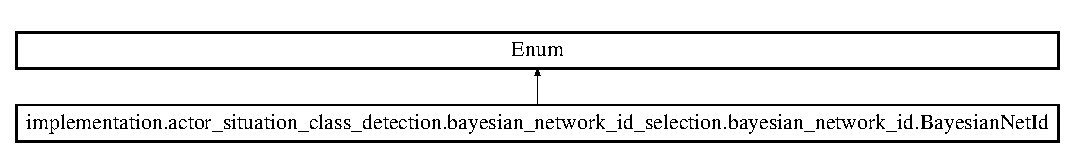
\includegraphics[height=1.671642cm]{classimplementation_1_1actor__situation__class__detection_1_1bayesian__network__id__selection_1_c01f1dacd43bed2d1110fc7cec61e664}
\end{center}
\end{figure}
\doxysubsection*{Static Public Attributes}
\begin{DoxyCompactItemize}
\item 
int \mbox{\hyperlink{classimplementation_1_1actor__situation__class__detection_1_1bayesian__network__id__selection_1_c01f1dacd43bed2d1110fc7cec61e664_a86a7fd55d6332f550538eae8fec3303a}{U\+N\+K\+N\+O\+WN}} = 1,
\item 
int \mbox{\hyperlink{classimplementation_1_1actor__situation__class__detection_1_1bayesian__network__id__selection_1_c01f1dacd43bed2d1110fc7cec61e664_a663104f7c0b4e8e9292e345994df3e8a}{T\+W\+O\+\_\+\+L\+A\+N\+E\+\_\+\+F\+O\+L\+L\+O\+W\+I\+N\+G\+\_\+\+E\+GO}} = 2,
\item 
int \mbox{\hyperlink{classimplementation_1_1actor__situation__class__detection_1_1bayesian__network__id__selection_1_c01f1dacd43bed2d1110fc7cec61e664_ae8a24c9833e1a84925277af449b4b2e2}{T\+W\+O\+\_\+\+L\+A\+N\+E\+\_\+\+F\+O\+L\+L\+O\+W\+I\+N\+G\+\_\+\+F\+R\+O\+N\+T\+\_\+\+V\+E\+H\+I\+C\+LE}} = 3,
\item 
int \mbox{\hyperlink{classimplementation_1_1actor__situation__class__detection_1_1bayesian__network__id__selection_1_c01f1dacd43bed2d1110fc7cec61e664_a80f21fbae9c3cfb9a17be8d96b9a2f2f}{T\+W\+O\+\_\+\+L\+A\+N\+E\+\_\+\+F\+O\+L\+L\+O\+W\+I\+N\+G\+\_\+\+S\+I\+D\+E\+\_\+\+V\+E\+H\+I\+C\+L\+E\+\_\+\+O\+N\+\_\+\+O\+T\+H\+E\+R\+\_\+\+L\+A\+N\+E\+\_\+\+L\+E\+FT}} = 4,
\item 
int \mbox{\hyperlink{classimplementation_1_1actor__situation__class__detection_1_1bayesian__network__id__selection_1_c01f1dacd43bed2d1110fc7cec61e664_ae4769da71090da6b10c9b68aa126efd2}{T\+W\+O\+\_\+\+L\+A\+N\+E\+\_\+\+F\+O\+L\+L\+O\+W\+I\+N\+G\+\_\+\+S\+I\+D\+E\+\_\+\+V\+E\+H\+I\+C\+L\+E\+\_\+\+O\+N\+\_\+\+O\+T\+H\+E\+R\+\_\+\+L\+A\+N\+E\+\_\+\+R\+I\+G\+HT}} = 5,
\item 
int \mbox{\hyperlink{classimplementation_1_1actor__situation__class__detection_1_1bayesian__network__id__selection_1_c01f1dacd43bed2d1110fc7cec61e664_a59f39091615e7ed03d13909bc9b663d3}{T\+W\+O\+\_\+\+L\+A\+N\+E\+\_\+\+F\+O\+L\+L\+O\+W\+I\+N\+G\+\_\+\+F\+R\+O\+N\+T\+\_\+\+V\+E\+H\+I\+C\+L\+E\+\_\+\+I\+N\+\_\+\+L\+A\+N\+E\+\_\+\+C\+H\+A\+N\+GE}} = 6
\end{DoxyCompactItemize}


\doxysubsection{Member Data Documentation}
\mbox{\Hypertarget{classimplementation_1_1actor__situation__class__detection_1_1bayesian__network__id__selection_1_c01f1dacd43bed2d1110fc7cec61e664_a663104f7c0b4e8e9292e345994df3e8a}\label{classimplementation_1_1actor__situation__class__detection_1_1bayesian__network__id__selection_1_c01f1dacd43bed2d1110fc7cec61e664_a663104f7c0b4e8e9292e345994df3e8a}} 
\index{implementation.actor\_situation\_class\_detection.bayesian\_network\_id\_selection.bayesian\_network\_id.BayesianNetId@{implementation.actor\_situation\_class\_detection.bayesian\_network\_id\_selection.bayesian\_network\_id.BayesianNetId}!TWO\_LANE\_FOLLOWING\_EGO@{TWO\_LANE\_FOLLOWING\_EGO}}
\index{TWO\_LANE\_FOLLOWING\_EGO@{TWO\_LANE\_FOLLOWING\_EGO}!implementation.actor\_situation\_class\_detection.bayesian\_network\_id\_selection.bayesian\_network\_id.BayesianNetId@{implementation.actor\_situation\_class\_detection.bayesian\_network\_id\_selection.bayesian\_network\_id.BayesianNetId}}
\doxysubsubsection{\texorpdfstring{TWO\_LANE\_FOLLOWING\_EGO}{TWO\_LANE\_FOLLOWING\_EGO}}
{\footnotesize\ttfamily int implementation.\+actor\+\_\+situation\+\_\+class\+\_\+detection.\+bayesian\+\_\+network\+\_\+id\+\_\+selection.\+bayesian\+\_\+network\+\_\+id.\+Bayesian\+Net\+Id.\+T\+W\+O\+\_\+\+L\+A\+N\+E\+\_\+\+F\+O\+L\+L\+O\+W\+I\+N\+G\+\_\+\+E\+GO = 2,\hspace{0.3cm}{\ttfamily [static]}}

\mbox{\Hypertarget{classimplementation_1_1actor__situation__class__detection_1_1bayesian__network__id__selection_1_c01f1dacd43bed2d1110fc7cec61e664_ae8a24c9833e1a84925277af449b4b2e2}\label{classimplementation_1_1actor__situation__class__detection_1_1bayesian__network__id__selection_1_c01f1dacd43bed2d1110fc7cec61e664_ae8a24c9833e1a84925277af449b4b2e2}} 
\index{implementation.actor\_situation\_class\_detection.bayesian\_network\_id\_selection.bayesian\_network\_id.BayesianNetId@{implementation.actor\_situation\_class\_detection.bayesian\_network\_id\_selection.bayesian\_network\_id.BayesianNetId}!TWO\_LANE\_FOLLOWING\_FRONT\_VEHICLE@{TWO\_LANE\_FOLLOWING\_FRONT\_VEHICLE}}
\index{TWO\_LANE\_FOLLOWING\_FRONT\_VEHICLE@{TWO\_LANE\_FOLLOWING\_FRONT\_VEHICLE}!implementation.actor\_situation\_class\_detection.bayesian\_network\_id\_selection.bayesian\_network\_id.BayesianNetId@{implementation.actor\_situation\_class\_detection.bayesian\_network\_id\_selection.bayesian\_network\_id.BayesianNetId}}
\doxysubsubsection{\texorpdfstring{TWO\_LANE\_FOLLOWING\_FRONT\_VEHICLE}{TWO\_LANE\_FOLLOWING\_FRONT\_VEHICLE}}
{\footnotesize\ttfamily int implementation.\+actor\+\_\+situation\+\_\+class\+\_\+detection.\+bayesian\+\_\+network\+\_\+id\+\_\+selection.\+bayesian\+\_\+network\+\_\+id.\+Bayesian\+Net\+Id.\+T\+W\+O\+\_\+\+L\+A\+N\+E\+\_\+\+F\+O\+L\+L\+O\+W\+I\+N\+G\+\_\+\+F\+R\+O\+N\+T\+\_\+\+V\+E\+H\+I\+C\+LE = 3,\hspace{0.3cm}{\ttfamily [static]}}

\mbox{\Hypertarget{classimplementation_1_1actor__situation__class__detection_1_1bayesian__network__id__selection_1_c01f1dacd43bed2d1110fc7cec61e664_a59f39091615e7ed03d13909bc9b663d3}\label{classimplementation_1_1actor__situation__class__detection_1_1bayesian__network__id__selection_1_c01f1dacd43bed2d1110fc7cec61e664_a59f39091615e7ed03d13909bc9b663d3}} 
\index{implementation.actor\_situation\_class\_detection.bayesian\_network\_id\_selection.bayesian\_network\_id.BayesianNetId@{implementation.actor\_situation\_class\_detection.bayesian\_network\_id\_selection.bayesian\_network\_id.BayesianNetId}!TWO\_LANE\_FOLLOWING\_FRONT\_VEHICLE\_IN\_LANE\_CHANGE@{TWO\_LANE\_FOLLOWING\_FRONT\_VEHICLE\_IN\_LANE\_CHANGE}}
\index{TWO\_LANE\_FOLLOWING\_FRONT\_VEHICLE\_IN\_LANE\_CHANGE@{TWO\_LANE\_FOLLOWING\_FRONT\_VEHICLE\_IN\_LANE\_CHANGE}!implementation.actor\_situation\_class\_detection.bayesian\_network\_id\_selection.bayesian\_network\_id.BayesianNetId@{implementation.actor\_situation\_class\_detection.bayesian\_network\_id\_selection.bayesian\_network\_id.BayesianNetId}}
\doxysubsubsection{\texorpdfstring{TWO\_LANE\_FOLLOWING\_FRONT\_VEHICLE\_IN\_LANE\_CHANGE}{TWO\_LANE\_FOLLOWING\_FRONT\_VEHICLE\_IN\_LANE\_CHANGE}}
{\footnotesize\ttfamily int implementation.\+actor\+\_\+situation\+\_\+class\+\_\+detection.\+bayesian\+\_\+network\+\_\+id\+\_\+selection.\+bayesian\+\_\+network\+\_\+id.\+Bayesian\+Net\+Id.\+T\+W\+O\+\_\+\+L\+A\+N\+E\+\_\+\+F\+O\+L\+L\+O\+W\+I\+N\+G\+\_\+\+F\+R\+O\+N\+T\+\_\+\+V\+E\+H\+I\+C\+L\+E\+\_\+\+I\+N\+\_\+\+L\+A\+N\+E\+\_\+\+C\+H\+A\+N\+GE = 6\hspace{0.3cm}{\ttfamily [static]}}

\mbox{\Hypertarget{classimplementation_1_1actor__situation__class__detection_1_1bayesian__network__id__selection_1_c01f1dacd43bed2d1110fc7cec61e664_a80f21fbae9c3cfb9a17be8d96b9a2f2f}\label{classimplementation_1_1actor__situation__class__detection_1_1bayesian__network__id__selection_1_c01f1dacd43bed2d1110fc7cec61e664_a80f21fbae9c3cfb9a17be8d96b9a2f2f}} 
\index{implementation.actor\_situation\_class\_detection.bayesian\_network\_id\_selection.bayesian\_network\_id.BayesianNetId@{implementation.actor\_situation\_class\_detection.bayesian\_network\_id\_selection.bayesian\_network\_id.BayesianNetId}!TWO\_LANE\_FOLLOWING\_SIDE\_VEHICLE\_ON\_OTHER\_LANE\_LEFT@{TWO\_LANE\_FOLLOWING\_SIDE\_VEHICLE\_ON\_OTHER\_LANE\_LEFT}}
\index{TWO\_LANE\_FOLLOWING\_SIDE\_VEHICLE\_ON\_OTHER\_LANE\_LEFT@{TWO\_LANE\_FOLLOWING\_SIDE\_VEHICLE\_ON\_OTHER\_LANE\_LEFT}!implementation.actor\_situation\_class\_detection.bayesian\_network\_id\_selection.bayesian\_network\_id.BayesianNetId@{implementation.actor\_situation\_class\_detection.bayesian\_network\_id\_selection.bayesian\_network\_id.BayesianNetId}}
\doxysubsubsection{\texorpdfstring{TWO\_LANE\_FOLLOWING\_SIDE\_VEHICLE\_ON\_OTHER\_LANE\_LEFT}{TWO\_LANE\_FOLLOWING\_SIDE\_VEHICLE\_ON\_OTHER\_LANE\_LEFT}}
{\footnotesize\ttfamily int implementation.\+actor\+\_\+situation\+\_\+class\+\_\+detection.\+bayesian\+\_\+network\+\_\+id\+\_\+selection.\+bayesian\+\_\+network\+\_\+id.\+Bayesian\+Net\+Id.\+T\+W\+O\+\_\+\+L\+A\+N\+E\+\_\+\+F\+O\+L\+L\+O\+W\+I\+N\+G\+\_\+\+S\+I\+D\+E\+\_\+\+V\+E\+H\+I\+C\+L\+E\+\_\+\+O\+N\+\_\+\+O\+T\+H\+E\+R\+\_\+\+L\+A\+N\+E\+\_\+\+L\+E\+FT = 4,\hspace{0.3cm}{\ttfamily [static]}}

\mbox{\Hypertarget{classimplementation_1_1actor__situation__class__detection_1_1bayesian__network__id__selection_1_c01f1dacd43bed2d1110fc7cec61e664_ae4769da71090da6b10c9b68aa126efd2}\label{classimplementation_1_1actor__situation__class__detection_1_1bayesian__network__id__selection_1_c01f1dacd43bed2d1110fc7cec61e664_ae4769da71090da6b10c9b68aa126efd2}} 
\index{implementation.actor\_situation\_class\_detection.bayesian\_network\_id\_selection.bayesian\_network\_id.BayesianNetId@{implementation.actor\_situation\_class\_detection.bayesian\_network\_id\_selection.bayesian\_network\_id.BayesianNetId}!TWO\_LANE\_FOLLOWING\_SIDE\_VEHICLE\_ON\_OTHER\_LANE\_RIGHT@{TWO\_LANE\_FOLLOWING\_SIDE\_VEHICLE\_ON\_OTHER\_LANE\_RIGHT}}
\index{TWO\_LANE\_FOLLOWING\_SIDE\_VEHICLE\_ON\_OTHER\_LANE\_RIGHT@{TWO\_LANE\_FOLLOWING\_SIDE\_VEHICLE\_ON\_OTHER\_LANE\_RIGHT}!implementation.actor\_situation\_class\_detection.bayesian\_network\_id\_selection.bayesian\_network\_id.BayesianNetId@{implementation.actor\_situation\_class\_detection.bayesian\_network\_id\_selection.bayesian\_network\_id.BayesianNetId}}
\doxysubsubsection{\texorpdfstring{TWO\_LANE\_FOLLOWING\_SIDE\_VEHICLE\_ON\_OTHER\_LANE\_RIGHT}{TWO\_LANE\_FOLLOWING\_SIDE\_VEHICLE\_ON\_OTHER\_LANE\_RIGHT}}
{\footnotesize\ttfamily int implementation.\+actor\+\_\+situation\+\_\+class\+\_\+detection.\+bayesian\+\_\+network\+\_\+id\+\_\+selection.\+bayesian\+\_\+network\+\_\+id.\+Bayesian\+Net\+Id.\+T\+W\+O\+\_\+\+L\+A\+N\+E\+\_\+\+F\+O\+L\+L\+O\+W\+I\+N\+G\+\_\+\+S\+I\+D\+E\+\_\+\+V\+E\+H\+I\+C\+L\+E\+\_\+\+O\+N\+\_\+\+O\+T\+H\+E\+R\+\_\+\+L\+A\+N\+E\+\_\+\+R\+I\+G\+HT = 5,\hspace{0.3cm}{\ttfamily [static]}}

\mbox{\Hypertarget{classimplementation_1_1actor__situation__class__detection_1_1bayesian__network__id__selection_1_c01f1dacd43bed2d1110fc7cec61e664_a86a7fd55d6332f550538eae8fec3303a}\label{classimplementation_1_1actor__situation__class__detection_1_1bayesian__network__id__selection_1_c01f1dacd43bed2d1110fc7cec61e664_a86a7fd55d6332f550538eae8fec3303a}} 
\index{implementation.actor\_situation\_class\_detection.bayesian\_network\_id\_selection.bayesian\_network\_id.BayesianNetId@{implementation.actor\_situation\_class\_detection.bayesian\_network\_id\_selection.bayesian\_network\_id.BayesianNetId}!UNKNOWN@{UNKNOWN}}
\index{UNKNOWN@{UNKNOWN}!implementation.actor\_situation\_class\_detection.bayesian\_network\_id\_selection.bayesian\_network\_id.BayesianNetId@{implementation.actor\_situation\_class\_detection.bayesian\_network\_id\_selection.bayesian\_network\_id.BayesianNetId}}
\doxysubsubsection{\texorpdfstring{UNKNOWN}{UNKNOWN}}
{\footnotesize\ttfamily int implementation.\+actor\+\_\+situation\+\_\+class\+\_\+detection.\+bayesian\+\_\+network\+\_\+id\+\_\+selection.\+bayesian\+\_\+network\+\_\+id.\+Bayesian\+Net\+Id.\+U\+N\+K\+N\+O\+WN = 1,\hspace{0.3cm}{\ttfamily [static]}}



The documentation for this class was generated from the following file\+:\begin{DoxyCompactItemize}
\item 
implementation/actor\+\_\+situation\+\_\+class\+\_\+detection/bayesian\+\_\+network\+\_\+id\+\_\+selection/\mbox{\hyperlink{bayesian__network__id_8py}{bayesian\+\_\+network\+\_\+id.\+py}}\end{DoxyCompactItemize}

\hypertarget{classimplementation_1_1bayesian__network_1_1model__generation_1_1config__template_1_1_bayesian_network_config}{}\doxysection{implementation.\+bayesian\+\_\+network.\+model\+\_\+generation.\+config\+\_\+template.\+Bayesian\+Network\+Config Class Reference}
\label{classimplementation_1_1bayesian__network_1_1model__generation_1_1config__template_1_1_bayesian_network_config}\index{implementation.bayesian\_network.model\_generation.config\_template.BayesianNetworkConfig@{implementation.bayesian\_network.model\_generation.config\_template.BayesianNetworkConfig}}


B\+E\+G\+IN L\+I\+C\+E\+N\+SE B\+L\+O\+CK \#\#\#\#\#\#\#\#\#\#\#\#\#\#\#\#\#\#\#\#\#\#\#\#\#\#\#\#\#\#\#.  


\doxysubsection*{Public Member Functions}
\begin{DoxyCompactItemize}
\item 
None \mbox{\hyperlink{classimplementation_1_1bayesian__network_1_1model__generation_1_1config__template_1_1_bayesian_network_config_a5279537a100aeb5558c76354de5c76c9}{\+\_\+\+\_\+init\+\_\+\+\_\+}} (self)
\item 
None \mbox{\hyperlink{classimplementation_1_1bayesian__network_1_1model__generation_1_1config__template_1_1_bayesian_network_config_a913ec95ad29ab4da524010da4b7d7d03}{update\+\_\+dra\+\_\+data}} (self, \char`\"{}S\+I\+N\+A\+D\+R\+A\+Risk\+Sensor\+Data\char`\"{} dra\+\_\+data)
\end{DoxyCompactItemize}
\doxysubsection*{Public Attributes}
\begin{DoxyCompactItemize}
\item 
\mbox{\hyperlink{classimplementation_1_1bayesian__network_1_1model__generation_1_1config__template_1_1_bayesian_network_config_ae3c593ce1d24a9472bab06a72ff0c70f}{dra\+\_\+data}}
\end{DoxyCompactItemize}


\doxysubsection{Detailed Description}
B\+E\+G\+IN L\+I\+C\+E\+N\+SE B\+L\+O\+CK \#\#\#\#\#\#\#\#\#\#\#\#\#\#\#\#\#\#\#\#\#\#\#\#\#\#\#\#\#\#\#. 

Copyright (C) 2021 Fraunhofer I\+E\+SE

S\+P\+D\+X-\/\+License-\/\+Identifier\+: L\+G\+P\+L-\/2.\+1-\/only

E\+ND L\+I\+C\+E\+N\+SE B\+L\+O\+CK \#\#\#\#\#\#\#\#\#\#\#\#\#\#\#\#\#\#\#\#\#\#\#\#\#\#\#\#\#\#\#\#\#

\begin{DoxyVerb}Bayesian network config to change the node's outcomes dependent
on the received DRA data.
\end{DoxyVerb}
 

\doxysubsection{Constructor \& Destructor Documentation}
\mbox{\Hypertarget{classimplementation_1_1bayesian__network_1_1model__generation_1_1config__template_1_1_bayesian_network_config_a5279537a100aeb5558c76354de5c76c9}\label{classimplementation_1_1bayesian__network_1_1model__generation_1_1config__template_1_1_bayesian_network_config_a5279537a100aeb5558c76354de5c76c9}} 
\index{implementation.bayesian\_network.model\_generation.config\_template.BayesianNetworkConfig@{implementation.bayesian\_network.model\_generation.config\_template.BayesianNetworkConfig}!\_\_init\_\_@{\_\_init\_\_}}
\index{\_\_init\_\_@{\_\_init\_\_}!implementation.bayesian\_network.model\_generation.config\_template.BayesianNetworkConfig@{implementation.bayesian\_network.model\_generation.config\_template.BayesianNetworkConfig}}
\doxysubsubsection{\texorpdfstring{\_\_init\_\_()}{\_\_init\_\_()}}
{\footnotesize\ttfamily  None implementation.\+bayesian\+\_\+network.\+model\+\_\+generation.\+config\+\_\+template.\+Bayesian\+Network\+Config.\+\_\+\+\_\+init\+\_\+\+\_\+ (\begin{DoxyParamCaption}\item[{}]{self }\end{DoxyParamCaption})}

\begin{DoxyVerb}Initialize the (simulator's) DRA data.\end{DoxyVerb}
 

\doxysubsection{Member Function Documentation}
\mbox{\Hypertarget{classimplementation_1_1bayesian__network_1_1model__generation_1_1config__template_1_1_bayesian_network_config_a913ec95ad29ab4da524010da4b7d7d03}\label{classimplementation_1_1bayesian__network_1_1model__generation_1_1config__template_1_1_bayesian_network_config_a913ec95ad29ab4da524010da4b7d7d03}} 
\index{implementation.bayesian\_network.model\_generation.config\_template.BayesianNetworkConfig@{implementation.bayesian\_network.model\_generation.config\_template.BayesianNetworkConfig}!update\_dra\_data@{update\_dra\_data}}
\index{update\_dra\_data@{update\_dra\_data}!implementation.bayesian\_network.model\_generation.config\_template.BayesianNetworkConfig@{implementation.bayesian\_network.model\_generation.config\_template.BayesianNetworkConfig}}
\doxysubsubsection{\texorpdfstring{update\_dra\_data()}{update\_dra\_data()}}
{\footnotesize\ttfamily  None implementation.\+bayesian\+\_\+network.\+model\+\_\+generation.\+config\+\_\+template.\+Bayesian\+Network\+Config.\+update\+\_\+dra\+\_\+data (\begin{DoxyParamCaption}\item[{}]{self,  }\item[{\char`\"{}S\+I\+N\+A\+D\+R\+A\+Risk\+Sensor\+Data\char`\"{}}]{dra\+\_\+data }\end{DoxyParamCaption})}

\begin{DoxyVerb}Updates the saved DRA input feature data class instance.

Parameters
----------
dra_data : SINADRARiskSensorData
    Latest DRA input feature data class instance for the Bayesian network.
\end{DoxyVerb}
 

\doxysubsection{Member Data Documentation}
\mbox{\Hypertarget{classimplementation_1_1bayesian__network_1_1model__generation_1_1config__template_1_1_bayesian_network_config_ae3c593ce1d24a9472bab06a72ff0c70f}\label{classimplementation_1_1bayesian__network_1_1model__generation_1_1config__template_1_1_bayesian_network_config_ae3c593ce1d24a9472bab06a72ff0c70f}} 
\index{implementation.bayesian\_network.model\_generation.config\_template.BayesianNetworkConfig@{implementation.bayesian\_network.model\_generation.config\_template.BayesianNetworkConfig}!dra\_data@{dra\_data}}
\index{dra\_data@{dra\_data}!implementation.bayesian\_network.model\_generation.config\_template.BayesianNetworkConfig@{implementation.bayesian\_network.model\_generation.config\_template.BayesianNetworkConfig}}
\doxysubsubsection{\texorpdfstring{dra\_data}{dra\_data}}
{\footnotesize\ttfamily implementation.\+bayesian\+\_\+network.\+model\+\_\+generation.\+config\+\_\+template.\+Bayesian\+Network\+Config.\+dra\+\_\+data}



The documentation for this class was generated from the following file\+:\begin{DoxyCompactItemize}
\item 
implementation/bayesian\+\_\+network/model\+\_\+generation/\mbox{\hyperlink{config__template_8py}{config\+\_\+template.\+py}}\end{DoxyCompactItemize}

\hypertarget{classbayesian__network__config_1_1_bayesian_network_config}{}\doxysection{bayesian\+\_\+network\+\_\+config.\+Bayesian\+Network\+Config Class Reference}
\label{classbayesian__network__config_1_1_bayesian_network_config}\index{bayesian\_network\_config.BayesianNetworkConfig@{bayesian\_network\_config.BayesianNetworkConfig}}


B\+E\+G\+IN L\+I\+C\+E\+N\+SE B\+L\+O\+CK \#\#\#\#\#\#\#\#\#\#\#\#\#\#\#\#\#\#\#\#\#\#\#\#\#\#\#\#\#\#\#.  


\doxysubsection*{Public Member Functions}
\begin{DoxyCompactItemize}
\item 
None \mbox{\hyperlink{classbayesian__network__config_1_1_bayesian_network_config_aba849261705cd87984939e8a61a7e8e7}{\+\_\+\+\_\+init\+\_\+\+\_\+}} (self)
\item 
None \mbox{\hyperlink{classbayesian__network__config_1_1_bayesian_network_config_abd9217382590924437bb866e25f47b1a}{update\+\_\+dra\+\_\+data}} (self, \char`\"{}S\+I\+N\+A\+D\+R\+A\+Risk\+Sensor\+Data\char`\"{} dra\+\_\+data)
\item 
def \mbox{\hyperlink{classbayesian__network__config_1_1_bayesian_network_config_a49f488a98830cd4781609a426aab8f7c}{node\+\_\+\+T\+TC}} (self)
\item 
def \mbox{\hyperlink{classbayesian__network__config_1_1_bayesian_network_config_a813f87173ae162e2463b86d2fbf7f287}{node\+\_\+\+T\+T\+C\+\_\+\+Measurement\+\_\+\+Uncertainty}} (self)
\item 
def \mbox{\hyperlink{classbayesian__network__config_1_1_bayesian_network_config_a0aff21732724921c5b734e4cc2128711}{node\+\_\+\+Measured\+\_\+\+T\+TC}} (self)
\item 
def \mbox{\hyperlink{classbayesian__network__config_1_1_bayesian_network_config_a7e92e0763a594ce2d1ac0e6cf4ed6658}{node\+\_\+\+Heavy\+Rain}} (self)
\item 
def \mbox{\hyperlink{classbayesian__network__config_1_1_bayesian_network_config_a14bac441795a8f3c96df9342dff6ecc2}{node\+\_\+\+F\+V\+View\+Range}} (self)
\item 
def \mbox{\hyperlink{classbayesian__network__config_1_1_bayesian_network_config_aa4e512eed678233616fbc648e8a5d973}{node\+\_\+\+F\+V\+\_\+\+Situation\+\_\+\+Perception}} (self)
\item 
def \mbox{\hyperlink{classbayesian__network__config_1_1_bayesian_network_config_a73e6055c566983256fceb8f6c587d20a}{node\+\_\+\+F\+V\+\_\+\+Situation\+\_\+\+Assessment}} (self)
\item 
def \mbox{\hyperlink{classbayesian__network__config_1_1_bayesian_network_config_aa63fd1483c8ff02d6bc7c9482a59cad5}{node\+\_\+\+F\+V\+\_\+\+Maneuver\+\_\+\+Decision}} (self)
\item 
def \mbox{\hyperlink{classbayesian__network__config_1_1_bayesian_network_config_afe1f290bda7493ebf0098c0c69ec267b}{node\+\_\+\+F\+V\+\_\+\+Front\+\_\+\+Existence}} (self)
\item 
def \mbox{\hyperlink{classbayesian__network__config_1_1_bayesian_network_config_a424061edb518c981c0e1ceed918a6d2f}{node\+\_\+\+F\+V\+\_\+\+Braking\+\_\+\+Behavior}} (self)
\item 
def \mbox{\hyperlink{classbayesian__network__config_1_1_bayesian_network_config_a7f212c99308978eef668419727075a07}{node\+\_\+\+F\+V\+Type}} (self)
\item 
def \mbox{\hyperlink{classbayesian__network__config_1_1_bayesian_network_config_aff3733f4b57dcb4c4cbc0184ea07c133}{node\+\_\+\+Ego\+\_\+\+F\+V\+\_\+\+Perception}} (self)
\item 
def \mbox{\hyperlink{classbayesian__network__config_1_1_bayesian_network_config_a2f2e6cb9c1179565953917ff4f56935c}{node\+\_\+\+Predicted\+\_\+\+F\+V\+\_\+\+Braking\+\_\+\+Behavior}} (self)
\item 
None \mbox{\hyperlink{classbayesian__network__config_1_1_bayesian_network_config_aba849261705cd87984939e8a61a7e8e7}{\+\_\+\+\_\+init\+\_\+\+\_\+}} (self)
\item 
None \mbox{\hyperlink{classbayesian__network__config_1_1_bayesian_network_config_abd9217382590924437bb866e25f47b1a}{update\+\_\+dra\+\_\+data}} (self, \char`\"{}S\+I\+N\+A\+D\+R\+A\+Risk\+Sensor\+Data\char`\"{} dra\+\_\+data)
\item 
def \mbox{\hyperlink{classbayesian__network__config_1_1_bayesian_network_config_a9a6e2aefc96155fcdd4a825b1defbe76}{node\+\_\+\+Lane\+\_\+\+Ends}} (self)
\item 
def \mbox{\hyperlink{classbayesian__network__config_1_1_bayesian_network_config_a597ae7d023043c246dc2e31ceb125eec}{node\+\_\+\+Lane\+\_\+\+Change\+\_\+\+Intent}} (self)
\item 
def \mbox{\hyperlink{classbayesian__network__config_1_1_bayesian_network_config_a86c973a53f1f78567b32ffa68cea467a}{node\+\_\+\+Gap\+\_\+\+Availability}} (self)
\item 
def \mbox{\hyperlink{classbayesian__network__config_1_1_bayesian_network_config_a86c960e95351259be8f751f98ac91aa5}{node\+\_\+\+Gap\+\_\+\+Acceptance}} (self)
\item 
def \mbox{\hyperlink{classbayesian__network__config_1_1_bayesian_network_config_a7e92e0763a594ce2d1ac0e6cf4ed6658}{node\+\_\+\+Heavy\+Rain}} (self)
\item 
def \mbox{\hyperlink{classbayesian__network__config_1_1_bayesian_network_config_a14bac441795a8f3c96df9342dff6ecc2}{node\+\_\+\+F\+V\+View\+Range}} (self)
\item 
def \mbox{\hyperlink{classbayesian__network__config_1_1_bayesian_network_config_a1eb21f6bfb872d4c8773615d265c3727}{node\+\_\+\+S\+V\+\_\+\+Situation\+\_\+\+Perception}} (self)
\item 
def \mbox{\hyperlink{classbayesian__network__config_1_1_bayesian_network_config_a542c4ed5d49ca145684cfcff7a6e90f6}{node\+\_\+\+S\+V\+\_\+\+Situation\+\_\+\+Assessment}} (self)
\item 
def \mbox{\hyperlink{classbayesian__network__config_1_1_bayesian_network_config_a978dd92b9826d22d6e521630d0a34379}{node\+\_\+\+S\+V\+\_\+\+Maneuver\+\_\+\+Decision}} (self)
\item 
def \mbox{\hyperlink{classbayesian__network__config_1_1_bayesian_network_config_a6510c23dac8fb0c36ee38283e5815d54}{node\+\_\+\+S\+V\+\_\+\+Cutin\+\_\+\+Behavior}} (self)
\item 
def \mbox{\hyperlink{classbayesian__network__config_1_1_bayesian_network_config_aff3733f4b57dcb4c4cbc0184ea07c133}{node\+\_\+\+Ego\+\_\+\+F\+V\+\_\+\+Perception}} (self)
\item 
def \mbox{\hyperlink{classbayesian__network__config_1_1_bayesian_network_config_a94ce3d69a47a081032bbc9b6461645e9}{node\+\_\+\+Predicted\+\_\+\+S\+V\+\_\+\+Cut\+\_\+\+In\+\_\+\+Behavior}} (self)
\item 
def \mbox{\hyperlink{classbayesian__network__config_1_1_bayesian_network_config_a27d247927ce168025568fdf0d467b78d}{node\+\_\+\+Steering\+\_\+\+Angle}} (self)
\item 
def \mbox{\hyperlink{classbayesian__network__config_1_1_bayesian_network_config_ac9fee7655297b9617622e9c4d4669a23}{node\+\_\+\+Turn\+\_\+\+Indicator}} (self)
\item 
def \mbox{\hyperlink{classbayesian__network__config_1_1_bayesian_network_config_a3cf26cc8ccfdff070ff06302ce79f4f5}{node\+\_\+\+Distance\+\_\+\+Center}} (self)
\end{DoxyCompactItemize}
\doxysubsection*{Public Attributes}
\begin{DoxyCompactItemize}
\item 
\mbox{\hyperlink{classbayesian__network__config_1_1_bayesian_network_config_aa80a7563c87c07c57e7c1318e147353e}{dra\+\_\+data}}
\end{DoxyCompactItemize}


\doxysubsection{Detailed Description}
B\+E\+G\+IN L\+I\+C\+E\+N\+SE B\+L\+O\+CK \#\#\#\#\#\#\#\#\#\#\#\#\#\#\#\#\#\#\#\#\#\#\#\#\#\#\#\#\#\#\#. 

Copyright (C) 2021 Fraunhofer I\+E\+SE

S\+P\+D\+X-\/\+License-\/\+Identifier\+: L\+G\+P\+L-\/2.\+1-\/only

E\+ND L\+I\+C\+E\+N\+SE B\+L\+O\+CK \#\#\#\#\#\#\#\#\#\#\#\#\#\#\#\#\#\#\#\#\#\#\#\#\#\#\#\#\#\#\#\#\#

\begin{DoxyVerb}Bayesian network config to change the node's outcomes dependent
on the received DRA data.
\end{DoxyVerb}
 

\doxysubsection{Constructor \& Destructor Documentation}
\mbox{\Hypertarget{classbayesian__network__config_1_1_bayesian_network_config_aba849261705cd87984939e8a61a7e8e7}\label{classbayesian__network__config_1_1_bayesian_network_config_aba849261705cd87984939e8a61a7e8e7}} 
\index{bayesian\_network\_config.BayesianNetworkConfig@{bayesian\_network\_config.BayesianNetworkConfig}!\_\_init\_\_@{\_\_init\_\_}}
\index{\_\_init\_\_@{\_\_init\_\_}!bayesian\_network\_config.BayesianNetworkConfig@{bayesian\_network\_config.BayesianNetworkConfig}}
\doxysubsubsection{\texorpdfstring{\_\_init\_\_()}{\_\_init\_\_()}\hspace{0.1cm}{\footnotesize\ttfamily [1/2]}}
{\footnotesize\ttfamily  None bayesian\+\_\+network\+\_\+config.\+Bayesian\+Network\+Config.\+\_\+\+\_\+init\+\_\+\+\_\+ (\begin{DoxyParamCaption}\item[{}]{self }\end{DoxyParamCaption})}

\begin{DoxyVerb}Initialize the (simulator's) DRA data.\end{DoxyVerb}
 \mbox{\Hypertarget{classbayesian__network__config_1_1_bayesian_network_config_aba849261705cd87984939e8a61a7e8e7}\label{classbayesian__network__config_1_1_bayesian_network_config_aba849261705cd87984939e8a61a7e8e7}} 
\index{bayesian\_network\_config.BayesianNetworkConfig@{bayesian\_network\_config.BayesianNetworkConfig}!\_\_init\_\_@{\_\_init\_\_}}
\index{\_\_init\_\_@{\_\_init\_\_}!bayesian\_network\_config.BayesianNetworkConfig@{bayesian\_network\_config.BayesianNetworkConfig}}
\doxysubsubsection{\texorpdfstring{\_\_init\_\_()}{\_\_init\_\_()}\hspace{0.1cm}{\footnotesize\ttfamily [2/2]}}
{\footnotesize\ttfamily  None bayesian\+\_\+network\+\_\+config.\+Bayesian\+Network\+Config.\+\_\+\+\_\+init\+\_\+\+\_\+ (\begin{DoxyParamCaption}\item[{}]{self }\end{DoxyParamCaption})}

\begin{DoxyVerb}Initialize the (simulator's) DRA data.\end{DoxyVerb}
 

\doxysubsection{Member Function Documentation}
\mbox{\Hypertarget{classbayesian__network__config_1_1_bayesian_network_config_a3cf26cc8ccfdff070ff06302ce79f4f5}\label{classbayesian__network__config_1_1_bayesian_network_config_a3cf26cc8ccfdff070ff06302ce79f4f5}} 
\index{bayesian\_network\_config.BayesianNetworkConfig@{bayesian\_network\_config.BayesianNetworkConfig}!node\_Distance\_Center@{node\_Distance\_Center}}
\index{node\_Distance\_Center@{node\_Distance\_Center}!bayesian\_network\_config.BayesianNetworkConfig@{bayesian\_network\_config.BayesianNetworkConfig}}
\doxysubsubsection{\texorpdfstring{node\_Distance\_Center()}{node\_Distance\_Center()}}
{\footnotesize\ttfamily def bayesian\+\_\+network\+\_\+config.\+Bayesian\+Network\+Config.\+node\+\_\+\+Distance\+\_\+\+Center (\begin{DoxyParamCaption}\item[{}]{self }\end{DoxyParamCaption})}

\begin{DoxyVerb}Method for the CPT node 'Distance_Center' that allows setting the node as output node, 
and allows changing this nodes outcomes for the Bayesian network inference.

Returns
-------
Tuple[bool, Dict[str, float]]
    Flag whether this node is an output node, and dictionary with the node outcome IDs as keys 
    and the corresponding probabilities as values.
\end{DoxyVerb}
 \mbox{\Hypertarget{classbayesian__network__config_1_1_bayesian_network_config_aff3733f4b57dcb4c4cbc0184ea07c133}\label{classbayesian__network__config_1_1_bayesian_network_config_aff3733f4b57dcb4c4cbc0184ea07c133}} 
\index{bayesian\_network\_config.BayesianNetworkConfig@{bayesian\_network\_config.BayesianNetworkConfig}!node\_Ego\_FV\_Perception@{node\_Ego\_FV\_Perception}}
\index{node\_Ego\_FV\_Perception@{node\_Ego\_FV\_Perception}!bayesian\_network\_config.BayesianNetworkConfig@{bayesian\_network\_config.BayesianNetworkConfig}}
\doxysubsubsection{\texorpdfstring{node\_Ego\_FV\_Perception()}{node\_Ego\_FV\_Perception()}\hspace{0.1cm}{\footnotesize\ttfamily [1/2]}}
{\footnotesize\ttfamily def bayesian\+\_\+network\+\_\+config.\+Bayesian\+Network\+Config.\+node\+\_\+\+Ego\+\_\+\+F\+V\+\_\+\+Perception (\begin{DoxyParamCaption}\item[{}]{self }\end{DoxyParamCaption})}

\begin{DoxyVerb}Method for the CPT node 'Ego_FV_Perception' that allows setting the node as output node,
and allows changing this nodes outcomes for the Bayesian network inference.

Returns
-------
Tuple[bool, Dict[str, float]]
    Flag whether this node is an output node, and dictionary with the node outcome IDs as keys
    and the corresponding probabilities as values.
\end{DoxyVerb}
 \mbox{\Hypertarget{classbayesian__network__config_1_1_bayesian_network_config_aff3733f4b57dcb4c4cbc0184ea07c133}\label{classbayesian__network__config_1_1_bayesian_network_config_aff3733f4b57dcb4c4cbc0184ea07c133}} 
\index{bayesian\_network\_config.BayesianNetworkConfig@{bayesian\_network\_config.BayesianNetworkConfig}!node\_Ego\_FV\_Perception@{node\_Ego\_FV\_Perception}}
\index{node\_Ego\_FV\_Perception@{node\_Ego\_FV\_Perception}!bayesian\_network\_config.BayesianNetworkConfig@{bayesian\_network\_config.BayesianNetworkConfig}}
\doxysubsubsection{\texorpdfstring{node\_Ego\_FV\_Perception()}{node\_Ego\_FV\_Perception()}\hspace{0.1cm}{\footnotesize\ttfamily [2/2]}}
{\footnotesize\ttfamily def bayesian\+\_\+network\+\_\+config.\+Bayesian\+Network\+Config.\+node\+\_\+\+Ego\+\_\+\+F\+V\+\_\+\+Perception (\begin{DoxyParamCaption}\item[{}]{self }\end{DoxyParamCaption})}

\begin{DoxyVerb}Method for the CPT node 'Ego_FV_Perception' that allows setting the node as output node, 
and allows changing this nodes outcomes for the Bayesian network inference.

Returns
-------
Tuple[bool, Dict[str, float]]
    Flag whether this node is an output node, and dictionary with the node outcome IDs as keys 
    and the corresponding probabilities as values.
\end{DoxyVerb}
 \mbox{\Hypertarget{classbayesian__network__config_1_1_bayesian_network_config_a424061edb518c981c0e1ceed918a6d2f}\label{classbayesian__network__config_1_1_bayesian_network_config_a424061edb518c981c0e1ceed918a6d2f}} 
\index{bayesian\_network\_config.BayesianNetworkConfig@{bayesian\_network\_config.BayesianNetworkConfig}!node\_FV\_Braking\_Behavior@{node\_FV\_Braking\_Behavior}}
\index{node\_FV\_Braking\_Behavior@{node\_FV\_Braking\_Behavior}!bayesian\_network\_config.BayesianNetworkConfig@{bayesian\_network\_config.BayesianNetworkConfig}}
\doxysubsubsection{\texorpdfstring{node\_FV\_Braking\_Behavior()}{node\_FV\_Braking\_Behavior()}}
{\footnotesize\ttfamily def bayesian\+\_\+network\+\_\+config.\+Bayesian\+Network\+Config.\+node\+\_\+\+F\+V\+\_\+\+Braking\+\_\+\+Behavior (\begin{DoxyParamCaption}\item[{}]{self }\end{DoxyParamCaption})}

\begin{DoxyVerb}Method for the CPT node 'FV_Braking_Behavior' that allows setting the node as output node,
and allows changing this nodes outcomes for the Bayesian network inference.

Returns
-------
Tuple[bool, Dict[str, float]]
    Flag whether this node is an output node, and dictionary with the node outcome IDs as keys
    and the corresponding probabilities as values.
\end{DoxyVerb}
 \mbox{\Hypertarget{classbayesian__network__config_1_1_bayesian_network_config_afe1f290bda7493ebf0098c0c69ec267b}\label{classbayesian__network__config_1_1_bayesian_network_config_afe1f290bda7493ebf0098c0c69ec267b}} 
\index{bayesian\_network\_config.BayesianNetworkConfig@{bayesian\_network\_config.BayesianNetworkConfig}!node\_FV\_Front\_Existence@{node\_FV\_Front\_Existence}}
\index{node\_FV\_Front\_Existence@{node\_FV\_Front\_Existence}!bayesian\_network\_config.BayesianNetworkConfig@{bayesian\_network\_config.BayesianNetworkConfig}}
\doxysubsubsection{\texorpdfstring{node\_FV\_Front\_Existence()}{node\_FV\_Front\_Existence()}}
{\footnotesize\ttfamily def bayesian\+\_\+network\+\_\+config.\+Bayesian\+Network\+Config.\+node\+\_\+\+F\+V\+\_\+\+Front\+\_\+\+Existence (\begin{DoxyParamCaption}\item[{}]{self }\end{DoxyParamCaption})}

\begin{DoxyVerb}Method for the CPT node 'FV_Front_Existence' that allows setting the node as output node,
and allows changing this nodes outcomes for the Bayesian network inference.

Returns
-------
Tuple[bool, Dict[str, float]]
    Flag whether this node is an output node, and dictionary with the node outcome IDs as keys
    and the corresponding probabilities as values.
\end{DoxyVerb}
 \mbox{\Hypertarget{classbayesian__network__config_1_1_bayesian_network_config_aa63fd1483c8ff02d6bc7c9482a59cad5}\label{classbayesian__network__config_1_1_bayesian_network_config_aa63fd1483c8ff02d6bc7c9482a59cad5}} 
\index{bayesian\_network\_config.BayesianNetworkConfig@{bayesian\_network\_config.BayesianNetworkConfig}!node\_FV\_Maneuver\_Decision@{node\_FV\_Maneuver\_Decision}}
\index{node\_FV\_Maneuver\_Decision@{node\_FV\_Maneuver\_Decision}!bayesian\_network\_config.BayesianNetworkConfig@{bayesian\_network\_config.BayesianNetworkConfig}}
\doxysubsubsection{\texorpdfstring{node\_FV\_Maneuver\_Decision()}{node\_FV\_Maneuver\_Decision()}}
{\footnotesize\ttfamily def bayesian\+\_\+network\+\_\+config.\+Bayesian\+Network\+Config.\+node\+\_\+\+F\+V\+\_\+\+Maneuver\+\_\+\+Decision (\begin{DoxyParamCaption}\item[{}]{self }\end{DoxyParamCaption})}

\begin{DoxyVerb}Method for the CPT node 'FV_Maneuver_Decision' that allows setting the node as output node,
and allows changing this nodes outcomes for the Bayesian network inference.

Returns
-------
Tuple[bool, Dict[str, float]]
    Flag whether this node is an output node, and dictionary with the node outcome IDs as keys
    and the corresponding probabilities as values.
\end{DoxyVerb}
 \mbox{\Hypertarget{classbayesian__network__config_1_1_bayesian_network_config_a73e6055c566983256fceb8f6c587d20a}\label{classbayesian__network__config_1_1_bayesian_network_config_a73e6055c566983256fceb8f6c587d20a}} 
\index{bayesian\_network\_config.BayesianNetworkConfig@{bayesian\_network\_config.BayesianNetworkConfig}!node\_FV\_Situation\_Assessment@{node\_FV\_Situation\_Assessment}}
\index{node\_FV\_Situation\_Assessment@{node\_FV\_Situation\_Assessment}!bayesian\_network\_config.BayesianNetworkConfig@{bayesian\_network\_config.BayesianNetworkConfig}}
\doxysubsubsection{\texorpdfstring{node\_FV\_Situation\_Assessment()}{node\_FV\_Situation\_Assessment()}}
{\footnotesize\ttfamily def bayesian\+\_\+network\+\_\+config.\+Bayesian\+Network\+Config.\+node\+\_\+\+F\+V\+\_\+\+Situation\+\_\+\+Assessment (\begin{DoxyParamCaption}\item[{}]{self }\end{DoxyParamCaption})}

\begin{DoxyVerb}Method for the CPT node 'FV_Situation_Assessment' that allows setting the node as output node,
and allows changing this nodes outcomes for the Bayesian network inference.

Returns
-------
Tuple[bool, Dict[str, float]]
    Flag whether this node is an output node, and dictionary with the node outcome IDs as keys
    and the corresponding probabilities as values.
\end{DoxyVerb}
 \mbox{\Hypertarget{classbayesian__network__config_1_1_bayesian_network_config_aa4e512eed678233616fbc648e8a5d973}\label{classbayesian__network__config_1_1_bayesian_network_config_aa4e512eed678233616fbc648e8a5d973}} 
\index{bayesian\_network\_config.BayesianNetworkConfig@{bayesian\_network\_config.BayesianNetworkConfig}!node\_FV\_Situation\_Perception@{node\_FV\_Situation\_Perception}}
\index{node\_FV\_Situation\_Perception@{node\_FV\_Situation\_Perception}!bayesian\_network\_config.BayesianNetworkConfig@{bayesian\_network\_config.BayesianNetworkConfig}}
\doxysubsubsection{\texorpdfstring{node\_FV\_Situation\_Perception()}{node\_FV\_Situation\_Perception()}}
{\footnotesize\ttfamily def bayesian\+\_\+network\+\_\+config.\+Bayesian\+Network\+Config.\+node\+\_\+\+F\+V\+\_\+\+Situation\+\_\+\+Perception (\begin{DoxyParamCaption}\item[{}]{self }\end{DoxyParamCaption})}

\begin{DoxyVerb}Method for the CPT node 'FV_Situation_Perception' that allows setting the node as output node,
and allows changing this nodes outcomes for the Bayesian network inference.

Returns
-------
Tuple[bool, Dict[str, float]]
    Flag whether this node is an output node, and dictionary with the node outcome IDs as keys
    and the corresponding probabilities as values.
\end{DoxyVerb}
 \mbox{\Hypertarget{classbayesian__network__config_1_1_bayesian_network_config_a7f212c99308978eef668419727075a07}\label{classbayesian__network__config_1_1_bayesian_network_config_a7f212c99308978eef668419727075a07}} 
\index{bayesian\_network\_config.BayesianNetworkConfig@{bayesian\_network\_config.BayesianNetworkConfig}!node\_FVType@{node\_FVType}}
\index{node\_FVType@{node\_FVType}!bayesian\_network\_config.BayesianNetworkConfig@{bayesian\_network\_config.BayesianNetworkConfig}}
\doxysubsubsection{\texorpdfstring{node\_FVType()}{node\_FVType()}}
{\footnotesize\ttfamily def bayesian\+\_\+network\+\_\+config.\+Bayesian\+Network\+Config.\+node\+\_\+\+F\+V\+Type (\begin{DoxyParamCaption}\item[{}]{self }\end{DoxyParamCaption})}

\begin{DoxyVerb}Method for the CPT node 'FVType' that allows setting the node as output node,
and allows changing this nodes outcomes for the Bayesian network inference.

Returns
-------
Tuple[bool, Dict[str, float]]
    Flag whether this node is an output node, and dictionary with the node outcome IDs as keys
    and the corresponding probabilities as values.
\end{DoxyVerb}
 \mbox{\Hypertarget{classbayesian__network__config_1_1_bayesian_network_config_a14bac441795a8f3c96df9342dff6ecc2}\label{classbayesian__network__config_1_1_bayesian_network_config_a14bac441795a8f3c96df9342dff6ecc2}} 
\index{bayesian\_network\_config.BayesianNetworkConfig@{bayesian\_network\_config.BayesianNetworkConfig}!node\_FVViewRange@{node\_FVViewRange}}
\index{node\_FVViewRange@{node\_FVViewRange}!bayesian\_network\_config.BayesianNetworkConfig@{bayesian\_network\_config.BayesianNetworkConfig}}
\doxysubsubsection{\texorpdfstring{node\_FVViewRange()}{node\_FVViewRange()}\hspace{0.1cm}{\footnotesize\ttfamily [1/2]}}
{\footnotesize\ttfamily def bayesian\+\_\+network\+\_\+config.\+Bayesian\+Network\+Config.\+node\+\_\+\+F\+V\+View\+Range (\begin{DoxyParamCaption}\item[{}]{self }\end{DoxyParamCaption})}

\begin{DoxyVerb}Method for the CPT node 'FVViewRange' that allows setting the node as output node,
and allows changing this nodes outcomes for the Bayesian network inference.

Returns
-------
Tuple[bool, Dict[str, float]]
    Flag whether this node is an output node, and dictionary with the node outcome IDs as keys
    and the corresponding probabilities as values.
\end{DoxyVerb}
 \mbox{\Hypertarget{classbayesian__network__config_1_1_bayesian_network_config_a14bac441795a8f3c96df9342dff6ecc2}\label{classbayesian__network__config_1_1_bayesian_network_config_a14bac441795a8f3c96df9342dff6ecc2}} 
\index{bayesian\_network\_config.BayesianNetworkConfig@{bayesian\_network\_config.BayesianNetworkConfig}!node\_FVViewRange@{node\_FVViewRange}}
\index{node\_FVViewRange@{node\_FVViewRange}!bayesian\_network\_config.BayesianNetworkConfig@{bayesian\_network\_config.BayesianNetworkConfig}}
\doxysubsubsection{\texorpdfstring{node\_FVViewRange()}{node\_FVViewRange()}\hspace{0.1cm}{\footnotesize\ttfamily [2/2]}}
{\footnotesize\ttfamily def bayesian\+\_\+network\+\_\+config.\+Bayesian\+Network\+Config.\+node\+\_\+\+F\+V\+View\+Range (\begin{DoxyParamCaption}\item[{}]{self }\end{DoxyParamCaption})}

\begin{DoxyVerb}Method for the CPT node 'FVViewRange' that allows setting the node as output node, 
and allows changing this nodes outcomes for the Bayesian network inference.

Returns
-------
Tuple[bool, Dict[str, float]]
    Flag whether this node is an output node, and dictionary with the node outcome IDs as keys 
    and the corresponding probabilities as values.
\end{DoxyVerb}
 \mbox{\Hypertarget{classbayesian__network__config_1_1_bayesian_network_config_a86c960e95351259be8f751f98ac91aa5}\label{classbayesian__network__config_1_1_bayesian_network_config_a86c960e95351259be8f751f98ac91aa5}} 
\index{bayesian\_network\_config.BayesianNetworkConfig@{bayesian\_network\_config.BayesianNetworkConfig}!node\_Gap\_Acceptance@{node\_Gap\_Acceptance}}
\index{node\_Gap\_Acceptance@{node\_Gap\_Acceptance}!bayesian\_network\_config.BayesianNetworkConfig@{bayesian\_network\_config.BayesianNetworkConfig}}
\doxysubsubsection{\texorpdfstring{node\_Gap\_Acceptance()}{node\_Gap\_Acceptance()}}
{\footnotesize\ttfamily def bayesian\+\_\+network\+\_\+config.\+Bayesian\+Network\+Config.\+node\+\_\+\+Gap\+\_\+\+Acceptance (\begin{DoxyParamCaption}\item[{}]{self }\end{DoxyParamCaption})}

\begin{DoxyVerb}Method for the CPT node 'Gap_Acceptance' that allows setting the node as output node, 
and allows changing this nodes outcomes for the Bayesian network inference.

Returns
-------
Tuple[bool, Dict[str, float]]
    Flag whether this node is an output node, and dictionary with the node outcome IDs as keys 
    and the corresponding probabilities as values.
\end{DoxyVerb}
 \mbox{\Hypertarget{classbayesian__network__config_1_1_bayesian_network_config_a86c973a53f1f78567b32ffa68cea467a}\label{classbayesian__network__config_1_1_bayesian_network_config_a86c973a53f1f78567b32ffa68cea467a}} 
\index{bayesian\_network\_config.BayesianNetworkConfig@{bayesian\_network\_config.BayesianNetworkConfig}!node\_Gap\_Availability@{node\_Gap\_Availability}}
\index{node\_Gap\_Availability@{node\_Gap\_Availability}!bayesian\_network\_config.BayesianNetworkConfig@{bayesian\_network\_config.BayesianNetworkConfig}}
\doxysubsubsection{\texorpdfstring{node\_Gap\_Availability()}{node\_Gap\_Availability()}}
{\footnotesize\ttfamily def bayesian\+\_\+network\+\_\+config.\+Bayesian\+Network\+Config.\+node\+\_\+\+Gap\+\_\+\+Availability (\begin{DoxyParamCaption}\item[{}]{self }\end{DoxyParamCaption})}

\begin{DoxyVerb}Method for the CPT node 'Gap_Availability' that allows setting the node as output node, 
and allows changing this nodes outcomes for the Bayesian network inference.

Returns
-------
Tuple[bool, Dict[str, float]]
    Flag whether this node is an output node, and dictionary with the node outcome IDs as keys 
    and the corresponding probabilities as values.
\end{DoxyVerb}
 \mbox{\Hypertarget{classbayesian__network__config_1_1_bayesian_network_config_a7e92e0763a594ce2d1ac0e6cf4ed6658}\label{classbayesian__network__config_1_1_bayesian_network_config_a7e92e0763a594ce2d1ac0e6cf4ed6658}} 
\index{bayesian\_network\_config.BayesianNetworkConfig@{bayesian\_network\_config.BayesianNetworkConfig}!node\_HeavyRain@{node\_HeavyRain}}
\index{node\_HeavyRain@{node\_HeavyRain}!bayesian\_network\_config.BayesianNetworkConfig@{bayesian\_network\_config.BayesianNetworkConfig}}
\doxysubsubsection{\texorpdfstring{node\_HeavyRain()}{node\_HeavyRain()}\hspace{0.1cm}{\footnotesize\ttfamily [1/2]}}
{\footnotesize\ttfamily def bayesian\+\_\+network\+\_\+config.\+Bayesian\+Network\+Config.\+node\+\_\+\+Heavy\+Rain (\begin{DoxyParamCaption}\item[{}]{self }\end{DoxyParamCaption})}

\begin{DoxyVerb}Method for the CPT node 'HeavyRain' that allows setting the node as output node,
and allows changing this nodes outcomes for the Bayesian network inference.

Returns
-------
Tuple[bool, Dict[str, float]]
    Flag whether this node is an output node, and dictionary with the node outcome IDs as keys
    and the corresponding probabilities as values.
\end{DoxyVerb}
 \mbox{\Hypertarget{classbayesian__network__config_1_1_bayesian_network_config_a7e92e0763a594ce2d1ac0e6cf4ed6658}\label{classbayesian__network__config_1_1_bayesian_network_config_a7e92e0763a594ce2d1ac0e6cf4ed6658}} 
\index{bayesian\_network\_config.BayesianNetworkConfig@{bayesian\_network\_config.BayesianNetworkConfig}!node\_HeavyRain@{node\_HeavyRain}}
\index{node\_HeavyRain@{node\_HeavyRain}!bayesian\_network\_config.BayesianNetworkConfig@{bayesian\_network\_config.BayesianNetworkConfig}}
\doxysubsubsection{\texorpdfstring{node\_HeavyRain()}{node\_HeavyRain()}\hspace{0.1cm}{\footnotesize\ttfamily [2/2]}}
{\footnotesize\ttfamily def bayesian\+\_\+network\+\_\+config.\+Bayesian\+Network\+Config.\+node\+\_\+\+Heavy\+Rain (\begin{DoxyParamCaption}\item[{}]{self }\end{DoxyParamCaption})}

\begin{DoxyVerb}Method for the CPT node 'HeavyRain' that allows setting the node as output node, 
and allows changing this nodes outcomes for the Bayesian network inference.

Returns
-------
Tuple[bool, Dict[str, float]]
    Flag whether this node is an output node, and dictionary with the node outcome IDs as keys 
    and the corresponding probabilities as values.
\end{DoxyVerb}
 \mbox{\Hypertarget{classbayesian__network__config_1_1_bayesian_network_config_a597ae7d023043c246dc2e31ceb125eec}\label{classbayesian__network__config_1_1_bayesian_network_config_a597ae7d023043c246dc2e31ceb125eec}} 
\index{bayesian\_network\_config.BayesianNetworkConfig@{bayesian\_network\_config.BayesianNetworkConfig}!node\_Lane\_Change\_Intent@{node\_Lane\_Change\_Intent}}
\index{node\_Lane\_Change\_Intent@{node\_Lane\_Change\_Intent}!bayesian\_network\_config.BayesianNetworkConfig@{bayesian\_network\_config.BayesianNetworkConfig}}
\doxysubsubsection{\texorpdfstring{node\_Lane\_Change\_Intent()}{node\_Lane\_Change\_Intent()}}
{\footnotesize\ttfamily def bayesian\+\_\+network\+\_\+config.\+Bayesian\+Network\+Config.\+node\+\_\+\+Lane\+\_\+\+Change\+\_\+\+Intent (\begin{DoxyParamCaption}\item[{}]{self }\end{DoxyParamCaption})}

\begin{DoxyVerb}Method for the CPT node 'Lane_Change_Intent' that allows setting the node as output node, 
and allows changing this nodes outcomes for the Bayesian network inference.

Returns
-------
Tuple[bool, Dict[str, float]]
    Flag whether this node is an output node, and dictionary with the node outcome IDs as keys 
    and the corresponding probabilities as values.
\end{DoxyVerb}
 \mbox{\Hypertarget{classbayesian__network__config_1_1_bayesian_network_config_a9a6e2aefc96155fcdd4a825b1defbe76}\label{classbayesian__network__config_1_1_bayesian_network_config_a9a6e2aefc96155fcdd4a825b1defbe76}} 
\index{bayesian\_network\_config.BayesianNetworkConfig@{bayesian\_network\_config.BayesianNetworkConfig}!node\_Lane\_Ends@{node\_Lane\_Ends}}
\index{node\_Lane\_Ends@{node\_Lane\_Ends}!bayesian\_network\_config.BayesianNetworkConfig@{bayesian\_network\_config.BayesianNetworkConfig}}
\doxysubsubsection{\texorpdfstring{node\_Lane\_Ends()}{node\_Lane\_Ends()}}
{\footnotesize\ttfamily def bayesian\+\_\+network\+\_\+config.\+Bayesian\+Network\+Config.\+node\+\_\+\+Lane\+\_\+\+Ends (\begin{DoxyParamCaption}\item[{}]{self }\end{DoxyParamCaption})}

\begin{DoxyVerb}Method for the CPT node 'Lane_Ends' that allows setting the node as output node, 
and allows changing this nodes outcomes for the Bayesian network inference.

Returns
-------
Tuple[bool, Dict[str, float]]
    Flag whether this node is an output node, and dictionary with the node outcome IDs as keys 
    and the corresponding probabilities as values.
\end{DoxyVerb}
 \mbox{\Hypertarget{classbayesian__network__config_1_1_bayesian_network_config_a0aff21732724921c5b734e4cc2128711}\label{classbayesian__network__config_1_1_bayesian_network_config_a0aff21732724921c5b734e4cc2128711}} 
\index{bayesian\_network\_config.BayesianNetworkConfig@{bayesian\_network\_config.BayesianNetworkConfig}!node\_Measured\_TTC@{node\_Measured\_TTC}}
\index{node\_Measured\_TTC@{node\_Measured\_TTC}!bayesian\_network\_config.BayesianNetworkConfig@{bayesian\_network\_config.BayesianNetworkConfig}}
\doxysubsubsection{\texorpdfstring{node\_Measured\_TTC()}{node\_Measured\_TTC()}}
{\footnotesize\ttfamily def bayesian\+\_\+network\+\_\+config.\+Bayesian\+Network\+Config.\+node\+\_\+\+Measured\+\_\+\+T\+TC (\begin{DoxyParamCaption}\item[{}]{self }\end{DoxyParamCaption})}

\begin{DoxyVerb}Method for the CPT node 'Measured_TTC' that allows setting the node as output node,
and allows changing this nodes outcomes for the Bayesian network inference.

Returns
-------
Tuple[bool, Dict[str, float]]
    Flag whether this node is an output node, and dictionary with the node outcome IDs as keys
    and the corresponding probabilities as values.
\end{DoxyVerb}
 \mbox{\Hypertarget{classbayesian__network__config_1_1_bayesian_network_config_a2f2e6cb9c1179565953917ff4f56935c}\label{classbayesian__network__config_1_1_bayesian_network_config_a2f2e6cb9c1179565953917ff4f56935c}} 
\index{bayesian\_network\_config.BayesianNetworkConfig@{bayesian\_network\_config.BayesianNetworkConfig}!node\_Predicted\_FV\_Braking\_Behavior@{node\_Predicted\_FV\_Braking\_Behavior}}
\index{node\_Predicted\_FV\_Braking\_Behavior@{node\_Predicted\_FV\_Braking\_Behavior}!bayesian\_network\_config.BayesianNetworkConfig@{bayesian\_network\_config.BayesianNetworkConfig}}
\doxysubsubsection{\texorpdfstring{node\_Predicted\_FV\_Braking\_Behavior()}{node\_Predicted\_FV\_Braking\_Behavior()}}
{\footnotesize\ttfamily def bayesian\+\_\+network\+\_\+config.\+Bayesian\+Network\+Config.\+node\+\_\+\+Predicted\+\_\+\+F\+V\+\_\+\+Braking\+\_\+\+Behavior (\begin{DoxyParamCaption}\item[{}]{self }\end{DoxyParamCaption})}

\begin{DoxyVerb}Method for the CPT node 'Predicted_FV_Braking_Behavior' that allows setting the node as output node,
and allows changing this nodes outcomes for the Bayesian network inference.

Returns
-------
Tuple[bool, Dict[str, float]]
    Flag whether this node is an output node, and dictionary with the node outcome IDs as keys
    and the corresponding probabilities as values.
\end{DoxyVerb}
 \mbox{\Hypertarget{classbayesian__network__config_1_1_bayesian_network_config_a94ce3d69a47a081032bbc9b6461645e9}\label{classbayesian__network__config_1_1_bayesian_network_config_a94ce3d69a47a081032bbc9b6461645e9}} 
\index{bayesian\_network\_config.BayesianNetworkConfig@{bayesian\_network\_config.BayesianNetworkConfig}!node\_Predicted\_SV\_Cut\_In\_Behavior@{node\_Predicted\_SV\_Cut\_In\_Behavior}}
\index{node\_Predicted\_SV\_Cut\_In\_Behavior@{node\_Predicted\_SV\_Cut\_In\_Behavior}!bayesian\_network\_config.BayesianNetworkConfig@{bayesian\_network\_config.BayesianNetworkConfig}}
\doxysubsubsection{\texorpdfstring{node\_Predicted\_SV\_Cut\_In\_Behavior()}{node\_Predicted\_SV\_Cut\_In\_Behavior()}}
{\footnotesize\ttfamily def bayesian\+\_\+network\+\_\+config.\+Bayesian\+Network\+Config.\+node\+\_\+\+Predicted\+\_\+\+S\+V\+\_\+\+Cut\+\_\+\+In\+\_\+\+Behavior (\begin{DoxyParamCaption}\item[{}]{self }\end{DoxyParamCaption})}

\begin{DoxyVerb}Method for the CPT node 'Predicted_SV_Cut_In_Behavior' that allows setting the node as output node, 
and allows changing this nodes outcomes for the Bayesian network inference.

Returns
-------
Tuple[bool, Dict[str, float]]
    Flag whether this node is an output node, and dictionary with the node outcome IDs as keys 
    and the corresponding probabilities as values.
\end{DoxyVerb}
 \mbox{\Hypertarget{classbayesian__network__config_1_1_bayesian_network_config_a27d247927ce168025568fdf0d467b78d}\label{classbayesian__network__config_1_1_bayesian_network_config_a27d247927ce168025568fdf0d467b78d}} 
\index{bayesian\_network\_config.BayesianNetworkConfig@{bayesian\_network\_config.BayesianNetworkConfig}!node\_Steering\_Angle@{node\_Steering\_Angle}}
\index{node\_Steering\_Angle@{node\_Steering\_Angle}!bayesian\_network\_config.BayesianNetworkConfig@{bayesian\_network\_config.BayesianNetworkConfig}}
\doxysubsubsection{\texorpdfstring{node\_Steering\_Angle()}{node\_Steering\_Angle()}}
{\footnotesize\ttfamily def bayesian\+\_\+network\+\_\+config.\+Bayesian\+Network\+Config.\+node\+\_\+\+Steering\+\_\+\+Angle (\begin{DoxyParamCaption}\item[{}]{self }\end{DoxyParamCaption})}

\begin{DoxyVerb}Method for the CPT node 'Steering_Angle' that allows setting the node as output node, 
and allows changing this nodes outcomes for the Bayesian network inference.

Returns
-------
Tuple[bool, Dict[str, float]]
    Flag whether this node is an output node, and dictionary with the node outcome IDs as keys 
    and the corresponding probabilities as values.
\end{DoxyVerb}
 \mbox{\Hypertarget{classbayesian__network__config_1_1_bayesian_network_config_a6510c23dac8fb0c36ee38283e5815d54}\label{classbayesian__network__config_1_1_bayesian_network_config_a6510c23dac8fb0c36ee38283e5815d54}} 
\index{bayesian\_network\_config.BayesianNetworkConfig@{bayesian\_network\_config.BayesianNetworkConfig}!node\_SV\_Cutin\_Behavior@{node\_SV\_Cutin\_Behavior}}
\index{node\_SV\_Cutin\_Behavior@{node\_SV\_Cutin\_Behavior}!bayesian\_network\_config.BayesianNetworkConfig@{bayesian\_network\_config.BayesianNetworkConfig}}
\doxysubsubsection{\texorpdfstring{node\_SV\_Cutin\_Behavior()}{node\_SV\_Cutin\_Behavior()}}
{\footnotesize\ttfamily def bayesian\+\_\+network\+\_\+config.\+Bayesian\+Network\+Config.\+node\+\_\+\+S\+V\+\_\+\+Cutin\+\_\+\+Behavior (\begin{DoxyParamCaption}\item[{}]{self }\end{DoxyParamCaption})}

\begin{DoxyVerb}Method for the CPT node 'SV_Cutin_Behavior' that allows setting the node as output node, 
and allows changing this nodes outcomes for the Bayesian network inference.

Returns
-------
Tuple[bool, Dict[str, float]]
    Flag whether this node is an output node, and dictionary with the node outcome IDs as keys 
    and the corresponding probabilities as values.
\end{DoxyVerb}
 \mbox{\Hypertarget{classbayesian__network__config_1_1_bayesian_network_config_a978dd92b9826d22d6e521630d0a34379}\label{classbayesian__network__config_1_1_bayesian_network_config_a978dd92b9826d22d6e521630d0a34379}} 
\index{bayesian\_network\_config.BayesianNetworkConfig@{bayesian\_network\_config.BayesianNetworkConfig}!node\_SV\_Maneuver\_Decision@{node\_SV\_Maneuver\_Decision}}
\index{node\_SV\_Maneuver\_Decision@{node\_SV\_Maneuver\_Decision}!bayesian\_network\_config.BayesianNetworkConfig@{bayesian\_network\_config.BayesianNetworkConfig}}
\doxysubsubsection{\texorpdfstring{node\_SV\_Maneuver\_Decision()}{node\_SV\_Maneuver\_Decision()}}
{\footnotesize\ttfamily def bayesian\+\_\+network\+\_\+config.\+Bayesian\+Network\+Config.\+node\+\_\+\+S\+V\+\_\+\+Maneuver\+\_\+\+Decision (\begin{DoxyParamCaption}\item[{}]{self }\end{DoxyParamCaption})}

\begin{DoxyVerb}Method for the CPT node 'SV_Maneuver_Decision' that allows setting the node as output node, 
and allows changing this nodes outcomes for the Bayesian network inference.

Returns
-------
Tuple[bool, Dict[str, float]]
    Flag whether this node is an output node, and dictionary with the node outcome IDs as keys 
    and the corresponding probabilities as values.
\end{DoxyVerb}
 \mbox{\Hypertarget{classbayesian__network__config_1_1_bayesian_network_config_a542c4ed5d49ca145684cfcff7a6e90f6}\label{classbayesian__network__config_1_1_bayesian_network_config_a542c4ed5d49ca145684cfcff7a6e90f6}} 
\index{bayesian\_network\_config.BayesianNetworkConfig@{bayesian\_network\_config.BayesianNetworkConfig}!node\_SV\_Situation\_Assessment@{node\_SV\_Situation\_Assessment}}
\index{node\_SV\_Situation\_Assessment@{node\_SV\_Situation\_Assessment}!bayesian\_network\_config.BayesianNetworkConfig@{bayesian\_network\_config.BayesianNetworkConfig}}
\doxysubsubsection{\texorpdfstring{node\_SV\_Situation\_Assessment()}{node\_SV\_Situation\_Assessment()}}
{\footnotesize\ttfamily def bayesian\+\_\+network\+\_\+config.\+Bayesian\+Network\+Config.\+node\+\_\+\+S\+V\+\_\+\+Situation\+\_\+\+Assessment (\begin{DoxyParamCaption}\item[{}]{self }\end{DoxyParamCaption})}

\begin{DoxyVerb}Method for the CPT node 'SV_Situation_Assessment' that allows setting the node as output node, 
and allows changing this nodes outcomes for the Bayesian network inference.

Returns
-------
Tuple[bool, Dict[str, float]]
    Flag whether this node is an output node, and dictionary with the node outcome IDs as keys 
    and the corresponding probabilities as values.
\end{DoxyVerb}
 \mbox{\Hypertarget{classbayesian__network__config_1_1_bayesian_network_config_a1eb21f6bfb872d4c8773615d265c3727}\label{classbayesian__network__config_1_1_bayesian_network_config_a1eb21f6bfb872d4c8773615d265c3727}} 
\index{bayesian\_network\_config.BayesianNetworkConfig@{bayesian\_network\_config.BayesianNetworkConfig}!node\_SV\_Situation\_Perception@{node\_SV\_Situation\_Perception}}
\index{node\_SV\_Situation\_Perception@{node\_SV\_Situation\_Perception}!bayesian\_network\_config.BayesianNetworkConfig@{bayesian\_network\_config.BayesianNetworkConfig}}
\doxysubsubsection{\texorpdfstring{node\_SV\_Situation\_Perception()}{node\_SV\_Situation\_Perception()}}
{\footnotesize\ttfamily def bayesian\+\_\+network\+\_\+config.\+Bayesian\+Network\+Config.\+node\+\_\+\+S\+V\+\_\+\+Situation\+\_\+\+Perception (\begin{DoxyParamCaption}\item[{}]{self }\end{DoxyParamCaption})}

\begin{DoxyVerb}Method for the CPT node 'SV_Situation_Perception' that allows setting the node as output node, 
and allows changing this nodes outcomes for the Bayesian network inference.

Returns
-------
Tuple[bool, Dict[str, float]]
    Flag whether this node is an output node, and dictionary with the node outcome IDs as keys 
    and the corresponding probabilities as values.
\end{DoxyVerb}
 \mbox{\Hypertarget{classbayesian__network__config_1_1_bayesian_network_config_a49f488a98830cd4781609a426aab8f7c}\label{classbayesian__network__config_1_1_bayesian_network_config_a49f488a98830cd4781609a426aab8f7c}} 
\index{bayesian\_network\_config.BayesianNetworkConfig@{bayesian\_network\_config.BayesianNetworkConfig}!node\_TTC@{node\_TTC}}
\index{node\_TTC@{node\_TTC}!bayesian\_network\_config.BayesianNetworkConfig@{bayesian\_network\_config.BayesianNetworkConfig}}
\doxysubsubsection{\texorpdfstring{node\_TTC()}{node\_TTC()}}
{\footnotesize\ttfamily def bayesian\+\_\+network\+\_\+config.\+Bayesian\+Network\+Config.\+node\+\_\+\+T\+TC (\begin{DoxyParamCaption}\item[{}]{self }\end{DoxyParamCaption})}

\begin{DoxyVerb}Method for the CPT node 'TTC' that allows setting the node as output node,
and allows changing this nodes outcomes for the Bayesian network inference.

Returns
-------
Tuple[bool, Dict[str, float]]
    Flag whether this node is an output node, and dictionary with the node outcome IDs as keys
    and the corresponding probabilities as values.
\end{DoxyVerb}
 \mbox{\Hypertarget{classbayesian__network__config_1_1_bayesian_network_config_a813f87173ae162e2463b86d2fbf7f287}\label{classbayesian__network__config_1_1_bayesian_network_config_a813f87173ae162e2463b86d2fbf7f287}} 
\index{bayesian\_network\_config.BayesianNetworkConfig@{bayesian\_network\_config.BayesianNetworkConfig}!node\_TTC\_Measurement\_Uncertainty@{node\_TTC\_Measurement\_Uncertainty}}
\index{node\_TTC\_Measurement\_Uncertainty@{node\_TTC\_Measurement\_Uncertainty}!bayesian\_network\_config.BayesianNetworkConfig@{bayesian\_network\_config.BayesianNetworkConfig}}
\doxysubsubsection{\texorpdfstring{node\_TTC\_Measurement\_Uncertainty()}{node\_TTC\_Measurement\_Uncertainty()}}
{\footnotesize\ttfamily def bayesian\+\_\+network\+\_\+config.\+Bayesian\+Network\+Config.\+node\+\_\+\+T\+T\+C\+\_\+\+Measurement\+\_\+\+Uncertainty (\begin{DoxyParamCaption}\item[{}]{self }\end{DoxyParamCaption})}

\begin{DoxyVerb}Method for the CPT node 'TTC_Measurement_Uncertainty' that allows setting the node as output node,
and allows changing this nodes outcomes for the Bayesian network inference.

Returns
-------
Tuple[bool, Dict[str, float]]
    Flag whether this node is an output node, and dictionary with the node outcome IDs as keys
    and the corresponding probabilities as values.
\end{DoxyVerb}
 \mbox{\Hypertarget{classbayesian__network__config_1_1_bayesian_network_config_ac9fee7655297b9617622e9c4d4669a23}\label{classbayesian__network__config_1_1_bayesian_network_config_ac9fee7655297b9617622e9c4d4669a23}} 
\index{bayesian\_network\_config.BayesianNetworkConfig@{bayesian\_network\_config.BayesianNetworkConfig}!node\_Turn\_Indicator@{node\_Turn\_Indicator}}
\index{node\_Turn\_Indicator@{node\_Turn\_Indicator}!bayesian\_network\_config.BayesianNetworkConfig@{bayesian\_network\_config.BayesianNetworkConfig}}
\doxysubsubsection{\texorpdfstring{node\_Turn\_Indicator()}{node\_Turn\_Indicator()}}
{\footnotesize\ttfamily def bayesian\+\_\+network\+\_\+config.\+Bayesian\+Network\+Config.\+node\+\_\+\+Turn\+\_\+\+Indicator (\begin{DoxyParamCaption}\item[{}]{self }\end{DoxyParamCaption})}

\begin{DoxyVerb}Method for the CPT node 'Turn_Indicator' that allows setting the node as output node, 
and allows changing this nodes outcomes for the Bayesian network inference.

Returns
-------
Tuple[bool, Dict[str, float]]
    Flag whether this node is an output node, and dictionary with the node outcome IDs as keys 
    and the corresponding probabilities as values.
\end{DoxyVerb}
 \mbox{\Hypertarget{classbayesian__network__config_1_1_bayesian_network_config_abd9217382590924437bb866e25f47b1a}\label{classbayesian__network__config_1_1_bayesian_network_config_abd9217382590924437bb866e25f47b1a}} 
\index{bayesian\_network\_config.BayesianNetworkConfig@{bayesian\_network\_config.BayesianNetworkConfig}!update\_dra\_data@{update\_dra\_data}}
\index{update\_dra\_data@{update\_dra\_data}!bayesian\_network\_config.BayesianNetworkConfig@{bayesian\_network\_config.BayesianNetworkConfig}}
\doxysubsubsection{\texorpdfstring{update\_dra\_data()}{update\_dra\_data()}\hspace{0.1cm}{\footnotesize\ttfamily [1/2]}}
{\footnotesize\ttfamily  None bayesian\+\_\+network\+\_\+config.\+Bayesian\+Network\+Config.\+update\+\_\+dra\+\_\+data (\begin{DoxyParamCaption}\item[{}]{self,  }\item[{\char`\"{}S\+I\+N\+A\+D\+R\+A\+Risk\+Sensor\+Data\char`\"{}}]{dra\+\_\+data }\end{DoxyParamCaption})}

\begin{DoxyVerb}Updates the saved DRA input feature data class instance.

Parameters
----------
dra_data : SINADRARiskSensorData
    Latest DRA input feature data class instance for the Bayesian network.
\end{DoxyVerb}
 \mbox{\Hypertarget{classbayesian__network__config_1_1_bayesian_network_config_abd9217382590924437bb866e25f47b1a}\label{classbayesian__network__config_1_1_bayesian_network_config_abd9217382590924437bb866e25f47b1a}} 
\index{bayesian\_network\_config.BayesianNetworkConfig@{bayesian\_network\_config.BayesianNetworkConfig}!update\_dra\_data@{update\_dra\_data}}
\index{update\_dra\_data@{update\_dra\_data}!bayesian\_network\_config.BayesianNetworkConfig@{bayesian\_network\_config.BayesianNetworkConfig}}
\doxysubsubsection{\texorpdfstring{update\_dra\_data()}{update\_dra\_data()}\hspace{0.1cm}{\footnotesize\ttfamily [2/2]}}
{\footnotesize\ttfamily  None bayesian\+\_\+network\+\_\+config.\+Bayesian\+Network\+Config.\+update\+\_\+dra\+\_\+data (\begin{DoxyParamCaption}\item[{}]{self,  }\item[{\char`\"{}S\+I\+N\+A\+D\+R\+A\+Risk\+Sensor\+Data\char`\"{}}]{dra\+\_\+data }\end{DoxyParamCaption})}

\begin{DoxyVerb}Updates the saved DRA input feature data class instance.

Parameters
----------
dra_data : SINADRARiskSensorData
    Latest DRA input feature data class instance for the Bayesian network.
\end{DoxyVerb}
 

\doxysubsection{Member Data Documentation}
\mbox{\Hypertarget{classbayesian__network__config_1_1_bayesian_network_config_aa80a7563c87c07c57e7c1318e147353e}\label{classbayesian__network__config_1_1_bayesian_network_config_aa80a7563c87c07c57e7c1318e147353e}} 
\index{bayesian\_network\_config.BayesianNetworkConfig@{bayesian\_network\_config.BayesianNetworkConfig}!dra\_data@{dra\_data}}
\index{dra\_data@{dra\_data}!bayesian\_network\_config.BayesianNetworkConfig@{bayesian\_network\_config.BayesianNetworkConfig}}
\doxysubsubsection{\texorpdfstring{dra\_data}{dra\_data}}
{\footnotesize\ttfamily bayesian\+\_\+network\+\_\+config.\+Bayesian\+Network\+Config.\+dra\+\_\+data}



The documentation for this class was generated from the following file\+:\begin{DoxyCompactItemize}
\item 
implementation/bayesian\+\_\+network/files/1\+Lane\+Follow\+\_\+\+Simple/\mbox{\hyperlink{1_lane_follow___simple_2bayesian__network__config_8py}{bayesian\+\_\+network\+\_\+config.\+py}}\end{DoxyCompactItemize}

\hypertarget{classimplementation_1_1bayesian__network_1_1model__generation_1_1config__creator_1_1_bayesian_network_config_creator}{}\section{implementation.\+bayesian\+\_\+network.\+model\+\_\+generation.\+config\+\_\+creator.\+Bayesian\+Network\+Config\+Creator Class Reference}
\label{classimplementation_1_1bayesian__network_1_1model__generation_1_1config__creator_1_1_bayesian_network_config_creator}\index{implementation.\+bayesian\+\_\+network.\+model\+\_\+generation.\+config\+\_\+creator.\+Bayesian\+Network\+Config\+Creator@{implementation.\+bayesian\+\_\+network.\+model\+\_\+generation.\+config\+\_\+creator.\+Bayesian\+Network\+Config\+Creator}}
\subsection*{Public Member Functions}
\begin{DoxyCompactItemize}
\item 
def \hyperlink{classimplementation_1_1bayesian__network_1_1model__generation_1_1config__creator_1_1_bayesian_network_config_creator_aa74a50c9c6d62e840a276fa5d0b78475}{\+\_\+\+\_\+init\+\_\+\+\_\+}
\end{DoxyCompactItemize}
\subsection*{Static Public Attributes}
\begin{DoxyCompactItemize}
\item 
\hyperlink{classimplementation_1_1bayesian__network_1_1model__generation_1_1config__creator_1_1_bayesian_network_config_creator_ab51c4e1f447276c2a755e642e0a6d425}{file\+\_\+directory\+\_\+path} = os.\+path.\+dirname(os.\+path.\+abspath(\+\_\+\+\_\+file\+\_\+\+\_\+))
\end{DoxyCompactItemize}


\subsection{Detailed Description}
\begin{DoxyVerb}Creates a Python script including the required functionality for customization of the Bayesian network inference.

Attributes
----------
file_directory_path : str
    (Class attribute) Absolute path to the files location to easily locate the saved Bayesian network files in the
    "../files/" directory. Extracted using Python's os package.
\end{DoxyVerb}
 

\subsection{Constructor \& Destructor Documentation}
\mbox{\Hypertarget{classimplementation_1_1bayesian__network_1_1model__generation_1_1config__creator_1_1_bayesian_network_config_creator_aa74a50c9c6d62e840a276fa5d0b78475}\label{classimplementation_1_1bayesian__network_1_1model__generation_1_1config__creator_1_1_bayesian_network_config_creator_aa74a50c9c6d62e840a276fa5d0b78475}} 
\index{implementation\+::bayesian\+\_\+network\+::model\+\_\+generation\+::config\+\_\+creator\+::\+Bayesian\+Network\+Config\+Creator@{implementation\+::bayesian\+\_\+network\+::model\+\_\+generation\+::config\+\_\+creator\+::\+Bayesian\+Network\+Config\+Creator}!\+\_\+\+\_\+init\+\_\+\+\_\+@{\+\_\+\+\_\+init\+\_\+\+\_\+}}
\index{\+\_\+\+\_\+init\+\_\+\+\_\+@{\+\_\+\+\_\+init\+\_\+\+\_\+}!implementation\+::bayesian\+\_\+network\+::model\+\_\+generation\+::config\+\_\+creator\+::\+Bayesian\+Network\+Config\+Creator@{implementation\+::bayesian\+\_\+network\+::model\+\_\+generation\+::config\+\_\+creator\+::\+Bayesian\+Network\+Config\+Creator}}
\subsubsection{\texorpdfstring{\+\_\+\+\_\+init\+\_\+\+\_\+()}{\_\_init\_\_()}}
{\footnotesize\ttfamily def implementation.\+bayesian\+\_\+network.\+model\+\_\+generation.\+config\+\_\+creator.\+Bayesian\+Network\+Config\+Creator.\+\_\+\+\_\+init\+\_\+\+\_\+ (\begin{DoxyParamCaption}\item[{}]{self,  }\item[{}]{bayesian\+\_\+network }\end{DoxyParamCaption})}



\subsection{Member Data Documentation}
\mbox{\Hypertarget{classimplementation_1_1bayesian__network_1_1model__generation_1_1config__creator_1_1_bayesian_network_config_creator_ab51c4e1f447276c2a755e642e0a6d425}\label{classimplementation_1_1bayesian__network_1_1model__generation_1_1config__creator_1_1_bayesian_network_config_creator_ab51c4e1f447276c2a755e642e0a6d425}} 
\index{implementation\+::bayesian\+\_\+network\+::model\+\_\+generation\+::config\+\_\+creator\+::\+Bayesian\+Network\+Config\+Creator@{implementation\+::bayesian\+\_\+network\+::model\+\_\+generation\+::config\+\_\+creator\+::\+Bayesian\+Network\+Config\+Creator}!file\+\_\+directory\+\_\+path@{file\+\_\+directory\+\_\+path}}
\index{file\+\_\+directory\+\_\+path@{file\+\_\+directory\+\_\+path}!implementation\+::bayesian\+\_\+network\+::model\+\_\+generation\+::config\+\_\+creator\+::\+Bayesian\+Network\+Config\+Creator@{implementation\+::bayesian\+\_\+network\+::model\+\_\+generation\+::config\+\_\+creator\+::\+Bayesian\+Network\+Config\+Creator}}
\subsubsection{\texorpdfstring{file\+\_\+directory\+\_\+path}{file\_directory\_path}}
{\footnotesize\ttfamily implementation.\+bayesian\+\_\+network.\+model\+\_\+generation.\+config\+\_\+creator.\+Bayesian\+Network\+Config\+Creator.\+file\+\_\+directory\+\_\+path = os.\+path.\+dirname(os.\+path.\+abspath(\+\_\+\+\_\+file\+\_\+\+\_\+))\hspace{0.3cm}{\ttfamily [static]}}



The documentation for this class was generated from the following file\+:\begin{DoxyCompactItemize}
\item 
implementation/bayesian\+\_\+network/model\+\_\+generation/\hyperlink{config__creator_8py}{config\+\_\+creator.\+py}\end{DoxyCompactItemize}

\hypertarget{classimplementation_1_1bayesian__network_1_1inference_1_1interfaces_1_1_bayesian_network_data}{}\doxysection{implementation.\+bayesian\+\_\+network.\+inference.\+interfaces.\+Bayesian\+Network\+Data Class Reference}
\label{classimplementation_1_1bayesian__network_1_1inference_1_1interfaces_1_1_bayesian_network_data}\index{implementation.bayesian\_network.inference.interfaces.BayesianNetworkData@{implementation.bayesian\_network.inference.interfaces.BayesianNetworkData}}


\doxysubsection{Detailed Description}
\begin{DoxyVerb}Data class that is typically used as input for the methods that are part of the Bayesian network inference
module. Each vehicle got its own data instance. If there is no Bayesian network ID set there will be no inference
for the respective vehicle.
(Python dataclasses.dataclass object.)

Attributes
----------
vehicle_id : str
    Identifier of the respective vehicle.
vehicle_situation_state_id : BayesianNetId
    State of the vehicle relative to the ego vehicle and its situation class.
    (E.g. indicating the state of being a front vehicle in a lane following situation.)
vehicle_location : VehicleLocation
    Position of the vehicle in the world coordinate system. Required for the filtering of vehicles, e.g., the
    filtering of the nearest front vehicle to the ego in case of several front vehicles.
bayesian_network_id : Optional[str]
    Identifier for the Bayesian network that shall be used for the inference. Will only be set if the inference
    will be performed for this specific vehicle. (The default value is None.)
sinadra_risk_sensor_data : Optional[SINADRARiskSensorData]
    Input data class comprising the situation input features that will be fed to the Bayesian network configuration
    for situation-specific runtime updates of the evidences. Will only be set if the inference will be performed
    for this specific vehicle. (The default value is None.)
bayesian_network_config : Optional[BayesianNetworkConfig]
    Configuration object of this specific Bayesian network that allows situation-specific runtime updates of the
    evidences of the Bayesian network. Will only be set if the inference will be performed for this specific
    vehicle. (The default value is None.)
bayesian_network_model : Optional[BayesianModel]
    Bayesian network for this specific vehicle as pgmpy Bayesian model object. Will only be set if the inference
    will be performed for this specific vehicle. (The default value is None.)
\end{DoxyVerb}
 

The documentation for this class was generated from the following file\+:\begin{DoxyCompactItemize}
\item 
implementation/bayesian\+\_\+network/inference/\mbox{\hyperlink{interfaces_8py}{interfaces.\+py}}\end{DoxyCompactItemize}

\hypertarget{classimplementation_1_1bayesian__network_1_1inference_1_1file__extraction_1_1_bayesian_network_file_extractor}{}\section{implementation.\+bayesian\+\_\+network.\+inference.\+file\+\_\+extraction.\+Bayesian\+Network\+File\+Extractor Class Reference}
\label{classimplementation_1_1bayesian__network_1_1inference_1_1file__extraction_1_1_bayesian_network_file_extractor}\index{implementation.\+bayesian\+\_\+network.\+inference.\+file\+\_\+extraction.\+Bayesian\+Network\+File\+Extractor@{implementation.\+bayesian\+\_\+network.\+inference.\+file\+\_\+extraction.\+Bayesian\+Network\+File\+Extractor}}
\subsection*{Public Member Functions}
\begin{DoxyCompactItemize}
\item 
def \hyperlink{classimplementation_1_1bayesian__network_1_1inference_1_1file__extraction_1_1_bayesian_network_file_extractor_a05d96648417a4fa30b980dd1c114b529}{\+\_\+\+\_\+init\+\_\+\+\_\+} (self)
\item 
def \hyperlink{classimplementation_1_1bayesian__network_1_1inference_1_1file__extraction_1_1_bayesian_network_file_extractor_a085433463af9f4908c9d21f2ab4eb548}{get\+\_\+all\+\_\+network\+\_\+instances\+\_\+for\+\_\+situation}
\end{DoxyCompactItemize}
\subsection*{Static Public Attributes}
\begin{DoxyCompactItemize}
\item 
\hyperlink{classimplementation_1_1bayesian__network_1_1inference_1_1file__extraction_1_1_bayesian_network_file_extractor_accbb2223f0fc75ba78cb2dee69d651f0}{file\+\_\+directory\+\_\+path} = os.\+path.\+dirname(os.\+path.\+abspath(\+\_\+\+\_\+file\+\_\+\+\_\+))
\end{DoxyCompactItemize}


\subsection{Detailed Description}
\begin{DoxyVerb}Initially extracts all Bayesian network related files from the disk, instantiates them and provides them to the
Bayesian network data instances.

Attributes
----------
file_directory_path : str
    (Class attribute) Absolute path to the files location to easily locate the saved Bayesian network files in the
    "../files/" directory. Extracted using Python's os package.
\end{DoxyVerb}
 

\subsection{Constructor \& Destructor Documentation}
\mbox{\Hypertarget{classimplementation_1_1bayesian__network_1_1inference_1_1file__extraction_1_1_bayesian_network_file_extractor_a05d96648417a4fa30b980dd1c114b529}\label{classimplementation_1_1bayesian__network_1_1inference_1_1file__extraction_1_1_bayesian_network_file_extractor_a05d96648417a4fa30b980dd1c114b529}} 
\index{implementation\+::bayesian\+\_\+network\+::inference\+::file\+\_\+extraction\+::\+Bayesian\+Network\+File\+Extractor@{implementation\+::bayesian\+\_\+network\+::inference\+::file\+\_\+extraction\+::\+Bayesian\+Network\+File\+Extractor}!\+\_\+\+\_\+init\+\_\+\+\_\+@{\+\_\+\+\_\+init\+\_\+\+\_\+}}
\index{\+\_\+\+\_\+init\+\_\+\+\_\+@{\+\_\+\+\_\+init\+\_\+\+\_\+}!implementation\+::bayesian\+\_\+network\+::inference\+::file\+\_\+extraction\+::\+Bayesian\+Network\+File\+Extractor@{implementation\+::bayesian\+\_\+network\+::inference\+::file\+\_\+extraction\+::\+Bayesian\+Network\+File\+Extractor}}
\subsubsection{\texorpdfstring{\+\_\+\+\_\+init\+\_\+\+\_\+()}{\_\_init\_\_()}}
{\footnotesize\ttfamily def implementation.\+bayesian\+\_\+network.\+inference.\+file\+\_\+extraction.\+Bayesian\+Network\+File\+Extractor.\+\_\+\+\_\+init\+\_\+\+\_\+ (\begin{DoxyParamCaption}\item[{}]{self,  }\item[{}]{None }\end{DoxyParamCaption})}

\begin{DoxyVerb}Loads all Bayesian network files on startup and stores them.\end{DoxyVerb}
 

\subsection{Member Function Documentation}
\mbox{\Hypertarget{classimplementation_1_1bayesian__network_1_1inference_1_1file__extraction_1_1_bayesian_network_file_extractor_a085433463af9f4908c9d21f2ab4eb548}\label{classimplementation_1_1bayesian__network_1_1inference_1_1file__extraction_1_1_bayesian_network_file_extractor_a085433463af9f4908c9d21f2ab4eb548}} 
\index{implementation\+::bayesian\+\_\+network\+::inference\+::file\+\_\+extraction\+::\+Bayesian\+Network\+File\+Extractor@{implementation\+::bayesian\+\_\+network\+::inference\+::file\+\_\+extraction\+::\+Bayesian\+Network\+File\+Extractor}!get\+\_\+all\+\_\+network\+\_\+instances\+\_\+for\+\_\+situation@{get\+\_\+all\+\_\+network\+\_\+instances\+\_\+for\+\_\+situation}}
\index{get\+\_\+all\+\_\+network\+\_\+instances\+\_\+for\+\_\+situation@{get\+\_\+all\+\_\+network\+\_\+instances\+\_\+for\+\_\+situation}!implementation\+::bayesian\+\_\+network\+::inference\+::file\+\_\+extraction\+::\+Bayesian\+Network\+File\+Extractor@{implementation\+::bayesian\+\_\+network\+::inference\+::file\+\_\+extraction\+::\+Bayesian\+Network\+File\+Extractor}}
\subsubsection{\texorpdfstring{get\+\_\+all\+\_\+network\+\_\+instances\+\_\+for\+\_\+situation()}{get\_all\_network\_instances\_for\_situation()}}
{\footnotesize\ttfamily def implementation.\+bayesian\+\_\+network.\+inference.\+file\+\_\+extraction.\+Bayesian\+Network\+File\+Extractor.\+get\+\_\+all\+\_\+network\+\_\+instances\+\_\+for\+\_\+situation (\begin{DoxyParamCaption}\item[{}]{self,  }\item[{}]{bayesian\+\_\+network\+\_\+data }\end{DoxyParamCaption})}



\subsection{Member Data Documentation}
\mbox{\Hypertarget{classimplementation_1_1bayesian__network_1_1inference_1_1file__extraction_1_1_bayesian_network_file_extractor_accbb2223f0fc75ba78cb2dee69d651f0}\label{classimplementation_1_1bayesian__network_1_1inference_1_1file__extraction_1_1_bayesian_network_file_extractor_accbb2223f0fc75ba78cb2dee69d651f0}} 
\index{implementation\+::bayesian\+\_\+network\+::inference\+::file\+\_\+extraction\+::\+Bayesian\+Network\+File\+Extractor@{implementation\+::bayesian\+\_\+network\+::inference\+::file\+\_\+extraction\+::\+Bayesian\+Network\+File\+Extractor}!file\+\_\+directory\+\_\+path@{file\+\_\+directory\+\_\+path}}
\index{file\+\_\+directory\+\_\+path@{file\+\_\+directory\+\_\+path}!implementation\+::bayesian\+\_\+network\+::inference\+::file\+\_\+extraction\+::\+Bayesian\+Network\+File\+Extractor@{implementation\+::bayesian\+\_\+network\+::inference\+::file\+\_\+extraction\+::\+Bayesian\+Network\+File\+Extractor}}
\subsubsection{\texorpdfstring{file\+\_\+directory\+\_\+path}{file\_directory\_path}}
{\footnotesize\ttfamily implementation.\+bayesian\+\_\+network.\+inference.\+file\+\_\+extraction.\+Bayesian\+Network\+File\+Extractor.\+file\+\_\+directory\+\_\+path = os.\+path.\+dirname(os.\+path.\+abspath(\+\_\+\+\_\+file\+\_\+\+\_\+))\hspace{0.3cm}{\ttfamily [static]}}



The documentation for this class was generated from the following file\+:\begin{DoxyCompactItemize}
\item 
implementation/bayesian\+\_\+network/inference/\hyperlink{file__extraction_8py}{file\+\_\+extraction.\+py}\end{DoxyCompactItemize}

\hypertarget{classimplementation_1_1bayesian__network_1_1model__generation_1_1config__creator_1_1_bayesian_neaa9550024351ca391a952f36bc1cef38}{}\section{implementation.\+bayesian\+\_\+network.\+model\+\_\+generation.\+config\+\_\+creator.\+Bayesian\+Network\+Files\+Already\+Exist\+Exception Class Reference}
\label{classimplementation_1_1bayesian__network_1_1model__generation_1_1config__creator_1_1_bayesian_neaa9550024351ca391a952f36bc1cef38}\index{implementation.\+bayesian\+\_\+network.\+model\+\_\+generation.\+config\+\_\+creator.\+Bayesian\+Network\+Files\+Already\+Exist\+Exception@{implementation.\+bayesian\+\_\+network.\+model\+\_\+generation.\+config\+\_\+creator.\+Bayesian\+Network\+Files\+Already\+Exist\+Exception}}
Inheritance diagram for implementation.\+bayesian\+\_\+network.\+model\+\_\+generation.\+config\+\_\+creator.\+Bayesian\+Network\+Files\+Already\+Exist\+Exception\+:\begin{figure}[H]
\begin{center}
\leavevmode
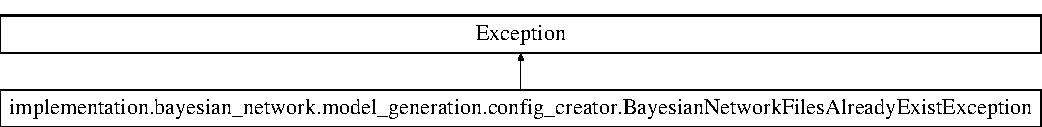
\includegraphics[height=1.712538cm]{classimplementation_1_1bayesian__network_1_1model__generation_1_1config__creator_1_1_bayesian_neaa9550024351ca391a952f36bc1cef38}
\end{center}
\end{figure}


The documentation for this class was generated from the following file\+:\begin{DoxyCompactItemize}
\item 
implementation/bayesian\+\_\+network/model\+\_\+generation/\hyperlink{config__creator_8py}{config\+\_\+creator.\+py}\end{DoxyCompactItemize}

\hypertarget{classimplementation_1_1actor__situation__class__detection_1_1bayesian__network__id__selection_1_40d4bcf4976295a8eb746907b1105fdb}{}\doxysection{implementation.\+actor\+\_\+situation\+\_\+class\+\_\+detection.\+bayesian\+\_\+network\+\_\+id\+\_\+selection.\+bayesian\+\_\+network\+\_\+id\+\_\+selector.\+Bayesian\+Network\+Id\+Selector Class Reference}
\label{classimplementation_1_1actor__situation__class__detection_1_1bayesian__network__id__selection_1_40d4bcf4976295a8eb746907b1105fdb}\index{implementation.actor\_situation\_class\_detection.bayesian\_network\_id\_selection.bayesian\_network\_id\_selector.BayesianNetworkIdSelector@{implementation.actor\_situation\_class\_detection.bayesian\_network\_id\_selection.bayesian\_network\_id\_selector.BayesianNetworkIdSelector}}
Inheritance diagram for implementation.\+actor\+\_\+situation\+\_\+class\+\_\+detection.\+bayesian\+\_\+network\+\_\+id\+\_\+selection.\+bayesian\+\_\+network\+\_\+id\+\_\+selector.\+Bayesian\+Network\+Id\+Selector\+:\begin{figure}[H]
\begin{center}
\leavevmode
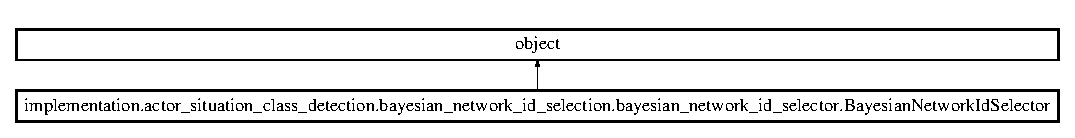
\includegraphics[height=1.407035cm]{classimplementation_1_1actor__situation__class__detection_1_1bayesian__network__id__selection_1_40d4bcf4976295a8eb746907b1105fdb}
\end{center}
\end{figure}
\doxysubsection*{Public Member Functions}
\begin{DoxyCompactItemize}
\item 
def \mbox{\hyperlink{classimplementation_1_1actor__situation__class__detection_1_1bayesian__network__id__selection_1_40d4bcf4976295a8eb746907b1105fdb_abf4d1c5395de40af3b9b1289314420d8}{\+\_\+\+\_\+init\+\_\+\+\_\+}} (self, \mbox{\hyperlink{classimplementation_1_1actor__situation__class__detection_1_1vehicle__actor__wrapper_1_1_vehicle_actor_wrapper}{Vehicle\+Actor\+Wrapper}} \mbox{\hyperlink{classimplementation_1_1actor__situation__class__detection_1_1bayesian__network__id__selection_1_40d4bcf4976295a8eb746907b1105fdb_ab504feda1df4eab9286dab437789804e}{wrapped\+\_\+hero\+\_\+vehicle}}, \mbox{\hyperlink{classimplementation_1_1actor__situation__class__detection_1_1situation__class_1_1_situation_class}{Situation\+Class}} \mbox{\hyperlink{classimplementation_1_1actor__situation__class__detection_1_1bayesian__network__id__selection_1_40d4bcf4976295a8eb746907b1105fdb_a5b964cebad74e374b922eef8623d03f4}{hero\+\_\+situation\+\_\+class}}, List\mbox{[}\char`\"{}Vehicle\+Actor\+Wrapper\char`\"{}\mbox{]} wrapped\+\_\+other\+\_\+vehicles, carla.\+Map carla\+\_\+map, carla.\+Debug\+Helper carla\+\_\+debug\+\_\+helper)
\item 
List\mbox{[}\char`\"{}Vehicle\+Dependent\+B\+N\+Id\char`\"{}\mbox{]} \mbox{\hyperlink{classimplementation_1_1actor__situation__class__detection_1_1bayesian__network__id__selection_1_40d4bcf4976295a8eb746907b1105fdb_a7f63374e24b32422721ab02741eda188}{get\+\_\+vehicle\+\_\+dependent\+\_\+bn\+\_\+ids}} (self)
\end{DoxyCompactItemize}
\doxysubsection*{Public Attributes}
\begin{DoxyCompactItemize}
\item 
\mbox{\hyperlink{classimplementation_1_1actor__situation__class__detection_1_1bayesian__network__id__selection_1_40d4bcf4976295a8eb746907b1105fdb_ab504feda1df4eab9286dab437789804e}{wrapped\+\_\+hero\+\_\+vehicle}}
\item 
\mbox{\hyperlink{classimplementation_1_1actor__situation__class__detection_1_1bayesian__network__id__selection_1_40d4bcf4976295a8eb746907b1105fdb_a5b964cebad74e374b922eef8623d03f4}{hero\+\_\+situation\+\_\+class}}
\item 
\mbox{\hyperlink{classimplementation_1_1actor__situation__class__detection_1_1bayesian__network__id__selection_1_40d4bcf4976295a8eb746907b1105fdb_a981123d4f9f47276790da04bac552810}{wrapped\+\_\+other\+\_\+vehicles}}
\end{DoxyCompactItemize}


\doxysubsection{Constructor \& Destructor Documentation}
\mbox{\Hypertarget{classimplementation_1_1actor__situation__class__detection_1_1bayesian__network__id__selection_1_40d4bcf4976295a8eb746907b1105fdb_abf4d1c5395de40af3b9b1289314420d8}\label{classimplementation_1_1actor__situation__class__detection_1_1bayesian__network__id__selection_1_40d4bcf4976295a8eb746907b1105fdb_abf4d1c5395de40af3b9b1289314420d8}} 
\index{implementation.actor\_situation\_class\_detection.bayesian\_network\_id\_selection.bayesian\_network\_id\_selector.BayesianNetworkIdSelector@{implementation.actor\_situation\_class\_detection.bayesian\_network\_id\_selection.bayesian\_network\_id\_selector.BayesianNetworkIdSelector}!\_\_init\_\_@{\_\_init\_\_}}
\index{\_\_init\_\_@{\_\_init\_\_}!implementation.actor\_situation\_class\_detection.bayesian\_network\_id\_selection.bayesian\_network\_id\_selector.BayesianNetworkIdSelector@{implementation.actor\_situation\_class\_detection.bayesian\_network\_id\_selection.bayesian\_network\_id\_selector.BayesianNetworkIdSelector}}
\doxysubsubsection{\texorpdfstring{\_\_init\_\_()}{\_\_init\_\_()}}
{\footnotesize\ttfamily def implementation.\+actor\+\_\+situation\+\_\+class\+\_\+detection.\+bayesian\+\_\+network\+\_\+id\+\_\+selection.\+bayesian\+\_\+network\+\_\+id\+\_\+selector.\+Bayesian\+Network\+Id\+Selector.\+\_\+\+\_\+init\+\_\+\+\_\+ (\begin{DoxyParamCaption}\item[{}]{self,  }\item[{\mbox{\hyperlink{classimplementation_1_1actor__situation__class__detection_1_1vehicle__actor__wrapper_1_1_vehicle_actor_wrapper}{Vehicle\+Actor\+Wrapper}}}]{wrapped\+\_\+hero\+\_\+vehicle,  }\item[{\mbox{\hyperlink{classimplementation_1_1actor__situation__class__detection_1_1situation__class_1_1_situation_class}{Situation\+Class}}}]{hero\+\_\+situation\+\_\+class,  }\item[{List\mbox{[}\char`\"{}Vehicle\+Actor\+Wrapper\char`\"{}\mbox{]}}]{wrapped\+\_\+other\+\_\+vehicles,  }\item[{carla.\+Map}]{carla\+\_\+map,  }\item[{carla.\+Debug\+Helper}]{carla\+\_\+debug\+\_\+helper }\end{DoxyParamCaption})}



\doxysubsection{Member Function Documentation}
\mbox{\Hypertarget{classimplementation_1_1actor__situation__class__detection_1_1bayesian__network__id__selection_1_40d4bcf4976295a8eb746907b1105fdb_a7f63374e24b32422721ab02741eda188}\label{classimplementation_1_1actor__situation__class__detection_1_1bayesian__network__id__selection_1_40d4bcf4976295a8eb746907b1105fdb_a7f63374e24b32422721ab02741eda188}} 
\index{implementation.actor\_situation\_class\_detection.bayesian\_network\_id\_selection.bayesian\_network\_id\_selector.BayesianNetworkIdSelector@{implementation.actor\_situation\_class\_detection.bayesian\_network\_id\_selection.bayesian\_network\_id\_selector.BayesianNetworkIdSelector}!get\_vehicle\_dependent\_bn\_ids@{get\_vehicle\_dependent\_bn\_ids}}
\index{get\_vehicle\_dependent\_bn\_ids@{get\_vehicle\_dependent\_bn\_ids}!implementation.actor\_situation\_class\_detection.bayesian\_network\_id\_selection.bayesian\_network\_id\_selector.BayesianNetworkIdSelector@{implementation.actor\_situation\_class\_detection.bayesian\_network\_id\_selection.bayesian\_network\_id\_selector.BayesianNetworkIdSelector}}
\doxysubsubsection{\texorpdfstring{get\_vehicle\_dependent\_bn\_ids()}{get\_vehicle\_dependent\_bn\_ids()}}
{\footnotesize\ttfamily  List\mbox{[}\char`\"{}Vehicle\+Dependent\+B\+N\+Id\char`\"{}\mbox{]} implementation.\+actor\+\_\+situation\+\_\+class\+\_\+detection.\+bayesian\+\_\+network\+\_\+id\+\_\+selection.\+bayesian\+\_\+network\+\_\+id\+\_\+selector.\+Bayesian\+Network\+Id\+Selector.\+get\+\_\+vehicle\+\_\+dependent\+\_\+bn\+\_\+ids (\begin{DoxyParamCaption}\item[{}]{self }\end{DoxyParamCaption})}

\begin{DoxyVerb}This method first checks the current situation class the hero vehicle is in.
Dependent on the active situation class, a specific bayesian network id selector object is created for obtaining
the corresponding bayesian network ids for each vehicle.
:return: List of VehicleDependentBNId objects
\end{DoxyVerb}
 

\doxysubsection{Member Data Documentation}
\mbox{\Hypertarget{classimplementation_1_1actor__situation__class__detection_1_1bayesian__network__id__selection_1_40d4bcf4976295a8eb746907b1105fdb_a5b964cebad74e374b922eef8623d03f4}\label{classimplementation_1_1actor__situation__class__detection_1_1bayesian__network__id__selection_1_40d4bcf4976295a8eb746907b1105fdb_a5b964cebad74e374b922eef8623d03f4}} 
\index{implementation.actor\_situation\_class\_detection.bayesian\_network\_id\_selection.bayesian\_network\_id\_selector.BayesianNetworkIdSelector@{implementation.actor\_situation\_class\_detection.bayesian\_network\_id\_selection.bayesian\_network\_id\_selector.BayesianNetworkIdSelector}!hero\_situation\_class@{hero\_situation\_class}}
\index{hero\_situation\_class@{hero\_situation\_class}!implementation.actor\_situation\_class\_detection.bayesian\_network\_id\_selection.bayesian\_network\_id\_selector.BayesianNetworkIdSelector@{implementation.actor\_situation\_class\_detection.bayesian\_network\_id\_selection.bayesian\_network\_id\_selector.BayesianNetworkIdSelector}}
\doxysubsubsection{\texorpdfstring{hero\_situation\_class}{hero\_situation\_class}}
{\footnotesize\ttfamily implementation.\+actor\+\_\+situation\+\_\+class\+\_\+detection.\+bayesian\+\_\+network\+\_\+id\+\_\+selection.\+bayesian\+\_\+network\+\_\+id\+\_\+selector.\+Bayesian\+Network\+Id\+Selector.\+hero\+\_\+situation\+\_\+class}

\mbox{\Hypertarget{classimplementation_1_1actor__situation__class__detection_1_1bayesian__network__id__selection_1_40d4bcf4976295a8eb746907b1105fdb_ab504feda1df4eab9286dab437789804e}\label{classimplementation_1_1actor__situation__class__detection_1_1bayesian__network__id__selection_1_40d4bcf4976295a8eb746907b1105fdb_ab504feda1df4eab9286dab437789804e}} 
\index{implementation.actor\_situation\_class\_detection.bayesian\_network\_id\_selection.bayesian\_network\_id\_selector.BayesianNetworkIdSelector@{implementation.actor\_situation\_class\_detection.bayesian\_network\_id\_selection.bayesian\_network\_id\_selector.BayesianNetworkIdSelector}!wrapped\_hero\_vehicle@{wrapped\_hero\_vehicle}}
\index{wrapped\_hero\_vehicle@{wrapped\_hero\_vehicle}!implementation.actor\_situation\_class\_detection.bayesian\_network\_id\_selection.bayesian\_network\_id\_selector.BayesianNetworkIdSelector@{implementation.actor\_situation\_class\_detection.bayesian\_network\_id\_selection.bayesian\_network\_id\_selector.BayesianNetworkIdSelector}}
\doxysubsubsection{\texorpdfstring{wrapped\_hero\_vehicle}{wrapped\_hero\_vehicle}}
{\footnotesize\ttfamily implementation.\+actor\+\_\+situation\+\_\+class\+\_\+detection.\+bayesian\+\_\+network\+\_\+id\+\_\+selection.\+bayesian\+\_\+network\+\_\+id\+\_\+selector.\+Bayesian\+Network\+Id\+Selector.\+wrapped\+\_\+hero\+\_\+vehicle}

\mbox{\Hypertarget{classimplementation_1_1actor__situation__class__detection_1_1bayesian__network__id__selection_1_40d4bcf4976295a8eb746907b1105fdb_a981123d4f9f47276790da04bac552810}\label{classimplementation_1_1actor__situation__class__detection_1_1bayesian__network__id__selection_1_40d4bcf4976295a8eb746907b1105fdb_a981123d4f9f47276790da04bac552810}} 
\index{implementation.actor\_situation\_class\_detection.bayesian\_network\_id\_selection.bayesian\_network\_id\_selector.BayesianNetworkIdSelector@{implementation.actor\_situation\_class\_detection.bayesian\_network\_id\_selection.bayesian\_network\_id\_selector.BayesianNetworkIdSelector}!wrapped\_other\_vehicles@{wrapped\_other\_vehicles}}
\index{wrapped\_other\_vehicles@{wrapped\_other\_vehicles}!implementation.actor\_situation\_class\_detection.bayesian\_network\_id\_selection.bayesian\_network\_id\_selector.BayesianNetworkIdSelector@{implementation.actor\_situation\_class\_detection.bayesian\_network\_id\_selection.bayesian\_network\_id\_selector.BayesianNetworkIdSelector}}
\doxysubsubsection{\texorpdfstring{wrapped\_other\_vehicles}{wrapped\_other\_vehicles}}
{\footnotesize\ttfamily implementation.\+actor\+\_\+situation\+\_\+class\+\_\+detection.\+bayesian\+\_\+network\+\_\+id\+\_\+selection.\+bayesian\+\_\+network\+\_\+id\+\_\+selector.\+Bayesian\+Network\+Id\+Selector.\+wrapped\+\_\+other\+\_\+vehicles}



The documentation for this class was generated from the following file\+:\begin{DoxyCompactItemize}
\item 
implementation/actor\+\_\+situation\+\_\+class\+\_\+detection/bayesian\+\_\+network\+\_\+id\+\_\+selection/\mbox{\hyperlink{bayesian__network__id__selector_8py}{bayesian\+\_\+network\+\_\+id\+\_\+selector.\+py}}\end{DoxyCompactItemize}

\hypertarget{classimplementation_1_1bayesian__network_1_1inference_1_1inference_1_1_bayesian_network_inference}{}\section{implementation.\+bayesian\+\_\+network.\+inference.\+inference.\+Bayesian\+Network\+Inference Class Reference}
\label{classimplementation_1_1bayesian__network_1_1inference_1_1inference_1_1_bayesian_network_inference}\index{implementation.\+bayesian\+\_\+network.\+inference.\+inference.\+Bayesian\+Network\+Inference@{implementation.\+bayesian\+\_\+network.\+inference.\+inference.\+Bayesian\+Network\+Inference}}
\subsection*{Public Member Functions}
\begin{DoxyCompactItemize}
\item 
def \hyperlink{classimplementation_1_1bayesian__network_1_1inference_1_1inference_1_1_bayesian_network_inference_a4c5aac13eccb5c4b0c5e7f7d3429cc13}{bn\+\_\+inferences\+\_\+for\+\_\+vehicles}
\end{DoxyCompactItemize}


\subsection{Detailed Description}
\begin{DoxyVerb}Performs the Bayesian network inference for all given Bayesian models and input features.\end{DoxyVerb}
 

\subsection{Member Function Documentation}
\mbox{\Hypertarget{classimplementation_1_1bayesian__network_1_1inference_1_1inference_1_1_bayesian_network_inference_a4c5aac13eccb5c4b0c5e7f7d3429cc13}\label{classimplementation_1_1bayesian__network_1_1inference_1_1inference_1_1_bayesian_network_inference_a4c5aac13eccb5c4b0c5e7f7d3429cc13}} 
\index{implementation\+::bayesian\+\_\+network\+::inference\+::inference\+::\+Bayesian\+Network\+Inference@{implementation\+::bayesian\+\_\+network\+::inference\+::inference\+::\+Bayesian\+Network\+Inference}!bn\+\_\+inferences\+\_\+for\+\_\+vehicles@{bn\+\_\+inferences\+\_\+for\+\_\+vehicles}}
\index{bn\+\_\+inferences\+\_\+for\+\_\+vehicles@{bn\+\_\+inferences\+\_\+for\+\_\+vehicles}!implementation\+::bayesian\+\_\+network\+::inference\+::inference\+::\+Bayesian\+Network\+Inference@{implementation\+::bayesian\+\_\+network\+::inference\+::inference\+::\+Bayesian\+Network\+Inference}}
\subsubsection{\texorpdfstring{bn\+\_\+inferences\+\_\+for\+\_\+vehicles()}{bn\_inferences\_for\_vehicles()}}
{\footnotesize\ttfamily def implementation.\+bayesian\+\_\+network.\+inference.\+inference.\+Bayesian\+Network\+Inference.\+bn\+\_\+inferences\+\_\+for\+\_\+vehicles (\begin{DoxyParamCaption}\item[{}]{self,  }\item[{}]{bayesian\+\_\+network\+\_\+data }\end{DoxyParamCaption})}



The documentation for this class was generated from the following file\+:\begin{DoxyCompactItemize}
\item 
implementation/bayesian\+\_\+network/inference/\hyperlink{inference_8py}{inference.\+py}\end{DoxyCompactItemize}

\hypertarget{classimplementation_1_1bayesian__network_1_1inference_1_1interfaces_1_1_bayesian_network_input_feature_data}{}\section{implementation.\+bayesian\+\_\+network.\+inference.\+interfaces.\+Bayesian\+Network\+Input\+Feature\+Data Class Reference}
\label{classimplementation_1_1bayesian__network_1_1inference_1_1interfaces_1_1_bayesian_network_input_feature_data}\index{implementation.\+bayesian\+\_\+network.\+inference.\+interfaces.\+Bayesian\+Network\+Input\+Feature\+Data@{implementation.\+bayesian\+\_\+network.\+inference.\+interfaces.\+Bayesian\+Network\+Input\+Feature\+Data}}
\subsection*{Static Public Member Functions}
\begin{DoxyCompactItemize}
\item 
def \hyperlink{classimplementation_1_1bayesian__network_1_1inference_1_1interfaces_1_1_bayesian_network_input_feature_data_a23717b9e24d7048b1af3425c7e824432}{set\+\_\+environment}
\item 
def \hyperlink{classimplementation_1_1bayesian__network_1_1inference_1_1interfaces_1_1_bayesian_network_input_feature_data_a159d5e2bf1018e48846f577c7cab8b67}{set\+\_\+map}
\end{DoxyCompactItemize}


\subsection{Detailed Description}
\begin{DoxyVerb}Data class that is used as input for the creation of the Bayesian network's specific input feature data classes
that are used in the Bayesian network configurations.
(Python dataclasses.dataclass object.)

Attributes
----------
vehicle_id : str
    Identifier of the respective vehicle.
vehicle : EgoVehicle,  OtherVehicle
    Vehicle object for the given vehicle
bayesian_network_id : Optional[str]
    Identifier for the Bayesian network that shall be used for the inference. Will only be set if the inference
    will be performed for this specific vehicle. (The default value is None.)

environment : Environment
    (Class attribute) Environment object, containing information about the weather etc
map : Map
    (Class attribute) Map object for the current world which is the access point for the topology
\end{DoxyVerb}
 

\subsection{Member Function Documentation}
\mbox{\Hypertarget{classimplementation_1_1bayesian__network_1_1inference_1_1interfaces_1_1_bayesian_network_input_feature_data_a23717b9e24d7048b1af3425c7e824432}\label{classimplementation_1_1bayesian__network_1_1inference_1_1interfaces_1_1_bayesian_network_input_feature_data_a23717b9e24d7048b1af3425c7e824432}} 
\index{implementation\+::bayesian\+\_\+network\+::inference\+::interfaces\+::\+Bayesian\+Network\+Input\+Feature\+Data@{implementation\+::bayesian\+\_\+network\+::inference\+::interfaces\+::\+Bayesian\+Network\+Input\+Feature\+Data}!set\+\_\+environment@{set\+\_\+environment}}
\index{set\+\_\+environment@{set\+\_\+environment}!implementation\+::bayesian\+\_\+network\+::inference\+::interfaces\+::\+Bayesian\+Network\+Input\+Feature\+Data@{implementation\+::bayesian\+\_\+network\+::inference\+::interfaces\+::\+Bayesian\+Network\+Input\+Feature\+Data}}
\subsubsection{\texorpdfstring{set\+\_\+environment()}{set\_environment()}}
{\footnotesize\ttfamily def implementation.\+bayesian\+\_\+network.\+inference.\+interfaces.\+Bayesian\+Network\+Input\+Feature\+Data.\+set\+\_\+environment (\begin{DoxyParamCaption}\item[{}]{environment }\end{DoxyParamCaption})\hspace{0.3cm}{\ttfamily [static]}}

\mbox{\Hypertarget{classimplementation_1_1bayesian__network_1_1inference_1_1interfaces_1_1_bayesian_network_input_feature_data_a159d5e2bf1018e48846f577c7cab8b67}\label{classimplementation_1_1bayesian__network_1_1inference_1_1interfaces_1_1_bayesian_network_input_feature_data_a159d5e2bf1018e48846f577c7cab8b67}} 
\index{implementation\+::bayesian\+\_\+network\+::inference\+::interfaces\+::\+Bayesian\+Network\+Input\+Feature\+Data@{implementation\+::bayesian\+\_\+network\+::inference\+::interfaces\+::\+Bayesian\+Network\+Input\+Feature\+Data}!set\+\_\+map@{set\+\_\+map}}
\index{set\+\_\+map@{set\+\_\+map}!implementation\+::bayesian\+\_\+network\+::inference\+::interfaces\+::\+Bayesian\+Network\+Input\+Feature\+Data@{implementation\+::bayesian\+\_\+network\+::inference\+::interfaces\+::\+Bayesian\+Network\+Input\+Feature\+Data}}
\subsubsection{\texorpdfstring{set\+\_\+map()}{set\_map()}}
{\footnotesize\ttfamily def implementation.\+bayesian\+\_\+network.\+inference.\+interfaces.\+Bayesian\+Network\+Input\+Feature\+Data.\+set\+\_\+map (\begin{DoxyParamCaption}\item[{}]{map }\end{DoxyParamCaption})\hspace{0.3cm}{\ttfamily [static]}}



The documentation for this class was generated from the following file\+:\begin{DoxyCompactItemize}
\item 
implementation/bayesian\+\_\+network/inference/\hyperlink{interfaces_8py}{interfaces.\+py}\end{DoxyCompactItemize}

\hypertarget{classimplementation_1_1bayesian__network_1_1inference_1_1interfaces_1_1_bayesian_network_output}{}\doxysection{implementation.\+bayesian\+\_\+network.\+inference.\+interfaces.\+Bayesian\+Network\+Output Class Reference}
\label{classimplementation_1_1bayesian__network_1_1inference_1_1interfaces_1_1_bayesian_network_output}\index{implementation.bayesian\_network.inference.interfaces.BayesianNetworkOutput@{implementation.bayesian\_network.inference.interfaces.BayesianNetworkOutput}}
\doxysubsection*{Public Member Functions}
\begin{DoxyCompactItemize}
\item 
str \mbox{\hyperlink{classimplementation_1_1bayesian__network_1_1inference_1_1interfaces_1_1_bayesian_network_output_a32453a2920d9adb2fd61d7cf7957e260}{\+\_\+\+\_\+str\+\_\+\+\_\+}} (self)
\end{DoxyCompactItemize}


\doxysubsection{Detailed Description}
\begin{DoxyVerb}This data class describes the output after a Bayesian network inference for a specific vehicle. For given output
nodes the infered values and their states are collected in here.
(Python dataclasses.dataclass object.)

Attributes
----------
vehicle_id : str
    Identifier of the respective vehicle.
vehicle_situation_state_id : Optional[BayesianNetId]
    State of the vehicle relative to the ego vehicle and its situation class.  (The default value is None.)
    (E.g. indicating the state of being a front vehicle in a lane following situation.)
bayesian_network_id : Optional[str]
    Identifier for the Bayesian network that was used for the inference.
output_nodes : List[Node]
    List of the defined output nodes for this Bayesian network. The infered node values and states are saved in
    here.
\end{DoxyVerb}
 

\doxysubsection{Member Function Documentation}
\mbox{\Hypertarget{classimplementation_1_1bayesian__network_1_1inference_1_1interfaces_1_1_bayesian_network_output_a32453a2920d9adb2fd61d7cf7957e260}\label{classimplementation_1_1bayesian__network_1_1inference_1_1interfaces_1_1_bayesian_network_output_a32453a2920d9adb2fd61d7cf7957e260}} 
\index{implementation.bayesian\_network.inference.interfaces.BayesianNetworkOutput@{implementation.bayesian\_network.inference.interfaces.BayesianNetworkOutput}!\_\_str\_\_@{\_\_str\_\_}}
\index{\_\_str\_\_@{\_\_str\_\_}!implementation.bayesian\_network.inference.interfaces.BayesianNetworkOutput@{implementation.bayesian\_network.inference.interfaces.BayesianNetworkOutput}}
\doxysubsubsection{\texorpdfstring{\_\_str\_\_()}{\_\_str\_\_()}}
{\footnotesize\ttfamily  str implementation.\+bayesian\+\_\+network.\+inference.\+interfaces.\+Bayesian\+Network\+Output.\+\_\+\+\_\+str\+\_\+\+\_\+ (\begin{DoxyParamCaption}\item[{}]{self }\end{DoxyParamCaption})}



The documentation for this class was generated from the following file\+:\begin{DoxyCompactItemize}
\item 
implementation/bayesian\+\_\+network/inference/\mbox{\hyperlink{interfaces_8py}{interfaces.\+py}}\end{DoxyCompactItemize}

\hypertarget{classimplementation_1_1sinadra__configuration__parameters_1_1_behavior_type}{}\section{implementation.\+sinadra\+\_\+configuration\+\_\+parameters.\+Behavior\+Type Class Reference}
\label{classimplementation_1_1sinadra__configuration__parameters_1_1_behavior_type}\index{implementation.\+sinadra\+\_\+configuration\+\_\+parameters.\+Behavior\+Type@{implementation.\+sinadra\+\_\+configuration\+\_\+parameters.\+Behavior\+Type}}


BN Inference parameters.  


Inheritance diagram for implementation.\+sinadra\+\_\+configuration\+\_\+parameters.\+Behavior\+Type\+:\begin{figure}[H]
\begin{center}
\leavevmode
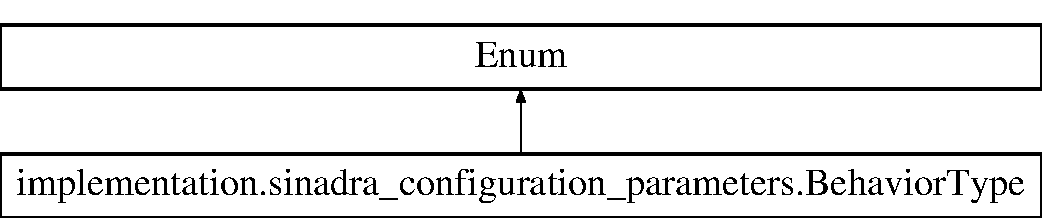
\includegraphics[height=2.000000cm]{classimplementation_1_1sinadra__configuration__parameters_1_1_behavior_type}
\end{center}
\end{figure}
\subsection*{Static Public Attributes}
\begin{DoxyCompactItemize}
\item 
\hyperlink{namespaceimplementation_1_1sinadra__configuration__parameters_a1053d4f6819fcba166f4cf443ab0123d}{int} \hyperlink{classimplementation_1_1sinadra__configuration__parameters_1_1_behavior_type_a067bea59d67bb5900eb8dbb35ad22deb}{Braking} = 1
\item 
\hyperlink{namespaceimplementation_1_1sinadra__configuration__parameters_a1053d4f6819fcba166f4cf443ab0123d}{int} \hyperlink{classimplementation_1_1sinadra__configuration__parameters_1_1_behavior_type_ac05e3aaf6d0f49dc7baca5efdd5f89e4}{Lane\+Change\+To\+Left} = 2
\item 
\hyperlink{namespaceimplementation_1_1sinadra__configuration__parameters_a1053d4f6819fcba166f4cf443ab0123d}{int} \hyperlink{classimplementation_1_1sinadra__configuration__parameters_1_1_behavior_type_a5a1cb89e84054858ec7dc07945b526bf}{Lane\+Change\+To\+Right} = 3
\end{DoxyCompactItemize}


\subsection{Detailed Description}
BN Inference parameters. 

BN \& Risk Computation parameters 

\subsection{Member Data Documentation}
\mbox{\Hypertarget{classimplementation_1_1sinadra__configuration__parameters_1_1_behavior_type_a067bea59d67bb5900eb8dbb35ad22deb}\label{classimplementation_1_1sinadra__configuration__parameters_1_1_behavior_type_a067bea59d67bb5900eb8dbb35ad22deb}} 
\index{implementation\+::sinadra\+\_\+configuration\+\_\+parameters\+::\+Behavior\+Type@{implementation\+::sinadra\+\_\+configuration\+\_\+parameters\+::\+Behavior\+Type}!Braking@{Braking}}
\index{Braking@{Braking}!implementation\+::sinadra\+\_\+configuration\+\_\+parameters\+::\+Behavior\+Type@{implementation\+::sinadra\+\_\+configuration\+\_\+parameters\+::\+Behavior\+Type}}
\subsubsection{\texorpdfstring{Braking}{Braking}}
{\footnotesize\ttfamily \hyperlink{namespaceimplementation_1_1sinadra__configuration__parameters_a1053d4f6819fcba166f4cf443ab0123d}{int} implementation.\+sinadra\+\_\+configuration\+\_\+parameters.\+Behavior\+Type.\+Braking = 1\hspace{0.3cm}{\ttfamily [static]}}

\mbox{\Hypertarget{classimplementation_1_1sinadra__configuration__parameters_1_1_behavior_type_ac05e3aaf6d0f49dc7baca5efdd5f89e4}\label{classimplementation_1_1sinadra__configuration__parameters_1_1_behavior_type_ac05e3aaf6d0f49dc7baca5efdd5f89e4}} 
\index{implementation\+::sinadra\+\_\+configuration\+\_\+parameters\+::\+Behavior\+Type@{implementation\+::sinadra\+\_\+configuration\+\_\+parameters\+::\+Behavior\+Type}!Lane\+Change\+To\+Left@{Lane\+Change\+To\+Left}}
\index{Lane\+Change\+To\+Left@{Lane\+Change\+To\+Left}!implementation\+::sinadra\+\_\+configuration\+\_\+parameters\+::\+Behavior\+Type@{implementation\+::sinadra\+\_\+configuration\+\_\+parameters\+::\+Behavior\+Type}}
\subsubsection{\texorpdfstring{Lane\+Change\+To\+Left}{LaneChangeToLeft}}
{\footnotesize\ttfamily \hyperlink{namespaceimplementation_1_1sinadra__configuration__parameters_a1053d4f6819fcba166f4cf443ab0123d}{int} implementation.\+sinadra\+\_\+configuration\+\_\+parameters.\+Behavior\+Type.\+Lane\+Change\+To\+Left = 2\hspace{0.3cm}{\ttfamily [static]}}

\mbox{\Hypertarget{classimplementation_1_1sinadra__configuration__parameters_1_1_behavior_type_a5a1cb89e84054858ec7dc07945b526bf}\label{classimplementation_1_1sinadra__configuration__parameters_1_1_behavior_type_a5a1cb89e84054858ec7dc07945b526bf}} 
\index{implementation\+::sinadra\+\_\+configuration\+\_\+parameters\+::\+Behavior\+Type@{implementation\+::sinadra\+\_\+configuration\+\_\+parameters\+::\+Behavior\+Type}!Lane\+Change\+To\+Right@{Lane\+Change\+To\+Right}}
\index{Lane\+Change\+To\+Right@{Lane\+Change\+To\+Right}!implementation\+::sinadra\+\_\+configuration\+\_\+parameters\+::\+Behavior\+Type@{implementation\+::sinadra\+\_\+configuration\+\_\+parameters\+::\+Behavior\+Type}}
\subsubsection{\texorpdfstring{Lane\+Change\+To\+Right}{LaneChangeToRight}}
{\footnotesize\ttfamily \hyperlink{namespaceimplementation_1_1sinadra__configuration__parameters_a1053d4f6819fcba166f4cf443ab0123d}{int} implementation.\+sinadra\+\_\+configuration\+\_\+parameters.\+Behavior\+Type.\+Lane\+Change\+To\+Right = 3\hspace{0.3cm}{\ttfamily [static]}}



The documentation for this class was generated from the following file\+:\begin{DoxyCompactItemize}
\item 
implementation/\hyperlink{sinadra__configuration__parameters_8py}{sinadra\+\_\+configuration\+\_\+parameters.\+py}\end{DoxyCompactItemize}

\hypertarget{classimplementation_1_1data__model_1_1entity_1_1_bounding_box}{}\section{implementation.\+data\+\_\+model.\+entity.\+Bounding\+Box Class Reference}
\label{classimplementation_1_1data__model_1_1entity_1_1_bounding_box}\index{implementation.\+data\+\_\+model.\+entity.\+Bounding\+Box@{implementation.\+data\+\_\+model.\+entity.\+Bounding\+Box}}
\subsection*{Public Member Functions}
\begin{DoxyCompactItemize}
\item 
def \hyperlink{classimplementation_1_1data__model_1_1entity_1_1_bounding_box_aee06e03485e4ca7770eff56e30856cf2}{get\+\_\+middle\+\_\+points}
\item 
def \hyperlink{classimplementation_1_1data__model_1_1entity_1_1_bounding_box_af113a1cd36b743c1aeaf4274cd07933a}{get\+\_\+world\+\_\+vertices}
\item 
def \hyperlink{classimplementation_1_1data__model_1_1entity_1_1_bounding_box_afc64d90d6cccc29866992de2d6fdb7d7}{get\+\_\+local\+\_\+vertices} (self)
\end{DoxyCompactItemize}
\subsection*{Static Public Attributes}
\begin{DoxyCompactItemize}
\item 
\hyperlink{classimplementation_1_1data__model_1_1entity_1_1_bounding_box_a77a1e731c9cfef373c286b0ba2da7706}{Location}
\item 
\hyperlink{classimplementation_1_1data__model_1_1entity_1_1_bounding_box_a2260283c12eb6a02a4d6684cb4c44333}{Dimension}
\end{DoxyCompactItemize}


\subsection{Detailed Description}
\begin{DoxyVerb}Defines geometric properties of the entities as a simplified three dimensional bounding box.
(Python dataclasses.dataclass object.)

Attributes
----------
center : Location
    Represents the geometrical center of the bounding expressed in coordinates that refer to the coordinate
    system of the entity
dimension: Dimension
    Width, length and height of the bounding box
\end{DoxyVerb}
 

\subsection{Member Function Documentation}
\mbox{\Hypertarget{classimplementation_1_1data__model_1_1entity_1_1_bounding_box_afc64d90d6cccc29866992de2d6fdb7d7}\label{classimplementation_1_1data__model_1_1entity_1_1_bounding_box_afc64d90d6cccc29866992de2d6fdb7d7}} 
\index{implementation\+::data\+\_\+model\+::entity\+::\+Bounding\+Box@{implementation\+::data\+\_\+model\+::entity\+::\+Bounding\+Box}!get\+\_\+local\+\_\+vertices@{get\+\_\+local\+\_\+vertices}}
\index{get\+\_\+local\+\_\+vertices@{get\+\_\+local\+\_\+vertices}!implementation\+::data\+\_\+model\+::entity\+::\+Bounding\+Box@{implementation\+::data\+\_\+model\+::entity\+::\+Bounding\+Box}}
\subsubsection{\texorpdfstring{get\+\_\+local\+\_\+vertices()}{get\_local\_vertices()}}
{\footnotesize\ttfamily def implementation.\+data\+\_\+model.\+entity.\+Bounding\+Box.\+get\+\_\+local\+\_\+vertices (\begin{DoxyParamCaption}\item[{}]{self,  }\item[{}]{List,  }\item[{}]{Location }\end{DoxyParamCaption})}

\begin{DoxyVerb}Return the vertices of the bounding box using the local coordinate system of the object

Returns
-------
List[Location]
    List of Location objects representing a vertice using the objects local coordinates
\end{DoxyVerb}
 \mbox{\Hypertarget{classimplementation_1_1data__model_1_1entity_1_1_bounding_box_aee06e03485e4ca7770eff56e30856cf2}\label{classimplementation_1_1data__model_1_1entity_1_1_bounding_box_aee06e03485e4ca7770eff56e30856cf2}} 
\index{implementation\+::data\+\_\+model\+::entity\+::\+Bounding\+Box@{implementation\+::data\+\_\+model\+::entity\+::\+Bounding\+Box}!get\+\_\+middle\+\_\+points@{get\+\_\+middle\+\_\+points}}
\index{get\+\_\+middle\+\_\+points@{get\+\_\+middle\+\_\+points}!implementation\+::data\+\_\+model\+::entity\+::\+Bounding\+Box@{implementation\+::data\+\_\+model\+::entity\+::\+Bounding\+Box}}
\subsubsection{\texorpdfstring{get\+\_\+middle\+\_\+points()}{get\_middle\_points()}}
{\footnotesize\ttfamily def implementation.\+data\+\_\+model.\+entity.\+Bounding\+Box.\+get\+\_\+middle\+\_\+points (\begin{DoxyParamCaption}\item[{}]{self,  }\item[{}]{world\+\_\+position }\end{DoxyParamCaption})}

\mbox{\Hypertarget{classimplementation_1_1data__model_1_1entity_1_1_bounding_box_af113a1cd36b743c1aeaf4274cd07933a}\label{classimplementation_1_1data__model_1_1entity_1_1_bounding_box_af113a1cd36b743c1aeaf4274cd07933a}} 
\index{implementation\+::data\+\_\+model\+::entity\+::\+Bounding\+Box@{implementation\+::data\+\_\+model\+::entity\+::\+Bounding\+Box}!get\+\_\+world\+\_\+vertices@{get\+\_\+world\+\_\+vertices}}
\index{get\+\_\+world\+\_\+vertices@{get\+\_\+world\+\_\+vertices}!implementation\+::data\+\_\+model\+::entity\+::\+Bounding\+Box@{implementation\+::data\+\_\+model\+::entity\+::\+Bounding\+Box}}
\subsubsection{\texorpdfstring{get\+\_\+world\+\_\+vertices()}{get\_world\_vertices()}}
{\footnotesize\ttfamily def implementation.\+data\+\_\+model.\+entity.\+Bounding\+Box.\+get\+\_\+world\+\_\+vertices (\begin{DoxyParamCaption}\item[{}]{self,  }\item[{}]{world\+\_\+position }\end{DoxyParamCaption})}



\subsection{Member Data Documentation}
\mbox{\Hypertarget{classimplementation_1_1data__model_1_1entity_1_1_bounding_box_a2260283c12eb6a02a4d6684cb4c44333}\label{classimplementation_1_1data__model_1_1entity_1_1_bounding_box_a2260283c12eb6a02a4d6684cb4c44333}} 
\index{implementation\+::data\+\_\+model\+::entity\+::\+Bounding\+Box@{implementation\+::data\+\_\+model\+::entity\+::\+Bounding\+Box}!Dimension@{Dimension}}
\index{Dimension@{Dimension}!implementation\+::data\+\_\+model\+::entity\+::\+Bounding\+Box@{implementation\+::data\+\_\+model\+::entity\+::\+Bounding\+Box}}
\subsubsection{\texorpdfstring{Dimension}{Dimension}}
{\footnotesize\ttfamily implementation.\+data\+\_\+model.\+entity.\+Bounding\+Box.\+Dimension\hspace{0.3cm}{\ttfamily [static]}}

\mbox{\Hypertarget{classimplementation_1_1data__model_1_1entity_1_1_bounding_box_a77a1e731c9cfef373c286b0ba2da7706}\label{classimplementation_1_1data__model_1_1entity_1_1_bounding_box_a77a1e731c9cfef373c286b0ba2da7706}} 
\index{implementation\+::data\+\_\+model\+::entity\+::\+Bounding\+Box@{implementation\+::data\+\_\+model\+::entity\+::\+Bounding\+Box}!Location@{Location}}
\index{Location@{Location}!implementation\+::data\+\_\+model\+::entity\+::\+Bounding\+Box@{implementation\+::data\+\_\+model\+::entity\+::\+Bounding\+Box}}
\subsubsection{\texorpdfstring{Location}{Location}}
{\footnotesize\ttfamily implementation.\+data\+\_\+model.\+entity.\+Bounding\+Box.\+Location\hspace{0.3cm}{\ttfamily [static]}}



The documentation for this class was generated from the following file\+:\begin{DoxyCompactItemize}
\item 
implementation/data\+\_\+model/\hyperlink{entity_8py}{entity.\+py}\end{DoxyCompactItemize}

\hypertarget{classimplementation_1_1manual__control_1_1_camera_manager}{}\section{implementation.\+manual\+\_\+control.\+Camera\+Manager Class Reference}
\label{classimplementation_1_1manual__control_1_1_camera_manager}\index{implementation.\+manual\+\_\+control.\+Camera\+Manager@{implementation.\+manual\+\_\+control.\+Camera\+Manager}}
Inheritance diagram for implementation.\+manual\+\_\+control.\+Camera\+Manager\+:\begin{figure}[H]
\begin{center}
\leavevmode
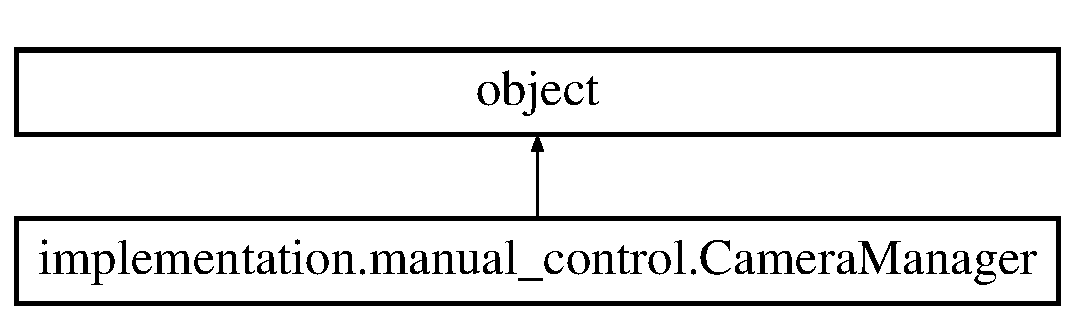
\includegraphics[height=2.000000cm]{classimplementation_1_1manual__control_1_1_camera_manager}
\end{center}
\end{figure}
\subsection*{Public Member Functions}
\begin{DoxyCompactItemize}
\item 
def \hyperlink{classimplementation_1_1manual__control_1_1_camera_manager_ab610af9a3694f6fc76ef1265a9f9d31d}{\+\_\+\+\_\+init\+\_\+\+\_\+} (self, parent\+\_\+actor, \hyperlink{classimplementation_1_1manual__control_1_1_camera_manager_a71d034dbe54b1daf605bf19dd4fe3520}{hud}, gamma\+\_\+correction)
\item 
def \hyperlink{classimplementation_1_1manual__control_1_1_camera_manager_a75e8e69628d124a50143fe09d9d50fb8}{toggle\+\_\+camera} (self)
\item 
def \hyperlink{classimplementation_1_1manual__control_1_1_camera_manager_a23111e5b5a28fe87fccb6bd853710429}{set\+\_\+sensor} (self, \hyperlink{classimplementation_1_1manual__control_1_1_camera_manager_a12aa1154aeb3e9dee255fcc207aaead7}{index}, notify=True, force\+\_\+respawn=False)
\item 
def \hyperlink{classimplementation_1_1manual__control_1_1_camera_manager_afc8a40102442781286b334ff42d28f99}{next\+\_\+sensor} (self)
\item 
def \hyperlink{classimplementation_1_1manual__control_1_1_camera_manager_aa872c41d5fa86ac5d0621b4582eee539}{toggle\+\_\+recording} (self)
\item 
def \hyperlink{classimplementation_1_1manual__control_1_1_camera_manager_a0ec5eb57da476b77c6ddb344dfa01fd5}{render} (self, display)
\end{DoxyCompactItemize}
\subsection*{Public Attributes}
\begin{DoxyCompactItemize}
\item 
\hyperlink{classimplementation_1_1manual__control_1_1_camera_manager_a08823c2f7684b1530c9bb28bb0d196b8}{sensor}
\item 
\hyperlink{classimplementation_1_1manual__control_1_1_camera_manager_a086798f2e17c6ccf3ae167167bb57ca7}{surface}
\item 
\hyperlink{classimplementation_1_1manual__control_1_1_camera_manager_a71d034dbe54b1daf605bf19dd4fe3520}{hud}
\item 
\hyperlink{classimplementation_1_1manual__control_1_1_camera_manager_a733748ba55b4692dfbefed8d6a3d0ff0}{recording}
\item 
\hyperlink{classimplementation_1_1manual__control_1_1_camera_manager_ad13f1309b723167fd9f621e1d787dc62}{transform\+\_\+index}
\item 
\hyperlink{classimplementation_1_1manual__control_1_1_camera_manager_a886aa6e9d84697920fc90c21e5a7d663}{sensors}
\item 
\hyperlink{classimplementation_1_1manual__control_1_1_camera_manager_a84274230a3a05611e594ef29f7394052}{lidar\+\_\+range}
\item 
\hyperlink{classimplementation_1_1manual__control_1_1_camera_manager_a12aa1154aeb3e9dee255fcc207aaead7}{index}
\end{DoxyCompactItemize}


\subsection{Constructor \& Destructor Documentation}
\mbox{\Hypertarget{classimplementation_1_1manual__control_1_1_camera_manager_ab610af9a3694f6fc76ef1265a9f9d31d}\label{classimplementation_1_1manual__control_1_1_camera_manager_ab610af9a3694f6fc76ef1265a9f9d31d}} 
\index{implementation\+::manual\+\_\+control\+::\+Camera\+Manager@{implementation\+::manual\+\_\+control\+::\+Camera\+Manager}!\+\_\+\+\_\+init\+\_\+\+\_\+@{\+\_\+\+\_\+init\+\_\+\+\_\+}}
\index{\+\_\+\+\_\+init\+\_\+\+\_\+@{\+\_\+\+\_\+init\+\_\+\+\_\+}!implementation\+::manual\+\_\+control\+::\+Camera\+Manager@{implementation\+::manual\+\_\+control\+::\+Camera\+Manager}}
\subsubsection{\texorpdfstring{\+\_\+\+\_\+init\+\_\+\+\_\+()}{\_\_init\_\_()}}
{\footnotesize\ttfamily def implementation.\+manual\+\_\+control.\+Camera\+Manager.\+\_\+\+\_\+init\+\_\+\+\_\+ (\begin{DoxyParamCaption}\item[{}]{self,  }\item[{}]{parent\+\_\+actor,  }\item[{}]{hud,  }\item[{}]{gamma\+\_\+correction }\end{DoxyParamCaption})}



\subsection{Member Function Documentation}
\mbox{\Hypertarget{classimplementation_1_1manual__control_1_1_camera_manager_afc8a40102442781286b334ff42d28f99}\label{classimplementation_1_1manual__control_1_1_camera_manager_afc8a40102442781286b334ff42d28f99}} 
\index{implementation\+::manual\+\_\+control\+::\+Camera\+Manager@{implementation\+::manual\+\_\+control\+::\+Camera\+Manager}!next\+\_\+sensor@{next\+\_\+sensor}}
\index{next\+\_\+sensor@{next\+\_\+sensor}!implementation\+::manual\+\_\+control\+::\+Camera\+Manager@{implementation\+::manual\+\_\+control\+::\+Camera\+Manager}}
\subsubsection{\texorpdfstring{next\+\_\+sensor()}{next\_sensor()}}
{\footnotesize\ttfamily def implementation.\+manual\+\_\+control.\+Camera\+Manager.\+next\+\_\+sensor (\begin{DoxyParamCaption}\item[{}]{self }\end{DoxyParamCaption})}

\mbox{\Hypertarget{classimplementation_1_1manual__control_1_1_camera_manager_a0ec5eb57da476b77c6ddb344dfa01fd5}\label{classimplementation_1_1manual__control_1_1_camera_manager_a0ec5eb57da476b77c6ddb344dfa01fd5}} 
\index{implementation\+::manual\+\_\+control\+::\+Camera\+Manager@{implementation\+::manual\+\_\+control\+::\+Camera\+Manager}!render@{render}}
\index{render@{render}!implementation\+::manual\+\_\+control\+::\+Camera\+Manager@{implementation\+::manual\+\_\+control\+::\+Camera\+Manager}}
\subsubsection{\texorpdfstring{render()}{render()}}
{\footnotesize\ttfamily def implementation.\+manual\+\_\+control.\+Camera\+Manager.\+render (\begin{DoxyParamCaption}\item[{}]{self,  }\item[{}]{display }\end{DoxyParamCaption})}

\mbox{\Hypertarget{classimplementation_1_1manual__control_1_1_camera_manager_a23111e5b5a28fe87fccb6bd853710429}\label{classimplementation_1_1manual__control_1_1_camera_manager_a23111e5b5a28fe87fccb6bd853710429}} 
\index{implementation\+::manual\+\_\+control\+::\+Camera\+Manager@{implementation\+::manual\+\_\+control\+::\+Camera\+Manager}!set\+\_\+sensor@{set\+\_\+sensor}}
\index{set\+\_\+sensor@{set\+\_\+sensor}!implementation\+::manual\+\_\+control\+::\+Camera\+Manager@{implementation\+::manual\+\_\+control\+::\+Camera\+Manager}}
\subsubsection{\texorpdfstring{set\+\_\+sensor()}{set\_sensor()}}
{\footnotesize\ttfamily def implementation.\+manual\+\_\+control.\+Camera\+Manager.\+set\+\_\+sensor (\begin{DoxyParamCaption}\item[{}]{self,  }\item[{}]{index,  }\item[{}]{notify = {\ttfamily True},  }\item[{}]{force\+\_\+respawn = {\ttfamily False} }\end{DoxyParamCaption})}

\mbox{\Hypertarget{classimplementation_1_1manual__control_1_1_camera_manager_a75e8e69628d124a50143fe09d9d50fb8}\label{classimplementation_1_1manual__control_1_1_camera_manager_a75e8e69628d124a50143fe09d9d50fb8}} 
\index{implementation\+::manual\+\_\+control\+::\+Camera\+Manager@{implementation\+::manual\+\_\+control\+::\+Camera\+Manager}!toggle\+\_\+camera@{toggle\+\_\+camera}}
\index{toggle\+\_\+camera@{toggle\+\_\+camera}!implementation\+::manual\+\_\+control\+::\+Camera\+Manager@{implementation\+::manual\+\_\+control\+::\+Camera\+Manager}}
\subsubsection{\texorpdfstring{toggle\+\_\+camera()}{toggle\_camera()}}
{\footnotesize\ttfamily def implementation.\+manual\+\_\+control.\+Camera\+Manager.\+toggle\+\_\+camera (\begin{DoxyParamCaption}\item[{}]{self }\end{DoxyParamCaption})}

\mbox{\Hypertarget{classimplementation_1_1manual__control_1_1_camera_manager_aa872c41d5fa86ac5d0621b4582eee539}\label{classimplementation_1_1manual__control_1_1_camera_manager_aa872c41d5fa86ac5d0621b4582eee539}} 
\index{implementation\+::manual\+\_\+control\+::\+Camera\+Manager@{implementation\+::manual\+\_\+control\+::\+Camera\+Manager}!toggle\+\_\+recording@{toggle\+\_\+recording}}
\index{toggle\+\_\+recording@{toggle\+\_\+recording}!implementation\+::manual\+\_\+control\+::\+Camera\+Manager@{implementation\+::manual\+\_\+control\+::\+Camera\+Manager}}
\subsubsection{\texorpdfstring{toggle\+\_\+recording()}{toggle\_recording()}}
{\footnotesize\ttfamily def implementation.\+manual\+\_\+control.\+Camera\+Manager.\+toggle\+\_\+recording (\begin{DoxyParamCaption}\item[{}]{self }\end{DoxyParamCaption})}



\subsection{Member Data Documentation}
\mbox{\Hypertarget{classimplementation_1_1manual__control_1_1_camera_manager_a71d034dbe54b1daf605bf19dd4fe3520}\label{classimplementation_1_1manual__control_1_1_camera_manager_a71d034dbe54b1daf605bf19dd4fe3520}} 
\index{implementation\+::manual\+\_\+control\+::\+Camera\+Manager@{implementation\+::manual\+\_\+control\+::\+Camera\+Manager}!hud@{hud}}
\index{hud@{hud}!implementation\+::manual\+\_\+control\+::\+Camera\+Manager@{implementation\+::manual\+\_\+control\+::\+Camera\+Manager}}
\subsubsection{\texorpdfstring{hud}{hud}}
{\footnotesize\ttfamily implementation.\+manual\+\_\+control.\+Camera\+Manager.\+hud}

\mbox{\Hypertarget{classimplementation_1_1manual__control_1_1_camera_manager_a12aa1154aeb3e9dee255fcc207aaead7}\label{classimplementation_1_1manual__control_1_1_camera_manager_a12aa1154aeb3e9dee255fcc207aaead7}} 
\index{implementation\+::manual\+\_\+control\+::\+Camera\+Manager@{implementation\+::manual\+\_\+control\+::\+Camera\+Manager}!index@{index}}
\index{index@{index}!implementation\+::manual\+\_\+control\+::\+Camera\+Manager@{implementation\+::manual\+\_\+control\+::\+Camera\+Manager}}
\subsubsection{\texorpdfstring{index}{index}}
{\footnotesize\ttfamily implementation.\+manual\+\_\+control.\+Camera\+Manager.\+index}

\mbox{\Hypertarget{classimplementation_1_1manual__control_1_1_camera_manager_a84274230a3a05611e594ef29f7394052}\label{classimplementation_1_1manual__control_1_1_camera_manager_a84274230a3a05611e594ef29f7394052}} 
\index{implementation\+::manual\+\_\+control\+::\+Camera\+Manager@{implementation\+::manual\+\_\+control\+::\+Camera\+Manager}!lidar\+\_\+range@{lidar\+\_\+range}}
\index{lidar\+\_\+range@{lidar\+\_\+range}!implementation\+::manual\+\_\+control\+::\+Camera\+Manager@{implementation\+::manual\+\_\+control\+::\+Camera\+Manager}}
\subsubsection{\texorpdfstring{lidar\+\_\+range}{lidar\_range}}
{\footnotesize\ttfamily implementation.\+manual\+\_\+control.\+Camera\+Manager.\+lidar\+\_\+range}

\mbox{\Hypertarget{classimplementation_1_1manual__control_1_1_camera_manager_a733748ba55b4692dfbefed8d6a3d0ff0}\label{classimplementation_1_1manual__control_1_1_camera_manager_a733748ba55b4692dfbefed8d6a3d0ff0}} 
\index{implementation\+::manual\+\_\+control\+::\+Camera\+Manager@{implementation\+::manual\+\_\+control\+::\+Camera\+Manager}!recording@{recording}}
\index{recording@{recording}!implementation\+::manual\+\_\+control\+::\+Camera\+Manager@{implementation\+::manual\+\_\+control\+::\+Camera\+Manager}}
\subsubsection{\texorpdfstring{recording}{recording}}
{\footnotesize\ttfamily implementation.\+manual\+\_\+control.\+Camera\+Manager.\+recording}

\mbox{\Hypertarget{classimplementation_1_1manual__control_1_1_camera_manager_a08823c2f7684b1530c9bb28bb0d196b8}\label{classimplementation_1_1manual__control_1_1_camera_manager_a08823c2f7684b1530c9bb28bb0d196b8}} 
\index{implementation\+::manual\+\_\+control\+::\+Camera\+Manager@{implementation\+::manual\+\_\+control\+::\+Camera\+Manager}!sensor@{sensor}}
\index{sensor@{sensor}!implementation\+::manual\+\_\+control\+::\+Camera\+Manager@{implementation\+::manual\+\_\+control\+::\+Camera\+Manager}}
\subsubsection{\texorpdfstring{sensor}{sensor}}
{\footnotesize\ttfamily implementation.\+manual\+\_\+control.\+Camera\+Manager.\+sensor}

\mbox{\Hypertarget{classimplementation_1_1manual__control_1_1_camera_manager_a886aa6e9d84697920fc90c21e5a7d663}\label{classimplementation_1_1manual__control_1_1_camera_manager_a886aa6e9d84697920fc90c21e5a7d663}} 
\index{implementation\+::manual\+\_\+control\+::\+Camera\+Manager@{implementation\+::manual\+\_\+control\+::\+Camera\+Manager}!sensors@{sensors}}
\index{sensors@{sensors}!implementation\+::manual\+\_\+control\+::\+Camera\+Manager@{implementation\+::manual\+\_\+control\+::\+Camera\+Manager}}
\subsubsection{\texorpdfstring{sensors}{sensors}}
{\footnotesize\ttfamily implementation.\+manual\+\_\+control.\+Camera\+Manager.\+sensors}

\mbox{\Hypertarget{classimplementation_1_1manual__control_1_1_camera_manager_a086798f2e17c6ccf3ae167167bb57ca7}\label{classimplementation_1_1manual__control_1_1_camera_manager_a086798f2e17c6ccf3ae167167bb57ca7}} 
\index{implementation\+::manual\+\_\+control\+::\+Camera\+Manager@{implementation\+::manual\+\_\+control\+::\+Camera\+Manager}!surface@{surface}}
\index{surface@{surface}!implementation\+::manual\+\_\+control\+::\+Camera\+Manager@{implementation\+::manual\+\_\+control\+::\+Camera\+Manager}}
\subsubsection{\texorpdfstring{surface}{surface}}
{\footnotesize\ttfamily implementation.\+manual\+\_\+control.\+Camera\+Manager.\+surface}

\mbox{\Hypertarget{classimplementation_1_1manual__control_1_1_camera_manager_ad13f1309b723167fd9f621e1d787dc62}\label{classimplementation_1_1manual__control_1_1_camera_manager_ad13f1309b723167fd9f621e1d787dc62}} 
\index{implementation\+::manual\+\_\+control\+::\+Camera\+Manager@{implementation\+::manual\+\_\+control\+::\+Camera\+Manager}!transform\+\_\+index@{transform\+\_\+index}}
\index{transform\+\_\+index@{transform\+\_\+index}!implementation\+::manual\+\_\+control\+::\+Camera\+Manager@{implementation\+::manual\+\_\+control\+::\+Camera\+Manager}}
\subsubsection{\texorpdfstring{transform\+\_\+index}{transform\_index}}
{\footnotesize\ttfamily implementation.\+manual\+\_\+control.\+Camera\+Manager.\+transform\+\_\+index}



The documentation for this class was generated from the following file\+:\begin{DoxyCompactItemize}
\item 
implementation/\hyperlink{manual__control_8py}{manual\+\_\+control.\+py}\end{DoxyCompactItemize}

\hypertarget{classimplementation_1_1simulators_1_1carla__simulator__controller_1_1_carla_simulator_controller}{}\section{implementation.\+simulators.\+carla\+\_\+simulator\+\_\+controller.\+Carla\+Simulator\+Controller Class Reference}
\label{classimplementation_1_1simulators_1_1carla__simulator__controller_1_1_carla_simulator_controller}\index{implementation.\+simulators.\+carla\+\_\+simulator\+\_\+controller.\+Carla\+Simulator\+Controller@{implementation.\+simulators.\+carla\+\_\+simulator\+\_\+controller.\+Carla\+Simulator\+Controller}}
Inheritance diagram for implementation.\+simulators.\+carla\+\_\+simulator\+\_\+controller.\+Carla\+Simulator\+Controller\+:\begin{figure}[H]
\begin{center}
\leavevmode
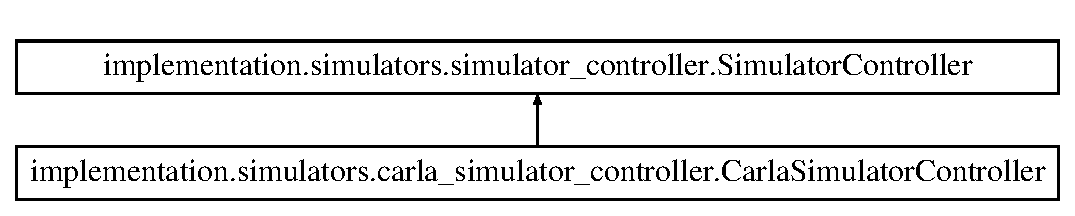
\includegraphics[height=2.000000cm]{classimplementation_1_1simulators_1_1carla__simulator__controller_1_1_carla_simulator_controller}
\end{center}
\end{figure}
\subsection*{Public Member Functions}
\begin{DoxyCompactItemize}
\item 
def \hyperlink{classimplementation_1_1simulators_1_1carla__simulator__controller_1_1_carla_simulator_controller_a36c29b90d6b1e73a76708a43eae68d1b}{\+\_\+\+\_\+init\+\_\+\+\_\+} (self)
\item 
def \hyperlink{classimplementation_1_1simulators_1_1carla__simulator__controller_1_1_carla_simulator_controller_a882ed4e896eef439a7862918b7ce0554}{connect\+\_\+simulator} (self)
\item 
def \hyperlink{classimplementation_1_1simulators_1_1carla__simulator__controller_1_1_carla_simulator_controller_abcfd1135fe7f8766890e5d20026791ef}{setup\+\_\+simulator} (self)
\item 
def \hyperlink{classimplementation_1_1simulators_1_1carla__simulator__controller_1_1_carla_simulator_controller_a263bf046ef60543b169d0d57a37e19dc}{run\+\_\+simulator\+\_\+game\+\_\+loop\+\_\+step} (self)
\item 
def \hyperlink{classimplementation_1_1simulators_1_1carla__simulator__controller_1_1_carla_simulator_controller_acd9f676fe9ce1919082465f130fadca5}{get\+\_\+sinadra\+\_\+data} (self)
\item 
def \hyperlink{classimplementation_1_1simulators_1_1carla__simulator__controller_1_1_carla_simulator_controller_a1fb507d72c2d010afbd4c3d10233668f}{get\+\_\+map} (self)
\item 
def \hyperlink{classimplementation_1_1simulators_1_1carla__simulator__controller_1_1_carla_simulator_controller_a34d719c9138b275d2bb9bd95dc5b0b34}{get\+\_\+scenario\+\_\+image} (self)
\item 
def \hyperlink{classimplementation_1_1simulators_1_1carla__simulator__controller_1_1_carla_simulator_controller_ade6f01523776f3e73bd33ccde1ac35e5}{get\+\_\+subject\+\_\+vehicle\+\_\+image} (self)
\item 
def \hyperlink{classimplementation_1_1simulators_1_1carla__simulator__controller_1_1_carla_simulator_controller_abb9bd3085d08a6b2ad2d7e72f2cd2435}{draw\+\_\+line}
\end{DoxyCompactItemize}


\subsection{Constructor \& Destructor Documentation}
\mbox{\Hypertarget{classimplementation_1_1simulators_1_1carla__simulator__controller_1_1_carla_simulator_controller_a36c29b90d6b1e73a76708a43eae68d1b}\label{classimplementation_1_1simulators_1_1carla__simulator__controller_1_1_carla_simulator_controller_a36c29b90d6b1e73a76708a43eae68d1b}} 
\index{implementation\+::simulators\+::carla\+\_\+simulator\+\_\+controller\+::\+Carla\+Simulator\+Controller@{implementation\+::simulators\+::carla\+\_\+simulator\+\_\+controller\+::\+Carla\+Simulator\+Controller}!\+\_\+\+\_\+init\+\_\+\+\_\+@{\+\_\+\+\_\+init\+\_\+\+\_\+}}
\index{\+\_\+\+\_\+init\+\_\+\+\_\+@{\+\_\+\+\_\+init\+\_\+\+\_\+}!implementation\+::simulators\+::carla\+\_\+simulator\+\_\+controller\+::\+Carla\+Simulator\+Controller@{implementation\+::simulators\+::carla\+\_\+simulator\+\_\+controller\+::\+Carla\+Simulator\+Controller}}
\subsubsection{\texorpdfstring{\+\_\+\+\_\+init\+\_\+\+\_\+()}{\_\_init\_\_()}}
{\footnotesize\ttfamily def implementation.\+simulators.\+carla\+\_\+simulator\+\_\+controller.\+Carla\+Simulator\+Controller.\+\_\+\+\_\+init\+\_\+\+\_\+ (\begin{DoxyParamCaption}\item[{}]{self,  }\item[{}]{None }\end{DoxyParamCaption})}



\subsection{Member Function Documentation}
\mbox{\Hypertarget{classimplementation_1_1simulators_1_1carla__simulator__controller_1_1_carla_simulator_controller_a882ed4e896eef439a7862918b7ce0554}\label{classimplementation_1_1simulators_1_1carla__simulator__controller_1_1_carla_simulator_controller_a882ed4e896eef439a7862918b7ce0554}} 
\index{implementation\+::simulators\+::carla\+\_\+simulator\+\_\+controller\+::\+Carla\+Simulator\+Controller@{implementation\+::simulators\+::carla\+\_\+simulator\+\_\+controller\+::\+Carla\+Simulator\+Controller}!connect\+\_\+simulator@{connect\+\_\+simulator}}
\index{connect\+\_\+simulator@{connect\+\_\+simulator}!implementation\+::simulators\+::carla\+\_\+simulator\+\_\+controller\+::\+Carla\+Simulator\+Controller@{implementation\+::simulators\+::carla\+\_\+simulator\+\_\+controller\+::\+Carla\+Simulator\+Controller}}
\subsubsection{\texorpdfstring{connect\+\_\+simulator()}{connect\_simulator()}}
{\footnotesize\ttfamily def implementation.\+simulators.\+carla\+\_\+simulator\+\_\+controller.\+Carla\+Simulator\+Controller.\+connect\+\_\+simulator (\begin{DoxyParamCaption}\item[{}]{self,  }\item[{}]{None }\end{DoxyParamCaption})}

\mbox{\Hypertarget{classimplementation_1_1simulators_1_1carla__simulator__controller_1_1_carla_simulator_controller_abb9bd3085d08a6b2ad2d7e72f2cd2435}\label{classimplementation_1_1simulators_1_1carla__simulator__controller_1_1_carla_simulator_controller_abb9bd3085d08a6b2ad2d7e72f2cd2435}} 
\index{implementation\+::simulators\+::carla\+\_\+simulator\+\_\+controller\+::\+Carla\+Simulator\+Controller@{implementation\+::simulators\+::carla\+\_\+simulator\+\_\+controller\+::\+Carla\+Simulator\+Controller}!draw\+\_\+line@{draw\+\_\+line}}
\index{draw\+\_\+line@{draw\+\_\+line}!implementation\+::simulators\+::carla\+\_\+simulator\+\_\+controller\+::\+Carla\+Simulator\+Controller@{implementation\+::simulators\+::carla\+\_\+simulator\+\_\+controller\+::\+Carla\+Simulator\+Controller}}
\subsubsection{\texorpdfstring{draw\+\_\+line()}{draw\_line()}}
{\footnotesize\ttfamily def implementation.\+simulators.\+carla\+\_\+simulator\+\_\+controller.\+Carla\+Simulator\+Controller.\+draw\+\_\+line (\begin{DoxyParamCaption}\item[{}]{self,  }\item[{}]{start }\end{DoxyParamCaption})}

\mbox{\Hypertarget{classimplementation_1_1simulators_1_1carla__simulator__controller_1_1_carla_simulator_controller_a1fb507d72c2d010afbd4c3d10233668f}\label{classimplementation_1_1simulators_1_1carla__simulator__controller_1_1_carla_simulator_controller_a1fb507d72c2d010afbd4c3d10233668f}} 
\index{implementation\+::simulators\+::carla\+\_\+simulator\+\_\+controller\+::\+Carla\+Simulator\+Controller@{implementation\+::simulators\+::carla\+\_\+simulator\+\_\+controller\+::\+Carla\+Simulator\+Controller}!get\+\_\+map@{get\+\_\+map}}
\index{get\+\_\+map@{get\+\_\+map}!implementation\+::simulators\+::carla\+\_\+simulator\+\_\+controller\+::\+Carla\+Simulator\+Controller@{implementation\+::simulators\+::carla\+\_\+simulator\+\_\+controller\+::\+Carla\+Simulator\+Controller}}
\subsubsection{\texorpdfstring{get\+\_\+map()}{get\_map()}}
{\footnotesize\ttfamily def implementation.\+simulators.\+carla\+\_\+simulator\+\_\+controller.\+Carla\+Simulator\+Controller.\+get\+\_\+map (\begin{DoxyParamCaption}\item[{}]{self,  }\item[{}]{Map }\end{DoxyParamCaption})}

\mbox{\Hypertarget{classimplementation_1_1simulators_1_1carla__simulator__controller_1_1_carla_simulator_controller_a34d719c9138b275d2bb9bd95dc5b0b34}\label{classimplementation_1_1simulators_1_1carla__simulator__controller_1_1_carla_simulator_controller_a34d719c9138b275d2bb9bd95dc5b0b34}} 
\index{implementation\+::simulators\+::carla\+\_\+simulator\+\_\+controller\+::\+Carla\+Simulator\+Controller@{implementation\+::simulators\+::carla\+\_\+simulator\+\_\+controller\+::\+Carla\+Simulator\+Controller}!get\+\_\+scenario\+\_\+image@{get\+\_\+scenario\+\_\+image}}
\index{get\+\_\+scenario\+\_\+image@{get\+\_\+scenario\+\_\+image}!implementation\+::simulators\+::carla\+\_\+simulator\+\_\+controller\+::\+Carla\+Simulator\+Controller@{implementation\+::simulators\+::carla\+\_\+simulator\+\_\+controller\+::\+Carla\+Simulator\+Controller}}
\subsubsection{\texorpdfstring{get\+\_\+scenario\+\_\+image()}{get\_scenario\_image()}}
{\footnotesize\ttfamily def implementation.\+simulators.\+carla\+\_\+simulator\+\_\+controller.\+Carla\+Simulator\+Controller.\+get\+\_\+scenario\+\_\+image (\begin{DoxyParamCaption}\item[{}]{self,  }\item[{}]{Optional,  }\item[{}]{np,  }\item[{}]{ndarray }\end{DoxyParamCaption})}

\mbox{\Hypertarget{classimplementation_1_1simulators_1_1carla__simulator__controller_1_1_carla_simulator_controller_acd9f676fe9ce1919082465f130fadca5}\label{classimplementation_1_1simulators_1_1carla__simulator__controller_1_1_carla_simulator_controller_acd9f676fe9ce1919082465f130fadca5}} 
\index{implementation\+::simulators\+::carla\+\_\+simulator\+\_\+controller\+::\+Carla\+Simulator\+Controller@{implementation\+::simulators\+::carla\+\_\+simulator\+\_\+controller\+::\+Carla\+Simulator\+Controller}!get\+\_\+sinadra\+\_\+data@{get\+\_\+sinadra\+\_\+data}}
\index{get\+\_\+sinadra\+\_\+data@{get\+\_\+sinadra\+\_\+data}!implementation\+::simulators\+::carla\+\_\+simulator\+\_\+controller\+::\+Carla\+Simulator\+Controller@{implementation\+::simulators\+::carla\+\_\+simulator\+\_\+controller\+::\+Carla\+Simulator\+Controller}}
\subsubsection{\texorpdfstring{get\+\_\+sinadra\+\_\+data()}{get\_sinadra\_data()}}
{\footnotesize\ttfamily def implementation.\+simulators.\+carla\+\_\+simulator\+\_\+controller.\+Carla\+Simulator\+Controller.\+get\+\_\+sinadra\+\_\+data (\begin{DoxyParamCaption}\item[{}]{self,  }\item[{}]{Optional,  }\item[{}]{Sinadra\+Data }\end{DoxyParamCaption})}

\mbox{\Hypertarget{classimplementation_1_1simulators_1_1carla__simulator__controller_1_1_carla_simulator_controller_ade6f01523776f3e73bd33ccde1ac35e5}\label{classimplementation_1_1simulators_1_1carla__simulator__controller_1_1_carla_simulator_controller_ade6f01523776f3e73bd33ccde1ac35e5}} 
\index{implementation\+::simulators\+::carla\+\_\+simulator\+\_\+controller\+::\+Carla\+Simulator\+Controller@{implementation\+::simulators\+::carla\+\_\+simulator\+\_\+controller\+::\+Carla\+Simulator\+Controller}!get\+\_\+subject\+\_\+vehicle\+\_\+image@{get\+\_\+subject\+\_\+vehicle\+\_\+image}}
\index{get\+\_\+subject\+\_\+vehicle\+\_\+image@{get\+\_\+subject\+\_\+vehicle\+\_\+image}!implementation\+::simulators\+::carla\+\_\+simulator\+\_\+controller\+::\+Carla\+Simulator\+Controller@{implementation\+::simulators\+::carla\+\_\+simulator\+\_\+controller\+::\+Carla\+Simulator\+Controller}}
\subsubsection{\texorpdfstring{get\+\_\+subject\+\_\+vehicle\+\_\+image()}{get\_subject\_vehicle\_image()}}
{\footnotesize\ttfamily def implementation.\+simulators.\+carla\+\_\+simulator\+\_\+controller.\+Carla\+Simulator\+Controller.\+get\+\_\+subject\+\_\+vehicle\+\_\+image (\begin{DoxyParamCaption}\item[{}]{self,  }\item[{}]{Optional,  }\item[{}]{np,  }\item[{}]{ndarray }\end{DoxyParamCaption})}

\mbox{\Hypertarget{classimplementation_1_1simulators_1_1carla__simulator__controller_1_1_carla_simulator_controller_a263bf046ef60543b169d0d57a37e19dc}\label{classimplementation_1_1simulators_1_1carla__simulator__controller_1_1_carla_simulator_controller_a263bf046ef60543b169d0d57a37e19dc}} 
\index{implementation\+::simulators\+::carla\+\_\+simulator\+\_\+controller\+::\+Carla\+Simulator\+Controller@{implementation\+::simulators\+::carla\+\_\+simulator\+\_\+controller\+::\+Carla\+Simulator\+Controller}!run\+\_\+simulator\+\_\+game\+\_\+loop\+\_\+step@{run\+\_\+simulator\+\_\+game\+\_\+loop\+\_\+step}}
\index{run\+\_\+simulator\+\_\+game\+\_\+loop\+\_\+step@{run\+\_\+simulator\+\_\+game\+\_\+loop\+\_\+step}!implementation\+::simulators\+::carla\+\_\+simulator\+\_\+controller\+::\+Carla\+Simulator\+Controller@{implementation\+::simulators\+::carla\+\_\+simulator\+\_\+controller\+::\+Carla\+Simulator\+Controller}}
\subsubsection{\texorpdfstring{run\+\_\+simulator\+\_\+game\+\_\+loop\+\_\+step()}{run\_simulator\_game\_loop\_step()}}
{\footnotesize\ttfamily def implementation.\+simulators.\+carla\+\_\+simulator\+\_\+controller.\+Carla\+Simulator\+Controller.\+run\+\_\+simulator\+\_\+game\+\_\+loop\+\_\+step (\begin{DoxyParamCaption}\item[{}]{self,  }\item[{}]{None }\end{DoxyParamCaption})}

\mbox{\Hypertarget{classimplementation_1_1simulators_1_1carla__simulator__controller_1_1_carla_simulator_controller_abcfd1135fe7f8766890e5d20026791ef}\label{classimplementation_1_1simulators_1_1carla__simulator__controller_1_1_carla_simulator_controller_abcfd1135fe7f8766890e5d20026791ef}} 
\index{implementation\+::simulators\+::carla\+\_\+simulator\+\_\+controller\+::\+Carla\+Simulator\+Controller@{implementation\+::simulators\+::carla\+\_\+simulator\+\_\+controller\+::\+Carla\+Simulator\+Controller}!setup\+\_\+simulator@{setup\+\_\+simulator}}
\index{setup\+\_\+simulator@{setup\+\_\+simulator}!implementation\+::simulators\+::carla\+\_\+simulator\+\_\+controller\+::\+Carla\+Simulator\+Controller@{implementation\+::simulators\+::carla\+\_\+simulator\+\_\+controller\+::\+Carla\+Simulator\+Controller}}
\subsubsection{\texorpdfstring{setup\+\_\+simulator()}{setup\_simulator()}}
{\footnotesize\ttfamily def implementation.\+simulators.\+carla\+\_\+simulator\+\_\+controller.\+Carla\+Simulator\+Controller.\+setup\+\_\+simulator (\begin{DoxyParamCaption}\item[{}]{self,  }\item[{}]{None }\end{DoxyParamCaption})}



The documentation for this class was generated from the following file\+:\begin{DoxyCompactItemize}
\item 
implementation/simulators/\hyperlink{carla__simulator__controller_8py}{carla\+\_\+simulator\+\_\+controller.\+py}\end{DoxyCompactItemize}

\hypertarget{classimplementation_1_1simulators_1_1carla__sinadra__data__handler_1_1_carla_sinadra_data_handler}{}\section{implementation.\+simulators.\+carla\+\_\+sinadra\+\_\+data\+\_\+handler.\+Carla\+Sinadra\+Data\+Handler Class Reference}
\label{classimplementation_1_1simulators_1_1carla__sinadra__data__handler_1_1_carla_sinadra_data_handler}\index{implementation.\+simulators.\+carla\+\_\+sinadra\+\_\+data\+\_\+handler.\+Carla\+Sinadra\+Data\+Handler@{implementation.\+simulators.\+carla\+\_\+sinadra\+\_\+data\+\_\+handler.\+Carla\+Sinadra\+Data\+Handler}}
Inheritance diagram for implementation.\+simulators.\+carla\+\_\+sinadra\+\_\+data\+\_\+handler.\+Carla\+Sinadra\+Data\+Handler\+:\begin{figure}[H]
\begin{center}
\leavevmode
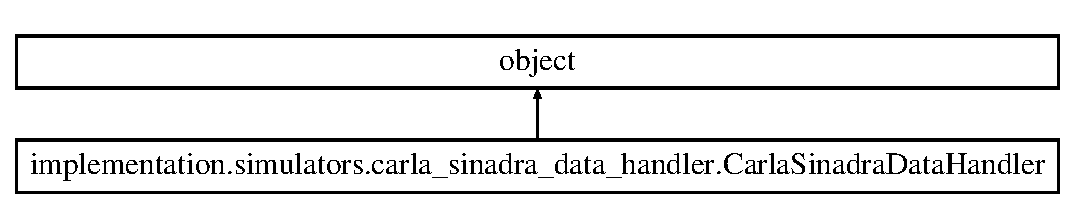
\includegraphics[height=2.000000cm]{classimplementation_1_1simulators_1_1carla__sinadra__data__handler_1_1_carla_sinadra_data_handler}
\end{center}
\end{figure}
\subsection*{Public Member Functions}
\begin{DoxyCompactItemize}
\item 
def \hyperlink{classimplementation_1_1simulators_1_1carla__sinadra__data__handler_1_1_carla_sinadra_data_handler_a72fd74b953ea679883a720ba612136ab}{\+\_\+\+\_\+init\+\_\+\+\_\+} (self)
\item 
def \hyperlink{classimplementation_1_1simulators_1_1carla__sinadra__data__handler_1_1_carla_sinadra_data_handler_aa506562e73fc5609b024ea59e253943a}{populate\+\_\+data\+\_\+model}
\end{DoxyCompactItemize}


\subsection{Constructor \& Destructor Documentation}
\mbox{\Hypertarget{classimplementation_1_1simulators_1_1carla__sinadra__data__handler_1_1_carla_sinadra_data_handler_a72fd74b953ea679883a720ba612136ab}\label{classimplementation_1_1simulators_1_1carla__sinadra__data__handler_1_1_carla_sinadra_data_handler_a72fd74b953ea679883a720ba612136ab}} 
\index{implementation\+::simulators\+::carla\+\_\+sinadra\+\_\+data\+\_\+handler\+::\+Carla\+Sinadra\+Data\+Handler@{implementation\+::simulators\+::carla\+\_\+sinadra\+\_\+data\+\_\+handler\+::\+Carla\+Sinadra\+Data\+Handler}!\+\_\+\+\_\+init\+\_\+\+\_\+@{\+\_\+\+\_\+init\+\_\+\+\_\+}}
\index{\+\_\+\+\_\+init\+\_\+\+\_\+@{\+\_\+\+\_\+init\+\_\+\+\_\+}!implementation\+::simulators\+::carla\+\_\+sinadra\+\_\+data\+\_\+handler\+::\+Carla\+Sinadra\+Data\+Handler@{implementation\+::simulators\+::carla\+\_\+sinadra\+\_\+data\+\_\+handler\+::\+Carla\+Sinadra\+Data\+Handler}}
\subsubsection{\texorpdfstring{\+\_\+\+\_\+init\+\_\+\+\_\+()}{\_\_init\_\_()}}
{\footnotesize\ttfamily def implementation.\+simulators.\+carla\+\_\+sinadra\+\_\+data\+\_\+handler.\+Carla\+Sinadra\+Data\+Handler.\+\_\+\+\_\+init\+\_\+\+\_\+ (\begin{DoxyParamCaption}\item[{}]{self }\end{DoxyParamCaption})}



\subsection{Member Function Documentation}
\mbox{\Hypertarget{classimplementation_1_1simulators_1_1carla__sinadra__data__handler_1_1_carla_sinadra_data_handler_aa506562e73fc5609b024ea59e253943a}\label{classimplementation_1_1simulators_1_1carla__sinadra__data__handler_1_1_carla_sinadra_data_handler_aa506562e73fc5609b024ea59e253943a}} 
\index{implementation\+::simulators\+::carla\+\_\+sinadra\+\_\+data\+\_\+handler\+::\+Carla\+Sinadra\+Data\+Handler@{implementation\+::simulators\+::carla\+\_\+sinadra\+\_\+data\+\_\+handler\+::\+Carla\+Sinadra\+Data\+Handler}!populate\+\_\+data\+\_\+model@{populate\+\_\+data\+\_\+model}}
\index{populate\+\_\+data\+\_\+model@{populate\+\_\+data\+\_\+model}!implementation\+::simulators\+::carla\+\_\+sinadra\+\_\+data\+\_\+handler\+::\+Carla\+Sinadra\+Data\+Handler@{implementation\+::simulators\+::carla\+\_\+sinadra\+\_\+data\+\_\+handler\+::\+Carla\+Sinadra\+Data\+Handler}}
\subsubsection{\texorpdfstring{populate\+\_\+data\+\_\+model()}{populate\_data\_model()}}
{\footnotesize\ttfamily def implementation.\+simulators.\+carla\+\_\+sinadra\+\_\+data\+\_\+handler.\+Carla\+Sinadra\+Data\+Handler.\+populate\+\_\+data\+\_\+model (\begin{DoxyParamCaption}\item[{}]{self,  }\item[{}]{hero\+\_\+vehicle }\end{DoxyParamCaption})}



The documentation for this class was generated from the following file\+:\begin{DoxyCompactItemize}
\item 
implementation/simulators/\hyperlink{carla__sinadra__data__handler_8py}{carla\+\_\+sinadra\+\_\+data\+\_\+handler.\+py}\end{DoxyCompactItemize}

\hypertarget{classimplementation_1_1data__model_1_1environment_1_1_cloud_state}{}\section{implementation.\+data\+\_\+model.\+environment.\+Cloud\+State Class Reference}
\label{classimplementation_1_1data__model_1_1environment_1_1_cloud_state}\index{implementation.\+data\+\_\+model.\+environment.\+Cloud\+State@{implementation.\+data\+\_\+model.\+environment.\+Cloud\+State}}
Inheritance diagram for implementation.\+data\+\_\+model.\+environment.\+Cloud\+State\+:\begin{figure}[H]
\begin{center}
\leavevmode
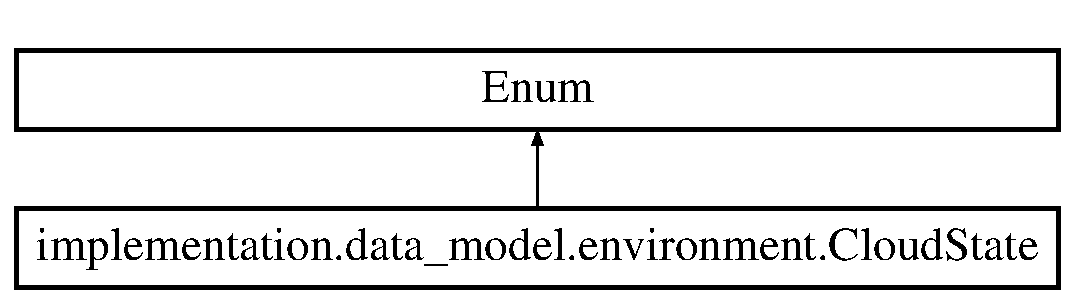
\includegraphics[height=2.000000cm]{classimplementation_1_1data__model_1_1environment_1_1_cloud_state}
\end{center}
\end{figure}
\subsection*{Static Public Attributes}
\begin{DoxyCompactItemize}
\item 
int \hyperlink{classimplementation_1_1data__model_1_1environment_1_1_cloud_state_a1679ec829e242670aca715b8cd3b056e}{F\+R\+EE} = 1
\item 
int \hyperlink{classimplementation_1_1data__model_1_1environment_1_1_cloud_state_a44ce6c694691a43221b7b3981a250807}{C\+L\+O\+U\+DY} = 2
\item 
int \hyperlink{classimplementation_1_1data__model_1_1environment_1_1_cloud_state_a450787a5846864ae481bb94b196cc622}{O\+V\+E\+R\+C\+A\+ST} = 3
\item 
int \hyperlink{classimplementation_1_1data__model_1_1environment_1_1_cloud_state_a418bf3040ff7a0429a426d86942dcea3}{R\+A\+I\+NY} = 4
\item 
int \hyperlink{classimplementation_1_1data__model_1_1environment_1_1_cloud_state_a4ca8feddafca201b25c2616622a75187}{S\+K\+Y\+\_\+\+O\+FF} = 5
\end{DoxyCompactItemize}


\subsection{Member Data Documentation}
\mbox{\Hypertarget{classimplementation_1_1data__model_1_1environment_1_1_cloud_state_a44ce6c694691a43221b7b3981a250807}\label{classimplementation_1_1data__model_1_1environment_1_1_cloud_state_a44ce6c694691a43221b7b3981a250807}} 
\index{implementation\+::data\+\_\+model\+::environment\+::\+Cloud\+State@{implementation\+::data\+\_\+model\+::environment\+::\+Cloud\+State}!C\+L\+O\+U\+DY@{C\+L\+O\+U\+DY}}
\index{C\+L\+O\+U\+DY@{C\+L\+O\+U\+DY}!implementation\+::data\+\_\+model\+::environment\+::\+Cloud\+State@{implementation\+::data\+\_\+model\+::environment\+::\+Cloud\+State}}
\subsubsection{\texorpdfstring{C\+L\+O\+U\+DY}{CLOUDY}}
{\footnotesize\ttfamily int implementation.\+data\+\_\+model.\+environment.\+Cloud\+State.\+C\+L\+O\+U\+DY = 2\hspace{0.3cm}{\ttfamily [static]}}

\mbox{\Hypertarget{classimplementation_1_1data__model_1_1environment_1_1_cloud_state_a1679ec829e242670aca715b8cd3b056e}\label{classimplementation_1_1data__model_1_1environment_1_1_cloud_state_a1679ec829e242670aca715b8cd3b056e}} 
\index{implementation\+::data\+\_\+model\+::environment\+::\+Cloud\+State@{implementation\+::data\+\_\+model\+::environment\+::\+Cloud\+State}!F\+R\+EE@{F\+R\+EE}}
\index{F\+R\+EE@{F\+R\+EE}!implementation\+::data\+\_\+model\+::environment\+::\+Cloud\+State@{implementation\+::data\+\_\+model\+::environment\+::\+Cloud\+State}}
\subsubsection{\texorpdfstring{F\+R\+EE}{FREE}}
{\footnotesize\ttfamily int implementation.\+data\+\_\+model.\+environment.\+Cloud\+State.\+F\+R\+EE = 1\hspace{0.3cm}{\ttfamily [static]}}

\mbox{\Hypertarget{classimplementation_1_1data__model_1_1environment_1_1_cloud_state_a450787a5846864ae481bb94b196cc622}\label{classimplementation_1_1data__model_1_1environment_1_1_cloud_state_a450787a5846864ae481bb94b196cc622}} 
\index{implementation\+::data\+\_\+model\+::environment\+::\+Cloud\+State@{implementation\+::data\+\_\+model\+::environment\+::\+Cloud\+State}!O\+V\+E\+R\+C\+A\+ST@{O\+V\+E\+R\+C\+A\+ST}}
\index{O\+V\+E\+R\+C\+A\+ST@{O\+V\+E\+R\+C\+A\+ST}!implementation\+::data\+\_\+model\+::environment\+::\+Cloud\+State@{implementation\+::data\+\_\+model\+::environment\+::\+Cloud\+State}}
\subsubsection{\texorpdfstring{O\+V\+E\+R\+C\+A\+ST}{OVERCAST}}
{\footnotesize\ttfamily int implementation.\+data\+\_\+model.\+environment.\+Cloud\+State.\+O\+V\+E\+R\+C\+A\+ST = 3\hspace{0.3cm}{\ttfamily [static]}}

\mbox{\Hypertarget{classimplementation_1_1data__model_1_1environment_1_1_cloud_state_a418bf3040ff7a0429a426d86942dcea3}\label{classimplementation_1_1data__model_1_1environment_1_1_cloud_state_a418bf3040ff7a0429a426d86942dcea3}} 
\index{implementation\+::data\+\_\+model\+::environment\+::\+Cloud\+State@{implementation\+::data\+\_\+model\+::environment\+::\+Cloud\+State}!R\+A\+I\+NY@{R\+A\+I\+NY}}
\index{R\+A\+I\+NY@{R\+A\+I\+NY}!implementation\+::data\+\_\+model\+::environment\+::\+Cloud\+State@{implementation\+::data\+\_\+model\+::environment\+::\+Cloud\+State}}
\subsubsection{\texorpdfstring{R\+A\+I\+NY}{RAINY}}
{\footnotesize\ttfamily int implementation.\+data\+\_\+model.\+environment.\+Cloud\+State.\+R\+A\+I\+NY = 4\hspace{0.3cm}{\ttfamily [static]}}

\mbox{\Hypertarget{classimplementation_1_1data__model_1_1environment_1_1_cloud_state_a4ca8feddafca201b25c2616622a75187}\label{classimplementation_1_1data__model_1_1environment_1_1_cloud_state_a4ca8feddafca201b25c2616622a75187}} 
\index{implementation\+::data\+\_\+model\+::environment\+::\+Cloud\+State@{implementation\+::data\+\_\+model\+::environment\+::\+Cloud\+State}!S\+K\+Y\+\_\+\+O\+FF@{S\+K\+Y\+\_\+\+O\+FF}}
\index{S\+K\+Y\+\_\+\+O\+FF@{S\+K\+Y\+\_\+\+O\+FF}!implementation\+::data\+\_\+model\+::environment\+::\+Cloud\+State@{implementation\+::data\+\_\+model\+::environment\+::\+Cloud\+State}}
\subsubsection{\texorpdfstring{S\+K\+Y\+\_\+\+O\+FF}{SKY\_OFF}}
{\footnotesize\ttfamily int implementation.\+data\+\_\+model.\+environment.\+Cloud\+State.\+S\+K\+Y\+\_\+\+O\+FF = 5\hspace{0.3cm}{\ttfamily [static]}}



The documentation for this class was generated from the following file\+:\begin{DoxyCompactItemize}
\item 
implementation/data\+\_\+model/\hyperlink{environment_8py}{environment.\+py}\end{DoxyCompactItemize}

\hypertarget{classimplementation_1_1manual__control_1_1_collision_sensor}{}\doxysection{implementation.\+manual\+\_\+control.\+Collision\+Sensor Class Reference}
\label{classimplementation_1_1manual__control_1_1_collision_sensor}\index{implementation.manual\_control.CollisionSensor@{implementation.manual\_control.CollisionSensor}}
Inheritance diagram for implementation.\+manual\+\_\+control.\+Collision\+Sensor\+:\begin{figure}[H]
\begin{center}
\leavevmode
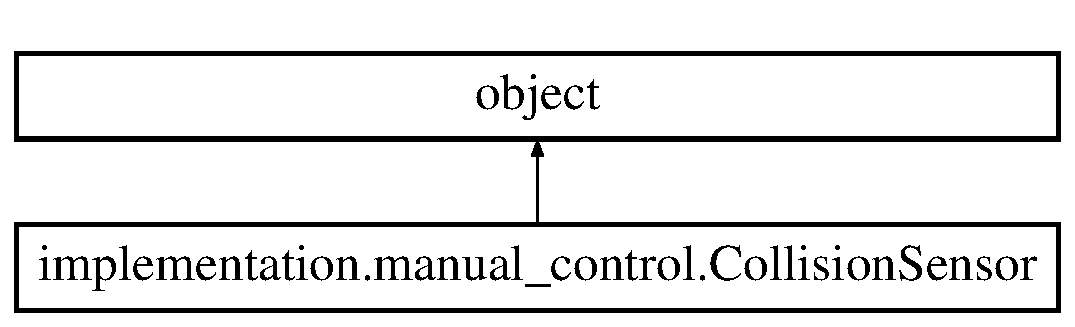
\includegraphics[height=2.000000cm]{classimplementation_1_1manual__control_1_1_collision_sensor}
\end{center}
\end{figure}
\doxysubsection*{Public Member Functions}
\begin{DoxyCompactItemize}
\item 
def \mbox{\hyperlink{classimplementation_1_1manual__control_1_1_collision_sensor_aa60cd8ac42d412ca5d780332e1785916}{\+\_\+\+\_\+init\+\_\+\+\_\+}} (self, parent\+\_\+actor, \mbox{\hyperlink{classimplementation_1_1manual__control_1_1_collision_sensor_a207937a78ede8085241d480d419f157f}{hud}})
\item 
def \mbox{\hyperlink{classimplementation_1_1manual__control_1_1_collision_sensor_ad71f3095c743ed6a44e4424ae865276f}{get\+\_\+collision\+\_\+history}} (self)
\end{DoxyCompactItemize}
\doxysubsection*{Public Attributes}
\begin{DoxyCompactItemize}
\item 
\mbox{\hyperlink{classimplementation_1_1manual__control_1_1_collision_sensor_a3c7f37286c361206b0b5c6d89878cd90}{sensor}}
\item 
\mbox{\hyperlink{classimplementation_1_1manual__control_1_1_collision_sensor_a5ba30843b06e1f424b620067aea9dafe}{history}}
\item 
\mbox{\hyperlink{classimplementation_1_1manual__control_1_1_collision_sensor_a207937a78ede8085241d480d419f157f}{hud}}
\end{DoxyCompactItemize}


\doxysubsection{Constructor \& Destructor Documentation}
\mbox{\Hypertarget{classimplementation_1_1manual__control_1_1_collision_sensor_aa60cd8ac42d412ca5d780332e1785916}\label{classimplementation_1_1manual__control_1_1_collision_sensor_aa60cd8ac42d412ca5d780332e1785916}} 
\index{implementation.manual\_control.CollisionSensor@{implementation.manual\_control.CollisionSensor}!\_\_init\_\_@{\_\_init\_\_}}
\index{\_\_init\_\_@{\_\_init\_\_}!implementation.manual\_control.CollisionSensor@{implementation.manual\_control.CollisionSensor}}
\doxysubsubsection{\texorpdfstring{\_\_init\_\_()}{\_\_init\_\_()}}
{\footnotesize\ttfamily def implementation.\+manual\+\_\+control.\+Collision\+Sensor.\+\_\+\+\_\+init\+\_\+\+\_\+ (\begin{DoxyParamCaption}\item[{}]{self,  }\item[{}]{parent\+\_\+actor,  }\item[{}]{hud }\end{DoxyParamCaption})}



\doxysubsection{Member Function Documentation}
\mbox{\Hypertarget{classimplementation_1_1manual__control_1_1_collision_sensor_ad71f3095c743ed6a44e4424ae865276f}\label{classimplementation_1_1manual__control_1_1_collision_sensor_ad71f3095c743ed6a44e4424ae865276f}} 
\index{implementation.manual\_control.CollisionSensor@{implementation.manual\_control.CollisionSensor}!get\_collision\_history@{get\_collision\_history}}
\index{get\_collision\_history@{get\_collision\_history}!implementation.manual\_control.CollisionSensor@{implementation.manual\_control.CollisionSensor}}
\doxysubsubsection{\texorpdfstring{get\_collision\_history()}{get\_collision\_history()}}
{\footnotesize\ttfamily def implementation.\+manual\+\_\+control.\+Collision\+Sensor.\+get\+\_\+collision\+\_\+history (\begin{DoxyParamCaption}\item[{}]{self }\end{DoxyParamCaption})}



\doxysubsection{Member Data Documentation}
\mbox{\Hypertarget{classimplementation_1_1manual__control_1_1_collision_sensor_a5ba30843b06e1f424b620067aea9dafe}\label{classimplementation_1_1manual__control_1_1_collision_sensor_a5ba30843b06e1f424b620067aea9dafe}} 
\index{implementation.manual\_control.CollisionSensor@{implementation.manual\_control.CollisionSensor}!history@{history}}
\index{history@{history}!implementation.manual\_control.CollisionSensor@{implementation.manual\_control.CollisionSensor}}
\doxysubsubsection{\texorpdfstring{history}{history}}
{\footnotesize\ttfamily implementation.\+manual\+\_\+control.\+Collision\+Sensor.\+history}

\mbox{\Hypertarget{classimplementation_1_1manual__control_1_1_collision_sensor_a207937a78ede8085241d480d419f157f}\label{classimplementation_1_1manual__control_1_1_collision_sensor_a207937a78ede8085241d480d419f157f}} 
\index{implementation.manual\_control.CollisionSensor@{implementation.manual\_control.CollisionSensor}!hud@{hud}}
\index{hud@{hud}!implementation.manual\_control.CollisionSensor@{implementation.manual\_control.CollisionSensor}}
\doxysubsubsection{\texorpdfstring{hud}{hud}}
{\footnotesize\ttfamily implementation.\+manual\+\_\+control.\+Collision\+Sensor.\+hud}

\mbox{\Hypertarget{classimplementation_1_1manual__control_1_1_collision_sensor_a3c7f37286c361206b0b5c6d89878cd90}\label{classimplementation_1_1manual__control_1_1_collision_sensor_a3c7f37286c361206b0b5c6d89878cd90}} 
\index{implementation.manual\_control.CollisionSensor@{implementation.manual\_control.CollisionSensor}!sensor@{sensor}}
\index{sensor@{sensor}!implementation.manual\_control.CollisionSensor@{implementation.manual\_control.CollisionSensor}}
\doxysubsubsection{\texorpdfstring{sensor}{sensor}}
{\footnotesize\ttfamily implementation.\+manual\+\_\+control.\+Collision\+Sensor.\+sensor}



The documentation for this class was generated from the following file\+:\begin{DoxyCompactItemize}
\item 
implementation/\mbox{\hyperlink{manual__control_8py}{manual\+\_\+control.\+py}}\end{DoxyCompactItemize}

\hypertarget{classimplementation_1_1bayesian__network_1_1inference_1_1sinadra__risk__sensor__data_1_1_cut_in_from_left}{}\section{implementation.\+bayesian\+\_\+network.\+inference.\+sinadra\+\_\+risk\+\_\+sensor\+\_\+data.\+Cut\+In\+From\+Left Class Reference}
\label{classimplementation_1_1bayesian__network_1_1inference_1_1sinadra__risk__sensor__data_1_1_cut_in_from_left}\index{implementation.\+bayesian\+\_\+network.\+inference.\+sinadra\+\_\+risk\+\_\+sensor\+\_\+data.\+Cut\+In\+From\+Left@{implementation.\+bayesian\+\_\+network.\+inference.\+sinadra\+\_\+risk\+\_\+sensor\+\_\+data.\+Cut\+In\+From\+Left}}
Inheritance diagram for implementation.\+bayesian\+\_\+network.\+inference.\+sinadra\+\_\+risk\+\_\+sensor\+\_\+data.\+Cut\+In\+From\+Left\+:\begin{figure}[H]
\begin{center}
\leavevmode
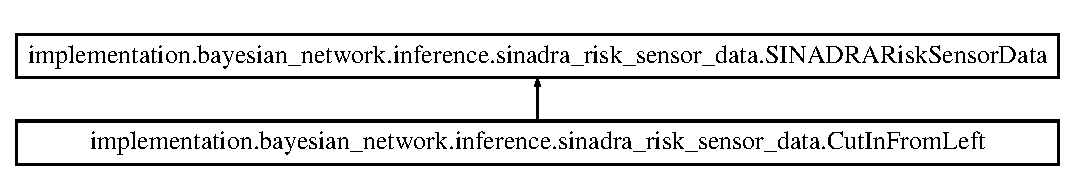
\includegraphics[height=1.989343cm]{classimplementation_1_1bayesian__network_1_1inference_1_1sinadra__risk__sensor__data_1_1_cut_in_from_left}
\end{center}
\end{figure}
\subsection*{Public Member Functions}
\begin{DoxyCompactItemize}
\item 
def \hyperlink{classimplementation_1_1bayesian__network_1_1inference_1_1sinadra__risk__sensor__data_1_1_cut_in_from_left_a6036f843dffbf16aba9cf950d6ccefa1}{\+\_\+\+\_\+init\+\_\+\+\_\+} (self)
\item 
def \hyperlink{classimplementation_1_1bayesian__network_1_1inference_1_1sinadra__risk__sensor__data_1_1_cut_in_from_left_a40bc2bd36793756ca55c297073ea1bbe}{collect\+\_\+data\+\_\+from\+\_\+carla}
\end{DoxyCompactItemize}
\subsection*{Public Attributes}
\begin{DoxyCompactItemize}
\item 
\hyperlink{classimplementation_1_1bayesian__network_1_1inference_1_1sinadra__risk__sensor__data_1_1_cut_in_from_left_a8ae675bc5a950e901d5fee8ae9bc8ab7}{vehicle\+\_\+speed}
\item 
\hyperlink{classimplementation_1_1bayesian__network_1_1inference_1_1sinadra__risk__sensor__data_1_1_cut_in_from_left_ad4afa56493c13fdb1bd27360ac65caf5}{vehicle\+\_\+length}
\item 
\hyperlink{classimplementation_1_1bayesian__network_1_1inference_1_1sinadra__risk__sensor__data_1_1_cut_in_from_left_a27857842a4c1059a380b32e68b7b916f}{is\+\_\+raining\+\_\+heavy}
\item 
\hyperlink{classimplementation_1_1bayesian__network_1_1inference_1_1sinadra__risk__sensor__data_1_1_cut_in_from_left_a6306d37e719f1ad02344d9ea22329bb9}{is\+\_\+indicating\+\_\+lane\+\_\+change}
\item 
\hyperlink{classimplementation_1_1bayesian__network_1_1inference_1_1sinadra__risk__sensor__data_1_1_cut_in_from_left_a703cf71b7ba578ed8a690e236830dad0}{distance\+\_\+to\+\_\+lane\+\_\+end}
\item 
\hyperlink{classimplementation_1_1bayesian__network_1_1inference_1_1sinadra__risk__sensor__data_1_1_cut_in_from_left_a36e8e0dcd180aeee89b0f4309744becc}{right\+\_\+cut\+\_\+in\+\_\+gap\+\_\+size}
\item 
\hyperlink{classimplementation_1_1bayesian__network_1_1inference_1_1sinadra__risk__sensor__data_1_1_cut_in_from_left_aad316a4a9a7ff4baca20a9c3a114f9c9}{steering\+\_\+angle\+\_\+from\+\_\+lane\+\_\+following}
\item 
\hyperlink{classimplementation_1_1bayesian__network_1_1inference_1_1sinadra__risk__sensor__data_1_1_cut_in_from_left_a7d99667ecaa2732f6272b837ec8de7ed}{distance\+\_\+from\+\_\+right\+\_\+lane\+\_\+line}
\item 
\hyperlink{classimplementation_1_1bayesian__network_1_1inference_1_1sinadra__risk__sensor__data_1_1_cut_in_from_left_a3980dc9774b8f547d93a89e1875b1577}{distance\+\_\+from\+\_\+lane\+\_\+center}
\end{DoxyCompactItemize}


\subsection{Constructor \& Destructor Documentation}
\mbox{\Hypertarget{classimplementation_1_1bayesian__network_1_1inference_1_1sinadra__risk__sensor__data_1_1_cut_in_from_left_a6036f843dffbf16aba9cf950d6ccefa1}\label{classimplementation_1_1bayesian__network_1_1inference_1_1sinadra__risk__sensor__data_1_1_cut_in_from_left_a6036f843dffbf16aba9cf950d6ccefa1}} 
\index{implementation\+::bayesian\+\_\+network\+::inference\+::sinadra\+\_\+risk\+\_\+sensor\+\_\+data\+::\+Cut\+In\+From\+Left@{implementation\+::bayesian\+\_\+network\+::inference\+::sinadra\+\_\+risk\+\_\+sensor\+\_\+data\+::\+Cut\+In\+From\+Left}!\+\_\+\+\_\+init\+\_\+\+\_\+@{\+\_\+\+\_\+init\+\_\+\+\_\+}}
\index{\+\_\+\+\_\+init\+\_\+\+\_\+@{\+\_\+\+\_\+init\+\_\+\+\_\+}!implementation\+::bayesian\+\_\+network\+::inference\+::sinadra\+\_\+risk\+\_\+sensor\+\_\+data\+::\+Cut\+In\+From\+Left@{implementation\+::bayesian\+\_\+network\+::inference\+::sinadra\+\_\+risk\+\_\+sensor\+\_\+data\+::\+Cut\+In\+From\+Left}}
\subsubsection{\texorpdfstring{\+\_\+\+\_\+init\+\_\+\+\_\+()}{\_\_init\_\_()}}
{\footnotesize\ttfamily def implementation.\+bayesian\+\_\+network.\+inference.\+sinadra\+\_\+risk\+\_\+sensor\+\_\+data.\+Cut\+In\+From\+Left.\+\_\+\+\_\+init\+\_\+\+\_\+ (\begin{DoxyParamCaption}\item[{}]{self }\end{DoxyParamCaption})}



\subsection{Member Function Documentation}
\mbox{\Hypertarget{classimplementation_1_1bayesian__network_1_1inference_1_1sinadra__risk__sensor__data_1_1_cut_in_from_left_a40bc2bd36793756ca55c297073ea1bbe}\label{classimplementation_1_1bayesian__network_1_1inference_1_1sinadra__risk__sensor__data_1_1_cut_in_from_left_a40bc2bd36793756ca55c297073ea1bbe}} 
\index{implementation\+::bayesian\+\_\+network\+::inference\+::sinadra\+\_\+risk\+\_\+sensor\+\_\+data\+::\+Cut\+In\+From\+Left@{implementation\+::bayesian\+\_\+network\+::inference\+::sinadra\+\_\+risk\+\_\+sensor\+\_\+data\+::\+Cut\+In\+From\+Left}!collect\+\_\+data\+\_\+from\+\_\+carla@{collect\+\_\+data\+\_\+from\+\_\+carla}}
\index{collect\+\_\+data\+\_\+from\+\_\+carla@{collect\+\_\+data\+\_\+from\+\_\+carla}!implementation\+::bayesian\+\_\+network\+::inference\+::sinadra\+\_\+risk\+\_\+sensor\+\_\+data\+::\+Cut\+In\+From\+Left@{implementation\+::bayesian\+\_\+network\+::inference\+::sinadra\+\_\+risk\+\_\+sensor\+\_\+data\+::\+Cut\+In\+From\+Left}}
\subsubsection{\texorpdfstring{collect\+\_\+data\+\_\+from\+\_\+carla()}{collect\_data\_from\_carla()}}
{\footnotesize\ttfamily def implementation.\+bayesian\+\_\+network.\+inference.\+sinadra\+\_\+risk\+\_\+sensor\+\_\+data.\+Cut\+In\+From\+Left.\+collect\+\_\+data\+\_\+from\+\_\+carla (\begin{DoxyParamCaption}\item[{}]{self,  }\item[{}]{input\+\_\+feature\+\_\+data }\end{DoxyParamCaption})}



\subsection{Member Data Documentation}
\mbox{\Hypertarget{classimplementation_1_1bayesian__network_1_1inference_1_1sinadra__risk__sensor__data_1_1_cut_in_from_left_a3980dc9774b8f547d93a89e1875b1577}\label{classimplementation_1_1bayesian__network_1_1inference_1_1sinadra__risk__sensor__data_1_1_cut_in_from_left_a3980dc9774b8f547d93a89e1875b1577}} 
\index{implementation\+::bayesian\+\_\+network\+::inference\+::sinadra\+\_\+risk\+\_\+sensor\+\_\+data\+::\+Cut\+In\+From\+Left@{implementation\+::bayesian\+\_\+network\+::inference\+::sinadra\+\_\+risk\+\_\+sensor\+\_\+data\+::\+Cut\+In\+From\+Left}!distance\+\_\+from\+\_\+lane\+\_\+center@{distance\+\_\+from\+\_\+lane\+\_\+center}}
\index{distance\+\_\+from\+\_\+lane\+\_\+center@{distance\+\_\+from\+\_\+lane\+\_\+center}!implementation\+::bayesian\+\_\+network\+::inference\+::sinadra\+\_\+risk\+\_\+sensor\+\_\+data\+::\+Cut\+In\+From\+Left@{implementation\+::bayesian\+\_\+network\+::inference\+::sinadra\+\_\+risk\+\_\+sensor\+\_\+data\+::\+Cut\+In\+From\+Left}}
\subsubsection{\texorpdfstring{distance\+\_\+from\+\_\+lane\+\_\+center}{distance\_from\_lane\_center}}
{\footnotesize\ttfamily implementation.\+bayesian\+\_\+network.\+inference.\+sinadra\+\_\+risk\+\_\+sensor\+\_\+data.\+Cut\+In\+From\+Left.\+distance\+\_\+from\+\_\+lane\+\_\+center}

\mbox{\Hypertarget{classimplementation_1_1bayesian__network_1_1inference_1_1sinadra__risk__sensor__data_1_1_cut_in_from_left_a7d99667ecaa2732f6272b837ec8de7ed}\label{classimplementation_1_1bayesian__network_1_1inference_1_1sinadra__risk__sensor__data_1_1_cut_in_from_left_a7d99667ecaa2732f6272b837ec8de7ed}} 
\index{implementation\+::bayesian\+\_\+network\+::inference\+::sinadra\+\_\+risk\+\_\+sensor\+\_\+data\+::\+Cut\+In\+From\+Left@{implementation\+::bayesian\+\_\+network\+::inference\+::sinadra\+\_\+risk\+\_\+sensor\+\_\+data\+::\+Cut\+In\+From\+Left}!distance\+\_\+from\+\_\+right\+\_\+lane\+\_\+line@{distance\+\_\+from\+\_\+right\+\_\+lane\+\_\+line}}
\index{distance\+\_\+from\+\_\+right\+\_\+lane\+\_\+line@{distance\+\_\+from\+\_\+right\+\_\+lane\+\_\+line}!implementation\+::bayesian\+\_\+network\+::inference\+::sinadra\+\_\+risk\+\_\+sensor\+\_\+data\+::\+Cut\+In\+From\+Left@{implementation\+::bayesian\+\_\+network\+::inference\+::sinadra\+\_\+risk\+\_\+sensor\+\_\+data\+::\+Cut\+In\+From\+Left}}
\subsubsection{\texorpdfstring{distance\+\_\+from\+\_\+right\+\_\+lane\+\_\+line}{distance\_from\_right\_lane\_line}}
{\footnotesize\ttfamily implementation.\+bayesian\+\_\+network.\+inference.\+sinadra\+\_\+risk\+\_\+sensor\+\_\+data.\+Cut\+In\+From\+Left.\+distance\+\_\+from\+\_\+right\+\_\+lane\+\_\+line}

\mbox{\Hypertarget{classimplementation_1_1bayesian__network_1_1inference_1_1sinadra__risk__sensor__data_1_1_cut_in_from_left_a703cf71b7ba578ed8a690e236830dad0}\label{classimplementation_1_1bayesian__network_1_1inference_1_1sinadra__risk__sensor__data_1_1_cut_in_from_left_a703cf71b7ba578ed8a690e236830dad0}} 
\index{implementation\+::bayesian\+\_\+network\+::inference\+::sinadra\+\_\+risk\+\_\+sensor\+\_\+data\+::\+Cut\+In\+From\+Left@{implementation\+::bayesian\+\_\+network\+::inference\+::sinadra\+\_\+risk\+\_\+sensor\+\_\+data\+::\+Cut\+In\+From\+Left}!distance\+\_\+to\+\_\+lane\+\_\+end@{distance\+\_\+to\+\_\+lane\+\_\+end}}
\index{distance\+\_\+to\+\_\+lane\+\_\+end@{distance\+\_\+to\+\_\+lane\+\_\+end}!implementation\+::bayesian\+\_\+network\+::inference\+::sinadra\+\_\+risk\+\_\+sensor\+\_\+data\+::\+Cut\+In\+From\+Left@{implementation\+::bayesian\+\_\+network\+::inference\+::sinadra\+\_\+risk\+\_\+sensor\+\_\+data\+::\+Cut\+In\+From\+Left}}
\subsubsection{\texorpdfstring{distance\+\_\+to\+\_\+lane\+\_\+end}{distance\_to\_lane\_end}}
{\footnotesize\ttfamily implementation.\+bayesian\+\_\+network.\+inference.\+sinadra\+\_\+risk\+\_\+sensor\+\_\+data.\+Cut\+In\+From\+Left.\+distance\+\_\+to\+\_\+lane\+\_\+end}

\mbox{\Hypertarget{classimplementation_1_1bayesian__network_1_1inference_1_1sinadra__risk__sensor__data_1_1_cut_in_from_left_a6306d37e719f1ad02344d9ea22329bb9}\label{classimplementation_1_1bayesian__network_1_1inference_1_1sinadra__risk__sensor__data_1_1_cut_in_from_left_a6306d37e719f1ad02344d9ea22329bb9}} 
\index{implementation\+::bayesian\+\_\+network\+::inference\+::sinadra\+\_\+risk\+\_\+sensor\+\_\+data\+::\+Cut\+In\+From\+Left@{implementation\+::bayesian\+\_\+network\+::inference\+::sinadra\+\_\+risk\+\_\+sensor\+\_\+data\+::\+Cut\+In\+From\+Left}!is\+\_\+indicating\+\_\+lane\+\_\+change@{is\+\_\+indicating\+\_\+lane\+\_\+change}}
\index{is\+\_\+indicating\+\_\+lane\+\_\+change@{is\+\_\+indicating\+\_\+lane\+\_\+change}!implementation\+::bayesian\+\_\+network\+::inference\+::sinadra\+\_\+risk\+\_\+sensor\+\_\+data\+::\+Cut\+In\+From\+Left@{implementation\+::bayesian\+\_\+network\+::inference\+::sinadra\+\_\+risk\+\_\+sensor\+\_\+data\+::\+Cut\+In\+From\+Left}}
\subsubsection{\texorpdfstring{is\+\_\+indicating\+\_\+lane\+\_\+change}{is\_indicating\_lane\_change}}
{\footnotesize\ttfamily implementation.\+bayesian\+\_\+network.\+inference.\+sinadra\+\_\+risk\+\_\+sensor\+\_\+data.\+Cut\+In\+From\+Left.\+is\+\_\+indicating\+\_\+lane\+\_\+change}

\mbox{\Hypertarget{classimplementation_1_1bayesian__network_1_1inference_1_1sinadra__risk__sensor__data_1_1_cut_in_from_left_a27857842a4c1059a380b32e68b7b916f}\label{classimplementation_1_1bayesian__network_1_1inference_1_1sinadra__risk__sensor__data_1_1_cut_in_from_left_a27857842a4c1059a380b32e68b7b916f}} 
\index{implementation\+::bayesian\+\_\+network\+::inference\+::sinadra\+\_\+risk\+\_\+sensor\+\_\+data\+::\+Cut\+In\+From\+Left@{implementation\+::bayesian\+\_\+network\+::inference\+::sinadra\+\_\+risk\+\_\+sensor\+\_\+data\+::\+Cut\+In\+From\+Left}!is\+\_\+raining\+\_\+heavy@{is\+\_\+raining\+\_\+heavy}}
\index{is\+\_\+raining\+\_\+heavy@{is\+\_\+raining\+\_\+heavy}!implementation\+::bayesian\+\_\+network\+::inference\+::sinadra\+\_\+risk\+\_\+sensor\+\_\+data\+::\+Cut\+In\+From\+Left@{implementation\+::bayesian\+\_\+network\+::inference\+::sinadra\+\_\+risk\+\_\+sensor\+\_\+data\+::\+Cut\+In\+From\+Left}}
\subsubsection{\texorpdfstring{is\+\_\+raining\+\_\+heavy}{is\_raining\_heavy}}
{\footnotesize\ttfamily implementation.\+bayesian\+\_\+network.\+inference.\+sinadra\+\_\+risk\+\_\+sensor\+\_\+data.\+Cut\+In\+From\+Left.\+is\+\_\+raining\+\_\+heavy}

\mbox{\Hypertarget{classimplementation_1_1bayesian__network_1_1inference_1_1sinadra__risk__sensor__data_1_1_cut_in_from_left_a36e8e0dcd180aeee89b0f4309744becc}\label{classimplementation_1_1bayesian__network_1_1inference_1_1sinadra__risk__sensor__data_1_1_cut_in_from_left_a36e8e0dcd180aeee89b0f4309744becc}} 
\index{implementation\+::bayesian\+\_\+network\+::inference\+::sinadra\+\_\+risk\+\_\+sensor\+\_\+data\+::\+Cut\+In\+From\+Left@{implementation\+::bayesian\+\_\+network\+::inference\+::sinadra\+\_\+risk\+\_\+sensor\+\_\+data\+::\+Cut\+In\+From\+Left}!right\+\_\+cut\+\_\+in\+\_\+gap\+\_\+size@{right\+\_\+cut\+\_\+in\+\_\+gap\+\_\+size}}
\index{right\+\_\+cut\+\_\+in\+\_\+gap\+\_\+size@{right\+\_\+cut\+\_\+in\+\_\+gap\+\_\+size}!implementation\+::bayesian\+\_\+network\+::inference\+::sinadra\+\_\+risk\+\_\+sensor\+\_\+data\+::\+Cut\+In\+From\+Left@{implementation\+::bayesian\+\_\+network\+::inference\+::sinadra\+\_\+risk\+\_\+sensor\+\_\+data\+::\+Cut\+In\+From\+Left}}
\subsubsection{\texorpdfstring{right\+\_\+cut\+\_\+in\+\_\+gap\+\_\+size}{right\_cut\_in\_gap\_size}}
{\footnotesize\ttfamily implementation.\+bayesian\+\_\+network.\+inference.\+sinadra\+\_\+risk\+\_\+sensor\+\_\+data.\+Cut\+In\+From\+Left.\+right\+\_\+cut\+\_\+in\+\_\+gap\+\_\+size}

\mbox{\Hypertarget{classimplementation_1_1bayesian__network_1_1inference_1_1sinadra__risk__sensor__data_1_1_cut_in_from_left_aad316a4a9a7ff4baca20a9c3a114f9c9}\label{classimplementation_1_1bayesian__network_1_1inference_1_1sinadra__risk__sensor__data_1_1_cut_in_from_left_aad316a4a9a7ff4baca20a9c3a114f9c9}} 
\index{implementation\+::bayesian\+\_\+network\+::inference\+::sinadra\+\_\+risk\+\_\+sensor\+\_\+data\+::\+Cut\+In\+From\+Left@{implementation\+::bayesian\+\_\+network\+::inference\+::sinadra\+\_\+risk\+\_\+sensor\+\_\+data\+::\+Cut\+In\+From\+Left}!steering\+\_\+angle\+\_\+from\+\_\+lane\+\_\+following@{steering\+\_\+angle\+\_\+from\+\_\+lane\+\_\+following}}
\index{steering\+\_\+angle\+\_\+from\+\_\+lane\+\_\+following@{steering\+\_\+angle\+\_\+from\+\_\+lane\+\_\+following}!implementation\+::bayesian\+\_\+network\+::inference\+::sinadra\+\_\+risk\+\_\+sensor\+\_\+data\+::\+Cut\+In\+From\+Left@{implementation\+::bayesian\+\_\+network\+::inference\+::sinadra\+\_\+risk\+\_\+sensor\+\_\+data\+::\+Cut\+In\+From\+Left}}
\subsubsection{\texorpdfstring{steering\+\_\+angle\+\_\+from\+\_\+lane\+\_\+following}{steering\_angle\_from\_lane\_following}}
{\footnotesize\ttfamily implementation.\+bayesian\+\_\+network.\+inference.\+sinadra\+\_\+risk\+\_\+sensor\+\_\+data.\+Cut\+In\+From\+Left.\+steering\+\_\+angle\+\_\+from\+\_\+lane\+\_\+following}

\mbox{\Hypertarget{classimplementation_1_1bayesian__network_1_1inference_1_1sinadra__risk__sensor__data_1_1_cut_in_from_left_ad4afa56493c13fdb1bd27360ac65caf5}\label{classimplementation_1_1bayesian__network_1_1inference_1_1sinadra__risk__sensor__data_1_1_cut_in_from_left_ad4afa56493c13fdb1bd27360ac65caf5}} 
\index{implementation\+::bayesian\+\_\+network\+::inference\+::sinadra\+\_\+risk\+\_\+sensor\+\_\+data\+::\+Cut\+In\+From\+Left@{implementation\+::bayesian\+\_\+network\+::inference\+::sinadra\+\_\+risk\+\_\+sensor\+\_\+data\+::\+Cut\+In\+From\+Left}!vehicle\+\_\+length@{vehicle\+\_\+length}}
\index{vehicle\+\_\+length@{vehicle\+\_\+length}!implementation\+::bayesian\+\_\+network\+::inference\+::sinadra\+\_\+risk\+\_\+sensor\+\_\+data\+::\+Cut\+In\+From\+Left@{implementation\+::bayesian\+\_\+network\+::inference\+::sinadra\+\_\+risk\+\_\+sensor\+\_\+data\+::\+Cut\+In\+From\+Left}}
\subsubsection{\texorpdfstring{vehicle\+\_\+length}{vehicle\_length}}
{\footnotesize\ttfamily implementation.\+bayesian\+\_\+network.\+inference.\+sinadra\+\_\+risk\+\_\+sensor\+\_\+data.\+Cut\+In\+From\+Left.\+vehicle\+\_\+length}

\mbox{\Hypertarget{classimplementation_1_1bayesian__network_1_1inference_1_1sinadra__risk__sensor__data_1_1_cut_in_from_left_a8ae675bc5a950e901d5fee8ae9bc8ab7}\label{classimplementation_1_1bayesian__network_1_1inference_1_1sinadra__risk__sensor__data_1_1_cut_in_from_left_a8ae675bc5a950e901d5fee8ae9bc8ab7}} 
\index{implementation\+::bayesian\+\_\+network\+::inference\+::sinadra\+\_\+risk\+\_\+sensor\+\_\+data\+::\+Cut\+In\+From\+Left@{implementation\+::bayesian\+\_\+network\+::inference\+::sinadra\+\_\+risk\+\_\+sensor\+\_\+data\+::\+Cut\+In\+From\+Left}!vehicle\+\_\+speed@{vehicle\+\_\+speed}}
\index{vehicle\+\_\+speed@{vehicle\+\_\+speed}!implementation\+::bayesian\+\_\+network\+::inference\+::sinadra\+\_\+risk\+\_\+sensor\+\_\+data\+::\+Cut\+In\+From\+Left@{implementation\+::bayesian\+\_\+network\+::inference\+::sinadra\+\_\+risk\+\_\+sensor\+\_\+data\+::\+Cut\+In\+From\+Left}}
\subsubsection{\texorpdfstring{vehicle\+\_\+speed}{vehicle\_speed}}
{\footnotesize\ttfamily implementation.\+bayesian\+\_\+network.\+inference.\+sinadra\+\_\+risk\+\_\+sensor\+\_\+data.\+Cut\+In\+From\+Left.\+vehicle\+\_\+speed}



The documentation for this class was generated from the following file\+:\begin{DoxyCompactItemize}
\item 
implementation/bayesian\+\_\+network/inference/\hyperlink{sinadra__risk__sensor__data_8py}{sinadra\+\_\+risk\+\_\+sensor\+\_\+data.\+py}\end{DoxyCompactItemize}

\hypertarget{classimplementation_1_1bayesian__network_1_1inference_1_1sinadra__risk__sensor__data_1_1_cut_in_from_right}{}\section{implementation.\+bayesian\+\_\+network.\+inference.\+sinadra\+\_\+risk\+\_\+sensor\+\_\+data.\+Cut\+In\+From\+Right Class Reference}
\label{classimplementation_1_1bayesian__network_1_1inference_1_1sinadra__risk__sensor__data_1_1_cut_in_from_right}\index{implementation.\+bayesian\+\_\+network.\+inference.\+sinadra\+\_\+risk\+\_\+sensor\+\_\+data.\+Cut\+In\+From\+Right@{implementation.\+bayesian\+\_\+network.\+inference.\+sinadra\+\_\+risk\+\_\+sensor\+\_\+data.\+Cut\+In\+From\+Right}}
Inheritance diagram for implementation.\+bayesian\+\_\+network.\+inference.\+sinadra\+\_\+risk\+\_\+sensor\+\_\+data.\+Cut\+In\+From\+Right\+:\begin{figure}[H]
\begin{center}
\leavevmode
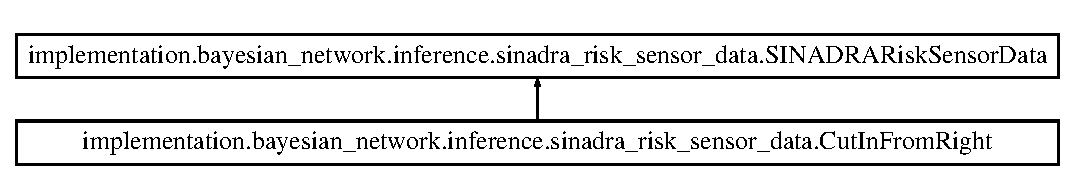
\includegraphics[height=1.989343cm]{classimplementation_1_1bayesian__network_1_1inference_1_1sinadra__risk__sensor__data_1_1_cut_in_from_right}
\end{center}
\end{figure}
\subsection*{Public Member Functions}
\begin{DoxyCompactItemize}
\item 
def \hyperlink{classimplementation_1_1bayesian__network_1_1inference_1_1sinadra__risk__sensor__data_1_1_cut_in_from_right_ab25834a05e23120be3685719bf348155}{\+\_\+\+\_\+init\+\_\+\+\_\+} (self)
\item 
def \hyperlink{classimplementation_1_1bayesian__network_1_1inference_1_1sinadra__risk__sensor__data_1_1_cut_in_from_right_adeae6986decafe9a8ce41ee0dc67d160}{collect\+\_\+data\+\_\+from\+\_\+carla}
\end{DoxyCompactItemize}
\subsection*{Public Attributes}
\begin{DoxyCompactItemize}
\item 
\hyperlink{classimplementation_1_1bayesian__network_1_1inference_1_1sinadra__risk__sensor__data_1_1_cut_in_from_right_a1f80ea1769308a0c801ad2303465b6b6}{vehicle\+\_\+speed}
\item 
\hyperlink{classimplementation_1_1bayesian__network_1_1inference_1_1sinadra__risk__sensor__data_1_1_cut_in_from_right_a71cd808aa4860f4ebf702f52f6aefcf4}{vehicle\+\_\+length}
\item 
\hyperlink{classimplementation_1_1bayesian__network_1_1inference_1_1sinadra__risk__sensor__data_1_1_cut_in_from_right_aedc78a874c889b710f423be888bd9518}{is\+\_\+raining\+\_\+heavy}
\item 
\hyperlink{classimplementation_1_1bayesian__network_1_1inference_1_1sinadra__risk__sensor__data_1_1_cut_in_from_right_a97a6da53108a6f1b64daafd1da252633}{is\+\_\+indicating\+\_\+lane\+\_\+change}
\item 
\hyperlink{classimplementation_1_1bayesian__network_1_1inference_1_1sinadra__risk__sensor__data_1_1_cut_in_from_right_a8e8e8d85994310cb772ade4e02aa7919}{distance\+\_\+to\+\_\+lane\+\_\+end}
\item 
\hyperlink{classimplementation_1_1bayesian__network_1_1inference_1_1sinadra__risk__sensor__data_1_1_cut_in_from_right_a755194128c1ecb73af5207a45bb4216f}{left\+\_\+cut\+\_\+in\+\_\+gap\+\_\+size}
\item 
\hyperlink{classimplementation_1_1bayesian__network_1_1inference_1_1sinadra__risk__sensor__data_1_1_cut_in_from_right_a973c960f32fb5c4996f6db101be1c7a8}{steering\+\_\+angle\+\_\+from\+\_\+lane\+\_\+following}
\item 
\hyperlink{classimplementation_1_1bayesian__network_1_1inference_1_1sinadra__risk__sensor__data_1_1_cut_in_from_right_ad62730db940214cea18286cf9355060f}{distance\+\_\+from\+\_\+left\+\_\+lane\+\_\+line}
\item 
\hyperlink{classimplementation_1_1bayesian__network_1_1inference_1_1sinadra__risk__sensor__data_1_1_cut_in_from_right_a3fd164c3b4eff9b1568de53366b39e06}{distance\+\_\+from\+\_\+lane\+\_\+center}
\end{DoxyCompactItemize}


\subsection{Constructor \& Destructor Documentation}
\mbox{\Hypertarget{classimplementation_1_1bayesian__network_1_1inference_1_1sinadra__risk__sensor__data_1_1_cut_in_from_right_ab25834a05e23120be3685719bf348155}\label{classimplementation_1_1bayesian__network_1_1inference_1_1sinadra__risk__sensor__data_1_1_cut_in_from_right_ab25834a05e23120be3685719bf348155}} 
\index{implementation\+::bayesian\+\_\+network\+::inference\+::sinadra\+\_\+risk\+\_\+sensor\+\_\+data\+::\+Cut\+In\+From\+Right@{implementation\+::bayesian\+\_\+network\+::inference\+::sinadra\+\_\+risk\+\_\+sensor\+\_\+data\+::\+Cut\+In\+From\+Right}!\+\_\+\+\_\+init\+\_\+\+\_\+@{\+\_\+\+\_\+init\+\_\+\+\_\+}}
\index{\+\_\+\+\_\+init\+\_\+\+\_\+@{\+\_\+\+\_\+init\+\_\+\+\_\+}!implementation\+::bayesian\+\_\+network\+::inference\+::sinadra\+\_\+risk\+\_\+sensor\+\_\+data\+::\+Cut\+In\+From\+Right@{implementation\+::bayesian\+\_\+network\+::inference\+::sinadra\+\_\+risk\+\_\+sensor\+\_\+data\+::\+Cut\+In\+From\+Right}}
\subsubsection{\texorpdfstring{\+\_\+\+\_\+init\+\_\+\+\_\+()}{\_\_init\_\_()}}
{\footnotesize\ttfamily def implementation.\+bayesian\+\_\+network.\+inference.\+sinadra\+\_\+risk\+\_\+sensor\+\_\+data.\+Cut\+In\+From\+Right.\+\_\+\+\_\+init\+\_\+\+\_\+ (\begin{DoxyParamCaption}\item[{}]{self }\end{DoxyParamCaption})}



\subsection{Member Function Documentation}
\mbox{\Hypertarget{classimplementation_1_1bayesian__network_1_1inference_1_1sinadra__risk__sensor__data_1_1_cut_in_from_right_adeae6986decafe9a8ce41ee0dc67d160}\label{classimplementation_1_1bayesian__network_1_1inference_1_1sinadra__risk__sensor__data_1_1_cut_in_from_right_adeae6986decafe9a8ce41ee0dc67d160}} 
\index{implementation\+::bayesian\+\_\+network\+::inference\+::sinadra\+\_\+risk\+\_\+sensor\+\_\+data\+::\+Cut\+In\+From\+Right@{implementation\+::bayesian\+\_\+network\+::inference\+::sinadra\+\_\+risk\+\_\+sensor\+\_\+data\+::\+Cut\+In\+From\+Right}!collect\+\_\+data\+\_\+from\+\_\+carla@{collect\+\_\+data\+\_\+from\+\_\+carla}}
\index{collect\+\_\+data\+\_\+from\+\_\+carla@{collect\+\_\+data\+\_\+from\+\_\+carla}!implementation\+::bayesian\+\_\+network\+::inference\+::sinadra\+\_\+risk\+\_\+sensor\+\_\+data\+::\+Cut\+In\+From\+Right@{implementation\+::bayesian\+\_\+network\+::inference\+::sinadra\+\_\+risk\+\_\+sensor\+\_\+data\+::\+Cut\+In\+From\+Right}}
\subsubsection{\texorpdfstring{collect\+\_\+data\+\_\+from\+\_\+carla()}{collect\_data\_from\_carla()}}
{\footnotesize\ttfamily def implementation.\+bayesian\+\_\+network.\+inference.\+sinadra\+\_\+risk\+\_\+sensor\+\_\+data.\+Cut\+In\+From\+Right.\+collect\+\_\+data\+\_\+from\+\_\+carla (\begin{DoxyParamCaption}\item[{}]{self,  }\item[{}]{input\+\_\+feature\+\_\+data }\end{DoxyParamCaption})}



\subsection{Member Data Documentation}
\mbox{\Hypertarget{classimplementation_1_1bayesian__network_1_1inference_1_1sinadra__risk__sensor__data_1_1_cut_in_from_right_a3fd164c3b4eff9b1568de53366b39e06}\label{classimplementation_1_1bayesian__network_1_1inference_1_1sinadra__risk__sensor__data_1_1_cut_in_from_right_a3fd164c3b4eff9b1568de53366b39e06}} 
\index{implementation\+::bayesian\+\_\+network\+::inference\+::sinadra\+\_\+risk\+\_\+sensor\+\_\+data\+::\+Cut\+In\+From\+Right@{implementation\+::bayesian\+\_\+network\+::inference\+::sinadra\+\_\+risk\+\_\+sensor\+\_\+data\+::\+Cut\+In\+From\+Right}!distance\+\_\+from\+\_\+lane\+\_\+center@{distance\+\_\+from\+\_\+lane\+\_\+center}}
\index{distance\+\_\+from\+\_\+lane\+\_\+center@{distance\+\_\+from\+\_\+lane\+\_\+center}!implementation\+::bayesian\+\_\+network\+::inference\+::sinadra\+\_\+risk\+\_\+sensor\+\_\+data\+::\+Cut\+In\+From\+Right@{implementation\+::bayesian\+\_\+network\+::inference\+::sinadra\+\_\+risk\+\_\+sensor\+\_\+data\+::\+Cut\+In\+From\+Right}}
\subsubsection{\texorpdfstring{distance\+\_\+from\+\_\+lane\+\_\+center}{distance\_from\_lane\_center}}
{\footnotesize\ttfamily implementation.\+bayesian\+\_\+network.\+inference.\+sinadra\+\_\+risk\+\_\+sensor\+\_\+data.\+Cut\+In\+From\+Right.\+distance\+\_\+from\+\_\+lane\+\_\+center}

\mbox{\Hypertarget{classimplementation_1_1bayesian__network_1_1inference_1_1sinadra__risk__sensor__data_1_1_cut_in_from_right_ad62730db940214cea18286cf9355060f}\label{classimplementation_1_1bayesian__network_1_1inference_1_1sinadra__risk__sensor__data_1_1_cut_in_from_right_ad62730db940214cea18286cf9355060f}} 
\index{implementation\+::bayesian\+\_\+network\+::inference\+::sinadra\+\_\+risk\+\_\+sensor\+\_\+data\+::\+Cut\+In\+From\+Right@{implementation\+::bayesian\+\_\+network\+::inference\+::sinadra\+\_\+risk\+\_\+sensor\+\_\+data\+::\+Cut\+In\+From\+Right}!distance\+\_\+from\+\_\+left\+\_\+lane\+\_\+line@{distance\+\_\+from\+\_\+left\+\_\+lane\+\_\+line}}
\index{distance\+\_\+from\+\_\+left\+\_\+lane\+\_\+line@{distance\+\_\+from\+\_\+left\+\_\+lane\+\_\+line}!implementation\+::bayesian\+\_\+network\+::inference\+::sinadra\+\_\+risk\+\_\+sensor\+\_\+data\+::\+Cut\+In\+From\+Right@{implementation\+::bayesian\+\_\+network\+::inference\+::sinadra\+\_\+risk\+\_\+sensor\+\_\+data\+::\+Cut\+In\+From\+Right}}
\subsubsection{\texorpdfstring{distance\+\_\+from\+\_\+left\+\_\+lane\+\_\+line}{distance\_from\_left\_lane\_line}}
{\footnotesize\ttfamily implementation.\+bayesian\+\_\+network.\+inference.\+sinadra\+\_\+risk\+\_\+sensor\+\_\+data.\+Cut\+In\+From\+Right.\+distance\+\_\+from\+\_\+left\+\_\+lane\+\_\+line}

\mbox{\Hypertarget{classimplementation_1_1bayesian__network_1_1inference_1_1sinadra__risk__sensor__data_1_1_cut_in_from_right_a8e8e8d85994310cb772ade4e02aa7919}\label{classimplementation_1_1bayesian__network_1_1inference_1_1sinadra__risk__sensor__data_1_1_cut_in_from_right_a8e8e8d85994310cb772ade4e02aa7919}} 
\index{implementation\+::bayesian\+\_\+network\+::inference\+::sinadra\+\_\+risk\+\_\+sensor\+\_\+data\+::\+Cut\+In\+From\+Right@{implementation\+::bayesian\+\_\+network\+::inference\+::sinadra\+\_\+risk\+\_\+sensor\+\_\+data\+::\+Cut\+In\+From\+Right}!distance\+\_\+to\+\_\+lane\+\_\+end@{distance\+\_\+to\+\_\+lane\+\_\+end}}
\index{distance\+\_\+to\+\_\+lane\+\_\+end@{distance\+\_\+to\+\_\+lane\+\_\+end}!implementation\+::bayesian\+\_\+network\+::inference\+::sinadra\+\_\+risk\+\_\+sensor\+\_\+data\+::\+Cut\+In\+From\+Right@{implementation\+::bayesian\+\_\+network\+::inference\+::sinadra\+\_\+risk\+\_\+sensor\+\_\+data\+::\+Cut\+In\+From\+Right}}
\subsubsection{\texorpdfstring{distance\+\_\+to\+\_\+lane\+\_\+end}{distance\_to\_lane\_end}}
{\footnotesize\ttfamily implementation.\+bayesian\+\_\+network.\+inference.\+sinadra\+\_\+risk\+\_\+sensor\+\_\+data.\+Cut\+In\+From\+Right.\+distance\+\_\+to\+\_\+lane\+\_\+end}

\mbox{\Hypertarget{classimplementation_1_1bayesian__network_1_1inference_1_1sinadra__risk__sensor__data_1_1_cut_in_from_right_a97a6da53108a6f1b64daafd1da252633}\label{classimplementation_1_1bayesian__network_1_1inference_1_1sinadra__risk__sensor__data_1_1_cut_in_from_right_a97a6da53108a6f1b64daafd1da252633}} 
\index{implementation\+::bayesian\+\_\+network\+::inference\+::sinadra\+\_\+risk\+\_\+sensor\+\_\+data\+::\+Cut\+In\+From\+Right@{implementation\+::bayesian\+\_\+network\+::inference\+::sinadra\+\_\+risk\+\_\+sensor\+\_\+data\+::\+Cut\+In\+From\+Right}!is\+\_\+indicating\+\_\+lane\+\_\+change@{is\+\_\+indicating\+\_\+lane\+\_\+change}}
\index{is\+\_\+indicating\+\_\+lane\+\_\+change@{is\+\_\+indicating\+\_\+lane\+\_\+change}!implementation\+::bayesian\+\_\+network\+::inference\+::sinadra\+\_\+risk\+\_\+sensor\+\_\+data\+::\+Cut\+In\+From\+Right@{implementation\+::bayesian\+\_\+network\+::inference\+::sinadra\+\_\+risk\+\_\+sensor\+\_\+data\+::\+Cut\+In\+From\+Right}}
\subsubsection{\texorpdfstring{is\+\_\+indicating\+\_\+lane\+\_\+change}{is\_indicating\_lane\_change}}
{\footnotesize\ttfamily implementation.\+bayesian\+\_\+network.\+inference.\+sinadra\+\_\+risk\+\_\+sensor\+\_\+data.\+Cut\+In\+From\+Right.\+is\+\_\+indicating\+\_\+lane\+\_\+change}

\mbox{\Hypertarget{classimplementation_1_1bayesian__network_1_1inference_1_1sinadra__risk__sensor__data_1_1_cut_in_from_right_aedc78a874c889b710f423be888bd9518}\label{classimplementation_1_1bayesian__network_1_1inference_1_1sinadra__risk__sensor__data_1_1_cut_in_from_right_aedc78a874c889b710f423be888bd9518}} 
\index{implementation\+::bayesian\+\_\+network\+::inference\+::sinadra\+\_\+risk\+\_\+sensor\+\_\+data\+::\+Cut\+In\+From\+Right@{implementation\+::bayesian\+\_\+network\+::inference\+::sinadra\+\_\+risk\+\_\+sensor\+\_\+data\+::\+Cut\+In\+From\+Right}!is\+\_\+raining\+\_\+heavy@{is\+\_\+raining\+\_\+heavy}}
\index{is\+\_\+raining\+\_\+heavy@{is\+\_\+raining\+\_\+heavy}!implementation\+::bayesian\+\_\+network\+::inference\+::sinadra\+\_\+risk\+\_\+sensor\+\_\+data\+::\+Cut\+In\+From\+Right@{implementation\+::bayesian\+\_\+network\+::inference\+::sinadra\+\_\+risk\+\_\+sensor\+\_\+data\+::\+Cut\+In\+From\+Right}}
\subsubsection{\texorpdfstring{is\+\_\+raining\+\_\+heavy}{is\_raining\_heavy}}
{\footnotesize\ttfamily implementation.\+bayesian\+\_\+network.\+inference.\+sinadra\+\_\+risk\+\_\+sensor\+\_\+data.\+Cut\+In\+From\+Right.\+is\+\_\+raining\+\_\+heavy}

\mbox{\Hypertarget{classimplementation_1_1bayesian__network_1_1inference_1_1sinadra__risk__sensor__data_1_1_cut_in_from_right_a755194128c1ecb73af5207a45bb4216f}\label{classimplementation_1_1bayesian__network_1_1inference_1_1sinadra__risk__sensor__data_1_1_cut_in_from_right_a755194128c1ecb73af5207a45bb4216f}} 
\index{implementation\+::bayesian\+\_\+network\+::inference\+::sinadra\+\_\+risk\+\_\+sensor\+\_\+data\+::\+Cut\+In\+From\+Right@{implementation\+::bayesian\+\_\+network\+::inference\+::sinadra\+\_\+risk\+\_\+sensor\+\_\+data\+::\+Cut\+In\+From\+Right}!left\+\_\+cut\+\_\+in\+\_\+gap\+\_\+size@{left\+\_\+cut\+\_\+in\+\_\+gap\+\_\+size}}
\index{left\+\_\+cut\+\_\+in\+\_\+gap\+\_\+size@{left\+\_\+cut\+\_\+in\+\_\+gap\+\_\+size}!implementation\+::bayesian\+\_\+network\+::inference\+::sinadra\+\_\+risk\+\_\+sensor\+\_\+data\+::\+Cut\+In\+From\+Right@{implementation\+::bayesian\+\_\+network\+::inference\+::sinadra\+\_\+risk\+\_\+sensor\+\_\+data\+::\+Cut\+In\+From\+Right}}
\subsubsection{\texorpdfstring{left\+\_\+cut\+\_\+in\+\_\+gap\+\_\+size}{left\_cut\_in\_gap\_size}}
{\footnotesize\ttfamily implementation.\+bayesian\+\_\+network.\+inference.\+sinadra\+\_\+risk\+\_\+sensor\+\_\+data.\+Cut\+In\+From\+Right.\+left\+\_\+cut\+\_\+in\+\_\+gap\+\_\+size}

\mbox{\Hypertarget{classimplementation_1_1bayesian__network_1_1inference_1_1sinadra__risk__sensor__data_1_1_cut_in_from_right_a973c960f32fb5c4996f6db101be1c7a8}\label{classimplementation_1_1bayesian__network_1_1inference_1_1sinadra__risk__sensor__data_1_1_cut_in_from_right_a973c960f32fb5c4996f6db101be1c7a8}} 
\index{implementation\+::bayesian\+\_\+network\+::inference\+::sinadra\+\_\+risk\+\_\+sensor\+\_\+data\+::\+Cut\+In\+From\+Right@{implementation\+::bayesian\+\_\+network\+::inference\+::sinadra\+\_\+risk\+\_\+sensor\+\_\+data\+::\+Cut\+In\+From\+Right}!steering\+\_\+angle\+\_\+from\+\_\+lane\+\_\+following@{steering\+\_\+angle\+\_\+from\+\_\+lane\+\_\+following}}
\index{steering\+\_\+angle\+\_\+from\+\_\+lane\+\_\+following@{steering\+\_\+angle\+\_\+from\+\_\+lane\+\_\+following}!implementation\+::bayesian\+\_\+network\+::inference\+::sinadra\+\_\+risk\+\_\+sensor\+\_\+data\+::\+Cut\+In\+From\+Right@{implementation\+::bayesian\+\_\+network\+::inference\+::sinadra\+\_\+risk\+\_\+sensor\+\_\+data\+::\+Cut\+In\+From\+Right}}
\subsubsection{\texorpdfstring{steering\+\_\+angle\+\_\+from\+\_\+lane\+\_\+following}{steering\_angle\_from\_lane\_following}}
{\footnotesize\ttfamily implementation.\+bayesian\+\_\+network.\+inference.\+sinadra\+\_\+risk\+\_\+sensor\+\_\+data.\+Cut\+In\+From\+Right.\+steering\+\_\+angle\+\_\+from\+\_\+lane\+\_\+following}

\mbox{\Hypertarget{classimplementation_1_1bayesian__network_1_1inference_1_1sinadra__risk__sensor__data_1_1_cut_in_from_right_a71cd808aa4860f4ebf702f52f6aefcf4}\label{classimplementation_1_1bayesian__network_1_1inference_1_1sinadra__risk__sensor__data_1_1_cut_in_from_right_a71cd808aa4860f4ebf702f52f6aefcf4}} 
\index{implementation\+::bayesian\+\_\+network\+::inference\+::sinadra\+\_\+risk\+\_\+sensor\+\_\+data\+::\+Cut\+In\+From\+Right@{implementation\+::bayesian\+\_\+network\+::inference\+::sinadra\+\_\+risk\+\_\+sensor\+\_\+data\+::\+Cut\+In\+From\+Right}!vehicle\+\_\+length@{vehicle\+\_\+length}}
\index{vehicle\+\_\+length@{vehicle\+\_\+length}!implementation\+::bayesian\+\_\+network\+::inference\+::sinadra\+\_\+risk\+\_\+sensor\+\_\+data\+::\+Cut\+In\+From\+Right@{implementation\+::bayesian\+\_\+network\+::inference\+::sinadra\+\_\+risk\+\_\+sensor\+\_\+data\+::\+Cut\+In\+From\+Right}}
\subsubsection{\texorpdfstring{vehicle\+\_\+length}{vehicle\_length}}
{\footnotesize\ttfamily implementation.\+bayesian\+\_\+network.\+inference.\+sinadra\+\_\+risk\+\_\+sensor\+\_\+data.\+Cut\+In\+From\+Right.\+vehicle\+\_\+length}

\mbox{\Hypertarget{classimplementation_1_1bayesian__network_1_1inference_1_1sinadra__risk__sensor__data_1_1_cut_in_from_right_a1f80ea1769308a0c801ad2303465b6b6}\label{classimplementation_1_1bayesian__network_1_1inference_1_1sinadra__risk__sensor__data_1_1_cut_in_from_right_a1f80ea1769308a0c801ad2303465b6b6}} 
\index{implementation\+::bayesian\+\_\+network\+::inference\+::sinadra\+\_\+risk\+\_\+sensor\+\_\+data\+::\+Cut\+In\+From\+Right@{implementation\+::bayesian\+\_\+network\+::inference\+::sinadra\+\_\+risk\+\_\+sensor\+\_\+data\+::\+Cut\+In\+From\+Right}!vehicle\+\_\+speed@{vehicle\+\_\+speed}}
\index{vehicle\+\_\+speed@{vehicle\+\_\+speed}!implementation\+::bayesian\+\_\+network\+::inference\+::sinadra\+\_\+risk\+\_\+sensor\+\_\+data\+::\+Cut\+In\+From\+Right@{implementation\+::bayesian\+\_\+network\+::inference\+::sinadra\+\_\+risk\+\_\+sensor\+\_\+data\+::\+Cut\+In\+From\+Right}}
\subsubsection{\texorpdfstring{vehicle\+\_\+speed}{vehicle\_speed}}
{\footnotesize\ttfamily implementation.\+bayesian\+\_\+network.\+inference.\+sinadra\+\_\+risk\+\_\+sensor\+\_\+data.\+Cut\+In\+From\+Right.\+vehicle\+\_\+speed}



The documentation for this class was generated from the following file\+:\begin{DoxyCompactItemize}
\item 
implementation/bayesian\+\_\+network/inference/\hyperlink{sinadra__risk__sensor__data_8py}{sinadra\+\_\+risk\+\_\+sensor\+\_\+data.\+py}\end{DoxyCompactItemize}

\hypertarget{classimplementation_1_1bayesian__network_1_1inference_1_1sinadra__risk__sensor__data_1_1_data1_lane_follow___simple}{}\section{implementation.\+bayesian\+\_\+network.\+inference.\+sinadra\+\_\+risk\+\_\+sensor\+\_\+data.\+Data1\+Lane\+Follow\+\_\+\+Simple Class Reference}
\label{classimplementation_1_1bayesian__network_1_1inference_1_1sinadra__risk__sensor__data_1_1_data1_lane_follow___simple}\index{implementation.\+bayesian\+\_\+network.\+inference.\+sinadra\+\_\+risk\+\_\+sensor\+\_\+data.\+Data1\+Lane\+Follow\+\_\+\+Simple@{implementation.\+bayesian\+\_\+network.\+inference.\+sinadra\+\_\+risk\+\_\+sensor\+\_\+data.\+Data1\+Lane\+Follow\+\_\+\+Simple}}
Inheritance diagram for implementation.\+bayesian\+\_\+network.\+inference.\+sinadra\+\_\+risk\+\_\+sensor\+\_\+data.\+Data1\+Lane\+Follow\+\_\+\+Simple\+:\begin{figure}[H]
\begin{center}
\leavevmode
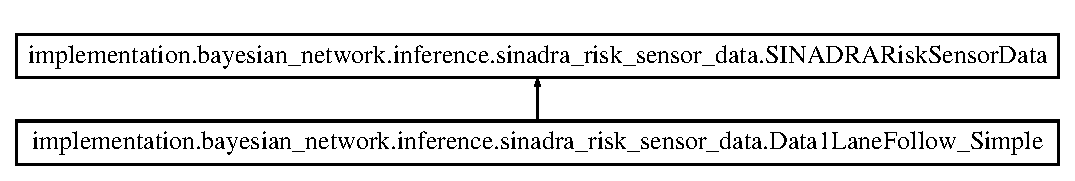
\includegraphics[height=1.989343cm]{classimplementation_1_1bayesian__network_1_1inference_1_1sinadra__risk__sensor__data_1_1_data1_lane_follow___simple}
\end{center}
\end{figure}
\subsection*{Public Member Functions}
\begin{DoxyCompactItemize}
\item 
def \hyperlink{classimplementation_1_1bayesian__network_1_1inference_1_1sinadra__risk__sensor__data_1_1_data1_lane_follow___simple_a7f5f0d89e08e9605ebab8762ad3ab0fd}{\+\_\+\+\_\+init\+\_\+\+\_\+} (self)
\item 
def \hyperlink{classimplementation_1_1bayesian__network_1_1inference_1_1sinadra__risk__sensor__data_1_1_data1_lane_follow___simple_a393e099f3c1cba1f1deddfb5be1b5b94}{collect\+\_\+data\+\_\+from\+\_\+carla}
\end{DoxyCompactItemize}
\subsection*{Public Attributes}
\begin{DoxyCompactItemize}
\item 
\hyperlink{classimplementation_1_1bayesian__network_1_1inference_1_1sinadra__risk__sensor__data_1_1_data1_lane_follow___simple_a209feedf443058990d9cb09e7fefbd34}{is\+\_\+raining\+\_\+heavy}
\item 
\hyperlink{classimplementation_1_1bayesian__network_1_1inference_1_1sinadra__risk__sensor__data_1_1_data1_lane_follow___simple_a4a8855348e29d247d0704fb348567875}{leading\+\_\+vehicle\+\_\+is\+\_\+larger}
\item 
\hyperlink{classimplementation_1_1bayesian__network_1_1inference_1_1sinadra__risk__sensor__data_1_1_data1_lane_follow___simple_ac3cff3aa6903cafb847756a4a7e17b2e}{speed}
\item 
\hyperlink{classimplementation_1_1bayesian__network_1_1inference_1_1sinadra__risk__sensor__data_1_1_data1_lane_follow___simple_a86f235230b034c4e5201580a6b5db49c}{lead\+\_\+vehicle\+\_\+exists}
\item 
\hyperlink{classimplementation_1_1bayesian__network_1_1inference_1_1sinadra__risk__sensor__data_1_1_data1_lane_follow___simple_a87795cd1b68c686c7c4c2998c27fee96}{lead\+\_\+speed}
\item 
\hyperlink{classimplementation_1_1bayesian__network_1_1inference_1_1sinadra__risk__sensor__data_1_1_data1_lane_follow___simple_a46fccba30151cb5e700580ed0436c98e}{distance\+\_\+between\+\_\+vehicles}
\end{DoxyCompactItemize}


\subsection{Constructor \& Destructor Documentation}
\mbox{\Hypertarget{classimplementation_1_1bayesian__network_1_1inference_1_1sinadra__risk__sensor__data_1_1_data1_lane_follow___simple_a7f5f0d89e08e9605ebab8762ad3ab0fd}\label{classimplementation_1_1bayesian__network_1_1inference_1_1sinadra__risk__sensor__data_1_1_data1_lane_follow___simple_a7f5f0d89e08e9605ebab8762ad3ab0fd}} 
\index{implementation\+::bayesian\+\_\+network\+::inference\+::sinadra\+\_\+risk\+\_\+sensor\+\_\+data\+::\+Data1\+Lane\+Follow\+\_\+\+Simple@{implementation\+::bayesian\+\_\+network\+::inference\+::sinadra\+\_\+risk\+\_\+sensor\+\_\+data\+::\+Data1\+Lane\+Follow\+\_\+\+Simple}!\+\_\+\+\_\+init\+\_\+\+\_\+@{\+\_\+\+\_\+init\+\_\+\+\_\+}}
\index{\+\_\+\+\_\+init\+\_\+\+\_\+@{\+\_\+\+\_\+init\+\_\+\+\_\+}!implementation\+::bayesian\+\_\+network\+::inference\+::sinadra\+\_\+risk\+\_\+sensor\+\_\+data\+::\+Data1\+Lane\+Follow\+\_\+\+Simple@{implementation\+::bayesian\+\_\+network\+::inference\+::sinadra\+\_\+risk\+\_\+sensor\+\_\+data\+::\+Data1\+Lane\+Follow\+\_\+\+Simple}}
\subsubsection{\texorpdfstring{\+\_\+\+\_\+init\+\_\+\+\_\+()}{\_\_init\_\_()}}
{\footnotesize\ttfamily def implementation.\+bayesian\+\_\+network.\+inference.\+sinadra\+\_\+risk\+\_\+sensor\+\_\+data.\+Data1\+Lane\+Follow\+\_\+\+Simple.\+\_\+\+\_\+init\+\_\+\+\_\+ (\begin{DoxyParamCaption}\item[{}]{self }\end{DoxyParamCaption})}



\subsection{Member Function Documentation}
\mbox{\Hypertarget{classimplementation_1_1bayesian__network_1_1inference_1_1sinadra__risk__sensor__data_1_1_data1_lane_follow___simple_a393e099f3c1cba1f1deddfb5be1b5b94}\label{classimplementation_1_1bayesian__network_1_1inference_1_1sinadra__risk__sensor__data_1_1_data1_lane_follow___simple_a393e099f3c1cba1f1deddfb5be1b5b94}} 
\index{implementation\+::bayesian\+\_\+network\+::inference\+::sinadra\+\_\+risk\+\_\+sensor\+\_\+data\+::\+Data1\+Lane\+Follow\+\_\+\+Simple@{implementation\+::bayesian\+\_\+network\+::inference\+::sinadra\+\_\+risk\+\_\+sensor\+\_\+data\+::\+Data1\+Lane\+Follow\+\_\+\+Simple}!collect\+\_\+data\+\_\+from\+\_\+carla@{collect\+\_\+data\+\_\+from\+\_\+carla}}
\index{collect\+\_\+data\+\_\+from\+\_\+carla@{collect\+\_\+data\+\_\+from\+\_\+carla}!implementation\+::bayesian\+\_\+network\+::inference\+::sinadra\+\_\+risk\+\_\+sensor\+\_\+data\+::\+Data1\+Lane\+Follow\+\_\+\+Simple@{implementation\+::bayesian\+\_\+network\+::inference\+::sinadra\+\_\+risk\+\_\+sensor\+\_\+data\+::\+Data1\+Lane\+Follow\+\_\+\+Simple}}
\subsubsection{\texorpdfstring{collect\+\_\+data\+\_\+from\+\_\+carla()}{collect\_data\_from\_carla()}}
{\footnotesize\ttfamily def implementation.\+bayesian\+\_\+network.\+inference.\+sinadra\+\_\+risk\+\_\+sensor\+\_\+data.\+Data1\+Lane\+Follow\+\_\+\+Simple.\+collect\+\_\+data\+\_\+from\+\_\+carla (\begin{DoxyParamCaption}\item[{}]{self,  }\item[{}]{input\+\_\+feature\+\_\+data }\end{DoxyParamCaption})}



\subsection{Member Data Documentation}
\mbox{\Hypertarget{classimplementation_1_1bayesian__network_1_1inference_1_1sinadra__risk__sensor__data_1_1_data1_lane_follow___simple_a46fccba30151cb5e700580ed0436c98e}\label{classimplementation_1_1bayesian__network_1_1inference_1_1sinadra__risk__sensor__data_1_1_data1_lane_follow___simple_a46fccba30151cb5e700580ed0436c98e}} 
\index{implementation\+::bayesian\+\_\+network\+::inference\+::sinadra\+\_\+risk\+\_\+sensor\+\_\+data\+::\+Data1\+Lane\+Follow\+\_\+\+Simple@{implementation\+::bayesian\+\_\+network\+::inference\+::sinadra\+\_\+risk\+\_\+sensor\+\_\+data\+::\+Data1\+Lane\+Follow\+\_\+\+Simple}!distance\+\_\+between\+\_\+vehicles@{distance\+\_\+between\+\_\+vehicles}}
\index{distance\+\_\+between\+\_\+vehicles@{distance\+\_\+between\+\_\+vehicles}!implementation\+::bayesian\+\_\+network\+::inference\+::sinadra\+\_\+risk\+\_\+sensor\+\_\+data\+::\+Data1\+Lane\+Follow\+\_\+\+Simple@{implementation\+::bayesian\+\_\+network\+::inference\+::sinadra\+\_\+risk\+\_\+sensor\+\_\+data\+::\+Data1\+Lane\+Follow\+\_\+\+Simple}}
\subsubsection{\texorpdfstring{distance\+\_\+between\+\_\+vehicles}{distance\_between\_vehicles}}
{\footnotesize\ttfamily implementation.\+bayesian\+\_\+network.\+inference.\+sinadra\+\_\+risk\+\_\+sensor\+\_\+data.\+Data1\+Lane\+Follow\+\_\+\+Simple.\+distance\+\_\+between\+\_\+vehicles}

\mbox{\Hypertarget{classimplementation_1_1bayesian__network_1_1inference_1_1sinadra__risk__sensor__data_1_1_data1_lane_follow___simple_a209feedf443058990d9cb09e7fefbd34}\label{classimplementation_1_1bayesian__network_1_1inference_1_1sinadra__risk__sensor__data_1_1_data1_lane_follow___simple_a209feedf443058990d9cb09e7fefbd34}} 
\index{implementation\+::bayesian\+\_\+network\+::inference\+::sinadra\+\_\+risk\+\_\+sensor\+\_\+data\+::\+Data1\+Lane\+Follow\+\_\+\+Simple@{implementation\+::bayesian\+\_\+network\+::inference\+::sinadra\+\_\+risk\+\_\+sensor\+\_\+data\+::\+Data1\+Lane\+Follow\+\_\+\+Simple}!is\+\_\+raining\+\_\+heavy@{is\+\_\+raining\+\_\+heavy}}
\index{is\+\_\+raining\+\_\+heavy@{is\+\_\+raining\+\_\+heavy}!implementation\+::bayesian\+\_\+network\+::inference\+::sinadra\+\_\+risk\+\_\+sensor\+\_\+data\+::\+Data1\+Lane\+Follow\+\_\+\+Simple@{implementation\+::bayesian\+\_\+network\+::inference\+::sinadra\+\_\+risk\+\_\+sensor\+\_\+data\+::\+Data1\+Lane\+Follow\+\_\+\+Simple}}
\subsubsection{\texorpdfstring{is\+\_\+raining\+\_\+heavy}{is\_raining\_heavy}}
{\footnotesize\ttfamily implementation.\+bayesian\+\_\+network.\+inference.\+sinadra\+\_\+risk\+\_\+sensor\+\_\+data.\+Data1\+Lane\+Follow\+\_\+\+Simple.\+is\+\_\+raining\+\_\+heavy}

\mbox{\Hypertarget{classimplementation_1_1bayesian__network_1_1inference_1_1sinadra__risk__sensor__data_1_1_data1_lane_follow___simple_a87795cd1b68c686c7c4c2998c27fee96}\label{classimplementation_1_1bayesian__network_1_1inference_1_1sinadra__risk__sensor__data_1_1_data1_lane_follow___simple_a87795cd1b68c686c7c4c2998c27fee96}} 
\index{implementation\+::bayesian\+\_\+network\+::inference\+::sinadra\+\_\+risk\+\_\+sensor\+\_\+data\+::\+Data1\+Lane\+Follow\+\_\+\+Simple@{implementation\+::bayesian\+\_\+network\+::inference\+::sinadra\+\_\+risk\+\_\+sensor\+\_\+data\+::\+Data1\+Lane\+Follow\+\_\+\+Simple}!lead\+\_\+speed@{lead\+\_\+speed}}
\index{lead\+\_\+speed@{lead\+\_\+speed}!implementation\+::bayesian\+\_\+network\+::inference\+::sinadra\+\_\+risk\+\_\+sensor\+\_\+data\+::\+Data1\+Lane\+Follow\+\_\+\+Simple@{implementation\+::bayesian\+\_\+network\+::inference\+::sinadra\+\_\+risk\+\_\+sensor\+\_\+data\+::\+Data1\+Lane\+Follow\+\_\+\+Simple}}
\subsubsection{\texorpdfstring{lead\+\_\+speed}{lead\_speed}}
{\footnotesize\ttfamily implementation.\+bayesian\+\_\+network.\+inference.\+sinadra\+\_\+risk\+\_\+sensor\+\_\+data.\+Data1\+Lane\+Follow\+\_\+\+Simple.\+lead\+\_\+speed}

\mbox{\Hypertarget{classimplementation_1_1bayesian__network_1_1inference_1_1sinadra__risk__sensor__data_1_1_data1_lane_follow___simple_a86f235230b034c4e5201580a6b5db49c}\label{classimplementation_1_1bayesian__network_1_1inference_1_1sinadra__risk__sensor__data_1_1_data1_lane_follow___simple_a86f235230b034c4e5201580a6b5db49c}} 
\index{implementation\+::bayesian\+\_\+network\+::inference\+::sinadra\+\_\+risk\+\_\+sensor\+\_\+data\+::\+Data1\+Lane\+Follow\+\_\+\+Simple@{implementation\+::bayesian\+\_\+network\+::inference\+::sinadra\+\_\+risk\+\_\+sensor\+\_\+data\+::\+Data1\+Lane\+Follow\+\_\+\+Simple}!lead\+\_\+vehicle\+\_\+exists@{lead\+\_\+vehicle\+\_\+exists}}
\index{lead\+\_\+vehicle\+\_\+exists@{lead\+\_\+vehicle\+\_\+exists}!implementation\+::bayesian\+\_\+network\+::inference\+::sinadra\+\_\+risk\+\_\+sensor\+\_\+data\+::\+Data1\+Lane\+Follow\+\_\+\+Simple@{implementation\+::bayesian\+\_\+network\+::inference\+::sinadra\+\_\+risk\+\_\+sensor\+\_\+data\+::\+Data1\+Lane\+Follow\+\_\+\+Simple}}
\subsubsection{\texorpdfstring{lead\+\_\+vehicle\+\_\+exists}{lead\_vehicle\_exists}}
{\footnotesize\ttfamily implementation.\+bayesian\+\_\+network.\+inference.\+sinadra\+\_\+risk\+\_\+sensor\+\_\+data.\+Data1\+Lane\+Follow\+\_\+\+Simple.\+lead\+\_\+vehicle\+\_\+exists}

\mbox{\Hypertarget{classimplementation_1_1bayesian__network_1_1inference_1_1sinadra__risk__sensor__data_1_1_data1_lane_follow___simple_a4a8855348e29d247d0704fb348567875}\label{classimplementation_1_1bayesian__network_1_1inference_1_1sinadra__risk__sensor__data_1_1_data1_lane_follow___simple_a4a8855348e29d247d0704fb348567875}} 
\index{implementation\+::bayesian\+\_\+network\+::inference\+::sinadra\+\_\+risk\+\_\+sensor\+\_\+data\+::\+Data1\+Lane\+Follow\+\_\+\+Simple@{implementation\+::bayesian\+\_\+network\+::inference\+::sinadra\+\_\+risk\+\_\+sensor\+\_\+data\+::\+Data1\+Lane\+Follow\+\_\+\+Simple}!leading\+\_\+vehicle\+\_\+is\+\_\+larger@{leading\+\_\+vehicle\+\_\+is\+\_\+larger}}
\index{leading\+\_\+vehicle\+\_\+is\+\_\+larger@{leading\+\_\+vehicle\+\_\+is\+\_\+larger}!implementation\+::bayesian\+\_\+network\+::inference\+::sinadra\+\_\+risk\+\_\+sensor\+\_\+data\+::\+Data1\+Lane\+Follow\+\_\+\+Simple@{implementation\+::bayesian\+\_\+network\+::inference\+::sinadra\+\_\+risk\+\_\+sensor\+\_\+data\+::\+Data1\+Lane\+Follow\+\_\+\+Simple}}
\subsubsection{\texorpdfstring{leading\+\_\+vehicle\+\_\+is\+\_\+larger}{leading\_vehicle\_is\_larger}}
{\footnotesize\ttfamily implementation.\+bayesian\+\_\+network.\+inference.\+sinadra\+\_\+risk\+\_\+sensor\+\_\+data.\+Data1\+Lane\+Follow\+\_\+\+Simple.\+leading\+\_\+vehicle\+\_\+is\+\_\+larger}

\mbox{\Hypertarget{classimplementation_1_1bayesian__network_1_1inference_1_1sinadra__risk__sensor__data_1_1_data1_lane_follow___simple_ac3cff3aa6903cafb847756a4a7e17b2e}\label{classimplementation_1_1bayesian__network_1_1inference_1_1sinadra__risk__sensor__data_1_1_data1_lane_follow___simple_ac3cff3aa6903cafb847756a4a7e17b2e}} 
\index{implementation\+::bayesian\+\_\+network\+::inference\+::sinadra\+\_\+risk\+\_\+sensor\+\_\+data\+::\+Data1\+Lane\+Follow\+\_\+\+Simple@{implementation\+::bayesian\+\_\+network\+::inference\+::sinadra\+\_\+risk\+\_\+sensor\+\_\+data\+::\+Data1\+Lane\+Follow\+\_\+\+Simple}!speed@{speed}}
\index{speed@{speed}!implementation\+::bayesian\+\_\+network\+::inference\+::sinadra\+\_\+risk\+\_\+sensor\+\_\+data\+::\+Data1\+Lane\+Follow\+\_\+\+Simple@{implementation\+::bayesian\+\_\+network\+::inference\+::sinadra\+\_\+risk\+\_\+sensor\+\_\+data\+::\+Data1\+Lane\+Follow\+\_\+\+Simple}}
\subsubsection{\texorpdfstring{speed}{speed}}
{\footnotesize\ttfamily implementation.\+bayesian\+\_\+network.\+inference.\+sinadra\+\_\+risk\+\_\+sensor\+\_\+data.\+Data1\+Lane\+Follow\+\_\+\+Simple.\+speed}



The documentation for this class was generated from the following file\+:\begin{DoxyCompactItemize}
\item 
implementation/bayesian\+\_\+network/inference/\hyperlink{sinadra__risk__sensor__data_8py}{sinadra\+\_\+risk\+\_\+sensor\+\_\+data.\+py}\end{DoxyCompactItemize}

\hypertarget{classimplementation_1_1data__model_1_1environment_1_1_date_time}{}\section{implementation.\+data\+\_\+model.\+environment.\+Date\+Time Class Reference}
\label{classimplementation_1_1data__model_1_1environment_1_1_date_time}\index{implementation.\+data\+\_\+model.\+environment.\+Date\+Time@{implementation.\+data\+\_\+model.\+environment.\+Date\+Time}}
\subsection*{Static Public Attributes}
\begin{DoxyCompactItemize}
\item 
\hyperlink{classimplementation_1_1data__model_1_1environment_1_1_date_time_a81f9c53a5b8bebd70a85f3edcc961862}{int}
\end{DoxyCompactItemize}


\subsection{Member Data Documentation}
\mbox{\Hypertarget{classimplementation_1_1data__model_1_1environment_1_1_date_time_a81f9c53a5b8bebd70a85f3edcc961862}\label{classimplementation_1_1data__model_1_1environment_1_1_date_time_a81f9c53a5b8bebd70a85f3edcc961862}} 
\index{implementation\+::data\+\_\+model\+::environment\+::\+Date\+Time@{implementation\+::data\+\_\+model\+::environment\+::\+Date\+Time}!int@{int}}
\index{int@{int}!implementation\+::data\+\_\+model\+::environment\+::\+Date\+Time@{implementation\+::data\+\_\+model\+::environment\+::\+Date\+Time}}
\subsubsection{\texorpdfstring{int}{int}}
{\footnotesize\ttfamily implementation.\+data\+\_\+model.\+environment.\+Date\+Time.\+int\hspace{0.3cm}{\ttfamily [static]}}



The documentation for this class was generated from the following file\+:\begin{DoxyCompactItemize}
\item 
implementation/data\+\_\+model/\hyperlink{environment_8py}{environment.\+py}\end{DoxyCompactItemize}

\hypertarget{classimplementation_1_1data__model_1_1entity_1_1_dimension}{}\section{implementation.\+data\+\_\+model.\+entity.\+Dimension Class Reference}
\label{classimplementation_1_1data__model_1_1entity_1_1_dimension}\index{implementation.\+data\+\_\+model.\+entity.\+Dimension@{implementation.\+data\+\_\+model.\+entity.\+Dimension}}
\subsection*{Static Public Attributes}
\begin{DoxyCompactItemize}
\item 
\hyperlink{classimplementation_1_1data__model_1_1entity_1_1_dimension_a16deb87502aed4dfd49c48ba374c6052}{float}
\end{DoxyCompactItemize}


\subsection{Detailed Description}
\begin{DoxyVerb}Dimensions for a three dimensional box. Width, length and height are the absolute extensions in the
(x, y, z) coordinate system of the entity's local coordinate system

Attributes
----------
length : float
    Length of the entity's bounding box
width : float
    Width of the entity's bounding box
height : float
    Height of the entity's bounding box
\end{DoxyVerb}
 

\subsection{Member Data Documentation}
\mbox{\Hypertarget{classimplementation_1_1data__model_1_1entity_1_1_dimension_a16deb87502aed4dfd49c48ba374c6052}\label{classimplementation_1_1data__model_1_1entity_1_1_dimension_a16deb87502aed4dfd49c48ba374c6052}} 
\index{implementation\+::data\+\_\+model\+::entity\+::\+Dimension@{implementation\+::data\+\_\+model\+::entity\+::\+Dimension}!float@{float}}
\index{float@{float}!implementation\+::data\+\_\+model\+::entity\+::\+Dimension@{implementation\+::data\+\_\+model\+::entity\+::\+Dimension}}
\subsubsection{\texorpdfstring{float}{float}}
{\footnotesize\ttfamily implementation.\+data\+\_\+model.\+entity.\+Dimension.\+float\hspace{0.3cm}{\ttfamily [static]}}



The documentation for this class was generated from the following file\+:\begin{DoxyCompactItemize}
\item 
implementation/data\+\_\+model/\hyperlink{entity_8py}{entity.\+py}\end{DoxyCompactItemize}

\hypertarget{classimplementation_1_1data__model_1_1vehicle_1_1_ego_vehicle}{}\section{implementation.\+data\+\_\+model.\+vehicle.\+Ego\+Vehicle Class Reference}
\label{classimplementation_1_1data__model_1_1vehicle_1_1_ego_vehicle}\index{implementation.\+data\+\_\+model.\+vehicle.\+Ego\+Vehicle@{implementation.\+data\+\_\+model.\+vehicle.\+Ego\+Vehicle}}
Inheritance diagram for implementation.\+data\+\_\+model.\+vehicle.\+Ego\+Vehicle\+:\begin{figure}[H]
\begin{center}
\leavevmode
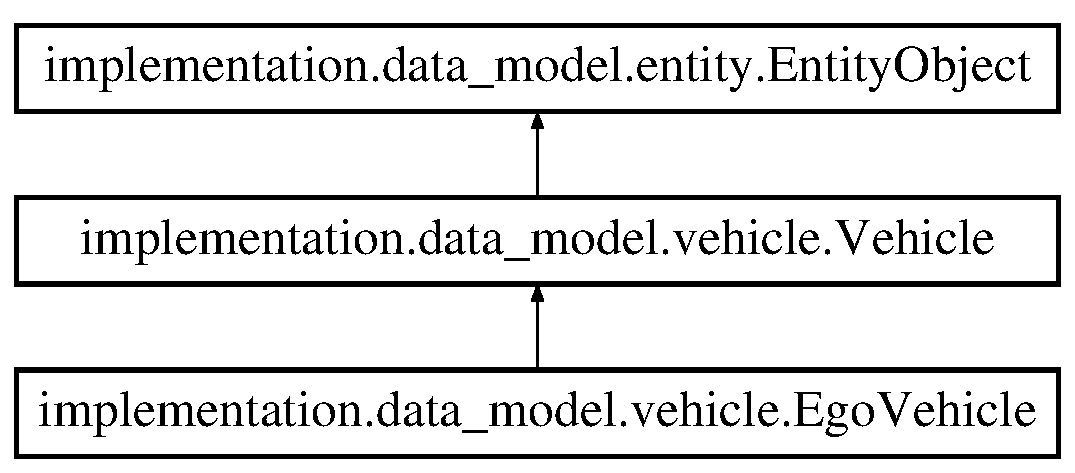
\includegraphics[height=3.000000cm]{classimplementation_1_1data__model_1_1vehicle_1_1_ego_vehicle}
\end{center}
\end{figure}
\subsection*{Public Member Functions}
\begin{DoxyCompactItemize}
\item 
def \hyperlink{classimplementation_1_1data__model_1_1vehicle_1_1_ego_vehicle_ad8165c0170e23589f0c6279ba4f7375d}{get\+\_\+side\+\_\+sensing\+\_\+area}
\item 
def \hyperlink{classimplementation_1_1data__model_1_1vehicle_1_1_ego_vehicle_acf6215a9d5f680822306f8dc785764f5}{get\+\_\+front\+\_\+sensing\+\_\+area} (self, map, Polygon, List, Line\+String)
\end{DoxyCompactItemize}
\subsection*{Additional Inherited Members}


\subsection{Member Function Documentation}
\mbox{\Hypertarget{classimplementation_1_1data__model_1_1vehicle_1_1_ego_vehicle_acf6215a9d5f680822306f8dc785764f5}\label{classimplementation_1_1data__model_1_1vehicle_1_1_ego_vehicle_acf6215a9d5f680822306f8dc785764f5}} 
\index{implementation\+::data\+\_\+model\+::vehicle\+::\+Ego\+Vehicle@{implementation\+::data\+\_\+model\+::vehicle\+::\+Ego\+Vehicle}!get\+\_\+front\+\_\+sensing\+\_\+area@{get\+\_\+front\+\_\+sensing\+\_\+area}}
\index{get\+\_\+front\+\_\+sensing\+\_\+area@{get\+\_\+front\+\_\+sensing\+\_\+area}!implementation\+::data\+\_\+model\+::vehicle\+::\+Ego\+Vehicle@{implementation\+::data\+\_\+model\+::vehicle\+::\+Ego\+Vehicle}}
\subsubsection{\texorpdfstring{get\+\_\+front\+\_\+sensing\+\_\+area()}{get\_front\_sensing\_area()}}
{\footnotesize\ttfamily def implementation.\+data\+\_\+model.\+vehicle.\+Ego\+Vehicle.\+get\+\_\+front\+\_\+sensing\+\_\+area (\begin{DoxyParamCaption}\item[{}]{self,  }\item[{}]{map,  }\item[{}]{Polygon,  }\item[{}]{List,  }\item[{}]{Line\+String }\end{DoxyParamCaption})}

\begin{DoxyVerb}Determines front sensing area for this vehicle using the configuration parameter
FRONT_SENSING_DISTANCE_TIME_GAP_IN_SECONDS. Returns front sensing area as shapely.geometry.Polygon object.
If configuration parameter DEBUG_MODE is set to true, this method additionally returns the lines of the polygon
as a list of shapely.geometry.LineString objects for visualization in carla.

Parameters
----------
map: Map
    Map object to obtain points for sensing area calculation

Returns
-------
Polygon
    A shapely.geometry.Polygon object that defines the front sensing area
List[LineString]
    A list of shapely.geometry.LineString objects that represent the edges of the front sensing area.
    The line strings are only needed for drawing debug lines of the sensing area on the Carla server. Therefore
    the list is only returned if DEBUG_MODE flag is set to True. Otherwise None is returned instead.
\end{DoxyVerb}
 \mbox{\Hypertarget{classimplementation_1_1data__model_1_1vehicle_1_1_ego_vehicle_ad8165c0170e23589f0c6279ba4f7375d}\label{classimplementation_1_1data__model_1_1vehicle_1_1_ego_vehicle_ad8165c0170e23589f0c6279ba4f7375d}} 
\index{implementation\+::data\+\_\+model\+::vehicle\+::\+Ego\+Vehicle@{implementation\+::data\+\_\+model\+::vehicle\+::\+Ego\+Vehicle}!get\+\_\+side\+\_\+sensing\+\_\+area@{get\+\_\+side\+\_\+sensing\+\_\+area}}
\index{get\+\_\+side\+\_\+sensing\+\_\+area@{get\+\_\+side\+\_\+sensing\+\_\+area}!implementation\+::data\+\_\+model\+::vehicle\+::\+Ego\+Vehicle@{implementation\+::data\+\_\+model\+::vehicle\+::\+Ego\+Vehicle}}
\subsubsection{\texorpdfstring{get\+\_\+side\+\_\+sensing\+\_\+area()}{get\_side\_sensing\_area()}}
{\footnotesize\ttfamily def implementation.\+data\+\_\+model.\+vehicle.\+Ego\+Vehicle.\+get\+\_\+side\+\_\+sensing\+\_\+area (\begin{DoxyParamCaption}\item[{}]{self,  }\item[{}]{map }\end{DoxyParamCaption})}



The documentation for this class was generated from the following file\+:\begin{DoxyCompactItemize}
\item 
implementation/data\+\_\+model/\hyperlink{vehicle_8py}{vehicle.\+py}\end{DoxyCompactItemize}

\hypertarget{classimplementation_1_1data__model_1_1entity_1_1_entity_object}{}\section{implementation.\+data\+\_\+model.\+entity.\+Entity\+Object Class Reference}
\label{classimplementation_1_1data__model_1_1entity_1_1_entity_object}\index{implementation.\+data\+\_\+model.\+entity.\+Entity\+Object@{implementation.\+data\+\_\+model.\+entity.\+Entity\+Object}}
Inheritance diagram for implementation.\+data\+\_\+model.\+entity.\+Entity\+Object\+:\begin{figure}[H]
\begin{center}
\leavevmode
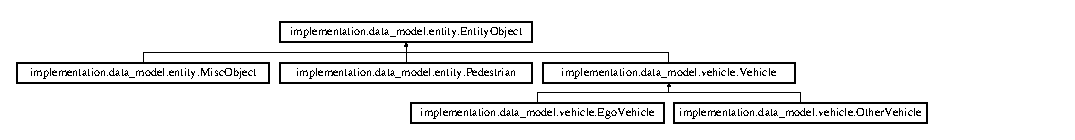
\includegraphics[height=1.428571cm]{classimplementation_1_1data__model_1_1entity_1_1_entity_object}
\end{center}
\end{figure}
\subsection*{Public Member Functions}
\begin{DoxyCompactItemize}
\item 
def \hyperlink{classimplementation_1_1data__model_1_1entity_1_1_entity_object_a5daf332215d128db4067cb3d57708fd7}{get\+\_\+location} (self)
\item 
def \hyperlink{classimplementation_1_1data__model_1_1entity_1_1_entity_object_af4e061592d0d6ee3d191faace28ab781}{get\+\_\+orientation} (self)
\item 
def \hyperlink{classimplementation_1_1data__model_1_1entity_1_1_entity_object_a13695fb863c4e98d2c391f70a8373637}{get\+\_\+world\+\_\+position} (self)
\end{DoxyCompactItemize}
\subsection*{Static Public Attributes}
\begin{DoxyCompactItemize}
\item 
\hyperlink{classimplementation_1_1data__model_1_1entity_1_1_entity_object_a7ddc178ef36e8b94018411edb5ea62be}{str}
\item 
\hyperlink{classimplementation_1_1data__model_1_1entity_1_1_entity_object_a07c9819804b2d844354ba54ca1ccd563}{Position}
\item 
\hyperlink{classimplementation_1_1data__model_1_1entity_1_1_entity_object_a83e7ce8061eee760273dc616d92fb54d}{Bounding\+Box}
\end{DoxyCompactItemize}


\subsection{Detailed Description}
\begin{DoxyVerb}A vehicle type, pedestrian type or miscellaneous object type

 Attributes
 ----------
 name : str
    Name of the Entity
mass : Optional[float]
    The mass of the object in kg
position : Position
    Position object of the Entity
bounding_box : BoundingBox
    The three dimensional bounding box that encloses the vehicle
\end{DoxyVerb}
 

\subsection{Member Function Documentation}
\mbox{\Hypertarget{classimplementation_1_1data__model_1_1entity_1_1_entity_object_a5daf332215d128db4067cb3d57708fd7}\label{classimplementation_1_1data__model_1_1entity_1_1_entity_object_a5daf332215d128db4067cb3d57708fd7}} 
\index{implementation\+::data\+\_\+model\+::entity\+::\+Entity\+Object@{implementation\+::data\+\_\+model\+::entity\+::\+Entity\+Object}!get\+\_\+location@{get\+\_\+location}}
\index{get\+\_\+location@{get\+\_\+location}!implementation\+::data\+\_\+model\+::entity\+::\+Entity\+Object@{implementation\+::data\+\_\+model\+::entity\+::\+Entity\+Object}}
\subsubsection{\texorpdfstring{get\+\_\+location()}{get\_location()}}
{\footnotesize\ttfamily def implementation.\+data\+\_\+model.\+entity.\+Entity\+Object.\+get\+\_\+location (\begin{DoxyParamCaption}\item[{}]{self,  }\item[{}]{Location }\end{DoxyParamCaption})}

\begin{DoxyVerb}Returns the location of the entity in world coordinates.

Returns
-------
Location
    Location of the entity in world coordinates
\end{DoxyVerb}
 \mbox{\Hypertarget{classimplementation_1_1data__model_1_1entity_1_1_entity_object_af4e061592d0d6ee3d191faace28ab781}\label{classimplementation_1_1data__model_1_1entity_1_1_entity_object_af4e061592d0d6ee3d191faace28ab781}} 
\index{implementation\+::data\+\_\+model\+::entity\+::\+Entity\+Object@{implementation\+::data\+\_\+model\+::entity\+::\+Entity\+Object}!get\+\_\+orientation@{get\+\_\+orientation}}
\index{get\+\_\+orientation@{get\+\_\+orientation}!implementation\+::data\+\_\+model\+::entity\+::\+Entity\+Object@{implementation\+::data\+\_\+model\+::entity\+::\+Entity\+Object}}
\subsubsection{\texorpdfstring{get\+\_\+orientation()}{get\_orientation()}}
{\footnotesize\ttfamily def implementation.\+data\+\_\+model.\+entity.\+Entity\+Object.\+get\+\_\+orientation (\begin{DoxyParamCaption}\item[{}]{self,  }\item[{}]{Orientation }\end{DoxyParamCaption})}

\begin{DoxyVerb}Returns the orientation of the entity in world coordinates.

Returns
-------
Orientation
    Orientation of the entity in world coordinates
\end{DoxyVerb}
 \mbox{\Hypertarget{classimplementation_1_1data__model_1_1entity_1_1_entity_object_a13695fb863c4e98d2c391f70a8373637}\label{classimplementation_1_1data__model_1_1entity_1_1_entity_object_a13695fb863c4e98d2c391f70a8373637}} 
\index{implementation\+::data\+\_\+model\+::entity\+::\+Entity\+Object@{implementation\+::data\+\_\+model\+::entity\+::\+Entity\+Object}!get\+\_\+world\+\_\+position@{get\+\_\+world\+\_\+position}}
\index{get\+\_\+world\+\_\+position@{get\+\_\+world\+\_\+position}!implementation\+::data\+\_\+model\+::entity\+::\+Entity\+Object@{implementation\+::data\+\_\+model\+::entity\+::\+Entity\+Object}}
\subsubsection{\texorpdfstring{get\+\_\+world\+\_\+position()}{get\_world\_position()}}
{\footnotesize\ttfamily def implementation.\+data\+\_\+model.\+entity.\+Entity\+Object.\+get\+\_\+world\+\_\+position (\begin{DoxyParamCaption}\item[{}]{self,  }\item[{}]{World\+Position }\end{DoxyParamCaption})}

\begin{DoxyVerb}Returns the world position of the entity in world coordinates.

Returns
-------
WorldPosition
    WorldPosition of the entity in world coordinates
\end{DoxyVerb}
 

\subsection{Member Data Documentation}
\mbox{\Hypertarget{classimplementation_1_1data__model_1_1entity_1_1_entity_object_a83e7ce8061eee760273dc616d92fb54d}\label{classimplementation_1_1data__model_1_1entity_1_1_entity_object_a83e7ce8061eee760273dc616d92fb54d}} 
\index{implementation\+::data\+\_\+model\+::entity\+::\+Entity\+Object@{implementation\+::data\+\_\+model\+::entity\+::\+Entity\+Object}!Bounding\+Box@{Bounding\+Box}}
\index{Bounding\+Box@{Bounding\+Box}!implementation\+::data\+\_\+model\+::entity\+::\+Entity\+Object@{implementation\+::data\+\_\+model\+::entity\+::\+Entity\+Object}}
\subsubsection{\texorpdfstring{Bounding\+Box}{BoundingBox}}
{\footnotesize\ttfamily implementation.\+data\+\_\+model.\+entity.\+Entity\+Object.\+Bounding\+Box\hspace{0.3cm}{\ttfamily [static]}}

\mbox{\Hypertarget{classimplementation_1_1data__model_1_1entity_1_1_entity_object_a07c9819804b2d844354ba54ca1ccd563}\label{classimplementation_1_1data__model_1_1entity_1_1_entity_object_a07c9819804b2d844354ba54ca1ccd563}} 
\index{implementation\+::data\+\_\+model\+::entity\+::\+Entity\+Object@{implementation\+::data\+\_\+model\+::entity\+::\+Entity\+Object}!Position@{Position}}
\index{Position@{Position}!implementation\+::data\+\_\+model\+::entity\+::\+Entity\+Object@{implementation\+::data\+\_\+model\+::entity\+::\+Entity\+Object}}
\subsubsection{\texorpdfstring{Position}{Position}}
{\footnotesize\ttfamily implementation.\+data\+\_\+model.\+entity.\+Entity\+Object.\+Position\hspace{0.3cm}{\ttfamily [static]}}

\mbox{\Hypertarget{classimplementation_1_1data__model_1_1entity_1_1_entity_object_a7ddc178ef36e8b94018411edb5ea62be}\label{classimplementation_1_1data__model_1_1entity_1_1_entity_object_a7ddc178ef36e8b94018411edb5ea62be}} 
\index{implementation\+::data\+\_\+model\+::entity\+::\+Entity\+Object@{implementation\+::data\+\_\+model\+::entity\+::\+Entity\+Object}!str@{str}}
\index{str@{str}!implementation\+::data\+\_\+model\+::entity\+::\+Entity\+Object@{implementation\+::data\+\_\+model\+::entity\+::\+Entity\+Object}}
\subsubsection{\texorpdfstring{str}{str}}
{\footnotesize\ttfamily implementation.\+data\+\_\+model.\+entity.\+Entity\+Object.\+str\hspace{0.3cm}{\ttfamily [static]}}



The documentation for this class was generated from the following file\+:\begin{DoxyCompactItemize}
\item 
implementation/data\+\_\+model/\hyperlink{entity_8py}{entity.\+py}\end{DoxyCompactItemize}

\hypertarget{classimplementation_1_1data__model_1_1environment_1_1_environment}{}\section{implementation.\+data\+\_\+model.\+environment.\+Environment Class Reference}
\label{classimplementation_1_1data__model_1_1environment_1_1_environment}\index{implementation.\+data\+\_\+model.\+environment.\+Environment@{implementation.\+data\+\_\+model.\+environment.\+Environment}}
\subsection*{Static Public Attributes}
\begin{DoxyCompactItemize}
\item 
\hyperlink{classimplementation_1_1data__model_1_1environment_1_1_environment_a8ae9a68fead7ddcdf8b34193848ae53d}{str}
\end{DoxyCompactItemize}


\subsection{Member Data Documentation}
\mbox{\Hypertarget{classimplementation_1_1data__model_1_1environment_1_1_environment_a8ae9a68fead7ddcdf8b34193848ae53d}\label{classimplementation_1_1data__model_1_1environment_1_1_environment_a8ae9a68fead7ddcdf8b34193848ae53d}} 
\index{implementation\+::data\+\_\+model\+::environment\+::\+Environment@{implementation\+::data\+\_\+model\+::environment\+::\+Environment}!str@{str}}
\index{str@{str}!implementation\+::data\+\_\+model\+::environment\+::\+Environment@{implementation\+::data\+\_\+model\+::environment\+::\+Environment}}
\subsubsection{\texorpdfstring{str}{str}}
{\footnotesize\ttfamily implementation.\+data\+\_\+model.\+environment.\+Environment.\+str\hspace{0.3cm}{\ttfamily [static]}}



The documentation for this class was generated from the following file\+:\begin{DoxyCompactItemize}
\item 
implementation/data\+\_\+model/\hyperlink{environment_8py}{environment.\+py}\end{DoxyCompactItemize}

\hypertarget{classimplementation_1_1manual__control_1_1_fading_text}{}\doxysection{implementation.\+manual\+\_\+control.\+Fading\+Text Class Reference}
\label{classimplementation_1_1manual__control_1_1_fading_text}\index{implementation.manual\_control.FadingText@{implementation.manual\_control.FadingText}}
Inheritance diagram for implementation.\+manual\+\_\+control.\+Fading\+Text\+:\begin{figure}[H]
\begin{center}
\leavevmode
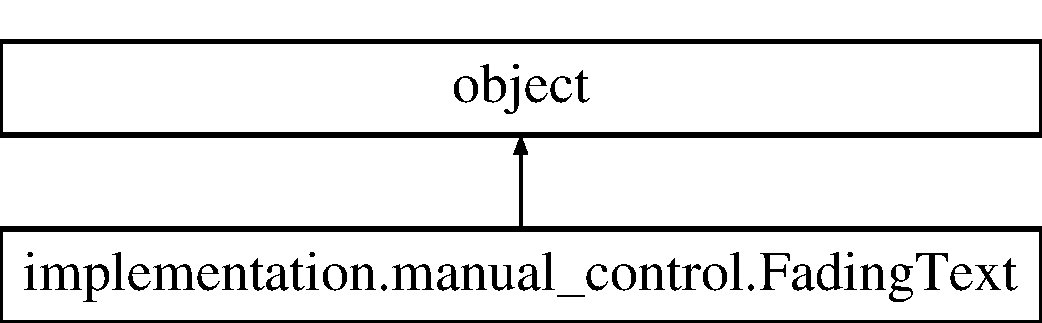
\includegraphics[height=2.000000cm]{classimplementation_1_1manual__control_1_1_fading_text}
\end{center}
\end{figure}
\doxysubsection*{Public Member Functions}
\begin{DoxyCompactItemize}
\item 
def \mbox{\hyperlink{classimplementation_1_1manual__control_1_1_fading_text_a53de3cc3e5cf3e7f33e0d8e58dcf5a65}{\+\_\+\+\_\+init\+\_\+\+\_\+}} (self, \mbox{\hyperlink{classimplementation_1_1manual__control_1_1_fading_text_a082fb4699489a87bdbacb57c98c12b03}{font}}, \mbox{\hyperlink{classimplementation_1_1manual__control_1_1_fading_text_a0f27882c9976418cb316d18dfb6fdfa0}{dim}}, \mbox{\hyperlink{classimplementation_1_1manual__control_1_1_fading_text_a37bc572c9faf6b8d5803e5a52bda25b7}{pos}})
\item 
def \mbox{\hyperlink{classimplementation_1_1manual__control_1_1_fading_text_a8c4b42f518a578286bacb5bc0f8988ae}{set\+\_\+text}} (self, text, color=(255, 255, 255), seconds=2.\+0)
\item 
def \mbox{\hyperlink{classimplementation_1_1manual__control_1_1_fading_text_a1b6d98594b0a590e8333ab2dd6523d09}{tick}} (self, \+\_\+, clock)
\item 
def \mbox{\hyperlink{classimplementation_1_1manual__control_1_1_fading_text_ac40469e99420d5e9c62a1dbcce7f4c01}{render}} (self, display)
\end{DoxyCompactItemize}
\doxysubsection*{Public Attributes}
\begin{DoxyCompactItemize}
\item 
\mbox{\hyperlink{classimplementation_1_1manual__control_1_1_fading_text_a082fb4699489a87bdbacb57c98c12b03}{font}}
\item 
\mbox{\hyperlink{classimplementation_1_1manual__control_1_1_fading_text_a0f27882c9976418cb316d18dfb6fdfa0}{dim}}
\item 
\mbox{\hyperlink{classimplementation_1_1manual__control_1_1_fading_text_a37bc572c9faf6b8d5803e5a52bda25b7}{pos}}
\item 
\mbox{\hyperlink{classimplementation_1_1manual__control_1_1_fading_text_ac656b26edb4bfadbdd58e823d9500aeb}{seconds\+\_\+left}}
\item 
\mbox{\hyperlink{classimplementation_1_1manual__control_1_1_fading_text_a7c817f00bbeae6e99ca1079405516866}{surface}}
\end{DoxyCompactItemize}


\doxysubsection{Constructor \& Destructor Documentation}
\mbox{\Hypertarget{classimplementation_1_1manual__control_1_1_fading_text_a53de3cc3e5cf3e7f33e0d8e58dcf5a65}\label{classimplementation_1_1manual__control_1_1_fading_text_a53de3cc3e5cf3e7f33e0d8e58dcf5a65}} 
\index{implementation.manual\_control.FadingText@{implementation.manual\_control.FadingText}!\_\_init\_\_@{\_\_init\_\_}}
\index{\_\_init\_\_@{\_\_init\_\_}!implementation.manual\_control.FadingText@{implementation.manual\_control.FadingText}}
\doxysubsubsection{\texorpdfstring{\_\_init\_\_()}{\_\_init\_\_()}}
{\footnotesize\ttfamily def implementation.\+manual\+\_\+control.\+Fading\+Text.\+\_\+\+\_\+init\+\_\+\+\_\+ (\begin{DoxyParamCaption}\item[{}]{self,  }\item[{}]{font,  }\item[{}]{dim,  }\item[{}]{pos }\end{DoxyParamCaption})}



\doxysubsection{Member Function Documentation}
\mbox{\Hypertarget{classimplementation_1_1manual__control_1_1_fading_text_ac40469e99420d5e9c62a1dbcce7f4c01}\label{classimplementation_1_1manual__control_1_1_fading_text_ac40469e99420d5e9c62a1dbcce7f4c01}} 
\index{implementation.manual\_control.FadingText@{implementation.manual\_control.FadingText}!render@{render}}
\index{render@{render}!implementation.manual\_control.FadingText@{implementation.manual\_control.FadingText}}
\doxysubsubsection{\texorpdfstring{render()}{render()}}
{\footnotesize\ttfamily def implementation.\+manual\+\_\+control.\+Fading\+Text.\+render (\begin{DoxyParamCaption}\item[{}]{self,  }\item[{}]{display }\end{DoxyParamCaption})}

\mbox{\Hypertarget{classimplementation_1_1manual__control_1_1_fading_text_a8c4b42f518a578286bacb5bc0f8988ae}\label{classimplementation_1_1manual__control_1_1_fading_text_a8c4b42f518a578286bacb5bc0f8988ae}} 
\index{implementation.manual\_control.FadingText@{implementation.manual\_control.FadingText}!set\_text@{set\_text}}
\index{set\_text@{set\_text}!implementation.manual\_control.FadingText@{implementation.manual\_control.FadingText}}
\doxysubsubsection{\texorpdfstring{set\_text()}{set\_text()}}
{\footnotesize\ttfamily def implementation.\+manual\+\_\+control.\+Fading\+Text.\+set\+\_\+text (\begin{DoxyParamCaption}\item[{}]{self,  }\item[{}]{text,  }\item[{}]{color = {\ttfamily (255,~255,~255)},  }\item[{}]{seconds = {\ttfamily 2.0} }\end{DoxyParamCaption})}

\mbox{\Hypertarget{classimplementation_1_1manual__control_1_1_fading_text_a1b6d98594b0a590e8333ab2dd6523d09}\label{classimplementation_1_1manual__control_1_1_fading_text_a1b6d98594b0a590e8333ab2dd6523d09}} 
\index{implementation.manual\_control.FadingText@{implementation.manual\_control.FadingText}!tick@{tick}}
\index{tick@{tick}!implementation.manual\_control.FadingText@{implementation.manual\_control.FadingText}}
\doxysubsubsection{\texorpdfstring{tick()}{tick()}}
{\footnotesize\ttfamily def implementation.\+manual\+\_\+control.\+Fading\+Text.\+tick (\begin{DoxyParamCaption}\item[{}]{self,  }\item[{}]{\+\_\+,  }\item[{}]{clock }\end{DoxyParamCaption})}



\doxysubsection{Member Data Documentation}
\mbox{\Hypertarget{classimplementation_1_1manual__control_1_1_fading_text_a0f27882c9976418cb316d18dfb6fdfa0}\label{classimplementation_1_1manual__control_1_1_fading_text_a0f27882c9976418cb316d18dfb6fdfa0}} 
\index{implementation.manual\_control.FadingText@{implementation.manual\_control.FadingText}!dim@{dim}}
\index{dim@{dim}!implementation.manual\_control.FadingText@{implementation.manual\_control.FadingText}}
\doxysubsubsection{\texorpdfstring{dim}{dim}}
{\footnotesize\ttfamily implementation.\+manual\+\_\+control.\+Fading\+Text.\+dim}

\mbox{\Hypertarget{classimplementation_1_1manual__control_1_1_fading_text_a082fb4699489a87bdbacb57c98c12b03}\label{classimplementation_1_1manual__control_1_1_fading_text_a082fb4699489a87bdbacb57c98c12b03}} 
\index{implementation.manual\_control.FadingText@{implementation.manual\_control.FadingText}!font@{font}}
\index{font@{font}!implementation.manual\_control.FadingText@{implementation.manual\_control.FadingText}}
\doxysubsubsection{\texorpdfstring{font}{font}}
{\footnotesize\ttfamily implementation.\+manual\+\_\+control.\+Fading\+Text.\+font}

\mbox{\Hypertarget{classimplementation_1_1manual__control_1_1_fading_text_a37bc572c9faf6b8d5803e5a52bda25b7}\label{classimplementation_1_1manual__control_1_1_fading_text_a37bc572c9faf6b8d5803e5a52bda25b7}} 
\index{implementation.manual\_control.FadingText@{implementation.manual\_control.FadingText}!pos@{pos}}
\index{pos@{pos}!implementation.manual\_control.FadingText@{implementation.manual\_control.FadingText}}
\doxysubsubsection{\texorpdfstring{pos}{pos}}
{\footnotesize\ttfamily implementation.\+manual\+\_\+control.\+Fading\+Text.\+pos}

\mbox{\Hypertarget{classimplementation_1_1manual__control_1_1_fading_text_ac656b26edb4bfadbdd58e823d9500aeb}\label{classimplementation_1_1manual__control_1_1_fading_text_ac656b26edb4bfadbdd58e823d9500aeb}} 
\index{implementation.manual\_control.FadingText@{implementation.manual\_control.FadingText}!seconds\_left@{seconds\_left}}
\index{seconds\_left@{seconds\_left}!implementation.manual\_control.FadingText@{implementation.manual\_control.FadingText}}
\doxysubsubsection{\texorpdfstring{seconds\_left}{seconds\_left}}
{\footnotesize\ttfamily implementation.\+manual\+\_\+control.\+Fading\+Text.\+seconds\+\_\+left}

\mbox{\Hypertarget{classimplementation_1_1manual__control_1_1_fading_text_a7c817f00bbeae6e99ca1079405516866}\label{classimplementation_1_1manual__control_1_1_fading_text_a7c817f00bbeae6e99ca1079405516866}} 
\index{implementation.manual\_control.FadingText@{implementation.manual\_control.FadingText}!surface@{surface}}
\index{surface@{surface}!implementation.manual\_control.FadingText@{implementation.manual\_control.FadingText}}
\doxysubsubsection{\texorpdfstring{surface}{surface}}
{\footnotesize\ttfamily implementation.\+manual\+\_\+control.\+Fading\+Text.\+surface}



The documentation for this class was generated from the following file\+:\begin{DoxyCompactItemize}
\item 
implementation/\mbox{\hyperlink{manual__control_8py}{manual\+\_\+control.\+py}}\end{DoxyCompactItemize}

\hypertarget{classimplementation_1_1data__model_1_1environment_1_1_fog}{}\section{implementation.\+data\+\_\+model.\+environment.\+Fog Class Reference}
\label{classimplementation_1_1data__model_1_1environment_1_1_fog}\index{implementation.\+data\+\_\+model.\+environment.\+Fog@{implementation.\+data\+\_\+model.\+environment.\+Fog}}
\subsection*{Static Public Attributes}
\begin{DoxyCompactItemize}
\item 
\hyperlink{classimplementation_1_1data__model_1_1environment_1_1_fog_a0d2a0a81ca41c501ca6580fae9ac05fb}{float}
\end{DoxyCompactItemize}


\subsection{Member Data Documentation}
\mbox{\Hypertarget{classimplementation_1_1data__model_1_1environment_1_1_fog_a0d2a0a81ca41c501ca6580fae9ac05fb}\label{classimplementation_1_1data__model_1_1environment_1_1_fog_a0d2a0a81ca41c501ca6580fae9ac05fb}} 
\index{implementation\+::data\+\_\+model\+::environment\+::\+Fog@{implementation\+::data\+\_\+model\+::environment\+::\+Fog}!float@{float}}
\index{float@{float}!implementation\+::data\+\_\+model\+::environment\+::\+Fog@{implementation\+::data\+\_\+model\+::environment\+::\+Fog}}
\subsubsection{\texorpdfstring{float}{float}}
{\footnotesize\ttfamily implementation.\+data\+\_\+model.\+environment.\+Fog.\+float\hspace{0.3cm}{\ttfamily [static]}}



The documentation for this class was generated from the following file\+:\begin{DoxyCompactItemize}
\item 
implementation/data\+\_\+model/\hyperlink{environment_8py}{environment.\+py}\end{DoxyCompactItemize}

\hypertarget{classimplementation_1_1data__model_1_1positions_1_1_geo_position}{}\section{implementation.\+data\+\_\+model.\+positions.\+Geo\+Position Class Reference}
\label{classimplementation_1_1data__model_1_1positions_1_1_geo_position}\index{implementation.\+data\+\_\+model.\+positions.\+Geo\+Position@{implementation.\+data\+\_\+model.\+positions.\+Geo\+Position}}
\subsection*{Static Public Attributes}
\begin{DoxyCompactItemize}
\item 
\hyperlink{classimplementation_1_1data__model_1_1positions_1_1_geo_position_a21ded764419b53b5271f0680187b32e2}{float}
\item 
\hyperlink{classimplementation_1_1data__model_1_1positions_1_1_geo_position_a723aed30cab08e78d663fd8b5b7b309d}{Orientation}
\end{DoxyCompactItemize}


\subsection{Member Data Documentation}
\mbox{\Hypertarget{classimplementation_1_1data__model_1_1positions_1_1_geo_position_a21ded764419b53b5271f0680187b32e2}\label{classimplementation_1_1data__model_1_1positions_1_1_geo_position_a21ded764419b53b5271f0680187b32e2}} 
\index{implementation\+::data\+\_\+model\+::positions\+::\+Geo\+Position@{implementation\+::data\+\_\+model\+::positions\+::\+Geo\+Position}!float@{float}}
\index{float@{float}!implementation\+::data\+\_\+model\+::positions\+::\+Geo\+Position@{implementation\+::data\+\_\+model\+::positions\+::\+Geo\+Position}}
\subsubsection{\texorpdfstring{float}{float}}
{\footnotesize\ttfamily implementation.\+data\+\_\+model.\+positions.\+Geo\+Position.\+float\hspace{0.3cm}{\ttfamily [static]}}

\mbox{\Hypertarget{classimplementation_1_1data__model_1_1positions_1_1_geo_position_a723aed30cab08e78d663fd8b5b7b309d}\label{classimplementation_1_1data__model_1_1positions_1_1_geo_position_a723aed30cab08e78d663fd8b5b7b309d}} 
\index{implementation\+::data\+\_\+model\+::positions\+::\+Geo\+Position@{implementation\+::data\+\_\+model\+::positions\+::\+Geo\+Position}!Orientation@{Orientation}}
\index{Orientation@{Orientation}!implementation\+::data\+\_\+model\+::positions\+::\+Geo\+Position@{implementation\+::data\+\_\+model\+::positions\+::\+Geo\+Position}}
\subsubsection{\texorpdfstring{Orientation}{Orientation}}
{\footnotesize\ttfamily implementation.\+data\+\_\+model.\+positions.\+Geo\+Position.\+Orientation\hspace{0.3cm}{\ttfamily [static]}}



The documentation for this class was generated from the following file\+:\begin{DoxyCompactItemize}
\item 
implementation/data\+\_\+model/\hyperlink{positions_8py}{positions.\+py}\end{DoxyCompactItemize}

\hypertarget{classimplementation_1_1manual__control_1_1_gnss_sensor}{}\doxysection{implementation.\+manual\+\_\+control.\+Gnss\+Sensor Class Reference}
\label{classimplementation_1_1manual__control_1_1_gnss_sensor}\index{implementation.manual\_control.GnssSensor@{implementation.manual\_control.GnssSensor}}
Inheritance diagram for implementation.\+manual\+\_\+control.\+Gnss\+Sensor\+:\begin{figure}[H]
\begin{center}
\leavevmode
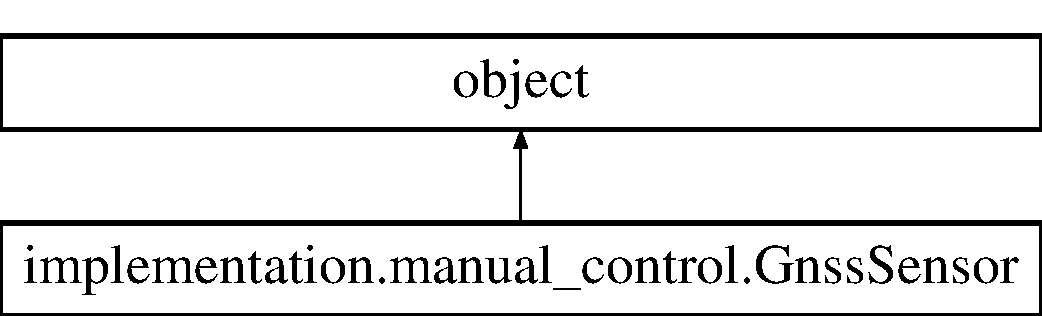
\includegraphics[height=2.000000cm]{classimplementation_1_1manual__control_1_1_gnss_sensor}
\end{center}
\end{figure}
\doxysubsection*{Public Member Functions}
\begin{DoxyCompactItemize}
\item 
def \mbox{\hyperlink{classimplementation_1_1manual__control_1_1_gnss_sensor_a5b79d29ae0f05aae01ed872f3d3ca156}{\+\_\+\+\_\+init\+\_\+\+\_\+}} (self, parent\+\_\+actor)
\end{DoxyCompactItemize}
\doxysubsection*{Public Attributes}
\begin{DoxyCompactItemize}
\item 
\mbox{\hyperlink{classimplementation_1_1manual__control_1_1_gnss_sensor_a55c8133724d2eb8b349a3c5fbf29f3ac}{sensor}}
\item 
\mbox{\hyperlink{classimplementation_1_1manual__control_1_1_gnss_sensor_a6b47354939272b7f92fcc80444866cf4}{lat}}
\item 
\mbox{\hyperlink{classimplementation_1_1manual__control_1_1_gnss_sensor_aff72b8285bcadf60c4aa0070359ec607}{lon}}
\end{DoxyCompactItemize}


\doxysubsection{Constructor \& Destructor Documentation}
\mbox{\Hypertarget{classimplementation_1_1manual__control_1_1_gnss_sensor_a5b79d29ae0f05aae01ed872f3d3ca156}\label{classimplementation_1_1manual__control_1_1_gnss_sensor_a5b79d29ae0f05aae01ed872f3d3ca156}} 
\index{implementation.manual\_control.GnssSensor@{implementation.manual\_control.GnssSensor}!\_\_init\_\_@{\_\_init\_\_}}
\index{\_\_init\_\_@{\_\_init\_\_}!implementation.manual\_control.GnssSensor@{implementation.manual\_control.GnssSensor}}
\doxysubsubsection{\texorpdfstring{\_\_init\_\_()}{\_\_init\_\_()}}
{\footnotesize\ttfamily def implementation.\+manual\+\_\+control.\+Gnss\+Sensor.\+\_\+\+\_\+init\+\_\+\+\_\+ (\begin{DoxyParamCaption}\item[{}]{self,  }\item[{}]{parent\+\_\+actor }\end{DoxyParamCaption})}



\doxysubsection{Member Data Documentation}
\mbox{\Hypertarget{classimplementation_1_1manual__control_1_1_gnss_sensor_a6b47354939272b7f92fcc80444866cf4}\label{classimplementation_1_1manual__control_1_1_gnss_sensor_a6b47354939272b7f92fcc80444866cf4}} 
\index{implementation.manual\_control.GnssSensor@{implementation.manual\_control.GnssSensor}!lat@{lat}}
\index{lat@{lat}!implementation.manual\_control.GnssSensor@{implementation.manual\_control.GnssSensor}}
\doxysubsubsection{\texorpdfstring{lat}{lat}}
{\footnotesize\ttfamily implementation.\+manual\+\_\+control.\+Gnss\+Sensor.\+lat}

\mbox{\Hypertarget{classimplementation_1_1manual__control_1_1_gnss_sensor_aff72b8285bcadf60c4aa0070359ec607}\label{classimplementation_1_1manual__control_1_1_gnss_sensor_aff72b8285bcadf60c4aa0070359ec607}} 
\index{implementation.manual\_control.GnssSensor@{implementation.manual\_control.GnssSensor}!lon@{lon}}
\index{lon@{lon}!implementation.manual\_control.GnssSensor@{implementation.manual\_control.GnssSensor}}
\doxysubsubsection{\texorpdfstring{lon}{lon}}
{\footnotesize\ttfamily implementation.\+manual\+\_\+control.\+Gnss\+Sensor.\+lon}

\mbox{\Hypertarget{classimplementation_1_1manual__control_1_1_gnss_sensor_a55c8133724d2eb8b349a3c5fbf29f3ac}\label{classimplementation_1_1manual__control_1_1_gnss_sensor_a55c8133724d2eb8b349a3c5fbf29f3ac}} 
\index{implementation.manual\_control.GnssSensor@{implementation.manual\_control.GnssSensor}!sensor@{sensor}}
\index{sensor@{sensor}!implementation.manual\_control.GnssSensor@{implementation.manual\_control.GnssSensor}}
\doxysubsubsection{\texorpdfstring{sensor}{sensor}}
{\footnotesize\ttfamily implementation.\+manual\+\_\+control.\+Gnss\+Sensor.\+sensor}



The documentation for this class was generated from the following file\+:\begin{DoxyCompactItemize}
\item 
implementation/\mbox{\hyperlink{manual__control_8py}{manual\+\_\+control.\+py}}\end{DoxyCompactItemize}

\hypertarget{classimplementation_1_1manual__control_1_1_help_text}{}\section{implementation.\+manual\+\_\+control.\+Help\+Text Class Reference}
\label{classimplementation_1_1manual__control_1_1_help_text}\index{implementation.\+manual\+\_\+control.\+Help\+Text@{implementation.\+manual\+\_\+control.\+Help\+Text}}
Inheritance diagram for implementation.\+manual\+\_\+control.\+Help\+Text\+:\begin{figure}[H]
\begin{center}
\leavevmode
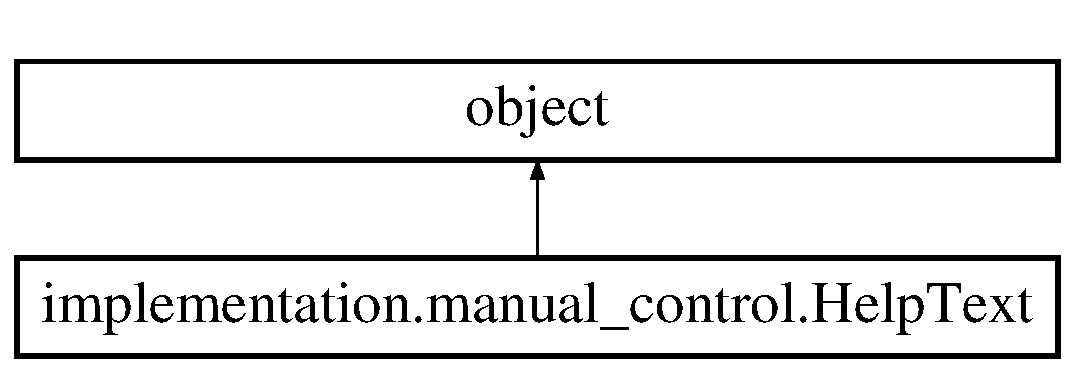
\includegraphics[height=2.000000cm]{classimplementation_1_1manual__control_1_1_help_text}
\end{center}
\end{figure}
\subsection*{Public Member Functions}
\begin{DoxyCompactItemize}
\item 
def \hyperlink{classimplementation_1_1manual__control_1_1_help_text_a44a93d3a97a10f0bff24b87d9801df22}{\+\_\+\+\_\+init\+\_\+\+\_\+} (self, \hyperlink{classimplementation_1_1manual__control_1_1_help_text_af4a0194dd1d3b501def507f74fb34c66}{font}, width, height)
\item 
def \hyperlink{classimplementation_1_1manual__control_1_1_help_text_a6e4eebd3ea87100d4176bcfacd5d4dc3}{toggle} (self)
\item 
def \hyperlink{classimplementation_1_1manual__control_1_1_help_text_a85830f8209380e27dde8bdc6f31c2606}{render} (self, display)
\end{DoxyCompactItemize}
\subsection*{Public Attributes}
\begin{DoxyCompactItemize}
\item 
\hyperlink{classimplementation_1_1manual__control_1_1_help_text_af4a0194dd1d3b501def507f74fb34c66}{font}
\item 
\hyperlink{classimplementation_1_1manual__control_1_1_help_text_a8953802c95907a76b33501087559f89f}{line\+\_\+space}
\item 
\hyperlink{classimplementation_1_1manual__control_1_1_help_text_ab709d6b17dccf7aa8d72baa89521e5ec}{dim}
\item 
\hyperlink{classimplementation_1_1manual__control_1_1_help_text_a48a3e7d984f55e2ebdb887dad75c06ff}{pos}
\item 
\hyperlink{classimplementation_1_1manual__control_1_1_help_text_a1f58691166a9446ef4e969868806cb7f}{seconds\+\_\+left}
\item 
\hyperlink{classimplementation_1_1manual__control_1_1_help_text_af392ae943c1d955198cbf6f4b6da3f8e}{surface}
\end{DoxyCompactItemize}


\subsection{Detailed Description}
\begin{DoxyVerb}Helper class to handle text output using pygame\end{DoxyVerb}
 

\subsection{Constructor \& Destructor Documentation}
\mbox{\Hypertarget{classimplementation_1_1manual__control_1_1_help_text_a44a93d3a97a10f0bff24b87d9801df22}\label{classimplementation_1_1manual__control_1_1_help_text_a44a93d3a97a10f0bff24b87d9801df22}} 
\index{implementation\+::manual\+\_\+control\+::\+Help\+Text@{implementation\+::manual\+\_\+control\+::\+Help\+Text}!\+\_\+\+\_\+init\+\_\+\+\_\+@{\+\_\+\+\_\+init\+\_\+\+\_\+}}
\index{\+\_\+\+\_\+init\+\_\+\+\_\+@{\+\_\+\+\_\+init\+\_\+\+\_\+}!implementation\+::manual\+\_\+control\+::\+Help\+Text@{implementation\+::manual\+\_\+control\+::\+Help\+Text}}
\subsubsection{\texorpdfstring{\+\_\+\+\_\+init\+\_\+\+\_\+()}{\_\_init\_\_()}}
{\footnotesize\ttfamily def implementation.\+manual\+\_\+control.\+Help\+Text.\+\_\+\+\_\+init\+\_\+\+\_\+ (\begin{DoxyParamCaption}\item[{}]{self,  }\item[{}]{font,  }\item[{}]{width,  }\item[{}]{height }\end{DoxyParamCaption})}



\subsection{Member Function Documentation}
\mbox{\Hypertarget{classimplementation_1_1manual__control_1_1_help_text_a85830f8209380e27dde8bdc6f31c2606}\label{classimplementation_1_1manual__control_1_1_help_text_a85830f8209380e27dde8bdc6f31c2606}} 
\index{implementation\+::manual\+\_\+control\+::\+Help\+Text@{implementation\+::manual\+\_\+control\+::\+Help\+Text}!render@{render}}
\index{render@{render}!implementation\+::manual\+\_\+control\+::\+Help\+Text@{implementation\+::manual\+\_\+control\+::\+Help\+Text}}
\subsubsection{\texorpdfstring{render()}{render()}}
{\footnotesize\ttfamily def implementation.\+manual\+\_\+control.\+Help\+Text.\+render (\begin{DoxyParamCaption}\item[{}]{self,  }\item[{}]{display }\end{DoxyParamCaption})}

\mbox{\Hypertarget{classimplementation_1_1manual__control_1_1_help_text_a6e4eebd3ea87100d4176bcfacd5d4dc3}\label{classimplementation_1_1manual__control_1_1_help_text_a6e4eebd3ea87100d4176bcfacd5d4dc3}} 
\index{implementation\+::manual\+\_\+control\+::\+Help\+Text@{implementation\+::manual\+\_\+control\+::\+Help\+Text}!toggle@{toggle}}
\index{toggle@{toggle}!implementation\+::manual\+\_\+control\+::\+Help\+Text@{implementation\+::manual\+\_\+control\+::\+Help\+Text}}
\subsubsection{\texorpdfstring{toggle()}{toggle()}}
{\footnotesize\ttfamily def implementation.\+manual\+\_\+control.\+Help\+Text.\+toggle (\begin{DoxyParamCaption}\item[{}]{self }\end{DoxyParamCaption})}



\subsection{Member Data Documentation}
\mbox{\Hypertarget{classimplementation_1_1manual__control_1_1_help_text_ab709d6b17dccf7aa8d72baa89521e5ec}\label{classimplementation_1_1manual__control_1_1_help_text_ab709d6b17dccf7aa8d72baa89521e5ec}} 
\index{implementation\+::manual\+\_\+control\+::\+Help\+Text@{implementation\+::manual\+\_\+control\+::\+Help\+Text}!dim@{dim}}
\index{dim@{dim}!implementation\+::manual\+\_\+control\+::\+Help\+Text@{implementation\+::manual\+\_\+control\+::\+Help\+Text}}
\subsubsection{\texorpdfstring{dim}{dim}}
{\footnotesize\ttfamily implementation.\+manual\+\_\+control.\+Help\+Text.\+dim}

\mbox{\Hypertarget{classimplementation_1_1manual__control_1_1_help_text_af4a0194dd1d3b501def507f74fb34c66}\label{classimplementation_1_1manual__control_1_1_help_text_af4a0194dd1d3b501def507f74fb34c66}} 
\index{implementation\+::manual\+\_\+control\+::\+Help\+Text@{implementation\+::manual\+\_\+control\+::\+Help\+Text}!font@{font}}
\index{font@{font}!implementation\+::manual\+\_\+control\+::\+Help\+Text@{implementation\+::manual\+\_\+control\+::\+Help\+Text}}
\subsubsection{\texorpdfstring{font}{font}}
{\footnotesize\ttfamily implementation.\+manual\+\_\+control.\+Help\+Text.\+font}

\mbox{\Hypertarget{classimplementation_1_1manual__control_1_1_help_text_a8953802c95907a76b33501087559f89f}\label{classimplementation_1_1manual__control_1_1_help_text_a8953802c95907a76b33501087559f89f}} 
\index{implementation\+::manual\+\_\+control\+::\+Help\+Text@{implementation\+::manual\+\_\+control\+::\+Help\+Text}!line\+\_\+space@{line\+\_\+space}}
\index{line\+\_\+space@{line\+\_\+space}!implementation\+::manual\+\_\+control\+::\+Help\+Text@{implementation\+::manual\+\_\+control\+::\+Help\+Text}}
\subsubsection{\texorpdfstring{line\+\_\+space}{line\_space}}
{\footnotesize\ttfamily implementation.\+manual\+\_\+control.\+Help\+Text.\+line\+\_\+space}

\mbox{\Hypertarget{classimplementation_1_1manual__control_1_1_help_text_a48a3e7d984f55e2ebdb887dad75c06ff}\label{classimplementation_1_1manual__control_1_1_help_text_a48a3e7d984f55e2ebdb887dad75c06ff}} 
\index{implementation\+::manual\+\_\+control\+::\+Help\+Text@{implementation\+::manual\+\_\+control\+::\+Help\+Text}!pos@{pos}}
\index{pos@{pos}!implementation\+::manual\+\_\+control\+::\+Help\+Text@{implementation\+::manual\+\_\+control\+::\+Help\+Text}}
\subsubsection{\texorpdfstring{pos}{pos}}
{\footnotesize\ttfamily implementation.\+manual\+\_\+control.\+Help\+Text.\+pos}

\mbox{\Hypertarget{classimplementation_1_1manual__control_1_1_help_text_a1f58691166a9446ef4e969868806cb7f}\label{classimplementation_1_1manual__control_1_1_help_text_a1f58691166a9446ef4e969868806cb7f}} 
\index{implementation\+::manual\+\_\+control\+::\+Help\+Text@{implementation\+::manual\+\_\+control\+::\+Help\+Text}!seconds\+\_\+left@{seconds\+\_\+left}}
\index{seconds\+\_\+left@{seconds\+\_\+left}!implementation\+::manual\+\_\+control\+::\+Help\+Text@{implementation\+::manual\+\_\+control\+::\+Help\+Text}}
\subsubsection{\texorpdfstring{seconds\+\_\+left}{seconds\_left}}
{\footnotesize\ttfamily implementation.\+manual\+\_\+control.\+Help\+Text.\+seconds\+\_\+left}

\mbox{\Hypertarget{classimplementation_1_1manual__control_1_1_help_text_af392ae943c1d955198cbf6f4b6da3f8e}\label{classimplementation_1_1manual__control_1_1_help_text_af392ae943c1d955198cbf6f4b6da3f8e}} 
\index{implementation\+::manual\+\_\+control\+::\+Help\+Text@{implementation\+::manual\+\_\+control\+::\+Help\+Text}!surface@{surface}}
\index{surface@{surface}!implementation\+::manual\+\_\+control\+::\+Help\+Text@{implementation\+::manual\+\_\+control\+::\+Help\+Text}}
\subsubsection{\texorpdfstring{surface}{surface}}
{\footnotesize\ttfamily implementation.\+manual\+\_\+control.\+Help\+Text.\+surface}



The documentation for this class was generated from the following file\+:\begin{DoxyCompactItemize}
\item 
implementation/\hyperlink{manual__control_8py}{manual\+\_\+control.\+py}\end{DoxyCompactItemize}

\hypertarget{classimplementation_1_1manual__control_1_1_h_u_d}{}\doxysection{implementation.\+manual\+\_\+control.\+H\+UD Class Reference}
\label{classimplementation_1_1manual__control_1_1_h_u_d}\index{implementation.manual\_control.HUD@{implementation.manual\_control.HUD}}
Inheritance diagram for implementation.\+manual\+\_\+control.\+H\+UD\+:\begin{figure}[H]
\begin{center}
\leavevmode
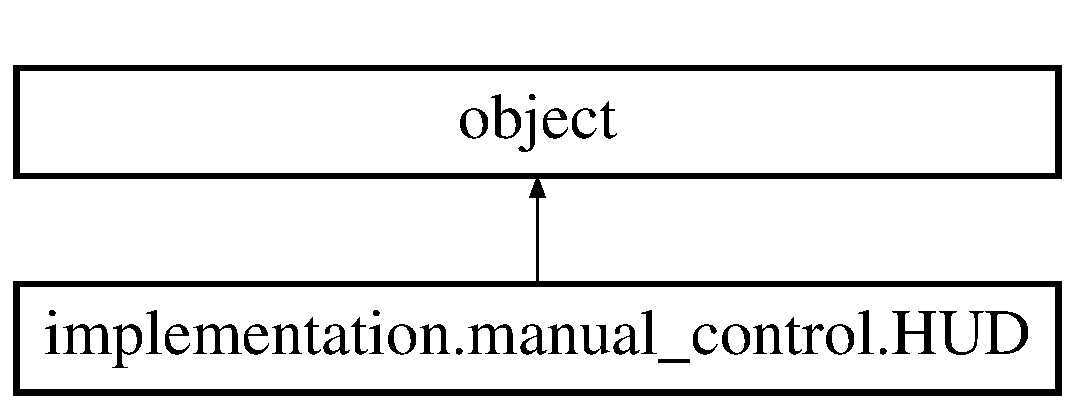
\includegraphics[height=2.000000cm]{classimplementation_1_1manual__control_1_1_h_u_d}
\end{center}
\end{figure}
\doxysubsection*{Public Member Functions}
\begin{DoxyCompactItemize}
\item 
def \mbox{\hyperlink{classimplementation_1_1manual__control_1_1_h_u_d_a0cfbc7b3d4bd4442e0ded8bb75d5cc93}{\+\_\+\+\_\+init\+\_\+\+\_\+}} (self, width, height)
\item 
def \mbox{\hyperlink{classimplementation_1_1manual__control_1_1_h_u_d_a47c1ee42156cddbb581135dcd38c13a0}{on\+\_\+world\+\_\+tick}} (self, timestamp)
\item 
def \mbox{\hyperlink{classimplementation_1_1manual__control_1_1_h_u_d_a07f4da3ec0a20a6f90fcf9c7a34791b4}{tick}} (self, world, clock)
\item 
def \mbox{\hyperlink{classimplementation_1_1manual__control_1_1_h_u_d_a68d0dce74e4dbdd46737fd6b202df6e2}{toggle\+\_\+info}} (self)
\item 
def \mbox{\hyperlink{classimplementation_1_1manual__control_1_1_h_u_d_ab7dc7fd919aed4a08ae3051964fc823d}{notification}} (self, text, seconds=2.\+0)
\item 
def \mbox{\hyperlink{classimplementation_1_1manual__control_1_1_h_u_d_a54880fbc86435b853cf91cd551db8f52}{error}} (self, text)
\item 
def \mbox{\hyperlink{classimplementation_1_1manual__control_1_1_h_u_d_a8fbc629658fa677fd78f966648e5f1b5}{render}} (self, display)
\end{DoxyCompactItemize}
\doxysubsection*{Public Attributes}
\begin{DoxyCompactItemize}
\item 
\mbox{\hyperlink{classimplementation_1_1manual__control_1_1_h_u_d_a4eec82f55878222edf93d0742dcd133e}{dim}}
\item 
\mbox{\hyperlink{classimplementation_1_1manual__control_1_1_h_u_d_aea7f44c49123f8f4d38ba12fe15332dc}{help}}
\item 
\mbox{\hyperlink{classimplementation_1_1manual__control_1_1_h_u_d_a418909515eb46abea3fcb26f42020c68}{server\+\_\+fps}}
\item 
\mbox{\hyperlink{classimplementation_1_1manual__control_1_1_h_u_d_a83d58bd2583209bd349cfcd22e40784c}{frame}}
\item 
\mbox{\hyperlink{classimplementation_1_1manual__control_1_1_h_u_d_a9030c299b81352e1cea2e1f3eb8498d8}{simulation\+\_\+time}}
\end{DoxyCompactItemize}


\doxysubsection{Constructor \& Destructor Documentation}
\mbox{\Hypertarget{classimplementation_1_1manual__control_1_1_h_u_d_a0cfbc7b3d4bd4442e0ded8bb75d5cc93}\label{classimplementation_1_1manual__control_1_1_h_u_d_a0cfbc7b3d4bd4442e0ded8bb75d5cc93}} 
\index{implementation.manual\_control.HUD@{implementation.manual\_control.HUD}!\_\_init\_\_@{\_\_init\_\_}}
\index{\_\_init\_\_@{\_\_init\_\_}!implementation.manual\_control.HUD@{implementation.manual\_control.HUD}}
\doxysubsubsection{\texorpdfstring{\_\_init\_\_()}{\_\_init\_\_()}}
{\footnotesize\ttfamily def implementation.\+manual\+\_\+control.\+H\+U\+D.\+\_\+\+\_\+init\+\_\+\+\_\+ (\begin{DoxyParamCaption}\item[{}]{self,  }\item[{}]{width,  }\item[{}]{height }\end{DoxyParamCaption})}



\doxysubsection{Member Function Documentation}
\mbox{\Hypertarget{classimplementation_1_1manual__control_1_1_h_u_d_a54880fbc86435b853cf91cd551db8f52}\label{classimplementation_1_1manual__control_1_1_h_u_d_a54880fbc86435b853cf91cd551db8f52}} 
\index{implementation.manual\_control.HUD@{implementation.manual\_control.HUD}!error@{error}}
\index{error@{error}!implementation.manual\_control.HUD@{implementation.manual\_control.HUD}}
\doxysubsubsection{\texorpdfstring{error()}{error()}}
{\footnotesize\ttfamily def implementation.\+manual\+\_\+control.\+H\+U\+D.\+error (\begin{DoxyParamCaption}\item[{}]{self,  }\item[{}]{text }\end{DoxyParamCaption})}

\mbox{\Hypertarget{classimplementation_1_1manual__control_1_1_h_u_d_ab7dc7fd919aed4a08ae3051964fc823d}\label{classimplementation_1_1manual__control_1_1_h_u_d_ab7dc7fd919aed4a08ae3051964fc823d}} 
\index{implementation.manual\_control.HUD@{implementation.manual\_control.HUD}!notification@{notification}}
\index{notification@{notification}!implementation.manual\_control.HUD@{implementation.manual\_control.HUD}}
\doxysubsubsection{\texorpdfstring{notification()}{notification()}}
{\footnotesize\ttfamily def implementation.\+manual\+\_\+control.\+H\+U\+D.\+notification (\begin{DoxyParamCaption}\item[{}]{self,  }\item[{}]{text,  }\item[{}]{seconds = {\ttfamily 2.0} }\end{DoxyParamCaption})}

\mbox{\Hypertarget{classimplementation_1_1manual__control_1_1_h_u_d_a47c1ee42156cddbb581135dcd38c13a0}\label{classimplementation_1_1manual__control_1_1_h_u_d_a47c1ee42156cddbb581135dcd38c13a0}} 
\index{implementation.manual\_control.HUD@{implementation.manual\_control.HUD}!on\_world\_tick@{on\_world\_tick}}
\index{on\_world\_tick@{on\_world\_tick}!implementation.manual\_control.HUD@{implementation.manual\_control.HUD}}
\doxysubsubsection{\texorpdfstring{on\_world\_tick()}{on\_world\_tick()}}
{\footnotesize\ttfamily def implementation.\+manual\+\_\+control.\+H\+U\+D.\+on\+\_\+world\+\_\+tick (\begin{DoxyParamCaption}\item[{}]{self,  }\item[{}]{timestamp }\end{DoxyParamCaption})}

\mbox{\Hypertarget{classimplementation_1_1manual__control_1_1_h_u_d_a8fbc629658fa677fd78f966648e5f1b5}\label{classimplementation_1_1manual__control_1_1_h_u_d_a8fbc629658fa677fd78f966648e5f1b5}} 
\index{implementation.manual\_control.HUD@{implementation.manual\_control.HUD}!render@{render}}
\index{render@{render}!implementation.manual\_control.HUD@{implementation.manual\_control.HUD}}
\doxysubsubsection{\texorpdfstring{render()}{render()}}
{\footnotesize\ttfamily def implementation.\+manual\+\_\+control.\+H\+U\+D.\+render (\begin{DoxyParamCaption}\item[{}]{self,  }\item[{}]{display }\end{DoxyParamCaption})}

\mbox{\Hypertarget{classimplementation_1_1manual__control_1_1_h_u_d_a07f4da3ec0a20a6f90fcf9c7a34791b4}\label{classimplementation_1_1manual__control_1_1_h_u_d_a07f4da3ec0a20a6f90fcf9c7a34791b4}} 
\index{implementation.manual\_control.HUD@{implementation.manual\_control.HUD}!tick@{tick}}
\index{tick@{tick}!implementation.manual\_control.HUD@{implementation.manual\_control.HUD}}
\doxysubsubsection{\texorpdfstring{tick()}{tick()}}
{\footnotesize\ttfamily def implementation.\+manual\+\_\+control.\+H\+U\+D.\+tick (\begin{DoxyParamCaption}\item[{}]{self,  }\item[{}]{world,  }\item[{}]{clock }\end{DoxyParamCaption})}

\mbox{\Hypertarget{classimplementation_1_1manual__control_1_1_h_u_d_a68d0dce74e4dbdd46737fd6b202df6e2}\label{classimplementation_1_1manual__control_1_1_h_u_d_a68d0dce74e4dbdd46737fd6b202df6e2}} 
\index{implementation.manual\_control.HUD@{implementation.manual\_control.HUD}!toggle\_info@{toggle\_info}}
\index{toggle\_info@{toggle\_info}!implementation.manual\_control.HUD@{implementation.manual\_control.HUD}}
\doxysubsubsection{\texorpdfstring{toggle\_info()}{toggle\_info()}}
{\footnotesize\ttfamily def implementation.\+manual\+\_\+control.\+H\+U\+D.\+toggle\+\_\+info (\begin{DoxyParamCaption}\item[{}]{self }\end{DoxyParamCaption})}



\doxysubsection{Member Data Documentation}
\mbox{\Hypertarget{classimplementation_1_1manual__control_1_1_h_u_d_a4eec82f55878222edf93d0742dcd133e}\label{classimplementation_1_1manual__control_1_1_h_u_d_a4eec82f55878222edf93d0742dcd133e}} 
\index{implementation.manual\_control.HUD@{implementation.manual\_control.HUD}!dim@{dim}}
\index{dim@{dim}!implementation.manual\_control.HUD@{implementation.manual\_control.HUD}}
\doxysubsubsection{\texorpdfstring{dim}{dim}}
{\footnotesize\ttfamily implementation.\+manual\+\_\+control.\+H\+U\+D.\+dim}

\mbox{\Hypertarget{classimplementation_1_1manual__control_1_1_h_u_d_a83d58bd2583209bd349cfcd22e40784c}\label{classimplementation_1_1manual__control_1_1_h_u_d_a83d58bd2583209bd349cfcd22e40784c}} 
\index{implementation.manual\_control.HUD@{implementation.manual\_control.HUD}!frame@{frame}}
\index{frame@{frame}!implementation.manual\_control.HUD@{implementation.manual\_control.HUD}}
\doxysubsubsection{\texorpdfstring{frame}{frame}}
{\footnotesize\ttfamily implementation.\+manual\+\_\+control.\+H\+U\+D.\+frame}

\mbox{\Hypertarget{classimplementation_1_1manual__control_1_1_h_u_d_aea7f44c49123f8f4d38ba12fe15332dc}\label{classimplementation_1_1manual__control_1_1_h_u_d_aea7f44c49123f8f4d38ba12fe15332dc}} 
\index{implementation.manual\_control.HUD@{implementation.manual\_control.HUD}!help@{help}}
\index{help@{help}!implementation.manual\_control.HUD@{implementation.manual\_control.HUD}}
\doxysubsubsection{\texorpdfstring{help}{help}}
{\footnotesize\ttfamily implementation.\+manual\+\_\+control.\+H\+U\+D.\+help}

\mbox{\Hypertarget{classimplementation_1_1manual__control_1_1_h_u_d_a418909515eb46abea3fcb26f42020c68}\label{classimplementation_1_1manual__control_1_1_h_u_d_a418909515eb46abea3fcb26f42020c68}} 
\index{implementation.manual\_control.HUD@{implementation.manual\_control.HUD}!server\_fps@{server\_fps}}
\index{server\_fps@{server\_fps}!implementation.manual\_control.HUD@{implementation.manual\_control.HUD}}
\doxysubsubsection{\texorpdfstring{server\_fps}{server\_fps}}
{\footnotesize\ttfamily implementation.\+manual\+\_\+control.\+H\+U\+D.\+server\+\_\+fps}

\mbox{\Hypertarget{classimplementation_1_1manual__control_1_1_h_u_d_a9030c299b81352e1cea2e1f3eb8498d8}\label{classimplementation_1_1manual__control_1_1_h_u_d_a9030c299b81352e1cea2e1f3eb8498d8}} 
\index{implementation.manual\_control.HUD@{implementation.manual\_control.HUD}!simulation\_time@{simulation\_time}}
\index{simulation\_time@{simulation\_time}!implementation.manual\_control.HUD@{implementation.manual\_control.HUD}}
\doxysubsubsection{\texorpdfstring{simulation\_time}{simulation\_time}}
{\footnotesize\ttfamily implementation.\+manual\+\_\+control.\+H\+U\+D.\+simulation\+\_\+time}



The documentation for this class was generated from the following file\+:\begin{DoxyCompactItemize}
\item 
implementation/\mbox{\hyperlink{manual__control_8py}{manual\+\_\+control.\+py}}\end{DoxyCompactItemize}

\hypertarget{classimplementation_1_1manual__control_1_1_i_m_u_sensor}{}\doxysection{implementation.\+manual\+\_\+control.\+I\+M\+U\+Sensor Class Reference}
\label{classimplementation_1_1manual__control_1_1_i_m_u_sensor}\index{implementation.manual\_control.IMUSensor@{implementation.manual\_control.IMUSensor}}
Inheritance diagram for implementation.\+manual\+\_\+control.\+I\+M\+U\+Sensor\+:\begin{figure}[H]
\begin{center}
\leavevmode
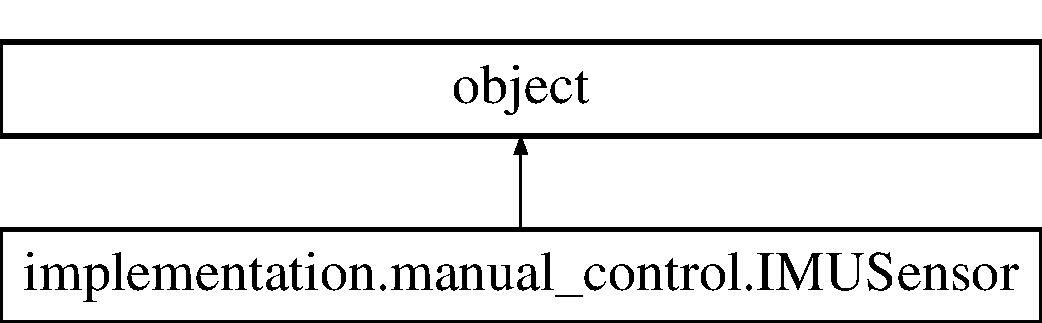
\includegraphics[height=2.000000cm]{classimplementation_1_1manual__control_1_1_i_m_u_sensor}
\end{center}
\end{figure}
\doxysubsection*{Public Member Functions}
\begin{DoxyCompactItemize}
\item 
def \mbox{\hyperlink{classimplementation_1_1manual__control_1_1_i_m_u_sensor_a08519b07c706defc81db7bf62887534d}{\+\_\+\+\_\+init\+\_\+\+\_\+}} (self, parent\+\_\+actor)
\end{DoxyCompactItemize}
\doxysubsection*{Public Attributes}
\begin{DoxyCompactItemize}
\item 
\mbox{\hyperlink{classimplementation_1_1manual__control_1_1_i_m_u_sensor_a0c0695278644bcb85488a371a6e5658c}{sensor}}
\item 
\mbox{\hyperlink{classimplementation_1_1manual__control_1_1_i_m_u_sensor_a578bd537303fe8a99c4047982519ea45}{accelerometer}}
\item 
\mbox{\hyperlink{classimplementation_1_1manual__control_1_1_i_m_u_sensor_a9f9e117d6935ed897d8ab058112adb90}{gyroscope}}
\item 
\mbox{\hyperlink{classimplementation_1_1manual__control_1_1_i_m_u_sensor_ac822546a1d64677ffcd5ceeb9b4033d5}{compass}}
\end{DoxyCompactItemize}


\doxysubsection{Constructor \& Destructor Documentation}
\mbox{\Hypertarget{classimplementation_1_1manual__control_1_1_i_m_u_sensor_a08519b07c706defc81db7bf62887534d}\label{classimplementation_1_1manual__control_1_1_i_m_u_sensor_a08519b07c706defc81db7bf62887534d}} 
\index{implementation.manual\_control.IMUSensor@{implementation.manual\_control.IMUSensor}!\_\_init\_\_@{\_\_init\_\_}}
\index{\_\_init\_\_@{\_\_init\_\_}!implementation.manual\_control.IMUSensor@{implementation.manual\_control.IMUSensor}}
\doxysubsubsection{\texorpdfstring{\_\_init\_\_()}{\_\_init\_\_()}}
{\footnotesize\ttfamily def implementation.\+manual\+\_\+control.\+I\+M\+U\+Sensor.\+\_\+\+\_\+init\+\_\+\+\_\+ (\begin{DoxyParamCaption}\item[{}]{self,  }\item[{}]{parent\+\_\+actor }\end{DoxyParamCaption})}



\doxysubsection{Member Data Documentation}
\mbox{\Hypertarget{classimplementation_1_1manual__control_1_1_i_m_u_sensor_a578bd537303fe8a99c4047982519ea45}\label{classimplementation_1_1manual__control_1_1_i_m_u_sensor_a578bd537303fe8a99c4047982519ea45}} 
\index{implementation.manual\_control.IMUSensor@{implementation.manual\_control.IMUSensor}!accelerometer@{accelerometer}}
\index{accelerometer@{accelerometer}!implementation.manual\_control.IMUSensor@{implementation.manual\_control.IMUSensor}}
\doxysubsubsection{\texorpdfstring{accelerometer}{accelerometer}}
{\footnotesize\ttfamily implementation.\+manual\+\_\+control.\+I\+M\+U\+Sensor.\+accelerometer}

\mbox{\Hypertarget{classimplementation_1_1manual__control_1_1_i_m_u_sensor_ac822546a1d64677ffcd5ceeb9b4033d5}\label{classimplementation_1_1manual__control_1_1_i_m_u_sensor_ac822546a1d64677ffcd5ceeb9b4033d5}} 
\index{implementation.manual\_control.IMUSensor@{implementation.manual\_control.IMUSensor}!compass@{compass}}
\index{compass@{compass}!implementation.manual\_control.IMUSensor@{implementation.manual\_control.IMUSensor}}
\doxysubsubsection{\texorpdfstring{compass}{compass}}
{\footnotesize\ttfamily implementation.\+manual\+\_\+control.\+I\+M\+U\+Sensor.\+compass}

\mbox{\Hypertarget{classimplementation_1_1manual__control_1_1_i_m_u_sensor_a9f9e117d6935ed897d8ab058112adb90}\label{classimplementation_1_1manual__control_1_1_i_m_u_sensor_a9f9e117d6935ed897d8ab058112adb90}} 
\index{implementation.manual\_control.IMUSensor@{implementation.manual\_control.IMUSensor}!gyroscope@{gyroscope}}
\index{gyroscope@{gyroscope}!implementation.manual\_control.IMUSensor@{implementation.manual\_control.IMUSensor}}
\doxysubsubsection{\texorpdfstring{gyroscope}{gyroscope}}
{\footnotesize\ttfamily implementation.\+manual\+\_\+control.\+I\+M\+U\+Sensor.\+gyroscope}

\mbox{\Hypertarget{classimplementation_1_1manual__control_1_1_i_m_u_sensor_a0c0695278644bcb85488a371a6e5658c}\label{classimplementation_1_1manual__control_1_1_i_m_u_sensor_a0c0695278644bcb85488a371a6e5658c}} 
\index{implementation.manual\_control.IMUSensor@{implementation.manual\_control.IMUSensor}!sensor@{sensor}}
\index{sensor@{sensor}!implementation.manual\_control.IMUSensor@{implementation.manual\_control.IMUSensor}}
\doxysubsubsection{\texorpdfstring{sensor}{sensor}}
{\footnotesize\ttfamily implementation.\+manual\+\_\+control.\+I\+M\+U\+Sensor.\+sensor}



The documentation for this class was generated from the following file\+:\begin{DoxyCompactItemize}
\item 
implementation/\mbox{\hyperlink{manual__control_8py}{manual\+\_\+control.\+py}}\end{DoxyCompactItemize}

\hypertarget{classimplementation_1_1data__model_1_1positions_1_1_in_route_position}{}\section{implementation.\+data\+\_\+model.\+positions.\+In\+Route\+Position Class Reference}
\label{classimplementation_1_1data__model_1_1positions_1_1_in_route_position}\index{implementation.\+data\+\_\+model.\+positions.\+In\+Route\+Position@{implementation.\+data\+\_\+model.\+positions.\+In\+Route\+Position}}
\subsection*{Static Public Attributes}
\begin{DoxyCompactItemize}
\item 
\hyperlink{classimplementation_1_1data__model_1_1positions_1_1_in_route_position_a1ae2ad89868f70da9497da872c849bd9}{Position\+Of\+Current\+Entity}
\item 
\hyperlink{classimplementation_1_1data__model_1_1positions_1_1_in_route_position_a2bb8fcf429c82f6601615c3480400827}{Position\+In\+Road\+Coordinates}
\item 
\hyperlink{classimplementation_1_1data__model_1_1positions_1_1_in_route_position_a113f40938b26b069ebf13ea23fdc3338}{Position\+In\+Lane\+Coordinates}
\end{DoxyCompactItemize}


\subsection{Member Data Documentation}
\mbox{\Hypertarget{classimplementation_1_1data__model_1_1positions_1_1_in_route_position_a113f40938b26b069ebf13ea23fdc3338}\label{classimplementation_1_1data__model_1_1positions_1_1_in_route_position_a113f40938b26b069ebf13ea23fdc3338}} 
\index{implementation\+::data\+\_\+model\+::positions\+::\+In\+Route\+Position@{implementation\+::data\+\_\+model\+::positions\+::\+In\+Route\+Position}!Position\+In\+Lane\+Coordinates@{Position\+In\+Lane\+Coordinates}}
\index{Position\+In\+Lane\+Coordinates@{Position\+In\+Lane\+Coordinates}!implementation\+::data\+\_\+model\+::positions\+::\+In\+Route\+Position@{implementation\+::data\+\_\+model\+::positions\+::\+In\+Route\+Position}}
\subsubsection{\texorpdfstring{Position\+In\+Lane\+Coordinates}{PositionInLaneCoordinates}}
{\footnotesize\ttfamily implementation.\+data\+\_\+model.\+positions.\+In\+Route\+Position.\+Position\+In\+Lane\+Coordinates\hspace{0.3cm}{\ttfamily [static]}}

\mbox{\Hypertarget{classimplementation_1_1data__model_1_1positions_1_1_in_route_position_a2bb8fcf429c82f6601615c3480400827}\label{classimplementation_1_1data__model_1_1positions_1_1_in_route_position_a2bb8fcf429c82f6601615c3480400827}} 
\index{implementation\+::data\+\_\+model\+::positions\+::\+In\+Route\+Position@{implementation\+::data\+\_\+model\+::positions\+::\+In\+Route\+Position}!Position\+In\+Road\+Coordinates@{Position\+In\+Road\+Coordinates}}
\index{Position\+In\+Road\+Coordinates@{Position\+In\+Road\+Coordinates}!implementation\+::data\+\_\+model\+::positions\+::\+In\+Route\+Position@{implementation\+::data\+\_\+model\+::positions\+::\+In\+Route\+Position}}
\subsubsection{\texorpdfstring{Position\+In\+Road\+Coordinates}{PositionInRoadCoordinates}}
{\footnotesize\ttfamily implementation.\+data\+\_\+model.\+positions.\+In\+Route\+Position.\+Position\+In\+Road\+Coordinates\hspace{0.3cm}{\ttfamily [static]}}

\mbox{\Hypertarget{classimplementation_1_1data__model_1_1positions_1_1_in_route_position_a1ae2ad89868f70da9497da872c849bd9}\label{classimplementation_1_1data__model_1_1positions_1_1_in_route_position_a1ae2ad89868f70da9497da872c849bd9}} 
\index{implementation\+::data\+\_\+model\+::positions\+::\+In\+Route\+Position@{implementation\+::data\+\_\+model\+::positions\+::\+In\+Route\+Position}!Position\+Of\+Current\+Entity@{Position\+Of\+Current\+Entity}}
\index{Position\+Of\+Current\+Entity@{Position\+Of\+Current\+Entity}!implementation\+::data\+\_\+model\+::positions\+::\+In\+Route\+Position@{implementation\+::data\+\_\+model\+::positions\+::\+In\+Route\+Position}}
\subsubsection{\texorpdfstring{Position\+Of\+Current\+Entity}{PositionOfCurrentEntity}}
{\footnotesize\ttfamily implementation.\+data\+\_\+model.\+positions.\+In\+Route\+Position.\+Position\+Of\+Current\+Entity\hspace{0.3cm}{\ttfamily [static]}}



The documentation for this class was generated from the following file\+:\begin{DoxyCompactItemize}
\item 
implementation/data\+\_\+model/\hyperlink{positions_8py}{positions.\+py}\end{DoxyCompactItemize}

\hypertarget{classimplementation_1_1manual__control_1_1_keyboard_control}{}\section{implementation.\+manual\+\_\+control.\+Keyboard\+Control Class Reference}
\label{classimplementation_1_1manual__control_1_1_keyboard_control}\index{implementation.\+manual\+\_\+control.\+Keyboard\+Control@{implementation.\+manual\+\_\+control.\+Keyboard\+Control}}
Inheritance diagram for implementation.\+manual\+\_\+control.\+Keyboard\+Control\+:\begin{figure}[H]
\begin{center}
\leavevmode
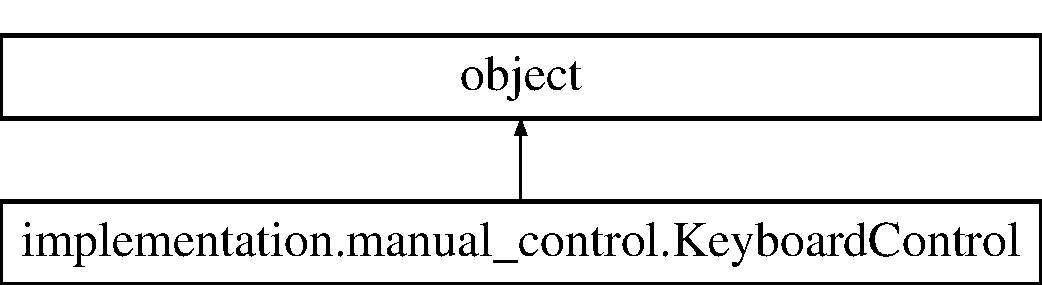
\includegraphics[height=2.000000cm]{classimplementation_1_1manual__control_1_1_keyboard_control}
\end{center}
\end{figure}
\subsection*{Public Member Functions}
\begin{DoxyCompactItemize}
\item 
def \hyperlink{classimplementation_1_1manual__control_1_1_keyboard_control_adeaf1dd5883f6ee4548ad8ee00ee9099}{\+\_\+\+\_\+init\+\_\+\+\_\+} (self, world, start\+\_\+in\+\_\+autopilot)
\item 
def \hyperlink{classimplementation_1_1manual__control_1_1_keyboard_control_a1217f115f0929922b01ba00a4aebf42c}{parse\+\_\+events} (self, client, world, clock)
\end{DoxyCompactItemize}


\subsection{Detailed Description}
\begin{DoxyVerb}Class that handles keyboard input.\end{DoxyVerb}
 

\subsection{Constructor \& Destructor Documentation}
\mbox{\Hypertarget{classimplementation_1_1manual__control_1_1_keyboard_control_adeaf1dd5883f6ee4548ad8ee00ee9099}\label{classimplementation_1_1manual__control_1_1_keyboard_control_adeaf1dd5883f6ee4548ad8ee00ee9099}} 
\index{implementation\+::manual\+\_\+control\+::\+Keyboard\+Control@{implementation\+::manual\+\_\+control\+::\+Keyboard\+Control}!\+\_\+\+\_\+init\+\_\+\+\_\+@{\+\_\+\+\_\+init\+\_\+\+\_\+}}
\index{\+\_\+\+\_\+init\+\_\+\+\_\+@{\+\_\+\+\_\+init\+\_\+\+\_\+}!implementation\+::manual\+\_\+control\+::\+Keyboard\+Control@{implementation\+::manual\+\_\+control\+::\+Keyboard\+Control}}
\subsubsection{\texorpdfstring{\+\_\+\+\_\+init\+\_\+\+\_\+()}{\_\_init\_\_()}}
{\footnotesize\ttfamily def implementation.\+manual\+\_\+control.\+Keyboard\+Control.\+\_\+\+\_\+init\+\_\+\+\_\+ (\begin{DoxyParamCaption}\item[{}]{self,  }\item[{}]{world,  }\item[{}]{start\+\_\+in\+\_\+autopilot }\end{DoxyParamCaption})}



\subsection{Member Function Documentation}
\mbox{\Hypertarget{classimplementation_1_1manual__control_1_1_keyboard_control_a1217f115f0929922b01ba00a4aebf42c}\label{classimplementation_1_1manual__control_1_1_keyboard_control_a1217f115f0929922b01ba00a4aebf42c}} 
\index{implementation\+::manual\+\_\+control\+::\+Keyboard\+Control@{implementation\+::manual\+\_\+control\+::\+Keyboard\+Control}!parse\+\_\+events@{parse\+\_\+events}}
\index{parse\+\_\+events@{parse\+\_\+events}!implementation\+::manual\+\_\+control\+::\+Keyboard\+Control@{implementation\+::manual\+\_\+control\+::\+Keyboard\+Control}}
\subsubsection{\texorpdfstring{parse\+\_\+events()}{parse\_events()}}
{\footnotesize\ttfamily def implementation.\+manual\+\_\+control.\+Keyboard\+Control.\+parse\+\_\+events (\begin{DoxyParamCaption}\item[{}]{self,  }\item[{}]{client,  }\item[{}]{world,  }\item[{}]{clock }\end{DoxyParamCaption})}



The documentation for this class was generated from the following file\+:\begin{DoxyCompactItemize}
\item 
implementation/\hyperlink{manual__control_8py}{manual\+\_\+control.\+py}\end{DoxyCompactItemize}

\hypertarget{classimplementation_1_1data__model_1_1vehicle_1_1_kinematic_status}{}\section{implementation.\+data\+\_\+model.\+vehicle.\+Kinematic\+Status Class Reference}
\label{classimplementation_1_1data__model_1_1vehicle_1_1_kinematic_status}\index{implementation.\+data\+\_\+model.\+vehicle.\+Kinematic\+Status@{implementation.\+data\+\_\+model.\+vehicle.\+Kinematic\+Status}}
\subsection*{Static Public Attributes}
\begin{DoxyCompactItemize}
\item 
\hyperlink{classimplementation_1_1data__model_1_1vehicle_1_1_kinematic_status_acba9128363fb4f48b37b7129e24ff4a8}{float}
\item 
\hyperlink{classimplementation_1_1data__model_1_1vehicle_1_1_kinematic_status_a2d8245c8403682dfbd4015ab17559628}{Vector3D}
\end{DoxyCompactItemize}


\subsection{Member Data Documentation}
\mbox{\Hypertarget{classimplementation_1_1data__model_1_1vehicle_1_1_kinematic_status_acba9128363fb4f48b37b7129e24ff4a8}\label{classimplementation_1_1data__model_1_1vehicle_1_1_kinematic_status_acba9128363fb4f48b37b7129e24ff4a8}} 
\index{implementation\+::data\+\_\+model\+::vehicle\+::\+Kinematic\+Status@{implementation\+::data\+\_\+model\+::vehicle\+::\+Kinematic\+Status}!float@{float}}
\index{float@{float}!implementation\+::data\+\_\+model\+::vehicle\+::\+Kinematic\+Status@{implementation\+::data\+\_\+model\+::vehicle\+::\+Kinematic\+Status}}
\subsubsection{\texorpdfstring{float}{float}}
{\footnotesize\ttfamily implementation.\+data\+\_\+model.\+vehicle.\+Kinematic\+Status.\+float\hspace{0.3cm}{\ttfamily [static]}}

\mbox{\Hypertarget{classimplementation_1_1data__model_1_1vehicle_1_1_kinematic_status_a2d8245c8403682dfbd4015ab17559628}\label{classimplementation_1_1data__model_1_1vehicle_1_1_kinematic_status_a2d8245c8403682dfbd4015ab17559628}} 
\index{implementation\+::data\+\_\+model\+::vehicle\+::\+Kinematic\+Status@{implementation\+::data\+\_\+model\+::vehicle\+::\+Kinematic\+Status}!Vector3D@{Vector3D}}
\index{Vector3D@{Vector3D}!implementation\+::data\+\_\+model\+::vehicle\+::\+Kinematic\+Status@{implementation\+::data\+\_\+model\+::vehicle\+::\+Kinematic\+Status}}
\subsubsection{\texorpdfstring{Vector3D}{Vector3D}}
{\footnotesize\ttfamily implementation.\+data\+\_\+model.\+vehicle.\+Kinematic\+Status.\+Vector3D\hspace{0.3cm}{\ttfamily [static]}}



The documentation for this class was generated from the following file\+:\begin{DoxyCompactItemize}
\item 
implementation/data\+\_\+model/\hyperlink{vehicle_8py}{vehicle.\+py}\end{DoxyCompactItemize}

\hypertarget{classimplementation_1_1actor__situation__class__detection_1_1situation__class_1_1_lane_identifier}{}\section{implementation.\+actor\+\_\+situation\+\_\+class\+\_\+detection.\+situation\+\_\+class.\+Lane\+Identifier Class Reference}
\label{classimplementation_1_1actor__situation__class__detection_1_1situation__class_1_1_lane_identifier}\index{implementation.\+actor\+\_\+situation\+\_\+class\+\_\+detection.\+situation\+\_\+class.\+Lane\+Identifier@{implementation.\+actor\+\_\+situation\+\_\+class\+\_\+detection.\+situation\+\_\+class.\+Lane\+Identifier}}
Inheritance diagram for implementation.\+actor\+\_\+situation\+\_\+class\+\_\+detection.\+situation\+\_\+class.\+Lane\+Identifier\+:\begin{figure}[H]
\begin{center}
\leavevmode
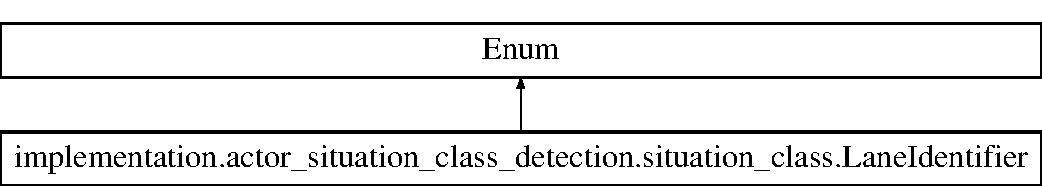
\includegraphics[height=2.000000cm]{classimplementation_1_1actor__situation__class__detection_1_1situation__class_1_1_lane_identifier}
\end{center}
\end{figure}
\subsection*{Static Public Attributes}
\begin{DoxyCompactItemize}
\item 
int \hyperlink{classimplementation_1_1actor__situation__class__detection_1_1situation__class_1_1_lane_identifier_afb2a2210286b5f946a42f3ed9432ae37}{L\+E\+F\+T\+\_\+\+L\+A\+NE} = 1
\item 
int \hyperlink{classimplementation_1_1actor__situation__class__detection_1_1situation__class_1_1_lane_identifier_a375985233368b3d3db7fe07f75e6225e}{R\+I\+G\+H\+T\+\_\+\+L\+A\+NE} = 2
\item 
int \hyperlink{classimplementation_1_1actor__situation__class__detection_1_1situation__class_1_1_lane_identifier_a5cea2450db27fc0da7a46789b5ac93a5}{N\+O\+T\+\_\+\+S\+P\+E\+C\+I\+F\+I\+ED} = 3
\end{DoxyCompactItemize}


\subsection{Member Data Documentation}
\mbox{\Hypertarget{classimplementation_1_1actor__situation__class__detection_1_1situation__class_1_1_lane_identifier_afb2a2210286b5f946a42f3ed9432ae37}\label{classimplementation_1_1actor__situation__class__detection_1_1situation__class_1_1_lane_identifier_afb2a2210286b5f946a42f3ed9432ae37}} 
\index{implementation\+::actor\+\_\+situation\+\_\+class\+\_\+detection\+::situation\+\_\+class\+::\+Lane\+Identifier@{implementation\+::actor\+\_\+situation\+\_\+class\+\_\+detection\+::situation\+\_\+class\+::\+Lane\+Identifier}!L\+E\+F\+T\+\_\+\+L\+A\+NE@{L\+E\+F\+T\+\_\+\+L\+A\+NE}}
\index{L\+E\+F\+T\+\_\+\+L\+A\+NE@{L\+E\+F\+T\+\_\+\+L\+A\+NE}!implementation\+::actor\+\_\+situation\+\_\+class\+\_\+detection\+::situation\+\_\+class\+::\+Lane\+Identifier@{implementation\+::actor\+\_\+situation\+\_\+class\+\_\+detection\+::situation\+\_\+class\+::\+Lane\+Identifier}}
\subsubsection{\texorpdfstring{L\+E\+F\+T\+\_\+\+L\+A\+NE}{LEFT\_LANE}}
{\footnotesize\ttfamily int implementation.\+actor\+\_\+situation\+\_\+class\+\_\+detection.\+situation\+\_\+class.\+Lane\+Identifier.\+L\+E\+F\+T\+\_\+\+L\+A\+NE = 1\hspace{0.3cm}{\ttfamily [static]}}

\mbox{\Hypertarget{classimplementation_1_1actor__situation__class__detection_1_1situation__class_1_1_lane_identifier_a5cea2450db27fc0da7a46789b5ac93a5}\label{classimplementation_1_1actor__situation__class__detection_1_1situation__class_1_1_lane_identifier_a5cea2450db27fc0da7a46789b5ac93a5}} 
\index{implementation\+::actor\+\_\+situation\+\_\+class\+\_\+detection\+::situation\+\_\+class\+::\+Lane\+Identifier@{implementation\+::actor\+\_\+situation\+\_\+class\+\_\+detection\+::situation\+\_\+class\+::\+Lane\+Identifier}!N\+O\+T\+\_\+\+S\+P\+E\+C\+I\+F\+I\+ED@{N\+O\+T\+\_\+\+S\+P\+E\+C\+I\+F\+I\+ED}}
\index{N\+O\+T\+\_\+\+S\+P\+E\+C\+I\+F\+I\+ED@{N\+O\+T\+\_\+\+S\+P\+E\+C\+I\+F\+I\+ED}!implementation\+::actor\+\_\+situation\+\_\+class\+\_\+detection\+::situation\+\_\+class\+::\+Lane\+Identifier@{implementation\+::actor\+\_\+situation\+\_\+class\+\_\+detection\+::situation\+\_\+class\+::\+Lane\+Identifier}}
\subsubsection{\texorpdfstring{N\+O\+T\+\_\+\+S\+P\+E\+C\+I\+F\+I\+ED}{NOT\_SPECIFIED}}
{\footnotesize\ttfamily int implementation.\+actor\+\_\+situation\+\_\+class\+\_\+detection.\+situation\+\_\+class.\+Lane\+Identifier.\+N\+O\+T\+\_\+\+S\+P\+E\+C\+I\+F\+I\+ED = 3\hspace{0.3cm}{\ttfamily [static]}}

\mbox{\Hypertarget{classimplementation_1_1actor__situation__class__detection_1_1situation__class_1_1_lane_identifier_a375985233368b3d3db7fe07f75e6225e}\label{classimplementation_1_1actor__situation__class__detection_1_1situation__class_1_1_lane_identifier_a375985233368b3d3db7fe07f75e6225e}} 
\index{implementation\+::actor\+\_\+situation\+\_\+class\+\_\+detection\+::situation\+\_\+class\+::\+Lane\+Identifier@{implementation\+::actor\+\_\+situation\+\_\+class\+\_\+detection\+::situation\+\_\+class\+::\+Lane\+Identifier}!R\+I\+G\+H\+T\+\_\+\+L\+A\+NE@{R\+I\+G\+H\+T\+\_\+\+L\+A\+NE}}
\index{R\+I\+G\+H\+T\+\_\+\+L\+A\+NE@{R\+I\+G\+H\+T\+\_\+\+L\+A\+NE}!implementation\+::actor\+\_\+situation\+\_\+class\+\_\+detection\+::situation\+\_\+class\+::\+Lane\+Identifier@{implementation\+::actor\+\_\+situation\+\_\+class\+\_\+detection\+::situation\+\_\+class\+::\+Lane\+Identifier}}
\subsubsection{\texorpdfstring{R\+I\+G\+H\+T\+\_\+\+L\+A\+NE}{RIGHT\_LANE}}
{\footnotesize\ttfamily int implementation.\+actor\+\_\+situation\+\_\+class\+\_\+detection.\+situation\+\_\+class.\+Lane\+Identifier.\+R\+I\+G\+H\+T\+\_\+\+L\+A\+NE = 2\hspace{0.3cm}{\ttfamily [static]}}



The documentation for this class was generated from the following file\+:\begin{DoxyCompactItemize}
\item 
implementation/actor\+\_\+situation\+\_\+class\+\_\+detection/\hyperlink{situation__class_8py}{situation\+\_\+class.\+py}\end{DoxyCompactItemize}

\hypertarget{classimplementation_1_1manual__control_1_1_lane_invasion_sensor}{}\doxysection{implementation.\+manual\+\_\+control.\+Lane\+Invasion\+Sensor Class Reference}
\label{classimplementation_1_1manual__control_1_1_lane_invasion_sensor}\index{implementation.manual\_control.LaneInvasionSensor@{implementation.manual\_control.LaneInvasionSensor}}
Inheritance diagram for implementation.\+manual\+\_\+control.\+Lane\+Invasion\+Sensor\+:\begin{figure}[H]
\begin{center}
\leavevmode
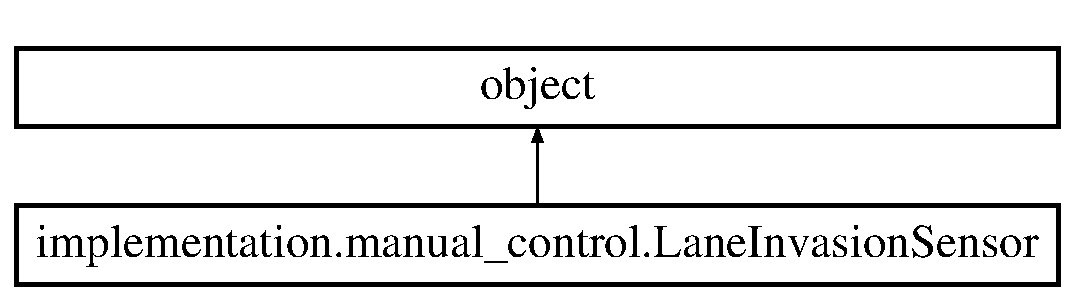
\includegraphics[height=2.000000cm]{classimplementation_1_1manual__control_1_1_lane_invasion_sensor}
\end{center}
\end{figure}
\doxysubsection*{Public Member Functions}
\begin{DoxyCompactItemize}
\item 
def \mbox{\hyperlink{classimplementation_1_1manual__control_1_1_lane_invasion_sensor_a0b38f5a85365c77a41168aa36ec27dea}{\+\_\+\+\_\+init\+\_\+\+\_\+}} (self, parent\+\_\+actor, \mbox{\hyperlink{classimplementation_1_1manual__control_1_1_lane_invasion_sensor_a87ade23d06b806a2e384b182fa682ca7}{hud}})
\end{DoxyCompactItemize}
\doxysubsection*{Public Attributes}
\begin{DoxyCompactItemize}
\item 
\mbox{\hyperlink{classimplementation_1_1manual__control_1_1_lane_invasion_sensor_a0b3804bbe4ff1fd641df8612768d2948}{sensor}}
\item 
\mbox{\hyperlink{classimplementation_1_1manual__control_1_1_lane_invasion_sensor_a87ade23d06b806a2e384b182fa682ca7}{hud}}
\end{DoxyCompactItemize}


\doxysubsection{Constructor \& Destructor Documentation}
\mbox{\Hypertarget{classimplementation_1_1manual__control_1_1_lane_invasion_sensor_a0b38f5a85365c77a41168aa36ec27dea}\label{classimplementation_1_1manual__control_1_1_lane_invasion_sensor_a0b38f5a85365c77a41168aa36ec27dea}} 
\index{implementation.manual\_control.LaneInvasionSensor@{implementation.manual\_control.LaneInvasionSensor}!\_\_init\_\_@{\_\_init\_\_}}
\index{\_\_init\_\_@{\_\_init\_\_}!implementation.manual\_control.LaneInvasionSensor@{implementation.manual\_control.LaneInvasionSensor}}
\doxysubsubsection{\texorpdfstring{\_\_init\_\_()}{\_\_init\_\_()}}
{\footnotesize\ttfamily def implementation.\+manual\+\_\+control.\+Lane\+Invasion\+Sensor.\+\_\+\+\_\+init\+\_\+\+\_\+ (\begin{DoxyParamCaption}\item[{}]{self,  }\item[{}]{parent\+\_\+actor,  }\item[{}]{hud }\end{DoxyParamCaption})}



\doxysubsection{Member Data Documentation}
\mbox{\Hypertarget{classimplementation_1_1manual__control_1_1_lane_invasion_sensor_a87ade23d06b806a2e384b182fa682ca7}\label{classimplementation_1_1manual__control_1_1_lane_invasion_sensor_a87ade23d06b806a2e384b182fa682ca7}} 
\index{implementation.manual\_control.LaneInvasionSensor@{implementation.manual\_control.LaneInvasionSensor}!hud@{hud}}
\index{hud@{hud}!implementation.manual\_control.LaneInvasionSensor@{implementation.manual\_control.LaneInvasionSensor}}
\doxysubsubsection{\texorpdfstring{hud}{hud}}
{\footnotesize\ttfamily implementation.\+manual\+\_\+control.\+Lane\+Invasion\+Sensor.\+hud}

\mbox{\Hypertarget{classimplementation_1_1manual__control_1_1_lane_invasion_sensor_a0b3804bbe4ff1fd641df8612768d2948}\label{classimplementation_1_1manual__control_1_1_lane_invasion_sensor_a0b3804bbe4ff1fd641df8612768d2948}} 
\index{implementation.manual\_control.LaneInvasionSensor@{implementation.manual\_control.LaneInvasionSensor}!sensor@{sensor}}
\index{sensor@{sensor}!implementation.manual\_control.LaneInvasionSensor@{implementation.manual\_control.LaneInvasionSensor}}
\doxysubsubsection{\texorpdfstring{sensor}{sensor}}
{\footnotesize\ttfamily implementation.\+manual\+\_\+control.\+Lane\+Invasion\+Sensor.\+sensor}



The documentation for this class was generated from the following file\+:\begin{DoxyCompactItemize}
\item 
implementation/\mbox{\hyperlink{manual__control_8py}{manual\+\_\+control.\+py}}\end{DoxyCompactItemize}

\hypertarget{classimplementation_1_1data__model_1_1positions_1_1_lane_position}{}\section{implementation.\+data\+\_\+model.\+positions.\+Lane\+Position Class Reference}
\label{classimplementation_1_1data__model_1_1positions_1_1_lane_position}\index{implementation.\+data\+\_\+model.\+positions.\+Lane\+Position@{implementation.\+data\+\_\+model.\+positions.\+Lane\+Position}}
\subsection*{Static Public Attributes}
\begin{DoxyCompactItemize}
\item 
\hyperlink{classimplementation_1_1data__model_1_1positions_1_1_lane_position_ac9c876221453d49a2c5414cd415749f2}{str}
\item 
\hyperlink{classimplementation_1_1data__model_1_1positions_1_1_lane_position_a09c02454c62ee6bb98ceeac42db071fc}{float}
\item 
\hyperlink{classimplementation_1_1data__model_1_1positions_1_1_lane_position_a93831a9eeb1d5a073bbd0e30c8aec569}{Orientation}
\end{DoxyCompactItemize}


\subsection{Detailed Description}
\begin{DoxyVerb}Position of an entity along a Lane
Attributes
----------
laneId : str
    unique identifier of the lane
offset : float
    lateral offset to the centerline of the current lane in [m]
orientation : Orientation

roadId : str
    unique identifier of the road the lane belongs to
s : float
    current position along the lanes centerline in [m]
\end{DoxyVerb}
 

\subsection{Member Data Documentation}
\mbox{\Hypertarget{classimplementation_1_1data__model_1_1positions_1_1_lane_position_a09c02454c62ee6bb98ceeac42db071fc}\label{classimplementation_1_1data__model_1_1positions_1_1_lane_position_a09c02454c62ee6bb98ceeac42db071fc}} 
\index{implementation\+::data\+\_\+model\+::positions\+::\+Lane\+Position@{implementation\+::data\+\_\+model\+::positions\+::\+Lane\+Position}!float@{float}}
\index{float@{float}!implementation\+::data\+\_\+model\+::positions\+::\+Lane\+Position@{implementation\+::data\+\_\+model\+::positions\+::\+Lane\+Position}}
\subsubsection{\texorpdfstring{float}{float}}
{\footnotesize\ttfamily implementation.\+data\+\_\+model.\+positions.\+Lane\+Position.\+float\hspace{0.3cm}{\ttfamily [static]}}

\mbox{\Hypertarget{classimplementation_1_1data__model_1_1positions_1_1_lane_position_a93831a9eeb1d5a073bbd0e30c8aec569}\label{classimplementation_1_1data__model_1_1positions_1_1_lane_position_a93831a9eeb1d5a073bbd0e30c8aec569}} 
\index{implementation\+::data\+\_\+model\+::positions\+::\+Lane\+Position@{implementation\+::data\+\_\+model\+::positions\+::\+Lane\+Position}!Orientation@{Orientation}}
\index{Orientation@{Orientation}!implementation\+::data\+\_\+model\+::positions\+::\+Lane\+Position@{implementation\+::data\+\_\+model\+::positions\+::\+Lane\+Position}}
\subsubsection{\texorpdfstring{Orientation}{Orientation}}
{\footnotesize\ttfamily implementation.\+data\+\_\+model.\+positions.\+Lane\+Position.\+Orientation\hspace{0.3cm}{\ttfamily [static]}}

\mbox{\Hypertarget{classimplementation_1_1data__model_1_1positions_1_1_lane_position_ac9c876221453d49a2c5414cd415749f2}\label{classimplementation_1_1data__model_1_1positions_1_1_lane_position_ac9c876221453d49a2c5414cd415749f2}} 
\index{implementation\+::data\+\_\+model\+::positions\+::\+Lane\+Position@{implementation\+::data\+\_\+model\+::positions\+::\+Lane\+Position}!str@{str}}
\index{str@{str}!implementation\+::data\+\_\+model\+::positions\+::\+Lane\+Position@{implementation\+::data\+\_\+model\+::positions\+::\+Lane\+Position}}
\subsubsection{\texorpdfstring{str}{str}}
{\footnotesize\ttfamily implementation.\+data\+\_\+model.\+positions.\+Lane\+Position.\+str\hspace{0.3cm}{\ttfamily [static]}}



The documentation for this class was generated from the following file\+:\begin{DoxyCompactItemize}
\item 
implementation/data\+\_\+model/\hyperlink{positions_8py}{positions.\+py}\end{DoxyCompactItemize}

\hypertarget{classimplementation_1_1data__model_1_1positions_1_1_location}{}\section{implementation.\+data\+\_\+model.\+positions.\+Location Class Reference}
\label{classimplementation_1_1data__model_1_1positions_1_1_location}\index{implementation.\+data\+\_\+model.\+positions.\+Location@{implementation.\+data\+\_\+model.\+positions.\+Location}}
Inheritance diagram for implementation.\+data\+\_\+model.\+positions.\+Location\+:\begin{figure}[H]
\begin{center}
\leavevmode
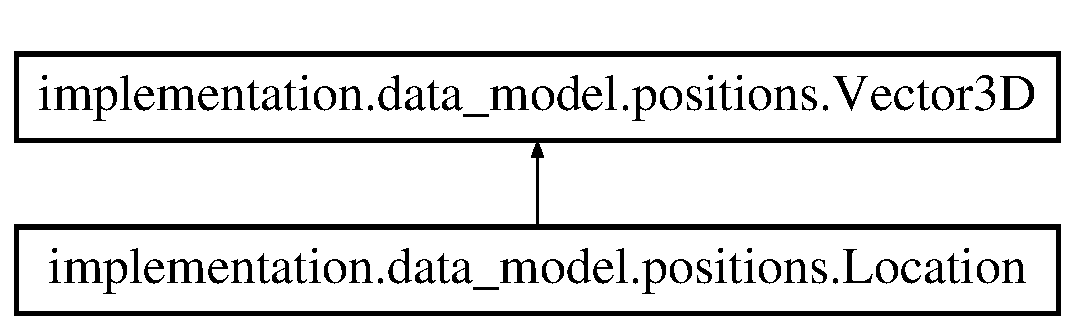
\includegraphics[height=2.000000cm]{classimplementation_1_1data__model_1_1positions_1_1_location}
\end{center}
\end{figure}
\subsection*{Public Member Functions}
\begin{DoxyCompactItemize}
\item 
def \hyperlink{classimplementation_1_1data__model_1_1positions_1_1_location_aadfa22fb1aece1c971622d353ead8f52}{to\+\_\+\+E\+NU} (self)
\item 
def \hyperlink{classimplementation_1_1data__model_1_1positions_1_1_location_a527219476defb5b0d133753d6dd9e38b}{E\+N\+U\+\_\+to\+\_\+location}
\item 
def \hyperlink{classimplementation_1_1data__model_1_1positions_1_1_location_ae478f2b341a8cdd685749d8361b12223}{get\+\_\+2d\+\_\+distance}
\item 
def \hyperlink{classimplementation_1_1data__model_1_1positions_1_1_location_a3be0c075e6034c53b3319441efd28531}{distance}
\item 
def \hyperlink{classimplementation_1_1data__model_1_1positions_1_1_location_a5fc17326206c227594522dcaefed081c}{invert} (self)
\end{DoxyCompactItemize}
\subsection*{Additional Inherited Members}


\subsection{Member Function Documentation}
\mbox{\Hypertarget{classimplementation_1_1data__model_1_1positions_1_1_location_a3be0c075e6034c53b3319441efd28531}\label{classimplementation_1_1data__model_1_1positions_1_1_location_a3be0c075e6034c53b3319441efd28531}} 
\index{implementation\+::data\+\_\+model\+::positions\+::\+Location@{implementation\+::data\+\_\+model\+::positions\+::\+Location}!distance@{distance}}
\index{distance@{distance}!implementation\+::data\+\_\+model\+::positions\+::\+Location@{implementation\+::data\+\_\+model\+::positions\+::\+Location}}
\subsubsection{\texorpdfstring{distance()}{distance()}}
{\footnotesize\ttfamily def implementation.\+data\+\_\+model.\+positions.\+Location.\+distance (\begin{DoxyParamCaption}\item[{}]{self,  }\item[{}]{other\+\_\+location }\end{DoxyParamCaption})}

\mbox{\Hypertarget{classimplementation_1_1data__model_1_1positions_1_1_location_a527219476defb5b0d133753d6dd9e38b}\label{classimplementation_1_1data__model_1_1positions_1_1_location_a527219476defb5b0d133753d6dd9e38b}} 
\index{implementation\+::data\+\_\+model\+::positions\+::\+Location@{implementation\+::data\+\_\+model\+::positions\+::\+Location}!E\+N\+U\+\_\+to\+\_\+location@{E\+N\+U\+\_\+to\+\_\+location}}
\index{E\+N\+U\+\_\+to\+\_\+location@{E\+N\+U\+\_\+to\+\_\+location}!implementation\+::data\+\_\+model\+::positions\+::\+Location@{implementation\+::data\+\_\+model\+::positions\+::\+Location}}
\subsubsection{\texorpdfstring{E\+N\+U\+\_\+to\+\_\+location()}{ENU\_to\_location()}}
{\footnotesize\ttfamily def implementation.\+data\+\_\+model.\+positions.\+Location.\+E\+N\+U\+\_\+to\+\_\+location (\begin{DoxyParamCaption}\item[{}]{self,  }\item[{}]{enu\+\_\+point }\end{DoxyParamCaption})}

\mbox{\Hypertarget{classimplementation_1_1data__model_1_1positions_1_1_location_ae478f2b341a8cdd685749d8361b12223}\label{classimplementation_1_1data__model_1_1positions_1_1_location_ae478f2b341a8cdd685749d8361b12223}} 
\index{implementation\+::data\+\_\+model\+::positions\+::\+Location@{implementation\+::data\+\_\+model\+::positions\+::\+Location}!get\+\_\+2d\+\_\+distance@{get\+\_\+2d\+\_\+distance}}
\index{get\+\_\+2d\+\_\+distance@{get\+\_\+2d\+\_\+distance}!implementation\+::data\+\_\+model\+::positions\+::\+Location@{implementation\+::data\+\_\+model\+::positions\+::\+Location}}
\subsubsection{\texorpdfstring{get\+\_\+2d\+\_\+distance()}{get\_2d\_distance()}}
{\footnotesize\ttfamily def implementation.\+data\+\_\+model.\+positions.\+Location.\+get\+\_\+2d\+\_\+distance (\begin{DoxyParamCaption}\item[{}]{self,  }\item[{}]{other\+\_\+location }\end{DoxyParamCaption})}

\mbox{\Hypertarget{classimplementation_1_1data__model_1_1positions_1_1_location_a5fc17326206c227594522dcaefed081c}\label{classimplementation_1_1data__model_1_1positions_1_1_location_a5fc17326206c227594522dcaefed081c}} 
\index{implementation\+::data\+\_\+model\+::positions\+::\+Location@{implementation\+::data\+\_\+model\+::positions\+::\+Location}!invert@{invert}}
\index{invert@{invert}!implementation\+::data\+\_\+model\+::positions\+::\+Location@{implementation\+::data\+\_\+model\+::positions\+::\+Location}}
\subsubsection{\texorpdfstring{invert()}{invert()}}
{\footnotesize\ttfamily def implementation.\+data\+\_\+model.\+positions.\+Location.\+invert (\begin{DoxyParamCaption}\item[{}]{self,  }\item[{}]{Location }\end{DoxyParamCaption})}

\begin{DoxyVerb}Returns the inverted Location

Returns
-------
Location
    Inverted Location\end{DoxyVerb}
 \mbox{\Hypertarget{classimplementation_1_1data__model_1_1positions_1_1_location_aadfa22fb1aece1c971622d353ead8f52}\label{classimplementation_1_1data__model_1_1positions_1_1_location_aadfa22fb1aece1c971622d353ead8f52}} 
\index{implementation\+::data\+\_\+model\+::positions\+::\+Location@{implementation\+::data\+\_\+model\+::positions\+::\+Location}!to\+\_\+\+E\+NU@{to\+\_\+\+E\+NU}}
\index{to\+\_\+\+E\+NU@{to\+\_\+\+E\+NU}!implementation\+::data\+\_\+model\+::positions\+::\+Location@{implementation\+::data\+\_\+model\+::positions\+::\+Location}}
\subsubsection{\texorpdfstring{to\+\_\+\+E\+N\+U()}{to\_ENU()}}
{\footnotesize\ttfamily def implementation.\+data\+\_\+model.\+positions.\+Location.\+to\+\_\+\+E\+NU (\begin{DoxyParamCaption}\item[{}]{self,  }\item[{}]{ad,  }\item[{}]{map,  }\item[{}]{point,  }\item[{}]{E\+N\+U\+Point }\end{DoxyParamCaption})}

\begin{DoxyVerb}Returns an ENU Point of the Location

Returns
-------
ad.map.point.ENUPoint
    ENU Point of the Location\end{DoxyVerb}
 

The documentation for this class was generated from the following file\+:\begin{DoxyCompactItemize}
\item 
implementation/data\+\_\+model/\hyperlink{positions_8py}{positions.\+py}\end{DoxyCompactItemize}

\hypertarget{classimplementation_1_1data__model_1_1map_1_1_map}{}\section{implementation.\+data\+\_\+model.\+map.\+Map Class Reference}
\label{classimplementation_1_1data__model_1_1map_1_1_map}\index{implementation.\+data\+\_\+model.\+map.\+Map@{implementation.\+data\+\_\+model.\+map.\+Map}}
Inheritance diagram for implementation.\+data\+\_\+model.\+map.\+Map\+:\begin{figure}[H]
\begin{center}
\leavevmode
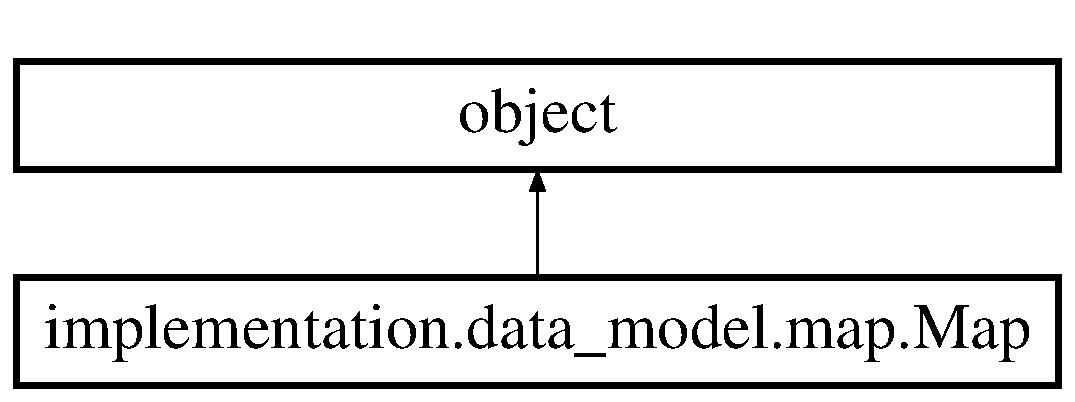
\includegraphics[height=2.000000cm]{classimplementation_1_1data__model_1_1map_1_1_map}
\end{center}
\end{figure}
\subsection*{Public Member Functions}
\begin{DoxyCompactItemize}
\item 
def \hyperlink{classimplementation_1_1data__model_1_1map_1_1_map_a4fc6942eed69c519ac3b34ff2ff0a92d}{\+\_\+\+\_\+init\+\_\+\+\_\+} (self, map\+\_\+name)
\item 
def \hyperlink{classimplementation_1_1data__model_1_1map_1_1_map_aa594532ade53c7e6ec730e657e383271}{get\+\_\+distance\+\_\+to\+\_\+lane\+\_\+end}
\item 
def \hyperlink{classimplementation_1_1data__model_1_1map_1_1_map_a03736a8ebf18a875f53992b977736108}{get\+\_\+waypoint}
\item 
def \hyperlink{classimplementation_1_1data__model_1_1map_1_1_map_a815310646f53527f0be529d336b0317c}{get\+\_\+point\+\_\+on\+\_\+lane\+\_\+right}
\item 
def \hyperlink{classimplementation_1_1data__model_1_1map_1_1_map_a799206c287976e7291ffbe509c3754ce}{get\+\_\+point\+\_\+on\+\_\+lane\+\_\+left}
\item 
def \hyperlink{classimplementation_1_1data__model_1_1map_1_1_map_afc749937439c4c831c1061928563030a}{get\+\_\+next\+\_\+point\+\_\+on\+\_\+lane}
\end{DoxyCompactItemize}
\subsection*{Public Attributes}
\begin{DoxyCompactItemize}
\item 
\hyperlink{classimplementation_1_1data__model_1_1map_1_1_map_a9c9d66086867f8a00ed50f814a4323b1}{map}
\item 
\hyperlink{classimplementation_1_1data__model_1_1map_1_1_map_a0a36c23f92da7063d8377fc83c373128}{map\+\_\+matching}
\end{DoxyCompactItemize}


\subsection{Detailed Description}
\begin{DoxyVerb}Map class that holds a representation of the ad map and provides severel functions to work with the map.
Takes the map name of the current town to create an ad representation.

Attributes;
map : ad.map
    ad map object of the current map
map_matching : ad.map.match.AdMapMatching
    Object that handles all map matching actions
\end{DoxyVerb}
 

\subsection{Constructor \& Destructor Documentation}
\mbox{\Hypertarget{classimplementation_1_1data__model_1_1map_1_1_map_a4fc6942eed69c519ac3b34ff2ff0a92d}\label{classimplementation_1_1data__model_1_1map_1_1_map_a4fc6942eed69c519ac3b34ff2ff0a92d}} 
\index{implementation\+::data\+\_\+model\+::map\+::\+Map@{implementation\+::data\+\_\+model\+::map\+::\+Map}!\+\_\+\+\_\+init\+\_\+\+\_\+@{\+\_\+\+\_\+init\+\_\+\+\_\+}}
\index{\+\_\+\+\_\+init\+\_\+\+\_\+@{\+\_\+\+\_\+init\+\_\+\+\_\+}!implementation\+::data\+\_\+model\+::map\+::\+Map@{implementation\+::data\+\_\+model\+::map\+::\+Map}}
\subsubsection{\texorpdfstring{\+\_\+\+\_\+init\+\_\+\+\_\+()}{\_\_init\_\_()}}
{\footnotesize\ttfamily def implementation.\+data\+\_\+model.\+map.\+Map.\+\_\+\+\_\+init\+\_\+\+\_\+ (\begin{DoxyParamCaption}\item[{}]{self,  }\item[{}]{map\+\_\+name }\end{DoxyParamCaption})}

\begin{DoxyVerb}Constructor for the Map class. Loads the ad map from an OpenDrive File

Parameters
----------
map_name : str
    Name of the map (i.e. Town03) without .xodr
\end{DoxyVerb}
 

\subsection{Member Function Documentation}
\mbox{\Hypertarget{classimplementation_1_1data__model_1_1map_1_1_map_aa594532ade53c7e6ec730e657e383271}\label{classimplementation_1_1data__model_1_1map_1_1_map_aa594532ade53c7e6ec730e657e383271}} 
\index{implementation\+::data\+\_\+model\+::map\+::\+Map@{implementation\+::data\+\_\+model\+::map\+::\+Map}!get\+\_\+distance\+\_\+to\+\_\+lane\+\_\+end@{get\+\_\+distance\+\_\+to\+\_\+lane\+\_\+end}}
\index{get\+\_\+distance\+\_\+to\+\_\+lane\+\_\+end@{get\+\_\+distance\+\_\+to\+\_\+lane\+\_\+end}!implementation\+::data\+\_\+model\+::map\+::\+Map@{implementation\+::data\+\_\+model\+::map\+::\+Map}}
\subsubsection{\texorpdfstring{get\+\_\+distance\+\_\+to\+\_\+lane\+\_\+end()}{get\_distance\_to\_lane\_end()}}
{\footnotesize\ttfamily def implementation.\+data\+\_\+model.\+map.\+Map.\+get\+\_\+distance\+\_\+to\+\_\+lane\+\_\+end (\begin{DoxyParamCaption}\item[{}]{self,  }\item[{}]{location }\end{DoxyParamCaption})}

\mbox{\Hypertarget{classimplementation_1_1data__model_1_1map_1_1_map_afc749937439c4c831c1061928563030a}\label{classimplementation_1_1data__model_1_1map_1_1_map_afc749937439c4c831c1061928563030a}} 
\index{implementation\+::data\+\_\+model\+::map\+::\+Map@{implementation\+::data\+\_\+model\+::map\+::\+Map}!get\+\_\+next\+\_\+point\+\_\+on\+\_\+lane@{get\+\_\+next\+\_\+point\+\_\+on\+\_\+lane}}
\index{get\+\_\+next\+\_\+point\+\_\+on\+\_\+lane@{get\+\_\+next\+\_\+point\+\_\+on\+\_\+lane}!implementation\+::data\+\_\+model\+::map\+::\+Map@{implementation\+::data\+\_\+model\+::map\+::\+Map}}
\subsubsection{\texorpdfstring{get\+\_\+next\+\_\+point\+\_\+on\+\_\+lane()}{get\_next\_point\_on\_lane()}}
{\footnotesize\ttfamily def implementation.\+data\+\_\+model.\+map.\+Map.\+get\+\_\+next\+\_\+point\+\_\+on\+\_\+lane (\begin{DoxyParamCaption}\item[{}]{self,  }\item[{}]{start\+\_\+point }\end{DoxyParamCaption})}

\mbox{\Hypertarget{classimplementation_1_1data__model_1_1map_1_1_map_a799206c287976e7291ffbe509c3754ce}\label{classimplementation_1_1data__model_1_1map_1_1_map_a799206c287976e7291ffbe509c3754ce}} 
\index{implementation\+::data\+\_\+model\+::map\+::\+Map@{implementation\+::data\+\_\+model\+::map\+::\+Map}!get\+\_\+point\+\_\+on\+\_\+lane\+\_\+left@{get\+\_\+point\+\_\+on\+\_\+lane\+\_\+left}}
\index{get\+\_\+point\+\_\+on\+\_\+lane\+\_\+left@{get\+\_\+point\+\_\+on\+\_\+lane\+\_\+left}!implementation\+::data\+\_\+model\+::map\+::\+Map@{implementation\+::data\+\_\+model\+::map\+::\+Map}}
\subsubsection{\texorpdfstring{get\+\_\+point\+\_\+on\+\_\+lane\+\_\+left()}{get\_point\_on\_lane\_left()}}
{\footnotesize\ttfamily def implementation.\+data\+\_\+model.\+map.\+Map.\+get\+\_\+point\+\_\+on\+\_\+lane\+\_\+left (\begin{DoxyParamCaption}\item[{}]{self,  }\item[{}]{location }\end{DoxyParamCaption})}

\mbox{\Hypertarget{classimplementation_1_1data__model_1_1map_1_1_map_a815310646f53527f0be529d336b0317c}\label{classimplementation_1_1data__model_1_1map_1_1_map_a815310646f53527f0be529d336b0317c}} 
\index{implementation\+::data\+\_\+model\+::map\+::\+Map@{implementation\+::data\+\_\+model\+::map\+::\+Map}!get\+\_\+point\+\_\+on\+\_\+lane\+\_\+right@{get\+\_\+point\+\_\+on\+\_\+lane\+\_\+right}}
\index{get\+\_\+point\+\_\+on\+\_\+lane\+\_\+right@{get\+\_\+point\+\_\+on\+\_\+lane\+\_\+right}!implementation\+::data\+\_\+model\+::map\+::\+Map@{implementation\+::data\+\_\+model\+::map\+::\+Map}}
\subsubsection{\texorpdfstring{get\+\_\+point\+\_\+on\+\_\+lane\+\_\+right()}{get\_point\_on\_lane\_right()}}
{\footnotesize\ttfamily def implementation.\+data\+\_\+model.\+map.\+Map.\+get\+\_\+point\+\_\+on\+\_\+lane\+\_\+right (\begin{DoxyParamCaption}\item[{}]{self,  }\item[{}]{location }\end{DoxyParamCaption})}

\mbox{\Hypertarget{classimplementation_1_1data__model_1_1map_1_1_map_a03736a8ebf18a875f53992b977736108}\label{classimplementation_1_1data__model_1_1map_1_1_map_a03736a8ebf18a875f53992b977736108}} 
\index{implementation\+::data\+\_\+model\+::map\+::\+Map@{implementation\+::data\+\_\+model\+::map\+::\+Map}!get\+\_\+waypoint@{get\+\_\+waypoint}}
\index{get\+\_\+waypoint@{get\+\_\+waypoint}!implementation\+::data\+\_\+model\+::map\+::\+Map@{implementation\+::data\+\_\+model\+::map\+::\+Map}}
\subsubsection{\texorpdfstring{get\+\_\+waypoint()}{get\_waypoint()}}
{\footnotesize\ttfamily def implementation.\+data\+\_\+model.\+map.\+Map.\+get\+\_\+waypoint (\begin{DoxyParamCaption}\item[{}]{self,  }\item[{}]{location }\end{DoxyParamCaption})}



\subsection{Member Data Documentation}
\mbox{\Hypertarget{classimplementation_1_1data__model_1_1map_1_1_map_a9c9d66086867f8a00ed50f814a4323b1}\label{classimplementation_1_1data__model_1_1map_1_1_map_a9c9d66086867f8a00ed50f814a4323b1}} 
\index{implementation\+::data\+\_\+model\+::map\+::\+Map@{implementation\+::data\+\_\+model\+::map\+::\+Map}!map@{map}}
\index{map@{map}!implementation\+::data\+\_\+model\+::map\+::\+Map@{implementation\+::data\+\_\+model\+::map\+::\+Map}}
\subsubsection{\texorpdfstring{map}{map}}
{\footnotesize\ttfamily implementation.\+data\+\_\+model.\+map.\+Map.\+map}

\mbox{\Hypertarget{classimplementation_1_1data__model_1_1map_1_1_map_a0a36c23f92da7063d8377fc83c373128}\label{classimplementation_1_1data__model_1_1map_1_1_map_a0a36c23f92da7063d8377fc83c373128}} 
\index{implementation\+::data\+\_\+model\+::map\+::\+Map@{implementation\+::data\+\_\+model\+::map\+::\+Map}!map\+\_\+matching@{map\+\_\+matching}}
\index{map\+\_\+matching@{map\+\_\+matching}!implementation\+::data\+\_\+model\+::map\+::\+Map@{implementation\+::data\+\_\+model\+::map\+::\+Map}}
\subsubsection{\texorpdfstring{map\+\_\+matching}{map\_matching}}
{\footnotesize\ttfamily implementation.\+data\+\_\+model.\+map.\+Map.\+map\+\_\+matching}



The documentation for this class was generated from the following file\+:\begin{DoxyCompactItemize}
\item 
implementation/data\+\_\+model/\hyperlink{map_8py}{map.\+py}\end{DoxyCompactItemize}

\hypertarget{classimplementation_1_1data__model_1_1entity_1_1_misc_object}{}\section{implementation.\+data\+\_\+model.\+entity.\+Misc\+Object Class Reference}
\label{classimplementation_1_1data__model_1_1entity_1_1_misc_object}\index{implementation.\+data\+\_\+model.\+entity.\+Misc\+Object@{implementation.\+data\+\_\+model.\+entity.\+Misc\+Object}}
Inheritance diagram for implementation.\+data\+\_\+model.\+entity.\+Misc\+Object\+:\begin{figure}[H]
\begin{center}
\leavevmode
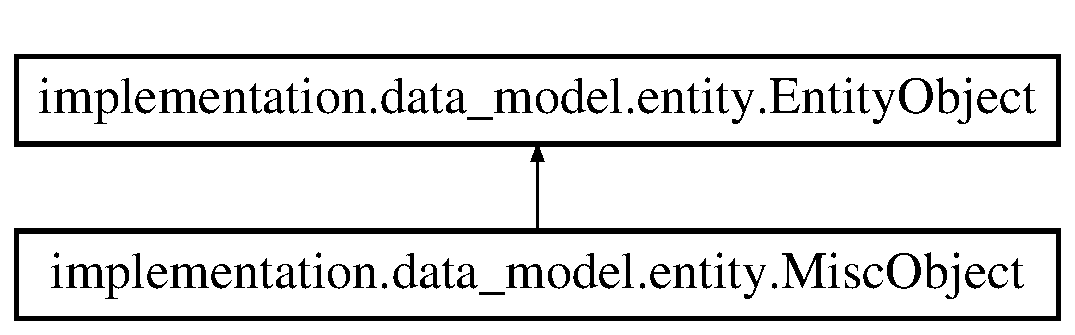
\includegraphics[height=2.000000cm]{classimplementation_1_1data__model_1_1entity_1_1_misc_object}
\end{center}
\end{figure}
\subsection*{Static Public Attributes}
\begin{DoxyCompactItemize}
\item 
\hyperlink{classimplementation_1_1data__model_1_1entity_1_1_misc_object_a4bc5378ce8b7877de2ffadbe3c889bcf}{Misc\+Object\+Category}
\end{DoxyCompactItemize}
\subsection*{Additional Inherited Members}


\subsection{Member Data Documentation}
\mbox{\Hypertarget{classimplementation_1_1data__model_1_1entity_1_1_misc_object_a4bc5378ce8b7877de2ffadbe3c889bcf}\label{classimplementation_1_1data__model_1_1entity_1_1_misc_object_a4bc5378ce8b7877de2ffadbe3c889bcf}} 
\index{implementation\+::data\+\_\+model\+::entity\+::\+Misc\+Object@{implementation\+::data\+\_\+model\+::entity\+::\+Misc\+Object}!Misc\+Object\+Category@{Misc\+Object\+Category}}
\index{Misc\+Object\+Category@{Misc\+Object\+Category}!implementation\+::data\+\_\+model\+::entity\+::\+Misc\+Object@{implementation\+::data\+\_\+model\+::entity\+::\+Misc\+Object}}
\subsubsection{\texorpdfstring{Misc\+Object\+Category}{MiscObjectCategory}}
{\footnotesize\ttfamily implementation.\+data\+\_\+model.\+entity.\+Misc\+Object.\+Misc\+Object\+Category\hspace{0.3cm}{\ttfamily [static]}}



The documentation for this class was generated from the following file\+:\begin{DoxyCompactItemize}
\item 
implementation/data\+\_\+model/\hyperlink{entity_8py}{entity.\+py}\end{DoxyCompactItemize}

\hypertarget{classimplementation_1_1data__model_1_1entity_1_1_misc_object_category}{}\section{implementation.\+data\+\_\+model.\+entity.\+Misc\+Object\+Category Class Reference}
\label{classimplementation_1_1data__model_1_1entity_1_1_misc_object_category}\index{implementation.\+data\+\_\+model.\+entity.\+Misc\+Object\+Category@{implementation.\+data\+\_\+model.\+entity.\+Misc\+Object\+Category}}
Inheritance diagram for implementation.\+data\+\_\+model.\+entity.\+Misc\+Object\+Category\+:\begin{figure}[H]
\begin{center}
\leavevmode
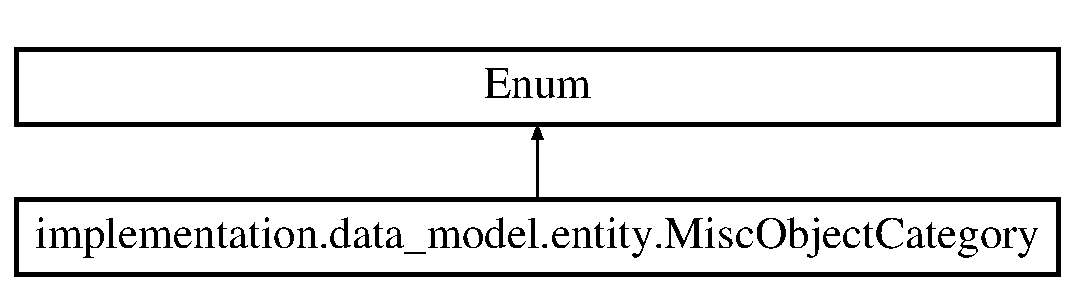
\includegraphics[height=2.000000cm]{classimplementation_1_1data__model_1_1entity_1_1_misc_object_category}
\end{center}
\end{figure}
\subsection*{Static Public Attributes}
\begin{DoxyCompactItemize}
\item 
int \hyperlink{classimplementation_1_1data__model_1_1entity_1_1_misc_object_category_afab099a879b6af98ebbafaf48f889ae3}{B\+A\+R\+R\+I\+ER} = 1
\item 
int \hyperlink{classimplementation_1_1data__model_1_1entity_1_1_misc_object_category_a861ae00367cb5000e6fc17414036c54f}{B\+U\+I\+L\+D\+I\+NG} = 2
\item 
int \hyperlink{classimplementation_1_1data__model_1_1entity_1_1_misc_object_category_a6a4397ef20c35d4a8b8cedd09d5775d4}{C\+R\+O\+S\+S\+W\+A\+LK} = 3
\item 
int \hyperlink{classimplementation_1_1data__model_1_1entity_1_1_misc_object_category_ad54abbc963f623903799a70650725085}{G\+A\+N\+T\+RY} = 4
\item 
int \hyperlink{classimplementation_1_1data__model_1_1entity_1_1_misc_object_category_a8efaa312a1a5904be8d4ea5b2e250ece}{O\+B\+S\+T\+A\+C\+LE} = 5
\item 
int \hyperlink{classimplementation_1_1data__model_1_1entity_1_1_misc_object_category_a4a1cec9a93440279a022c686fbea42a1}{P\+A\+R\+K\+I\+N\+G\+\_\+\+S\+P\+A\+CE} = 6
\item 
int \hyperlink{classimplementation_1_1data__model_1_1entity_1_1_misc_object_category_a4b4112a35bd838b10ef7f1a6d718b9e2}{P\+A\+T\+CH} = 7
\item 
int \hyperlink{classimplementation_1_1data__model_1_1entity_1_1_misc_object_category_a1ee9f34bf6efd00f6b208d1bc2a21080}{P\+O\+LE} = 8
\item 
int \hyperlink{classimplementation_1_1data__model_1_1entity_1_1_misc_object_category_adef155c599c983ba57269bdef5524731}{R\+A\+I\+L\+I\+NG} = 9
\item 
int \hyperlink{classimplementation_1_1data__model_1_1entity_1_1_misc_object_category_a368ead63b1536bc115fe49c35c2c5fb4}{R\+O\+A\+D\+\_\+\+M\+A\+RK} = 10
\item 
int \hyperlink{classimplementation_1_1data__model_1_1entity_1_1_misc_object_category_a59ed45890d63616b9c6c9588c26ee73c}{S\+O\+U\+N\+D\+\_\+\+B\+A\+R\+R\+I\+ER} = 11
\item 
int \hyperlink{classimplementation_1_1data__model_1_1entity_1_1_misc_object_category_a7f023fbe03ec4d9d9d78682d5b45e066}{S\+T\+R\+E\+E\+T\+\_\+\+L\+A\+MP} = 12
\item 
int \hyperlink{classimplementation_1_1data__model_1_1entity_1_1_misc_object_category_a5fa69706367d18a8c515ddf57f6d0f74}{T\+R\+A\+F\+F\+I\+C\+\_\+\+I\+S\+L\+A\+ND} = 13
\item 
int \hyperlink{classimplementation_1_1data__model_1_1entity_1_1_misc_object_category_a39f8825a3947c2c0f1d98aa7e67f8349}{T\+R\+EE} = 14
\item 
int \hyperlink{classimplementation_1_1data__model_1_1entity_1_1_misc_object_category_a9a279cda5b50fb0e684ac88fcaeb4b4c}{V\+E\+G\+E\+T\+A\+T\+I\+ON} = 15
\item 
int \hyperlink{classimplementation_1_1data__model_1_1entity_1_1_misc_object_category_afa34e91350db6c493e4c225b8c14404b}{N\+O\+NE} = 16
\end{DoxyCompactItemize}


\subsection{Member Data Documentation}
\mbox{\Hypertarget{classimplementation_1_1data__model_1_1entity_1_1_misc_object_category_afab099a879b6af98ebbafaf48f889ae3}\label{classimplementation_1_1data__model_1_1entity_1_1_misc_object_category_afab099a879b6af98ebbafaf48f889ae3}} 
\index{implementation\+::data\+\_\+model\+::entity\+::\+Misc\+Object\+Category@{implementation\+::data\+\_\+model\+::entity\+::\+Misc\+Object\+Category}!B\+A\+R\+R\+I\+ER@{B\+A\+R\+R\+I\+ER}}
\index{B\+A\+R\+R\+I\+ER@{B\+A\+R\+R\+I\+ER}!implementation\+::data\+\_\+model\+::entity\+::\+Misc\+Object\+Category@{implementation\+::data\+\_\+model\+::entity\+::\+Misc\+Object\+Category}}
\subsubsection{\texorpdfstring{B\+A\+R\+R\+I\+ER}{BARRIER}}
{\footnotesize\ttfamily int implementation.\+data\+\_\+model.\+entity.\+Misc\+Object\+Category.\+B\+A\+R\+R\+I\+ER = 1\hspace{0.3cm}{\ttfamily [static]}}

\mbox{\Hypertarget{classimplementation_1_1data__model_1_1entity_1_1_misc_object_category_a861ae00367cb5000e6fc17414036c54f}\label{classimplementation_1_1data__model_1_1entity_1_1_misc_object_category_a861ae00367cb5000e6fc17414036c54f}} 
\index{implementation\+::data\+\_\+model\+::entity\+::\+Misc\+Object\+Category@{implementation\+::data\+\_\+model\+::entity\+::\+Misc\+Object\+Category}!B\+U\+I\+L\+D\+I\+NG@{B\+U\+I\+L\+D\+I\+NG}}
\index{B\+U\+I\+L\+D\+I\+NG@{B\+U\+I\+L\+D\+I\+NG}!implementation\+::data\+\_\+model\+::entity\+::\+Misc\+Object\+Category@{implementation\+::data\+\_\+model\+::entity\+::\+Misc\+Object\+Category}}
\subsubsection{\texorpdfstring{B\+U\+I\+L\+D\+I\+NG}{BUILDING}}
{\footnotesize\ttfamily int implementation.\+data\+\_\+model.\+entity.\+Misc\+Object\+Category.\+B\+U\+I\+L\+D\+I\+NG = 2\hspace{0.3cm}{\ttfamily [static]}}

\mbox{\Hypertarget{classimplementation_1_1data__model_1_1entity_1_1_misc_object_category_a6a4397ef20c35d4a8b8cedd09d5775d4}\label{classimplementation_1_1data__model_1_1entity_1_1_misc_object_category_a6a4397ef20c35d4a8b8cedd09d5775d4}} 
\index{implementation\+::data\+\_\+model\+::entity\+::\+Misc\+Object\+Category@{implementation\+::data\+\_\+model\+::entity\+::\+Misc\+Object\+Category}!C\+R\+O\+S\+S\+W\+A\+LK@{C\+R\+O\+S\+S\+W\+A\+LK}}
\index{C\+R\+O\+S\+S\+W\+A\+LK@{C\+R\+O\+S\+S\+W\+A\+LK}!implementation\+::data\+\_\+model\+::entity\+::\+Misc\+Object\+Category@{implementation\+::data\+\_\+model\+::entity\+::\+Misc\+Object\+Category}}
\subsubsection{\texorpdfstring{C\+R\+O\+S\+S\+W\+A\+LK}{CROSSWALK}}
{\footnotesize\ttfamily int implementation.\+data\+\_\+model.\+entity.\+Misc\+Object\+Category.\+C\+R\+O\+S\+S\+W\+A\+LK = 3\hspace{0.3cm}{\ttfamily [static]}}

\mbox{\Hypertarget{classimplementation_1_1data__model_1_1entity_1_1_misc_object_category_ad54abbc963f623903799a70650725085}\label{classimplementation_1_1data__model_1_1entity_1_1_misc_object_category_ad54abbc963f623903799a70650725085}} 
\index{implementation\+::data\+\_\+model\+::entity\+::\+Misc\+Object\+Category@{implementation\+::data\+\_\+model\+::entity\+::\+Misc\+Object\+Category}!G\+A\+N\+T\+RY@{G\+A\+N\+T\+RY}}
\index{G\+A\+N\+T\+RY@{G\+A\+N\+T\+RY}!implementation\+::data\+\_\+model\+::entity\+::\+Misc\+Object\+Category@{implementation\+::data\+\_\+model\+::entity\+::\+Misc\+Object\+Category}}
\subsubsection{\texorpdfstring{G\+A\+N\+T\+RY}{GANTRY}}
{\footnotesize\ttfamily int implementation.\+data\+\_\+model.\+entity.\+Misc\+Object\+Category.\+G\+A\+N\+T\+RY = 4\hspace{0.3cm}{\ttfamily [static]}}

\mbox{\Hypertarget{classimplementation_1_1data__model_1_1entity_1_1_misc_object_category_afa34e91350db6c493e4c225b8c14404b}\label{classimplementation_1_1data__model_1_1entity_1_1_misc_object_category_afa34e91350db6c493e4c225b8c14404b}} 
\index{implementation\+::data\+\_\+model\+::entity\+::\+Misc\+Object\+Category@{implementation\+::data\+\_\+model\+::entity\+::\+Misc\+Object\+Category}!N\+O\+NE@{N\+O\+NE}}
\index{N\+O\+NE@{N\+O\+NE}!implementation\+::data\+\_\+model\+::entity\+::\+Misc\+Object\+Category@{implementation\+::data\+\_\+model\+::entity\+::\+Misc\+Object\+Category}}
\subsubsection{\texorpdfstring{N\+O\+NE}{NONE}}
{\footnotesize\ttfamily int implementation.\+data\+\_\+model.\+entity.\+Misc\+Object\+Category.\+N\+O\+NE = 16\hspace{0.3cm}{\ttfamily [static]}}

\mbox{\Hypertarget{classimplementation_1_1data__model_1_1entity_1_1_misc_object_category_a8efaa312a1a5904be8d4ea5b2e250ece}\label{classimplementation_1_1data__model_1_1entity_1_1_misc_object_category_a8efaa312a1a5904be8d4ea5b2e250ece}} 
\index{implementation\+::data\+\_\+model\+::entity\+::\+Misc\+Object\+Category@{implementation\+::data\+\_\+model\+::entity\+::\+Misc\+Object\+Category}!O\+B\+S\+T\+A\+C\+LE@{O\+B\+S\+T\+A\+C\+LE}}
\index{O\+B\+S\+T\+A\+C\+LE@{O\+B\+S\+T\+A\+C\+LE}!implementation\+::data\+\_\+model\+::entity\+::\+Misc\+Object\+Category@{implementation\+::data\+\_\+model\+::entity\+::\+Misc\+Object\+Category}}
\subsubsection{\texorpdfstring{O\+B\+S\+T\+A\+C\+LE}{OBSTACLE}}
{\footnotesize\ttfamily int implementation.\+data\+\_\+model.\+entity.\+Misc\+Object\+Category.\+O\+B\+S\+T\+A\+C\+LE = 5\hspace{0.3cm}{\ttfamily [static]}}

\mbox{\Hypertarget{classimplementation_1_1data__model_1_1entity_1_1_misc_object_category_a4a1cec9a93440279a022c686fbea42a1}\label{classimplementation_1_1data__model_1_1entity_1_1_misc_object_category_a4a1cec9a93440279a022c686fbea42a1}} 
\index{implementation\+::data\+\_\+model\+::entity\+::\+Misc\+Object\+Category@{implementation\+::data\+\_\+model\+::entity\+::\+Misc\+Object\+Category}!P\+A\+R\+K\+I\+N\+G\+\_\+\+S\+P\+A\+CE@{P\+A\+R\+K\+I\+N\+G\+\_\+\+S\+P\+A\+CE}}
\index{P\+A\+R\+K\+I\+N\+G\+\_\+\+S\+P\+A\+CE@{P\+A\+R\+K\+I\+N\+G\+\_\+\+S\+P\+A\+CE}!implementation\+::data\+\_\+model\+::entity\+::\+Misc\+Object\+Category@{implementation\+::data\+\_\+model\+::entity\+::\+Misc\+Object\+Category}}
\subsubsection{\texorpdfstring{P\+A\+R\+K\+I\+N\+G\+\_\+\+S\+P\+A\+CE}{PARKING\_SPACE}}
{\footnotesize\ttfamily int implementation.\+data\+\_\+model.\+entity.\+Misc\+Object\+Category.\+P\+A\+R\+K\+I\+N\+G\+\_\+\+S\+P\+A\+CE = 6\hspace{0.3cm}{\ttfamily [static]}}

\mbox{\Hypertarget{classimplementation_1_1data__model_1_1entity_1_1_misc_object_category_a4b4112a35bd838b10ef7f1a6d718b9e2}\label{classimplementation_1_1data__model_1_1entity_1_1_misc_object_category_a4b4112a35bd838b10ef7f1a6d718b9e2}} 
\index{implementation\+::data\+\_\+model\+::entity\+::\+Misc\+Object\+Category@{implementation\+::data\+\_\+model\+::entity\+::\+Misc\+Object\+Category}!P\+A\+T\+CH@{P\+A\+T\+CH}}
\index{P\+A\+T\+CH@{P\+A\+T\+CH}!implementation\+::data\+\_\+model\+::entity\+::\+Misc\+Object\+Category@{implementation\+::data\+\_\+model\+::entity\+::\+Misc\+Object\+Category}}
\subsubsection{\texorpdfstring{P\+A\+T\+CH}{PATCH}}
{\footnotesize\ttfamily int implementation.\+data\+\_\+model.\+entity.\+Misc\+Object\+Category.\+P\+A\+T\+CH = 7\hspace{0.3cm}{\ttfamily [static]}}

\mbox{\Hypertarget{classimplementation_1_1data__model_1_1entity_1_1_misc_object_category_a1ee9f34bf6efd00f6b208d1bc2a21080}\label{classimplementation_1_1data__model_1_1entity_1_1_misc_object_category_a1ee9f34bf6efd00f6b208d1bc2a21080}} 
\index{implementation\+::data\+\_\+model\+::entity\+::\+Misc\+Object\+Category@{implementation\+::data\+\_\+model\+::entity\+::\+Misc\+Object\+Category}!P\+O\+LE@{P\+O\+LE}}
\index{P\+O\+LE@{P\+O\+LE}!implementation\+::data\+\_\+model\+::entity\+::\+Misc\+Object\+Category@{implementation\+::data\+\_\+model\+::entity\+::\+Misc\+Object\+Category}}
\subsubsection{\texorpdfstring{P\+O\+LE}{POLE}}
{\footnotesize\ttfamily int implementation.\+data\+\_\+model.\+entity.\+Misc\+Object\+Category.\+P\+O\+LE = 8\hspace{0.3cm}{\ttfamily [static]}}

\mbox{\Hypertarget{classimplementation_1_1data__model_1_1entity_1_1_misc_object_category_adef155c599c983ba57269bdef5524731}\label{classimplementation_1_1data__model_1_1entity_1_1_misc_object_category_adef155c599c983ba57269bdef5524731}} 
\index{implementation\+::data\+\_\+model\+::entity\+::\+Misc\+Object\+Category@{implementation\+::data\+\_\+model\+::entity\+::\+Misc\+Object\+Category}!R\+A\+I\+L\+I\+NG@{R\+A\+I\+L\+I\+NG}}
\index{R\+A\+I\+L\+I\+NG@{R\+A\+I\+L\+I\+NG}!implementation\+::data\+\_\+model\+::entity\+::\+Misc\+Object\+Category@{implementation\+::data\+\_\+model\+::entity\+::\+Misc\+Object\+Category}}
\subsubsection{\texorpdfstring{R\+A\+I\+L\+I\+NG}{RAILING}}
{\footnotesize\ttfamily int implementation.\+data\+\_\+model.\+entity.\+Misc\+Object\+Category.\+R\+A\+I\+L\+I\+NG = 9\hspace{0.3cm}{\ttfamily [static]}}

\mbox{\Hypertarget{classimplementation_1_1data__model_1_1entity_1_1_misc_object_category_a368ead63b1536bc115fe49c35c2c5fb4}\label{classimplementation_1_1data__model_1_1entity_1_1_misc_object_category_a368ead63b1536bc115fe49c35c2c5fb4}} 
\index{implementation\+::data\+\_\+model\+::entity\+::\+Misc\+Object\+Category@{implementation\+::data\+\_\+model\+::entity\+::\+Misc\+Object\+Category}!R\+O\+A\+D\+\_\+\+M\+A\+RK@{R\+O\+A\+D\+\_\+\+M\+A\+RK}}
\index{R\+O\+A\+D\+\_\+\+M\+A\+RK@{R\+O\+A\+D\+\_\+\+M\+A\+RK}!implementation\+::data\+\_\+model\+::entity\+::\+Misc\+Object\+Category@{implementation\+::data\+\_\+model\+::entity\+::\+Misc\+Object\+Category}}
\subsubsection{\texorpdfstring{R\+O\+A\+D\+\_\+\+M\+A\+RK}{ROAD\_MARK}}
{\footnotesize\ttfamily int implementation.\+data\+\_\+model.\+entity.\+Misc\+Object\+Category.\+R\+O\+A\+D\+\_\+\+M\+A\+RK = 10\hspace{0.3cm}{\ttfamily [static]}}

\mbox{\Hypertarget{classimplementation_1_1data__model_1_1entity_1_1_misc_object_category_a59ed45890d63616b9c6c9588c26ee73c}\label{classimplementation_1_1data__model_1_1entity_1_1_misc_object_category_a59ed45890d63616b9c6c9588c26ee73c}} 
\index{implementation\+::data\+\_\+model\+::entity\+::\+Misc\+Object\+Category@{implementation\+::data\+\_\+model\+::entity\+::\+Misc\+Object\+Category}!S\+O\+U\+N\+D\+\_\+\+B\+A\+R\+R\+I\+ER@{S\+O\+U\+N\+D\+\_\+\+B\+A\+R\+R\+I\+ER}}
\index{S\+O\+U\+N\+D\+\_\+\+B\+A\+R\+R\+I\+ER@{S\+O\+U\+N\+D\+\_\+\+B\+A\+R\+R\+I\+ER}!implementation\+::data\+\_\+model\+::entity\+::\+Misc\+Object\+Category@{implementation\+::data\+\_\+model\+::entity\+::\+Misc\+Object\+Category}}
\subsubsection{\texorpdfstring{S\+O\+U\+N\+D\+\_\+\+B\+A\+R\+R\+I\+ER}{SOUND\_BARRIER}}
{\footnotesize\ttfamily int implementation.\+data\+\_\+model.\+entity.\+Misc\+Object\+Category.\+S\+O\+U\+N\+D\+\_\+\+B\+A\+R\+R\+I\+ER = 11\hspace{0.3cm}{\ttfamily [static]}}

\mbox{\Hypertarget{classimplementation_1_1data__model_1_1entity_1_1_misc_object_category_a7f023fbe03ec4d9d9d78682d5b45e066}\label{classimplementation_1_1data__model_1_1entity_1_1_misc_object_category_a7f023fbe03ec4d9d9d78682d5b45e066}} 
\index{implementation\+::data\+\_\+model\+::entity\+::\+Misc\+Object\+Category@{implementation\+::data\+\_\+model\+::entity\+::\+Misc\+Object\+Category}!S\+T\+R\+E\+E\+T\+\_\+\+L\+A\+MP@{S\+T\+R\+E\+E\+T\+\_\+\+L\+A\+MP}}
\index{S\+T\+R\+E\+E\+T\+\_\+\+L\+A\+MP@{S\+T\+R\+E\+E\+T\+\_\+\+L\+A\+MP}!implementation\+::data\+\_\+model\+::entity\+::\+Misc\+Object\+Category@{implementation\+::data\+\_\+model\+::entity\+::\+Misc\+Object\+Category}}
\subsubsection{\texorpdfstring{S\+T\+R\+E\+E\+T\+\_\+\+L\+A\+MP}{STREET\_LAMP}}
{\footnotesize\ttfamily int implementation.\+data\+\_\+model.\+entity.\+Misc\+Object\+Category.\+S\+T\+R\+E\+E\+T\+\_\+\+L\+A\+MP = 12\hspace{0.3cm}{\ttfamily [static]}}

\mbox{\Hypertarget{classimplementation_1_1data__model_1_1entity_1_1_misc_object_category_a5fa69706367d18a8c515ddf57f6d0f74}\label{classimplementation_1_1data__model_1_1entity_1_1_misc_object_category_a5fa69706367d18a8c515ddf57f6d0f74}} 
\index{implementation\+::data\+\_\+model\+::entity\+::\+Misc\+Object\+Category@{implementation\+::data\+\_\+model\+::entity\+::\+Misc\+Object\+Category}!T\+R\+A\+F\+F\+I\+C\+\_\+\+I\+S\+L\+A\+ND@{T\+R\+A\+F\+F\+I\+C\+\_\+\+I\+S\+L\+A\+ND}}
\index{T\+R\+A\+F\+F\+I\+C\+\_\+\+I\+S\+L\+A\+ND@{T\+R\+A\+F\+F\+I\+C\+\_\+\+I\+S\+L\+A\+ND}!implementation\+::data\+\_\+model\+::entity\+::\+Misc\+Object\+Category@{implementation\+::data\+\_\+model\+::entity\+::\+Misc\+Object\+Category}}
\subsubsection{\texorpdfstring{T\+R\+A\+F\+F\+I\+C\+\_\+\+I\+S\+L\+A\+ND}{TRAFFIC\_ISLAND}}
{\footnotesize\ttfamily int implementation.\+data\+\_\+model.\+entity.\+Misc\+Object\+Category.\+T\+R\+A\+F\+F\+I\+C\+\_\+\+I\+S\+L\+A\+ND = 13\hspace{0.3cm}{\ttfamily [static]}}

\mbox{\Hypertarget{classimplementation_1_1data__model_1_1entity_1_1_misc_object_category_a39f8825a3947c2c0f1d98aa7e67f8349}\label{classimplementation_1_1data__model_1_1entity_1_1_misc_object_category_a39f8825a3947c2c0f1d98aa7e67f8349}} 
\index{implementation\+::data\+\_\+model\+::entity\+::\+Misc\+Object\+Category@{implementation\+::data\+\_\+model\+::entity\+::\+Misc\+Object\+Category}!T\+R\+EE@{T\+R\+EE}}
\index{T\+R\+EE@{T\+R\+EE}!implementation\+::data\+\_\+model\+::entity\+::\+Misc\+Object\+Category@{implementation\+::data\+\_\+model\+::entity\+::\+Misc\+Object\+Category}}
\subsubsection{\texorpdfstring{T\+R\+EE}{TREE}}
{\footnotesize\ttfamily int implementation.\+data\+\_\+model.\+entity.\+Misc\+Object\+Category.\+T\+R\+EE = 14\hspace{0.3cm}{\ttfamily [static]}}

\mbox{\Hypertarget{classimplementation_1_1data__model_1_1entity_1_1_misc_object_category_a9a279cda5b50fb0e684ac88fcaeb4b4c}\label{classimplementation_1_1data__model_1_1entity_1_1_misc_object_category_a9a279cda5b50fb0e684ac88fcaeb4b4c}} 
\index{implementation\+::data\+\_\+model\+::entity\+::\+Misc\+Object\+Category@{implementation\+::data\+\_\+model\+::entity\+::\+Misc\+Object\+Category}!V\+E\+G\+E\+T\+A\+T\+I\+ON@{V\+E\+G\+E\+T\+A\+T\+I\+ON}}
\index{V\+E\+G\+E\+T\+A\+T\+I\+ON@{V\+E\+G\+E\+T\+A\+T\+I\+ON}!implementation\+::data\+\_\+model\+::entity\+::\+Misc\+Object\+Category@{implementation\+::data\+\_\+model\+::entity\+::\+Misc\+Object\+Category}}
\subsubsection{\texorpdfstring{V\+E\+G\+E\+T\+A\+T\+I\+ON}{VEGETATION}}
{\footnotesize\ttfamily int implementation.\+data\+\_\+model.\+entity.\+Misc\+Object\+Category.\+V\+E\+G\+E\+T\+A\+T\+I\+ON = 15\hspace{0.3cm}{\ttfamily [static]}}



The documentation for this class was generated from the following file\+:\begin{DoxyCompactItemize}
\item 
implementation/data\+\_\+model/\hyperlink{entity_8py}{entity.\+py}\end{DoxyCompactItemize}

\hypertarget{classimplementation_1_1bayesian__network_1_1inference_1_1interfaces_1_1_node}{}\section{implementation.\+bayesian\+\_\+network.\+inference.\+interfaces.\+Node Class Reference}
\label{classimplementation_1_1bayesian__network_1_1inference_1_1interfaces_1_1_node}\index{implementation.\+bayesian\+\_\+network.\+inference.\+interfaces.\+Node@{implementation.\+bayesian\+\_\+network.\+inference.\+interfaces.\+Node}}


\subsection{Detailed Description}
\begin{DoxyVerb}Data class that describes a Bayesian network node.
(Python dataclasses.dataclass object.)

Attributes
----------
title : str
    The title of the node.
outcomes : List[Outcome]
    List of the outcomes of the nodes with their state names and values/probabilities.
\end{DoxyVerb}
 

The documentation for this class was generated from the following file\+:\begin{DoxyCompactItemize}
\item 
implementation/bayesian\+\_\+network/inference/\hyperlink{interfaces_8py}{interfaces.\+py}\end{DoxyCompactItemize}

\hypertarget{classimplementation_1_1data__model_1_1positions_1_1_orientation}{}\section{implementation.\+data\+\_\+model.\+positions.\+Orientation Class Reference}
\label{classimplementation_1_1data__model_1_1positions_1_1_orientation}\index{implementation.\+data\+\_\+model.\+positions.\+Orientation@{implementation.\+data\+\_\+model.\+positions.\+Orientation}}
\subsection*{Public Member Functions}
\begin{DoxyCompactItemize}
\item 
def \hyperlink{classimplementation_1_1data__model_1_1positions_1_1_orientation_a49cf0a95a5118a8d4a8e7c502d36dc14}{get\+\_\+forward\+\_\+vector} (self)
\end{DoxyCompactItemize}
\subsection*{Static Public Attributes}
\begin{DoxyCompactItemize}
\item 
\hyperlink{classimplementation_1_1data__model_1_1positions_1_1_orientation_ab6e44ad9fcf49a139d793cdfa4009005}{float}
\end{DoxyCompactItemize}


\subsection{Detailed Description}
\begin{DoxyVerb}Describes the Orientation of its Entity, either in the local or the global coordinate system

Attributes
----------
heading : float
    Heading (Yaw) of the Entity (Rotation around z-axe)
pitch : float
    Rotation around the y-axe of the entity
roll : float
    Rotation around the x-axe of the entity
type : ReferenceContext
    Describes if the Orientaion is given in global (Absolut) or local (relative) space.
    Currently not set
\end{DoxyVerb}
 

\subsection{Member Function Documentation}
\mbox{\Hypertarget{classimplementation_1_1data__model_1_1positions_1_1_orientation_a49cf0a95a5118a8d4a8e7c502d36dc14}\label{classimplementation_1_1data__model_1_1positions_1_1_orientation_a49cf0a95a5118a8d4a8e7c502d36dc14}} 
\index{implementation\+::data\+\_\+model\+::positions\+::\+Orientation@{implementation\+::data\+\_\+model\+::positions\+::\+Orientation}!get\+\_\+forward\+\_\+vector@{get\+\_\+forward\+\_\+vector}}
\index{get\+\_\+forward\+\_\+vector@{get\+\_\+forward\+\_\+vector}!implementation\+::data\+\_\+model\+::positions\+::\+Orientation@{implementation\+::data\+\_\+model\+::positions\+::\+Orientation}}
\subsubsection{\texorpdfstring{get\+\_\+forward\+\_\+vector()}{get\_forward\_vector()}}
{\footnotesize\ttfamily def implementation.\+data\+\_\+model.\+positions.\+Orientation.\+get\+\_\+forward\+\_\+vector (\begin{DoxyParamCaption}\item[{}]{self,  }\item[{}]{Vector3D }\end{DoxyParamCaption})}

\begin{DoxyVerb}Returns a vector directing in forward direction of the vehicle.

Returns
-------
Vector3D
    vector in forward direction with length 1
\end{DoxyVerb}
 

\subsection{Member Data Documentation}
\mbox{\Hypertarget{classimplementation_1_1data__model_1_1positions_1_1_orientation_ab6e44ad9fcf49a139d793cdfa4009005}\label{classimplementation_1_1data__model_1_1positions_1_1_orientation_ab6e44ad9fcf49a139d793cdfa4009005}} 
\index{implementation\+::data\+\_\+model\+::positions\+::\+Orientation@{implementation\+::data\+\_\+model\+::positions\+::\+Orientation}!float@{float}}
\index{float@{float}!implementation\+::data\+\_\+model\+::positions\+::\+Orientation@{implementation\+::data\+\_\+model\+::positions\+::\+Orientation}}
\subsubsection{\texorpdfstring{float}{float}}
{\footnotesize\ttfamily implementation.\+data\+\_\+model.\+positions.\+Orientation.\+float\hspace{0.3cm}{\ttfamily [static]}}



The documentation for this class was generated from the following file\+:\begin{DoxyCompactItemize}
\item 
implementation/data\+\_\+model/\hyperlink{positions_8py}{positions.\+py}\end{DoxyCompactItemize}

\hypertarget{classimplementation_1_1data__model_1_1vehicle_1_1_other_vehicle}{}\section{implementation.\+data\+\_\+model.\+vehicle.\+Other\+Vehicle Class Reference}
\label{classimplementation_1_1data__model_1_1vehicle_1_1_other_vehicle}\index{implementation.\+data\+\_\+model.\+vehicle.\+Other\+Vehicle@{implementation.\+data\+\_\+model.\+vehicle.\+Other\+Vehicle}}
Inheritance diagram for implementation.\+data\+\_\+model.\+vehicle.\+Other\+Vehicle\+:\begin{figure}[H]
\begin{center}
\leavevmode
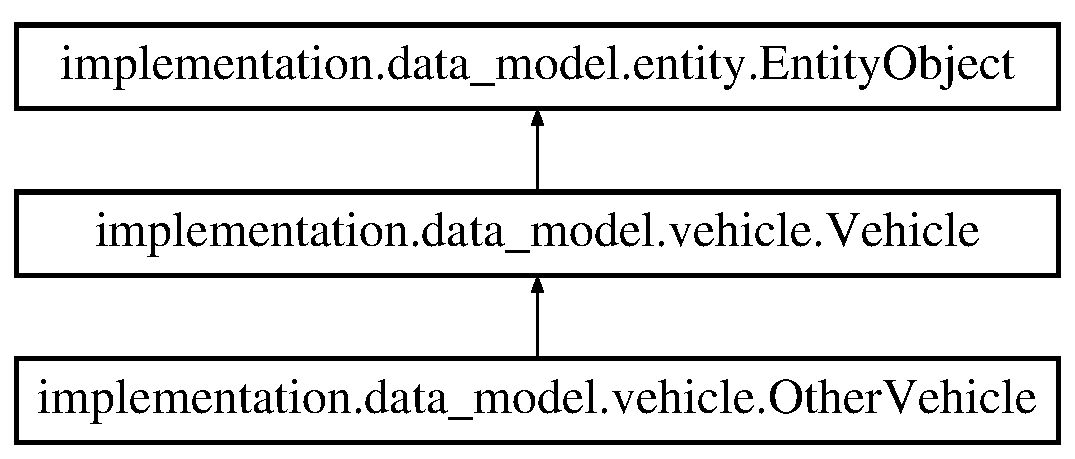
\includegraphics[height=3.000000cm]{classimplementation_1_1data__model_1_1vehicle_1_1_other_vehicle}
\end{center}
\end{figure}
\subsection*{Public Member Functions}
\begin{DoxyCompactItemize}
\item 
def \hyperlink{classimplementation_1_1data__model_1_1vehicle_1_1_other_vehicle_a9f8e9fb2fde253bf05b3b39c816b31bc}{\+\_\+\+\_\+hash\+\_\+\+\_\+} (self)
\end{DoxyCompactItemize}
\subsection*{Static Public Attributes}
\begin{DoxyCompactItemize}
\item 
\hyperlink{classimplementation_1_1data__model_1_1vehicle_1_1_other_vehicle_ab0196aae1ffc72e88df02cf3992efaaf}{int}
\item 
\hyperlink{classimplementation_1_1data__model_1_1vehicle_1_1_other_vehicle_aece2c603a961ed55846d522192ff63d2}{str}
\end{DoxyCompactItemize}


\subsection{Member Function Documentation}
\mbox{\Hypertarget{classimplementation_1_1data__model_1_1vehicle_1_1_other_vehicle_a9f8e9fb2fde253bf05b3b39c816b31bc}\label{classimplementation_1_1data__model_1_1vehicle_1_1_other_vehicle_a9f8e9fb2fde253bf05b3b39c816b31bc}} 
\index{implementation\+::data\+\_\+model\+::vehicle\+::\+Other\+Vehicle@{implementation\+::data\+\_\+model\+::vehicle\+::\+Other\+Vehicle}!\+\_\+\+\_\+hash\+\_\+\+\_\+@{\+\_\+\+\_\+hash\+\_\+\+\_\+}}
\index{\+\_\+\+\_\+hash\+\_\+\+\_\+@{\+\_\+\+\_\+hash\+\_\+\+\_\+}!implementation\+::data\+\_\+model\+::vehicle\+::\+Other\+Vehicle@{implementation\+::data\+\_\+model\+::vehicle\+::\+Other\+Vehicle}}
\subsubsection{\texorpdfstring{\+\_\+\+\_\+hash\+\_\+\+\_\+()}{\_\_hash\_\_()}}
{\footnotesize\ttfamily def implementation.\+data\+\_\+model.\+vehicle.\+Other\+Vehicle.\+\_\+\+\_\+hash\+\_\+\+\_\+ (\begin{DoxyParamCaption}\item[{}]{self }\end{DoxyParamCaption})}



\subsection{Member Data Documentation}
\mbox{\Hypertarget{classimplementation_1_1data__model_1_1vehicle_1_1_other_vehicle_ab0196aae1ffc72e88df02cf3992efaaf}\label{classimplementation_1_1data__model_1_1vehicle_1_1_other_vehicle_ab0196aae1ffc72e88df02cf3992efaaf}} 
\index{implementation\+::data\+\_\+model\+::vehicle\+::\+Other\+Vehicle@{implementation\+::data\+\_\+model\+::vehicle\+::\+Other\+Vehicle}!int@{int}}
\index{int@{int}!implementation\+::data\+\_\+model\+::vehicle\+::\+Other\+Vehicle@{implementation\+::data\+\_\+model\+::vehicle\+::\+Other\+Vehicle}}
\subsubsection{\texorpdfstring{int}{int}}
{\footnotesize\ttfamily implementation.\+data\+\_\+model.\+vehicle.\+Other\+Vehicle.\+int\hspace{0.3cm}{\ttfamily [static]}}

\mbox{\Hypertarget{classimplementation_1_1data__model_1_1vehicle_1_1_other_vehicle_aece2c603a961ed55846d522192ff63d2}\label{classimplementation_1_1data__model_1_1vehicle_1_1_other_vehicle_aece2c603a961ed55846d522192ff63d2}} 
\index{implementation\+::data\+\_\+model\+::vehicle\+::\+Other\+Vehicle@{implementation\+::data\+\_\+model\+::vehicle\+::\+Other\+Vehicle}!str@{str}}
\index{str@{str}!implementation\+::data\+\_\+model\+::vehicle\+::\+Other\+Vehicle@{implementation\+::data\+\_\+model\+::vehicle\+::\+Other\+Vehicle}}
\subsubsection{\texorpdfstring{str}{str}}
{\footnotesize\ttfamily implementation.\+data\+\_\+model.\+vehicle.\+Other\+Vehicle.\+str\hspace{0.3cm}{\ttfamily [static]}}



The documentation for this class was generated from the following file\+:\begin{DoxyCompactItemize}
\item 
implementation/data\+\_\+model/\hyperlink{vehicle_8py}{vehicle.\+py}\end{DoxyCompactItemize}

\hypertarget{classimplementation_1_1bayesian__network_1_1inference_1_1interfaces_1_1_outcome}{}\section{implementation.\+bayesian\+\_\+network.\+inference.\+interfaces.\+Outcome Class Reference}
\label{classimplementation_1_1bayesian__network_1_1inference_1_1interfaces_1_1_outcome}\index{implementation.\+bayesian\+\_\+network.\+inference.\+interfaces.\+Outcome@{implementation.\+bayesian\+\_\+network.\+inference.\+interfaces.\+Outcome}}


\subsection{Detailed Description}
\begin{DoxyVerb}Data class that describes a specific state with its value of a node in a Bayesian network.
(Python dataclasses.dataclass object.)

Attributes
----------
name : str
    Name of this specific state/outcome.
value : float
    Value/probability for this specific state/outcome.
\end{DoxyVerb}
 

The documentation for this class was generated from the following file\+:\begin{DoxyCompactItemize}
\item 
implementation/bayesian\+\_\+network/inference/\hyperlink{interfaces_8py}{interfaces.\+py}\end{DoxyCompactItemize}

\hypertarget{classimplementation_1_1data__model_1_1entity_1_1_pedestrian}{}\section{implementation.\+data\+\_\+model.\+entity.\+Pedestrian Class Reference}
\label{classimplementation_1_1data__model_1_1entity_1_1_pedestrian}\index{implementation.\+data\+\_\+model.\+entity.\+Pedestrian@{implementation.\+data\+\_\+model.\+entity.\+Pedestrian}}
Inheritance diagram for implementation.\+data\+\_\+model.\+entity.\+Pedestrian\+:\begin{figure}[H]
\begin{center}
\leavevmode
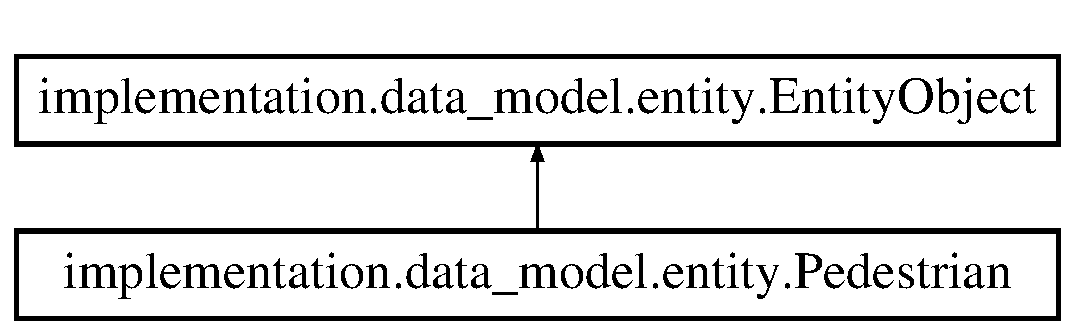
\includegraphics[height=2.000000cm]{classimplementation_1_1data__model_1_1entity_1_1_pedestrian}
\end{center}
\end{figure}
\subsection*{Static Public Attributes}
\begin{DoxyCompactItemize}
\item 
\hyperlink{classimplementation_1_1data__model_1_1entity_1_1_pedestrian_a32f375a8c021a43d5784348a15e232e9}{Pedestrian\+Category}
\end{DoxyCompactItemize}
\subsection*{Additional Inherited Members}


\subsection{Member Data Documentation}
\mbox{\Hypertarget{classimplementation_1_1data__model_1_1entity_1_1_pedestrian_a32f375a8c021a43d5784348a15e232e9}\label{classimplementation_1_1data__model_1_1entity_1_1_pedestrian_a32f375a8c021a43d5784348a15e232e9}} 
\index{implementation\+::data\+\_\+model\+::entity\+::\+Pedestrian@{implementation\+::data\+\_\+model\+::entity\+::\+Pedestrian}!Pedestrian\+Category@{Pedestrian\+Category}}
\index{Pedestrian\+Category@{Pedestrian\+Category}!implementation\+::data\+\_\+model\+::entity\+::\+Pedestrian@{implementation\+::data\+\_\+model\+::entity\+::\+Pedestrian}}
\subsubsection{\texorpdfstring{Pedestrian\+Category}{PedestrianCategory}}
{\footnotesize\ttfamily implementation.\+data\+\_\+model.\+entity.\+Pedestrian.\+Pedestrian\+Category\hspace{0.3cm}{\ttfamily [static]}}



The documentation for this class was generated from the following file\+:\begin{DoxyCompactItemize}
\item 
implementation/data\+\_\+model/\hyperlink{entity_8py}{entity.\+py}\end{DoxyCompactItemize}

\hypertarget{classimplementation_1_1data__model_1_1entity_1_1_pedestrian_category}{}\section{implementation.\+data\+\_\+model.\+entity.\+Pedestrian\+Category Class Reference}
\label{classimplementation_1_1data__model_1_1entity_1_1_pedestrian_category}\index{implementation.\+data\+\_\+model.\+entity.\+Pedestrian\+Category@{implementation.\+data\+\_\+model.\+entity.\+Pedestrian\+Category}}
Inheritance diagram for implementation.\+data\+\_\+model.\+entity.\+Pedestrian\+Category\+:\begin{figure}[H]
\begin{center}
\leavevmode
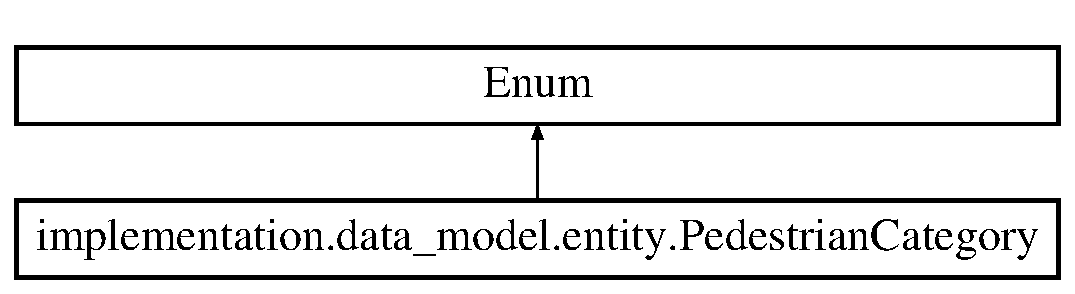
\includegraphics[height=2.000000cm]{classimplementation_1_1data__model_1_1entity_1_1_pedestrian_category}
\end{center}
\end{figure}
\subsection*{Static Public Attributes}
\begin{DoxyCompactItemize}
\item 
int \hyperlink{classimplementation_1_1data__model_1_1entity_1_1_pedestrian_category_a3a22fc8ad35d1437a3afe6097ee4d486}{P\+E\+D\+E\+S\+T\+R\+I\+AN} = 1
\item 
int \hyperlink{classimplementation_1_1data__model_1_1entity_1_1_pedestrian_category_a90e24b7d7df9a9d382e3b990181aaecd}{W\+H\+E\+E\+L\+C\+H\+A\+IR} = 2
\item 
int \hyperlink{classimplementation_1_1data__model_1_1entity_1_1_pedestrian_category_afab4565897518ef18eb5ce72526d96cb}{A\+N\+I\+M\+AL} = 3
\end{DoxyCompactItemize}


\subsection{Member Data Documentation}
\mbox{\Hypertarget{classimplementation_1_1data__model_1_1entity_1_1_pedestrian_category_afab4565897518ef18eb5ce72526d96cb}\label{classimplementation_1_1data__model_1_1entity_1_1_pedestrian_category_afab4565897518ef18eb5ce72526d96cb}} 
\index{implementation\+::data\+\_\+model\+::entity\+::\+Pedestrian\+Category@{implementation\+::data\+\_\+model\+::entity\+::\+Pedestrian\+Category}!A\+N\+I\+M\+AL@{A\+N\+I\+M\+AL}}
\index{A\+N\+I\+M\+AL@{A\+N\+I\+M\+AL}!implementation\+::data\+\_\+model\+::entity\+::\+Pedestrian\+Category@{implementation\+::data\+\_\+model\+::entity\+::\+Pedestrian\+Category}}
\subsubsection{\texorpdfstring{A\+N\+I\+M\+AL}{ANIMAL}}
{\footnotesize\ttfamily int implementation.\+data\+\_\+model.\+entity.\+Pedestrian\+Category.\+A\+N\+I\+M\+AL = 3\hspace{0.3cm}{\ttfamily [static]}}

\mbox{\Hypertarget{classimplementation_1_1data__model_1_1entity_1_1_pedestrian_category_a3a22fc8ad35d1437a3afe6097ee4d486}\label{classimplementation_1_1data__model_1_1entity_1_1_pedestrian_category_a3a22fc8ad35d1437a3afe6097ee4d486}} 
\index{implementation\+::data\+\_\+model\+::entity\+::\+Pedestrian\+Category@{implementation\+::data\+\_\+model\+::entity\+::\+Pedestrian\+Category}!P\+E\+D\+E\+S\+T\+R\+I\+AN@{P\+E\+D\+E\+S\+T\+R\+I\+AN}}
\index{P\+E\+D\+E\+S\+T\+R\+I\+AN@{P\+E\+D\+E\+S\+T\+R\+I\+AN}!implementation\+::data\+\_\+model\+::entity\+::\+Pedestrian\+Category@{implementation\+::data\+\_\+model\+::entity\+::\+Pedestrian\+Category}}
\subsubsection{\texorpdfstring{P\+E\+D\+E\+S\+T\+R\+I\+AN}{PEDESTRIAN}}
{\footnotesize\ttfamily int implementation.\+data\+\_\+model.\+entity.\+Pedestrian\+Category.\+P\+E\+D\+E\+S\+T\+R\+I\+AN = 1\hspace{0.3cm}{\ttfamily [static]}}

\mbox{\Hypertarget{classimplementation_1_1data__model_1_1entity_1_1_pedestrian_category_a90e24b7d7df9a9d382e3b990181aaecd}\label{classimplementation_1_1data__model_1_1entity_1_1_pedestrian_category_a90e24b7d7df9a9d382e3b990181aaecd}} 
\index{implementation\+::data\+\_\+model\+::entity\+::\+Pedestrian\+Category@{implementation\+::data\+\_\+model\+::entity\+::\+Pedestrian\+Category}!W\+H\+E\+E\+L\+C\+H\+A\+IR@{W\+H\+E\+E\+L\+C\+H\+A\+IR}}
\index{W\+H\+E\+E\+L\+C\+H\+A\+IR@{W\+H\+E\+E\+L\+C\+H\+A\+IR}!implementation\+::data\+\_\+model\+::entity\+::\+Pedestrian\+Category@{implementation\+::data\+\_\+model\+::entity\+::\+Pedestrian\+Category}}
\subsubsection{\texorpdfstring{W\+H\+E\+E\+L\+C\+H\+A\+IR}{WHEELCHAIR}}
{\footnotesize\ttfamily int implementation.\+data\+\_\+model.\+entity.\+Pedestrian\+Category.\+W\+H\+E\+E\+L\+C\+H\+A\+IR = 2\hspace{0.3cm}{\ttfamily [static]}}



The documentation for this class was generated from the following file\+:\begin{DoxyCompactItemize}
\item 
implementation/data\+\_\+model/\hyperlink{entity_8py}{entity.\+py}\end{DoxyCompactItemize}

\hypertarget{classimplementation_1_1data__model_1_1vehicle_1_1_performance}{}\section{implementation.\+data\+\_\+model.\+vehicle.\+Performance Class Reference}
\label{classimplementation_1_1data__model_1_1vehicle_1_1_performance}\index{implementation.\+data\+\_\+model.\+vehicle.\+Performance@{implementation.\+data\+\_\+model.\+vehicle.\+Performance}}


The documentation for this class was generated from the following file\+:\begin{DoxyCompactItemize}
\item 
implementation/data\+\_\+model/\hyperlink{vehicle_8py}{vehicle.\+py}\end{DoxyCompactItemize}

\hypertarget{classimplementation_1_1util_1_1kinematic__transform_1_1_pose}{}\doxysection{implementation.\+util.\+kinematic\+\_\+transform.\+Pose Class Reference}
\label{classimplementation_1_1util_1_1kinematic__transform_1_1_pose}\index{implementation.util.kinematic\_transform.Pose@{implementation.util.kinematic\_transform.Pose}}
\doxysubsection*{Static Public Attributes}
\begin{DoxyCompactItemize}
\item 
\mbox{\hyperlink{classimplementation_1_1util_1_1kinematic__transform_1_1_pose_afc2edf1ce8150514645a31bc242f5d2b}{float}}
\end{DoxyCompactItemize}


\doxysubsection{Member Data Documentation}
\mbox{\Hypertarget{classimplementation_1_1util_1_1kinematic__transform_1_1_pose_afc2edf1ce8150514645a31bc242f5d2b}\label{classimplementation_1_1util_1_1kinematic__transform_1_1_pose_afc2edf1ce8150514645a31bc242f5d2b}} 
\index{implementation.util.kinematic\_transform.Pose@{implementation.util.kinematic\_transform.Pose}!float@{float}}
\index{float@{float}!implementation.util.kinematic\_transform.Pose@{implementation.util.kinematic\_transform.Pose}}
\doxysubsubsection{\texorpdfstring{float}{float}}
{\footnotesize\ttfamily implementation.\+util.\+kinematic\+\_\+transform.\+Pose.\+float\hspace{0.3cm}{\ttfamily [static]}}



The documentation for this class was generated from the following file\+:\begin{DoxyCompactItemize}
\item 
implementation/util/\mbox{\hyperlink{kinematic__transform_8py}{kinematic\+\_\+transform.\+py}}\end{DoxyCompactItemize}

\hypertarget{classimplementation_1_1data__model_1_1positions_1_1_position}{}\section{implementation.\+data\+\_\+model.\+positions.\+Position Class Reference}
\label{classimplementation_1_1data__model_1_1positions_1_1_position}\index{implementation.\+data\+\_\+model.\+positions.\+Position@{implementation.\+data\+\_\+model.\+positions.\+Position}}
\subsection*{Static Public Attributes}
\begin{DoxyCompactItemize}
\item 
\hyperlink{classimplementation_1_1data__model_1_1positions_1_1_position_ab6bf0daf16f6e920f5066551359fbf09}{World\+Position}
\end{DoxyCompactItemize}


\subsection{Member Data Documentation}
\mbox{\Hypertarget{classimplementation_1_1data__model_1_1positions_1_1_position_ab6bf0daf16f6e920f5066551359fbf09}\label{classimplementation_1_1data__model_1_1positions_1_1_position_ab6bf0daf16f6e920f5066551359fbf09}} 
\index{implementation\+::data\+\_\+model\+::positions\+::\+Position@{implementation\+::data\+\_\+model\+::positions\+::\+Position}!World\+Position@{World\+Position}}
\index{World\+Position@{World\+Position}!implementation\+::data\+\_\+model\+::positions\+::\+Position@{implementation\+::data\+\_\+model\+::positions\+::\+Position}}
\subsubsection{\texorpdfstring{World\+Position}{WorldPosition}}
{\footnotesize\ttfamily implementation.\+data\+\_\+model.\+positions.\+Position.\+World\+Position\hspace{0.3cm}{\ttfamily [static]}}



The documentation for this class was generated from the following file\+:\begin{DoxyCompactItemize}
\item 
implementation/data\+\_\+model/\hyperlink{positions_8py}{positions.\+py}\end{DoxyCompactItemize}

\hypertarget{classimplementation_1_1data__model_1_1positions_1_1_position_in_lane_coordinates}{}\section{implementation.\+data\+\_\+model.\+positions.\+Position\+In\+Lane\+Coordinates Class Reference}
\label{classimplementation_1_1data__model_1_1positions_1_1_position_in_lane_coordinates}\index{implementation.\+data\+\_\+model.\+positions.\+Position\+In\+Lane\+Coordinates@{implementation.\+data\+\_\+model.\+positions.\+Position\+In\+Lane\+Coordinates}}
\subsection*{Static Public Attributes}
\begin{DoxyCompactItemize}
\item 
\hyperlink{classimplementation_1_1data__model_1_1positions_1_1_position_in_lane_coordinates_a0bc4ca4d3bd147f689e5690460da24ec}{str}
\item 
\hyperlink{classimplementation_1_1data__model_1_1positions_1_1_position_in_lane_coordinates_a3174976559286cff0d7ad21c3bccc495}{float}
\end{DoxyCompactItemize}


\subsection{Member Data Documentation}
\mbox{\Hypertarget{classimplementation_1_1data__model_1_1positions_1_1_position_in_lane_coordinates_a3174976559286cff0d7ad21c3bccc495}\label{classimplementation_1_1data__model_1_1positions_1_1_position_in_lane_coordinates_a3174976559286cff0d7ad21c3bccc495}} 
\index{implementation\+::data\+\_\+model\+::positions\+::\+Position\+In\+Lane\+Coordinates@{implementation\+::data\+\_\+model\+::positions\+::\+Position\+In\+Lane\+Coordinates}!float@{float}}
\index{float@{float}!implementation\+::data\+\_\+model\+::positions\+::\+Position\+In\+Lane\+Coordinates@{implementation\+::data\+\_\+model\+::positions\+::\+Position\+In\+Lane\+Coordinates}}
\subsubsection{\texorpdfstring{float}{float}}
{\footnotesize\ttfamily implementation.\+data\+\_\+model.\+positions.\+Position\+In\+Lane\+Coordinates.\+float\hspace{0.3cm}{\ttfamily [static]}}

\mbox{\Hypertarget{classimplementation_1_1data__model_1_1positions_1_1_position_in_lane_coordinates_a0bc4ca4d3bd147f689e5690460da24ec}\label{classimplementation_1_1data__model_1_1positions_1_1_position_in_lane_coordinates_a0bc4ca4d3bd147f689e5690460da24ec}} 
\index{implementation\+::data\+\_\+model\+::positions\+::\+Position\+In\+Lane\+Coordinates@{implementation\+::data\+\_\+model\+::positions\+::\+Position\+In\+Lane\+Coordinates}!str@{str}}
\index{str@{str}!implementation\+::data\+\_\+model\+::positions\+::\+Position\+In\+Lane\+Coordinates@{implementation\+::data\+\_\+model\+::positions\+::\+Position\+In\+Lane\+Coordinates}}
\subsubsection{\texorpdfstring{str}{str}}
{\footnotesize\ttfamily implementation.\+data\+\_\+model.\+positions.\+Position\+In\+Lane\+Coordinates.\+str\hspace{0.3cm}{\ttfamily [static]}}



The documentation for this class was generated from the following file\+:\begin{DoxyCompactItemize}
\item 
implementation/data\+\_\+model/\hyperlink{positions_8py}{positions.\+py}\end{DoxyCompactItemize}

\hypertarget{classimplementation_1_1data__model_1_1positions_1_1_position_in_road_coordinates}{}\section{implementation.\+data\+\_\+model.\+positions.\+Position\+In\+Road\+Coordinates Class Reference}
\label{classimplementation_1_1data__model_1_1positions_1_1_position_in_road_coordinates}\index{implementation.\+data\+\_\+model.\+positions.\+Position\+In\+Road\+Coordinates@{implementation.\+data\+\_\+model.\+positions.\+Position\+In\+Road\+Coordinates}}
\subsection*{Static Public Attributes}
\begin{DoxyCompactItemize}
\item 
\hyperlink{classimplementation_1_1data__model_1_1positions_1_1_position_in_road_coordinates_a2dde876c5460a82024fc340fd5000154}{float}
\end{DoxyCompactItemize}


\subsection{Member Data Documentation}
\mbox{\Hypertarget{classimplementation_1_1data__model_1_1positions_1_1_position_in_road_coordinates_a2dde876c5460a82024fc340fd5000154}\label{classimplementation_1_1data__model_1_1positions_1_1_position_in_road_coordinates_a2dde876c5460a82024fc340fd5000154}} 
\index{implementation\+::data\+\_\+model\+::positions\+::\+Position\+In\+Road\+Coordinates@{implementation\+::data\+\_\+model\+::positions\+::\+Position\+In\+Road\+Coordinates}!float@{float}}
\index{float@{float}!implementation\+::data\+\_\+model\+::positions\+::\+Position\+In\+Road\+Coordinates@{implementation\+::data\+\_\+model\+::positions\+::\+Position\+In\+Road\+Coordinates}}
\subsubsection{\texorpdfstring{float}{float}}
{\footnotesize\ttfamily implementation.\+data\+\_\+model.\+positions.\+Position\+In\+Road\+Coordinates.\+float\hspace{0.3cm}{\ttfamily [static]}}



The documentation for this class was generated from the following file\+:\begin{DoxyCompactItemize}
\item 
implementation/data\+\_\+model/\hyperlink{positions_8py}{positions.\+py}\end{DoxyCompactItemize}

\hypertarget{classimplementation_1_1data__model_1_1positions_1_1_position_of_current_entity}{}\section{implementation.\+data\+\_\+model.\+positions.\+Position\+Of\+Current\+Entity Class Reference}
\label{classimplementation_1_1data__model_1_1positions_1_1_position_of_current_entity}\index{implementation.\+data\+\_\+model.\+positions.\+Position\+Of\+Current\+Entity@{implementation.\+data\+\_\+model.\+positions.\+Position\+Of\+Current\+Entity}}


The documentation for this class was generated from the following file\+:\begin{DoxyCompactItemize}
\item 
implementation/data\+\_\+model/\hyperlink{positions_8py}{positions.\+py}\end{DoxyCompactItemize}

\hypertarget{classimplementation_1_1data__model_1_1environment_1_1_precipitation}{}\section{implementation.\+data\+\_\+model.\+environment.\+Precipitation Class Reference}
\label{classimplementation_1_1data__model_1_1environment_1_1_precipitation}\index{implementation.\+data\+\_\+model.\+environment.\+Precipitation@{implementation.\+data\+\_\+model.\+environment.\+Precipitation}}
\subsection*{Static Public Attributes}
\begin{DoxyCompactItemize}
\item 
\hyperlink{classimplementation_1_1data__model_1_1environment_1_1_precipitation_a610ff2eb19f9f26135dbc16afb852992}{float}
\end{DoxyCompactItemize}


\subsection{Member Data Documentation}
\mbox{\Hypertarget{classimplementation_1_1data__model_1_1environment_1_1_precipitation_a610ff2eb19f9f26135dbc16afb852992}\label{classimplementation_1_1data__model_1_1environment_1_1_precipitation_a610ff2eb19f9f26135dbc16afb852992}} 
\index{implementation\+::data\+\_\+model\+::environment\+::\+Precipitation@{implementation\+::data\+\_\+model\+::environment\+::\+Precipitation}!float@{float}}
\index{float@{float}!implementation\+::data\+\_\+model\+::environment\+::\+Precipitation@{implementation\+::data\+\_\+model\+::environment\+::\+Precipitation}}
\subsubsection{\texorpdfstring{float}{float}}
{\footnotesize\ttfamily implementation.\+data\+\_\+model.\+environment.\+Precipitation.\+float\hspace{0.3cm}{\ttfamily [static]}}



The documentation for this class was generated from the following file\+:\begin{DoxyCompactItemize}
\item 
implementation/data\+\_\+model/\hyperlink{environment_8py}{environment.\+py}\end{DoxyCompactItemize}

\hypertarget{classimplementation_1_1data__model_1_1environment_1_1_precipitation_type}{}\section{implementation.\+data\+\_\+model.\+environment.\+Precipitation\+Type Class Reference}
\label{classimplementation_1_1data__model_1_1environment_1_1_precipitation_type}\index{implementation.\+data\+\_\+model.\+environment.\+Precipitation\+Type@{implementation.\+data\+\_\+model.\+environment.\+Precipitation\+Type}}
Inheritance diagram for implementation.\+data\+\_\+model.\+environment.\+Precipitation\+Type\+:\begin{figure}[H]
\begin{center}
\leavevmode
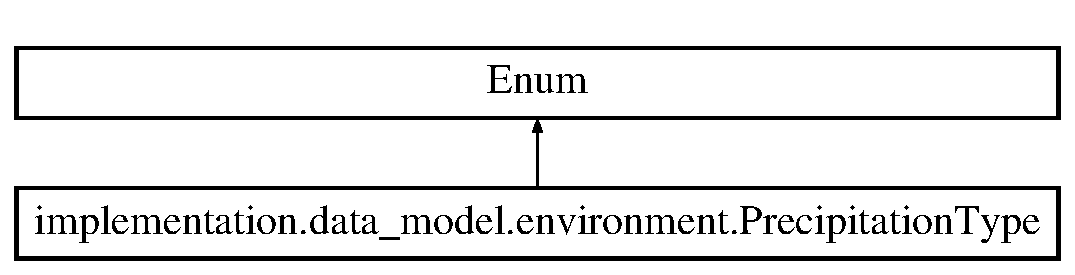
\includegraphics[height=2.000000cm]{classimplementation_1_1data__model_1_1environment_1_1_precipitation_type}
\end{center}
\end{figure}
\subsection*{Static Public Attributes}
\begin{DoxyCompactItemize}
\item 
int \hyperlink{classimplementation_1_1data__model_1_1environment_1_1_precipitation_type_aa14685436950d0d597c4ae4aadface46}{D\+RY} = 1
\item 
int \hyperlink{classimplementation_1_1data__model_1_1environment_1_1_precipitation_type_afcb84c05898e8352c797abc81ee5f4e3}{R\+A\+IN} = 2
\item 
int \hyperlink{classimplementation_1_1data__model_1_1environment_1_1_precipitation_type_ab4becec45f8343c5a423e8728a278cd0}{S\+N\+OW} = 3
\end{DoxyCompactItemize}


\subsection{Member Data Documentation}
\mbox{\Hypertarget{classimplementation_1_1data__model_1_1environment_1_1_precipitation_type_aa14685436950d0d597c4ae4aadface46}\label{classimplementation_1_1data__model_1_1environment_1_1_precipitation_type_aa14685436950d0d597c4ae4aadface46}} 
\index{implementation\+::data\+\_\+model\+::environment\+::\+Precipitation\+Type@{implementation\+::data\+\_\+model\+::environment\+::\+Precipitation\+Type}!D\+RY@{D\+RY}}
\index{D\+RY@{D\+RY}!implementation\+::data\+\_\+model\+::environment\+::\+Precipitation\+Type@{implementation\+::data\+\_\+model\+::environment\+::\+Precipitation\+Type}}
\subsubsection{\texorpdfstring{D\+RY}{DRY}}
{\footnotesize\ttfamily int implementation.\+data\+\_\+model.\+environment.\+Precipitation\+Type.\+D\+RY = 1\hspace{0.3cm}{\ttfamily [static]}}

\mbox{\Hypertarget{classimplementation_1_1data__model_1_1environment_1_1_precipitation_type_afcb84c05898e8352c797abc81ee5f4e3}\label{classimplementation_1_1data__model_1_1environment_1_1_precipitation_type_afcb84c05898e8352c797abc81ee5f4e3}} 
\index{implementation\+::data\+\_\+model\+::environment\+::\+Precipitation\+Type@{implementation\+::data\+\_\+model\+::environment\+::\+Precipitation\+Type}!R\+A\+IN@{R\+A\+IN}}
\index{R\+A\+IN@{R\+A\+IN}!implementation\+::data\+\_\+model\+::environment\+::\+Precipitation\+Type@{implementation\+::data\+\_\+model\+::environment\+::\+Precipitation\+Type}}
\subsubsection{\texorpdfstring{R\+A\+IN}{RAIN}}
{\footnotesize\ttfamily int implementation.\+data\+\_\+model.\+environment.\+Precipitation\+Type.\+R\+A\+IN = 2\hspace{0.3cm}{\ttfamily [static]}}

\mbox{\Hypertarget{classimplementation_1_1data__model_1_1environment_1_1_precipitation_type_ab4becec45f8343c5a423e8728a278cd0}\label{classimplementation_1_1data__model_1_1environment_1_1_precipitation_type_ab4becec45f8343c5a423e8728a278cd0}} 
\index{implementation\+::data\+\_\+model\+::environment\+::\+Precipitation\+Type@{implementation\+::data\+\_\+model\+::environment\+::\+Precipitation\+Type}!S\+N\+OW@{S\+N\+OW}}
\index{S\+N\+OW@{S\+N\+OW}!implementation\+::data\+\_\+model\+::environment\+::\+Precipitation\+Type@{implementation\+::data\+\_\+model\+::environment\+::\+Precipitation\+Type}}
\subsubsection{\texorpdfstring{S\+N\+OW}{SNOW}}
{\footnotesize\ttfamily int implementation.\+data\+\_\+model.\+environment.\+Precipitation\+Type.\+S\+N\+OW = 3\hspace{0.3cm}{\ttfamily [static]}}



The documentation for this class was generated from the following file\+:\begin{DoxyCompactItemize}
\item 
implementation/data\+\_\+model/\hyperlink{environment_8py}{environment.\+py}\end{DoxyCompactItemize}

\hypertarget{classimplementation_1_1manual__control_1_1_radar_sensor}{}\section{implementation.\+manual\+\_\+control.\+Radar\+Sensor Class Reference}
\label{classimplementation_1_1manual__control_1_1_radar_sensor}\index{implementation.\+manual\+\_\+control.\+Radar\+Sensor@{implementation.\+manual\+\_\+control.\+Radar\+Sensor}}
Inheritance diagram for implementation.\+manual\+\_\+control.\+Radar\+Sensor\+:\begin{figure}[H]
\begin{center}
\leavevmode
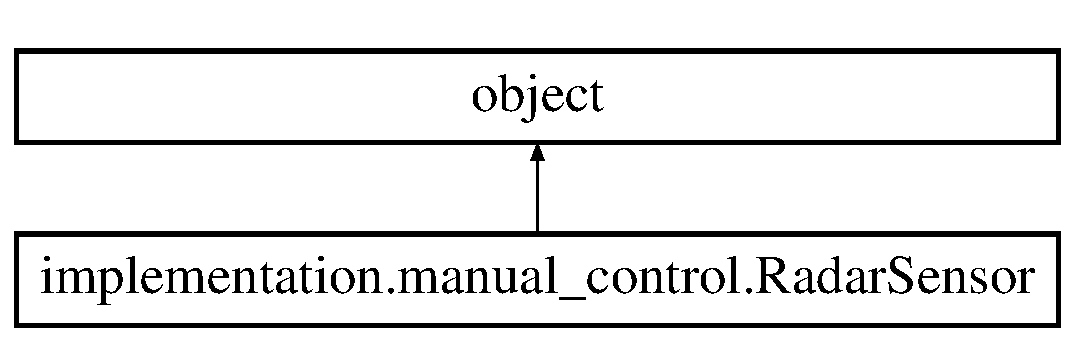
\includegraphics[height=2.000000cm]{classimplementation_1_1manual__control_1_1_radar_sensor}
\end{center}
\end{figure}
\subsection*{Public Member Functions}
\begin{DoxyCompactItemize}
\item 
def \hyperlink{classimplementation_1_1manual__control_1_1_radar_sensor_a89c9fcbfdbe0ca15c2095143b387affe}{\+\_\+\+\_\+init\+\_\+\+\_\+} (self, parent\+\_\+actor)
\end{DoxyCompactItemize}
\subsection*{Public Attributes}
\begin{DoxyCompactItemize}
\item 
\hyperlink{classimplementation_1_1manual__control_1_1_radar_sensor_a73fe61c634c78ea7673ee91521d61ab8}{sensor}
\item 
\hyperlink{classimplementation_1_1manual__control_1_1_radar_sensor_a049e3192b2bd3aa880858500f069992b}{velocity\+\_\+range}
\item 
\hyperlink{classimplementation_1_1manual__control_1_1_radar_sensor_a3dd1cefeb96ddc248a5e729532b516ad}{debug}
\end{DoxyCompactItemize}


\subsection{Constructor \& Destructor Documentation}
\mbox{\Hypertarget{classimplementation_1_1manual__control_1_1_radar_sensor_a89c9fcbfdbe0ca15c2095143b387affe}\label{classimplementation_1_1manual__control_1_1_radar_sensor_a89c9fcbfdbe0ca15c2095143b387affe}} 
\index{implementation\+::manual\+\_\+control\+::\+Radar\+Sensor@{implementation\+::manual\+\_\+control\+::\+Radar\+Sensor}!\+\_\+\+\_\+init\+\_\+\+\_\+@{\+\_\+\+\_\+init\+\_\+\+\_\+}}
\index{\+\_\+\+\_\+init\+\_\+\+\_\+@{\+\_\+\+\_\+init\+\_\+\+\_\+}!implementation\+::manual\+\_\+control\+::\+Radar\+Sensor@{implementation\+::manual\+\_\+control\+::\+Radar\+Sensor}}
\subsubsection{\texorpdfstring{\+\_\+\+\_\+init\+\_\+\+\_\+()}{\_\_init\_\_()}}
{\footnotesize\ttfamily def implementation.\+manual\+\_\+control.\+Radar\+Sensor.\+\_\+\+\_\+init\+\_\+\+\_\+ (\begin{DoxyParamCaption}\item[{}]{self,  }\item[{}]{parent\+\_\+actor }\end{DoxyParamCaption})}



\subsection{Member Data Documentation}
\mbox{\Hypertarget{classimplementation_1_1manual__control_1_1_radar_sensor_a3dd1cefeb96ddc248a5e729532b516ad}\label{classimplementation_1_1manual__control_1_1_radar_sensor_a3dd1cefeb96ddc248a5e729532b516ad}} 
\index{implementation\+::manual\+\_\+control\+::\+Radar\+Sensor@{implementation\+::manual\+\_\+control\+::\+Radar\+Sensor}!debug@{debug}}
\index{debug@{debug}!implementation\+::manual\+\_\+control\+::\+Radar\+Sensor@{implementation\+::manual\+\_\+control\+::\+Radar\+Sensor}}
\subsubsection{\texorpdfstring{debug}{debug}}
{\footnotesize\ttfamily implementation.\+manual\+\_\+control.\+Radar\+Sensor.\+debug}

\mbox{\Hypertarget{classimplementation_1_1manual__control_1_1_radar_sensor_a73fe61c634c78ea7673ee91521d61ab8}\label{classimplementation_1_1manual__control_1_1_radar_sensor_a73fe61c634c78ea7673ee91521d61ab8}} 
\index{implementation\+::manual\+\_\+control\+::\+Radar\+Sensor@{implementation\+::manual\+\_\+control\+::\+Radar\+Sensor}!sensor@{sensor}}
\index{sensor@{sensor}!implementation\+::manual\+\_\+control\+::\+Radar\+Sensor@{implementation\+::manual\+\_\+control\+::\+Radar\+Sensor}}
\subsubsection{\texorpdfstring{sensor}{sensor}}
{\footnotesize\ttfamily implementation.\+manual\+\_\+control.\+Radar\+Sensor.\+sensor}

\mbox{\Hypertarget{classimplementation_1_1manual__control_1_1_radar_sensor_a049e3192b2bd3aa880858500f069992b}\label{classimplementation_1_1manual__control_1_1_radar_sensor_a049e3192b2bd3aa880858500f069992b}} 
\index{implementation\+::manual\+\_\+control\+::\+Radar\+Sensor@{implementation\+::manual\+\_\+control\+::\+Radar\+Sensor}!velocity\+\_\+range@{velocity\+\_\+range}}
\index{velocity\+\_\+range@{velocity\+\_\+range}!implementation\+::manual\+\_\+control\+::\+Radar\+Sensor@{implementation\+::manual\+\_\+control\+::\+Radar\+Sensor}}
\subsubsection{\texorpdfstring{velocity\+\_\+range}{velocity\_range}}
{\footnotesize\ttfamily implementation.\+manual\+\_\+control.\+Radar\+Sensor.\+velocity\+\_\+range}



The documentation for this class was generated from the following file\+:\begin{DoxyCompactItemize}
\item 
implementation/\hyperlink{manual__control_8py}{manual\+\_\+control.\+py}\end{DoxyCompactItemize}

\hypertarget{classimplementation_1_1data__model_1_1positions_1_1_reference_context}{}\section{implementation.\+data\+\_\+model.\+positions.\+Reference\+Context Class Reference}
\label{classimplementation_1_1data__model_1_1positions_1_1_reference_context}\index{implementation.\+data\+\_\+model.\+positions.\+Reference\+Context@{implementation.\+data\+\_\+model.\+positions.\+Reference\+Context}}
Inheritance diagram for implementation.\+data\+\_\+model.\+positions.\+Reference\+Context\+:\begin{figure}[H]
\begin{center}
\leavevmode
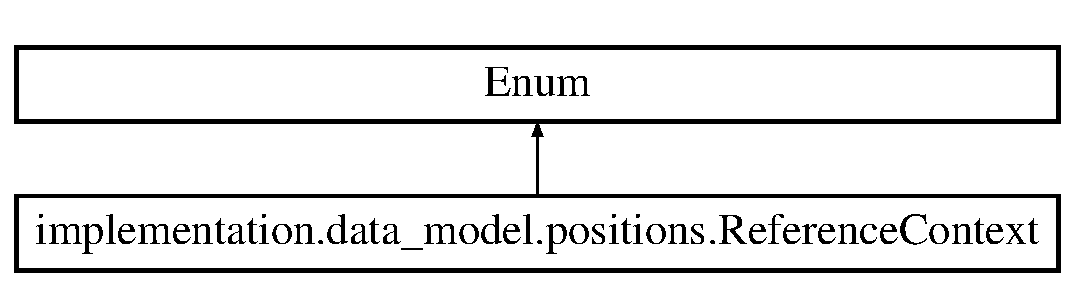
\includegraphics[height=2.000000cm]{classimplementation_1_1data__model_1_1positions_1_1_reference_context}
\end{center}
\end{figure}
\subsection*{Static Public Attributes}
\begin{DoxyCompactItemize}
\item 
int \hyperlink{classimplementation_1_1data__model_1_1positions_1_1_reference_context_ab0986ecf93ba929730d3d423efead9a3}{A\+B\+S\+O\+L\+U\+TE} = 1
\item 
int \hyperlink{classimplementation_1_1data__model_1_1positions_1_1_reference_context_a5c7cbdfc4022cc8021d12add9213111f}{R\+E\+L\+A\+T\+I\+VE} = 2
\end{DoxyCompactItemize}


\subsection{Member Data Documentation}
\mbox{\Hypertarget{classimplementation_1_1data__model_1_1positions_1_1_reference_context_ab0986ecf93ba929730d3d423efead9a3}\label{classimplementation_1_1data__model_1_1positions_1_1_reference_context_ab0986ecf93ba929730d3d423efead9a3}} 
\index{implementation\+::data\+\_\+model\+::positions\+::\+Reference\+Context@{implementation\+::data\+\_\+model\+::positions\+::\+Reference\+Context}!A\+B\+S\+O\+L\+U\+TE@{A\+B\+S\+O\+L\+U\+TE}}
\index{A\+B\+S\+O\+L\+U\+TE@{A\+B\+S\+O\+L\+U\+TE}!implementation\+::data\+\_\+model\+::positions\+::\+Reference\+Context@{implementation\+::data\+\_\+model\+::positions\+::\+Reference\+Context}}
\subsubsection{\texorpdfstring{A\+B\+S\+O\+L\+U\+TE}{ABSOLUTE}}
{\footnotesize\ttfamily int implementation.\+data\+\_\+model.\+positions.\+Reference\+Context.\+A\+B\+S\+O\+L\+U\+TE = 1\hspace{0.3cm}{\ttfamily [static]}}

\mbox{\Hypertarget{classimplementation_1_1data__model_1_1positions_1_1_reference_context_a5c7cbdfc4022cc8021d12add9213111f}\label{classimplementation_1_1data__model_1_1positions_1_1_reference_context_a5c7cbdfc4022cc8021d12add9213111f}} 
\index{implementation\+::data\+\_\+model\+::positions\+::\+Reference\+Context@{implementation\+::data\+\_\+model\+::positions\+::\+Reference\+Context}!R\+E\+L\+A\+T\+I\+VE@{R\+E\+L\+A\+T\+I\+VE}}
\index{R\+E\+L\+A\+T\+I\+VE@{R\+E\+L\+A\+T\+I\+VE}!implementation\+::data\+\_\+model\+::positions\+::\+Reference\+Context@{implementation\+::data\+\_\+model\+::positions\+::\+Reference\+Context}}
\subsubsection{\texorpdfstring{R\+E\+L\+A\+T\+I\+VE}{RELATIVE}}
{\footnotesize\ttfamily int implementation.\+data\+\_\+model.\+positions.\+Reference\+Context.\+R\+E\+L\+A\+T\+I\+VE = 2\hspace{0.3cm}{\ttfamily [static]}}



The documentation for this class was generated from the following file\+:\begin{DoxyCompactItemize}
\item 
implementation/data\+\_\+model/\hyperlink{positions_8py}{positions.\+py}\end{DoxyCompactItemize}

\hypertarget{classimplementation_1_1data__model_1_1positions_1_1_relative_lane_position}{}\section{implementation.\+data\+\_\+model.\+positions.\+Relative\+Lane\+Position Class Reference}
\label{classimplementation_1_1data__model_1_1positions_1_1_relative_lane_position}\index{implementation.\+data\+\_\+model.\+positions.\+Relative\+Lane\+Position@{implementation.\+data\+\_\+model.\+positions.\+Relative\+Lane\+Position}}
\subsection*{Static Public Attributes}
\begin{DoxyCompactItemize}
\item 
\hyperlink{classimplementation_1_1data__model_1_1positions_1_1_relative_lane_position_a44fb19dd037d4b1743a7d3ebf7ff07ef}{int}
\item 
\hyperlink{classimplementation_1_1data__model_1_1positions_1_1_relative_lane_position_a63129d10d9e66572aee5771ea13047db}{float}
\item 
\hyperlink{classimplementation_1_1data__model_1_1positions_1_1_relative_lane_position_a7ee3505d5a706ac45044054563a7477e}{Orientation}
\end{DoxyCompactItemize}


\subsection{Member Data Documentation}
\mbox{\Hypertarget{classimplementation_1_1data__model_1_1positions_1_1_relative_lane_position_a63129d10d9e66572aee5771ea13047db}\label{classimplementation_1_1data__model_1_1positions_1_1_relative_lane_position_a63129d10d9e66572aee5771ea13047db}} 
\index{implementation\+::data\+\_\+model\+::positions\+::\+Relative\+Lane\+Position@{implementation\+::data\+\_\+model\+::positions\+::\+Relative\+Lane\+Position}!float@{float}}
\index{float@{float}!implementation\+::data\+\_\+model\+::positions\+::\+Relative\+Lane\+Position@{implementation\+::data\+\_\+model\+::positions\+::\+Relative\+Lane\+Position}}
\subsubsection{\texorpdfstring{float}{float}}
{\footnotesize\ttfamily implementation.\+data\+\_\+model.\+positions.\+Relative\+Lane\+Position.\+float\hspace{0.3cm}{\ttfamily [static]}}

\mbox{\Hypertarget{classimplementation_1_1data__model_1_1positions_1_1_relative_lane_position_a44fb19dd037d4b1743a7d3ebf7ff07ef}\label{classimplementation_1_1data__model_1_1positions_1_1_relative_lane_position_a44fb19dd037d4b1743a7d3ebf7ff07ef}} 
\index{implementation\+::data\+\_\+model\+::positions\+::\+Relative\+Lane\+Position@{implementation\+::data\+\_\+model\+::positions\+::\+Relative\+Lane\+Position}!int@{int}}
\index{int@{int}!implementation\+::data\+\_\+model\+::positions\+::\+Relative\+Lane\+Position@{implementation\+::data\+\_\+model\+::positions\+::\+Relative\+Lane\+Position}}
\subsubsection{\texorpdfstring{int}{int}}
{\footnotesize\ttfamily implementation.\+data\+\_\+model.\+positions.\+Relative\+Lane\+Position.\+int\hspace{0.3cm}{\ttfamily [static]}}

\mbox{\Hypertarget{classimplementation_1_1data__model_1_1positions_1_1_relative_lane_position_a7ee3505d5a706ac45044054563a7477e}\label{classimplementation_1_1data__model_1_1positions_1_1_relative_lane_position_a7ee3505d5a706ac45044054563a7477e}} 
\index{implementation\+::data\+\_\+model\+::positions\+::\+Relative\+Lane\+Position@{implementation\+::data\+\_\+model\+::positions\+::\+Relative\+Lane\+Position}!Orientation@{Orientation}}
\index{Orientation@{Orientation}!implementation\+::data\+\_\+model\+::positions\+::\+Relative\+Lane\+Position@{implementation\+::data\+\_\+model\+::positions\+::\+Relative\+Lane\+Position}}
\subsubsection{\texorpdfstring{Orientation}{Orientation}}
{\footnotesize\ttfamily implementation.\+data\+\_\+model.\+positions.\+Relative\+Lane\+Position.\+Orientation\hspace{0.3cm}{\ttfamily [static]}}



The documentation for this class was generated from the following file\+:\begin{DoxyCompactItemize}
\item 
implementation/data\+\_\+model/\hyperlink{positions_8py}{positions.\+py}\end{DoxyCompactItemize}

\hypertarget{classimplementation_1_1data__model_1_1positions_1_1_relative_object_position}{}\section{implementation.\+data\+\_\+model.\+positions.\+Relative\+Object\+Position Class Reference}
\label{classimplementation_1_1data__model_1_1positions_1_1_relative_object_position}\index{implementation.\+data\+\_\+model.\+positions.\+Relative\+Object\+Position@{implementation.\+data\+\_\+model.\+positions.\+Relative\+Object\+Position}}
\subsection*{Static Public Attributes}
\begin{DoxyCompactItemize}
\item 
\hyperlink{classimplementation_1_1data__model_1_1positions_1_1_relative_object_position_a98cb7fca58fc77416cbc30921a6fb22f}{float}
\item 
\hyperlink{classimplementation_1_1data__model_1_1positions_1_1_relative_object_position_ac2bdd50b9aac336884d2c110eb8d9e4b}{Orientation}
\end{DoxyCompactItemize}


\subsection{Member Data Documentation}
\mbox{\Hypertarget{classimplementation_1_1data__model_1_1positions_1_1_relative_object_position_a98cb7fca58fc77416cbc30921a6fb22f}\label{classimplementation_1_1data__model_1_1positions_1_1_relative_object_position_a98cb7fca58fc77416cbc30921a6fb22f}} 
\index{implementation\+::data\+\_\+model\+::positions\+::\+Relative\+Object\+Position@{implementation\+::data\+\_\+model\+::positions\+::\+Relative\+Object\+Position}!float@{float}}
\index{float@{float}!implementation\+::data\+\_\+model\+::positions\+::\+Relative\+Object\+Position@{implementation\+::data\+\_\+model\+::positions\+::\+Relative\+Object\+Position}}
\subsubsection{\texorpdfstring{float}{float}}
{\footnotesize\ttfamily implementation.\+data\+\_\+model.\+positions.\+Relative\+Object\+Position.\+float\hspace{0.3cm}{\ttfamily [static]}}

\mbox{\Hypertarget{classimplementation_1_1data__model_1_1positions_1_1_relative_object_position_ac2bdd50b9aac336884d2c110eb8d9e4b}\label{classimplementation_1_1data__model_1_1positions_1_1_relative_object_position_ac2bdd50b9aac336884d2c110eb8d9e4b}} 
\index{implementation\+::data\+\_\+model\+::positions\+::\+Relative\+Object\+Position@{implementation\+::data\+\_\+model\+::positions\+::\+Relative\+Object\+Position}!Orientation@{Orientation}}
\index{Orientation@{Orientation}!implementation\+::data\+\_\+model\+::positions\+::\+Relative\+Object\+Position@{implementation\+::data\+\_\+model\+::positions\+::\+Relative\+Object\+Position}}
\subsubsection{\texorpdfstring{Orientation}{Orientation}}
{\footnotesize\ttfamily implementation.\+data\+\_\+model.\+positions.\+Relative\+Object\+Position.\+Orientation\hspace{0.3cm}{\ttfamily [static]}}



The documentation for this class was generated from the following file\+:\begin{DoxyCompactItemize}
\item 
implementation/data\+\_\+model/\hyperlink{positions_8py}{positions.\+py}\end{DoxyCompactItemize}

\hypertarget{classimplementation_1_1data__model_1_1positions_1_1_relative_road_position}{}\section{implementation.\+data\+\_\+model.\+positions.\+Relative\+Road\+Position Class Reference}
\label{classimplementation_1_1data__model_1_1positions_1_1_relative_road_position}\index{implementation.\+data\+\_\+model.\+positions.\+Relative\+Road\+Position@{implementation.\+data\+\_\+model.\+positions.\+Relative\+Road\+Position}}
\subsection*{Static Public Attributes}
\begin{DoxyCompactItemize}
\item 
\hyperlink{classimplementation_1_1data__model_1_1positions_1_1_relative_road_position_a50d99a47b7616a2bc12f656a26cd313f}{float}
\item 
\hyperlink{classimplementation_1_1data__model_1_1positions_1_1_relative_road_position_a4e4d32630a22a2a9a40487dac3ee0887}{Orientation}
\end{DoxyCompactItemize}


\subsection{Member Data Documentation}
\mbox{\Hypertarget{classimplementation_1_1data__model_1_1positions_1_1_relative_road_position_a50d99a47b7616a2bc12f656a26cd313f}\label{classimplementation_1_1data__model_1_1positions_1_1_relative_road_position_a50d99a47b7616a2bc12f656a26cd313f}} 
\index{implementation\+::data\+\_\+model\+::positions\+::\+Relative\+Road\+Position@{implementation\+::data\+\_\+model\+::positions\+::\+Relative\+Road\+Position}!float@{float}}
\index{float@{float}!implementation\+::data\+\_\+model\+::positions\+::\+Relative\+Road\+Position@{implementation\+::data\+\_\+model\+::positions\+::\+Relative\+Road\+Position}}
\subsubsection{\texorpdfstring{float}{float}}
{\footnotesize\ttfamily implementation.\+data\+\_\+model.\+positions.\+Relative\+Road\+Position.\+float\hspace{0.3cm}{\ttfamily [static]}}

\mbox{\Hypertarget{classimplementation_1_1data__model_1_1positions_1_1_relative_road_position_a4e4d32630a22a2a9a40487dac3ee0887}\label{classimplementation_1_1data__model_1_1positions_1_1_relative_road_position_a4e4d32630a22a2a9a40487dac3ee0887}} 
\index{implementation\+::data\+\_\+model\+::positions\+::\+Relative\+Road\+Position@{implementation\+::data\+\_\+model\+::positions\+::\+Relative\+Road\+Position}!Orientation@{Orientation}}
\index{Orientation@{Orientation}!implementation\+::data\+\_\+model\+::positions\+::\+Relative\+Road\+Position@{implementation\+::data\+\_\+model\+::positions\+::\+Relative\+Road\+Position}}
\subsubsection{\texorpdfstring{Orientation}{Orientation}}
{\footnotesize\ttfamily implementation.\+data\+\_\+model.\+positions.\+Relative\+Road\+Position.\+Orientation\hspace{0.3cm}{\ttfamily [static]}}



The documentation for this class was generated from the following file\+:\begin{DoxyCompactItemize}
\item 
implementation/data\+\_\+model/\hyperlink{positions_8py}{positions.\+py}\end{DoxyCompactItemize}

\hypertarget{classimplementation_1_1data__model_1_1positions_1_1_relative_world_position}{}\section{implementation.\+data\+\_\+model.\+positions.\+Relative\+World\+Position Class Reference}
\label{classimplementation_1_1data__model_1_1positions_1_1_relative_world_position}\index{implementation.\+data\+\_\+model.\+positions.\+Relative\+World\+Position@{implementation.\+data\+\_\+model.\+positions.\+Relative\+World\+Position}}
\subsection*{Static Public Attributes}
\begin{DoxyCompactItemize}
\item 
\hyperlink{classimplementation_1_1data__model_1_1positions_1_1_relative_world_position_a0d0ff0796894412ab275b1ecd5d320dc}{float}
\item 
\hyperlink{classimplementation_1_1data__model_1_1positions_1_1_relative_world_position_a44640b0d5dc5b4a56da948f291086c2a}{Orientation}
\end{DoxyCompactItemize}


\subsection{Member Data Documentation}
\mbox{\Hypertarget{classimplementation_1_1data__model_1_1positions_1_1_relative_world_position_a0d0ff0796894412ab275b1ecd5d320dc}\label{classimplementation_1_1data__model_1_1positions_1_1_relative_world_position_a0d0ff0796894412ab275b1ecd5d320dc}} 
\index{implementation\+::data\+\_\+model\+::positions\+::\+Relative\+World\+Position@{implementation\+::data\+\_\+model\+::positions\+::\+Relative\+World\+Position}!float@{float}}
\index{float@{float}!implementation\+::data\+\_\+model\+::positions\+::\+Relative\+World\+Position@{implementation\+::data\+\_\+model\+::positions\+::\+Relative\+World\+Position}}
\subsubsection{\texorpdfstring{float}{float}}
{\footnotesize\ttfamily implementation.\+data\+\_\+model.\+positions.\+Relative\+World\+Position.\+float\hspace{0.3cm}{\ttfamily [static]}}

\mbox{\Hypertarget{classimplementation_1_1data__model_1_1positions_1_1_relative_world_position_a44640b0d5dc5b4a56da948f291086c2a}\label{classimplementation_1_1data__model_1_1positions_1_1_relative_world_position_a44640b0d5dc5b4a56da948f291086c2a}} 
\index{implementation\+::data\+\_\+model\+::positions\+::\+Relative\+World\+Position@{implementation\+::data\+\_\+model\+::positions\+::\+Relative\+World\+Position}!Orientation@{Orientation}}
\index{Orientation@{Orientation}!implementation\+::data\+\_\+model\+::positions\+::\+Relative\+World\+Position@{implementation\+::data\+\_\+model\+::positions\+::\+Relative\+World\+Position}}
\subsubsection{\texorpdfstring{Orientation}{Orientation}}
{\footnotesize\ttfamily implementation.\+data\+\_\+model.\+positions.\+Relative\+World\+Position.\+Orientation\hspace{0.3cm}{\ttfamily [static]}}



The documentation for this class was generated from the following file\+:\begin{DoxyCompactItemize}
\item 
implementation/data\+\_\+model/\hyperlink{positions_8py}{positions.\+py}\end{DoxyCompactItemize}

\hypertarget{classimplementation_1_1util_1_1risk__plot_1_1_risk_plot}{}\section{implementation.\+util.\+risk\+\_\+plot.\+Risk\+Plot Class Reference}
\label{classimplementation_1_1util_1_1risk__plot_1_1_risk_plot}\index{implementation.\+util.\+risk\+\_\+plot.\+Risk\+Plot@{implementation.\+util.\+risk\+\_\+plot.\+Risk\+Plot}}
\subsection*{Public Member Functions}
\begin{DoxyCompactItemize}
\item 
def \hyperlink{classimplementation_1_1util_1_1risk__plot_1_1_risk_plot_a574b3dc33ab0b1859a5167eed072a321}{\+\_\+\+\_\+init\+\_\+\+\_\+} (self)
\item 
def \hyperlink{classimplementation_1_1util_1_1risk__plot_1_1_risk_plot_aea7addcd83af1bfe853a79490b834f02}{update\+\_\+and\+\_\+draw\+\_\+risk\+\_\+plot} (self)
\item 
def \hyperlink{classimplementation_1_1util_1_1risk__plot_1_1_risk_plot_a7055e0167a4c656e1b76a1363c1941af}{get\+\_\+rgb\+\_\+image} (self)
\item 
def \hyperlink{classimplementation_1_1util_1_1risk__plot_1_1_risk_plot_a10abb3130925f46b34d1cdb5cf3daf72}{get\+\_\+width\+\_\+height} (self)
\item 
def \hyperlink{classimplementation_1_1util_1_1risk__plot_1_1_risk_plot_ae1c12efeca8a144da4c4c67bcee20a42}{set\+\_\+front\+\_\+vehicle\+\_\+cumulative\+\_\+risk}
\item 
def \hyperlink{classimplementation_1_1util_1_1risk__plot_1_1_risk_plot_afff8dae32aa6e615595db6168671c167}{set\+\_\+front\+\_\+vehicle\+\_\+emergency\+\_\+risk}
\item 
def \hyperlink{classimplementation_1_1util_1_1risk__plot_1_1_risk_plot_a3ec57dafb9fc0f298105bd6170a6bd41}{set\+\_\+front\+\_\+vehicle\+\_\+target\+\_\+brake\+\_\+risk}
\item 
def \hyperlink{classimplementation_1_1util_1_1risk__plot_1_1_risk_plot_a4a13fbf2134f7ac6e093fd13f22db9cf}{set\+\_\+front\+\_\+vehicle\+\_\+idm\+\_\+risk}
\item 
def \hyperlink{classimplementation_1_1util_1_1risk__plot_1_1_risk_plot_a25770f1dbc983398d3a10350ba9d78e2}{set\+\_\+left\+\_\+side\+\_\+vehicle\+\_\+longitudinal\+\_\+risk}
\item 
def \hyperlink{classimplementation_1_1util_1_1risk__plot_1_1_risk_plot_a526e53adb44b439d39ad56f01b433b4b}{set\+\_\+left\+\_\+side\+\_\+vehicle\+\_\+lateral\+\_\+risk}
\item 
def \hyperlink{classimplementation_1_1util_1_1risk__plot_1_1_risk_plot_ae509278a9de364e6626c1ae12c80084f}{set\+\_\+right\+\_\+side\+\_\+vehicle\+\_\+longitudinal\+\_\+risk}
\item 
def \hyperlink{classimplementation_1_1util_1_1risk__plot_1_1_risk_plot_a80e5957e1f16e86a9c19e0b89777c286}{set\+\_\+right\+\_\+side\+\_\+vehicle\+\_\+lateral\+\_\+risk}
\item 
def \hyperlink{classimplementation_1_1util_1_1risk__plot_1_1_risk_plot_afa07c0b2874bbad1b3e98756f20e5d31}{save\+\_\+risk\+\_\+plot\+\_\+on\+\_\+disk}
\end{DoxyCompactItemize}


\subsection{Constructor \& Destructor Documentation}
\mbox{\Hypertarget{classimplementation_1_1util_1_1risk__plot_1_1_risk_plot_a574b3dc33ab0b1859a5167eed072a321}\label{classimplementation_1_1util_1_1risk__plot_1_1_risk_plot_a574b3dc33ab0b1859a5167eed072a321}} 
\index{implementation\+::util\+::risk\+\_\+plot\+::\+Risk\+Plot@{implementation\+::util\+::risk\+\_\+plot\+::\+Risk\+Plot}!\+\_\+\+\_\+init\+\_\+\+\_\+@{\+\_\+\+\_\+init\+\_\+\+\_\+}}
\index{\+\_\+\+\_\+init\+\_\+\+\_\+@{\+\_\+\+\_\+init\+\_\+\+\_\+}!implementation\+::util\+::risk\+\_\+plot\+::\+Risk\+Plot@{implementation\+::util\+::risk\+\_\+plot\+::\+Risk\+Plot}}
\subsubsection{\texorpdfstring{\+\_\+\+\_\+init\+\_\+\+\_\+()}{\_\_init\_\_()}}
{\footnotesize\ttfamily def implementation.\+util.\+risk\+\_\+plot.\+Risk\+Plot.\+\_\+\+\_\+init\+\_\+\+\_\+ (\begin{DoxyParamCaption}\item[{}]{self,  }\item[{}]{None }\end{DoxyParamCaption})}



\subsection{Member Function Documentation}
\mbox{\Hypertarget{classimplementation_1_1util_1_1risk__plot_1_1_risk_plot_a7055e0167a4c656e1b76a1363c1941af}\label{classimplementation_1_1util_1_1risk__plot_1_1_risk_plot_a7055e0167a4c656e1b76a1363c1941af}} 
\index{implementation\+::util\+::risk\+\_\+plot\+::\+Risk\+Plot@{implementation\+::util\+::risk\+\_\+plot\+::\+Risk\+Plot}!get\+\_\+rgb\+\_\+image@{get\+\_\+rgb\+\_\+image}}
\index{get\+\_\+rgb\+\_\+image@{get\+\_\+rgb\+\_\+image}!implementation\+::util\+::risk\+\_\+plot\+::\+Risk\+Plot@{implementation\+::util\+::risk\+\_\+plot\+::\+Risk\+Plot}}
\subsubsection{\texorpdfstring{get\+\_\+rgb\+\_\+image()}{get\_rgb\_image()}}
{\footnotesize\ttfamily def implementation.\+util.\+risk\+\_\+plot.\+Risk\+Plot.\+get\+\_\+rgb\+\_\+image (\begin{DoxyParamCaption}\item[{}]{self,  }\item[{}]{bytes }\end{DoxyParamCaption})}

\mbox{\Hypertarget{classimplementation_1_1util_1_1risk__plot_1_1_risk_plot_a10abb3130925f46b34d1cdb5cf3daf72}\label{classimplementation_1_1util_1_1risk__plot_1_1_risk_plot_a10abb3130925f46b34d1cdb5cf3daf72}} 
\index{implementation\+::util\+::risk\+\_\+plot\+::\+Risk\+Plot@{implementation\+::util\+::risk\+\_\+plot\+::\+Risk\+Plot}!get\+\_\+width\+\_\+height@{get\+\_\+width\+\_\+height}}
\index{get\+\_\+width\+\_\+height@{get\+\_\+width\+\_\+height}!implementation\+::util\+::risk\+\_\+plot\+::\+Risk\+Plot@{implementation\+::util\+::risk\+\_\+plot\+::\+Risk\+Plot}}
\subsubsection{\texorpdfstring{get\+\_\+width\+\_\+height()}{get\_width\_height()}}
{\footnotesize\ttfamily def implementation.\+util.\+risk\+\_\+plot.\+Risk\+Plot.\+get\+\_\+width\+\_\+height (\begin{DoxyParamCaption}\item[{}]{self,  }\item[{}]{Tuple,  }\item[{}]{int }\end{DoxyParamCaption})}

\mbox{\Hypertarget{classimplementation_1_1util_1_1risk__plot_1_1_risk_plot_afa07c0b2874bbad1b3e98756f20e5d31}\label{classimplementation_1_1util_1_1risk__plot_1_1_risk_plot_afa07c0b2874bbad1b3e98756f20e5d31}} 
\index{implementation\+::util\+::risk\+\_\+plot\+::\+Risk\+Plot@{implementation\+::util\+::risk\+\_\+plot\+::\+Risk\+Plot}!save\+\_\+risk\+\_\+plot\+\_\+on\+\_\+disk@{save\+\_\+risk\+\_\+plot\+\_\+on\+\_\+disk}}
\index{save\+\_\+risk\+\_\+plot\+\_\+on\+\_\+disk@{save\+\_\+risk\+\_\+plot\+\_\+on\+\_\+disk}!implementation\+::util\+::risk\+\_\+plot\+::\+Risk\+Plot@{implementation\+::util\+::risk\+\_\+plot\+::\+Risk\+Plot}}
\subsubsection{\texorpdfstring{save\+\_\+risk\+\_\+plot\+\_\+on\+\_\+disk()}{save\_risk\_plot\_on\_disk()}}
{\footnotesize\ttfamily def implementation.\+util.\+risk\+\_\+plot.\+Risk\+Plot.\+save\+\_\+risk\+\_\+plot\+\_\+on\+\_\+disk (\begin{DoxyParamCaption}\item[{}]{self,  }\item[{}]{directory\+\_\+path }\end{DoxyParamCaption})}

\mbox{\Hypertarget{classimplementation_1_1util_1_1risk__plot_1_1_risk_plot_ae1c12efeca8a144da4c4c67bcee20a42}\label{classimplementation_1_1util_1_1risk__plot_1_1_risk_plot_ae1c12efeca8a144da4c4c67bcee20a42}} 
\index{implementation\+::util\+::risk\+\_\+plot\+::\+Risk\+Plot@{implementation\+::util\+::risk\+\_\+plot\+::\+Risk\+Plot}!set\+\_\+front\+\_\+vehicle\+\_\+cumulative\+\_\+risk@{set\+\_\+front\+\_\+vehicle\+\_\+cumulative\+\_\+risk}}
\index{set\+\_\+front\+\_\+vehicle\+\_\+cumulative\+\_\+risk@{set\+\_\+front\+\_\+vehicle\+\_\+cumulative\+\_\+risk}!implementation\+::util\+::risk\+\_\+plot\+::\+Risk\+Plot@{implementation\+::util\+::risk\+\_\+plot\+::\+Risk\+Plot}}
\subsubsection{\texorpdfstring{set\+\_\+front\+\_\+vehicle\+\_\+cumulative\+\_\+risk()}{set\_front\_vehicle\_cumulative\_risk()}}
{\footnotesize\ttfamily def implementation.\+util.\+risk\+\_\+plot.\+Risk\+Plot.\+set\+\_\+front\+\_\+vehicle\+\_\+cumulative\+\_\+risk (\begin{DoxyParamCaption}\item[{}]{self,  }\item[{}]{fv\+\_\+risk\+\_\+x\+\_\+value }\end{DoxyParamCaption})}

\mbox{\Hypertarget{classimplementation_1_1util_1_1risk__plot_1_1_risk_plot_afff8dae32aa6e615595db6168671c167}\label{classimplementation_1_1util_1_1risk__plot_1_1_risk_plot_afff8dae32aa6e615595db6168671c167}} 
\index{implementation\+::util\+::risk\+\_\+plot\+::\+Risk\+Plot@{implementation\+::util\+::risk\+\_\+plot\+::\+Risk\+Plot}!set\+\_\+front\+\_\+vehicle\+\_\+emergency\+\_\+risk@{set\+\_\+front\+\_\+vehicle\+\_\+emergency\+\_\+risk}}
\index{set\+\_\+front\+\_\+vehicle\+\_\+emergency\+\_\+risk@{set\+\_\+front\+\_\+vehicle\+\_\+emergency\+\_\+risk}!implementation\+::util\+::risk\+\_\+plot\+::\+Risk\+Plot@{implementation\+::util\+::risk\+\_\+plot\+::\+Risk\+Plot}}
\subsubsection{\texorpdfstring{set\+\_\+front\+\_\+vehicle\+\_\+emergency\+\_\+risk()}{set\_front\_vehicle\_emergency\_risk()}}
{\footnotesize\ttfamily def implementation.\+util.\+risk\+\_\+plot.\+Risk\+Plot.\+set\+\_\+front\+\_\+vehicle\+\_\+emergency\+\_\+risk (\begin{DoxyParamCaption}\item[{}]{self,  }\item[{}]{fv\+\_\+risk\+\_\+x\+\_\+value\+\_\+emergency }\end{DoxyParamCaption})}

\mbox{\Hypertarget{classimplementation_1_1util_1_1risk__plot_1_1_risk_plot_a4a13fbf2134f7ac6e093fd13f22db9cf}\label{classimplementation_1_1util_1_1risk__plot_1_1_risk_plot_a4a13fbf2134f7ac6e093fd13f22db9cf}} 
\index{implementation\+::util\+::risk\+\_\+plot\+::\+Risk\+Plot@{implementation\+::util\+::risk\+\_\+plot\+::\+Risk\+Plot}!set\+\_\+front\+\_\+vehicle\+\_\+idm\+\_\+risk@{set\+\_\+front\+\_\+vehicle\+\_\+idm\+\_\+risk}}
\index{set\+\_\+front\+\_\+vehicle\+\_\+idm\+\_\+risk@{set\+\_\+front\+\_\+vehicle\+\_\+idm\+\_\+risk}!implementation\+::util\+::risk\+\_\+plot\+::\+Risk\+Plot@{implementation\+::util\+::risk\+\_\+plot\+::\+Risk\+Plot}}
\subsubsection{\texorpdfstring{set\+\_\+front\+\_\+vehicle\+\_\+idm\+\_\+risk()}{set\_front\_vehicle\_idm\_risk()}}
{\footnotesize\ttfamily def implementation.\+util.\+risk\+\_\+plot.\+Risk\+Plot.\+set\+\_\+front\+\_\+vehicle\+\_\+idm\+\_\+risk (\begin{DoxyParamCaption}\item[{}]{self,  }\item[{}]{fv\+\_\+risk\+\_\+x\+\_\+value\+\_\+idm }\end{DoxyParamCaption})}

\mbox{\Hypertarget{classimplementation_1_1util_1_1risk__plot_1_1_risk_plot_a3ec57dafb9fc0f298105bd6170a6bd41}\label{classimplementation_1_1util_1_1risk__plot_1_1_risk_plot_a3ec57dafb9fc0f298105bd6170a6bd41}} 
\index{implementation\+::util\+::risk\+\_\+plot\+::\+Risk\+Plot@{implementation\+::util\+::risk\+\_\+plot\+::\+Risk\+Plot}!set\+\_\+front\+\_\+vehicle\+\_\+target\+\_\+brake\+\_\+risk@{set\+\_\+front\+\_\+vehicle\+\_\+target\+\_\+brake\+\_\+risk}}
\index{set\+\_\+front\+\_\+vehicle\+\_\+target\+\_\+brake\+\_\+risk@{set\+\_\+front\+\_\+vehicle\+\_\+target\+\_\+brake\+\_\+risk}!implementation\+::util\+::risk\+\_\+plot\+::\+Risk\+Plot@{implementation\+::util\+::risk\+\_\+plot\+::\+Risk\+Plot}}
\subsubsection{\texorpdfstring{set\+\_\+front\+\_\+vehicle\+\_\+target\+\_\+brake\+\_\+risk()}{set\_front\_vehicle\_target\_brake\_risk()}}
{\footnotesize\ttfamily def implementation.\+util.\+risk\+\_\+plot.\+Risk\+Plot.\+set\+\_\+front\+\_\+vehicle\+\_\+target\+\_\+brake\+\_\+risk (\begin{DoxyParamCaption}\item[{}]{self,  }\item[{}]{fv\+\_\+risk\+\_\+x\+\_\+value\+\_\+target\+\_\+brake }\end{DoxyParamCaption})}

\mbox{\Hypertarget{classimplementation_1_1util_1_1risk__plot_1_1_risk_plot_a526e53adb44b439d39ad56f01b433b4b}\label{classimplementation_1_1util_1_1risk__plot_1_1_risk_plot_a526e53adb44b439d39ad56f01b433b4b}} 
\index{implementation\+::util\+::risk\+\_\+plot\+::\+Risk\+Plot@{implementation\+::util\+::risk\+\_\+plot\+::\+Risk\+Plot}!set\+\_\+left\+\_\+side\+\_\+vehicle\+\_\+lateral\+\_\+risk@{set\+\_\+left\+\_\+side\+\_\+vehicle\+\_\+lateral\+\_\+risk}}
\index{set\+\_\+left\+\_\+side\+\_\+vehicle\+\_\+lateral\+\_\+risk@{set\+\_\+left\+\_\+side\+\_\+vehicle\+\_\+lateral\+\_\+risk}!implementation\+::util\+::risk\+\_\+plot\+::\+Risk\+Plot@{implementation\+::util\+::risk\+\_\+plot\+::\+Risk\+Plot}}
\subsubsection{\texorpdfstring{set\+\_\+left\+\_\+side\+\_\+vehicle\+\_\+lateral\+\_\+risk()}{set\_left\_side\_vehicle\_lateral\_risk()}}
{\footnotesize\ttfamily def implementation.\+util.\+risk\+\_\+plot.\+Risk\+Plot.\+set\+\_\+left\+\_\+side\+\_\+vehicle\+\_\+lateral\+\_\+risk (\begin{DoxyParamCaption}\item[{}]{self,  }\item[{}]{left\+\_\+sv\+\_\+risk\+\_\+y\+\_\+value }\end{DoxyParamCaption})}

\mbox{\Hypertarget{classimplementation_1_1util_1_1risk__plot_1_1_risk_plot_a25770f1dbc983398d3a10350ba9d78e2}\label{classimplementation_1_1util_1_1risk__plot_1_1_risk_plot_a25770f1dbc983398d3a10350ba9d78e2}} 
\index{implementation\+::util\+::risk\+\_\+plot\+::\+Risk\+Plot@{implementation\+::util\+::risk\+\_\+plot\+::\+Risk\+Plot}!set\+\_\+left\+\_\+side\+\_\+vehicle\+\_\+longitudinal\+\_\+risk@{set\+\_\+left\+\_\+side\+\_\+vehicle\+\_\+longitudinal\+\_\+risk}}
\index{set\+\_\+left\+\_\+side\+\_\+vehicle\+\_\+longitudinal\+\_\+risk@{set\+\_\+left\+\_\+side\+\_\+vehicle\+\_\+longitudinal\+\_\+risk}!implementation\+::util\+::risk\+\_\+plot\+::\+Risk\+Plot@{implementation\+::util\+::risk\+\_\+plot\+::\+Risk\+Plot}}
\subsubsection{\texorpdfstring{set\+\_\+left\+\_\+side\+\_\+vehicle\+\_\+longitudinal\+\_\+risk()}{set\_left\_side\_vehicle\_longitudinal\_risk()}}
{\footnotesize\ttfamily def implementation.\+util.\+risk\+\_\+plot.\+Risk\+Plot.\+set\+\_\+left\+\_\+side\+\_\+vehicle\+\_\+longitudinal\+\_\+risk (\begin{DoxyParamCaption}\item[{}]{self,  }\item[{}]{left\+\_\+sv\+\_\+risk\+\_\+x\+\_\+value }\end{DoxyParamCaption})}

\mbox{\Hypertarget{classimplementation_1_1util_1_1risk__plot_1_1_risk_plot_a80e5957e1f16e86a9c19e0b89777c286}\label{classimplementation_1_1util_1_1risk__plot_1_1_risk_plot_a80e5957e1f16e86a9c19e0b89777c286}} 
\index{implementation\+::util\+::risk\+\_\+plot\+::\+Risk\+Plot@{implementation\+::util\+::risk\+\_\+plot\+::\+Risk\+Plot}!set\+\_\+right\+\_\+side\+\_\+vehicle\+\_\+lateral\+\_\+risk@{set\+\_\+right\+\_\+side\+\_\+vehicle\+\_\+lateral\+\_\+risk}}
\index{set\+\_\+right\+\_\+side\+\_\+vehicle\+\_\+lateral\+\_\+risk@{set\+\_\+right\+\_\+side\+\_\+vehicle\+\_\+lateral\+\_\+risk}!implementation\+::util\+::risk\+\_\+plot\+::\+Risk\+Plot@{implementation\+::util\+::risk\+\_\+plot\+::\+Risk\+Plot}}
\subsubsection{\texorpdfstring{set\+\_\+right\+\_\+side\+\_\+vehicle\+\_\+lateral\+\_\+risk()}{set\_right\_side\_vehicle\_lateral\_risk()}}
{\footnotesize\ttfamily def implementation.\+util.\+risk\+\_\+plot.\+Risk\+Plot.\+set\+\_\+right\+\_\+side\+\_\+vehicle\+\_\+lateral\+\_\+risk (\begin{DoxyParamCaption}\item[{}]{self,  }\item[{}]{right\+\_\+sv\+\_\+risk\+\_\+y\+\_\+value }\end{DoxyParamCaption})}

\mbox{\Hypertarget{classimplementation_1_1util_1_1risk__plot_1_1_risk_plot_ae509278a9de364e6626c1ae12c80084f}\label{classimplementation_1_1util_1_1risk__plot_1_1_risk_plot_ae509278a9de364e6626c1ae12c80084f}} 
\index{implementation\+::util\+::risk\+\_\+plot\+::\+Risk\+Plot@{implementation\+::util\+::risk\+\_\+plot\+::\+Risk\+Plot}!set\+\_\+right\+\_\+side\+\_\+vehicle\+\_\+longitudinal\+\_\+risk@{set\+\_\+right\+\_\+side\+\_\+vehicle\+\_\+longitudinal\+\_\+risk}}
\index{set\+\_\+right\+\_\+side\+\_\+vehicle\+\_\+longitudinal\+\_\+risk@{set\+\_\+right\+\_\+side\+\_\+vehicle\+\_\+longitudinal\+\_\+risk}!implementation\+::util\+::risk\+\_\+plot\+::\+Risk\+Plot@{implementation\+::util\+::risk\+\_\+plot\+::\+Risk\+Plot}}
\subsubsection{\texorpdfstring{set\+\_\+right\+\_\+side\+\_\+vehicle\+\_\+longitudinal\+\_\+risk()}{set\_right\_side\_vehicle\_longitudinal\_risk()}}
{\footnotesize\ttfamily def implementation.\+util.\+risk\+\_\+plot.\+Risk\+Plot.\+set\+\_\+right\+\_\+side\+\_\+vehicle\+\_\+longitudinal\+\_\+risk (\begin{DoxyParamCaption}\item[{}]{self,  }\item[{}]{right\+\_\+sv\+\_\+risk\+\_\+x\+\_\+value }\end{DoxyParamCaption})}

\mbox{\Hypertarget{classimplementation_1_1util_1_1risk__plot_1_1_risk_plot_aea7addcd83af1bfe853a79490b834f02}\label{classimplementation_1_1util_1_1risk__plot_1_1_risk_plot_aea7addcd83af1bfe853a79490b834f02}} 
\index{implementation\+::util\+::risk\+\_\+plot\+::\+Risk\+Plot@{implementation\+::util\+::risk\+\_\+plot\+::\+Risk\+Plot}!update\+\_\+and\+\_\+draw\+\_\+risk\+\_\+plot@{update\+\_\+and\+\_\+draw\+\_\+risk\+\_\+plot}}
\index{update\+\_\+and\+\_\+draw\+\_\+risk\+\_\+plot@{update\+\_\+and\+\_\+draw\+\_\+risk\+\_\+plot}!implementation\+::util\+::risk\+\_\+plot\+::\+Risk\+Plot@{implementation\+::util\+::risk\+\_\+plot\+::\+Risk\+Plot}}
\subsubsection{\texorpdfstring{update\+\_\+and\+\_\+draw\+\_\+risk\+\_\+plot()}{update\_and\_draw\_risk\_plot()}}
{\footnotesize\ttfamily def implementation.\+util.\+risk\+\_\+plot.\+Risk\+Plot.\+update\+\_\+and\+\_\+draw\+\_\+risk\+\_\+plot (\begin{DoxyParamCaption}\item[{}]{self,  }\item[{}]{None }\end{DoxyParamCaption})}



The documentation for this class was generated from the following file\+:\begin{DoxyCompactItemize}
\item 
implementation/util/\hyperlink{risk__plot_8py}{risk\+\_\+plot.\+py}\end{DoxyCompactItemize}

\hypertarget{classimplementation_1_1bayesian__network_1_1inference_1_1risk__sensor__data__collecting_1_1_risk_sensor_data_builder}{}\section{implementation.\+bayesian\+\_\+network.\+inference.\+risk\+\_\+sensor\+\_\+data\+\_\+collecting.\+Risk\+Sensor\+Data\+Builder Class Reference}
\label{classimplementation_1_1bayesian__network_1_1inference_1_1risk__sensor__data__collecting_1_1_risk_sensor_data_builder}\index{implementation.\+bayesian\+\_\+network.\+inference.\+risk\+\_\+sensor\+\_\+data\+\_\+collecting.\+Risk\+Sensor\+Data\+Builder@{implementation.\+bayesian\+\_\+network.\+inference.\+risk\+\_\+sensor\+\_\+data\+\_\+collecting.\+Risk\+Sensor\+Data\+Builder}}
\subsection*{Public Member Functions}
\begin{DoxyCompactItemize}
\item 
def \hyperlink{classimplementation_1_1bayesian__network_1_1inference_1_1risk__sensor__data__collecting_1_1_risk_sensor_data_builder_adc48adc116aa5beaef6b8a0e255e6144}{\+\_\+\+\_\+init\+\_\+\+\_\+} (self)
\item 
def \hyperlink{classimplementation_1_1bayesian__network_1_1inference_1_1risk__sensor__data__collecting_1_1_risk_sensor_data_builder_a2e0989c9826f77865048170e043b9dbb}{collect\+\_\+carla\+\_\+data\+\_\+and\+\_\+build\+\_\+risk\+\_\+sensor\+\_\+data}
\end{DoxyCompactItemize}


\subsection{Detailed Description}
\begin{DoxyVerb}Provides usability to build the Bayesian network input feature interfaces for several vehicles based on input
from the CARLA simulator.
\end{DoxyVerb}
 

\subsection{Constructor \& Destructor Documentation}
\mbox{\Hypertarget{classimplementation_1_1bayesian__network_1_1inference_1_1risk__sensor__data__collecting_1_1_risk_sensor_data_builder_adc48adc116aa5beaef6b8a0e255e6144}\label{classimplementation_1_1bayesian__network_1_1inference_1_1risk__sensor__data__collecting_1_1_risk_sensor_data_builder_adc48adc116aa5beaef6b8a0e255e6144}} 
\index{implementation\+::bayesian\+\_\+network\+::inference\+::risk\+\_\+sensor\+\_\+data\+\_\+collecting\+::\+Risk\+Sensor\+Data\+Builder@{implementation\+::bayesian\+\_\+network\+::inference\+::risk\+\_\+sensor\+\_\+data\+\_\+collecting\+::\+Risk\+Sensor\+Data\+Builder}!\+\_\+\+\_\+init\+\_\+\+\_\+@{\+\_\+\+\_\+init\+\_\+\+\_\+}}
\index{\+\_\+\+\_\+init\+\_\+\+\_\+@{\+\_\+\+\_\+init\+\_\+\+\_\+}!implementation\+::bayesian\+\_\+network\+::inference\+::risk\+\_\+sensor\+\_\+data\+\_\+collecting\+::\+Risk\+Sensor\+Data\+Builder@{implementation\+::bayesian\+\_\+network\+::inference\+::risk\+\_\+sensor\+\_\+data\+\_\+collecting\+::\+Risk\+Sensor\+Data\+Builder}}
\subsubsection{\texorpdfstring{\+\_\+\+\_\+init\+\_\+\+\_\+()}{\_\_init\_\_()}}
{\footnotesize\ttfamily def implementation.\+bayesian\+\_\+network.\+inference.\+risk\+\_\+sensor\+\_\+data\+\_\+collecting.\+Risk\+Sensor\+Data\+Builder.\+\_\+\+\_\+init\+\_\+\+\_\+ (\begin{DoxyParamCaption}\item[{}]{self,  }\item[{}]{None }\end{DoxyParamCaption})}

\begin{DoxyVerb}Initializes the object and sets the package location of the SINADRA risk sensor data interface classes.\end{DoxyVerb}
 

\subsection{Member Function Documentation}
\mbox{\Hypertarget{classimplementation_1_1bayesian__network_1_1inference_1_1risk__sensor__data__collecting_1_1_risk_sensor_data_builder_a2e0989c9826f77865048170e043b9dbb}\label{classimplementation_1_1bayesian__network_1_1inference_1_1risk__sensor__data__collecting_1_1_risk_sensor_data_builder_a2e0989c9826f77865048170e043b9dbb}} 
\index{implementation\+::bayesian\+\_\+network\+::inference\+::risk\+\_\+sensor\+\_\+data\+\_\+collecting\+::\+Risk\+Sensor\+Data\+Builder@{implementation\+::bayesian\+\_\+network\+::inference\+::risk\+\_\+sensor\+\_\+data\+\_\+collecting\+::\+Risk\+Sensor\+Data\+Builder}!collect\+\_\+carla\+\_\+data\+\_\+and\+\_\+build\+\_\+risk\+\_\+sensor\+\_\+data@{collect\+\_\+carla\+\_\+data\+\_\+and\+\_\+build\+\_\+risk\+\_\+sensor\+\_\+data}}
\index{collect\+\_\+carla\+\_\+data\+\_\+and\+\_\+build\+\_\+risk\+\_\+sensor\+\_\+data@{collect\+\_\+carla\+\_\+data\+\_\+and\+\_\+build\+\_\+risk\+\_\+sensor\+\_\+data}!implementation\+::bayesian\+\_\+network\+::inference\+::risk\+\_\+sensor\+\_\+data\+\_\+collecting\+::\+Risk\+Sensor\+Data\+Builder@{implementation\+::bayesian\+\_\+network\+::inference\+::risk\+\_\+sensor\+\_\+data\+\_\+collecting\+::\+Risk\+Sensor\+Data\+Builder}}
\subsubsection{\texorpdfstring{collect\+\_\+carla\+\_\+data\+\_\+and\+\_\+build\+\_\+risk\+\_\+sensor\+\_\+data()}{collect\_carla\_data\_and\_build\_risk\_sensor\_data()}}
{\footnotesize\ttfamily def implementation.\+bayesian\+\_\+network.\+inference.\+risk\+\_\+sensor\+\_\+data\+\_\+collecting.\+Risk\+Sensor\+Data\+Builder.\+collect\+\_\+carla\+\_\+data\+\_\+and\+\_\+build\+\_\+risk\+\_\+sensor\+\_\+data (\begin{DoxyParamCaption}\item[{}]{self,  }\item[{}]{bayesian\+\_\+network\+\_\+data }\end{DoxyParamCaption})}



The documentation for this class was generated from the following file\+:\begin{DoxyCompactItemize}
\item 
implementation/bayesian\+\_\+network/inference/\hyperlink{risk__sensor__data__collecting_8py}{risk\+\_\+sensor\+\_\+data\+\_\+collecting.\+py}\end{DoxyCompactItemize}

\hypertarget{classimplementation_1_1data__model_1_1environment_1_1_road_condition}{}\section{implementation.\+data\+\_\+model.\+environment.\+Road\+Condition Class Reference}
\label{classimplementation_1_1data__model_1_1environment_1_1_road_condition}\index{implementation.\+data\+\_\+model.\+environment.\+Road\+Condition@{implementation.\+data\+\_\+model.\+environment.\+Road\+Condition}}


The documentation for this class was generated from the following file\+:\begin{DoxyCompactItemize}
\item 
implementation/data\+\_\+model/\hyperlink{environment_8py}{environment.\+py}\end{DoxyCompactItemize}

\hypertarget{classimplementation_1_1data__model_1_1positions_1_1_road_position}{}\section{implementation.\+data\+\_\+model.\+positions.\+Road\+Position Class Reference}
\label{classimplementation_1_1data__model_1_1positions_1_1_road_position}\index{implementation.\+data\+\_\+model.\+positions.\+Road\+Position@{implementation.\+data\+\_\+model.\+positions.\+Road\+Position}}
\subsection*{Static Public Attributes}
\begin{DoxyCompactItemize}
\item 
\hyperlink{classimplementation_1_1data__model_1_1positions_1_1_road_position_aa70065b9367c7fc9f589e69f05da6d56}{Orientation}
\item 
\hyperlink{classimplementation_1_1data__model_1_1positions_1_1_road_position_ae46fee684f5d771c269ad26a7c516536}{str}
\item 
\hyperlink{classimplementation_1_1data__model_1_1positions_1_1_road_position_aadb040e1934b1db102dcc4e091fc259d}{float}
\end{DoxyCompactItemize}


\subsection{Member Data Documentation}
\mbox{\Hypertarget{classimplementation_1_1data__model_1_1positions_1_1_road_position_aadb040e1934b1db102dcc4e091fc259d}\label{classimplementation_1_1data__model_1_1positions_1_1_road_position_aadb040e1934b1db102dcc4e091fc259d}} 
\index{implementation\+::data\+\_\+model\+::positions\+::\+Road\+Position@{implementation\+::data\+\_\+model\+::positions\+::\+Road\+Position}!float@{float}}
\index{float@{float}!implementation\+::data\+\_\+model\+::positions\+::\+Road\+Position@{implementation\+::data\+\_\+model\+::positions\+::\+Road\+Position}}
\subsubsection{\texorpdfstring{float}{float}}
{\footnotesize\ttfamily implementation.\+data\+\_\+model.\+positions.\+Road\+Position.\+float\hspace{0.3cm}{\ttfamily [static]}}

\mbox{\Hypertarget{classimplementation_1_1data__model_1_1positions_1_1_road_position_aa70065b9367c7fc9f589e69f05da6d56}\label{classimplementation_1_1data__model_1_1positions_1_1_road_position_aa70065b9367c7fc9f589e69f05da6d56}} 
\index{implementation\+::data\+\_\+model\+::positions\+::\+Road\+Position@{implementation\+::data\+\_\+model\+::positions\+::\+Road\+Position}!Orientation@{Orientation}}
\index{Orientation@{Orientation}!implementation\+::data\+\_\+model\+::positions\+::\+Road\+Position@{implementation\+::data\+\_\+model\+::positions\+::\+Road\+Position}}
\subsubsection{\texorpdfstring{Orientation}{Orientation}}
{\footnotesize\ttfamily implementation.\+data\+\_\+model.\+positions.\+Road\+Position.\+Orientation\hspace{0.3cm}{\ttfamily [static]}}

\mbox{\Hypertarget{classimplementation_1_1data__model_1_1positions_1_1_road_position_ae46fee684f5d771c269ad26a7c516536}\label{classimplementation_1_1data__model_1_1positions_1_1_road_position_ae46fee684f5d771c269ad26a7c516536}} 
\index{implementation\+::data\+\_\+model\+::positions\+::\+Road\+Position@{implementation\+::data\+\_\+model\+::positions\+::\+Road\+Position}!str@{str}}
\index{str@{str}!implementation\+::data\+\_\+model\+::positions\+::\+Road\+Position@{implementation\+::data\+\_\+model\+::positions\+::\+Road\+Position}}
\subsubsection{\texorpdfstring{str}{str}}
{\footnotesize\ttfamily implementation.\+data\+\_\+model.\+positions.\+Road\+Position.\+str\hspace{0.3cm}{\ttfamily [static]}}



The documentation for this class was generated from the following file\+:\begin{DoxyCompactItemize}
\item 
implementation/data\+\_\+model/\hyperlink{positions_8py}{positions.\+py}\end{DoxyCompactItemize}

\hypertarget{classimplementation_1_1actor__situation__class__detection_1_1situation__class_1_1_road_segment_end}{}\section{implementation.\+actor\+\_\+situation\+\_\+class\+\_\+detection.\+situation\+\_\+class.\+Road\+Segment\+End Class Reference}
\label{classimplementation_1_1actor__situation__class__detection_1_1situation__class_1_1_road_segment_end}\index{implementation.\+actor\+\_\+situation\+\_\+class\+\_\+detection.\+situation\+\_\+class.\+Road\+Segment\+End@{implementation.\+actor\+\_\+situation\+\_\+class\+\_\+detection.\+situation\+\_\+class.\+Road\+Segment\+End}}
Inheritance diagram for implementation.\+actor\+\_\+situation\+\_\+class\+\_\+detection.\+situation\+\_\+class.\+Road\+Segment\+End\+:\begin{figure}[H]
\begin{center}
\leavevmode
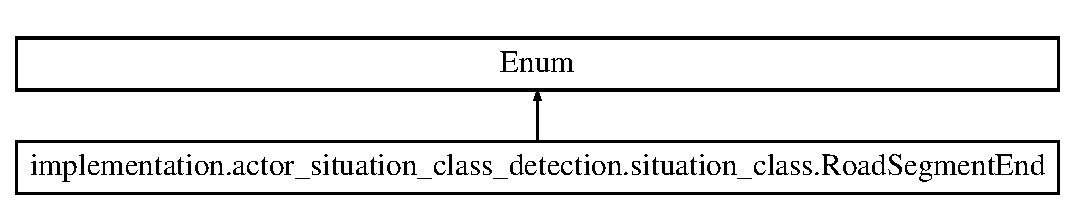
\includegraphics[height=2.000000cm]{classimplementation_1_1actor__situation__class__detection_1_1situation__class_1_1_road_segment_end}
\end{center}
\end{figure}
\subsection*{Static Public Attributes}
\begin{DoxyCompactItemize}
\item 
int \hyperlink{classimplementation_1_1actor__situation__class__detection_1_1situation__class_1_1_road_segment_end_ac236f9ded423a3602b291070ee83c136}{A} = 1
\item 
int \hyperlink{classimplementation_1_1actor__situation__class__detection_1_1situation__class_1_1_road_segment_end_a002ab16ab927773e8aaa6d43868fcd91}{B} = 2
\item 
int \hyperlink{classimplementation_1_1actor__situation__class__detection_1_1situation__class_1_1_road_segment_end_abd9de9ed200ca5cfc4405c83547ca27e}{C} = 3
\item 
int \hyperlink{classimplementation_1_1actor__situation__class__detection_1_1situation__class_1_1_road_segment_end_a87990f0449b67dd6e539d74717f54c58}{D} = 4
\end{DoxyCompactItemize}


\subsection{Member Data Documentation}
\mbox{\Hypertarget{classimplementation_1_1actor__situation__class__detection_1_1situation__class_1_1_road_segment_end_ac236f9ded423a3602b291070ee83c136}\label{classimplementation_1_1actor__situation__class__detection_1_1situation__class_1_1_road_segment_end_ac236f9ded423a3602b291070ee83c136}} 
\index{implementation\+::actor\+\_\+situation\+\_\+class\+\_\+detection\+::situation\+\_\+class\+::\+Road\+Segment\+End@{implementation\+::actor\+\_\+situation\+\_\+class\+\_\+detection\+::situation\+\_\+class\+::\+Road\+Segment\+End}!A@{A}}
\index{A@{A}!implementation\+::actor\+\_\+situation\+\_\+class\+\_\+detection\+::situation\+\_\+class\+::\+Road\+Segment\+End@{implementation\+::actor\+\_\+situation\+\_\+class\+\_\+detection\+::situation\+\_\+class\+::\+Road\+Segment\+End}}
\subsubsection{\texorpdfstring{A}{A}}
{\footnotesize\ttfamily int implementation.\+actor\+\_\+situation\+\_\+class\+\_\+detection.\+situation\+\_\+class.\+Road\+Segment\+End.\+A = 1\hspace{0.3cm}{\ttfamily [static]}}

\mbox{\Hypertarget{classimplementation_1_1actor__situation__class__detection_1_1situation__class_1_1_road_segment_end_a002ab16ab927773e8aaa6d43868fcd91}\label{classimplementation_1_1actor__situation__class__detection_1_1situation__class_1_1_road_segment_end_a002ab16ab927773e8aaa6d43868fcd91}} 
\index{implementation\+::actor\+\_\+situation\+\_\+class\+\_\+detection\+::situation\+\_\+class\+::\+Road\+Segment\+End@{implementation\+::actor\+\_\+situation\+\_\+class\+\_\+detection\+::situation\+\_\+class\+::\+Road\+Segment\+End}!B@{B}}
\index{B@{B}!implementation\+::actor\+\_\+situation\+\_\+class\+\_\+detection\+::situation\+\_\+class\+::\+Road\+Segment\+End@{implementation\+::actor\+\_\+situation\+\_\+class\+\_\+detection\+::situation\+\_\+class\+::\+Road\+Segment\+End}}
\subsubsection{\texorpdfstring{B}{B}}
{\footnotesize\ttfamily int implementation.\+actor\+\_\+situation\+\_\+class\+\_\+detection.\+situation\+\_\+class.\+Road\+Segment\+End.\+B = 2\hspace{0.3cm}{\ttfamily [static]}}

\mbox{\Hypertarget{classimplementation_1_1actor__situation__class__detection_1_1situation__class_1_1_road_segment_end_abd9de9ed200ca5cfc4405c83547ca27e}\label{classimplementation_1_1actor__situation__class__detection_1_1situation__class_1_1_road_segment_end_abd9de9ed200ca5cfc4405c83547ca27e}} 
\index{implementation\+::actor\+\_\+situation\+\_\+class\+\_\+detection\+::situation\+\_\+class\+::\+Road\+Segment\+End@{implementation\+::actor\+\_\+situation\+\_\+class\+\_\+detection\+::situation\+\_\+class\+::\+Road\+Segment\+End}!C@{C}}
\index{C@{C}!implementation\+::actor\+\_\+situation\+\_\+class\+\_\+detection\+::situation\+\_\+class\+::\+Road\+Segment\+End@{implementation\+::actor\+\_\+situation\+\_\+class\+\_\+detection\+::situation\+\_\+class\+::\+Road\+Segment\+End}}
\subsubsection{\texorpdfstring{C}{C}}
{\footnotesize\ttfamily int implementation.\+actor\+\_\+situation\+\_\+class\+\_\+detection.\+situation\+\_\+class.\+Road\+Segment\+End.\+C = 3\hspace{0.3cm}{\ttfamily [static]}}

\mbox{\Hypertarget{classimplementation_1_1actor__situation__class__detection_1_1situation__class_1_1_road_segment_end_a87990f0449b67dd6e539d74717f54c58}\label{classimplementation_1_1actor__situation__class__detection_1_1situation__class_1_1_road_segment_end_a87990f0449b67dd6e539d74717f54c58}} 
\index{implementation\+::actor\+\_\+situation\+\_\+class\+\_\+detection\+::situation\+\_\+class\+::\+Road\+Segment\+End@{implementation\+::actor\+\_\+situation\+\_\+class\+\_\+detection\+::situation\+\_\+class\+::\+Road\+Segment\+End}!D@{D}}
\index{D@{D}!implementation\+::actor\+\_\+situation\+\_\+class\+\_\+detection\+::situation\+\_\+class\+::\+Road\+Segment\+End@{implementation\+::actor\+\_\+situation\+\_\+class\+\_\+detection\+::situation\+\_\+class\+::\+Road\+Segment\+End}}
\subsubsection{\texorpdfstring{D}{D}}
{\footnotesize\ttfamily int implementation.\+actor\+\_\+situation\+\_\+class\+\_\+detection.\+situation\+\_\+class.\+Road\+Segment\+End.\+D = 4\hspace{0.3cm}{\ttfamily [static]}}



The documentation for this class was generated from the following file\+:\begin{DoxyCompactItemize}
\item 
implementation/actor\+\_\+situation\+\_\+class\+\_\+detection/\hyperlink{situation__class_8py}{situation\+\_\+class.\+py}\end{DoxyCompactItemize}

\hypertarget{classimplementation_1_1data__model_1_1positions_1_1_route_position}{}\section{implementation.\+data\+\_\+model.\+positions.\+Route\+Position Class Reference}
\label{classimplementation_1_1data__model_1_1positions_1_1_route_position}\index{implementation.\+data\+\_\+model.\+positions.\+Route\+Position@{implementation.\+data\+\_\+model.\+positions.\+Route\+Position}}
\subsection*{Static Public Attributes}
\begin{DoxyCompactItemize}
\item 
\hyperlink{classimplementation_1_1data__model_1_1positions_1_1_route_position_ac021d8b93dfea605c9dbbe00b1b15599}{Orientation}
\end{DoxyCompactItemize}


\subsection{Member Data Documentation}
\mbox{\Hypertarget{classimplementation_1_1data__model_1_1positions_1_1_route_position_ac021d8b93dfea605c9dbbe00b1b15599}\label{classimplementation_1_1data__model_1_1positions_1_1_route_position_ac021d8b93dfea605c9dbbe00b1b15599}} 
\index{implementation\+::data\+\_\+model\+::positions\+::\+Route\+Position@{implementation\+::data\+\_\+model\+::positions\+::\+Route\+Position}!Orientation@{Orientation}}
\index{Orientation@{Orientation}!implementation\+::data\+\_\+model\+::positions\+::\+Route\+Position@{implementation\+::data\+\_\+model\+::positions\+::\+Route\+Position}}
\subsubsection{\texorpdfstring{Orientation}{Orientation}}
{\footnotesize\ttfamily implementation.\+data\+\_\+model.\+positions.\+Route\+Position.\+Orientation\hspace{0.3cm}{\ttfamily [static]}}



The documentation for this class was generated from the following file\+:\begin{DoxyCompactItemize}
\item 
implementation/data\+\_\+model/\hyperlink{positions_8py}{positions.\+py}\end{DoxyCompactItemize}

\hypertarget{classimplementation_1_1scenarios_1_1carla__scenarios_1_1simple__vehicle__control__adapted_1_1_simple_vehicle_control_adapted}{}\section{implementation.\+scenarios.\+carla\+\_\+scenarios.\+simple\+\_\+vehicle\+\_\+control\+\_\+adapted.\+Simple\+Vehicle\+Control\+Adapted Class Reference}
\label{classimplementation_1_1scenarios_1_1carla__scenarios_1_1simple__vehicle__control__adapted_1_1_simple_vehicle_control_adapted}\index{implementation.\+scenarios.\+carla\+\_\+scenarios.\+simple\+\_\+vehicle\+\_\+control\+\_\+adapted.\+Simple\+Vehicle\+Control\+Adapted@{implementation.\+scenarios.\+carla\+\_\+scenarios.\+simple\+\_\+vehicle\+\_\+control\+\_\+adapted.\+Simple\+Vehicle\+Control\+Adapted}}
Inheritance diagram for implementation.\+scenarios.\+carla\+\_\+scenarios.\+simple\+\_\+vehicle\+\_\+control\+\_\+adapted.\+Simple\+Vehicle\+Control\+Adapted\+:\begin{figure}[H]
\begin{center}
\leavevmode
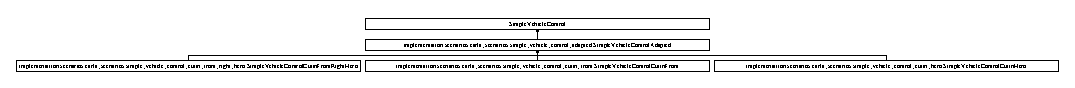
\includegraphics[height=0.737813cm]{classimplementation_1_1scenarios_1_1carla__scenarios_1_1simple__vehicle__control__adapted_1_1_simple_vehicle_control_adapted}
\end{center}
\end{figure}
\subsection*{Public Member Functions}
\begin{DoxyCompactItemize}
\item 
def \hyperlink{classimplementation_1_1scenarios_1_1carla__scenarios_1_1simple__vehicle__control__adapted_1_1_simple_vehicle_control_adapted_ab8480f0c42238a13f8504d84f893b762}{\+\_\+\+\_\+init\+\_\+\+\_\+} (self, actor, args=None)
\item 
def \hyperlink{classimplementation_1_1scenarios_1_1carla__scenarios_1_1simple__vehicle__control__adapted_1_1_simple_vehicle_control_adapted_acc7f8329b0043a22bd7095e7d58ead1b}{run\+\_\+step} (self)
\end{DoxyCompactItemize}


\subsection{Detailed Description}
\begin{DoxyVerb}Controller class for vehicles derived from BasicControl.

The controller directly sets velocities in CARLA, therefore bypassing
CARLA's vehicle engine. This allows a very precise speed control, but comes
with limitations during cornering.

In addition, the controller can consider blocking obstacles, which are
classified as dynamic (i.e. vehicles, bikes, pedestrians). Activation of this
features is controlled by passing proper arguments to the class constructor.
The collision detection uses CARLA's obstacle sensor (sensor.other.obstacle),
which checks for obstacles in the direct forward channel of the vehicle, i.e.
there are limitation with sideways obstacles and while cornering.

Args:
    actor (carla.Actor): Vehicle actor that should be controlled.
    args (dictionary): Dictonary of (key, value) arguments to be used by the controller.
                       May include: (consider_obstacles, true/false) - Enable consideration of obstacles
                                    (proximity_threshold, distance)  - Distance in front of actor in which
                                                                       obstacles are considered
                                    (attach_camera, true/false)      - Attach OpenCV display to actor
                                                                       (useful for debugging)

Attributes:

    _generated_waypoint_list (list of carla.Transform): List of target waypoints the actor
        should travel along. A waypoint here is of type carla.Transform!
        Defaults to [].
    _last_update (float): Last time step the update function (tick()) was called.
        Defaults to None.
    _consider_obstacles (boolean): Enable/Disable consideration of obstacles
        Defaults to False.
    _proximity_threshold (float): Distance in front of actor in which obstacles are considered
        Defaults to infinity.
    _cv_image (CV Image): Contains the OpenCV image, in case a debug camera is attached to the actor
        Defaults to None.
    _camera (sensor.camera.rgb): Debug camera attached to actor
        Defaults to None.
    _obstacle_sensor (sensor.other.obstacle): Obstacle sensor attached to actor
        Defaults to None.
    _obstacle_distance (float): Distance of the closest obstacle returned by the obstacle sensor
        Defaults to infinity.
    _obstacle_actor (carla.Actor): Closest obstacle returned by the obstacle sensor
        Defaults to None.
\end{DoxyVerb}
 

\subsection{Constructor \& Destructor Documentation}
\mbox{\Hypertarget{classimplementation_1_1scenarios_1_1carla__scenarios_1_1simple__vehicle__control__adapted_1_1_simple_vehicle_control_adapted_ab8480f0c42238a13f8504d84f893b762}\label{classimplementation_1_1scenarios_1_1carla__scenarios_1_1simple__vehicle__control__adapted_1_1_simple_vehicle_control_adapted_ab8480f0c42238a13f8504d84f893b762}} 
\index{implementation\+::scenarios\+::carla\+\_\+scenarios\+::simple\+\_\+vehicle\+\_\+control\+\_\+adapted\+::\+Simple\+Vehicle\+Control\+Adapted@{implementation\+::scenarios\+::carla\+\_\+scenarios\+::simple\+\_\+vehicle\+\_\+control\+\_\+adapted\+::\+Simple\+Vehicle\+Control\+Adapted}!\+\_\+\+\_\+init\+\_\+\+\_\+@{\+\_\+\+\_\+init\+\_\+\+\_\+}}
\index{\+\_\+\+\_\+init\+\_\+\+\_\+@{\+\_\+\+\_\+init\+\_\+\+\_\+}!implementation\+::scenarios\+::carla\+\_\+scenarios\+::simple\+\_\+vehicle\+\_\+control\+\_\+adapted\+::\+Simple\+Vehicle\+Control\+Adapted@{implementation\+::scenarios\+::carla\+\_\+scenarios\+::simple\+\_\+vehicle\+\_\+control\+\_\+adapted\+::\+Simple\+Vehicle\+Control\+Adapted}}
\subsubsection{\texorpdfstring{\+\_\+\+\_\+init\+\_\+\+\_\+()}{\_\_init\_\_()}}
{\footnotesize\ttfamily def implementation.\+scenarios.\+carla\+\_\+scenarios.\+simple\+\_\+vehicle\+\_\+control\+\_\+adapted.\+Simple\+Vehicle\+Control\+Adapted.\+\_\+\+\_\+init\+\_\+\+\_\+ (\begin{DoxyParamCaption}\item[{}]{self,  }\item[{}]{actor,  }\item[{}]{args = {\ttfamily None} }\end{DoxyParamCaption})}



\subsection{Member Function Documentation}
\mbox{\Hypertarget{classimplementation_1_1scenarios_1_1carla__scenarios_1_1simple__vehicle__control__adapted_1_1_simple_vehicle_control_adapted_acc7f8329b0043a22bd7095e7d58ead1b}\label{classimplementation_1_1scenarios_1_1carla__scenarios_1_1simple__vehicle__control__adapted_1_1_simple_vehicle_control_adapted_acc7f8329b0043a22bd7095e7d58ead1b}} 
\index{implementation\+::scenarios\+::carla\+\_\+scenarios\+::simple\+\_\+vehicle\+\_\+control\+\_\+adapted\+::\+Simple\+Vehicle\+Control\+Adapted@{implementation\+::scenarios\+::carla\+\_\+scenarios\+::simple\+\_\+vehicle\+\_\+control\+\_\+adapted\+::\+Simple\+Vehicle\+Control\+Adapted}!run\+\_\+step@{run\+\_\+step}}
\index{run\+\_\+step@{run\+\_\+step}!implementation\+::scenarios\+::carla\+\_\+scenarios\+::simple\+\_\+vehicle\+\_\+control\+\_\+adapted\+::\+Simple\+Vehicle\+Control\+Adapted@{implementation\+::scenarios\+::carla\+\_\+scenarios\+::simple\+\_\+vehicle\+\_\+control\+\_\+adapted\+::\+Simple\+Vehicle\+Control\+Adapted}}
\subsubsection{\texorpdfstring{run\+\_\+step()}{run\_step()}}
{\footnotesize\ttfamily def implementation.\+scenarios.\+carla\+\_\+scenarios.\+simple\+\_\+vehicle\+\_\+control\+\_\+adapted.\+Simple\+Vehicle\+Control\+Adapted.\+run\+\_\+step (\begin{DoxyParamCaption}\item[{}]{self }\end{DoxyParamCaption})}

\begin{DoxyVerb}Execute on tick of the controller's control loop

If _waypoints are provided, the vehicle moves towards the next waypoint
with the given _target_speed, until reaching the final waypoint. Upon reaching
the final waypoint, _reached_goal is set to True.

If _waypoints is empty, the vehicle moves in its current direction with
the given _target_speed.

For further details see :func:`_set_new_velocity`
\end{DoxyVerb}
 

The documentation for this class was generated from the following file\+:\begin{DoxyCompactItemize}
\item 
implementation/scenarios/carla\+\_\+scenarios/\hyperlink{simple__vehicle__control__adapted_8py}{simple\+\_\+vehicle\+\_\+control\+\_\+adapted.\+py}\end{DoxyCompactItemize}

\hypertarget{classimplementation_1_1scenarios_1_1carla__scenarios_1_1simple__vehicle__control__cutin__from__r6474a3ad40f8613a989008f8fef990bd}{}\section{implementation.\+scenarios.\+carla\+\_\+scenarios.\+simple\+\_\+vehicle\+\_\+control\+\_\+cutin\+\_\+from\+\_\+right\+\_\+hero.\+Simple\+Vehicle\+Control\+Cutin\+From\+Right\+Hero Class Reference}
\label{classimplementation_1_1scenarios_1_1carla__scenarios_1_1simple__vehicle__control__cutin__from__r6474a3ad40f8613a989008f8fef990bd}\index{implementation.\+scenarios.\+carla\+\_\+scenarios.\+simple\+\_\+vehicle\+\_\+control\+\_\+cutin\+\_\+from\+\_\+right\+\_\+hero.\+Simple\+Vehicle\+Control\+Cutin\+From\+Right\+Hero@{implementation.\+scenarios.\+carla\+\_\+scenarios.\+simple\+\_\+vehicle\+\_\+control\+\_\+cutin\+\_\+from\+\_\+right\+\_\+hero.\+Simple\+Vehicle\+Control\+Cutin\+From\+Right\+Hero}}
Inheritance diagram for implementation.\+scenarios.\+carla\+\_\+scenarios.\+simple\+\_\+vehicle\+\_\+control\+\_\+cutin\+\_\+from\+\_\+right\+\_\+hero.\+Simple\+Vehicle\+Control\+Cutin\+From\+Right\+Hero\+:\begin{figure}[H]
\begin{center}
\leavevmode
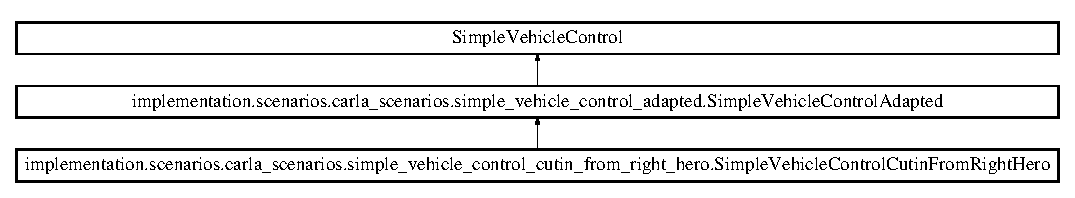
\includegraphics[height=2.213439cm]{classimplementation_1_1scenarios_1_1carla__scenarios_1_1simple__vehicle__control__cutin__from__r6474a3ad40f8613a989008f8fef990bd}
\end{center}
\end{figure}
\subsection*{Public Member Functions}
\begin{DoxyCompactItemize}
\item 
def \hyperlink{classimplementation_1_1scenarios_1_1carla__scenarios_1_1simple__vehicle__control__cutin__from__r6474a3ad40f8613a989008f8fef990bd_a43f2d387cd473b56e2e2739b10ee8b27}{run\+\_\+step} (self)
\end{DoxyCompactItemize}


\subsection{Member Function Documentation}
\mbox{\Hypertarget{classimplementation_1_1scenarios_1_1carla__scenarios_1_1simple__vehicle__control__cutin__from__r6474a3ad40f8613a989008f8fef990bd_a43f2d387cd473b56e2e2739b10ee8b27}\label{classimplementation_1_1scenarios_1_1carla__scenarios_1_1simple__vehicle__control__cutin__from__r6474a3ad40f8613a989008f8fef990bd_a43f2d387cd473b56e2e2739b10ee8b27}} 
\index{implementation\+::scenarios\+::carla\+\_\+scenarios\+::simple\+\_\+vehicle\+\_\+control\+\_\+cutin\+\_\+from\+\_\+right\+\_\+hero\+::\+Simple\+Vehicle\+Control\+Cutin\+From\+Right\+Hero@{implementation\+::scenarios\+::carla\+\_\+scenarios\+::simple\+\_\+vehicle\+\_\+control\+\_\+cutin\+\_\+from\+\_\+right\+\_\+hero\+::\+Simple\+Vehicle\+Control\+Cutin\+From\+Right\+Hero}!run\+\_\+step@{run\+\_\+step}}
\index{run\+\_\+step@{run\+\_\+step}!implementation\+::scenarios\+::carla\+\_\+scenarios\+::simple\+\_\+vehicle\+\_\+control\+\_\+cutin\+\_\+from\+\_\+right\+\_\+hero\+::\+Simple\+Vehicle\+Control\+Cutin\+From\+Right\+Hero@{implementation\+::scenarios\+::carla\+\_\+scenarios\+::simple\+\_\+vehicle\+\_\+control\+\_\+cutin\+\_\+from\+\_\+right\+\_\+hero\+::\+Simple\+Vehicle\+Control\+Cutin\+From\+Right\+Hero}}
\subsubsection{\texorpdfstring{run\+\_\+step()}{run\_step()}}
{\footnotesize\ttfamily def implementation.\+scenarios.\+carla\+\_\+scenarios.\+simple\+\_\+vehicle\+\_\+control\+\_\+cutin\+\_\+from\+\_\+right\+\_\+hero.\+Simple\+Vehicle\+Control\+Cutin\+From\+Right\+Hero.\+run\+\_\+step (\begin{DoxyParamCaption}\item[{}]{self }\end{DoxyParamCaption})}



The documentation for this class was generated from the following file\+:\begin{DoxyCompactItemize}
\item 
implementation/scenarios/carla\+\_\+scenarios/\hyperlink{simple__vehicle__control__cutin__from__right__hero_8py}{simple\+\_\+vehicle\+\_\+control\+\_\+cutin\+\_\+from\+\_\+right\+\_\+hero.\+py}\end{DoxyCompactItemize}

\hypertarget{classimplementation_1_1scenarios_1_1carla__scenarios_1_1simple__vehicle__control__cutin__front_14eb2b3a85937f52b63b15ef53e9a1f6e}{}\section{implementation.\+scenarios.\+carla\+\_\+scenarios.\+simple\+\_\+vehicle\+\_\+control\+\_\+cutin\+\_\+front.\+Simple\+Vehicle\+Control\+Cutin\+Front Class Reference}
\label{classimplementation_1_1scenarios_1_1carla__scenarios_1_1simple__vehicle__control__cutin__front_14eb2b3a85937f52b63b15ef53e9a1f6e}\index{implementation.\+scenarios.\+carla\+\_\+scenarios.\+simple\+\_\+vehicle\+\_\+control\+\_\+cutin\+\_\+front.\+Simple\+Vehicle\+Control\+Cutin\+Front@{implementation.\+scenarios.\+carla\+\_\+scenarios.\+simple\+\_\+vehicle\+\_\+control\+\_\+cutin\+\_\+front.\+Simple\+Vehicle\+Control\+Cutin\+Front}}
Inheritance diagram for implementation.\+scenarios.\+carla\+\_\+scenarios.\+simple\+\_\+vehicle\+\_\+control\+\_\+cutin\+\_\+front.\+Simple\+Vehicle\+Control\+Cutin\+Front\+:\begin{figure}[H]
\begin{center}
\leavevmode
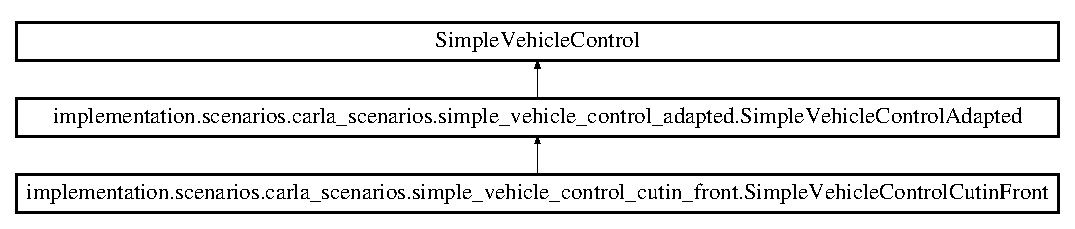
\includegraphics[height=2.625000cm]{classimplementation_1_1scenarios_1_1carla__scenarios_1_1simple__vehicle__control__cutin__front_14eb2b3a85937f52b63b15ef53e9a1f6e}
\end{center}
\end{figure}
\subsection*{Public Member Functions}
\begin{DoxyCompactItemize}
\item 
def \hyperlink{classimplementation_1_1scenarios_1_1carla__scenarios_1_1simple__vehicle__control__cutin__front_14eb2b3a85937f52b63b15ef53e9a1f6e_ac87a8a7af06b9d3990992088a9a56e51}{run\+\_\+step} (self)
\end{DoxyCompactItemize}


\subsection{Member Function Documentation}
\mbox{\Hypertarget{classimplementation_1_1scenarios_1_1carla__scenarios_1_1simple__vehicle__control__cutin__front_14eb2b3a85937f52b63b15ef53e9a1f6e_ac87a8a7af06b9d3990992088a9a56e51}\label{classimplementation_1_1scenarios_1_1carla__scenarios_1_1simple__vehicle__control__cutin__front_14eb2b3a85937f52b63b15ef53e9a1f6e_ac87a8a7af06b9d3990992088a9a56e51}} 
\index{implementation\+::scenarios\+::carla\+\_\+scenarios\+::simple\+\_\+vehicle\+\_\+control\+\_\+cutin\+\_\+front\+::\+Simple\+Vehicle\+Control\+Cutin\+Front@{implementation\+::scenarios\+::carla\+\_\+scenarios\+::simple\+\_\+vehicle\+\_\+control\+\_\+cutin\+\_\+front\+::\+Simple\+Vehicle\+Control\+Cutin\+Front}!run\+\_\+step@{run\+\_\+step}}
\index{run\+\_\+step@{run\+\_\+step}!implementation\+::scenarios\+::carla\+\_\+scenarios\+::simple\+\_\+vehicle\+\_\+control\+\_\+cutin\+\_\+front\+::\+Simple\+Vehicle\+Control\+Cutin\+Front@{implementation\+::scenarios\+::carla\+\_\+scenarios\+::simple\+\_\+vehicle\+\_\+control\+\_\+cutin\+\_\+front\+::\+Simple\+Vehicle\+Control\+Cutin\+Front}}
\subsubsection{\texorpdfstring{run\+\_\+step()}{run\_step()}}
{\footnotesize\ttfamily def implementation.\+scenarios.\+carla\+\_\+scenarios.\+simple\+\_\+vehicle\+\_\+control\+\_\+cutin\+\_\+front.\+Simple\+Vehicle\+Control\+Cutin\+Front.\+run\+\_\+step (\begin{DoxyParamCaption}\item[{}]{self }\end{DoxyParamCaption})}



The documentation for this class was generated from the following file\+:\begin{DoxyCompactItemize}
\item 
implementation/scenarios/carla\+\_\+scenarios/\hyperlink{simple__vehicle__control__cutin__front_8py}{simple\+\_\+vehicle\+\_\+control\+\_\+cutin\+\_\+front.\+py}\end{DoxyCompactItemize}

\hypertarget{classimplementation_1_1scenarios_1_1carla__scenarios_1_1simple__vehicle__control__cutin__hero_1_11e90bc75d1539d6c07dc5179559d6d0}{}\section{implementation.\+scenarios.\+carla\+\_\+scenarios.\+simple\+\_\+vehicle\+\_\+control\+\_\+cutin\+\_\+hero.\+Simple\+Vehicle\+Control\+Cutin\+Hero Class Reference}
\label{classimplementation_1_1scenarios_1_1carla__scenarios_1_1simple__vehicle__control__cutin__hero_1_11e90bc75d1539d6c07dc5179559d6d0}\index{implementation.\+scenarios.\+carla\+\_\+scenarios.\+simple\+\_\+vehicle\+\_\+control\+\_\+cutin\+\_\+hero.\+Simple\+Vehicle\+Control\+Cutin\+Hero@{implementation.\+scenarios.\+carla\+\_\+scenarios.\+simple\+\_\+vehicle\+\_\+control\+\_\+cutin\+\_\+hero.\+Simple\+Vehicle\+Control\+Cutin\+Hero}}
Inheritance diagram for implementation.\+scenarios.\+carla\+\_\+scenarios.\+simple\+\_\+vehicle\+\_\+control\+\_\+cutin\+\_\+hero.\+Simple\+Vehicle\+Control\+Cutin\+Hero\+:\begin{figure}[H]
\begin{center}
\leavevmode
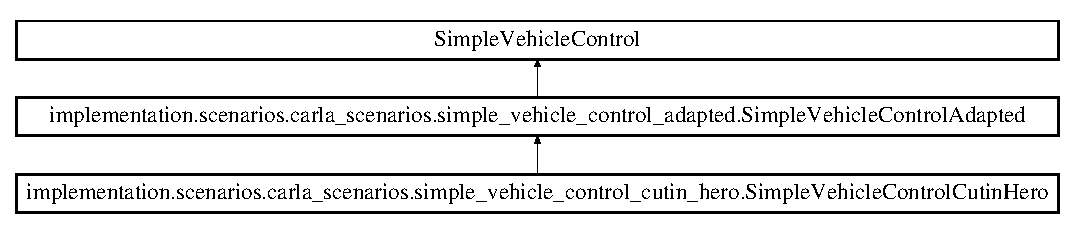
\includegraphics[height=2.633229cm]{classimplementation_1_1scenarios_1_1carla__scenarios_1_1simple__vehicle__control__cutin__hero_1_11e90bc75d1539d6c07dc5179559d6d0}
\end{center}
\end{figure}
\subsection*{Public Member Functions}
\begin{DoxyCompactItemize}
\item 
def \hyperlink{classimplementation_1_1scenarios_1_1carla__scenarios_1_1simple__vehicle__control__cutin__hero_1_11e90bc75d1539d6c07dc5179559d6d0_a770942881c3cd7ebb8a54e5b82eb4b5d}{run\+\_\+step} (self)
\end{DoxyCompactItemize}


\subsection{Member Function Documentation}
\mbox{\Hypertarget{classimplementation_1_1scenarios_1_1carla__scenarios_1_1simple__vehicle__control__cutin__hero_1_11e90bc75d1539d6c07dc5179559d6d0_a770942881c3cd7ebb8a54e5b82eb4b5d}\label{classimplementation_1_1scenarios_1_1carla__scenarios_1_1simple__vehicle__control__cutin__hero_1_11e90bc75d1539d6c07dc5179559d6d0_a770942881c3cd7ebb8a54e5b82eb4b5d}} 
\index{implementation\+::scenarios\+::carla\+\_\+scenarios\+::simple\+\_\+vehicle\+\_\+control\+\_\+cutin\+\_\+hero\+::\+Simple\+Vehicle\+Control\+Cutin\+Hero@{implementation\+::scenarios\+::carla\+\_\+scenarios\+::simple\+\_\+vehicle\+\_\+control\+\_\+cutin\+\_\+hero\+::\+Simple\+Vehicle\+Control\+Cutin\+Hero}!run\+\_\+step@{run\+\_\+step}}
\index{run\+\_\+step@{run\+\_\+step}!implementation\+::scenarios\+::carla\+\_\+scenarios\+::simple\+\_\+vehicle\+\_\+control\+\_\+cutin\+\_\+hero\+::\+Simple\+Vehicle\+Control\+Cutin\+Hero@{implementation\+::scenarios\+::carla\+\_\+scenarios\+::simple\+\_\+vehicle\+\_\+control\+\_\+cutin\+\_\+hero\+::\+Simple\+Vehicle\+Control\+Cutin\+Hero}}
\subsubsection{\texorpdfstring{run\+\_\+step()}{run\_step()}}
{\footnotesize\ttfamily def implementation.\+scenarios.\+carla\+\_\+scenarios.\+simple\+\_\+vehicle\+\_\+control\+\_\+cutin\+\_\+hero.\+Simple\+Vehicle\+Control\+Cutin\+Hero.\+run\+\_\+step (\begin{DoxyParamCaption}\item[{}]{self }\end{DoxyParamCaption})}



The documentation for this class was generated from the following file\+:\begin{DoxyCompactItemize}
\item 
implementation/scenarios/carla\+\_\+scenarios/\hyperlink{simple__vehicle__control__cutin__hero_8py}{simple\+\_\+vehicle\+\_\+control\+\_\+cutin\+\_\+hero.\+py}\end{DoxyCompactItemize}

\hypertarget{classimplementation_1_1simulators_1_1simulator__controller_1_1_simulator_controller}{}\section{implementation.\+simulators.\+simulator\+\_\+controller.\+Simulator\+Controller Class Reference}
\label{classimplementation_1_1simulators_1_1simulator__controller_1_1_simulator_controller}\index{implementation.\+simulators.\+simulator\+\_\+controller.\+Simulator\+Controller@{implementation.\+simulators.\+simulator\+\_\+controller.\+Simulator\+Controller}}
Inheritance diagram for implementation.\+simulators.\+simulator\+\_\+controller.\+Simulator\+Controller\+:\begin{figure}[H]
\begin{center}
\leavevmode
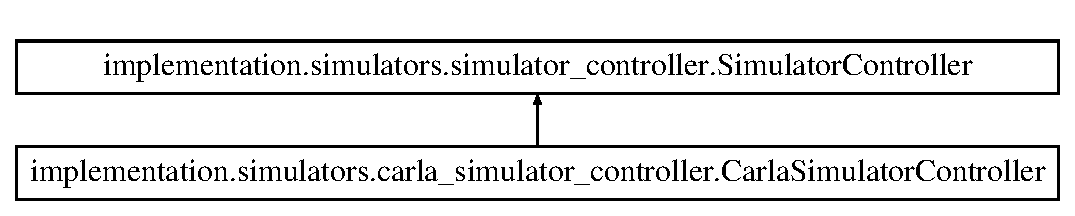
\includegraphics[height=2.000000cm]{classimplementation_1_1simulators_1_1simulator__controller_1_1_simulator_controller}
\end{center}
\end{figure}
\subsection*{Public Member Functions}
\begin{DoxyCompactItemize}
\item 
def \hyperlink{classimplementation_1_1simulators_1_1simulator__controller_1_1_simulator_controller_a7712a41b0eb99c1708c3d3b8fa857333}{connect\+\_\+simulator} (self)
\item 
def \hyperlink{classimplementation_1_1simulators_1_1simulator__controller_1_1_simulator_controller_a7c2a65ff6436876710a4ca3c9c976d27}{setup\+\_\+simulator} (self)
\item 
def \hyperlink{classimplementation_1_1simulators_1_1simulator__controller_1_1_simulator_controller_a8e44240be7fae6640ce790bf2e765564}{run\+\_\+simulator\+\_\+game\+\_\+loop\+\_\+step} (self)
\item 
def \hyperlink{classimplementation_1_1simulators_1_1simulator__controller_1_1_simulator_controller_a9f7953e17973cf3895b85dd132f56d5a}{get\+\_\+sinadra\+\_\+data} (self)
\item 
def \hyperlink{classimplementation_1_1simulators_1_1simulator__controller_1_1_simulator_controller_ad24f6ec1fe6ec1b13da2b3183f98dcb6}{get\+\_\+map} (self)
\item 
def \hyperlink{classimplementation_1_1simulators_1_1simulator__controller_1_1_simulator_controller_a60cbb121b4c001e8cf0073676170d45c}{get\+\_\+scenario\+\_\+image} (self)
\item 
def \hyperlink{classimplementation_1_1simulators_1_1simulator__controller_1_1_simulator_controller_a3f8215746649fb87dae9308e663ebd88}{get\+\_\+subject\+\_\+vehicle\+\_\+image} (self)
\item 
def \hyperlink{classimplementation_1_1simulators_1_1simulator__controller_1_1_simulator_controller_a2145a4a7f793f3a172c567b2b0d626c1}{draw\+\_\+line}
\end{DoxyCompactItemize}


\subsection{Member Function Documentation}
\mbox{\Hypertarget{classimplementation_1_1simulators_1_1simulator__controller_1_1_simulator_controller_a7712a41b0eb99c1708c3d3b8fa857333}\label{classimplementation_1_1simulators_1_1simulator__controller_1_1_simulator_controller_a7712a41b0eb99c1708c3d3b8fa857333}} 
\index{implementation\+::simulators\+::simulator\+\_\+controller\+::\+Simulator\+Controller@{implementation\+::simulators\+::simulator\+\_\+controller\+::\+Simulator\+Controller}!connect\+\_\+simulator@{connect\+\_\+simulator}}
\index{connect\+\_\+simulator@{connect\+\_\+simulator}!implementation\+::simulators\+::simulator\+\_\+controller\+::\+Simulator\+Controller@{implementation\+::simulators\+::simulator\+\_\+controller\+::\+Simulator\+Controller}}
\subsubsection{\texorpdfstring{connect\+\_\+simulator()}{connect\_simulator()}}
{\footnotesize\ttfamily def implementation.\+simulators.\+simulator\+\_\+controller.\+Simulator\+Controller.\+connect\+\_\+simulator (\begin{DoxyParamCaption}\item[{}]{self,  }\item[{}]{None }\end{DoxyParamCaption})}

\begin{DoxyVerb}Connects the simulator client to the running simulator server instance.\end{DoxyVerb}
 \mbox{\Hypertarget{classimplementation_1_1simulators_1_1simulator__controller_1_1_simulator_controller_a2145a4a7f793f3a172c567b2b0d626c1}\label{classimplementation_1_1simulators_1_1simulator__controller_1_1_simulator_controller_a2145a4a7f793f3a172c567b2b0d626c1}} 
\index{implementation\+::simulators\+::simulator\+\_\+controller\+::\+Simulator\+Controller@{implementation\+::simulators\+::simulator\+\_\+controller\+::\+Simulator\+Controller}!draw\+\_\+line@{draw\+\_\+line}}
\index{draw\+\_\+line@{draw\+\_\+line}!implementation\+::simulators\+::simulator\+\_\+controller\+::\+Simulator\+Controller@{implementation\+::simulators\+::simulator\+\_\+controller\+::\+Simulator\+Controller}}
\subsubsection{\texorpdfstring{draw\+\_\+line()}{draw\_line()}}
{\footnotesize\ttfamily def implementation.\+simulators.\+simulator\+\_\+controller.\+Simulator\+Controller.\+draw\+\_\+line (\begin{DoxyParamCaption}\item[{}]{self,  }\item[{}]{start }\end{DoxyParamCaption})}

\mbox{\Hypertarget{classimplementation_1_1simulators_1_1simulator__controller_1_1_simulator_controller_ad24f6ec1fe6ec1b13da2b3183f98dcb6}\label{classimplementation_1_1simulators_1_1simulator__controller_1_1_simulator_controller_ad24f6ec1fe6ec1b13da2b3183f98dcb6}} 
\index{implementation\+::simulators\+::simulator\+\_\+controller\+::\+Simulator\+Controller@{implementation\+::simulators\+::simulator\+\_\+controller\+::\+Simulator\+Controller}!get\+\_\+map@{get\+\_\+map}}
\index{get\+\_\+map@{get\+\_\+map}!implementation\+::simulators\+::simulator\+\_\+controller\+::\+Simulator\+Controller@{implementation\+::simulators\+::simulator\+\_\+controller\+::\+Simulator\+Controller}}
\subsubsection{\texorpdfstring{get\+\_\+map()}{get\_map()}}
{\footnotesize\ttfamily def implementation.\+simulators.\+simulator\+\_\+controller.\+Simulator\+Controller.\+get\+\_\+map (\begin{DoxyParamCaption}\item[{}]{self,  }\item[{}]{Map }\end{DoxyParamCaption})}

\begin{DoxyVerb}Extracts and Returns the map of the simulator. Typically, done once in the initialization due to the map
being invariant and slow to load.

Returns
-------
Map
    Map SINADRA data object of the simulator.
\end{DoxyVerb}
 \mbox{\Hypertarget{classimplementation_1_1simulators_1_1simulator__controller_1_1_simulator_controller_a60cbb121b4c001e8cf0073676170d45c}\label{classimplementation_1_1simulators_1_1simulator__controller_1_1_simulator_controller_a60cbb121b4c001e8cf0073676170d45c}} 
\index{implementation\+::simulators\+::simulator\+\_\+controller\+::\+Simulator\+Controller@{implementation\+::simulators\+::simulator\+\_\+controller\+::\+Simulator\+Controller}!get\+\_\+scenario\+\_\+image@{get\+\_\+scenario\+\_\+image}}
\index{get\+\_\+scenario\+\_\+image@{get\+\_\+scenario\+\_\+image}!implementation\+::simulators\+::simulator\+\_\+controller\+::\+Simulator\+Controller@{implementation\+::simulators\+::simulator\+\_\+controller\+::\+Simulator\+Controller}}
\subsubsection{\texorpdfstring{get\+\_\+scenario\+\_\+image()}{get\_scenario\_image()}}
{\footnotesize\ttfamily def implementation.\+simulators.\+simulator\+\_\+controller.\+Simulator\+Controller.\+get\+\_\+scenario\+\_\+image (\begin{DoxyParamCaption}\item[{}]{self,  }\item[{}]{Optional,  }\item[{}]{np,  }\item[{}]{ndarray }\end{DoxyParamCaption})}

\begin{DoxyVerb}Extracts and Returns a top view image of the area of interest.

Returns
-------
Optional[np.ndarray]
    Image as a numpy ndarray if the vehicles are already instantiated. If the vehicles are not instantiated yet,
    e.g., if a scenario is not launched already, None is returned instead.
\end{DoxyVerb}
 \mbox{\Hypertarget{classimplementation_1_1simulators_1_1simulator__controller_1_1_simulator_controller_a9f7953e17973cf3895b85dd132f56d5a}\label{classimplementation_1_1simulators_1_1simulator__controller_1_1_simulator_controller_a9f7953e17973cf3895b85dd132f56d5a}} 
\index{implementation\+::simulators\+::simulator\+\_\+controller\+::\+Simulator\+Controller@{implementation\+::simulators\+::simulator\+\_\+controller\+::\+Simulator\+Controller}!get\+\_\+sinadra\+\_\+data@{get\+\_\+sinadra\+\_\+data}}
\index{get\+\_\+sinadra\+\_\+data@{get\+\_\+sinadra\+\_\+data}!implementation\+::simulators\+::simulator\+\_\+controller\+::\+Simulator\+Controller@{implementation\+::simulators\+::simulator\+\_\+controller\+::\+Simulator\+Controller}}
\subsubsection{\texorpdfstring{get\+\_\+sinadra\+\_\+data()}{get\_sinadra\_data()}}
{\footnotesize\ttfamily def implementation.\+simulators.\+simulator\+\_\+controller.\+Simulator\+Controller.\+get\+\_\+sinadra\+\_\+data (\begin{DoxyParamCaption}\item[{}]{self,  }\item[{}]{Optional,  }\item[{}]{Sinadra\+Data }\end{DoxyParamCaption})}

\begin{DoxyVerb}Extracts and Returns the latest SINADRA data (environment and all entities) of the current simulation
step.

Returns
-------
Optional[SinadraData]
    SINADRA data object if the vehicles are already instantiated. If the vehicles are not instantiated yet,
    e.g., if a scenario is not launched already, None is returned instead.
\end{DoxyVerb}
 \mbox{\Hypertarget{classimplementation_1_1simulators_1_1simulator__controller_1_1_simulator_controller_a3f8215746649fb87dae9308e663ebd88}\label{classimplementation_1_1simulators_1_1simulator__controller_1_1_simulator_controller_a3f8215746649fb87dae9308e663ebd88}} 
\index{implementation\+::simulators\+::simulator\+\_\+controller\+::\+Simulator\+Controller@{implementation\+::simulators\+::simulator\+\_\+controller\+::\+Simulator\+Controller}!get\+\_\+subject\+\_\+vehicle\+\_\+image@{get\+\_\+subject\+\_\+vehicle\+\_\+image}}
\index{get\+\_\+subject\+\_\+vehicle\+\_\+image@{get\+\_\+subject\+\_\+vehicle\+\_\+image}!implementation\+::simulators\+::simulator\+\_\+controller\+::\+Simulator\+Controller@{implementation\+::simulators\+::simulator\+\_\+controller\+::\+Simulator\+Controller}}
\subsubsection{\texorpdfstring{get\+\_\+subject\+\_\+vehicle\+\_\+image()}{get\_subject\_vehicle\_image()}}
{\footnotesize\ttfamily def implementation.\+simulators.\+simulator\+\_\+controller.\+Simulator\+Controller.\+get\+\_\+subject\+\_\+vehicle\+\_\+image (\begin{DoxyParamCaption}\item[{}]{self,  }\item[{}]{Optional,  }\item[{}]{np,  }\item[{}]{ndarray }\end{DoxyParamCaption})}

\begin{DoxyVerb}Extracts and Returns an image of the subject vehicle's perspective.

Returns
-------
Optional[np.ndarray]
    Image as a numpy ndarray if the vehicles are already instantiated. If the vehicles are not instantiated yet,
    e.g., if a scenario is not launched already, None is returned instead.
\end{DoxyVerb}
 \mbox{\Hypertarget{classimplementation_1_1simulators_1_1simulator__controller_1_1_simulator_controller_a8e44240be7fae6640ce790bf2e765564}\label{classimplementation_1_1simulators_1_1simulator__controller_1_1_simulator_controller_a8e44240be7fae6640ce790bf2e765564}} 
\index{implementation\+::simulators\+::simulator\+\_\+controller\+::\+Simulator\+Controller@{implementation\+::simulators\+::simulator\+\_\+controller\+::\+Simulator\+Controller}!run\+\_\+simulator\+\_\+game\+\_\+loop\+\_\+step@{run\+\_\+simulator\+\_\+game\+\_\+loop\+\_\+step}}
\index{run\+\_\+simulator\+\_\+game\+\_\+loop\+\_\+step@{run\+\_\+simulator\+\_\+game\+\_\+loop\+\_\+step}!implementation\+::simulators\+::simulator\+\_\+controller\+::\+Simulator\+Controller@{implementation\+::simulators\+::simulator\+\_\+controller\+::\+Simulator\+Controller}}
\subsubsection{\texorpdfstring{run\+\_\+simulator\+\_\+game\+\_\+loop\+\_\+step()}{run\_simulator\_game\_loop\_step()}}
{\footnotesize\ttfamily def implementation.\+simulators.\+simulator\+\_\+controller.\+Simulator\+Controller.\+run\+\_\+simulator\+\_\+game\+\_\+loop\+\_\+step (\begin{DoxyParamCaption}\item[{}]{self,  }\item[{}]{None }\end{DoxyParamCaption})}

\begin{DoxyVerb}Runs one simulation tick of the simulator. Must be called every computation cycle (must align with the
FRAMERATE configuration parameter).
\end{DoxyVerb}
 \mbox{\Hypertarget{classimplementation_1_1simulators_1_1simulator__controller_1_1_simulator_controller_a7c2a65ff6436876710a4ca3c9c976d27}\label{classimplementation_1_1simulators_1_1simulator__controller_1_1_simulator_controller_a7c2a65ff6436876710a4ca3c9c976d27}} 
\index{implementation\+::simulators\+::simulator\+\_\+controller\+::\+Simulator\+Controller@{implementation\+::simulators\+::simulator\+\_\+controller\+::\+Simulator\+Controller}!setup\+\_\+simulator@{setup\+\_\+simulator}}
\index{setup\+\_\+simulator@{setup\+\_\+simulator}!implementation\+::simulators\+::simulator\+\_\+controller\+::\+Simulator\+Controller@{implementation\+::simulators\+::simulator\+\_\+controller\+::\+Simulator\+Controller}}
\subsubsection{\texorpdfstring{setup\+\_\+simulator()}{setup\_simulator()}}
{\footnotesize\ttfamily def implementation.\+simulators.\+simulator\+\_\+controller.\+Simulator\+Controller.\+setup\+\_\+simulator (\begin{DoxyParamCaption}\item[{}]{self,  }\item[{}]{None }\end{DoxyParamCaption})}

\begin{DoxyVerb}Sets up the simulator client for running evaluation scenarios.\end{DoxyVerb}
 

The documentation for this class was generated from the following file\+:\begin{DoxyCompactItemize}
\item 
implementation/simulators/\hyperlink{simulator__controller_8py}{simulator\+\_\+controller.\+py}\end{DoxyCompactItemize}

\hypertarget{classimplementation_1_1sinadra__risk__sensor__client_1_1_sinadra_client}{}\section{implementation.\+sinadra\+\_\+risk\+\_\+sensor\+\_\+client.\+Sinadra\+Client Class Reference}
\label{classimplementation_1_1sinadra__risk__sensor__client_1_1_sinadra_client}\index{implementation.\+sinadra\+\_\+risk\+\_\+sensor\+\_\+client.\+Sinadra\+Client@{implementation.\+sinadra\+\_\+risk\+\_\+sensor\+\_\+client.\+Sinadra\+Client}}
\subsection*{Public Member Functions}
\begin{DoxyCompactItemize}
\item 
def \hyperlink{classimplementation_1_1sinadra__risk__sensor__client_1_1_sinadra_client_a84329d20e8b5e7455783f51edd03bcf5}{\+\_\+\+\_\+init\+\_\+\+\_\+}
\item 
def \hyperlink{classimplementation_1_1sinadra__risk__sensor__client_1_1_sinadra_client_ac10cb9eb1969653d2da9fb16ff8afacf}{generate\+\_\+and\+\_\+save\+\_\+data} (self, img\+\_\+risk)
\item 
def \hyperlink{classimplementation_1_1sinadra__risk__sensor__client_1_1_sinadra_client_a72dc644b563e8b5c9511f6f152947fb4}{save\+\_\+raw\+\_\+trajectories} (self, path\+\_\+to\+\_\+data)
\item 
def \hyperlink{classimplementation_1_1sinadra__risk__sensor__client_1_1_sinadra_client_a9042de0eaf88c0fe147a8da991dc9a40}{generate\+\_\+and\+\_\+save\+\_\+bn\+\_\+output} (self, path\+\_\+to\+\_\+data)
\item 
def \hyperlink{classimplementation_1_1sinadra__risk__sensor__client_1_1_sinadra_client_ae6ad18ad914f568a4180ed7d1506720b}{generate\+\_\+and\+\_\+save\+\_\+distance\+\_\+distribution\+\_\+and\+\_\+trajectory\+\_\+plots} (self, path\+\_\+to\+\_\+data)
\item 
def \hyperlink{classimplementation_1_1sinadra__risk__sensor__client_1_1_sinadra_client_abe9d274f0e0aa4d91c9e8246bf22de29}{\+\_\+\+\_\+del\+\_\+\+\_\+} (self)
\item 
def \hyperlink{classimplementation_1_1sinadra__risk__sensor__client_1_1_sinadra_client_ad26e89ca6152ef6cc3b0226344ce1d2d}{risk\+\_\+computation\+\_\+loop\+\_\+step}
\item 
def \hyperlink{classimplementation_1_1sinadra__risk__sensor__client_1_1_sinadra_client_a58a6cfb24a4a625451a28eedd07a4c47}{generate\+\_\+trajectory\+\_\+and\+\_\+compute\+\_\+risk\+\_\+for\+\_\+vehicle\+\_\+and\+\_\+bn} (self, data, network\+\_\+output)
\item 
def \hyperlink{classimplementation_1_1sinadra__risk__sensor__client_1_1_sinadra_client_ab5ac8b18ba8535ceeb08924a083538f0}{generate\+\_\+ego\+\_\+vehicle\+\_\+trajectory} (self, data)
\item 
def \hyperlink{classimplementation_1_1sinadra__risk__sensor__client_1_1_sinadra_client_a4f5ba0eceaba2fd5bb3134a221e9b705}{compute\+\_\+risk\+\_\+front\+\_\+vehicle\+\_\+braking} (self, data, ego\+\_\+half\+\_\+length, ego\+\_\+pos\+\_\+x\+\_\+mean, ego\+\_\+pos\+\_\+x\+\_\+std, network\+\_\+output, node)
\item 
def \hyperlink{classimplementation_1_1sinadra__risk__sensor__client_1_1_sinadra_client_a8e493d0fd00a2662527603365f07e92e}{compute\+\_\+risk\+\_\+side\+\_\+vehicle\+\_\+cut\+\_\+in\+\_\+from\+\_\+right} (self, data, ego\+\_\+np\+\_\+vec\+\_\+front, ego\+\_\+pos\+\_\+x\+\_\+mean, ego\+\_\+pos\+\_\+x\+\_\+std, network\+\_\+output, node)
\item 
def \hyperlink{classimplementation_1_1sinadra__risk__sensor__client_1_1_sinadra_client_a5b19f550350c401fc6565e6451e712e6}{compute\+\_\+risk\+\_\+side\+\_\+vehicle\+\_\+cut\+\_\+in\+\_\+from\+\_\+left} (self, data, ego\+\_\+np\+\_\+vec\+\_\+front, ego\+\_\+pos\+\_\+x\+\_\+mean, ego\+\_\+pos\+\_\+x\+\_\+std, network\+\_\+output, node)
\item 
def \hyperlink{classimplementation_1_1sinadra__risk__sensor__client_1_1_sinadra_client_a901977934f44713c406f388873681c71}{log\+\_\+hero\+\_\+sit\+\_\+class\+\_\+info} (self, hero\+\_\+vehicle, hero\+\_\+situation\+\_\+class)
\begin{DoxyCompactList}\small\item\em Logging. \end{DoxyCompactList}\item 
def \hyperlink{classimplementation_1_1sinadra__risk__sensor__client_1_1_sinadra_client_a4c37db8ca3e27a6a8d169863b30bbcf6}{log\+\_\+active\+\_\+bn\+\_\+info} (self, vehicle\+\_\+dependent\+\_\+bn\+\_\+ids)
\item 
def \hyperlink{classimplementation_1_1sinadra__risk__sensor__client_1_1_sinadra_client_a421d4d0f2e706d5a77db9a052ab83ec3}{log\+\_\+bayesian\+\_\+network\+\_\+inference\+\_\+outputs}
\item 
def \hyperlink{classimplementation_1_1sinadra__risk__sensor__client_1_1_sinadra_client_a921e207c7a0988fd03410064e6c1842d}{log\+\_\+kinematic\+\_\+info} (self, ego\+\_\+pos, ego\+\_\+speed, fv\+\_\+front\+\_\+pos, fv\+\_\+front\+\_\+speed, fv\+\_\+pos, fv\+\_\+speed)
\end{DoxyCompactItemize}
\subsection*{Public Attributes}
\begin{DoxyCompactItemize}
\item 
\hyperlink{classimplementation_1_1sinadra__risk__sensor__client_1_1_sinadra_client_ae710a8360d6e04454fcc857815f4378c}{stored\+\_\+trajectories}
\item 
\hyperlink{classimplementation_1_1sinadra__risk__sensor__client_1_1_sinadra_client_a6f349e1aab9d70147c0584e94035fade}{stored\+\_\+bayesian\+\_\+output}
\item 
\hyperlink{classimplementation_1_1sinadra__risk__sensor__client_1_1_sinadra_client_af60b3ea2f8b0de87c1736306ed95abdb}{bn\+\_\+inference\+\_\+multiprocessing\+\_\+pool}
\end{DoxyCompactItemize}


\subsection{Constructor \& Destructor Documentation}
\mbox{\Hypertarget{classimplementation_1_1sinadra__risk__sensor__client_1_1_sinadra_client_a84329d20e8b5e7455783f51edd03bcf5}\label{classimplementation_1_1sinadra__risk__sensor__client_1_1_sinadra_client_a84329d20e8b5e7455783f51edd03bcf5}} 
\index{implementation\+::sinadra\+\_\+risk\+\_\+sensor\+\_\+client\+::\+Sinadra\+Client@{implementation\+::sinadra\+\_\+risk\+\_\+sensor\+\_\+client\+::\+Sinadra\+Client}!\+\_\+\+\_\+init\+\_\+\+\_\+@{\+\_\+\+\_\+init\+\_\+\+\_\+}}
\index{\+\_\+\+\_\+init\+\_\+\+\_\+@{\+\_\+\+\_\+init\+\_\+\+\_\+}!implementation\+::sinadra\+\_\+risk\+\_\+sensor\+\_\+client\+::\+Sinadra\+Client@{implementation\+::sinadra\+\_\+risk\+\_\+sensor\+\_\+client\+::\+Sinadra\+Client}}
\subsubsection{\texorpdfstring{\+\_\+\+\_\+init\+\_\+\+\_\+()}{\_\_init\_\_()}}
{\footnotesize\ttfamily def implementation.\+sinadra\+\_\+risk\+\_\+sensor\+\_\+client.\+Sinadra\+Client.\+\_\+\+\_\+init\+\_\+\+\_\+ (\begin{DoxyParamCaption}\item[{}]{self,  }\item[{}]{simulator\+\_\+controller }\end{DoxyParamCaption})}

\mbox{\Hypertarget{classimplementation_1_1sinadra__risk__sensor__client_1_1_sinadra_client_abe9d274f0e0aa4d91c9e8246bf22de29}\label{classimplementation_1_1sinadra__risk__sensor__client_1_1_sinadra_client_abe9d274f0e0aa4d91c9e8246bf22de29}} 
\index{implementation\+::sinadra\+\_\+risk\+\_\+sensor\+\_\+client\+::\+Sinadra\+Client@{implementation\+::sinadra\+\_\+risk\+\_\+sensor\+\_\+client\+::\+Sinadra\+Client}!\+\_\+\+\_\+del\+\_\+\+\_\+@{\+\_\+\+\_\+del\+\_\+\+\_\+}}
\index{\+\_\+\+\_\+del\+\_\+\+\_\+@{\+\_\+\+\_\+del\+\_\+\+\_\+}!implementation\+::sinadra\+\_\+risk\+\_\+sensor\+\_\+client\+::\+Sinadra\+Client@{implementation\+::sinadra\+\_\+risk\+\_\+sensor\+\_\+client\+::\+Sinadra\+Client}}
\subsubsection{\texorpdfstring{\+\_\+\+\_\+del\+\_\+\+\_\+()}{\_\_del\_\_()}}
{\footnotesize\ttfamily def implementation.\+sinadra\+\_\+risk\+\_\+sensor\+\_\+client.\+Sinadra\+Client.\+\_\+\+\_\+del\+\_\+\+\_\+ (\begin{DoxyParamCaption}\item[{}]{self }\end{DoxyParamCaption})}



\subsection{Member Function Documentation}
\mbox{\Hypertarget{classimplementation_1_1sinadra__risk__sensor__client_1_1_sinadra_client_a4f5ba0eceaba2fd5bb3134a221e9b705}\label{classimplementation_1_1sinadra__risk__sensor__client_1_1_sinadra_client_a4f5ba0eceaba2fd5bb3134a221e9b705}} 
\index{implementation\+::sinadra\+\_\+risk\+\_\+sensor\+\_\+client\+::\+Sinadra\+Client@{implementation\+::sinadra\+\_\+risk\+\_\+sensor\+\_\+client\+::\+Sinadra\+Client}!compute\+\_\+risk\+\_\+front\+\_\+vehicle\+\_\+braking@{compute\+\_\+risk\+\_\+front\+\_\+vehicle\+\_\+braking}}
\index{compute\+\_\+risk\+\_\+front\+\_\+vehicle\+\_\+braking@{compute\+\_\+risk\+\_\+front\+\_\+vehicle\+\_\+braking}!implementation\+::sinadra\+\_\+risk\+\_\+sensor\+\_\+client\+::\+Sinadra\+Client@{implementation\+::sinadra\+\_\+risk\+\_\+sensor\+\_\+client\+::\+Sinadra\+Client}}
\subsubsection{\texorpdfstring{compute\+\_\+risk\+\_\+front\+\_\+vehicle\+\_\+braking()}{compute\_risk\_front\_vehicle\_braking()}}
{\footnotesize\ttfamily def implementation.\+sinadra\+\_\+risk\+\_\+sensor\+\_\+client.\+Sinadra\+Client.\+compute\+\_\+risk\+\_\+front\+\_\+vehicle\+\_\+braking (\begin{DoxyParamCaption}\item[{}]{self,  }\item[{}]{data,  }\item[{}]{ego\+\_\+half\+\_\+length,  }\item[{}]{ego\+\_\+pos\+\_\+x\+\_\+mean,  }\item[{}]{ego\+\_\+pos\+\_\+x\+\_\+std,  }\item[{}]{network\+\_\+output,  }\item[{}]{node }\end{DoxyParamCaption})}

\mbox{\Hypertarget{classimplementation_1_1sinadra__risk__sensor__client_1_1_sinadra_client_a5b19f550350c401fc6565e6451e712e6}\label{classimplementation_1_1sinadra__risk__sensor__client_1_1_sinadra_client_a5b19f550350c401fc6565e6451e712e6}} 
\index{implementation\+::sinadra\+\_\+risk\+\_\+sensor\+\_\+client\+::\+Sinadra\+Client@{implementation\+::sinadra\+\_\+risk\+\_\+sensor\+\_\+client\+::\+Sinadra\+Client}!compute\+\_\+risk\+\_\+side\+\_\+vehicle\+\_\+cut\+\_\+in\+\_\+from\+\_\+left@{compute\+\_\+risk\+\_\+side\+\_\+vehicle\+\_\+cut\+\_\+in\+\_\+from\+\_\+left}}
\index{compute\+\_\+risk\+\_\+side\+\_\+vehicle\+\_\+cut\+\_\+in\+\_\+from\+\_\+left@{compute\+\_\+risk\+\_\+side\+\_\+vehicle\+\_\+cut\+\_\+in\+\_\+from\+\_\+left}!implementation\+::sinadra\+\_\+risk\+\_\+sensor\+\_\+client\+::\+Sinadra\+Client@{implementation\+::sinadra\+\_\+risk\+\_\+sensor\+\_\+client\+::\+Sinadra\+Client}}
\subsubsection{\texorpdfstring{compute\+\_\+risk\+\_\+side\+\_\+vehicle\+\_\+cut\+\_\+in\+\_\+from\+\_\+left()}{compute\_risk\_side\_vehicle\_cut\_in\_from\_left()}}
{\footnotesize\ttfamily def implementation.\+sinadra\+\_\+risk\+\_\+sensor\+\_\+client.\+Sinadra\+Client.\+compute\+\_\+risk\+\_\+side\+\_\+vehicle\+\_\+cut\+\_\+in\+\_\+from\+\_\+left (\begin{DoxyParamCaption}\item[{}]{self,  }\item[{}]{data,  }\item[{}]{ego\+\_\+np\+\_\+vec\+\_\+front,  }\item[{}]{ego\+\_\+pos\+\_\+x\+\_\+mean,  }\item[{}]{ego\+\_\+pos\+\_\+x\+\_\+std,  }\item[{}]{network\+\_\+output,  }\item[{}]{node }\end{DoxyParamCaption})}

\mbox{\Hypertarget{classimplementation_1_1sinadra__risk__sensor__client_1_1_sinadra_client_a8e493d0fd00a2662527603365f07e92e}\label{classimplementation_1_1sinadra__risk__sensor__client_1_1_sinadra_client_a8e493d0fd00a2662527603365f07e92e}} 
\index{implementation\+::sinadra\+\_\+risk\+\_\+sensor\+\_\+client\+::\+Sinadra\+Client@{implementation\+::sinadra\+\_\+risk\+\_\+sensor\+\_\+client\+::\+Sinadra\+Client}!compute\+\_\+risk\+\_\+side\+\_\+vehicle\+\_\+cut\+\_\+in\+\_\+from\+\_\+right@{compute\+\_\+risk\+\_\+side\+\_\+vehicle\+\_\+cut\+\_\+in\+\_\+from\+\_\+right}}
\index{compute\+\_\+risk\+\_\+side\+\_\+vehicle\+\_\+cut\+\_\+in\+\_\+from\+\_\+right@{compute\+\_\+risk\+\_\+side\+\_\+vehicle\+\_\+cut\+\_\+in\+\_\+from\+\_\+right}!implementation\+::sinadra\+\_\+risk\+\_\+sensor\+\_\+client\+::\+Sinadra\+Client@{implementation\+::sinadra\+\_\+risk\+\_\+sensor\+\_\+client\+::\+Sinadra\+Client}}
\subsubsection{\texorpdfstring{compute\+\_\+risk\+\_\+side\+\_\+vehicle\+\_\+cut\+\_\+in\+\_\+from\+\_\+right()}{compute\_risk\_side\_vehicle\_cut\_in\_from\_right()}}
{\footnotesize\ttfamily def implementation.\+sinadra\+\_\+risk\+\_\+sensor\+\_\+client.\+Sinadra\+Client.\+compute\+\_\+risk\+\_\+side\+\_\+vehicle\+\_\+cut\+\_\+in\+\_\+from\+\_\+right (\begin{DoxyParamCaption}\item[{}]{self,  }\item[{}]{data,  }\item[{}]{ego\+\_\+np\+\_\+vec\+\_\+front,  }\item[{}]{ego\+\_\+pos\+\_\+x\+\_\+mean,  }\item[{}]{ego\+\_\+pos\+\_\+x\+\_\+std,  }\item[{}]{network\+\_\+output,  }\item[{}]{node }\end{DoxyParamCaption})}

\mbox{\Hypertarget{classimplementation_1_1sinadra__risk__sensor__client_1_1_sinadra_client_a9042de0eaf88c0fe147a8da991dc9a40}\label{classimplementation_1_1sinadra__risk__sensor__client_1_1_sinadra_client_a9042de0eaf88c0fe147a8da991dc9a40}} 
\index{implementation\+::sinadra\+\_\+risk\+\_\+sensor\+\_\+client\+::\+Sinadra\+Client@{implementation\+::sinadra\+\_\+risk\+\_\+sensor\+\_\+client\+::\+Sinadra\+Client}!generate\+\_\+and\+\_\+save\+\_\+bn\+\_\+output@{generate\+\_\+and\+\_\+save\+\_\+bn\+\_\+output}}
\index{generate\+\_\+and\+\_\+save\+\_\+bn\+\_\+output@{generate\+\_\+and\+\_\+save\+\_\+bn\+\_\+output}!implementation\+::sinadra\+\_\+risk\+\_\+sensor\+\_\+client\+::\+Sinadra\+Client@{implementation\+::sinadra\+\_\+risk\+\_\+sensor\+\_\+client\+::\+Sinadra\+Client}}
\subsubsection{\texorpdfstring{generate\+\_\+and\+\_\+save\+\_\+bn\+\_\+output()}{generate\_and\_save\_bn\_output()}}
{\footnotesize\ttfamily def implementation.\+sinadra\+\_\+risk\+\_\+sensor\+\_\+client.\+Sinadra\+Client.\+generate\+\_\+and\+\_\+save\+\_\+bn\+\_\+output (\begin{DoxyParamCaption}\item[{}]{self,  }\item[{}]{path\+\_\+to\+\_\+data }\end{DoxyParamCaption})}

\mbox{\Hypertarget{classimplementation_1_1sinadra__risk__sensor__client_1_1_sinadra_client_ac10cb9eb1969653d2da9fb16ff8afacf}\label{classimplementation_1_1sinadra__risk__sensor__client_1_1_sinadra_client_ac10cb9eb1969653d2da9fb16ff8afacf}} 
\index{implementation\+::sinadra\+\_\+risk\+\_\+sensor\+\_\+client\+::\+Sinadra\+Client@{implementation\+::sinadra\+\_\+risk\+\_\+sensor\+\_\+client\+::\+Sinadra\+Client}!generate\+\_\+and\+\_\+save\+\_\+data@{generate\+\_\+and\+\_\+save\+\_\+data}}
\index{generate\+\_\+and\+\_\+save\+\_\+data@{generate\+\_\+and\+\_\+save\+\_\+data}!implementation\+::sinadra\+\_\+risk\+\_\+sensor\+\_\+client\+::\+Sinadra\+Client@{implementation\+::sinadra\+\_\+risk\+\_\+sensor\+\_\+client\+::\+Sinadra\+Client}}
\subsubsection{\texorpdfstring{generate\+\_\+and\+\_\+save\+\_\+data()}{generate\_and\_save\_data()}}
{\footnotesize\ttfamily def implementation.\+sinadra\+\_\+risk\+\_\+sensor\+\_\+client.\+Sinadra\+Client.\+generate\+\_\+and\+\_\+save\+\_\+data (\begin{DoxyParamCaption}\item[{}]{self,  }\item[{}]{img\+\_\+risk }\end{DoxyParamCaption})}

\mbox{\Hypertarget{classimplementation_1_1sinadra__risk__sensor__client_1_1_sinadra_client_ae6ad18ad914f568a4180ed7d1506720b}\label{classimplementation_1_1sinadra__risk__sensor__client_1_1_sinadra_client_ae6ad18ad914f568a4180ed7d1506720b}} 
\index{implementation\+::sinadra\+\_\+risk\+\_\+sensor\+\_\+client\+::\+Sinadra\+Client@{implementation\+::sinadra\+\_\+risk\+\_\+sensor\+\_\+client\+::\+Sinadra\+Client}!generate\+\_\+and\+\_\+save\+\_\+distance\+\_\+distribution\+\_\+and\+\_\+trajectory\+\_\+plots@{generate\+\_\+and\+\_\+save\+\_\+distance\+\_\+distribution\+\_\+and\+\_\+trajectory\+\_\+plots}}
\index{generate\+\_\+and\+\_\+save\+\_\+distance\+\_\+distribution\+\_\+and\+\_\+trajectory\+\_\+plots@{generate\+\_\+and\+\_\+save\+\_\+distance\+\_\+distribution\+\_\+and\+\_\+trajectory\+\_\+plots}!implementation\+::sinadra\+\_\+risk\+\_\+sensor\+\_\+client\+::\+Sinadra\+Client@{implementation\+::sinadra\+\_\+risk\+\_\+sensor\+\_\+client\+::\+Sinadra\+Client}}
\subsubsection{\texorpdfstring{generate\+\_\+and\+\_\+save\+\_\+distance\+\_\+distribution\+\_\+and\+\_\+trajectory\+\_\+plots()}{generate\_and\_save\_distance\_distribution\_and\_trajectory\_plots()}}
{\footnotesize\ttfamily def implementation.\+sinadra\+\_\+risk\+\_\+sensor\+\_\+client.\+Sinadra\+Client.\+generate\+\_\+and\+\_\+save\+\_\+distance\+\_\+distribution\+\_\+and\+\_\+trajectory\+\_\+plots (\begin{DoxyParamCaption}\item[{}]{self,  }\item[{}]{path\+\_\+to\+\_\+data }\end{DoxyParamCaption})}

\mbox{\Hypertarget{classimplementation_1_1sinadra__risk__sensor__client_1_1_sinadra_client_ab5ac8b18ba8535ceeb08924a083538f0}\label{classimplementation_1_1sinadra__risk__sensor__client_1_1_sinadra_client_ab5ac8b18ba8535ceeb08924a083538f0}} 
\index{implementation\+::sinadra\+\_\+risk\+\_\+sensor\+\_\+client\+::\+Sinadra\+Client@{implementation\+::sinadra\+\_\+risk\+\_\+sensor\+\_\+client\+::\+Sinadra\+Client}!generate\+\_\+ego\+\_\+vehicle\+\_\+trajectory@{generate\+\_\+ego\+\_\+vehicle\+\_\+trajectory}}
\index{generate\+\_\+ego\+\_\+vehicle\+\_\+trajectory@{generate\+\_\+ego\+\_\+vehicle\+\_\+trajectory}!implementation\+::sinadra\+\_\+risk\+\_\+sensor\+\_\+client\+::\+Sinadra\+Client@{implementation\+::sinadra\+\_\+risk\+\_\+sensor\+\_\+client\+::\+Sinadra\+Client}}
\subsubsection{\texorpdfstring{generate\+\_\+ego\+\_\+vehicle\+\_\+trajectory()}{generate\_ego\_vehicle\_trajectory()}}
{\footnotesize\ttfamily def implementation.\+sinadra\+\_\+risk\+\_\+sensor\+\_\+client.\+Sinadra\+Client.\+generate\+\_\+ego\+\_\+vehicle\+\_\+trajectory (\begin{DoxyParamCaption}\item[{}]{self,  }\item[{}]{data }\end{DoxyParamCaption})}

\mbox{\Hypertarget{classimplementation_1_1sinadra__risk__sensor__client_1_1_sinadra_client_a58a6cfb24a4a625451a28eedd07a4c47}\label{classimplementation_1_1sinadra__risk__sensor__client_1_1_sinadra_client_a58a6cfb24a4a625451a28eedd07a4c47}} 
\index{implementation\+::sinadra\+\_\+risk\+\_\+sensor\+\_\+client\+::\+Sinadra\+Client@{implementation\+::sinadra\+\_\+risk\+\_\+sensor\+\_\+client\+::\+Sinadra\+Client}!generate\+\_\+trajectory\+\_\+and\+\_\+compute\+\_\+risk\+\_\+for\+\_\+vehicle\+\_\+and\+\_\+bn@{generate\+\_\+trajectory\+\_\+and\+\_\+compute\+\_\+risk\+\_\+for\+\_\+vehicle\+\_\+and\+\_\+bn}}
\index{generate\+\_\+trajectory\+\_\+and\+\_\+compute\+\_\+risk\+\_\+for\+\_\+vehicle\+\_\+and\+\_\+bn@{generate\+\_\+trajectory\+\_\+and\+\_\+compute\+\_\+risk\+\_\+for\+\_\+vehicle\+\_\+and\+\_\+bn}!implementation\+::sinadra\+\_\+risk\+\_\+sensor\+\_\+client\+::\+Sinadra\+Client@{implementation\+::sinadra\+\_\+risk\+\_\+sensor\+\_\+client\+::\+Sinadra\+Client}}
\subsubsection{\texorpdfstring{generate\+\_\+trajectory\+\_\+and\+\_\+compute\+\_\+risk\+\_\+for\+\_\+vehicle\+\_\+and\+\_\+bn()}{generate\_trajectory\_and\_compute\_risk\_for\_vehicle\_and\_bn()}}
{\footnotesize\ttfamily def implementation.\+sinadra\+\_\+risk\+\_\+sensor\+\_\+client.\+Sinadra\+Client.\+generate\+\_\+trajectory\+\_\+and\+\_\+compute\+\_\+risk\+\_\+for\+\_\+vehicle\+\_\+and\+\_\+bn (\begin{DoxyParamCaption}\item[{}]{self,  }\item[{}]{data,  }\item[{}]{network\+\_\+output }\end{DoxyParamCaption})}

\mbox{\Hypertarget{classimplementation_1_1sinadra__risk__sensor__client_1_1_sinadra_client_a4c37db8ca3e27a6a8d169863b30bbcf6}\label{classimplementation_1_1sinadra__risk__sensor__client_1_1_sinadra_client_a4c37db8ca3e27a6a8d169863b30bbcf6}} 
\index{implementation\+::sinadra\+\_\+risk\+\_\+sensor\+\_\+client\+::\+Sinadra\+Client@{implementation\+::sinadra\+\_\+risk\+\_\+sensor\+\_\+client\+::\+Sinadra\+Client}!log\+\_\+active\+\_\+bn\+\_\+info@{log\+\_\+active\+\_\+bn\+\_\+info}}
\index{log\+\_\+active\+\_\+bn\+\_\+info@{log\+\_\+active\+\_\+bn\+\_\+info}!implementation\+::sinadra\+\_\+risk\+\_\+sensor\+\_\+client\+::\+Sinadra\+Client@{implementation\+::sinadra\+\_\+risk\+\_\+sensor\+\_\+client\+::\+Sinadra\+Client}}
\subsubsection{\texorpdfstring{log\+\_\+active\+\_\+bn\+\_\+info()}{log\_active\_bn\_info()}}
{\footnotesize\ttfamily def implementation.\+sinadra\+\_\+risk\+\_\+sensor\+\_\+client.\+Sinadra\+Client.\+log\+\_\+active\+\_\+bn\+\_\+info (\begin{DoxyParamCaption}\item[{}]{self,  }\item[{}]{vehicle\+\_\+dependent\+\_\+bn\+\_\+ids }\end{DoxyParamCaption})}

\mbox{\Hypertarget{classimplementation_1_1sinadra__risk__sensor__client_1_1_sinadra_client_a421d4d0f2e706d5a77db9a052ab83ec3}\label{classimplementation_1_1sinadra__risk__sensor__client_1_1_sinadra_client_a421d4d0f2e706d5a77db9a052ab83ec3}} 
\index{implementation\+::sinadra\+\_\+risk\+\_\+sensor\+\_\+client\+::\+Sinadra\+Client@{implementation\+::sinadra\+\_\+risk\+\_\+sensor\+\_\+client\+::\+Sinadra\+Client}!log\+\_\+bayesian\+\_\+network\+\_\+inference\+\_\+outputs@{log\+\_\+bayesian\+\_\+network\+\_\+inference\+\_\+outputs}}
\index{log\+\_\+bayesian\+\_\+network\+\_\+inference\+\_\+outputs@{log\+\_\+bayesian\+\_\+network\+\_\+inference\+\_\+outputs}!implementation\+::sinadra\+\_\+risk\+\_\+sensor\+\_\+client\+::\+Sinadra\+Client@{implementation\+::sinadra\+\_\+risk\+\_\+sensor\+\_\+client\+::\+Sinadra\+Client}}
\subsubsection{\texorpdfstring{log\+\_\+bayesian\+\_\+network\+\_\+inference\+\_\+outputs()}{log\_bayesian\_network\_inference\_outputs()}}
{\footnotesize\ttfamily def implementation.\+sinadra\+\_\+risk\+\_\+sensor\+\_\+client.\+Sinadra\+Client.\+log\+\_\+bayesian\+\_\+network\+\_\+inference\+\_\+outputs (\begin{DoxyParamCaption}\item[{}]{self,  }\item[{}]{infered\+\_\+bn\+\_\+outputs }\end{DoxyParamCaption})}

\mbox{\Hypertarget{classimplementation_1_1sinadra__risk__sensor__client_1_1_sinadra_client_a901977934f44713c406f388873681c71}\label{classimplementation_1_1sinadra__risk__sensor__client_1_1_sinadra_client_a901977934f44713c406f388873681c71}} 
\index{implementation\+::sinadra\+\_\+risk\+\_\+sensor\+\_\+client\+::\+Sinadra\+Client@{implementation\+::sinadra\+\_\+risk\+\_\+sensor\+\_\+client\+::\+Sinadra\+Client}!log\+\_\+hero\+\_\+sit\+\_\+class\+\_\+info@{log\+\_\+hero\+\_\+sit\+\_\+class\+\_\+info}}
\index{log\+\_\+hero\+\_\+sit\+\_\+class\+\_\+info@{log\+\_\+hero\+\_\+sit\+\_\+class\+\_\+info}!implementation\+::sinadra\+\_\+risk\+\_\+sensor\+\_\+client\+::\+Sinadra\+Client@{implementation\+::sinadra\+\_\+risk\+\_\+sensor\+\_\+client\+::\+Sinadra\+Client}}
\subsubsection{\texorpdfstring{log\+\_\+hero\+\_\+sit\+\_\+class\+\_\+info()}{log\_hero\_sit\_class\_info()}}
{\footnotesize\ttfamily def implementation.\+sinadra\+\_\+risk\+\_\+sensor\+\_\+client.\+Sinadra\+Client.\+log\+\_\+hero\+\_\+sit\+\_\+class\+\_\+info (\begin{DoxyParamCaption}\item[{}]{self,  }\item[{}]{hero\+\_\+vehicle,  }\item[{}]{hero\+\_\+situation\+\_\+class }\end{DoxyParamCaption})}



Logging. 

\mbox{\Hypertarget{classimplementation_1_1sinadra__risk__sensor__client_1_1_sinadra_client_a921e207c7a0988fd03410064e6c1842d}\label{classimplementation_1_1sinadra__risk__sensor__client_1_1_sinadra_client_a921e207c7a0988fd03410064e6c1842d}} 
\index{implementation\+::sinadra\+\_\+risk\+\_\+sensor\+\_\+client\+::\+Sinadra\+Client@{implementation\+::sinadra\+\_\+risk\+\_\+sensor\+\_\+client\+::\+Sinadra\+Client}!log\+\_\+kinematic\+\_\+info@{log\+\_\+kinematic\+\_\+info}}
\index{log\+\_\+kinematic\+\_\+info@{log\+\_\+kinematic\+\_\+info}!implementation\+::sinadra\+\_\+risk\+\_\+sensor\+\_\+client\+::\+Sinadra\+Client@{implementation\+::sinadra\+\_\+risk\+\_\+sensor\+\_\+client\+::\+Sinadra\+Client}}
\subsubsection{\texorpdfstring{log\+\_\+kinematic\+\_\+info()}{log\_kinematic\_info()}}
{\footnotesize\ttfamily def implementation.\+sinadra\+\_\+risk\+\_\+sensor\+\_\+client.\+Sinadra\+Client.\+log\+\_\+kinematic\+\_\+info (\begin{DoxyParamCaption}\item[{}]{self,  }\item[{}]{ego\+\_\+pos,  }\item[{}]{ego\+\_\+speed,  }\item[{}]{fv\+\_\+front\+\_\+pos,  }\item[{}]{fv\+\_\+front\+\_\+speed,  }\item[{}]{fv\+\_\+pos,  }\item[{}]{fv\+\_\+speed }\end{DoxyParamCaption})}

\mbox{\Hypertarget{classimplementation_1_1sinadra__risk__sensor__client_1_1_sinadra_client_ad26e89ca6152ef6cc3b0226344ce1d2d}\label{classimplementation_1_1sinadra__risk__sensor__client_1_1_sinadra_client_ad26e89ca6152ef6cc3b0226344ce1d2d}} 
\index{implementation\+::sinadra\+\_\+risk\+\_\+sensor\+\_\+client\+::\+Sinadra\+Client@{implementation\+::sinadra\+\_\+risk\+\_\+sensor\+\_\+client\+::\+Sinadra\+Client}!risk\+\_\+computation\+\_\+loop\+\_\+step@{risk\+\_\+computation\+\_\+loop\+\_\+step}}
\index{risk\+\_\+computation\+\_\+loop\+\_\+step@{risk\+\_\+computation\+\_\+loop\+\_\+step}!implementation\+::sinadra\+\_\+risk\+\_\+sensor\+\_\+client\+::\+Sinadra\+Client@{implementation\+::sinadra\+\_\+risk\+\_\+sensor\+\_\+client\+::\+Sinadra\+Client}}
\subsubsection{\texorpdfstring{risk\+\_\+computation\+\_\+loop\+\_\+step()}{risk\_computation\_loop\_step()}}
{\footnotesize\ttfamily def implementation.\+sinadra\+\_\+risk\+\_\+sensor\+\_\+client.\+Sinadra\+Client.\+risk\+\_\+computation\+\_\+loop\+\_\+step (\begin{DoxyParamCaption}\item[{}]{self,  }\item[{}]{data }\end{DoxyParamCaption})}

\mbox{\Hypertarget{classimplementation_1_1sinadra__risk__sensor__client_1_1_sinadra_client_a72dc644b563e8b5c9511f6f152947fb4}\label{classimplementation_1_1sinadra__risk__sensor__client_1_1_sinadra_client_a72dc644b563e8b5c9511f6f152947fb4}} 
\index{implementation\+::sinadra\+\_\+risk\+\_\+sensor\+\_\+client\+::\+Sinadra\+Client@{implementation\+::sinadra\+\_\+risk\+\_\+sensor\+\_\+client\+::\+Sinadra\+Client}!save\+\_\+raw\+\_\+trajectories@{save\+\_\+raw\+\_\+trajectories}}
\index{save\+\_\+raw\+\_\+trajectories@{save\+\_\+raw\+\_\+trajectories}!implementation\+::sinadra\+\_\+risk\+\_\+sensor\+\_\+client\+::\+Sinadra\+Client@{implementation\+::sinadra\+\_\+risk\+\_\+sensor\+\_\+client\+::\+Sinadra\+Client}}
\subsubsection{\texorpdfstring{save\+\_\+raw\+\_\+trajectories()}{save\_raw\_trajectories()}}
{\footnotesize\ttfamily def implementation.\+sinadra\+\_\+risk\+\_\+sensor\+\_\+client.\+Sinadra\+Client.\+save\+\_\+raw\+\_\+trajectories (\begin{DoxyParamCaption}\item[{}]{self,  }\item[{}]{path\+\_\+to\+\_\+data }\end{DoxyParamCaption})}



\subsection{Member Data Documentation}
\mbox{\Hypertarget{classimplementation_1_1sinadra__risk__sensor__client_1_1_sinadra_client_af60b3ea2f8b0de87c1736306ed95abdb}\label{classimplementation_1_1sinadra__risk__sensor__client_1_1_sinadra_client_af60b3ea2f8b0de87c1736306ed95abdb}} 
\index{implementation\+::sinadra\+\_\+risk\+\_\+sensor\+\_\+client\+::\+Sinadra\+Client@{implementation\+::sinadra\+\_\+risk\+\_\+sensor\+\_\+client\+::\+Sinadra\+Client}!bn\+\_\+inference\+\_\+multiprocessing\+\_\+pool@{bn\+\_\+inference\+\_\+multiprocessing\+\_\+pool}}
\index{bn\+\_\+inference\+\_\+multiprocessing\+\_\+pool@{bn\+\_\+inference\+\_\+multiprocessing\+\_\+pool}!implementation\+::sinadra\+\_\+risk\+\_\+sensor\+\_\+client\+::\+Sinadra\+Client@{implementation\+::sinadra\+\_\+risk\+\_\+sensor\+\_\+client\+::\+Sinadra\+Client}}
\subsubsection{\texorpdfstring{bn\+\_\+inference\+\_\+multiprocessing\+\_\+pool}{bn\_inference\_multiprocessing\_pool}}
{\footnotesize\ttfamily implementation.\+sinadra\+\_\+risk\+\_\+sensor\+\_\+client.\+Sinadra\+Client.\+bn\+\_\+inference\+\_\+multiprocessing\+\_\+pool}

\mbox{\Hypertarget{classimplementation_1_1sinadra__risk__sensor__client_1_1_sinadra_client_a6f349e1aab9d70147c0584e94035fade}\label{classimplementation_1_1sinadra__risk__sensor__client_1_1_sinadra_client_a6f349e1aab9d70147c0584e94035fade}} 
\index{implementation\+::sinadra\+\_\+risk\+\_\+sensor\+\_\+client\+::\+Sinadra\+Client@{implementation\+::sinadra\+\_\+risk\+\_\+sensor\+\_\+client\+::\+Sinadra\+Client}!stored\+\_\+bayesian\+\_\+output@{stored\+\_\+bayesian\+\_\+output}}
\index{stored\+\_\+bayesian\+\_\+output@{stored\+\_\+bayesian\+\_\+output}!implementation\+::sinadra\+\_\+risk\+\_\+sensor\+\_\+client\+::\+Sinadra\+Client@{implementation\+::sinadra\+\_\+risk\+\_\+sensor\+\_\+client\+::\+Sinadra\+Client}}
\subsubsection{\texorpdfstring{stored\+\_\+bayesian\+\_\+output}{stored\_bayesian\_output}}
{\footnotesize\ttfamily implementation.\+sinadra\+\_\+risk\+\_\+sensor\+\_\+client.\+Sinadra\+Client.\+stored\+\_\+bayesian\+\_\+output}

\mbox{\Hypertarget{classimplementation_1_1sinadra__risk__sensor__client_1_1_sinadra_client_ae710a8360d6e04454fcc857815f4378c}\label{classimplementation_1_1sinadra__risk__sensor__client_1_1_sinadra_client_ae710a8360d6e04454fcc857815f4378c}} 
\index{implementation\+::sinadra\+\_\+risk\+\_\+sensor\+\_\+client\+::\+Sinadra\+Client@{implementation\+::sinadra\+\_\+risk\+\_\+sensor\+\_\+client\+::\+Sinadra\+Client}!stored\+\_\+trajectories@{stored\+\_\+trajectories}}
\index{stored\+\_\+trajectories@{stored\+\_\+trajectories}!implementation\+::sinadra\+\_\+risk\+\_\+sensor\+\_\+client\+::\+Sinadra\+Client@{implementation\+::sinadra\+\_\+risk\+\_\+sensor\+\_\+client\+::\+Sinadra\+Client}}
\subsubsection{\texorpdfstring{stored\+\_\+trajectories}{stored\_trajectories}}
{\footnotesize\ttfamily implementation.\+sinadra\+\_\+risk\+\_\+sensor\+\_\+client.\+Sinadra\+Client.\+stored\+\_\+trajectories}



The documentation for this class was generated from the following file\+:\begin{DoxyCompactItemize}
\item 
implementation/\hyperlink{sinadra__risk__sensor__client_8py}{sinadra\+\_\+risk\+\_\+sensor\+\_\+client.\+py}\end{DoxyCompactItemize}

\hypertarget{classimplementation_1_1data__model_1_1sinadra__data_1_1_sinadra_data}{}\section{implementation.\+data\+\_\+model.\+sinadra\+\_\+data.\+Sinadra\+Data Class Reference}
\label{classimplementation_1_1data__model_1_1sinadra__data_1_1_sinadra_data}\index{implementation.\+data\+\_\+model.\+sinadra\+\_\+data.\+Sinadra\+Data@{implementation.\+data\+\_\+model.\+sinadra\+\_\+data.\+Sinadra\+Data}}
\subsection*{Static Public Attributes}
\begin{DoxyCompactItemize}
\item 
\hyperlink{classimplementation_1_1data__model_1_1sinadra__data_1_1_sinadra_data_a2a341561acc7ed85911c4432c2282821}{map} = None
\end{DoxyCompactItemize}


\subsection{Member Data Documentation}
\mbox{\Hypertarget{classimplementation_1_1data__model_1_1sinadra__data_1_1_sinadra_data_a2a341561acc7ed85911c4432c2282821}\label{classimplementation_1_1data__model_1_1sinadra__data_1_1_sinadra_data_a2a341561acc7ed85911c4432c2282821}} 
\index{implementation\+::data\+\_\+model\+::sinadra\+\_\+data\+::\+Sinadra\+Data@{implementation\+::data\+\_\+model\+::sinadra\+\_\+data\+::\+Sinadra\+Data}!map@{map}}
\index{map@{map}!implementation\+::data\+\_\+model\+::sinadra\+\_\+data\+::\+Sinadra\+Data@{implementation\+::data\+\_\+model\+::sinadra\+\_\+data\+::\+Sinadra\+Data}}
\subsubsection{\texorpdfstring{map}{map}}
{\footnotesize\ttfamily implementation.\+data\+\_\+model.\+sinadra\+\_\+data.\+Sinadra\+Data.\+map = None\hspace{0.3cm}{\ttfamily [static]}}



The documentation for this class was generated from the following file\+:\begin{DoxyCompactItemize}
\item 
implementation/data\+\_\+model/\hyperlink{sinadra__data_8py}{sinadra\+\_\+data.\+py}\end{DoxyCompactItemize}

\hypertarget{classimplementation_1_1bayesian__network_1_1inference_1_1sinadra__risk__sensor__data_1_1_s_i_n_a_d_r_a_risk_sensor_data}{}\section{implementation.\+bayesian\+\_\+network.\+inference.\+sinadra\+\_\+risk\+\_\+sensor\+\_\+data.\+S\+I\+N\+A\+D\+R\+A\+Risk\+Sensor\+Data Class Reference}
\label{classimplementation_1_1bayesian__network_1_1inference_1_1sinadra__risk__sensor__data_1_1_s_i_n_a_d_r_a_risk_sensor_data}\index{implementation.\+bayesian\+\_\+network.\+inference.\+sinadra\+\_\+risk\+\_\+sensor\+\_\+data.\+S\+I\+N\+A\+D\+R\+A\+Risk\+Sensor\+Data@{implementation.\+bayesian\+\_\+network.\+inference.\+sinadra\+\_\+risk\+\_\+sensor\+\_\+data.\+S\+I\+N\+A\+D\+R\+A\+Risk\+Sensor\+Data}}
Inheritance diagram for implementation.\+bayesian\+\_\+network.\+inference.\+sinadra\+\_\+risk\+\_\+sensor\+\_\+data.\+S\+I\+N\+A\+D\+R\+A\+Risk\+Sensor\+Data\+:\begin{figure}[H]
\begin{center}
\leavevmode
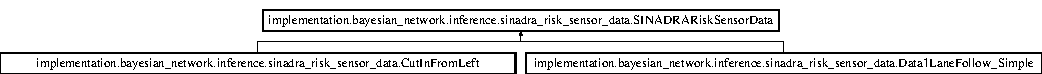
\includegraphics[height=0.663114cm]{classimplementation_1_1bayesian__network_1_1inference_1_1sinadra__risk__sensor__data_1_1_s_i_n_a_d_r_a_risk_sensor_data}
\end{center}
\end{figure}
\subsection*{Public Member Functions}
\begin{DoxyCompactItemize}
\item 
def \hyperlink{classimplementation_1_1bayesian__network_1_1inference_1_1sinadra__risk__sensor__data_1_1_s_i_n_a_d_r_a_risk_sensor_data_a554eb2647b96b3956764d60ecdec2425}{collect\+\_\+data\+\_\+from\+\_\+carla}
\end{DoxyCompactItemize}


\subsection{Detailed Description}
\begin{DoxyVerb}Input feature data class for Bayesian networks. Each Bayesian network shall have its own custom implementation
with its custom input features for situation-specific runtime updates.
\end{DoxyVerb}
 

\subsection{Member Function Documentation}
\mbox{\Hypertarget{classimplementation_1_1bayesian__network_1_1inference_1_1sinadra__risk__sensor__data_1_1_s_i_n_a_d_r_a_risk_sensor_data_a554eb2647b96b3956764d60ecdec2425}\label{classimplementation_1_1bayesian__network_1_1inference_1_1sinadra__risk__sensor__data_1_1_s_i_n_a_d_r_a_risk_sensor_data_a554eb2647b96b3956764d60ecdec2425}} 
\index{implementation\+::bayesian\+\_\+network\+::inference\+::sinadra\+\_\+risk\+\_\+sensor\+\_\+data\+::\+S\+I\+N\+A\+D\+R\+A\+Risk\+Sensor\+Data@{implementation\+::bayesian\+\_\+network\+::inference\+::sinadra\+\_\+risk\+\_\+sensor\+\_\+data\+::\+S\+I\+N\+A\+D\+R\+A\+Risk\+Sensor\+Data}!collect\+\_\+data\+\_\+from\+\_\+carla@{collect\+\_\+data\+\_\+from\+\_\+carla}}
\index{collect\+\_\+data\+\_\+from\+\_\+carla@{collect\+\_\+data\+\_\+from\+\_\+carla}!implementation\+::bayesian\+\_\+network\+::inference\+::sinadra\+\_\+risk\+\_\+sensor\+\_\+data\+::\+S\+I\+N\+A\+D\+R\+A\+Risk\+Sensor\+Data@{implementation\+::bayesian\+\_\+network\+::inference\+::sinadra\+\_\+risk\+\_\+sensor\+\_\+data\+::\+S\+I\+N\+A\+D\+R\+A\+Risk\+Sensor\+Data}}
\subsubsection{\texorpdfstring{collect\+\_\+data\+\_\+from\+\_\+carla()}{collect\_data\_from\_carla()}}
{\footnotesize\ttfamily def implementation.\+bayesian\+\_\+network.\+inference.\+sinadra\+\_\+risk\+\_\+sensor\+\_\+data.\+S\+I\+N\+A\+D\+R\+A\+Risk\+Sensor\+Data.\+collect\+\_\+data\+\_\+from\+\_\+carla (\begin{DoxyParamCaption}\item[{}]{self,  }\item[{}]{input\+\_\+feature\+\_\+data }\end{DoxyParamCaption})}



The documentation for this class was generated from the following file\+:\begin{DoxyCompactItemize}
\item 
implementation/bayesian\+\_\+network/inference/\hyperlink{sinadra__risk__sensor__data_8py}{sinadra\+\_\+risk\+\_\+sensor\+\_\+data.\+py}\end{DoxyCompactItemize}

\hypertarget{classimplementation_1_1actor__situation__class__detection_1_1situation__class_1_1_situation_class}{}\doxysection{implementation.\+actor\+\_\+situation\+\_\+class\+\_\+detection.\+situation\+\_\+class.\+Situation\+Class Class Reference}
\label{classimplementation_1_1actor__situation__class__detection_1_1situation__class_1_1_situation_class}\index{implementation.actor\_situation\_class\_detection.situation\_class.SituationClass@{implementation.actor\_situation\_class\_detection.situation\_class.SituationClass}}
Inheritance diagram for implementation.\+actor\+\_\+situation\+\_\+class\+\_\+detection.\+situation\+\_\+class.\+Situation\+Class\+:\begin{figure}[H]
\begin{center}
\leavevmode
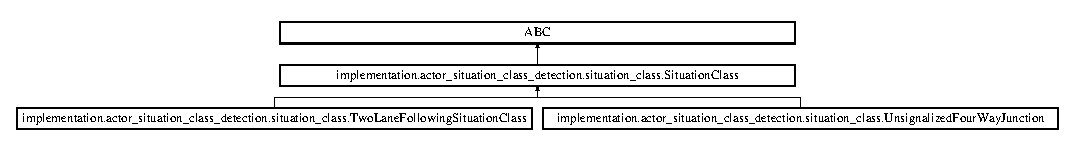
\includegraphics[height=1.510791cm]{classimplementation_1_1actor__situation__class__detection_1_1situation__class_1_1_situation_class}
\end{center}
\end{figure}
\doxysubsection*{Public Member Functions}
\begin{DoxyCompactItemize}
\item 
def \mbox{\hyperlink{classimplementation_1_1actor__situation__class__detection_1_1situation__class_1_1_situation_class_a51682d5b66a85fbf3283eb3e62d01a44}{\+\_\+\+\_\+init\+\_\+\+\_\+}} (self, str \mbox{\hyperlink{classimplementation_1_1actor__situation__class__detection_1_1situation__class_1_1_situation_class_a27d4d3259b8bb96107692e2b936ce801}{id}}, List\mbox{[}float\mbox{]} coordinates, \mbox{\hyperlink{classimplementation_1_1actor__situation__class__detection_1_1situation__class_1_1_situation_class_type}{Situation\+Class\+Type}} \mbox{\hyperlink{classimplementation_1_1actor__situation__class__detection_1_1situation__class_1_1_situation_class_a2782b467e701c72c8a445cfe7284f585}{situation\+\_\+type}})
\item 
def \mbox{\hyperlink{classimplementation_1_1actor__situation__class__detection_1_1situation__class_1_1_situation_class_a426da2947a5be8147db328181fdf9d45}{update\+\_\+wrapped\+\_\+actor\+\_\+association}} (self, \mbox{\hyperlink{classimplementation_1_1actor__situation__class__detection_1_1vehicle__actor__wrapper_1_1_vehicle_actor_wrapper}{Vehicle\+Actor\+Wrapper}} wrapped\+\_\+actor)
\item 
def \mbox{\hyperlink{classimplementation_1_1actor__situation__class__detection_1_1situation__class_1_1_situation_class_a78453f97c4d88f23beffccd6d6737e77}{clear\+\_\+actor\+\_\+associations}} (self)
\item 
def \mbox{\hyperlink{classimplementation_1_1actor__situation__class__detection_1_1situation__class_1_1_situation_class_a81e33d60e71cd9f46b5017c779d0a1a5}{print\+\_\+information}} (self, \mbox{\hyperlink{classimplementation_1_1actor__situation__class__detection_1_1vehicle__actor__wrapper_1_1_vehicle_actor_wrapper}{Vehicle\+Actor\+Wrapper}} wrapped\+\_\+actor)
\item 
def \mbox{\hyperlink{classimplementation_1_1actor__situation__class__detection_1_1situation__class_1_1_situation_class_aaba57b8546243184adbdabf500e22370}{set\+\_\+possible\+\_\+next\+\_\+situation\+\_\+classes\+\_\+by\+\_\+road\+\_\+segment\+\_\+end}} (self, Dict\mbox{[}\char`\"{}Road\+Segment\+End\char`\"{}, \char`\"{}\mbox{\hyperlink{classimplementation_1_1actor__situation__class__detection_1_1situation__class_1_1_situation_class}{Situation\+Class}}\char`\"{}\mbox{]} possible\+\_\+next\+\_\+situation\+\_\+classes\+\_\+by\+\_\+road\+\_\+segment\+\_\+end)
\item 
def \mbox{\hyperlink{classimplementation_1_1actor__situation__class__detection_1_1situation__class_1_1_situation_class_a503977f4c3f6e0b0350b266ac1a95b43}{set\+\_\+previous\+\_\+situation\+\_\+classes\+\_\+by\+\_\+road\+\_\+segment\+\_\+end}} (self, Dict\mbox{[}\char`\"{}Road\+Segment\+End\char`\"{}, \char`\"{}\mbox{\hyperlink{classimplementation_1_1actor__situation__class__detection_1_1situation__class_1_1_situation_class}{Situation\+Class}}\char`\"{}\mbox{]} previous\+\_\+situation\+\_\+classes\+\_\+by\+\_\+road\+\_\+segment\+\_\+end)
\item 
bool \mbox{\hyperlink{classimplementation_1_1actor__situation__class__detection_1_1situation__class_1_1_situation_class_a15317886621b68ae2d710ed7a10be803}{contains\+\_\+location}} (self, carla.\+Vector3D actor\+\_\+location)
\end{DoxyCompactItemize}
\doxysubsection*{Public Attributes}
\begin{DoxyCompactItemize}
\item 
\mbox{\hyperlink{classimplementation_1_1actor__situation__class__detection_1_1situation__class_1_1_situation_class_a2782b467e701c72c8a445cfe7284f585}{situation\+\_\+type}}
\item 
\mbox{\hyperlink{classimplementation_1_1actor__situation__class__detection_1_1situation__class_1_1_situation_class_a27d4d3259b8bb96107692e2b936ce801}{id}}
\item 
\mbox{\hyperlink{classimplementation_1_1actor__situation__class__detection_1_1situation__class_1_1_situation_class_af87990e3713cd82d257cd4b8ab5add6e}{wrapped\+\_\+actors\+\_\+in\+\_\+situation\+\_\+class}}
\item 
\mbox{\hyperlink{classimplementation_1_1actor__situation__class__detection_1_1situation__class_1_1_situation_class_a932a0f38eb6274f6d5f9812175f0365e}{possible\+\_\+next\+\_\+situation\+\_\+classes\+\_\+by\+\_\+road\+\_\+segment\+\_\+end}}
\item 
\mbox{\hyperlink{classimplementation_1_1actor__situation__class__detection_1_1situation__class_1_1_situation_class_add0a7a31f57b145a0c5af43ee596cb93}{previous\+\_\+situation\+\_\+classes\+\_\+by\+\_\+road\+\_\+segment\+\_\+end}}
\end{DoxyCompactItemize}


\doxysubsection{Detailed Description}
\begin{DoxyVerb}Super class of all specified situation classes. A situation class instance is defined for a certain area in a
town and knows which vehicles are currently in this area. A situation class can also be aware of which neighbor
situation classes are specified as next and previous situation classes for each road segment end of this
situation class

Attributes
----------
situation_type: SituationClassType
    Specifies the type of this situation class.
id: str
    Identifier of the situation class
wrapped_actors_in_situation_class: List[VehicleActorWrapper]
    A list of all Carla vehicles that are currently in the situation class wrapped into VehicleActorWrapper objects
possible_next_situation_classes_by_road_segment_end: Dict[RoadSegmentEnd, SituationClass]
    Dictionary of possible next situation classes categorized by a road segment end object as the dictionary key
previous_situation_classes_by_road_segment_end: Dict["RoadSegmentEnd", "SituationClass"]
    Dictionary of previous situation classes categorized by a road segment end object as the dictionary key
\end{DoxyVerb}
 

\doxysubsection{Constructor \& Destructor Documentation}
\mbox{\Hypertarget{classimplementation_1_1actor__situation__class__detection_1_1situation__class_1_1_situation_class_a51682d5b66a85fbf3283eb3e62d01a44}\label{classimplementation_1_1actor__situation__class__detection_1_1situation__class_1_1_situation_class_a51682d5b66a85fbf3283eb3e62d01a44}} 
\index{implementation.actor\_situation\_class\_detection.situation\_class.SituationClass@{implementation.actor\_situation\_class\_detection.situation\_class.SituationClass}!\_\_init\_\_@{\_\_init\_\_}}
\index{\_\_init\_\_@{\_\_init\_\_}!implementation.actor\_situation\_class\_detection.situation\_class.SituationClass@{implementation.actor\_situation\_class\_detection.situation\_class.SituationClass}}
\doxysubsubsection{\texorpdfstring{\_\_init\_\_()}{\_\_init\_\_()}}
{\footnotesize\ttfamily def implementation.\+actor\+\_\+situation\+\_\+class\+\_\+detection.\+situation\+\_\+class.\+Situation\+Class.\+\_\+\+\_\+init\+\_\+\+\_\+ (\begin{DoxyParamCaption}\item[{}]{self,  }\item[{str}]{id,  }\item[{List\mbox{[}float\mbox{]}}]{coordinates,  }\item[{\mbox{\hyperlink{classimplementation_1_1actor__situation__class__detection_1_1situation__class_1_1_situation_class_type}{Situation\+Class\+Type}}}]{situation\+\_\+type }\end{DoxyParamCaption})}

\begin{DoxyVerb}Constructor for the base class SituationClass

Parameters
----------
id: str
    Identifier string for situation class
coordinates: List[float]
    Corner point coordinates (X and Y coordinate) of the area the situation class shall be defined for.
situation_type: SituationClassType
    A SituationClassType object that specifies the type of this situation class.
\end{DoxyVerb}
 

\doxysubsection{Member Function Documentation}
\mbox{\Hypertarget{classimplementation_1_1actor__situation__class__detection_1_1situation__class_1_1_situation_class_a78453f97c4d88f23beffccd6d6737e77}\label{classimplementation_1_1actor__situation__class__detection_1_1situation__class_1_1_situation_class_a78453f97c4d88f23beffccd6d6737e77}} 
\index{implementation.actor\_situation\_class\_detection.situation\_class.SituationClass@{implementation.actor\_situation\_class\_detection.situation\_class.SituationClass}!clear\_actor\_associations@{clear\_actor\_associations}}
\index{clear\_actor\_associations@{clear\_actor\_associations}!implementation.actor\_situation\_class\_detection.situation\_class.SituationClass@{implementation.actor\_situation\_class\_detection.situation\_class.SituationClass}}
\doxysubsubsection{\texorpdfstring{clear\_actor\_associations()}{clear\_actor\_associations()}}
{\footnotesize\ttfamily def implementation.\+actor\+\_\+situation\+\_\+class\+\_\+detection.\+situation\+\_\+class.\+Situation\+Class.\+clear\+\_\+actor\+\_\+associations (\begin{DoxyParamCaption}\item[{}]{self }\end{DoxyParamCaption})}

\begin{DoxyVerb}Removes all associations to wrapped vehicle actors. This method is abstract and has to be implemented in the
specific situation class class definition, as each situation class could handle the vehicle association
differently.\end{DoxyVerb}
 

Reimplemented in \mbox{\hyperlink{classimplementation_1_1actor__situation__class__detection_1_1situation__class_1_1_unsignalized_four_way_junction_a0847bd9feb8f04f055599ac084c8228e}{implementation.\+actor\+\_\+situation\+\_\+class\+\_\+detection.\+situation\+\_\+class.\+Unsignalized\+Four\+Way\+Junction}}, and \mbox{\hyperlink{classimplementation_1_1actor__situation__class__detection_1_1situation__class_1_1_two_lane_following_situation_class_a12f727ba21c4b086d50738a3663da044}{implementation.\+actor\+\_\+situation\+\_\+class\+\_\+detection.\+situation\+\_\+class.\+Two\+Lane\+Following\+Situation\+Class}}.

\mbox{\Hypertarget{classimplementation_1_1actor__situation__class__detection_1_1situation__class_1_1_situation_class_a15317886621b68ae2d710ed7a10be803}\label{classimplementation_1_1actor__situation__class__detection_1_1situation__class_1_1_situation_class_a15317886621b68ae2d710ed7a10be803}} 
\index{implementation.actor\_situation\_class\_detection.situation\_class.SituationClass@{implementation.actor\_situation\_class\_detection.situation\_class.SituationClass}!contains\_location@{contains\_location}}
\index{contains\_location@{contains\_location}!implementation.actor\_situation\_class\_detection.situation\_class.SituationClass@{implementation.actor\_situation\_class\_detection.situation\_class.SituationClass}}
\doxysubsubsection{\texorpdfstring{contains\_location()}{contains\_location()}}
{\footnotesize\ttfamily  bool implementation.\+actor\+\_\+situation\+\_\+class\+\_\+detection.\+situation\+\_\+class.\+Situation\+Class.\+contains\+\_\+location (\begin{DoxyParamCaption}\item[{}]{self,  }\item[{carla.\+Vector3D}]{actor\+\_\+location }\end{DoxyParamCaption})}

\begin{DoxyVerb}Determines if given actor_location is within the area of this situation class. Therefore the
carla.Vector3D object is used to create a two dimensional point with the location's X and Y coordinates,
which is further used to check if its within the situation class' area.

Parameters
----------
actor_location: carla.Vector3D
    A carla.Vector3D object that represents the location that is checked if it's in the situation class' area.
Returns
-------
bool
    True if actor location is within situation class area.
    False if actor location is not within situation class area.
\end{DoxyVerb}
 \mbox{\Hypertarget{classimplementation_1_1actor__situation__class__detection_1_1situation__class_1_1_situation_class_a81e33d60e71cd9f46b5017c779d0a1a5}\label{classimplementation_1_1actor__situation__class__detection_1_1situation__class_1_1_situation_class_a81e33d60e71cd9f46b5017c779d0a1a5}} 
\index{implementation.actor\_situation\_class\_detection.situation\_class.SituationClass@{implementation.actor\_situation\_class\_detection.situation\_class.SituationClass}!print\_information@{print\_information}}
\index{print\_information@{print\_information}!implementation.actor\_situation\_class\_detection.situation\_class.SituationClass@{implementation.actor\_situation\_class\_detection.situation\_class.SituationClass}}
\doxysubsubsection{\texorpdfstring{print\_information()}{print\_information()}}
{\footnotesize\ttfamily def implementation.\+actor\+\_\+situation\+\_\+class\+\_\+detection.\+situation\+\_\+class.\+Situation\+Class.\+print\+\_\+information (\begin{DoxyParamCaption}\item[{}]{self,  }\item[{\mbox{\hyperlink{classimplementation_1_1actor__situation__class__detection_1_1vehicle__actor__wrapper_1_1_vehicle_actor_wrapper}{Vehicle\+Actor\+Wrapper}}}]{wrapped\+\_\+actor }\end{DoxyParamCaption})}

\begin{DoxyVerb}Prints information to the console. This method is abstract and has to be implemented in teh specific
situation class class definition for providing situation class type specific information. \end{DoxyVerb}
 

Reimplemented in \mbox{\hyperlink{classimplementation_1_1actor__situation__class__detection_1_1situation__class_1_1_two_lane_following_situation_class_ab4e14af65c524b3f5eb8266e14675487}{implementation.\+actor\+\_\+situation\+\_\+class\+\_\+detection.\+situation\+\_\+class.\+Two\+Lane\+Following\+Situation\+Class}}.

\mbox{\Hypertarget{classimplementation_1_1actor__situation__class__detection_1_1situation__class_1_1_situation_class_aaba57b8546243184adbdabf500e22370}\label{classimplementation_1_1actor__situation__class__detection_1_1situation__class_1_1_situation_class_aaba57b8546243184adbdabf500e22370}} 
\index{implementation.actor\_situation\_class\_detection.situation\_class.SituationClass@{implementation.actor\_situation\_class\_detection.situation\_class.SituationClass}!set\_possible\_next\_situation\_classes\_by\_road\_segment\_end@{set\_possible\_next\_situation\_classes\_by\_road\_segment\_end}}
\index{set\_possible\_next\_situation\_classes\_by\_road\_segment\_end@{set\_possible\_next\_situation\_classes\_by\_road\_segment\_end}!implementation.actor\_situation\_class\_detection.situation\_class.SituationClass@{implementation.actor\_situation\_class\_detection.situation\_class.SituationClass}}
\doxysubsubsection{\texorpdfstring{set\_possible\_next\_situation\_classes\_by\_road\_segment\_end()}{set\_possible\_next\_situation\_classes\_by\_road\_segment\_end()}}
{\footnotesize\ttfamily def implementation.\+actor\+\_\+situation\+\_\+class\+\_\+detection.\+situation\+\_\+class.\+Situation\+Class.\+set\+\_\+possible\+\_\+next\+\_\+situation\+\_\+classes\+\_\+by\+\_\+road\+\_\+segment\+\_\+end (\begin{DoxyParamCaption}\item[{}]{self,  }\item[{Dict\mbox{[}\char`\"{}Road\+Segment\+End\char`\"{}, \char`\"{}\mbox{\hyperlink{classimplementation_1_1actor__situation__class__detection_1_1situation__class_1_1_situation_class}{Situation\+Class}}\char`\"{}\mbox{]}}]{possible\+\_\+next\+\_\+situation\+\_\+classes\+\_\+by\+\_\+road\+\_\+segment\+\_\+end }\end{DoxyParamCaption})}

\begin{DoxyVerb}Sets the situations class public attribute possible_next_situation_classes_by_road_segment_end to passed
parameter value

Parameters
----------
possible_next_situation_classes_by_road_segment_end: Dict[RoadSegmentEnd, SituationClass]
    Dictionary of possible next situation classes categorized by a road segment end object as the dictionary key
\end{DoxyVerb}
 \mbox{\Hypertarget{classimplementation_1_1actor__situation__class__detection_1_1situation__class_1_1_situation_class_a503977f4c3f6e0b0350b266ac1a95b43}\label{classimplementation_1_1actor__situation__class__detection_1_1situation__class_1_1_situation_class_a503977f4c3f6e0b0350b266ac1a95b43}} 
\index{implementation.actor\_situation\_class\_detection.situation\_class.SituationClass@{implementation.actor\_situation\_class\_detection.situation\_class.SituationClass}!set\_previous\_situation\_classes\_by\_road\_segment\_end@{set\_previous\_situation\_classes\_by\_road\_segment\_end}}
\index{set\_previous\_situation\_classes\_by\_road\_segment\_end@{set\_previous\_situation\_classes\_by\_road\_segment\_end}!implementation.actor\_situation\_class\_detection.situation\_class.SituationClass@{implementation.actor\_situation\_class\_detection.situation\_class.SituationClass}}
\doxysubsubsection{\texorpdfstring{set\_previous\_situation\_classes\_by\_road\_segment\_end()}{set\_previous\_situation\_classes\_by\_road\_segment\_end()}}
{\footnotesize\ttfamily def implementation.\+actor\+\_\+situation\+\_\+class\+\_\+detection.\+situation\+\_\+class.\+Situation\+Class.\+set\+\_\+previous\+\_\+situation\+\_\+classes\+\_\+by\+\_\+road\+\_\+segment\+\_\+end (\begin{DoxyParamCaption}\item[{}]{self,  }\item[{Dict\mbox{[}\char`\"{}Road\+Segment\+End\char`\"{}, \char`\"{}\mbox{\hyperlink{classimplementation_1_1actor__situation__class__detection_1_1situation__class_1_1_situation_class}{Situation\+Class}}\char`\"{}\mbox{]}}]{previous\+\_\+situation\+\_\+classes\+\_\+by\+\_\+road\+\_\+segment\+\_\+end }\end{DoxyParamCaption})}

\begin{DoxyVerb}Sets the situations class public attribute previous_situation_classes_by_road_segment_end to passed
parameter value

Parameters
----------
previous_situation_classes_by_road_segment_end: Dict["RoadSegmentEnd", "SituationClass"]
    Dictionary of previous situation classes categorized by a road segment end object as the dictionary key
\end{DoxyVerb}
 \mbox{\Hypertarget{classimplementation_1_1actor__situation__class__detection_1_1situation__class_1_1_situation_class_a426da2947a5be8147db328181fdf9d45}\label{classimplementation_1_1actor__situation__class__detection_1_1situation__class_1_1_situation_class_a426da2947a5be8147db328181fdf9d45}} 
\index{implementation.actor\_situation\_class\_detection.situation\_class.SituationClass@{implementation.actor\_situation\_class\_detection.situation\_class.SituationClass}!update\_wrapped\_actor\_association@{update\_wrapped\_actor\_association}}
\index{update\_wrapped\_actor\_association@{update\_wrapped\_actor\_association}!implementation.actor\_situation\_class\_detection.situation\_class.SituationClass@{implementation.actor\_situation\_class\_detection.situation\_class.SituationClass}}
\doxysubsubsection{\texorpdfstring{update\_wrapped\_actor\_association()}{update\_wrapped\_actor\_association()}}
{\footnotesize\ttfamily def implementation.\+actor\+\_\+situation\+\_\+class\+\_\+detection.\+situation\+\_\+class.\+Situation\+Class.\+update\+\_\+wrapped\+\_\+actor\+\_\+association (\begin{DoxyParamCaption}\item[{}]{self,  }\item[{\mbox{\hyperlink{classimplementation_1_1actor__situation__class__detection_1_1vehicle__actor__wrapper_1_1_vehicle_actor_wrapper}{Vehicle\+Actor\+Wrapper}}}]{wrapped\+\_\+actor }\end{DoxyParamCaption})}

\begin{DoxyVerb}Associates the passed wrapped actor to this situation class. The association has to be implemented in the
specific situation class class definition, as each situation class could associate the wrapped actor to it in
a different way.

Parameters
----------
wrapped_actor: VehicleActorWrapper
    The carla vehicle actor wrapped into a VehicleActorWrapper object that shall be associated to the
    situation class.
\end{DoxyVerb}
 

Reimplemented in \mbox{\hyperlink{classimplementation_1_1actor__situation__class__detection_1_1situation__class_1_1_two_lane_following_situation_class_a2af23e4d2de43eb37f46f72300a4f5bd}{implementation.\+actor\+\_\+situation\+\_\+class\+\_\+detection.\+situation\+\_\+class.\+Two\+Lane\+Following\+Situation\+Class}}.



\doxysubsection{Member Data Documentation}
\mbox{\Hypertarget{classimplementation_1_1actor__situation__class__detection_1_1situation__class_1_1_situation_class_a27d4d3259b8bb96107692e2b936ce801}\label{classimplementation_1_1actor__situation__class__detection_1_1situation__class_1_1_situation_class_a27d4d3259b8bb96107692e2b936ce801}} 
\index{implementation.actor\_situation\_class\_detection.situation\_class.SituationClass@{implementation.actor\_situation\_class\_detection.situation\_class.SituationClass}!id@{id}}
\index{id@{id}!implementation.actor\_situation\_class\_detection.situation\_class.SituationClass@{implementation.actor\_situation\_class\_detection.situation\_class.SituationClass}}
\doxysubsubsection{\texorpdfstring{id}{id}}
{\footnotesize\ttfamily implementation.\+actor\+\_\+situation\+\_\+class\+\_\+detection.\+situation\+\_\+class.\+Situation\+Class.\+id}

\mbox{\Hypertarget{classimplementation_1_1actor__situation__class__detection_1_1situation__class_1_1_situation_class_a932a0f38eb6274f6d5f9812175f0365e}\label{classimplementation_1_1actor__situation__class__detection_1_1situation__class_1_1_situation_class_a932a0f38eb6274f6d5f9812175f0365e}} 
\index{implementation.actor\_situation\_class\_detection.situation\_class.SituationClass@{implementation.actor\_situation\_class\_detection.situation\_class.SituationClass}!possible\_next\_situation\_classes\_by\_road\_segment\_end@{possible\_next\_situation\_classes\_by\_road\_segment\_end}}
\index{possible\_next\_situation\_classes\_by\_road\_segment\_end@{possible\_next\_situation\_classes\_by\_road\_segment\_end}!implementation.actor\_situation\_class\_detection.situation\_class.SituationClass@{implementation.actor\_situation\_class\_detection.situation\_class.SituationClass}}
\doxysubsubsection{\texorpdfstring{possible\_next\_situation\_classes\_by\_road\_segment\_end}{possible\_next\_situation\_classes\_by\_road\_segment\_end}}
{\footnotesize\ttfamily implementation.\+actor\+\_\+situation\+\_\+class\+\_\+detection.\+situation\+\_\+class.\+Situation\+Class.\+possible\+\_\+next\+\_\+situation\+\_\+classes\+\_\+by\+\_\+road\+\_\+segment\+\_\+end}

\mbox{\Hypertarget{classimplementation_1_1actor__situation__class__detection_1_1situation__class_1_1_situation_class_add0a7a31f57b145a0c5af43ee596cb93}\label{classimplementation_1_1actor__situation__class__detection_1_1situation__class_1_1_situation_class_add0a7a31f57b145a0c5af43ee596cb93}} 
\index{implementation.actor\_situation\_class\_detection.situation\_class.SituationClass@{implementation.actor\_situation\_class\_detection.situation\_class.SituationClass}!previous\_situation\_classes\_by\_road\_segment\_end@{previous\_situation\_classes\_by\_road\_segment\_end}}
\index{previous\_situation\_classes\_by\_road\_segment\_end@{previous\_situation\_classes\_by\_road\_segment\_end}!implementation.actor\_situation\_class\_detection.situation\_class.SituationClass@{implementation.actor\_situation\_class\_detection.situation\_class.SituationClass}}
\doxysubsubsection{\texorpdfstring{previous\_situation\_classes\_by\_road\_segment\_end}{previous\_situation\_classes\_by\_road\_segment\_end}}
{\footnotesize\ttfamily implementation.\+actor\+\_\+situation\+\_\+class\+\_\+detection.\+situation\+\_\+class.\+Situation\+Class.\+previous\+\_\+situation\+\_\+classes\+\_\+by\+\_\+road\+\_\+segment\+\_\+end}

\mbox{\Hypertarget{classimplementation_1_1actor__situation__class__detection_1_1situation__class_1_1_situation_class_a2782b467e701c72c8a445cfe7284f585}\label{classimplementation_1_1actor__situation__class__detection_1_1situation__class_1_1_situation_class_a2782b467e701c72c8a445cfe7284f585}} 
\index{implementation.actor\_situation\_class\_detection.situation\_class.SituationClass@{implementation.actor\_situation\_class\_detection.situation\_class.SituationClass}!situation\_type@{situation\_type}}
\index{situation\_type@{situation\_type}!implementation.actor\_situation\_class\_detection.situation\_class.SituationClass@{implementation.actor\_situation\_class\_detection.situation\_class.SituationClass}}
\doxysubsubsection{\texorpdfstring{situation\_type}{situation\_type}}
{\footnotesize\ttfamily implementation.\+actor\+\_\+situation\+\_\+class\+\_\+detection.\+situation\+\_\+class.\+Situation\+Class.\+situation\+\_\+type}

\mbox{\Hypertarget{classimplementation_1_1actor__situation__class__detection_1_1situation__class_1_1_situation_class_af87990e3713cd82d257cd4b8ab5add6e}\label{classimplementation_1_1actor__situation__class__detection_1_1situation__class_1_1_situation_class_af87990e3713cd82d257cd4b8ab5add6e}} 
\index{implementation.actor\_situation\_class\_detection.situation\_class.SituationClass@{implementation.actor\_situation\_class\_detection.situation\_class.SituationClass}!wrapped\_actors\_in\_situation\_class@{wrapped\_actors\_in\_situation\_class}}
\index{wrapped\_actors\_in\_situation\_class@{wrapped\_actors\_in\_situation\_class}!implementation.actor\_situation\_class\_detection.situation\_class.SituationClass@{implementation.actor\_situation\_class\_detection.situation\_class.SituationClass}}
\doxysubsubsection{\texorpdfstring{wrapped\_actors\_in\_situation\_class}{wrapped\_actors\_in\_situation\_class}}
{\footnotesize\ttfamily implementation.\+actor\+\_\+situation\+\_\+class\+\_\+detection.\+situation\+\_\+class.\+Situation\+Class.\+wrapped\+\_\+actors\+\_\+in\+\_\+situation\+\_\+class}



The documentation for this class was generated from the following file\+:\begin{DoxyCompactItemize}
\item 
implementation/actor\+\_\+situation\+\_\+class\+\_\+detection/\mbox{\hyperlink{situation__class_8py}{situation\+\_\+class.\+py}}\end{DoxyCompactItemize}

\hypertarget{classimplementation_1_1actor__situation__class__detection_1_1situation__class_1_1_situation_class_stage}{}\doxysection{implementation.\+actor\+\_\+situation\+\_\+class\+\_\+detection.\+situation\+\_\+class.\+Situation\+Class\+Stage Class Reference}
\label{classimplementation_1_1actor__situation__class__detection_1_1situation__class_1_1_situation_class_stage}\index{implementation.actor\_situation\_class\_detection.situation\_class.SituationClassStage@{implementation.actor\_situation\_class\_detection.situation\_class.SituationClassStage}}
Inheritance diagram for implementation.\+actor\+\_\+situation\+\_\+class\+\_\+detection.\+situation\+\_\+class.\+Situation\+Class\+Stage\+:\begin{figure}[H]
\begin{center}
\leavevmode
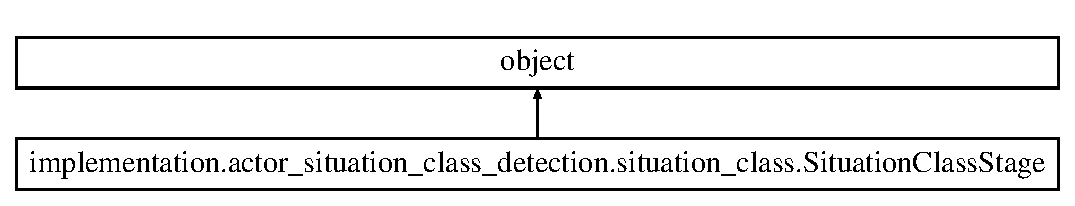
\includegraphics[height=2.000000cm]{classimplementation_1_1actor__situation__class__detection_1_1situation__class_1_1_situation_class_stage}
\end{center}
\end{figure}
\doxysubsection*{Public Member Functions}
\begin{DoxyCompactItemize}
\item 
def \mbox{\hyperlink{classimplementation_1_1actor__situation__class__detection_1_1situation__class_1_1_situation_class_stage_a4e80029b514cc3cd078fa5d3fa638394}{\+\_\+\+\_\+init\+\_\+\+\_\+}} (self, \mbox{\hyperlink{classimplementation_1_1actor__situation__class__detection_1_1situation__class_1_1_situation_class_type}{Situation\+Class\+Type}} situation\+\_\+class\+\_\+stage\+\_\+type, List\mbox{[}\char`\"{}Situation\+Class\+Stage\char`\"{}\mbox{]} previous\+\_\+stages, List\mbox{[}\char`\"{}Situation\+Class\+Stage\char`\"{}\mbox{]} next\+\_\+stages)
\end{DoxyCompactItemize}
\doxysubsection*{Public Attributes}
\begin{DoxyCompactItemize}
\item 
\mbox{\hyperlink{classimplementation_1_1actor__situation__class__detection_1_1situation__class_1_1_situation_class_stage_a2739ff793de57b513621a5bba3ced6eb}{type}}
\item 
\mbox{\hyperlink{classimplementation_1_1actor__situation__class__detection_1_1situation__class_1_1_situation_class_stage_a0cff48353fee8813eb25d53337f851b3}{previous\+\_\+stages}}
\item 
\mbox{\hyperlink{classimplementation_1_1actor__situation__class__detection_1_1situation__class_1_1_situation_class_stage_af5f9b64b63ea973eccea97393dc33f3c}{next\+\_\+stages}}
\end{DoxyCompactItemize}


\doxysubsection{Detailed Description}
\begin{DoxyVerb}Can be used used to further divide a situation class into several stages, where each of the stage knows the
previous and next stages. \end{DoxyVerb}
 

\doxysubsection{Constructor \& Destructor Documentation}
\mbox{\Hypertarget{classimplementation_1_1actor__situation__class__detection_1_1situation__class_1_1_situation_class_stage_a4e80029b514cc3cd078fa5d3fa638394}\label{classimplementation_1_1actor__situation__class__detection_1_1situation__class_1_1_situation_class_stage_a4e80029b514cc3cd078fa5d3fa638394}} 
\index{implementation.actor\_situation\_class\_detection.situation\_class.SituationClassStage@{implementation.actor\_situation\_class\_detection.situation\_class.SituationClassStage}!\_\_init\_\_@{\_\_init\_\_}}
\index{\_\_init\_\_@{\_\_init\_\_}!implementation.actor\_situation\_class\_detection.situation\_class.SituationClassStage@{implementation.actor\_situation\_class\_detection.situation\_class.SituationClassStage}}
\doxysubsubsection{\texorpdfstring{\_\_init\_\_()}{\_\_init\_\_()}}
{\footnotesize\ttfamily def implementation.\+actor\+\_\+situation\+\_\+class\+\_\+detection.\+situation\+\_\+class.\+Situation\+Class\+Stage.\+\_\+\+\_\+init\+\_\+\+\_\+ (\begin{DoxyParamCaption}\item[{}]{self,  }\item[{\mbox{\hyperlink{classimplementation_1_1actor__situation__class__detection_1_1situation__class_1_1_situation_class_type}{Situation\+Class\+Type}}}]{situation\+\_\+class\+\_\+stage\+\_\+type,  }\item[{List\mbox{[}\char`\"{}Situation\+Class\+Stage\char`\"{}\mbox{]}}]{previous\+\_\+stages,  }\item[{List\mbox{[}\char`\"{}Situation\+Class\+Stage\char`\"{}\mbox{]}}]{next\+\_\+stages }\end{DoxyParamCaption})}



\doxysubsection{Member Data Documentation}
\mbox{\Hypertarget{classimplementation_1_1actor__situation__class__detection_1_1situation__class_1_1_situation_class_stage_af5f9b64b63ea973eccea97393dc33f3c}\label{classimplementation_1_1actor__situation__class__detection_1_1situation__class_1_1_situation_class_stage_af5f9b64b63ea973eccea97393dc33f3c}} 
\index{implementation.actor\_situation\_class\_detection.situation\_class.SituationClassStage@{implementation.actor\_situation\_class\_detection.situation\_class.SituationClassStage}!next\_stages@{next\_stages}}
\index{next\_stages@{next\_stages}!implementation.actor\_situation\_class\_detection.situation\_class.SituationClassStage@{implementation.actor\_situation\_class\_detection.situation\_class.SituationClassStage}}
\doxysubsubsection{\texorpdfstring{next\_stages}{next\_stages}}
{\footnotesize\ttfamily implementation.\+actor\+\_\+situation\+\_\+class\+\_\+detection.\+situation\+\_\+class.\+Situation\+Class\+Stage.\+next\+\_\+stages}

\mbox{\Hypertarget{classimplementation_1_1actor__situation__class__detection_1_1situation__class_1_1_situation_class_stage_a0cff48353fee8813eb25d53337f851b3}\label{classimplementation_1_1actor__situation__class__detection_1_1situation__class_1_1_situation_class_stage_a0cff48353fee8813eb25d53337f851b3}} 
\index{implementation.actor\_situation\_class\_detection.situation\_class.SituationClassStage@{implementation.actor\_situation\_class\_detection.situation\_class.SituationClassStage}!previous\_stages@{previous\_stages}}
\index{previous\_stages@{previous\_stages}!implementation.actor\_situation\_class\_detection.situation\_class.SituationClassStage@{implementation.actor\_situation\_class\_detection.situation\_class.SituationClassStage}}
\doxysubsubsection{\texorpdfstring{previous\_stages}{previous\_stages}}
{\footnotesize\ttfamily implementation.\+actor\+\_\+situation\+\_\+class\+\_\+detection.\+situation\+\_\+class.\+Situation\+Class\+Stage.\+previous\+\_\+stages}

\mbox{\Hypertarget{classimplementation_1_1actor__situation__class__detection_1_1situation__class_1_1_situation_class_stage_a2739ff793de57b513621a5bba3ced6eb}\label{classimplementation_1_1actor__situation__class__detection_1_1situation__class_1_1_situation_class_stage_a2739ff793de57b513621a5bba3ced6eb}} 
\index{implementation.actor\_situation\_class\_detection.situation\_class.SituationClassStage@{implementation.actor\_situation\_class\_detection.situation\_class.SituationClassStage}!type@{type}}
\index{type@{type}!implementation.actor\_situation\_class\_detection.situation\_class.SituationClassStage@{implementation.actor\_situation\_class\_detection.situation\_class.SituationClassStage}}
\doxysubsubsection{\texorpdfstring{type}{type}}
{\footnotesize\ttfamily implementation.\+actor\+\_\+situation\+\_\+class\+\_\+detection.\+situation\+\_\+class.\+Situation\+Class\+Stage.\+type}



The documentation for this class was generated from the following file\+:\begin{DoxyCompactItemize}
\item 
implementation/actor\+\_\+situation\+\_\+class\+\_\+detection/\mbox{\hyperlink{situation__class_8py}{situation\+\_\+class.\+py}}\end{DoxyCompactItemize}

\hypertarget{classimplementation_1_1actor__situation__class__detection_1_1situation__class_1_1_situation_class_stage_types}{}\section{implementation.\+actor\+\_\+situation\+\_\+class\+\_\+detection.\+situation\+\_\+class.\+Situation\+Class\+Stage\+Types Class Reference}
\label{classimplementation_1_1actor__situation__class__detection_1_1situation__class_1_1_situation_class_stage_types}\index{implementation.\+actor\+\_\+situation\+\_\+class\+\_\+detection.\+situation\+\_\+class.\+Situation\+Class\+Stage\+Types@{implementation.\+actor\+\_\+situation\+\_\+class\+\_\+detection.\+situation\+\_\+class.\+Situation\+Class\+Stage\+Types}}
Inheritance diagram for implementation.\+actor\+\_\+situation\+\_\+class\+\_\+detection.\+situation\+\_\+class.\+Situation\+Class\+Stage\+Types\+:\begin{figure}[H]
\begin{center}
\leavevmode
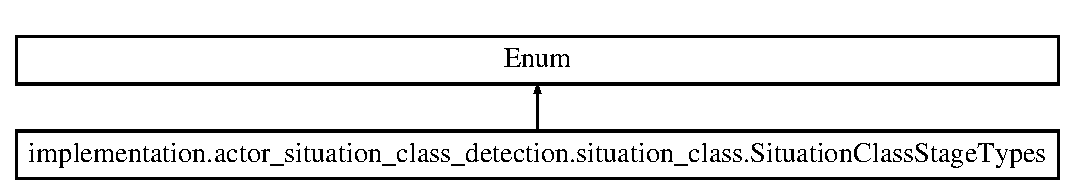
\includegraphics[height=2.000000cm]{classimplementation_1_1actor__situation__class__detection_1_1situation__class_1_1_situation_class_stage_types}
\end{center}
\end{figure}
\subsection*{Static Public Attributes}
\begin{DoxyCompactItemize}
\item 
int \hyperlink{classimplementation_1_1actor__situation__class__detection_1_1situation__class_1_1_situation_class_stage_types_a66dc0c8e325fc64191fa40103932e0c4}{E\+N\+T\+E\+R\+\_\+\+S\+I\+T\+U\+A\+T\+I\+O\+N\+\_\+\+C\+L\+A\+SS} = 1
\item 
int \hyperlink{classimplementation_1_1actor__situation__class__detection_1_1situation__class_1_1_situation_class_stage_types_a610c5162811196c8b8edab00507efe92}{D\+E\+F\+A\+U\+L\+T\+\_\+\+S\+T\+A\+GE} = 2
\item 
int \hyperlink{classimplementation_1_1actor__situation__class__detection_1_1situation__class_1_1_situation_class_stage_types_aa72493675b58b32a7803b85abd50d57c}{L\+E\+A\+V\+E\+\_\+\+S\+I\+T\+U\+A\+T\+I\+O\+N\+\_\+\+C\+L\+A\+SS} = 3
\item 
int \hyperlink{classimplementation_1_1actor__situation__class__detection_1_1situation__class_1_1_situation_class_stage_types_afe10604ad2d9f28a934e625a24fb707d}{N\+O\+NE} = 4
\end{DoxyCompactItemize}


\subsection{Member Data Documentation}
\mbox{\Hypertarget{classimplementation_1_1actor__situation__class__detection_1_1situation__class_1_1_situation_class_stage_types_a610c5162811196c8b8edab00507efe92}\label{classimplementation_1_1actor__situation__class__detection_1_1situation__class_1_1_situation_class_stage_types_a610c5162811196c8b8edab00507efe92}} 
\index{implementation\+::actor\+\_\+situation\+\_\+class\+\_\+detection\+::situation\+\_\+class\+::\+Situation\+Class\+Stage\+Types@{implementation\+::actor\+\_\+situation\+\_\+class\+\_\+detection\+::situation\+\_\+class\+::\+Situation\+Class\+Stage\+Types}!D\+E\+F\+A\+U\+L\+T\+\_\+\+S\+T\+A\+GE@{D\+E\+F\+A\+U\+L\+T\+\_\+\+S\+T\+A\+GE}}
\index{D\+E\+F\+A\+U\+L\+T\+\_\+\+S\+T\+A\+GE@{D\+E\+F\+A\+U\+L\+T\+\_\+\+S\+T\+A\+GE}!implementation\+::actor\+\_\+situation\+\_\+class\+\_\+detection\+::situation\+\_\+class\+::\+Situation\+Class\+Stage\+Types@{implementation\+::actor\+\_\+situation\+\_\+class\+\_\+detection\+::situation\+\_\+class\+::\+Situation\+Class\+Stage\+Types}}
\subsubsection{\texorpdfstring{D\+E\+F\+A\+U\+L\+T\+\_\+\+S\+T\+A\+GE}{DEFAULT\_STAGE}}
{\footnotesize\ttfamily int implementation.\+actor\+\_\+situation\+\_\+class\+\_\+detection.\+situation\+\_\+class.\+Situation\+Class\+Stage\+Types.\+D\+E\+F\+A\+U\+L\+T\+\_\+\+S\+T\+A\+GE = 2\hspace{0.3cm}{\ttfamily [static]}}

\mbox{\Hypertarget{classimplementation_1_1actor__situation__class__detection_1_1situation__class_1_1_situation_class_stage_types_a66dc0c8e325fc64191fa40103932e0c4}\label{classimplementation_1_1actor__situation__class__detection_1_1situation__class_1_1_situation_class_stage_types_a66dc0c8e325fc64191fa40103932e0c4}} 
\index{implementation\+::actor\+\_\+situation\+\_\+class\+\_\+detection\+::situation\+\_\+class\+::\+Situation\+Class\+Stage\+Types@{implementation\+::actor\+\_\+situation\+\_\+class\+\_\+detection\+::situation\+\_\+class\+::\+Situation\+Class\+Stage\+Types}!E\+N\+T\+E\+R\+\_\+\+S\+I\+T\+U\+A\+T\+I\+O\+N\+\_\+\+C\+L\+A\+SS@{E\+N\+T\+E\+R\+\_\+\+S\+I\+T\+U\+A\+T\+I\+O\+N\+\_\+\+C\+L\+A\+SS}}
\index{E\+N\+T\+E\+R\+\_\+\+S\+I\+T\+U\+A\+T\+I\+O\+N\+\_\+\+C\+L\+A\+SS@{E\+N\+T\+E\+R\+\_\+\+S\+I\+T\+U\+A\+T\+I\+O\+N\+\_\+\+C\+L\+A\+SS}!implementation\+::actor\+\_\+situation\+\_\+class\+\_\+detection\+::situation\+\_\+class\+::\+Situation\+Class\+Stage\+Types@{implementation\+::actor\+\_\+situation\+\_\+class\+\_\+detection\+::situation\+\_\+class\+::\+Situation\+Class\+Stage\+Types}}
\subsubsection{\texorpdfstring{E\+N\+T\+E\+R\+\_\+\+S\+I\+T\+U\+A\+T\+I\+O\+N\+\_\+\+C\+L\+A\+SS}{ENTER\_SITUATION\_CLASS}}
{\footnotesize\ttfamily int implementation.\+actor\+\_\+situation\+\_\+class\+\_\+detection.\+situation\+\_\+class.\+Situation\+Class\+Stage\+Types.\+E\+N\+T\+E\+R\+\_\+\+S\+I\+T\+U\+A\+T\+I\+O\+N\+\_\+\+C\+L\+A\+SS = 1\hspace{0.3cm}{\ttfamily [static]}}

\mbox{\Hypertarget{classimplementation_1_1actor__situation__class__detection_1_1situation__class_1_1_situation_class_stage_types_aa72493675b58b32a7803b85abd50d57c}\label{classimplementation_1_1actor__situation__class__detection_1_1situation__class_1_1_situation_class_stage_types_aa72493675b58b32a7803b85abd50d57c}} 
\index{implementation\+::actor\+\_\+situation\+\_\+class\+\_\+detection\+::situation\+\_\+class\+::\+Situation\+Class\+Stage\+Types@{implementation\+::actor\+\_\+situation\+\_\+class\+\_\+detection\+::situation\+\_\+class\+::\+Situation\+Class\+Stage\+Types}!L\+E\+A\+V\+E\+\_\+\+S\+I\+T\+U\+A\+T\+I\+O\+N\+\_\+\+C\+L\+A\+SS@{L\+E\+A\+V\+E\+\_\+\+S\+I\+T\+U\+A\+T\+I\+O\+N\+\_\+\+C\+L\+A\+SS}}
\index{L\+E\+A\+V\+E\+\_\+\+S\+I\+T\+U\+A\+T\+I\+O\+N\+\_\+\+C\+L\+A\+SS@{L\+E\+A\+V\+E\+\_\+\+S\+I\+T\+U\+A\+T\+I\+O\+N\+\_\+\+C\+L\+A\+SS}!implementation\+::actor\+\_\+situation\+\_\+class\+\_\+detection\+::situation\+\_\+class\+::\+Situation\+Class\+Stage\+Types@{implementation\+::actor\+\_\+situation\+\_\+class\+\_\+detection\+::situation\+\_\+class\+::\+Situation\+Class\+Stage\+Types}}
\subsubsection{\texorpdfstring{L\+E\+A\+V\+E\+\_\+\+S\+I\+T\+U\+A\+T\+I\+O\+N\+\_\+\+C\+L\+A\+SS}{LEAVE\_SITUATION\_CLASS}}
{\footnotesize\ttfamily int implementation.\+actor\+\_\+situation\+\_\+class\+\_\+detection.\+situation\+\_\+class.\+Situation\+Class\+Stage\+Types.\+L\+E\+A\+V\+E\+\_\+\+S\+I\+T\+U\+A\+T\+I\+O\+N\+\_\+\+C\+L\+A\+SS = 3\hspace{0.3cm}{\ttfamily [static]}}

\mbox{\Hypertarget{classimplementation_1_1actor__situation__class__detection_1_1situation__class_1_1_situation_class_stage_types_afe10604ad2d9f28a934e625a24fb707d}\label{classimplementation_1_1actor__situation__class__detection_1_1situation__class_1_1_situation_class_stage_types_afe10604ad2d9f28a934e625a24fb707d}} 
\index{implementation\+::actor\+\_\+situation\+\_\+class\+\_\+detection\+::situation\+\_\+class\+::\+Situation\+Class\+Stage\+Types@{implementation\+::actor\+\_\+situation\+\_\+class\+\_\+detection\+::situation\+\_\+class\+::\+Situation\+Class\+Stage\+Types}!N\+O\+NE@{N\+O\+NE}}
\index{N\+O\+NE@{N\+O\+NE}!implementation\+::actor\+\_\+situation\+\_\+class\+\_\+detection\+::situation\+\_\+class\+::\+Situation\+Class\+Stage\+Types@{implementation\+::actor\+\_\+situation\+\_\+class\+\_\+detection\+::situation\+\_\+class\+::\+Situation\+Class\+Stage\+Types}}
\subsubsection{\texorpdfstring{N\+O\+NE}{NONE}}
{\footnotesize\ttfamily int implementation.\+actor\+\_\+situation\+\_\+class\+\_\+detection.\+situation\+\_\+class.\+Situation\+Class\+Stage\+Types.\+N\+O\+NE = 4\hspace{0.3cm}{\ttfamily [static]}}



The documentation for this class was generated from the following file\+:\begin{DoxyCompactItemize}
\item 
implementation/actor\+\_\+situation\+\_\+class\+\_\+detection/\hyperlink{situation__class_8py}{situation\+\_\+class.\+py}\end{DoxyCompactItemize}

\hypertarget{classimplementation_1_1actor__situation__class__detection_1_1situation__class__state__machine_1_1_situation_class_state_machine}{}\section{implementation.\+actor\+\_\+situation\+\_\+class\+\_\+detection.\+situation\+\_\+class\+\_\+state\+\_\+machine.\+Situation\+Class\+State\+Machine Class Reference}
\label{classimplementation_1_1actor__situation__class__detection_1_1situation__class__state__machine_1_1_situation_class_state_machine}\index{implementation.\+actor\+\_\+situation\+\_\+class\+\_\+detection.\+situation\+\_\+class\+\_\+state\+\_\+machine.\+Situation\+Class\+State\+Machine@{implementation.\+actor\+\_\+situation\+\_\+class\+\_\+detection.\+situation\+\_\+class\+\_\+state\+\_\+machine.\+Situation\+Class\+State\+Machine}}
Inheritance diagram for implementation.\+actor\+\_\+situation\+\_\+class\+\_\+detection.\+situation\+\_\+class\+\_\+state\+\_\+machine.\+Situation\+Class\+State\+Machine\+:\begin{figure}[H]
\begin{center}
\leavevmode
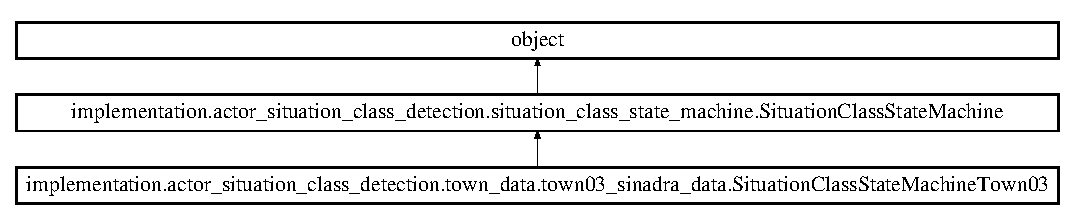
\includegraphics[height=2.503726cm]{classimplementation_1_1actor__situation__class__detection_1_1situation__class__state__machine_1_1_situation_class_state_machine}
\end{center}
\end{figure}
\subsection*{Public Member Functions}
\begin{DoxyCompactItemize}
\item 
def \hyperlink{classimplementation_1_1actor__situation__class__detection_1_1situation__class__state__machine_1_1_situation_class_state_machine_ae25ddb59e6a7d8a1ebfdd1e1441b5755}{\+\_\+\+\_\+init\+\_\+\+\_\+}
\item 
def \hyperlink{classimplementation_1_1actor__situation__class__detection_1_1situation__class__state__machine_1_1_situation_class_state_machine_ad6e1f4d300138b8c8d1a092bf1628b49}{clear\+\_\+actor\+\_\+associations\+\_\+from\+\_\+situation\+\_\+classes} (self)
\item 
def \hyperlink{classimplementation_1_1actor__situation__class__detection_1_1situation__class__state__machine_1_1_situation_class_state_machine_ab1271848fb25a8644f34b209d4ac9ed6}{update\+\_\+situation\+\_\+classes}
\item 
def \hyperlink{classimplementation_1_1actor__situation__class__detection_1_1situation__class__state__machine_1_1_situation_class_state_machine_a7a4a9a103a8526903fb4912a224b7cdd}{get\+\_\+hero\+\_\+situation\+\_\+class} (self)
\end{DoxyCompactItemize}
\subsection*{Public Attributes}
\begin{DoxyCompactItemize}
\item 
\hyperlink{classimplementation_1_1actor__situation__class__detection_1_1situation__class__state__machine_1_1_situation_class_state_machine_aa4eb1ddf0aa9f37f77c1bb3453b36161}{situation\+\_\+classes}
\item 
\hyperlink{classimplementation_1_1actor__situation__class__detection_1_1situation__class__state__machine_1_1_situation_class_state_machine_ab028cc98852fbcc54f37c51c1fc7128d}{ego\+\_\+situation\+\_\+class}
\end{DoxyCompactItemize}


\subsection{Detailed Description}
\begin{DoxyVerb}State machine class that contains all existing situation classes for a town. It provides methods updating the
situation classes regarding their actor associations, for clearing the already set actor associations from
situation classes and for determining the situation class the hero vehicle is currently in
\end{DoxyVerb}
 

\subsection{Constructor \& Destructor Documentation}
\mbox{\Hypertarget{classimplementation_1_1actor__situation__class__detection_1_1situation__class__state__machine_1_1_situation_class_state_machine_ae25ddb59e6a7d8a1ebfdd1e1441b5755}\label{classimplementation_1_1actor__situation__class__detection_1_1situation__class__state__machine_1_1_situation_class_state_machine_ae25ddb59e6a7d8a1ebfdd1e1441b5755}} 
\index{implementation\+::actor\+\_\+situation\+\_\+class\+\_\+detection\+::situation\+\_\+class\+\_\+state\+\_\+machine\+::\+Situation\+Class\+State\+Machine@{implementation\+::actor\+\_\+situation\+\_\+class\+\_\+detection\+::situation\+\_\+class\+\_\+state\+\_\+machine\+::\+Situation\+Class\+State\+Machine}!\+\_\+\+\_\+init\+\_\+\+\_\+@{\+\_\+\+\_\+init\+\_\+\+\_\+}}
\index{\+\_\+\+\_\+init\+\_\+\+\_\+@{\+\_\+\+\_\+init\+\_\+\+\_\+}!implementation\+::actor\+\_\+situation\+\_\+class\+\_\+detection\+::situation\+\_\+class\+\_\+state\+\_\+machine\+::\+Situation\+Class\+State\+Machine@{implementation\+::actor\+\_\+situation\+\_\+class\+\_\+detection\+::situation\+\_\+class\+\_\+state\+\_\+machine\+::\+Situation\+Class\+State\+Machine}}
\subsubsection{\texorpdfstring{\+\_\+\+\_\+init\+\_\+\+\_\+()}{\_\_init\_\_()}}
{\footnotesize\ttfamily def implementation.\+actor\+\_\+situation\+\_\+class\+\_\+detection.\+situation\+\_\+class\+\_\+state\+\_\+machine.\+Situation\+Class\+State\+Machine.\+\_\+\+\_\+init\+\_\+\+\_\+ (\begin{DoxyParamCaption}\item[{}]{self,  }\item[{}]{situation\+\_\+classes }\end{DoxyParamCaption})}



\subsection{Member Function Documentation}
\mbox{\Hypertarget{classimplementation_1_1actor__situation__class__detection_1_1situation__class__state__machine_1_1_situation_class_state_machine_ad6e1f4d300138b8c8d1a092bf1628b49}\label{classimplementation_1_1actor__situation__class__detection_1_1situation__class__state__machine_1_1_situation_class_state_machine_ad6e1f4d300138b8c8d1a092bf1628b49}} 
\index{implementation\+::actor\+\_\+situation\+\_\+class\+\_\+detection\+::situation\+\_\+class\+\_\+state\+\_\+machine\+::\+Situation\+Class\+State\+Machine@{implementation\+::actor\+\_\+situation\+\_\+class\+\_\+detection\+::situation\+\_\+class\+\_\+state\+\_\+machine\+::\+Situation\+Class\+State\+Machine}!clear\+\_\+actor\+\_\+associations\+\_\+from\+\_\+situation\+\_\+classes@{clear\+\_\+actor\+\_\+associations\+\_\+from\+\_\+situation\+\_\+classes}}
\index{clear\+\_\+actor\+\_\+associations\+\_\+from\+\_\+situation\+\_\+classes@{clear\+\_\+actor\+\_\+associations\+\_\+from\+\_\+situation\+\_\+classes}!implementation\+::actor\+\_\+situation\+\_\+class\+\_\+detection\+::situation\+\_\+class\+\_\+state\+\_\+machine\+::\+Situation\+Class\+State\+Machine@{implementation\+::actor\+\_\+situation\+\_\+class\+\_\+detection\+::situation\+\_\+class\+\_\+state\+\_\+machine\+::\+Situation\+Class\+State\+Machine}}
\subsubsection{\texorpdfstring{clear\+\_\+actor\+\_\+associations\+\_\+from\+\_\+situation\+\_\+classes()}{clear\_actor\_associations\_from\_situation\_classes()}}
{\footnotesize\ttfamily def implementation.\+actor\+\_\+situation\+\_\+class\+\_\+detection.\+situation\+\_\+class\+\_\+state\+\_\+machine.\+Situation\+Class\+State\+Machine.\+clear\+\_\+actor\+\_\+associations\+\_\+from\+\_\+situation\+\_\+classes (\begin{DoxyParamCaption}\item[{}]{self }\end{DoxyParamCaption})}

\begin{DoxyVerb}Method to remove all actors from situation class objects.\end{DoxyVerb}
 \mbox{\Hypertarget{classimplementation_1_1actor__situation__class__detection_1_1situation__class__state__machine_1_1_situation_class_state_machine_a7a4a9a103a8526903fb4912a224b7cdd}\label{classimplementation_1_1actor__situation__class__detection_1_1situation__class__state__machine_1_1_situation_class_state_machine_a7a4a9a103a8526903fb4912a224b7cdd}} 
\index{implementation\+::actor\+\_\+situation\+\_\+class\+\_\+detection\+::situation\+\_\+class\+\_\+state\+\_\+machine\+::\+Situation\+Class\+State\+Machine@{implementation\+::actor\+\_\+situation\+\_\+class\+\_\+detection\+::situation\+\_\+class\+\_\+state\+\_\+machine\+::\+Situation\+Class\+State\+Machine}!get\+\_\+hero\+\_\+situation\+\_\+class@{get\+\_\+hero\+\_\+situation\+\_\+class}}
\index{get\+\_\+hero\+\_\+situation\+\_\+class@{get\+\_\+hero\+\_\+situation\+\_\+class}!implementation\+::actor\+\_\+situation\+\_\+class\+\_\+detection\+::situation\+\_\+class\+\_\+state\+\_\+machine\+::\+Situation\+Class\+State\+Machine@{implementation\+::actor\+\_\+situation\+\_\+class\+\_\+detection\+::situation\+\_\+class\+\_\+state\+\_\+machine\+::\+Situation\+Class\+State\+Machine}}
\subsubsection{\texorpdfstring{get\+\_\+hero\+\_\+situation\+\_\+class()}{get\_hero\_situation\_class()}}
{\footnotesize\ttfamily def implementation.\+actor\+\_\+situation\+\_\+class\+\_\+detection.\+situation\+\_\+class\+\_\+state\+\_\+machine.\+Situation\+Class\+State\+Machine.\+get\+\_\+hero\+\_\+situation\+\_\+class (\begin{DoxyParamCaption}\item[{}]{self,  }\item[{}]{Optional,  }\item[{}]{Situation\+Class }\end{DoxyParamCaption})}

\begin{DoxyVerb}Retrieves the situation class the hero vehicle is currently in.

Returns
-------
SituationClass object, which the hero vehicle is currently allocated to. If hero vehicle can not be found in any
situation class, None is returned instead.
\end{DoxyVerb}
 \mbox{\Hypertarget{classimplementation_1_1actor__situation__class__detection_1_1situation__class__state__machine_1_1_situation_class_state_machine_ab1271848fb25a8644f34b209d4ac9ed6}\label{classimplementation_1_1actor__situation__class__detection_1_1situation__class__state__machine_1_1_situation_class_state_machine_ab1271848fb25a8644f34b209d4ac9ed6}} 
\index{implementation\+::actor\+\_\+situation\+\_\+class\+\_\+detection\+::situation\+\_\+class\+\_\+state\+\_\+machine\+::\+Situation\+Class\+State\+Machine@{implementation\+::actor\+\_\+situation\+\_\+class\+\_\+detection\+::situation\+\_\+class\+\_\+state\+\_\+machine\+::\+Situation\+Class\+State\+Machine}!update\+\_\+situation\+\_\+classes@{update\+\_\+situation\+\_\+classes}}
\index{update\+\_\+situation\+\_\+classes@{update\+\_\+situation\+\_\+classes}!implementation\+::actor\+\_\+situation\+\_\+class\+\_\+detection\+::situation\+\_\+class\+\_\+state\+\_\+machine\+::\+Situation\+Class\+State\+Machine@{implementation\+::actor\+\_\+situation\+\_\+class\+\_\+detection\+::situation\+\_\+class\+\_\+state\+\_\+machine\+::\+Situation\+Class\+State\+Machine}}
\subsubsection{\texorpdfstring{update\+\_\+situation\+\_\+classes()}{update\_situation\_classes()}}
{\footnotesize\ttfamily def implementation.\+actor\+\_\+situation\+\_\+class\+\_\+detection.\+situation\+\_\+class\+\_\+state\+\_\+machine.\+Situation\+Class\+State\+Machine.\+update\+\_\+situation\+\_\+classes (\begin{DoxyParamCaption}\item[{}]{self,  }\item[{}]{vehicles }\end{DoxyParamCaption})}



\subsection{Member Data Documentation}
\mbox{\Hypertarget{classimplementation_1_1actor__situation__class__detection_1_1situation__class__state__machine_1_1_situation_class_state_machine_ab028cc98852fbcc54f37c51c1fc7128d}\label{classimplementation_1_1actor__situation__class__detection_1_1situation__class__state__machine_1_1_situation_class_state_machine_ab028cc98852fbcc54f37c51c1fc7128d}} 
\index{implementation\+::actor\+\_\+situation\+\_\+class\+\_\+detection\+::situation\+\_\+class\+\_\+state\+\_\+machine\+::\+Situation\+Class\+State\+Machine@{implementation\+::actor\+\_\+situation\+\_\+class\+\_\+detection\+::situation\+\_\+class\+\_\+state\+\_\+machine\+::\+Situation\+Class\+State\+Machine}!ego\+\_\+situation\+\_\+class@{ego\+\_\+situation\+\_\+class}}
\index{ego\+\_\+situation\+\_\+class@{ego\+\_\+situation\+\_\+class}!implementation\+::actor\+\_\+situation\+\_\+class\+\_\+detection\+::situation\+\_\+class\+\_\+state\+\_\+machine\+::\+Situation\+Class\+State\+Machine@{implementation\+::actor\+\_\+situation\+\_\+class\+\_\+detection\+::situation\+\_\+class\+\_\+state\+\_\+machine\+::\+Situation\+Class\+State\+Machine}}
\subsubsection{\texorpdfstring{ego\+\_\+situation\+\_\+class}{ego\_situation\_class}}
{\footnotesize\ttfamily implementation.\+actor\+\_\+situation\+\_\+class\+\_\+detection.\+situation\+\_\+class\+\_\+state\+\_\+machine.\+Situation\+Class\+State\+Machine.\+ego\+\_\+situation\+\_\+class}

\mbox{\Hypertarget{classimplementation_1_1actor__situation__class__detection_1_1situation__class__state__machine_1_1_situation_class_state_machine_aa4eb1ddf0aa9f37f77c1bb3453b36161}\label{classimplementation_1_1actor__situation__class__detection_1_1situation__class__state__machine_1_1_situation_class_state_machine_aa4eb1ddf0aa9f37f77c1bb3453b36161}} 
\index{implementation\+::actor\+\_\+situation\+\_\+class\+\_\+detection\+::situation\+\_\+class\+\_\+state\+\_\+machine\+::\+Situation\+Class\+State\+Machine@{implementation\+::actor\+\_\+situation\+\_\+class\+\_\+detection\+::situation\+\_\+class\+\_\+state\+\_\+machine\+::\+Situation\+Class\+State\+Machine}!situation\+\_\+classes@{situation\+\_\+classes}}
\index{situation\+\_\+classes@{situation\+\_\+classes}!implementation\+::actor\+\_\+situation\+\_\+class\+\_\+detection\+::situation\+\_\+class\+\_\+state\+\_\+machine\+::\+Situation\+Class\+State\+Machine@{implementation\+::actor\+\_\+situation\+\_\+class\+\_\+detection\+::situation\+\_\+class\+\_\+state\+\_\+machine\+::\+Situation\+Class\+State\+Machine}}
\subsubsection{\texorpdfstring{situation\+\_\+classes}{situation\_classes}}
{\footnotesize\ttfamily implementation.\+actor\+\_\+situation\+\_\+class\+\_\+detection.\+situation\+\_\+class\+\_\+state\+\_\+machine.\+Situation\+Class\+State\+Machine.\+situation\+\_\+classes}



The documentation for this class was generated from the following file\+:\begin{DoxyCompactItemize}
\item 
implementation/actor\+\_\+situation\+\_\+class\+\_\+detection/\hyperlink{situation__class__state__machine_8py}{situation\+\_\+class\+\_\+state\+\_\+machine.\+py}\end{DoxyCompactItemize}

\hypertarget{classimplementation_1_1actor__situation__class__detection_1_1town__data_1_1town03__sinadra__data51d2866043798c330fb9ba17644a4a6f}{}\doxysection{implementation.\+actor\+\_\+situation\+\_\+class\+\_\+detection.\+town\+\_\+data.\+town03\+\_\+sinadra\+\_\+data.\+Situation\+Class\+State\+Machine\+Town03 Class Reference}
\label{classimplementation_1_1actor__situation__class__detection_1_1town__data_1_1town03__sinadra__data51d2866043798c330fb9ba17644a4a6f}\index{implementation.actor\_situation\_class\_detection.town\_data.town03\_sinadra\_data.SituationClassStateMachineTown03@{implementation.actor\_situation\_class\_detection.town\_data.town03\_sinadra\_data.SituationClassStateMachineTown03}}
Inheritance diagram for implementation.\+actor\+\_\+situation\+\_\+class\+\_\+detection.\+town\+\_\+data.\+town03\+\_\+sinadra\+\_\+data.\+Situation\+Class\+State\+Machine\+Town03\+:\begin{figure}[H]
\begin{center}
\leavevmode
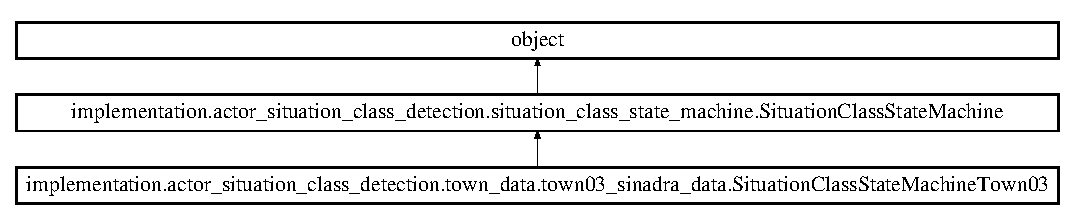
\includegraphics[height=2.503726cm]{classimplementation_1_1actor__situation__class__detection_1_1town__data_1_1town03__sinadra__data51d2866043798c330fb9ba17644a4a6f}
\end{center}
\end{figure}
\doxysubsection*{Public Member Functions}
\begin{DoxyCompactItemize}
\item 
def \mbox{\hyperlink{classimplementation_1_1actor__situation__class__detection_1_1town__data_1_1town03__sinadra__data51d2866043798c330fb9ba17644a4a6f_a247f387d4016f760cb64c3c348db587e}{\+\_\+\+\_\+init\+\_\+\+\_\+}} (self)
\end{DoxyCompactItemize}
\doxysubsection*{Additional Inherited Members}


\doxysubsection{Detailed Description}
\begin{DoxyVerb}This class represents an initialized situation class state machine for CARLA Town03.
\end{DoxyVerb}
 

\doxysubsection{Constructor \& Destructor Documentation}
\mbox{\Hypertarget{classimplementation_1_1actor__situation__class__detection_1_1town__data_1_1town03__sinadra__data51d2866043798c330fb9ba17644a4a6f_a247f387d4016f760cb64c3c348db587e}\label{classimplementation_1_1actor__situation__class__detection_1_1town__data_1_1town03__sinadra__data51d2866043798c330fb9ba17644a4a6f_a247f387d4016f760cb64c3c348db587e}} 
\index{implementation.actor\_situation\_class\_detection.town\_data.town03\_sinadra\_data.SituationClassStateMachineTown03@{implementation.actor\_situation\_class\_detection.town\_data.town03\_sinadra\_data.SituationClassStateMachineTown03}!\_\_init\_\_@{\_\_init\_\_}}
\index{\_\_init\_\_@{\_\_init\_\_}!implementation.actor\_situation\_class\_detection.town\_data.town03\_sinadra\_data.SituationClassStateMachineTown03@{implementation.actor\_situation\_class\_detection.town\_data.town03\_sinadra\_data.SituationClassStateMachineTown03}}
\doxysubsubsection{\texorpdfstring{\_\_init\_\_()}{\_\_init\_\_()}}
{\footnotesize\ttfamily def implementation.\+actor\+\_\+situation\+\_\+class\+\_\+detection.\+town\+\_\+data.\+town03\+\_\+sinadra\+\_\+data.\+Situation\+Class\+State\+Machine\+Town03.\+\_\+\+\_\+init\+\_\+\+\_\+ (\begin{DoxyParamCaption}\item[{}]{self }\end{DoxyParamCaption})}



The documentation for this class was generated from the following file\+:\begin{DoxyCompactItemize}
\item 
implementation/actor\+\_\+situation\+\_\+class\+\_\+detection/town\+\_\+data/\mbox{\hyperlink{town03__sinadra__data_8py}{town03\+\_\+sinadra\+\_\+data.\+py}}\end{DoxyCompactItemize}

\hypertarget{classimplementation_1_1actor__situation__class__detection_1_1situation__class_1_1_situation_class_type}{}\section{implementation.\+actor\+\_\+situation\+\_\+class\+\_\+detection.\+situation\+\_\+class.\+Situation\+Class\+Type Class Reference}
\label{classimplementation_1_1actor__situation__class__detection_1_1situation__class_1_1_situation_class_type}\index{implementation.\+actor\+\_\+situation\+\_\+class\+\_\+detection.\+situation\+\_\+class.\+Situation\+Class\+Type@{implementation.\+actor\+\_\+situation\+\_\+class\+\_\+detection.\+situation\+\_\+class.\+Situation\+Class\+Type}}
Inheritance diagram for implementation.\+actor\+\_\+situation\+\_\+class\+\_\+detection.\+situation\+\_\+class.\+Situation\+Class\+Type\+:\begin{figure}[H]
\begin{center}
\leavevmode
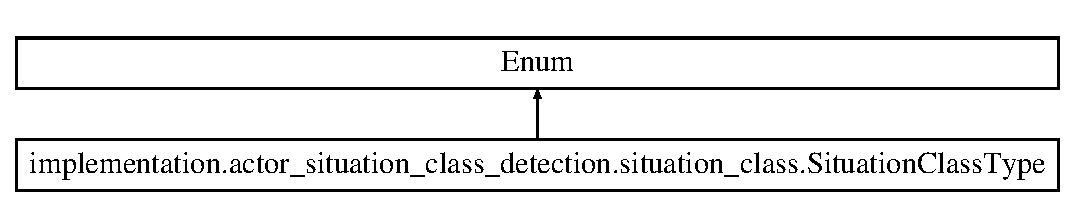
\includegraphics[height=2.000000cm]{classimplementation_1_1actor__situation__class__detection_1_1situation__class_1_1_situation_class_type}
\end{center}
\end{figure}
\subsection*{Static Public Attributes}
\begin{DoxyCompactItemize}
\item 
int \hyperlink{classimplementation_1_1actor__situation__class__detection_1_1situation__class_1_1_situation_class_type_a265c63027258d4b55271cc723cb696a8}{F\+O\+L\+L\+O\+W\+I\+N\+G\+\_\+\+L\+A\+N\+E\+\_\+1\+\_\+\+L\+A\+NE} = 1
\item 
int \hyperlink{classimplementation_1_1actor__situation__class__detection_1_1situation__class_1_1_situation_class_type_a83453d8bbf3d47c3ebb44fc75183aa77}{F\+O\+L\+L\+O\+W\+I\+N\+G\+\_\+\+L\+A\+N\+E\+\_\+2\+\_\+\+L\+A\+N\+ES} = 2
\item 
int \hyperlink{classimplementation_1_1actor__situation__class__detection_1_1situation__class_1_1_situation_class_type_abcfeb3c7fa647038317448846c9834fe}{M\+E\+R\+G\+I\+N\+G\+\_\+\+L\+A\+N\+ES} = 3
\item 
int \hyperlink{classimplementation_1_1actor__situation__class__detection_1_1situation__class_1_1_situation_class_type_a3cf35050d8937317d775473de02ea86e}{S\+I\+G\+N\+A\+L\+I\+Z\+E\+D\+\_\+\+T\+\_\+\+C\+R\+O\+S\+S\+I\+N\+G\+\_\+2\+\_\+\+L\+A\+N\+ES} = 4
\item 
int \hyperlink{classimplementation_1_1actor__situation__class__detection_1_1situation__class_1_1_situation_class_type_a1a8e6e2308d740f6c0e611129d991ee2}{U\+N\+S\+I\+G\+N\+A\+L\+I\+Z\+E\+D\+\_\+\+T\+\_\+\+C\+R\+O\+S\+S\+I\+N\+G\+\_\+2\+\_\+\+L\+A\+N\+ES} = 5
\item 
int \hyperlink{classimplementation_1_1actor__situation__class__detection_1_1situation__class_1_1_situation_class_type_a3a5d96fb10a8d4bd210fccbd808a0167}{S\+I\+G\+N\+A\+L\+I\+Z\+E\+D\+\_\+4\+\_\+\+W\+A\+Y\+\_\+\+C\+R\+O\+S\+S\+I\+NG} = 6
\item 
int \hyperlink{classimplementation_1_1actor__situation__class__detection_1_1situation__class_1_1_situation_class_type_ad826eb0f403ae25454c93f66aca1d750}{U\+N\+S\+I\+G\+N\+A\+L\+I\+Z\+E\+D\+\_\+4\+\_\+\+W\+A\+Y\+\_\+\+C\+R\+O\+S\+S\+I\+NG} = 7
\item 
int \hyperlink{classimplementation_1_1actor__situation__class__detection_1_1situation__class_1_1_situation_class_type_afe96548ef6e393ce55333d68f466c06c}{M\+I\+S\+C\+E\+L\+L\+A\+N\+E\+O\+US} = 8
\end{DoxyCompactItemize}


\subsection{Member Data Documentation}
\mbox{\Hypertarget{classimplementation_1_1actor__situation__class__detection_1_1situation__class_1_1_situation_class_type_a265c63027258d4b55271cc723cb696a8}\label{classimplementation_1_1actor__situation__class__detection_1_1situation__class_1_1_situation_class_type_a265c63027258d4b55271cc723cb696a8}} 
\index{implementation\+::actor\+\_\+situation\+\_\+class\+\_\+detection\+::situation\+\_\+class\+::\+Situation\+Class\+Type@{implementation\+::actor\+\_\+situation\+\_\+class\+\_\+detection\+::situation\+\_\+class\+::\+Situation\+Class\+Type}!F\+O\+L\+L\+O\+W\+I\+N\+G\+\_\+\+L\+A\+N\+E\+\_\+1\+\_\+\+L\+A\+NE@{F\+O\+L\+L\+O\+W\+I\+N\+G\+\_\+\+L\+A\+N\+E\+\_\+1\+\_\+\+L\+A\+NE}}
\index{F\+O\+L\+L\+O\+W\+I\+N\+G\+\_\+\+L\+A\+N\+E\+\_\+1\+\_\+\+L\+A\+NE@{F\+O\+L\+L\+O\+W\+I\+N\+G\+\_\+\+L\+A\+N\+E\+\_\+1\+\_\+\+L\+A\+NE}!implementation\+::actor\+\_\+situation\+\_\+class\+\_\+detection\+::situation\+\_\+class\+::\+Situation\+Class\+Type@{implementation\+::actor\+\_\+situation\+\_\+class\+\_\+detection\+::situation\+\_\+class\+::\+Situation\+Class\+Type}}
\subsubsection{\texorpdfstring{F\+O\+L\+L\+O\+W\+I\+N\+G\+\_\+\+L\+A\+N\+E\+\_\+1\+\_\+\+L\+A\+NE}{FOLLOWING\_LANE\_1\_LANE}}
{\footnotesize\ttfamily int implementation.\+actor\+\_\+situation\+\_\+class\+\_\+detection.\+situation\+\_\+class.\+Situation\+Class\+Type.\+F\+O\+L\+L\+O\+W\+I\+N\+G\+\_\+\+L\+A\+N\+E\+\_\+1\+\_\+\+L\+A\+NE = 1\hspace{0.3cm}{\ttfamily [static]}}

\mbox{\Hypertarget{classimplementation_1_1actor__situation__class__detection_1_1situation__class_1_1_situation_class_type_a83453d8bbf3d47c3ebb44fc75183aa77}\label{classimplementation_1_1actor__situation__class__detection_1_1situation__class_1_1_situation_class_type_a83453d8bbf3d47c3ebb44fc75183aa77}} 
\index{implementation\+::actor\+\_\+situation\+\_\+class\+\_\+detection\+::situation\+\_\+class\+::\+Situation\+Class\+Type@{implementation\+::actor\+\_\+situation\+\_\+class\+\_\+detection\+::situation\+\_\+class\+::\+Situation\+Class\+Type}!F\+O\+L\+L\+O\+W\+I\+N\+G\+\_\+\+L\+A\+N\+E\+\_\+2\+\_\+\+L\+A\+N\+ES@{F\+O\+L\+L\+O\+W\+I\+N\+G\+\_\+\+L\+A\+N\+E\+\_\+2\+\_\+\+L\+A\+N\+ES}}
\index{F\+O\+L\+L\+O\+W\+I\+N\+G\+\_\+\+L\+A\+N\+E\+\_\+2\+\_\+\+L\+A\+N\+ES@{F\+O\+L\+L\+O\+W\+I\+N\+G\+\_\+\+L\+A\+N\+E\+\_\+2\+\_\+\+L\+A\+N\+ES}!implementation\+::actor\+\_\+situation\+\_\+class\+\_\+detection\+::situation\+\_\+class\+::\+Situation\+Class\+Type@{implementation\+::actor\+\_\+situation\+\_\+class\+\_\+detection\+::situation\+\_\+class\+::\+Situation\+Class\+Type}}
\subsubsection{\texorpdfstring{F\+O\+L\+L\+O\+W\+I\+N\+G\+\_\+\+L\+A\+N\+E\+\_\+2\+\_\+\+L\+A\+N\+ES}{FOLLOWING\_LANE\_2\_LANES}}
{\footnotesize\ttfamily int implementation.\+actor\+\_\+situation\+\_\+class\+\_\+detection.\+situation\+\_\+class.\+Situation\+Class\+Type.\+F\+O\+L\+L\+O\+W\+I\+N\+G\+\_\+\+L\+A\+N\+E\+\_\+2\+\_\+\+L\+A\+N\+ES = 2\hspace{0.3cm}{\ttfamily [static]}}

\mbox{\Hypertarget{classimplementation_1_1actor__situation__class__detection_1_1situation__class_1_1_situation_class_type_abcfeb3c7fa647038317448846c9834fe}\label{classimplementation_1_1actor__situation__class__detection_1_1situation__class_1_1_situation_class_type_abcfeb3c7fa647038317448846c9834fe}} 
\index{implementation\+::actor\+\_\+situation\+\_\+class\+\_\+detection\+::situation\+\_\+class\+::\+Situation\+Class\+Type@{implementation\+::actor\+\_\+situation\+\_\+class\+\_\+detection\+::situation\+\_\+class\+::\+Situation\+Class\+Type}!M\+E\+R\+G\+I\+N\+G\+\_\+\+L\+A\+N\+ES@{M\+E\+R\+G\+I\+N\+G\+\_\+\+L\+A\+N\+ES}}
\index{M\+E\+R\+G\+I\+N\+G\+\_\+\+L\+A\+N\+ES@{M\+E\+R\+G\+I\+N\+G\+\_\+\+L\+A\+N\+ES}!implementation\+::actor\+\_\+situation\+\_\+class\+\_\+detection\+::situation\+\_\+class\+::\+Situation\+Class\+Type@{implementation\+::actor\+\_\+situation\+\_\+class\+\_\+detection\+::situation\+\_\+class\+::\+Situation\+Class\+Type}}
\subsubsection{\texorpdfstring{M\+E\+R\+G\+I\+N\+G\+\_\+\+L\+A\+N\+ES}{MERGING\_LANES}}
{\footnotesize\ttfamily int implementation.\+actor\+\_\+situation\+\_\+class\+\_\+detection.\+situation\+\_\+class.\+Situation\+Class\+Type.\+M\+E\+R\+G\+I\+N\+G\+\_\+\+L\+A\+N\+ES = 3\hspace{0.3cm}{\ttfamily [static]}}

\mbox{\Hypertarget{classimplementation_1_1actor__situation__class__detection_1_1situation__class_1_1_situation_class_type_afe96548ef6e393ce55333d68f466c06c}\label{classimplementation_1_1actor__situation__class__detection_1_1situation__class_1_1_situation_class_type_afe96548ef6e393ce55333d68f466c06c}} 
\index{implementation\+::actor\+\_\+situation\+\_\+class\+\_\+detection\+::situation\+\_\+class\+::\+Situation\+Class\+Type@{implementation\+::actor\+\_\+situation\+\_\+class\+\_\+detection\+::situation\+\_\+class\+::\+Situation\+Class\+Type}!M\+I\+S\+C\+E\+L\+L\+A\+N\+E\+O\+US@{M\+I\+S\+C\+E\+L\+L\+A\+N\+E\+O\+US}}
\index{M\+I\+S\+C\+E\+L\+L\+A\+N\+E\+O\+US@{M\+I\+S\+C\+E\+L\+L\+A\+N\+E\+O\+US}!implementation\+::actor\+\_\+situation\+\_\+class\+\_\+detection\+::situation\+\_\+class\+::\+Situation\+Class\+Type@{implementation\+::actor\+\_\+situation\+\_\+class\+\_\+detection\+::situation\+\_\+class\+::\+Situation\+Class\+Type}}
\subsubsection{\texorpdfstring{M\+I\+S\+C\+E\+L\+L\+A\+N\+E\+O\+US}{MISCELLANEOUS}}
{\footnotesize\ttfamily int implementation.\+actor\+\_\+situation\+\_\+class\+\_\+detection.\+situation\+\_\+class.\+Situation\+Class\+Type.\+M\+I\+S\+C\+E\+L\+L\+A\+N\+E\+O\+US = 8\hspace{0.3cm}{\ttfamily [static]}}

\mbox{\Hypertarget{classimplementation_1_1actor__situation__class__detection_1_1situation__class_1_1_situation_class_type_a3a5d96fb10a8d4bd210fccbd808a0167}\label{classimplementation_1_1actor__situation__class__detection_1_1situation__class_1_1_situation_class_type_a3a5d96fb10a8d4bd210fccbd808a0167}} 
\index{implementation\+::actor\+\_\+situation\+\_\+class\+\_\+detection\+::situation\+\_\+class\+::\+Situation\+Class\+Type@{implementation\+::actor\+\_\+situation\+\_\+class\+\_\+detection\+::situation\+\_\+class\+::\+Situation\+Class\+Type}!S\+I\+G\+N\+A\+L\+I\+Z\+E\+D\+\_\+4\+\_\+\+W\+A\+Y\+\_\+\+C\+R\+O\+S\+S\+I\+NG@{S\+I\+G\+N\+A\+L\+I\+Z\+E\+D\+\_\+4\+\_\+\+W\+A\+Y\+\_\+\+C\+R\+O\+S\+S\+I\+NG}}
\index{S\+I\+G\+N\+A\+L\+I\+Z\+E\+D\+\_\+4\+\_\+\+W\+A\+Y\+\_\+\+C\+R\+O\+S\+S\+I\+NG@{S\+I\+G\+N\+A\+L\+I\+Z\+E\+D\+\_\+4\+\_\+\+W\+A\+Y\+\_\+\+C\+R\+O\+S\+S\+I\+NG}!implementation\+::actor\+\_\+situation\+\_\+class\+\_\+detection\+::situation\+\_\+class\+::\+Situation\+Class\+Type@{implementation\+::actor\+\_\+situation\+\_\+class\+\_\+detection\+::situation\+\_\+class\+::\+Situation\+Class\+Type}}
\subsubsection{\texorpdfstring{S\+I\+G\+N\+A\+L\+I\+Z\+E\+D\+\_\+4\+\_\+\+W\+A\+Y\+\_\+\+C\+R\+O\+S\+S\+I\+NG}{SIGNALIZED\_4\_WAY\_CROSSING}}
{\footnotesize\ttfamily int implementation.\+actor\+\_\+situation\+\_\+class\+\_\+detection.\+situation\+\_\+class.\+Situation\+Class\+Type.\+S\+I\+G\+N\+A\+L\+I\+Z\+E\+D\+\_\+4\+\_\+\+W\+A\+Y\+\_\+\+C\+R\+O\+S\+S\+I\+NG = 6\hspace{0.3cm}{\ttfamily [static]}}

\mbox{\Hypertarget{classimplementation_1_1actor__situation__class__detection_1_1situation__class_1_1_situation_class_type_a3cf35050d8937317d775473de02ea86e}\label{classimplementation_1_1actor__situation__class__detection_1_1situation__class_1_1_situation_class_type_a3cf35050d8937317d775473de02ea86e}} 
\index{implementation\+::actor\+\_\+situation\+\_\+class\+\_\+detection\+::situation\+\_\+class\+::\+Situation\+Class\+Type@{implementation\+::actor\+\_\+situation\+\_\+class\+\_\+detection\+::situation\+\_\+class\+::\+Situation\+Class\+Type}!S\+I\+G\+N\+A\+L\+I\+Z\+E\+D\+\_\+\+T\+\_\+\+C\+R\+O\+S\+S\+I\+N\+G\+\_\+2\+\_\+\+L\+A\+N\+ES@{S\+I\+G\+N\+A\+L\+I\+Z\+E\+D\+\_\+\+T\+\_\+\+C\+R\+O\+S\+S\+I\+N\+G\+\_\+2\+\_\+\+L\+A\+N\+ES}}
\index{S\+I\+G\+N\+A\+L\+I\+Z\+E\+D\+\_\+\+T\+\_\+\+C\+R\+O\+S\+S\+I\+N\+G\+\_\+2\+\_\+\+L\+A\+N\+ES@{S\+I\+G\+N\+A\+L\+I\+Z\+E\+D\+\_\+\+T\+\_\+\+C\+R\+O\+S\+S\+I\+N\+G\+\_\+2\+\_\+\+L\+A\+N\+ES}!implementation\+::actor\+\_\+situation\+\_\+class\+\_\+detection\+::situation\+\_\+class\+::\+Situation\+Class\+Type@{implementation\+::actor\+\_\+situation\+\_\+class\+\_\+detection\+::situation\+\_\+class\+::\+Situation\+Class\+Type}}
\subsubsection{\texorpdfstring{S\+I\+G\+N\+A\+L\+I\+Z\+E\+D\+\_\+\+T\+\_\+\+C\+R\+O\+S\+S\+I\+N\+G\+\_\+2\+\_\+\+L\+A\+N\+ES}{SIGNALIZED\_T\_CROSSING\_2\_LANES}}
{\footnotesize\ttfamily int implementation.\+actor\+\_\+situation\+\_\+class\+\_\+detection.\+situation\+\_\+class.\+Situation\+Class\+Type.\+S\+I\+G\+N\+A\+L\+I\+Z\+E\+D\+\_\+\+T\+\_\+\+C\+R\+O\+S\+S\+I\+N\+G\+\_\+2\+\_\+\+L\+A\+N\+ES = 4\hspace{0.3cm}{\ttfamily [static]}}

\mbox{\Hypertarget{classimplementation_1_1actor__situation__class__detection_1_1situation__class_1_1_situation_class_type_ad826eb0f403ae25454c93f66aca1d750}\label{classimplementation_1_1actor__situation__class__detection_1_1situation__class_1_1_situation_class_type_ad826eb0f403ae25454c93f66aca1d750}} 
\index{implementation\+::actor\+\_\+situation\+\_\+class\+\_\+detection\+::situation\+\_\+class\+::\+Situation\+Class\+Type@{implementation\+::actor\+\_\+situation\+\_\+class\+\_\+detection\+::situation\+\_\+class\+::\+Situation\+Class\+Type}!U\+N\+S\+I\+G\+N\+A\+L\+I\+Z\+E\+D\+\_\+4\+\_\+\+W\+A\+Y\+\_\+\+C\+R\+O\+S\+S\+I\+NG@{U\+N\+S\+I\+G\+N\+A\+L\+I\+Z\+E\+D\+\_\+4\+\_\+\+W\+A\+Y\+\_\+\+C\+R\+O\+S\+S\+I\+NG}}
\index{U\+N\+S\+I\+G\+N\+A\+L\+I\+Z\+E\+D\+\_\+4\+\_\+\+W\+A\+Y\+\_\+\+C\+R\+O\+S\+S\+I\+NG@{U\+N\+S\+I\+G\+N\+A\+L\+I\+Z\+E\+D\+\_\+4\+\_\+\+W\+A\+Y\+\_\+\+C\+R\+O\+S\+S\+I\+NG}!implementation\+::actor\+\_\+situation\+\_\+class\+\_\+detection\+::situation\+\_\+class\+::\+Situation\+Class\+Type@{implementation\+::actor\+\_\+situation\+\_\+class\+\_\+detection\+::situation\+\_\+class\+::\+Situation\+Class\+Type}}
\subsubsection{\texorpdfstring{U\+N\+S\+I\+G\+N\+A\+L\+I\+Z\+E\+D\+\_\+4\+\_\+\+W\+A\+Y\+\_\+\+C\+R\+O\+S\+S\+I\+NG}{UNSIGNALIZED\_4\_WAY\_CROSSING}}
{\footnotesize\ttfamily int implementation.\+actor\+\_\+situation\+\_\+class\+\_\+detection.\+situation\+\_\+class.\+Situation\+Class\+Type.\+U\+N\+S\+I\+G\+N\+A\+L\+I\+Z\+E\+D\+\_\+4\+\_\+\+W\+A\+Y\+\_\+\+C\+R\+O\+S\+S\+I\+NG = 7\hspace{0.3cm}{\ttfamily [static]}}

\mbox{\Hypertarget{classimplementation_1_1actor__situation__class__detection_1_1situation__class_1_1_situation_class_type_a1a8e6e2308d740f6c0e611129d991ee2}\label{classimplementation_1_1actor__situation__class__detection_1_1situation__class_1_1_situation_class_type_a1a8e6e2308d740f6c0e611129d991ee2}} 
\index{implementation\+::actor\+\_\+situation\+\_\+class\+\_\+detection\+::situation\+\_\+class\+::\+Situation\+Class\+Type@{implementation\+::actor\+\_\+situation\+\_\+class\+\_\+detection\+::situation\+\_\+class\+::\+Situation\+Class\+Type}!U\+N\+S\+I\+G\+N\+A\+L\+I\+Z\+E\+D\+\_\+\+T\+\_\+\+C\+R\+O\+S\+S\+I\+N\+G\+\_\+2\+\_\+\+L\+A\+N\+ES@{U\+N\+S\+I\+G\+N\+A\+L\+I\+Z\+E\+D\+\_\+\+T\+\_\+\+C\+R\+O\+S\+S\+I\+N\+G\+\_\+2\+\_\+\+L\+A\+N\+ES}}
\index{U\+N\+S\+I\+G\+N\+A\+L\+I\+Z\+E\+D\+\_\+\+T\+\_\+\+C\+R\+O\+S\+S\+I\+N\+G\+\_\+2\+\_\+\+L\+A\+N\+ES@{U\+N\+S\+I\+G\+N\+A\+L\+I\+Z\+E\+D\+\_\+\+T\+\_\+\+C\+R\+O\+S\+S\+I\+N\+G\+\_\+2\+\_\+\+L\+A\+N\+ES}!implementation\+::actor\+\_\+situation\+\_\+class\+\_\+detection\+::situation\+\_\+class\+::\+Situation\+Class\+Type@{implementation\+::actor\+\_\+situation\+\_\+class\+\_\+detection\+::situation\+\_\+class\+::\+Situation\+Class\+Type}}
\subsubsection{\texorpdfstring{U\+N\+S\+I\+G\+N\+A\+L\+I\+Z\+E\+D\+\_\+\+T\+\_\+\+C\+R\+O\+S\+S\+I\+N\+G\+\_\+2\+\_\+\+L\+A\+N\+ES}{UNSIGNALIZED\_T\_CROSSING\_2\_LANES}}
{\footnotesize\ttfamily int implementation.\+actor\+\_\+situation\+\_\+class\+\_\+detection.\+situation\+\_\+class.\+Situation\+Class\+Type.\+U\+N\+S\+I\+G\+N\+A\+L\+I\+Z\+E\+D\+\_\+\+T\+\_\+\+C\+R\+O\+S\+S\+I\+N\+G\+\_\+2\+\_\+\+L\+A\+N\+ES = 5\hspace{0.3cm}{\ttfamily [static]}}



The documentation for this class was generated from the following file\+:\begin{DoxyCompactItemize}
\item 
implementation/actor\+\_\+situation\+\_\+class\+\_\+detection/\hyperlink{situation__class_8py}{situation\+\_\+class.\+py}\end{DoxyCompactItemize}

\hypertarget{classimplementation_1_1data__model_1_1environment_1_1_sun}{}\section{implementation.\+data\+\_\+model.\+environment.\+Sun Class Reference}
\label{classimplementation_1_1data__model_1_1environment_1_1_sun}\index{implementation.\+data\+\_\+model.\+environment.\+Sun@{implementation.\+data\+\_\+model.\+environment.\+Sun}}
\subsection*{Static Public Attributes}
\begin{DoxyCompactItemize}
\item 
\hyperlink{classimplementation_1_1data__model_1_1environment_1_1_sun_ae4abaa94c84d5a3a3b3804f4a5da9601}{float}
\end{DoxyCompactItemize}


\subsection{Member Data Documentation}
\mbox{\Hypertarget{classimplementation_1_1data__model_1_1environment_1_1_sun_ae4abaa94c84d5a3a3b3804f4a5da9601}\label{classimplementation_1_1data__model_1_1environment_1_1_sun_ae4abaa94c84d5a3a3b3804f4a5da9601}} 
\index{implementation\+::data\+\_\+model\+::environment\+::\+Sun@{implementation\+::data\+\_\+model\+::environment\+::\+Sun}!float@{float}}
\index{float@{float}!implementation\+::data\+\_\+model\+::environment\+::\+Sun@{implementation\+::data\+\_\+model\+::environment\+::\+Sun}}
\subsubsection{\texorpdfstring{float}{float}}
{\footnotesize\ttfamily implementation.\+data\+\_\+model.\+environment.\+Sun.\+float\hspace{0.3cm}{\ttfamily [static]}}



The documentation for this class was generated from the following file\+:\begin{DoxyCompactItemize}
\item 
implementation/data\+\_\+model/\hyperlink{environment_8py}{environment.\+py}\end{DoxyCompactItemize}

\hypertarget{classimplementation_1_1data__model_1_1vehicle_1_1_surrounding_vehicles}{}\section{implementation.\+data\+\_\+model.\+vehicle.\+Surrounding\+Vehicles Class Reference}
\label{classimplementation_1_1data__model_1_1vehicle_1_1_surrounding_vehicles}\index{implementation.\+data\+\_\+model.\+vehicle.\+Surrounding\+Vehicles@{implementation.\+data\+\_\+model.\+vehicle.\+Surrounding\+Vehicles}}


The documentation for this class was generated from the following file\+:\begin{DoxyCompactItemize}
\item 
implementation/data\+\_\+model/\hyperlink{vehicle_8py}{vehicle.\+py}\end{DoxyCompactItemize}

\hypertarget{classimplementation_1_1data__model_1_1environment_1_1_time_of_day}{}\section{implementation.\+data\+\_\+model.\+environment.\+Time\+Of\+Day Class Reference}
\label{classimplementation_1_1data__model_1_1environment_1_1_time_of_day}\index{implementation.\+data\+\_\+model.\+environment.\+Time\+Of\+Day@{implementation.\+data\+\_\+model.\+environment.\+Time\+Of\+Day}}
\subsection*{Static Public Attributes}
\begin{DoxyCompactItemize}
\item 
\hyperlink{classimplementation_1_1data__model_1_1environment_1_1_time_of_day_a674b9c8933e6386ccb97c676a2c498b0}{bool}
\end{DoxyCompactItemize}


\subsection{Member Data Documentation}
\mbox{\Hypertarget{classimplementation_1_1data__model_1_1environment_1_1_time_of_day_a674b9c8933e6386ccb97c676a2c498b0}\label{classimplementation_1_1data__model_1_1environment_1_1_time_of_day_a674b9c8933e6386ccb97c676a2c498b0}} 
\index{implementation\+::data\+\_\+model\+::environment\+::\+Time\+Of\+Day@{implementation\+::data\+\_\+model\+::environment\+::\+Time\+Of\+Day}!bool@{bool}}
\index{bool@{bool}!implementation\+::data\+\_\+model\+::environment\+::\+Time\+Of\+Day@{implementation\+::data\+\_\+model\+::environment\+::\+Time\+Of\+Day}}
\subsubsection{\texorpdfstring{bool}{bool}}
{\footnotesize\ttfamily implementation.\+data\+\_\+model.\+environment.\+Time\+Of\+Day.\+bool\hspace{0.3cm}{\ttfamily [static]}}



The documentation for this class was generated from the following file\+:\begin{DoxyCompactItemize}
\item 
implementation/data\+\_\+model/\hyperlink{environment_8py}{environment.\+py}\end{DoxyCompactItemize}

\hypertarget{classimplementation_1_1data__model_1_1positions_1_1_trajectory_position}{}\section{implementation.\+data\+\_\+model.\+positions.\+Trajectory\+Position Class Reference}
\label{classimplementation_1_1data__model_1_1positions_1_1_trajectory_position}\index{implementation.\+data\+\_\+model.\+positions.\+Trajectory\+Position@{implementation.\+data\+\_\+model.\+positions.\+Trajectory\+Position}}
\subsection*{Static Public Attributes}
\begin{DoxyCompactItemize}
\item 
\hyperlink{classimplementation_1_1data__model_1_1positions_1_1_trajectory_position_a041cb25c7a664bf191fb5352eb17777e}{Orientation}
\item 
\hyperlink{classimplementation_1_1data__model_1_1positions_1_1_trajectory_position_a44fdd4af154797d918be465ee73f3765}{float}
\end{DoxyCompactItemize}


\subsection{Member Data Documentation}
\mbox{\Hypertarget{classimplementation_1_1data__model_1_1positions_1_1_trajectory_position_a44fdd4af154797d918be465ee73f3765}\label{classimplementation_1_1data__model_1_1positions_1_1_trajectory_position_a44fdd4af154797d918be465ee73f3765}} 
\index{implementation\+::data\+\_\+model\+::positions\+::\+Trajectory\+Position@{implementation\+::data\+\_\+model\+::positions\+::\+Trajectory\+Position}!float@{float}}
\index{float@{float}!implementation\+::data\+\_\+model\+::positions\+::\+Trajectory\+Position@{implementation\+::data\+\_\+model\+::positions\+::\+Trajectory\+Position}}
\subsubsection{\texorpdfstring{float}{float}}
{\footnotesize\ttfamily implementation.\+data\+\_\+model.\+positions.\+Trajectory\+Position.\+float\hspace{0.3cm}{\ttfamily [static]}}

\mbox{\Hypertarget{classimplementation_1_1data__model_1_1positions_1_1_trajectory_position_a041cb25c7a664bf191fb5352eb17777e}\label{classimplementation_1_1data__model_1_1positions_1_1_trajectory_position_a041cb25c7a664bf191fb5352eb17777e}} 
\index{implementation\+::data\+\_\+model\+::positions\+::\+Trajectory\+Position@{implementation\+::data\+\_\+model\+::positions\+::\+Trajectory\+Position}!Orientation@{Orientation}}
\index{Orientation@{Orientation}!implementation\+::data\+\_\+model\+::positions\+::\+Trajectory\+Position@{implementation\+::data\+\_\+model\+::positions\+::\+Trajectory\+Position}}
\subsubsection{\texorpdfstring{Orientation}{Orientation}}
{\footnotesize\ttfamily implementation.\+data\+\_\+model.\+positions.\+Trajectory\+Position.\+Orientation\hspace{0.3cm}{\ttfamily [static]}}



The documentation for this class was generated from the following file\+:\begin{DoxyCompactItemize}
\item 
implementation/data\+\_\+model/\hyperlink{positions_8py}{positions.\+py}\end{DoxyCompactItemize}

\hypertarget{classimplementation_1_1actor__situation__class__detection_1_1bayesian__network__id__selection_1_ad1cbe3342f1a4b96bc86989d1def5fb}{}\doxysection{implementation.\+actor\+\_\+situation\+\_\+class\+\_\+detection.\+bayesian\+\_\+network\+\_\+id\+\_\+selection.\+two\+\_\+lane\+\_\+following\+\_\+bn\+\_\+id\+\_\+selector.\+Two\+Lane\+Following\+B\+N\+Id\+Selector Class Reference}
\label{classimplementation_1_1actor__situation__class__detection_1_1bayesian__network__id__selection_1_ad1cbe3342f1a4b96bc86989d1def5fb}\index{implementation.actor\_situation\_class\_detection.bayesian\_network\_id\_selection.two\_lane\_following\_bn\_id\_selector.TwoLaneFollowingBNIdSelector@{implementation.actor\_situation\_class\_detection.bayesian\_network\_id\_selection.two\_lane\_following\_bn\_id\_selector.TwoLaneFollowingBNIdSelector}}
Inheritance diagram for implementation.\+actor\+\_\+situation\+\_\+class\+\_\+detection.\+bayesian\+\_\+network\+\_\+id\+\_\+selection.\+two\+\_\+lane\+\_\+following\+\_\+bn\+\_\+id\+\_\+selector.\+Two\+Lane\+Following\+B\+N\+Id\+Selector\+:\begin{figure}[H]
\begin{center}
\leavevmode
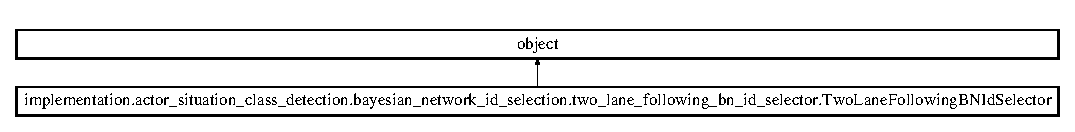
\includegraphics[height=1.323877cm]{classimplementation_1_1actor__situation__class__detection_1_1bayesian__network__id__selection_1_ad1cbe3342f1a4b96bc86989d1def5fb}
\end{center}
\end{figure}
\doxysubsection*{Public Member Functions}
\begin{DoxyCompactItemize}
\item 
def \mbox{\hyperlink{classimplementation_1_1actor__situation__class__detection_1_1bayesian__network__id__selection_1_ad1cbe3342f1a4b96bc86989d1def5fb_af48d70e11be3d8f9b064f28416805cf0}{\+\_\+\+\_\+init\+\_\+\+\_\+}} (self, \mbox{\hyperlink{classimplementation_1_1actor__situation__class__detection_1_1situation__class_1_1_two_lane_following_situation_class}{Two\+Lane\+Following\+Situation\+Class}} hero\+\_\+situation\+\_\+class, \mbox{\hyperlink{classimplementation_1_1actor__situation__class__detection_1_1vehicle__actor__wrapper_1_1_vehicle_actor_wrapper}{Vehicle\+Actor\+Wrapper}} wrapped\+\_\+hero\+\_\+vehicle, List\mbox{[}\char`\"{}Vehicle\+Actor\+Wrapper\char`\"{}\mbox{]} wrapped\+\_\+other\+\_\+vehicles, carla.\+Map carla\+\_\+map, carla.\+Debug\+Helper carla\+\_\+debug\+\_\+helper)
\item 
List\mbox{[}\char`\"{}Vehicle\+Dependent\+B\+N\+Id\char`\"{}\mbox{]} \mbox{\hyperlink{classimplementation_1_1actor__situation__class__detection_1_1bayesian__network__id__selection_1_ad1cbe3342f1a4b96bc86989d1def5fb_af516b932d8c563794d803b70908a8ce2}{get\+\_\+vehicle\+\_\+dependent\+\_\+bn\+\_\+ids\+\_\+for\+\_\+two\+\_\+lane\+\_\+following\+\_\+sit\+\_\+class}} (self)
\end{DoxyCompactItemize}


\doxysubsection{Constructor \& Destructor Documentation}
\mbox{\Hypertarget{classimplementation_1_1actor__situation__class__detection_1_1bayesian__network__id__selection_1_ad1cbe3342f1a4b96bc86989d1def5fb_af48d70e11be3d8f9b064f28416805cf0}\label{classimplementation_1_1actor__situation__class__detection_1_1bayesian__network__id__selection_1_ad1cbe3342f1a4b96bc86989d1def5fb_af48d70e11be3d8f9b064f28416805cf0}} 
\index{implementation.actor\_situation\_class\_detection.bayesian\_network\_id\_selection.two\_lane\_following\_bn\_id\_selector.TwoLaneFollowingBNIdSelector@{implementation.actor\_situation\_class\_detection.bayesian\_network\_id\_selection.two\_lane\_following\_bn\_id\_selector.TwoLaneFollowingBNIdSelector}!\_\_init\_\_@{\_\_init\_\_}}
\index{\_\_init\_\_@{\_\_init\_\_}!implementation.actor\_situation\_class\_detection.bayesian\_network\_id\_selection.two\_lane\_following\_bn\_id\_selector.TwoLaneFollowingBNIdSelector@{implementation.actor\_situation\_class\_detection.bayesian\_network\_id\_selection.two\_lane\_following\_bn\_id\_selector.TwoLaneFollowingBNIdSelector}}
\doxysubsubsection{\texorpdfstring{\_\_init\_\_()}{\_\_init\_\_()}}
{\footnotesize\ttfamily def implementation.\+actor\+\_\+situation\+\_\+class\+\_\+detection.\+bayesian\+\_\+network\+\_\+id\+\_\+selection.\+two\+\_\+lane\+\_\+following\+\_\+bn\+\_\+id\+\_\+selector.\+Two\+Lane\+Following\+B\+N\+Id\+Selector.\+\_\+\+\_\+init\+\_\+\+\_\+ (\begin{DoxyParamCaption}\item[{}]{self,  }\item[{\mbox{\hyperlink{classimplementation_1_1actor__situation__class__detection_1_1situation__class_1_1_two_lane_following_situation_class}{Two\+Lane\+Following\+Situation\+Class}}}]{hero\+\_\+situation\+\_\+class,  }\item[{\mbox{\hyperlink{classimplementation_1_1actor__situation__class__detection_1_1vehicle__actor__wrapper_1_1_vehicle_actor_wrapper}{Vehicle\+Actor\+Wrapper}}}]{wrapped\+\_\+hero\+\_\+vehicle,  }\item[{List\mbox{[}\char`\"{}Vehicle\+Actor\+Wrapper\char`\"{}\mbox{]}}]{wrapped\+\_\+other\+\_\+vehicles,  }\item[{carla.\+Map}]{carla\+\_\+map,  }\item[{carla.\+Debug\+Helper}]{carla\+\_\+debug\+\_\+helper }\end{DoxyParamCaption})}



\doxysubsection{Member Function Documentation}
\mbox{\Hypertarget{classimplementation_1_1actor__situation__class__detection_1_1bayesian__network__id__selection_1_ad1cbe3342f1a4b96bc86989d1def5fb_af516b932d8c563794d803b70908a8ce2}\label{classimplementation_1_1actor__situation__class__detection_1_1bayesian__network__id__selection_1_ad1cbe3342f1a4b96bc86989d1def5fb_af516b932d8c563794d803b70908a8ce2}} 
\index{implementation.actor\_situation\_class\_detection.bayesian\_network\_id\_selection.two\_lane\_following\_bn\_id\_selector.TwoLaneFollowingBNIdSelector@{implementation.actor\_situation\_class\_detection.bayesian\_network\_id\_selection.two\_lane\_following\_bn\_id\_selector.TwoLaneFollowingBNIdSelector}!get\_vehicle\_dependent\_bn\_ids\_for\_two\_lane\_following\_sit\_class@{get\_vehicle\_dependent\_bn\_ids\_for\_two\_lane\_following\_sit\_class}}
\index{get\_vehicle\_dependent\_bn\_ids\_for\_two\_lane\_following\_sit\_class@{get\_vehicle\_dependent\_bn\_ids\_for\_two\_lane\_following\_sit\_class}!implementation.actor\_situation\_class\_detection.bayesian\_network\_id\_selection.two\_lane\_following\_bn\_id\_selector.TwoLaneFollowingBNIdSelector@{implementation.actor\_situation\_class\_detection.bayesian\_network\_id\_selection.two\_lane\_following\_bn\_id\_selector.TwoLaneFollowingBNIdSelector}}
\doxysubsubsection{\texorpdfstring{get\_vehicle\_dependent\_bn\_ids\_for\_two\_lane\_following\_sit\_class()}{get\_vehicle\_dependent\_bn\_ids\_for\_two\_lane\_following\_sit\_class()}}
{\footnotesize\ttfamily  List\mbox{[}\char`\"{}Vehicle\+Dependent\+B\+N\+Id\char`\"{}\mbox{]} implementation.\+actor\+\_\+situation\+\_\+class\+\_\+detection.\+bayesian\+\_\+network\+\_\+id\+\_\+selection.\+two\+\_\+lane\+\_\+following\+\_\+bn\+\_\+id\+\_\+selector.\+Two\+Lane\+Following\+B\+N\+Id\+Selector.\+get\+\_\+vehicle\+\_\+dependent\+\_\+bn\+\_\+ids\+\_\+for\+\_\+two\+\_\+lane\+\_\+following\+\_\+sit\+\_\+class (\begin{DoxyParamCaption}\item[{}]{self }\end{DoxyParamCaption})}

\begin{DoxyVerb}This method determines the bn ids for each vehicle within the sensing areas of the hero vehicle.
Returns a list of VehicleDependentBNId objects, which map the bn ids to the vehicles respectively.

Returns
-------
List[VehicleDependentBNId]
    List of VehicleDependentBNId objects that maps a BN id to a vehicle.
\end{DoxyVerb}
 

The documentation for this class was generated from the following file\+:\begin{DoxyCompactItemize}
\item 
implementation/actor\+\_\+situation\+\_\+class\+\_\+detection/bayesian\+\_\+network\+\_\+id\+\_\+selection/\mbox{\hyperlink{two__lane__following__bn__id__selector_8py}{two\+\_\+lane\+\_\+following\+\_\+bn\+\_\+id\+\_\+selector.\+py}}\end{DoxyCompactItemize}

\hypertarget{classimplementation_1_1actor__situation__class__detection_1_1situation__class_1_1_two_lane_following_situation_class}{}\doxysection{implementation.\+actor\+\_\+situation\+\_\+class\+\_\+detection.\+situation\+\_\+class.\+Two\+Lane\+Following\+Situation\+Class Class Reference}
\label{classimplementation_1_1actor__situation__class__detection_1_1situation__class_1_1_two_lane_following_situation_class}\index{implementation.actor\_situation\_class\_detection.situation\_class.TwoLaneFollowingSituationClass@{implementation.actor\_situation\_class\_detection.situation\_class.TwoLaneFollowingSituationClass}}
Inheritance diagram for implementation.\+actor\+\_\+situation\+\_\+class\+\_\+detection.\+situation\+\_\+class.\+Two\+Lane\+Following\+Situation\+Class\+:\begin{figure}[H]
\begin{center}
\leavevmode
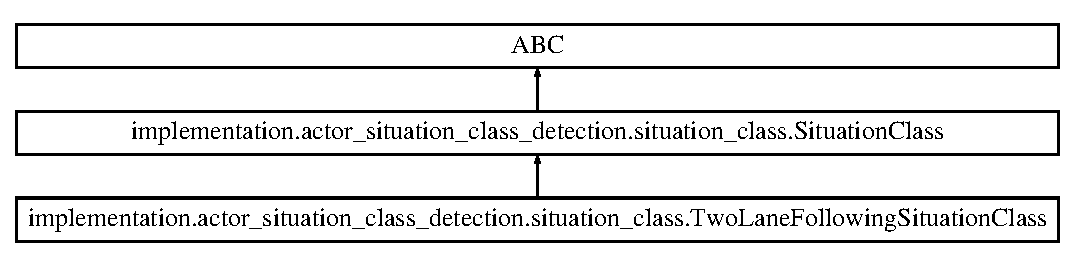
\includegraphics[height=3.000000cm]{classimplementation_1_1actor__situation__class__detection_1_1situation__class_1_1_two_lane_following_situation_class}
\end{center}
\end{figure}
\doxysubsection*{Public Member Functions}
\begin{DoxyCompactItemize}
\item 
def \mbox{\hyperlink{classimplementation_1_1actor__situation__class__detection_1_1situation__class_1_1_two_lane_following_situation_class_a1d100c5367001e45b3b9fbe6c7521149}{\+\_\+\+\_\+init\+\_\+\+\_\+}} (self, str \mbox{\hyperlink{classimplementation_1_1actor__situation__class__detection_1_1situation__class_1_1_situation_class_a27d4d3259b8bb96107692e2b936ce801}{id}}, List\mbox{[}float\mbox{]} situation\+\_\+class\+\_\+polygon\+\_\+coordinates, List\mbox{[}float\mbox{]} left\+\_\+lane\+\_\+polygon\+\_\+coordinates, List\mbox{[}float\mbox{]} right\+\_\+lane\+\_\+polygon\+\_\+coordinates)
\item 
def \mbox{\hyperlink{classimplementation_1_1actor__situation__class__detection_1_1situation__class_1_1_two_lane_following_situation_class_a2af23e4d2de43eb37f46f72300a4f5bd}{update\+\_\+wrapped\+\_\+actor\+\_\+association}} (self, \mbox{\hyperlink{classimplementation_1_1actor__situation__class__detection_1_1vehicle__actor__wrapper_1_1_vehicle_actor_wrapper}{Vehicle\+Actor\+Wrapper}} wrapped\+\_\+actor)
\item 
def \mbox{\hyperlink{classimplementation_1_1actor__situation__class__detection_1_1situation__class_1_1_two_lane_following_situation_class_a12f727ba21c4b086d50738a3663da044}{clear\+\_\+actor\+\_\+associations}} (self)
\item 
def \mbox{\hyperlink{classimplementation_1_1actor__situation__class__detection_1_1situation__class_1_1_two_lane_following_situation_class_ab4e14af65c524b3f5eb8266e14675487}{print\+\_\+information}} (self, \mbox{\hyperlink{classimplementation_1_1actor__situation__class__detection_1_1vehicle__actor__wrapper_1_1_vehicle_actor_wrapper}{Vehicle\+Actor\+Wrapper}} wrapped\+\_\+actor)
\item 
\mbox{\hyperlink{classimplementation_1_1actor__situation__class__detection_1_1situation__class_1_1_lane_identifier}{Lane\+Identifier}} \mbox{\hyperlink{classimplementation_1_1actor__situation__class__detection_1_1situation__class_1_1_two_lane_following_situation_class_ae1f0bce09bda770fde569d84d31ba1ff}{get\+\_\+actor\+\_\+lane}} (self, \mbox{\hyperlink{classimplementation_1_1actor__situation__class__detection_1_1vehicle__actor__wrapper_1_1_vehicle_actor_wrapper}{Vehicle\+Actor\+Wrapper}} wrapped\+\_\+actor)
\item 
def \mbox{\hyperlink{classimplementation_1_1actor__situation__class__detection_1_1situation__class_1_1_two_lane_following_situation_class_a6cc17ab5d6d29433c5ecb21b7249e4c0}{get\+\_\+lane\+\_\+id\+\_\+by\+\_\+location}} (self, location)
\end{DoxyCompactItemize}
\doxysubsection*{Public Attributes}
\begin{DoxyCompactItemize}
\item 
\mbox{\hyperlink{classimplementation_1_1actor__situation__class__detection_1_1situation__class_1_1_two_lane_following_situation_class_a677e3738422504b7f7f57b1b64917654}{wrapped\+\_\+actors\+\_\+on\+\_\+left\+\_\+lane}}
\item 
\mbox{\hyperlink{classimplementation_1_1actor__situation__class__detection_1_1situation__class_1_1_two_lane_following_situation_class_a2d6699554790f8e385315828c4fe60c6}{wrapped\+\_\+actors\+\_\+on\+\_\+right\+\_\+lane}}
\end{DoxyCompactItemize}


\doxysubsection{Detailed Description}
\begin{DoxyVerb}Situation class for a two lane following scenario that inherits from SituationClass. Additional to the super
class' attributes, a TwoLaneFollowingSituationClass instance also provides information about which vehicle actors
are located on the left and right lane.

Attributes
----------
wrapped_actors_on_left_lane: List[VehicleActorWrapper]
    Wrapped vehicle actors that are on the left lane
wrapped_actors_on_right_lane: List[VehicleActorWrapper]
    Wrapped vehicle actors that are on the right lane
\end{DoxyVerb}
 

\doxysubsection{Constructor \& Destructor Documentation}
\mbox{\Hypertarget{classimplementation_1_1actor__situation__class__detection_1_1situation__class_1_1_two_lane_following_situation_class_a1d100c5367001e45b3b9fbe6c7521149}\label{classimplementation_1_1actor__situation__class__detection_1_1situation__class_1_1_two_lane_following_situation_class_a1d100c5367001e45b3b9fbe6c7521149}} 
\index{implementation.actor\_situation\_class\_detection.situation\_class.TwoLaneFollowingSituationClass@{implementation.actor\_situation\_class\_detection.situation\_class.TwoLaneFollowingSituationClass}!\_\_init\_\_@{\_\_init\_\_}}
\index{\_\_init\_\_@{\_\_init\_\_}!implementation.actor\_situation\_class\_detection.situation\_class.TwoLaneFollowingSituationClass@{implementation.actor\_situation\_class\_detection.situation\_class.TwoLaneFollowingSituationClass}}
\doxysubsubsection{\texorpdfstring{\_\_init\_\_()}{\_\_init\_\_()}}
{\footnotesize\ttfamily def implementation.\+actor\+\_\+situation\+\_\+class\+\_\+detection.\+situation\+\_\+class.\+Two\+Lane\+Following\+Situation\+Class.\+\_\+\+\_\+init\+\_\+\+\_\+ (\begin{DoxyParamCaption}\item[{}]{self,  }\item[{str}]{id,  }\item[{List\mbox{[}float\mbox{]}}]{situation\+\_\+class\+\_\+polygon\+\_\+coordinates,  }\item[{List\mbox{[}float\mbox{]}}]{left\+\_\+lane\+\_\+polygon\+\_\+coordinates,  }\item[{List\mbox{[}float\mbox{]}}]{right\+\_\+lane\+\_\+polygon\+\_\+coordinates }\end{DoxyParamCaption})}

\begin{DoxyVerb}Constructor for TwoLaneFollowingSituationClass

Parameters
----------
id: str
    Identifier of situation class. Parameter is passed to the constructor of the base class SituationClass
situation_class_polygon_coordinates: List[float]
    Corner point coordinates (X and Y coordinate) of the area the situation class shall be defined for.
    Parameter is passed to the constructor of the base class SituationClass
left_lane_polygon_coordinates: List[float]
    Corner point coordinates (X and Y coordinate) of the left lane area.
right_lane_polygon_coordinates: List[float]
    Corner point coordinates (X and Y coordinate) of the right lane area.
\end{DoxyVerb}
 

\doxysubsection{Member Function Documentation}
\mbox{\Hypertarget{classimplementation_1_1actor__situation__class__detection_1_1situation__class_1_1_two_lane_following_situation_class_a12f727ba21c4b086d50738a3663da044}\label{classimplementation_1_1actor__situation__class__detection_1_1situation__class_1_1_two_lane_following_situation_class_a12f727ba21c4b086d50738a3663da044}} 
\index{implementation.actor\_situation\_class\_detection.situation\_class.TwoLaneFollowingSituationClass@{implementation.actor\_situation\_class\_detection.situation\_class.TwoLaneFollowingSituationClass}!clear\_actor\_associations@{clear\_actor\_associations}}
\index{clear\_actor\_associations@{clear\_actor\_associations}!implementation.actor\_situation\_class\_detection.situation\_class.TwoLaneFollowingSituationClass@{implementation.actor\_situation\_class\_detection.situation\_class.TwoLaneFollowingSituationClass}}
\doxysubsubsection{\texorpdfstring{clear\_actor\_associations()}{clear\_actor\_associations()}}
{\footnotesize\ttfamily def implementation.\+actor\+\_\+situation\+\_\+class\+\_\+detection.\+situation\+\_\+class.\+Two\+Lane\+Following\+Situation\+Class.\+clear\+\_\+actor\+\_\+associations (\begin{DoxyParamCaption}\item[{}]{self }\end{DoxyParamCaption})}

\begin{DoxyVerb}Implements method from base class SituationClass: All wrapped actor associations are removed from this
situation class. This affects the common list of all wrapped actors within the situation class as well as the
lists that contain the wrapped actors on the left and the right lane.
\end{DoxyVerb}
 

Reimplemented from \mbox{\hyperlink{classimplementation_1_1actor__situation__class__detection_1_1situation__class_1_1_situation_class_a78453f97c4d88f23beffccd6d6737e77}{implementation.\+actor\+\_\+situation\+\_\+class\+\_\+detection.\+situation\+\_\+class.\+Situation\+Class}}.

\mbox{\Hypertarget{classimplementation_1_1actor__situation__class__detection_1_1situation__class_1_1_two_lane_following_situation_class_ae1f0bce09bda770fde569d84d31ba1ff}\label{classimplementation_1_1actor__situation__class__detection_1_1situation__class_1_1_two_lane_following_situation_class_ae1f0bce09bda770fde569d84d31ba1ff}} 
\index{implementation.actor\_situation\_class\_detection.situation\_class.TwoLaneFollowingSituationClass@{implementation.actor\_situation\_class\_detection.situation\_class.TwoLaneFollowingSituationClass}!get\_actor\_lane@{get\_actor\_lane}}
\index{get\_actor\_lane@{get\_actor\_lane}!implementation.actor\_situation\_class\_detection.situation\_class.TwoLaneFollowingSituationClass@{implementation.actor\_situation\_class\_detection.situation\_class.TwoLaneFollowingSituationClass}}
\doxysubsubsection{\texorpdfstring{get\_actor\_lane()}{get\_actor\_lane()}}
{\footnotesize\ttfamily  \mbox{\hyperlink{classimplementation_1_1actor__situation__class__detection_1_1situation__class_1_1_lane_identifier}{Lane\+Identifier}} implementation.\+actor\+\_\+situation\+\_\+class\+\_\+detection.\+situation\+\_\+class.\+Two\+Lane\+Following\+Situation\+Class.\+get\+\_\+actor\+\_\+lane (\begin{DoxyParamCaption}\item[{}]{self,  }\item[{\mbox{\hyperlink{classimplementation_1_1actor__situation__class__detection_1_1vehicle__actor__wrapper_1_1_vehicle_actor_wrapper}{Vehicle\+Actor\+Wrapper}}}]{wrapped\+\_\+actor }\end{DoxyParamCaption})}

\begin{DoxyVerb}Checks, which lane the passed vehicle is on. If the vehicle is not in this situation class or it could not
determined which lane the vehicle is on precisely, the method returns the lane identifier NOT_SPECIFIED.

Parameters
----------
wrapped_actor: VehicleActorWrapper
    VehicleActorWrapper object the lane check is performed for.

Returns
-------
LaneIdentifier
    LaneIdentifier enum value. Possible values can be LEFT_LANE, RIGHT_LANE or NOT_SPECIFIED
\end{DoxyVerb}
 \mbox{\Hypertarget{classimplementation_1_1actor__situation__class__detection_1_1situation__class_1_1_two_lane_following_situation_class_a6cc17ab5d6d29433c5ecb21b7249e4c0}\label{classimplementation_1_1actor__situation__class__detection_1_1situation__class_1_1_two_lane_following_situation_class_a6cc17ab5d6d29433c5ecb21b7249e4c0}} 
\index{implementation.actor\_situation\_class\_detection.situation\_class.TwoLaneFollowingSituationClass@{implementation.actor\_situation\_class\_detection.situation\_class.TwoLaneFollowingSituationClass}!get\_lane\_id\_by\_location@{get\_lane\_id\_by\_location}}
\index{get\_lane\_id\_by\_location@{get\_lane\_id\_by\_location}!implementation.actor\_situation\_class\_detection.situation\_class.TwoLaneFollowingSituationClass@{implementation.actor\_situation\_class\_detection.situation\_class.TwoLaneFollowingSituationClass}}
\doxysubsubsection{\texorpdfstring{get\_lane\_id\_by\_location()}{get\_lane\_id\_by\_location()}}
{\footnotesize\ttfamily def implementation.\+actor\+\_\+situation\+\_\+class\+\_\+detection.\+situation\+\_\+class.\+Two\+Lane\+Following\+Situation\+Class.\+get\+\_\+lane\+\_\+id\+\_\+by\+\_\+location (\begin{DoxyParamCaption}\item[{}]{self,  }\item[{}]{location }\end{DoxyParamCaption})}

\mbox{\Hypertarget{classimplementation_1_1actor__situation__class__detection_1_1situation__class_1_1_two_lane_following_situation_class_ab4e14af65c524b3f5eb8266e14675487}\label{classimplementation_1_1actor__situation__class__detection_1_1situation__class_1_1_two_lane_following_situation_class_ab4e14af65c524b3f5eb8266e14675487}} 
\index{implementation.actor\_situation\_class\_detection.situation\_class.TwoLaneFollowingSituationClass@{implementation.actor\_situation\_class\_detection.situation\_class.TwoLaneFollowingSituationClass}!print\_information@{print\_information}}
\index{print\_information@{print\_information}!implementation.actor\_situation\_class\_detection.situation\_class.TwoLaneFollowingSituationClass@{implementation.actor\_situation\_class\_detection.situation\_class.TwoLaneFollowingSituationClass}}
\doxysubsubsection{\texorpdfstring{print\_information()}{print\_information()}}
{\footnotesize\ttfamily def implementation.\+actor\+\_\+situation\+\_\+class\+\_\+detection.\+situation\+\_\+class.\+Two\+Lane\+Following\+Situation\+Class.\+print\+\_\+information (\begin{DoxyParamCaption}\item[{}]{self,  }\item[{\mbox{\hyperlink{classimplementation_1_1actor__situation__class__detection_1_1vehicle__actor__wrapper_1_1_vehicle_actor_wrapper}{Vehicle\+Actor\+Wrapper}}}]{wrapped\+\_\+actor }\end{DoxyParamCaption})}

\begin{DoxyVerb}Implements method from base class SituationClass: Prints information related to the passed vehicle wrapper
and the  two lane following situation class. If passed vehicle is not in this situation class, a respective
information is printed on the console. If the passed vehicle is within the situation, this method prints
information about the vehicles state within this situation class, i.e. on which lane the vehicle is located on.

Parameters
----------
wrapped_actor: VehicleActorWrapper
    VehicleActorWrapper object, which the method prints information for.
\end{DoxyVerb}
 

Reimplemented from \mbox{\hyperlink{classimplementation_1_1actor__situation__class__detection_1_1situation__class_1_1_situation_class_a81e33d60e71cd9f46b5017c779d0a1a5}{implementation.\+actor\+\_\+situation\+\_\+class\+\_\+detection.\+situation\+\_\+class.\+Situation\+Class}}.

\mbox{\Hypertarget{classimplementation_1_1actor__situation__class__detection_1_1situation__class_1_1_two_lane_following_situation_class_a2af23e4d2de43eb37f46f72300a4f5bd}\label{classimplementation_1_1actor__situation__class__detection_1_1situation__class_1_1_two_lane_following_situation_class_a2af23e4d2de43eb37f46f72300a4f5bd}} 
\index{implementation.actor\_situation\_class\_detection.situation\_class.TwoLaneFollowingSituationClass@{implementation.actor\_situation\_class\_detection.situation\_class.TwoLaneFollowingSituationClass}!update\_wrapped\_actor\_association@{update\_wrapped\_actor\_association}}
\index{update\_wrapped\_actor\_association@{update\_wrapped\_actor\_association}!implementation.actor\_situation\_class\_detection.situation\_class.TwoLaneFollowingSituationClass@{implementation.actor\_situation\_class\_detection.situation\_class.TwoLaneFollowingSituationClass}}
\doxysubsubsection{\texorpdfstring{update\_wrapped\_actor\_association()}{update\_wrapped\_actor\_association()}}
{\footnotesize\ttfamily def implementation.\+actor\+\_\+situation\+\_\+class\+\_\+detection.\+situation\+\_\+class.\+Two\+Lane\+Following\+Situation\+Class.\+update\+\_\+wrapped\+\_\+actor\+\_\+association (\begin{DoxyParamCaption}\item[{}]{self,  }\item[{\mbox{\hyperlink{classimplementation_1_1actor__situation__class__detection_1_1vehicle__actor__wrapper_1_1_vehicle_actor_wrapper}{Vehicle\+Actor\+Wrapper}}}]{wrapped\+\_\+actor }\end{DoxyParamCaption})}

\begin{DoxyVerb}Implements method from base class SituationClass: Passed wrapped actor is put into list containing
wrapped actors that are currently in the situation class. Additionally the wrapped actor is also added to the
respective list according to which lane the actor is currently located on.

Parameters
----------
wrapped_actor: VehicleActorWrapper
    VehicleActorWrapper object that is associated to the two lane following situation class.
\end{DoxyVerb}
 

Reimplemented from \mbox{\hyperlink{classimplementation_1_1actor__situation__class__detection_1_1situation__class_1_1_situation_class_a426da2947a5be8147db328181fdf9d45}{implementation.\+actor\+\_\+situation\+\_\+class\+\_\+detection.\+situation\+\_\+class.\+Situation\+Class}}.



\doxysubsection{Member Data Documentation}
\mbox{\Hypertarget{classimplementation_1_1actor__situation__class__detection_1_1situation__class_1_1_two_lane_following_situation_class_a677e3738422504b7f7f57b1b64917654}\label{classimplementation_1_1actor__situation__class__detection_1_1situation__class_1_1_two_lane_following_situation_class_a677e3738422504b7f7f57b1b64917654}} 
\index{implementation.actor\_situation\_class\_detection.situation\_class.TwoLaneFollowingSituationClass@{implementation.actor\_situation\_class\_detection.situation\_class.TwoLaneFollowingSituationClass}!wrapped\_actors\_on\_left\_lane@{wrapped\_actors\_on\_left\_lane}}
\index{wrapped\_actors\_on\_left\_lane@{wrapped\_actors\_on\_left\_lane}!implementation.actor\_situation\_class\_detection.situation\_class.TwoLaneFollowingSituationClass@{implementation.actor\_situation\_class\_detection.situation\_class.TwoLaneFollowingSituationClass}}
\doxysubsubsection{\texorpdfstring{wrapped\_actors\_on\_left\_lane}{wrapped\_actors\_on\_left\_lane}}
{\footnotesize\ttfamily implementation.\+actor\+\_\+situation\+\_\+class\+\_\+detection.\+situation\+\_\+class.\+Two\+Lane\+Following\+Situation\+Class.\+wrapped\+\_\+actors\+\_\+on\+\_\+left\+\_\+lane}

\mbox{\Hypertarget{classimplementation_1_1actor__situation__class__detection_1_1situation__class_1_1_two_lane_following_situation_class_a2d6699554790f8e385315828c4fe60c6}\label{classimplementation_1_1actor__situation__class__detection_1_1situation__class_1_1_two_lane_following_situation_class_a2d6699554790f8e385315828c4fe60c6}} 
\index{implementation.actor\_situation\_class\_detection.situation\_class.TwoLaneFollowingSituationClass@{implementation.actor\_situation\_class\_detection.situation\_class.TwoLaneFollowingSituationClass}!wrapped\_actors\_on\_right\_lane@{wrapped\_actors\_on\_right\_lane}}
\index{wrapped\_actors\_on\_right\_lane@{wrapped\_actors\_on\_right\_lane}!implementation.actor\_situation\_class\_detection.situation\_class.TwoLaneFollowingSituationClass@{implementation.actor\_situation\_class\_detection.situation\_class.TwoLaneFollowingSituationClass}}
\doxysubsubsection{\texorpdfstring{wrapped\_actors\_on\_right\_lane}{wrapped\_actors\_on\_right\_lane}}
{\footnotesize\ttfamily implementation.\+actor\+\_\+situation\+\_\+class\+\_\+detection.\+situation\+\_\+class.\+Two\+Lane\+Following\+Situation\+Class.\+wrapped\+\_\+actors\+\_\+on\+\_\+right\+\_\+lane}



The documentation for this class was generated from the following file\+:\begin{DoxyCompactItemize}
\item 
implementation/actor\+\_\+situation\+\_\+class\+\_\+detection/\mbox{\hyperlink{situation__class_8py}{situation\+\_\+class.\+py}}\end{DoxyCompactItemize}

\hypertarget{classimplementation_1_1actor__situation__class__detection_1_1situation__class_1_1_unsignalized_four_way_junction}{}\section{implementation.\+actor\+\_\+situation\+\_\+class\+\_\+detection.\+situation\+\_\+class.\+Unsignalized\+Four\+Way\+Junction Class Reference}
\label{classimplementation_1_1actor__situation__class__detection_1_1situation__class_1_1_unsignalized_four_way_junction}\index{implementation.\+actor\+\_\+situation\+\_\+class\+\_\+detection.\+situation\+\_\+class.\+Unsignalized\+Four\+Way\+Junction@{implementation.\+actor\+\_\+situation\+\_\+class\+\_\+detection.\+situation\+\_\+class.\+Unsignalized\+Four\+Way\+Junction}}
Inheritance diagram for implementation.\+actor\+\_\+situation\+\_\+class\+\_\+detection.\+situation\+\_\+class.\+Unsignalized\+Four\+Way\+Junction\+:\begin{figure}[H]
\begin{center}
\leavevmode
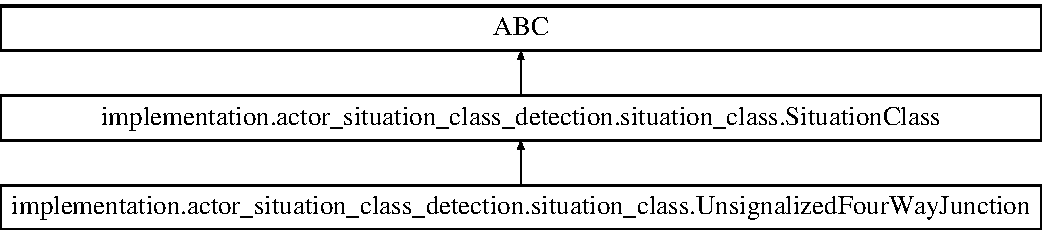
\includegraphics[height=3.000000cm]{classimplementation_1_1actor__situation__class__detection_1_1situation__class_1_1_unsignalized_four_way_junction}
\end{center}
\end{figure}
\subsection*{Public Member Functions}
\begin{DoxyCompactItemize}
\item 
def \hyperlink{classimplementation_1_1actor__situation__class__detection_1_1situation__class_1_1_unsignalized_four_way_junction_a2b3ddd1bcbad64a16e35bbe4ef1e8144}{\+\_\+\+\_\+init\+\_\+\+\_\+} (self, \hyperlink{classimplementation_1_1actor__situation__class__detection_1_1situation__class_1_1_situation_class_a27d4d3259b8bb96107692e2b936ce801}{id}, situation\+\_\+class\+\_\+polygon\+\_\+coordinates)
\item 
def \hyperlink{classimplementation_1_1actor__situation__class__detection_1_1situation__class_1_1_unsignalized_four_way_junction_a0847bd9feb8f04f055599ac084c8228e}{clear\+\_\+actor\+\_\+associations} (self)
\item 
def \hyperlink{classimplementation_1_1actor__situation__class__detection_1_1situation__class_1_1_unsignalized_four_way_junction_a9ac1411f1951cd2b3c989cff2c3e73e4}{update\+\_\+actor\+\_\+association}
\item 
def \hyperlink{classimplementation_1_1actor__situation__class__detection_1_1situation__class_1_1_unsignalized_four_way_junction_a5e0cc68aa2910a3c2b087b5226efec79}{print\+\_\+information}
\end{DoxyCompactItemize}
\subsection*{Additional Inherited Members}


\subsection{Constructor \& Destructor Documentation}
\mbox{\Hypertarget{classimplementation_1_1actor__situation__class__detection_1_1situation__class_1_1_unsignalized_four_way_junction_a2b3ddd1bcbad64a16e35bbe4ef1e8144}\label{classimplementation_1_1actor__situation__class__detection_1_1situation__class_1_1_unsignalized_four_way_junction_a2b3ddd1bcbad64a16e35bbe4ef1e8144}} 
\index{implementation\+::actor\+\_\+situation\+\_\+class\+\_\+detection\+::situation\+\_\+class\+::\+Unsignalized\+Four\+Way\+Junction@{implementation\+::actor\+\_\+situation\+\_\+class\+\_\+detection\+::situation\+\_\+class\+::\+Unsignalized\+Four\+Way\+Junction}!\+\_\+\+\_\+init\+\_\+\+\_\+@{\+\_\+\+\_\+init\+\_\+\+\_\+}}
\index{\+\_\+\+\_\+init\+\_\+\+\_\+@{\+\_\+\+\_\+init\+\_\+\+\_\+}!implementation\+::actor\+\_\+situation\+\_\+class\+\_\+detection\+::situation\+\_\+class\+::\+Unsignalized\+Four\+Way\+Junction@{implementation\+::actor\+\_\+situation\+\_\+class\+\_\+detection\+::situation\+\_\+class\+::\+Unsignalized\+Four\+Way\+Junction}}
\subsubsection{\texorpdfstring{\+\_\+\+\_\+init\+\_\+\+\_\+()}{\_\_init\_\_()}}
{\footnotesize\ttfamily def implementation.\+actor\+\_\+situation\+\_\+class\+\_\+detection.\+situation\+\_\+class.\+Unsignalized\+Four\+Way\+Junction.\+\_\+\+\_\+init\+\_\+\+\_\+ (\begin{DoxyParamCaption}\item[{}]{self,  }\item[{}]{id,  }\item[{}]{situation\+\_\+class\+\_\+polygon\+\_\+coordinates }\end{DoxyParamCaption})}



\subsection{Member Function Documentation}
\mbox{\Hypertarget{classimplementation_1_1actor__situation__class__detection_1_1situation__class_1_1_unsignalized_four_way_junction_a0847bd9feb8f04f055599ac084c8228e}\label{classimplementation_1_1actor__situation__class__detection_1_1situation__class_1_1_unsignalized_four_way_junction_a0847bd9feb8f04f055599ac084c8228e}} 
\index{implementation\+::actor\+\_\+situation\+\_\+class\+\_\+detection\+::situation\+\_\+class\+::\+Unsignalized\+Four\+Way\+Junction@{implementation\+::actor\+\_\+situation\+\_\+class\+\_\+detection\+::situation\+\_\+class\+::\+Unsignalized\+Four\+Way\+Junction}!clear\+\_\+actor\+\_\+associations@{clear\+\_\+actor\+\_\+associations}}
\index{clear\+\_\+actor\+\_\+associations@{clear\+\_\+actor\+\_\+associations}!implementation\+::actor\+\_\+situation\+\_\+class\+\_\+detection\+::situation\+\_\+class\+::\+Unsignalized\+Four\+Way\+Junction@{implementation\+::actor\+\_\+situation\+\_\+class\+\_\+detection\+::situation\+\_\+class\+::\+Unsignalized\+Four\+Way\+Junction}}
\subsubsection{\texorpdfstring{clear\+\_\+actor\+\_\+associations()}{clear\_actor\_associations()}}
{\footnotesize\ttfamily def implementation.\+actor\+\_\+situation\+\_\+class\+\_\+detection.\+situation\+\_\+class.\+Unsignalized\+Four\+Way\+Junction.\+clear\+\_\+actor\+\_\+associations (\begin{DoxyParamCaption}\item[{}]{self }\end{DoxyParamCaption})}

\mbox{\Hypertarget{classimplementation_1_1actor__situation__class__detection_1_1situation__class_1_1_unsignalized_four_way_junction_a5e0cc68aa2910a3c2b087b5226efec79}\label{classimplementation_1_1actor__situation__class__detection_1_1situation__class_1_1_unsignalized_four_way_junction_a5e0cc68aa2910a3c2b087b5226efec79}} 
\index{implementation\+::actor\+\_\+situation\+\_\+class\+\_\+detection\+::situation\+\_\+class\+::\+Unsignalized\+Four\+Way\+Junction@{implementation\+::actor\+\_\+situation\+\_\+class\+\_\+detection\+::situation\+\_\+class\+::\+Unsignalized\+Four\+Way\+Junction}!print\+\_\+information@{print\+\_\+information}}
\index{print\+\_\+information@{print\+\_\+information}!implementation\+::actor\+\_\+situation\+\_\+class\+\_\+detection\+::situation\+\_\+class\+::\+Unsignalized\+Four\+Way\+Junction@{implementation\+::actor\+\_\+situation\+\_\+class\+\_\+detection\+::situation\+\_\+class\+::\+Unsignalized\+Four\+Way\+Junction}}
\subsubsection{\texorpdfstring{print\+\_\+information()}{print\_information()}}
{\footnotesize\ttfamily def implementation.\+actor\+\_\+situation\+\_\+class\+\_\+detection.\+situation\+\_\+class.\+Unsignalized\+Four\+Way\+Junction.\+print\+\_\+information (\begin{DoxyParamCaption}\item[{}]{self,  }\item[{}]{actor }\end{DoxyParamCaption})}

\mbox{\Hypertarget{classimplementation_1_1actor__situation__class__detection_1_1situation__class_1_1_unsignalized_four_way_junction_a9ac1411f1951cd2b3c989cff2c3e73e4}\label{classimplementation_1_1actor__situation__class__detection_1_1situation__class_1_1_unsignalized_four_way_junction_a9ac1411f1951cd2b3c989cff2c3e73e4}} 
\index{implementation\+::actor\+\_\+situation\+\_\+class\+\_\+detection\+::situation\+\_\+class\+::\+Unsignalized\+Four\+Way\+Junction@{implementation\+::actor\+\_\+situation\+\_\+class\+\_\+detection\+::situation\+\_\+class\+::\+Unsignalized\+Four\+Way\+Junction}!update\+\_\+actor\+\_\+association@{update\+\_\+actor\+\_\+association}}
\index{update\+\_\+actor\+\_\+association@{update\+\_\+actor\+\_\+association}!implementation\+::actor\+\_\+situation\+\_\+class\+\_\+detection\+::situation\+\_\+class\+::\+Unsignalized\+Four\+Way\+Junction@{implementation\+::actor\+\_\+situation\+\_\+class\+\_\+detection\+::situation\+\_\+class\+::\+Unsignalized\+Four\+Way\+Junction}}
\subsubsection{\texorpdfstring{update\+\_\+actor\+\_\+association()}{update\_actor\_association()}}
{\footnotesize\ttfamily def implementation.\+actor\+\_\+situation\+\_\+class\+\_\+detection.\+situation\+\_\+class.\+Unsignalized\+Four\+Way\+Junction.\+update\+\_\+actor\+\_\+association (\begin{DoxyParamCaption}\item[{}]{self,  }\item[{}]{actor }\end{DoxyParamCaption})}



The documentation for this class was generated from the following file\+:\begin{DoxyCompactItemize}
\item 
implementation/actor\+\_\+situation\+\_\+class\+\_\+detection/\hyperlink{situation__class_8py}{situation\+\_\+class.\+py}\end{DoxyCompactItemize}

\hypertarget{classimplementation_1_1data__model_1_1positions_1_1_vector3_d}{}\section{implementation.\+data\+\_\+model.\+positions.\+Vector3D Class Reference}
\label{classimplementation_1_1data__model_1_1positions_1_1_vector3_d}\index{implementation.\+data\+\_\+model.\+positions.\+Vector3D@{implementation.\+data\+\_\+model.\+positions.\+Vector3D}}
Inheritance diagram for implementation.\+data\+\_\+model.\+positions.\+Vector3D\+:\begin{figure}[H]
\begin{center}
\leavevmode
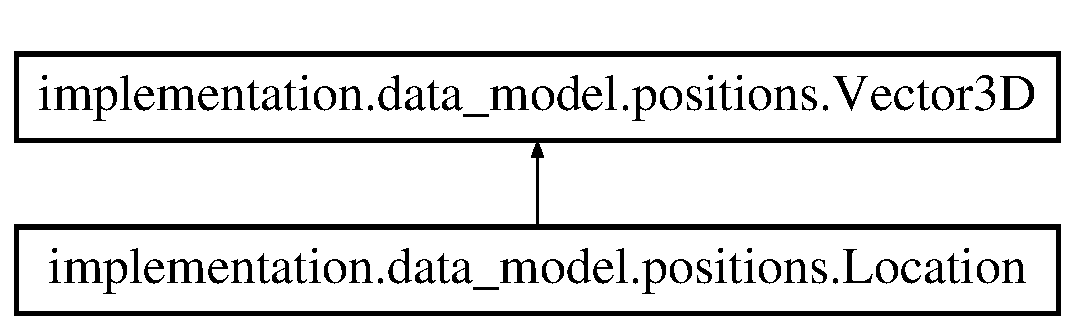
\includegraphics[height=2.000000cm]{classimplementation_1_1data__model_1_1positions_1_1_vector3_d}
\end{center}
\end{figure}
\subsection*{Public Member Functions}
\begin{DoxyCompactItemize}
\item 
def \hyperlink{classimplementation_1_1data__model_1_1positions_1_1_vector3_d_a1f561acdb2feabd9f92441d27fac384c}{invert} (self)
\item 
def \hyperlink{classimplementation_1_1data__model_1_1positions_1_1_vector3_d_a606698a8b72c539e8d8bf3b37946d01f}{\+\_\+\+\_\+add\+\_\+\+\_\+}
\item 
def \hyperlink{classimplementation_1_1data__model_1_1positions_1_1_vector3_d_a7c1d2d39ec8d81ad5d571007cf27fb90}{\+\_\+\+\_\+sub\+\_\+\+\_\+}
\item 
def \hyperlink{classimplementation_1_1data__model_1_1positions_1_1_vector3_d_a1d4b507104453004f32a53274a7f961d}{\+\_\+\+\_\+mul\+\_\+\+\_\+}
\item 
def \hyperlink{classimplementation_1_1data__model_1_1positions_1_1_vector3_d_ad728a8b5918c160cc048f5d80e596da5}{\+\_\+\+\_\+iter\+\_\+\+\_\+} (self)
\end{DoxyCompactItemize}
\subsection*{Static Public Attributes}
\begin{DoxyCompactItemize}
\item 
\hyperlink{classimplementation_1_1data__model_1_1positions_1_1_vector3_d_abb66fd44140d7eb3a383cdf27685741f}{float}
\end{DoxyCompactItemize}


\subsection{Member Function Documentation}
\mbox{\Hypertarget{classimplementation_1_1data__model_1_1positions_1_1_vector3_d_a606698a8b72c539e8d8bf3b37946d01f}\label{classimplementation_1_1data__model_1_1positions_1_1_vector3_d_a606698a8b72c539e8d8bf3b37946d01f}} 
\index{implementation\+::data\+\_\+model\+::positions\+::\+Vector3D@{implementation\+::data\+\_\+model\+::positions\+::\+Vector3D}!\+\_\+\+\_\+add\+\_\+\+\_\+@{\+\_\+\+\_\+add\+\_\+\+\_\+}}
\index{\+\_\+\+\_\+add\+\_\+\+\_\+@{\+\_\+\+\_\+add\+\_\+\+\_\+}!implementation\+::data\+\_\+model\+::positions\+::\+Vector3D@{implementation\+::data\+\_\+model\+::positions\+::\+Vector3D}}
\subsubsection{\texorpdfstring{\+\_\+\+\_\+add\+\_\+\+\_\+()}{\_\_add\_\_()}}
{\footnotesize\ttfamily def implementation.\+data\+\_\+model.\+positions.\+Vector3\+D.\+\_\+\+\_\+add\+\_\+\+\_\+ (\begin{DoxyParamCaption}\item[{}]{self,  }\item[{}]{other\+\_\+location }\end{DoxyParamCaption})}

\mbox{\Hypertarget{classimplementation_1_1data__model_1_1positions_1_1_vector3_d_ad728a8b5918c160cc048f5d80e596da5}\label{classimplementation_1_1data__model_1_1positions_1_1_vector3_d_ad728a8b5918c160cc048f5d80e596da5}} 
\index{implementation\+::data\+\_\+model\+::positions\+::\+Vector3D@{implementation\+::data\+\_\+model\+::positions\+::\+Vector3D}!\+\_\+\+\_\+iter\+\_\+\+\_\+@{\+\_\+\+\_\+iter\+\_\+\+\_\+}}
\index{\+\_\+\+\_\+iter\+\_\+\+\_\+@{\+\_\+\+\_\+iter\+\_\+\+\_\+}!implementation\+::data\+\_\+model\+::positions\+::\+Vector3D@{implementation\+::data\+\_\+model\+::positions\+::\+Vector3D}}
\subsubsection{\texorpdfstring{\+\_\+\+\_\+iter\+\_\+\+\_\+()}{\_\_iter\_\_()}}
{\footnotesize\ttfamily def implementation.\+data\+\_\+model.\+positions.\+Vector3\+D.\+\_\+\+\_\+iter\+\_\+\+\_\+ (\begin{DoxyParamCaption}\item[{}]{self }\end{DoxyParamCaption})}

\mbox{\Hypertarget{classimplementation_1_1data__model_1_1positions_1_1_vector3_d_a1d4b507104453004f32a53274a7f961d}\label{classimplementation_1_1data__model_1_1positions_1_1_vector3_d_a1d4b507104453004f32a53274a7f961d}} 
\index{implementation\+::data\+\_\+model\+::positions\+::\+Vector3D@{implementation\+::data\+\_\+model\+::positions\+::\+Vector3D}!\+\_\+\+\_\+mul\+\_\+\+\_\+@{\+\_\+\+\_\+mul\+\_\+\+\_\+}}
\index{\+\_\+\+\_\+mul\+\_\+\+\_\+@{\+\_\+\+\_\+mul\+\_\+\+\_\+}!implementation\+::data\+\_\+model\+::positions\+::\+Vector3D@{implementation\+::data\+\_\+model\+::positions\+::\+Vector3D}}
\subsubsection{\texorpdfstring{\+\_\+\+\_\+mul\+\_\+\+\_\+()}{\_\_mul\_\_()}}
{\footnotesize\ttfamily def implementation.\+data\+\_\+model.\+positions.\+Vector3\+D.\+\_\+\+\_\+mul\+\_\+\+\_\+ (\begin{DoxyParamCaption}\item[{}]{self,  }\item[{}]{other }\end{DoxyParamCaption})}

\mbox{\Hypertarget{classimplementation_1_1data__model_1_1positions_1_1_vector3_d_a7c1d2d39ec8d81ad5d571007cf27fb90}\label{classimplementation_1_1data__model_1_1positions_1_1_vector3_d_a7c1d2d39ec8d81ad5d571007cf27fb90}} 
\index{implementation\+::data\+\_\+model\+::positions\+::\+Vector3D@{implementation\+::data\+\_\+model\+::positions\+::\+Vector3D}!\+\_\+\+\_\+sub\+\_\+\+\_\+@{\+\_\+\+\_\+sub\+\_\+\+\_\+}}
\index{\+\_\+\+\_\+sub\+\_\+\+\_\+@{\+\_\+\+\_\+sub\+\_\+\+\_\+}!implementation\+::data\+\_\+model\+::positions\+::\+Vector3D@{implementation\+::data\+\_\+model\+::positions\+::\+Vector3D}}
\subsubsection{\texorpdfstring{\+\_\+\+\_\+sub\+\_\+\+\_\+()}{\_\_sub\_\_()}}
{\footnotesize\ttfamily def implementation.\+data\+\_\+model.\+positions.\+Vector3\+D.\+\_\+\+\_\+sub\+\_\+\+\_\+ (\begin{DoxyParamCaption}\item[{}]{self,  }\item[{}]{other\+\_\+location }\end{DoxyParamCaption})}

\mbox{\Hypertarget{classimplementation_1_1data__model_1_1positions_1_1_vector3_d_a1f561acdb2feabd9f92441d27fac384c}\label{classimplementation_1_1data__model_1_1positions_1_1_vector3_d_a1f561acdb2feabd9f92441d27fac384c}} 
\index{implementation\+::data\+\_\+model\+::positions\+::\+Vector3D@{implementation\+::data\+\_\+model\+::positions\+::\+Vector3D}!invert@{invert}}
\index{invert@{invert}!implementation\+::data\+\_\+model\+::positions\+::\+Vector3D@{implementation\+::data\+\_\+model\+::positions\+::\+Vector3D}}
\subsubsection{\texorpdfstring{invert()}{invert()}}
{\footnotesize\ttfamily def implementation.\+data\+\_\+model.\+positions.\+Vector3\+D.\+invert (\begin{DoxyParamCaption}\item[{}]{self,  }\item[{}]{Vector3D }\end{DoxyParamCaption})}

\begin{DoxyVerb}Returns the inverted Vector

Returns
-------
Vector3D
    Inverted Vector\end{DoxyVerb}
 

\subsection{Member Data Documentation}
\mbox{\Hypertarget{classimplementation_1_1data__model_1_1positions_1_1_vector3_d_abb66fd44140d7eb3a383cdf27685741f}\label{classimplementation_1_1data__model_1_1positions_1_1_vector3_d_abb66fd44140d7eb3a383cdf27685741f}} 
\index{implementation\+::data\+\_\+model\+::positions\+::\+Vector3D@{implementation\+::data\+\_\+model\+::positions\+::\+Vector3D}!float@{float}}
\index{float@{float}!implementation\+::data\+\_\+model\+::positions\+::\+Vector3D@{implementation\+::data\+\_\+model\+::positions\+::\+Vector3D}}
\subsubsection{\texorpdfstring{float}{float}}
{\footnotesize\ttfamily implementation.\+data\+\_\+model.\+positions.\+Vector3\+D.\+float\hspace{0.3cm}{\ttfamily [static]}}



The documentation for this class was generated from the following file\+:\begin{DoxyCompactItemize}
\item 
implementation/data\+\_\+model/\hyperlink{positions_8py}{positions.\+py}\end{DoxyCompactItemize}

\hypertarget{classimplementation_1_1data__model_1_1vehicle_1_1_vehicle}{}\section{implementation.\+data\+\_\+model.\+vehicle.\+Vehicle Class Reference}
\label{classimplementation_1_1data__model_1_1vehicle_1_1_vehicle}\index{implementation.\+data\+\_\+model.\+vehicle.\+Vehicle@{implementation.\+data\+\_\+model.\+vehicle.\+Vehicle}}
Inheritance diagram for implementation.\+data\+\_\+model.\+vehicle.\+Vehicle\+:\begin{figure}[H]
\begin{center}
\leavevmode
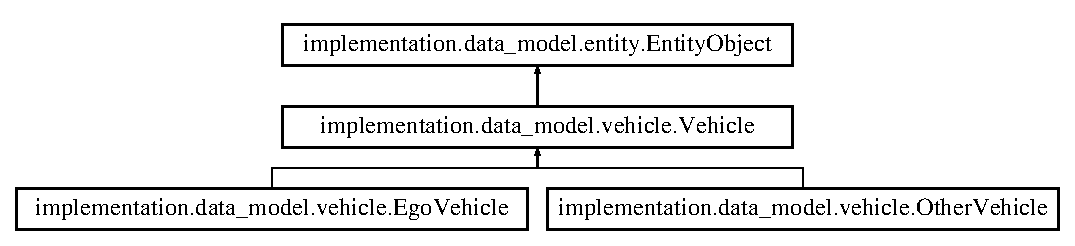
\includegraphics[height=2.857143cm]{classimplementation_1_1data__model_1_1vehicle_1_1_vehicle}
\end{center}
\end{figure}
\subsection*{Public Member Functions}
\begin{DoxyCompactItemize}
\item 
def \hyperlink{classimplementation_1_1data__model_1_1vehicle_1_1_vehicle_a2155a545440eae609b8e4900d5cbd2f8}{get\+\_\+middle\+\_\+points\+\_\+dict}
\item 
def \hyperlink{classimplementation_1_1data__model_1_1vehicle_1_1_vehicle_ab2e31dc51c68d50d066364def03ef99c}{get\+\_\+acceleration\+\_\+vector} (self)
\item 
def \hyperlink{classimplementation_1_1data__model_1_1vehicle_1_1_vehicle_aa96b1b4dfa57da623a79a711011a6113}{get\+\_\+velocity} (self)
\item 
def \hyperlink{classimplementation_1_1data__model_1_1vehicle_1_1_vehicle_a9252c162137f564dfcec306c08f22eba}{\+\_\+\+\_\+hash\+\_\+\+\_\+} (self)
\end{DoxyCompactItemize}
\subsection*{Static Public Attributes}
\begin{DoxyCompactItemize}
\item 
\hyperlink{classimplementation_1_1data__model_1_1vehicle_1_1_vehicle_aa942b836bd6fa833c5d3789b10c2ada5}{int}
\item 
\hyperlink{classimplementation_1_1data__model_1_1vehicle_1_1_vehicle_a05d792fb397d5ec7acb7335449622f2f}{str}
\item 
\hyperlink{classimplementation_1_1data__model_1_1vehicle_1_1_vehicle_a2f5cd50538d2080f651dd154c1597e80}{float}
\item 
\hyperlink{classimplementation_1_1data__model_1_1vehicle_1_1_vehicle_a3530d8bb1b04006bec3e363071b2b87d}{Vehicle\+Light\+State}
\item 
\hyperlink{classimplementation_1_1data__model_1_1vehicle_1_1_vehicle_ad98d81e5e18f2fbd49fd20056d9fb43d}{Vehicle\+Control}
\item 
\hyperlink{classimplementation_1_1data__model_1_1vehicle_1_1_vehicle_a5c505c6d69ccd0737d00d1bc203f78cc}{Vehicle\+Category}
\end{DoxyCompactItemize}


\subsection{Member Function Documentation}
\mbox{\Hypertarget{classimplementation_1_1data__model_1_1vehicle_1_1_vehicle_a9252c162137f564dfcec306c08f22eba}\label{classimplementation_1_1data__model_1_1vehicle_1_1_vehicle_a9252c162137f564dfcec306c08f22eba}} 
\index{implementation\+::data\+\_\+model\+::vehicle\+::\+Vehicle@{implementation\+::data\+\_\+model\+::vehicle\+::\+Vehicle}!\+\_\+\+\_\+hash\+\_\+\+\_\+@{\+\_\+\+\_\+hash\+\_\+\+\_\+}}
\index{\+\_\+\+\_\+hash\+\_\+\+\_\+@{\+\_\+\+\_\+hash\+\_\+\+\_\+}!implementation\+::data\+\_\+model\+::vehicle\+::\+Vehicle@{implementation\+::data\+\_\+model\+::vehicle\+::\+Vehicle}}
\subsubsection{\texorpdfstring{\+\_\+\+\_\+hash\+\_\+\+\_\+()}{\_\_hash\_\_()}}
{\footnotesize\ttfamily def implementation.\+data\+\_\+model.\+vehicle.\+Vehicle.\+\_\+\+\_\+hash\+\_\+\+\_\+ (\begin{DoxyParamCaption}\item[{}]{self }\end{DoxyParamCaption})}

\mbox{\Hypertarget{classimplementation_1_1data__model_1_1vehicle_1_1_vehicle_ab2e31dc51c68d50d066364def03ef99c}\label{classimplementation_1_1data__model_1_1vehicle_1_1_vehicle_ab2e31dc51c68d50d066364def03ef99c}} 
\index{implementation\+::data\+\_\+model\+::vehicle\+::\+Vehicle@{implementation\+::data\+\_\+model\+::vehicle\+::\+Vehicle}!get\+\_\+acceleration\+\_\+vector@{get\+\_\+acceleration\+\_\+vector}}
\index{get\+\_\+acceleration\+\_\+vector@{get\+\_\+acceleration\+\_\+vector}!implementation\+::data\+\_\+model\+::vehicle\+::\+Vehicle@{implementation\+::data\+\_\+model\+::vehicle\+::\+Vehicle}}
\subsubsection{\texorpdfstring{get\+\_\+acceleration\+\_\+vector()}{get\_acceleration\_vector()}}
{\footnotesize\ttfamily def implementation.\+data\+\_\+model.\+vehicle.\+Vehicle.\+get\+\_\+acceleration\+\_\+vector (\begin{DoxyParamCaption}\item[{}]{self,  }\item[{}]{Vector3D }\end{DoxyParamCaption})}

\mbox{\Hypertarget{classimplementation_1_1data__model_1_1vehicle_1_1_vehicle_a2155a545440eae609b8e4900d5cbd2f8}\label{classimplementation_1_1data__model_1_1vehicle_1_1_vehicle_a2155a545440eae609b8e4900d5cbd2f8}} 
\index{implementation\+::data\+\_\+model\+::vehicle\+::\+Vehicle@{implementation\+::data\+\_\+model\+::vehicle\+::\+Vehicle}!get\+\_\+middle\+\_\+points\+\_\+dict@{get\+\_\+middle\+\_\+points\+\_\+dict}}
\index{get\+\_\+middle\+\_\+points\+\_\+dict@{get\+\_\+middle\+\_\+points\+\_\+dict}!implementation\+::data\+\_\+model\+::vehicle\+::\+Vehicle@{implementation\+::data\+\_\+model\+::vehicle\+::\+Vehicle}}
\subsubsection{\texorpdfstring{get\+\_\+middle\+\_\+points\+\_\+dict()}{get\_middle\_points\_dict()}}
{\footnotesize\ttfamily def implementation.\+data\+\_\+model.\+vehicle.\+Vehicle.\+get\+\_\+middle\+\_\+points\+\_\+dict (\begin{DoxyParamCaption}\item[{}]{self,  }\item[{}]{vehicle\+\_\+world\+\_\+position }\end{DoxyParamCaption})}

\mbox{\Hypertarget{classimplementation_1_1data__model_1_1vehicle_1_1_vehicle_aa96b1b4dfa57da623a79a711011a6113}\label{classimplementation_1_1data__model_1_1vehicle_1_1_vehicle_aa96b1b4dfa57da623a79a711011a6113}} 
\index{implementation\+::data\+\_\+model\+::vehicle\+::\+Vehicle@{implementation\+::data\+\_\+model\+::vehicle\+::\+Vehicle}!get\+\_\+velocity@{get\+\_\+velocity}}
\index{get\+\_\+velocity@{get\+\_\+velocity}!implementation\+::data\+\_\+model\+::vehicle\+::\+Vehicle@{implementation\+::data\+\_\+model\+::vehicle\+::\+Vehicle}}
\subsubsection{\texorpdfstring{get\+\_\+velocity()}{get\_velocity()}}
{\footnotesize\ttfamily def implementation.\+data\+\_\+model.\+vehicle.\+Vehicle.\+get\+\_\+velocity (\begin{DoxyParamCaption}\item[{}]{self,  }\item[{}]{Vector3D }\end{DoxyParamCaption})}



\subsection{Member Data Documentation}
\mbox{\Hypertarget{classimplementation_1_1data__model_1_1vehicle_1_1_vehicle_a2f5cd50538d2080f651dd154c1597e80}\label{classimplementation_1_1data__model_1_1vehicle_1_1_vehicle_a2f5cd50538d2080f651dd154c1597e80}} 
\index{implementation\+::data\+\_\+model\+::vehicle\+::\+Vehicle@{implementation\+::data\+\_\+model\+::vehicle\+::\+Vehicle}!float@{float}}
\index{float@{float}!implementation\+::data\+\_\+model\+::vehicle\+::\+Vehicle@{implementation\+::data\+\_\+model\+::vehicle\+::\+Vehicle}}
\subsubsection{\texorpdfstring{float}{float}}
{\footnotesize\ttfamily implementation.\+data\+\_\+model.\+vehicle.\+Vehicle.\+float\hspace{0.3cm}{\ttfamily [static]}}

\mbox{\Hypertarget{classimplementation_1_1data__model_1_1vehicle_1_1_vehicle_aa942b836bd6fa833c5d3789b10c2ada5}\label{classimplementation_1_1data__model_1_1vehicle_1_1_vehicle_aa942b836bd6fa833c5d3789b10c2ada5}} 
\index{implementation\+::data\+\_\+model\+::vehicle\+::\+Vehicle@{implementation\+::data\+\_\+model\+::vehicle\+::\+Vehicle}!int@{int}}
\index{int@{int}!implementation\+::data\+\_\+model\+::vehicle\+::\+Vehicle@{implementation\+::data\+\_\+model\+::vehicle\+::\+Vehicle}}
\subsubsection{\texorpdfstring{int}{int}}
{\footnotesize\ttfamily implementation.\+data\+\_\+model.\+vehicle.\+Vehicle.\+int\hspace{0.3cm}{\ttfamily [static]}}

\mbox{\Hypertarget{classimplementation_1_1data__model_1_1vehicle_1_1_vehicle_a05d792fb397d5ec7acb7335449622f2f}\label{classimplementation_1_1data__model_1_1vehicle_1_1_vehicle_a05d792fb397d5ec7acb7335449622f2f}} 
\index{implementation\+::data\+\_\+model\+::vehicle\+::\+Vehicle@{implementation\+::data\+\_\+model\+::vehicle\+::\+Vehicle}!str@{str}}
\index{str@{str}!implementation\+::data\+\_\+model\+::vehicle\+::\+Vehicle@{implementation\+::data\+\_\+model\+::vehicle\+::\+Vehicle}}
\subsubsection{\texorpdfstring{str}{str}}
{\footnotesize\ttfamily implementation.\+data\+\_\+model.\+vehicle.\+Vehicle.\+str\hspace{0.3cm}{\ttfamily [static]}}

\mbox{\Hypertarget{classimplementation_1_1data__model_1_1vehicle_1_1_vehicle_a5c505c6d69ccd0737d00d1bc203f78cc}\label{classimplementation_1_1data__model_1_1vehicle_1_1_vehicle_a5c505c6d69ccd0737d00d1bc203f78cc}} 
\index{implementation\+::data\+\_\+model\+::vehicle\+::\+Vehicle@{implementation\+::data\+\_\+model\+::vehicle\+::\+Vehicle}!Vehicle\+Category@{Vehicle\+Category}}
\index{Vehicle\+Category@{Vehicle\+Category}!implementation\+::data\+\_\+model\+::vehicle\+::\+Vehicle@{implementation\+::data\+\_\+model\+::vehicle\+::\+Vehicle}}
\subsubsection{\texorpdfstring{Vehicle\+Category}{VehicleCategory}}
{\footnotesize\ttfamily implementation.\+data\+\_\+model.\+vehicle.\+Vehicle.\+Vehicle\+Category\hspace{0.3cm}{\ttfamily [static]}}

\mbox{\Hypertarget{classimplementation_1_1data__model_1_1vehicle_1_1_vehicle_ad98d81e5e18f2fbd49fd20056d9fb43d}\label{classimplementation_1_1data__model_1_1vehicle_1_1_vehicle_ad98d81e5e18f2fbd49fd20056d9fb43d}} 
\index{implementation\+::data\+\_\+model\+::vehicle\+::\+Vehicle@{implementation\+::data\+\_\+model\+::vehicle\+::\+Vehicle}!Vehicle\+Control@{Vehicle\+Control}}
\index{Vehicle\+Control@{Vehicle\+Control}!implementation\+::data\+\_\+model\+::vehicle\+::\+Vehicle@{implementation\+::data\+\_\+model\+::vehicle\+::\+Vehicle}}
\subsubsection{\texorpdfstring{Vehicle\+Control}{VehicleControl}}
{\footnotesize\ttfamily implementation.\+data\+\_\+model.\+vehicle.\+Vehicle.\+Vehicle\+Control\hspace{0.3cm}{\ttfamily [static]}}

\mbox{\Hypertarget{classimplementation_1_1data__model_1_1vehicle_1_1_vehicle_a3530d8bb1b04006bec3e363071b2b87d}\label{classimplementation_1_1data__model_1_1vehicle_1_1_vehicle_a3530d8bb1b04006bec3e363071b2b87d}} 
\index{implementation\+::data\+\_\+model\+::vehicle\+::\+Vehicle@{implementation\+::data\+\_\+model\+::vehicle\+::\+Vehicle}!Vehicle\+Light\+State@{Vehicle\+Light\+State}}
\index{Vehicle\+Light\+State@{Vehicle\+Light\+State}!implementation\+::data\+\_\+model\+::vehicle\+::\+Vehicle@{implementation\+::data\+\_\+model\+::vehicle\+::\+Vehicle}}
\subsubsection{\texorpdfstring{Vehicle\+Light\+State}{VehicleLightState}}
{\footnotesize\ttfamily implementation.\+data\+\_\+model.\+vehicle.\+Vehicle.\+Vehicle\+Light\+State\hspace{0.3cm}{\ttfamily [static]}}



The documentation for this class was generated from the following file\+:\begin{DoxyCompactItemize}
\item 
implementation/data\+\_\+model/\hyperlink{vehicle_8py}{vehicle.\+py}\end{DoxyCompactItemize}

\hypertarget{classimplementation_1_1actor__situation__class__detection_1_1vehicle__actor__wrapper_1_1_vehicle_actor_wrapper}{}\doxysection{implementation.\+actor\+\_\+situation\+\_\+class\+\_\+detection.\+vehicle\+\_\+actor\+\_\+wrapper.\+Vehicle\+Actor\+Wrapper Class Reference}
\label{classimplementation_1_1actor__situation__class__detection_1_1vehicle__actor__wrapper_1_1_vehicle_actor_wrapper}\index{implementation.actor\_situation\_class\_detection.vehicle\_actor\_wrapper.VehicleActorWrapper@{implementation.actor\_situation\_class\_detection.vehicle\_actor\_wrapper.VehicleActorWrapper}}
Inheritance diagram for implementation.\+actor\+\_\+situation\+\_\+class\+\_\+detection.\+vehicle\+\_\+actor\+\_\+wrapper.\+Vehicle\+Actor\+Wrapper\+:\begin{figure}[H]
\begin{center}
\leavevmode
\includegraphics[height=2.000000cm]{classimplementation_1_1actor__situation__class__detection_1_1vehicle__actor__wrapper_1_1_vehicle_actor_wrapper}
\end{center}
\end{figure}
\doxysubsection*{Public Member Functions}
\begin{DoxyCompactItemize}
\item 
def \mbox{\hyperlink{classimplementation_1_1actor__situation__class__detection_1_1vehicle__actor__wrapper_1_1_vehicle_actor_wrapper_aa9ba440c4a8a4cef9764033073db67d0}{\+\_\+\+\_\+init\+\_\+\+\_\+}} (self, carla.\+Vehicle \mbox{\hyperlink{classimplementation_1_1actor__situation__class__detection_1_1vehicle__actor__wrapper_1_1_vehicle_actor_wrapper_a883123671cd96e9d6bb8072119c64608}{vehicle}})
\item 
def \mbox{\hyperlink{classimplementation_1_1actor__situation__class__detection_1_1vehicle__actor__wrapper_1_1_vehicle_actor_wrapper_af7077301cef97b0b4842c9d4c221640b}{role\+\_\+name}} (self)
\item 
def \mbox{\hyperlink{classimplementation_1_1actor__situation__class__detection_1_1vehicle__actor__wrapper_1_1_vehicle_actor_wrapper_a8833bbb1a122a4aba1aced7d3f7c6530}{id}} (self)
\item 
def \mbox{\hyperlink{classimplementation_1_1actor__situation__class__detection_1_1vehicle__actor__wrapper_1_1_vehicle_actor_wrapper_a20beab7a17865630337d1d3797552a17}{transform}} (self)
\item 
def \mbox{\hyperlink{classimplementation_1_1actor__situation__class__detection_1_1vehicle__actor__wrapper_1_1_vehicle_actor_wrapper_a0e913c295c7f4276b0f71144aa0c7e43}{forward\+\_\+vector}} (self)
\item 
(Polygon, List\mbox{[}\char`\"{}Line\+String\char`\"{}\mbox{]}) \mbox{\hyperlink{classimplementation_1_1actor__situation__class__detection_1_1vehicle__actor__wrapper_1_1_vehicle_actor_wrapper_a5c6c97c4ac3b889384be6ed56c4e52d6}{get\+\_\+front\+\_\+sensing\+\_\+area}} (self, carla.\+Map carla\+\_\+map)
\item 
(Polygon, List\mbox{[}\char`\"{}Line\+String\char`\"{}\mbox{]}) \mbox{\hyperlink{classimplementation_1_1actor__situation__class__detection_1_1vehicle__actor__wrapper_1_1_vehicle_actor_wrapper_a128aad88b915e589955235717439f2e7}{get\+\_\+side\+\_\+sensing\+\_\+area}} (self, carla.\+Map carla\+\_\+map, \mbox{\hyperlink{classimplementation_1_1actor__situation__class__detection_1_1vehicle__actor__wrapper_1_1_vehicle_point_id}{Vehicle\+Point\+Id}} side\+\_\+vehicle\+\_\+point\+\_\+id)
\item 
List\mbox{[}\char`\"{}Point\char`\"{}\mbox{]} \mbox{\hyperlink{classimplementation_1_1actor__situation__class__detection_1_1vehicle__actor__wrapper_1_1_vehicle_actor_wrapper_adabf738f94c19c1d6972073fb0905896}{get\+\_\+rear\+\_\+mid\+\_\+center\+\_\+linestring\+\_\+points}} (self)
\end{DoxyCompactItemize}
\doxysubsection*{Public Attributes}
\begin{DoxyCompactItemize}
\item 
\mbox{\hyperlink{classimplementation_1_1actor__situation__class__detection_1_1vehicle__actor__wrapper_1_1_vehicle_actor_wrapper_a883123671cd96e9d6bb8072119c64608}{vehicle}}
\item 
\mbox{\hyperlink{classimplementation_1_1actor__situation__class__detection_1_1vehicle__actor__wrapper_1_1_vehicle_actor_wrapper_a2d5984ba61d90743c38ba6f69ebe6805}{vehicle\+\_\+points}}
\end{DoxyCompactItemize}


\doxysubsection{Detailed Description}
\begin{DoxyVerb}Wrapper class for a carla.Vehicle object. The carla.Vehicle object can be accessed through the vehicle attribute.

Attributes
----------
vehicle: carla.Vehicle
    carla.Vehicle object that is wrapped within this object.
vehicle_points: Dict[VehiclePointId, carla.Vector3D]
    Wrapped vehicle actors that are on the right lane\end{DoxyVerb}
 

\doxysubsection{Constructor \& Destructor Documentation}
\mbox{\Hypertarget{classimplementation_1_1actor__situation__class__detection_1_1vehicle__actor__wrapper_1_1_vehicle_actor_wrapper_aa9ba440c4a8a4cef9764033073db67d0}\label{classimplementation_1_1actor__situation__class__detection_1_1vehicle__actor__wrapper_1_1_vehicle_actor_wrapper_aa9ba440c4a8a4cef9764033073db67d0}} 
\index{implementation.actor\_situation\_class\_detection.vehicle\_actor\_wrapper.VehicleActorWrapper@{implementation.actor\_situation\_class\_detection.vehicle\_actor\_wrapper.VehicleActorWrapper}!\_\_init\_\_@{\_\_init\_\_}}
\index{\_\_init\_\_@{\_\_init\_\_}!implementation.actor\_situation\_class\_detection.vehicle\_actor\_wrapper.VehicleActorWrapper@{implementation.actor\_situation\_class\_detection.vehicle\_actor\_wrapper.VehicleActorWrapper}}
\doxysubsubsection{\texorpdfstring{\_\_init\_\_()}{\_\_init\_\_()}}
{\footnotesize\ttfamily def implementation.\+actor\+\_\+situation\+\_\+class\+\_\+detection.\+vehicle\+\_\+actor\+\_\+wrapper.\+Vehicle\+Actor\+Wrapper.\+\_\+\+\_\+init\+\_\+\+\_\+ (\begin{DoxyParamCaption}\item[{}]{self,  }\item[{carla.\+Vehicle}]{vehicle }\end{DoxyParamCaption})}



\doxysubsection{Member Function Documentation}
\mbox{\Hypertarget{classimplementation_1_1actor__situation__class__detection_1_1vehicle__actor__wrapper_1_1_vehicle_actor_wrapper_a0e913c295c7f4276b0f71144aa0c7e43}\label{classimplementation_1_1actor__situation__class__detection_1_1vehicle__actor__wrapper_1_1_vehicle_actor_wrapper_a0e913c295c7f4276b0f71144aa0c7e43}} 
\index{implementation.actor\_situation\_class\_detection.vehicle\_actor\_wrapper.VehicleActorWrapper@{implementation.actor\_situation\_class\_detection.vehicle\_actor\_wrapper.VehicleActorWrapper}!forward\_vector@{forward\_vector}}
\index{forward\_vector@{forward\_vector}!implementation.actor\_situation\_class\_detection.vehicle\_actor\_wrapper.VehicleActorWrapper@{implementation.actor\_situation\_class\_detection.vehicle\_actor\_wrapper.VehicleActorWrapper}}
\doxysubsubsection{\texorpdfstring{forward\_vector()}{forward\_vector()}}
{\footnotesize\ttfamily def implementation.\+actor\+\_\+situation\+\_\+class\+\_\+detection.\+vehicle\+\_\+actor\+\_\+wrapper.\+Vehicle\+Actor\+Wrapper.\+forward\+\_\+vector (\begin{DoxyParamCaption}\item[{}]{self }\end{DoxyParamCaption})}

\begin{DoxyVerb}Retrieves the forward vector as carla.Vector3D object of the wrapped carla.Vehicle object\end{DoxyVerb}
 \mbox{\Hypertarget{classimplementation_1_1actor__situation__class__detection_1_1vehicle__actor__wrapper_1_1_vehicle_actor_wrapper_a5c6c97c4ac3b889384be6ed56c4e52d6}\label{classimplementation_1_1actor__situation__class__detection_1_1vehicle__actor__wrapper_1_1_vehicle_actor_wrapper_a5c6c97c4ac3b889384be6ed56c4e52d6}} 
\index{implementation.actor\_situation\_class\_detection.vehicle\_actor\_wrapper.VehicleActorWrapper@{implementation.actor\_situation\_class\_detection.vehicle\_actor\_wrapper.VehicleActorWrapper}!get\_front\_sensing\_area@{get\_front\_sensing\_area}}
\index{get\_front\_sensing\_area@{get\_front\_sensing\_area}!implementation.actor\_situation\_class\_detection.vehicle\_actor\_wrapper.VehicleActorWrapper@{implementation.actor\_situation\_class\_detection.vehicle\_actor\_wrapper.VehicleActorWrapper}}
\doxysubsubsection{\texorpdfstring{get\_front\_sensing\_area()}{get\_front\_sensing\_area()}}
{\footnotesize\ttfamily  (Polygon, List\mbox{[}\char`\"{}Line\+String\char`\"{}\mbox{]}) implementation.\+actor\+\_\+situation\+\_\+class\+\_\+detection.\+vehicle\+\_\+actor\+\_\+wrapper.\+Vehicle\+Actor\+Wrapper.\+get\+\_\+front\+\_\+sensing\+\_\+area (\begin{DoxyParamCaption}\item[{}]{self,  }\item[{carla.\+Map}]{carla\+\_\+map }\end{DoxyParamCaption})}

\begin{DoxyVerb}Determines front sensing area for this vehicle using the configuration parameter
FRONT_SENSING_DISTANCE_TIME_GAP_IN_SECONDS. Returns front sensing area as shapely.geometry.Polygon object.
If configuration parameter DEBUG_MODE is set to true, this method additionally returns the lines of the polygon
as a list of shapely.geometry.LineString objects for visualization in carla.

Parameters
----------
carla_map: carla.Map
    Map object to obtain way points for sensing area calculation

Returns
-------
Polygon
    A shapely.geometry.Polygon object that defines the front sensing area
List[LineString]
    A list of shapely.geometry.LineString objects that represent the edges of the front sensing area.
    The line strings are only needed for drawing debug lines of the sensing area on the Carla server. Therefore
    the list is only returned if DEBUG_MODE flag is set to True. Otherwise None is returned instead.
\end{DoxyVerb}
 \mbox{\Hypertarget{classimplementation_1_1actor__situation__class__detection_1_1vehicle__actor__wrapper_1_1_vehicle_actor_wrapper_adabf738f94c19c1d6972073fb0905896}\label{classimplementation_1_1actor__situation__class__detection_1_1vehicle__actor__wrapper_1_1_vehicle_actor_wrapper_adabf738f94c19c1d6972073fb0905896}} 
\index{implementation.actor\_situation\_class\_detection.vehicle\_actor\_wrapper.VehicleActorWrapper@{implementation.actor\_situation\_class\_detection.vehicle\_actor\_wrapper.VehicleActorWrapper}!get\_rear\_mid\_center\_linestring\_points@{get\_rear\_mid\_center\_linestring\_points}}
\index{get\_rear\_mid\_center\_linestring\_points@{get\_rear\_mid\_center\_linestring\_points}!implementation.actor\_situation\_class\_detection.vehicle\_actor\_wrapper.VehicleActorWrapper@{implementation.actor\_situation\_class\_detection.vehicle\_actor\_wrapper.VehicleActorWrapper}}
\doxysubsubsection{\texorpdfstring{get\_rear\_mid\_center\_linestring\_points()}{get\_rear\_mid\_center\_linestring\_points()}}
{\footnotesize\ttfamily  List\mbox{[}\char`\"{}Point\char`\"{}\mbox{]} implementation.\+actor\+\_\+situation\+\_\+class\+\_\+detection.\+vehicle\+\_\+actor\+\_\+wrapper.\+Vehicle\+Actor\+Wrapper.\+get\+\_\+rear\+\_\+mid\+\_\+center\+\_\+linestring\+\_\+points (\begin{DoxyParamCaption}\item[{}]{self }\end{DoxyParamCaption})}

\begin{DoxyVerb}Method is used for drawing debug lines. It returns a tuple of two points. First is located above and
second is located beneath the rear center point of the vehicle.

Returns
-------
List[Point]
    A tuple of shapely.geometry.Point objects, where the first point is located above
    and the second is located beneath the rear center point of the vehicle.
\end{DoxyVerb}
 \mbox{\Hypertarget{classimplementation_1_1actor__situation__class__detection_1_1vehicle__actor__wrapper_1_1_vehicle_actor_wrapper_a128aad88b915e589955235717439f2e7}\label{classimplementation_1_1actor__situation__class__detection_1_1vehicle__actor__wrapper_1_1_vehicle_actor_wrapper_a128aad88b915e589955235717439f2e7}} 
\index{implementation.actor\_situation\_class\_detection.vehicle\_actor\_wrapper.VehicleActorWrapper@{implementation.actor\_situation\_class\_detection.vehicle\_actor\_wrapper.VehicleActorWrapper}!get\_side\_sensing\_area@{get\_side\_sensing\_area}}
\index{get\_side\_sensing\_area@{get\_side\_sensing\_area}!implementation.actor\_situation\_class\_detection.vehicle\_actor\_wrapper.VehicleActorWrapper@{implementation.actor\_situation\_class\_detection.vehicle\_actor\_wrapper.VehicleActorWrapper}}
\doxysubsubsection{\texorpdfstring{get\_side\_sensing\_area()}{get\_side\_sensing\_area()}}
{\footnotesize\ttfamily  (Polygon, List\mbox{[}\char`\"{}Line\+String\char`\"{}\mbox{]}) implementation.\+actor\+\_\+situation\+\_\+class\+\_\+detection.\+vehicle\+\_\+actor\+\_\+wrapper.\+Vehicle\+Actor\+Wrapper.\+get\+\_\+side\+\_\+sensing\+\_\+area (\begin{DoxyParamCaption}\item[{}]{self,  }\item[{carla.\+Map}]{carla\+\_\+map,  }\item[{\mbox{\hyperlink{classimplementation_1_1actor__situation__class__detection_1_1vehicle__actor__wrapper_1_1_vehicle_point_id}{Vehicle\+Point\+Id}}
                              }]{side\+\_\+vehicle\+\_\+point\+\_\+id }\end{DoxyParamCaption})}

\begin{DoxyVerb}Determines sensing area next to ego vehicle on other lane. On which side the sensing area is created,
depends on parameter side_vehicle_point_id.

Parameters
----------
carla_map: carla.Map
    Map object to obtain way points for sensing area calculation
side_vehicle_point_id: VehiclePointId
    Center mid location of the vehicle side the sensing area shall be created on.
    Possible values are CENTER_MID_LEFT and CENTER_MID_RIGHT

Returns
-------
Polygon
    A shapely.geometry.Polygon object that defines the side sensing area
List[LineString]
    A list of shapely.geometry.LineString objects that represent the edges of the side sensing area.
    The line strings are only needed for drawing debug lines of the sensing area on the Carla server. Therefore
    the list is only returned if DEBUG_MODE flag is set to True. Otherwise None is returned instead.
\end{DoxyVerb}
 \mbox{\Hypertarget{classimplementation_1_1actor__situation__class__detection_1_1vehicle__actor__wrapper_1_1_vehicle_actor_wrapper_a8833bbb1a122a4aba1aced7d3f7c6530}\label{classimplementation_1_1actor__situation__class__detection_1_1vehicle__actor__wrapper_1_1_vehicle_actor_wrapper_a8833bbb1a122a4aba1aced7d3f7c6530}} 
\index{implementation.actor\_situation\_class\_detection.vehicle\_actor\_wrapper.VehicleActorWrapper@{implementation.actor\_situation\_class\_detection.vehicle\_actor\_wrapper.VehicleActorWrapper}!id@{id}}
\index{id@{id}!implementation.actor\_situation\_class\_detection.vehicle\_actor\_wrapper.VehicleActorWrapper@{implementation.actor\_situation\_class\_detection.vehicle\_actor\_wrapper.VehicleActorWrapper}}
\doxysubsubsection{\texorpdfstring{id()}{id()}}
{\footnotesize\ttfamily def implementation.\+actor\+\_\+situation\+\_\+class\+\_\+detection.\+vehicle\+\_\+actor\+\_\+wrapper.\+Vehicle\+Actor\+Wrapper.\+id (\begin{DoxyParamCaption}\item[{}]{self }\end{DoxyParamCaption})}

\begin{DoxyVerb}Retrieves the id of the wrapped carla.Vehicle object\end{DoxyVerb}
 \mbox{\Hypertarget{classimplementation_1_1actor__situation__class__detection_1_1vehicle__actor__wrapper_1_1_vehicle_actor_wrapper_af7077301cef97b0b4842c9d4c221640b}\label{classimplementation_1_1actor__situation__class__detection_1_1vehicle__actor__wrapper_1_1_vehicle_actor_wrapper_af7077301cef97b0b4842c9d4c221640b}} 
\index{implementation.actor\_situation\_class\_detection.vehicle\_actor\_wrapper.VehicleActorWrapper@{implementation.actor\_situation\_class\_detection.vehicle\_actor\_wrapper.VehicleActorWrapper}!role\_name@{role\_name}}
\index{role\_name@{role\_name}!implementation.actor\_situation\_class\_detection.vehicle\_actor\_wrapper.VehicleActorWrapper@{implementation.actor\_situation\_class\_detection.vehicle\_actor\_wrapper.VehicleActorWrapper}}
\doxysubsubsection{\texorpdfstring{role\_name()}{role\_name()}}
{\footnotesize\ttfamily def implementation.\+actor\+\_\+situation\+\_\+class\+\_\+detection.\+vehicle\+\_\+actor\+\_\+wrapper.\+Vehicle\+Actor\+Wrapper.\+role\+\_\+name (\begin{DoxyParamCaption}\item[{}]{self }\end{DoxyParamCaption})}

\begin{DoxyVerb}Retrieves the role_name attribute value of the wrapped carla.Vehicle object\end{DoxyVerb}
 \mbox{\Hypertarget{classimplementation_1_1actor__situation__class__detection_1_1vehicle__actor__wrapper_1_1_vehicle_actor_wrapper_a20beab7a17865630337d1d3797552a17}\label{classimplementation_1_1actor__situation__class__detection_1_1vehicle__actor__wrapper_1_1_vehicle_actor_wrapper_a20beab7a17865630337d1d3797552a17}} 
\index{implementation.actor\_situation\_class\_detection.vehicle\_actor\_wrapper.VehicleActorWrapper@{implementation.actor\_situation\_class\_detection.vehicle\_actor\_wrapper.VehicleActorWrapper}!transform@{transform}}
\index{transform@{transform}!implementation.actor\_situation\_class\_detection.vehicle\_actor\_wrapper.VehicleActorWrapper@{implementation.actor\_situation\_class\_detection.vehicle\_actor\_wrapper.VehicleActorWrapper}}
\doxysubsubsection{\texorpdfstring{transform()}{transform()}}
{\footnotesize\ttfamily def implementation.\+actor\+\_\+situation\+\_\+class\+\_\+detection.\+vehicle\+\_\+actor\+\_\+wrapper.\+Vehicle\+Actor\+Wrapper.\+transform (\begin{DoxyParamCaption}\item[{}]{self }\end{DoxyParamCaption})}

\begin{DoxyVerb}Retrieves the carla.Transform object of the wrapped carla.Vehicle object\end{DoxyVerb}
 

\doxysubsection{Member Data Documentation}
\mbox{\Hypertarget{classimplementation_1_1actor__situation__class__detection_1_1vehicle__actor__wrapper_1_1_vehicle_actor_wrapper_a883123671cd96e9d6bb8072119c64608}\label{classimplementation_1_1actor__situation__class__detection_1_1vehicle__actor__wrapper_1_1_vehicle_actor_wrapper_a883123671cd96e9d6bb8072119c64608}} 
\index{implementation.actor\_situation\_class\_detection.vehicle\_actor\_wrapper.VehicleActorWrapper@{implementation.actor\_situation\_class\_detection.vehicle\_actor\_wrapper.VehicleActorWrapper}!vehicle@{vehicle}}
\index{vehicle@{vehicle}!implementation.actor\_situation\_class\_detection.vehicle\_actor\_wrapper.VehicleActorWrapper@{implementation.actor\_situation\_class\_detection.vehicle\_actor\_wrapper.VehicleActorWrapper}}
\doxysubsubsection{\texorpdfstring{vehicle}{vehicle}}
{\footnotesize\ttfamily implementation.\+actor\+\_\+situation\+\_\+class\+\_\+detection.\+vehicle\+\_\+actor\+\_\+wrapper.\+Vehicle\+Actor\+Wrapper.\+vehicle}

\mbox{\Hypertarget{classimplementation_1_1actor__situation__class__detection_1_1vehicle__actor__wrapper_1_1_vehicle_actor_wrapper_a2d5984ba61d90743c38ba6f69ebe6805}\label{classimplementation_1_1actor__situation__class__detection_1_1vehicle__actor__wrapper_1_1_vehicle_actor_wrapper_a2d5984ba61d90743c38ba6f69ebe6805}} 
\index{implementation.actor\_situation\_class\_detection.vehicle\_actor\_wrapper.VehicleActorWrapper@{implementation.actor\_situation\_class\_detection.vehicle\_actor\_wrapper.VehicleActorWrapper}!vehicle\_points@{vehicle\_points}}
\index{vehicle\_points@{vehicle\_points}!implementation.actor\_situation\_class\_detection.vehicle\_actor\_wrapper.VehicleActorWrapper@{implementation.actor\_situation\_class\_detection.vehicle\_actor\_wrapper.VehicleActorWrapper}}
\doxysubsubsection{\texorpdfstring{vehicle\_points}{vehicle\_points}}
{\footnotesize\ttfamily implementation.\+actor\+\_\+situation\+\_\+class\+\_\+detection.\+vehicle\+\_\+actor\+\_\+wrapper.\+Vehicle\+Actor\+Wrapper.\+vehicle\+\_\+points}



The documentation for this class was generated from the following file\+:\begin{DoxyCompactItemize}
\item 
implementation/actor\+\_\+situation\+\_\+class\+\_\+detection/\mbox{\hyperlink{vehicle__actor__wrapper_8py}{vehicle\+\_\+actor\+\_\+wrapper.\+py}}\end{DoxyCompactItemize}

\hypertarget{classimplementation_1_1data__model_1_1vehicle_1_1_vehicle_category}{}\section{implementation.\+data\+\_\+model.\+vehicle.\+Vehicle\+Category Class Reference}
\label{classimplementation_1_1data__model_1_1vehicle_1_1_vehicle_category}\index{implementation.\+data\+\_\+model.\+vehicle.\+Vehicle\+Category@{implementation.\+data\+\_\+model.\+vehicle.\+Vehicle\+Category}}
Inheritance diagram for implementation.\+data\+\_\+model.\+vehicle.\+Vehicle\+Category\+:\begin{figure}[H]
\begin{center}
\leavevmode
\includegraphics[height=2.000000cm]{classimplementation_1_1data__model_1_1vehicle_1_1_vehicle_category}
\end{center}
\end{figure}
\subsection*{Static Public Attributes}
\begin{DoxyCompactItemize}
\item 
int \hyperlink{classimplementation_1_1data__model_1_1vehicle_1_1_vehicle_category_a93a82dc40b630634b741128ccbffb564}{B\+I\+C\+Y\+C\+LE} = 1
\item 
int \hyperlink{classimplementation_1_1data__model_1_1vehicle_1_1_vehicle_category_a698df303bf9a91c2e290979f9cfea7d4}{B\+US} = 2
\item 
int \hyperlink{classimplementation_1_1data__model_1_1vehicle_1_1_vehicle_category_ab24325ffbf040ec83f99d32e1e2e551d}{C\+AR} = 3
\item 
int \hyperlink{classimplementation_1_1data__model_1_1vehicle_1_1_vehicle_category_a3771a262a7993a4f15a74253da2ffef3}{M\+O\+T\+O\+R\+B\+I\+KE} = 4
\item 
int \hyperlink{classimplementation_1_1data__model_1_1vehicle_1_1_vehicle_category_ac84377edf021aba2bf9dce1e90ea3eed}{S\+E\+M\+I\+T\+R\+A\+I\+L\+ER} = 5
\item 
int \hyperlink{classimplementation_1_1data__model_1_1vehicle_1_1_vehicle_category_a1b4fa8d641ab0fbe15fa1228281bd470}{T\+R\+A\+I\+L\+ER} = 6
\item 
int \hyperlink{classimplementation_1_1data__model_1_1vehicle_1_1_vehicle_category_a4632f141f690e4351b139adc2c65f74a}{T\+R\+AM} = 7
\item 
int \hyperlink{classimplementation_1_1data__model_1_1vehicle_1_1_vehicle_category_ad21006a376dc349b36c1e7c006b3188e}{T\+R\+A\+IN} = 8
\item 
int \hyperlink{classimplementation_1_1data__model_1_1vehicle_1_1_vehicle_category_a97f5d6e862e46e86dac86469c3a81489}{T\+R\+U\+CK} = 9
\item 
int \hyperlink{classimplementation_1_1data__model_1_1vehicle_1_1_vehicle_category_a9e037eb3c75a2f338edc00fed5641ecb}{V\+AN} = 10
\end{DoxyCompactItemize}


\subsection{Member Data Documentation}
\mbox{\Hypertarget{classimplementation_1_1data__model_1_1vehicle_1_1_vehicle_category_a93a82dc40b630634b741128ccbffb564}\label{classimplementation_1_1data__model_1_1vehicle_1_1_vehicle_category_a93a82dc40b630634b741128ccbffb564}} 
\index{implementation\+::data\+\_\+model\+::vehicle\+::\+Vehicle\+Category@{implementation\+::data\+\_\+model\+::vehicle\+::\+Vehicle\+Category}!B\+I\+C\+Y\+C\+LE@{B\+I\+C\+Y\+C\+LE}}
\index{B\+I\+C\+Y\+C\+LE@{B\+I\+C\+Y\+C\+LE}!implementation\+::data\+\_\+model\+::vehicle\+::\+Vehicle\+Category@{implementation\+::data\+\_\+model\+::vehicle\+::\+Vehicle\+Category}}
\subsubsection{\texorpdfstring{B\+I\+C\+Y\+C\+LE}{BICYCLE}}
{\footnotesize\ttfamily int implementation.\+data\+\_\+model.\+vehicle.\+Vehicle\+Category.\+B\+I\+C\+Y\+C\+LE = 1\hspace{0.3cm}{\ttfamily [static]}}

\mbox{\Hypertarget{classimplementation_1_1data__model_1_1vehicle_1_1_vehicle_category_a698df303bf9a91c2e290979f9cfea7d4}\label{classimplementation_1_1data__model_1_1vehicle_1_1_vehicle_category_a698df303bf9a91c2e290979f9cfea7d4}} 
\index{implementation\+::data\+\_\+model\+::vehicle\+::\+Vehicle\+Category@{implementation\+::data\+\_\+model\+::vehicle\+::\+Vehicle\+Category}!B\+US@{B\+US}}
\index{B\+US@{B\+US}!implementation\+::data\+\_\+model\+::vehicle\+::\+Vehicle\+Category@{implementation\+::data\+\_\+model\+::vehicle\+::\+Vehicle\+Category}}
\subsubsection{\texorpdfstring{B\+US}{BUS}}
{\footnotesize\ttfamily int implementation.\+data\+\_\+model.\+vehicle.\+Vehicle\+Category.\+B\+US = 2\hspace{0.3cm}{\ttfamily [static]}}

\mbox{\Hypertarget{classimplementation_1_1data__model_1_1vehicle_1_1_vehicle_category_ab24325ffbf040ec83f99d32e1e2e551d}\label{classimplementation_1_1data__model_1_1vehicle_1_1_vehicle_category_ab24325ffbf040ec83f99d32e1e2e551d}} 
\index{implementation\+::data\+\_\+model\+::vehicle\+::\+Vehicle\+Category@{implementation\+::data\+\_\+model\+::vehicle\+::\+Vehicle\+Category}!C\+AR@{C\+AR}}
\index{C\+AR@{C\+AR}!implementation\+::data\+\_\+model\+::vehicle\+::\+Vehicle\+Category@{implementation\+::data\+\_\+model\+::vehicle\+::\+Vehicle\+Category}}
\subsubsection{\texorpdfstring{C\+AR}{CAR}}
{\footnotesize\ttfamily int implementation.\+data\+\_\+model.\+vehicle.\+Vehicle\+Category.\+C\+AR = 3\hspace{0.3cm}{\ttfamily [static]}}

\mbox{\Hypertarget{classimplementation_1_1data__model_1_1vehicle_1_1_vehicle_category_a3771a262a7993a4f15a74253da2ffef3}\label{classimplementation_1_1data__model_1_1vehicle_1_1_vehicle_category_a3771a262a7993a4f15a74253da2ffef3}} 
\index{implementation\+::data\+\_\+model\+::vehicle\+::\+Vehicle\+Category@{implementation\+::data\+\_\+model\+::vehicle\+::\+Vehicle\+Category}!M\+O\+T\+O\+R\+B\+I\+KE@{M\+O\+T\+O\+R\+B\+I\+KE}}
\index{M\+O\+T\+O\+R\+B\+I\+KE@{M\+O\+T\+O\+R\+B\+I\+KE}!implementation\+::data\+\_\+model\+::vehicle\+::\+Vehicle\+Category@{implementation\+::data\+\_\+model\+::vehicle\+::\+Vehicle\+Category}}
\subsubsection{\texorpdfstring{M\+O\+T\+O\+R\+B\+I\+KE}{MOTORBIKE}}
{\footnotesize\ttfamily int implementation.\+data\+\_\+model.\+vehicle.\+Vehicle\+Category.\+M\+O\+T\+O\+R\+B\+I\+KE = 4\hspace{0.3cm}{\ttfamily [static]}}

\mbox{\Hypertarget{classimplementation_1_1data__model_1_1vehicle_1_1_vehicle_category_ac84377edf021aba2bf9dce1e90ea3eed}\label{classimplementation_1_1data__model_1_1vehicle_1_1_vehicle_category_ac84377edf021aba2bf9dce1e90ea3eed}} 
\index{implementation\+::data\+\_\+model\+::vehicle\+::\+Vehicle\+Category@{implementation\+::data\+\_\+model\+::vehicle\+::\+Vehicle\+Category}!S\+E\+M\+I\+T\+R\+A\+I\+L\+ER@{S\+E\+M\+I\+T\+R\+A\+I\+L\+ER}}
\index{S\+E\+M\+I\+T\+R\+A\+I\+L\+ER@{S\+E\+M\+I\+T\+R\+A\+I\+L\+ER}!implementation\+::data\+\_\+model\+::vehicle\+::\+Vehicle\+Category@{implementation\+::data\+\_\+model\+::vehicle\+::\+Vehicle\+Category}}
\subsubsection{\texorpdfstring{S\+E\+M\+I\+T\+R\+A\+I\+L\+ER}{SEMITRAILER}}
{\footnotesize\ttfamily int implementation.\+data\+\_\+model.\+vehicle.\+Vehicle\+Category.\+S\+E\+M\+I\+T\+R\+A\+I\+L\+ER = 5\hspace{0.3cm}{\ttfamily [static]}}

\mbox{\Hypertarget{classimplementation_1_1data__model_1_1vehicle_1_1_vehicle_category_a1b4fa8d641ab0fbe15fa1228281bd470}\label{classimplementation_1_1data__model_1_1vehicle_1_1_vehicle_category_a1b4fa8d641ab0fbe15fa1228281bd470}} 
\index{implementation\+::data\+\_\+model\+::vehicle\+::\+Vehicle\+Category@{implementation\+::data\+\_\+model\+::vehicle\+::\+Vehicle\+Category}!T\+R\+A\+I\+L\+ER@{T\+R\+A\+I\+L\+ER}}
\index{T\+R\+A\+I\+L\+ER@{T\+R\+A\+I\+L\+ER}!implementation\+::data\+\_\+model\+::vehicle\+::\+Vehicle\+Category@{implementation\+::data\+\_\+model\+::vehicle\+::\+Vehicle\+Category}}
\subsubsection{\texorpdfstring{T\+R\+A\+I\+L\+ER}{TRAILER}}
{\footnotesize\ttfamily int implementation.\+data\+\_\+model.\+vehicle.\+Vehicle\+Category.\+T\+R\+A\+I\+L\+ER = 6\hspace{0.3cm}{\ttfamily [static]}}

\mbox{\Hypertarget{classimplementation_1_1data__model_1_1vehicle_1_1_vehicle_category_ad21006a376dc349b36c1e7c006b3188e}\label{classimplementation_1_1data__model_1_1vehicle_1_1_vehicle_category_ad21006a376dc349b36c1e7c006b3188e}} 
\index{implementation\+::data\+\_\+model\+::vehicle\+::\+Vehicle\+Category@{implementation\+::data\+\_\+model\+::vehicle\+::\+Vehicle\+Category}!T\+R\+A\+IN@{T\+R\+A\+IN}}
\index{T\+R\+A\+IN@{T\+R\+A\+IN}!implementation\+::data\+\_\+model\+::vehicle\+::\+Vehicle\+Category@{implementation\+::data\+\_\+model\+::vehicle\+::\+Vehicle\+Category}}
\subsubsection{\texorpdfstring{T\+R\+A\+IN}{TRAIN}}
{\footnotesize\ttfamily int implementation.\+data\+\_\+model.\+vehicle.\+Vehicle\+Category.\+T\+R\+A\+IN = 8\hspace{0.3cm}{\ttfamily [static]}}

\mbox{\Hypertarget{classimplementation_1_1data__model_1_1vehicle_1_1_vehicle_category_a4632f141f690e4351b139adc2c65f74a}\label{classimplementation_1_1data__model_1_1vehicle_1_1_vehicle_category_a4632f141f690e4351b139adc2c65f74a}} 
\index{implementation\+::data\+\_\+model\+::vehicle\+::\+Vehicle\+Category@{implementation\+::data\+\_\+model\+::vehicle\+::\+Vehicle\+Category}!T\+R\+AM@{T\+R\+AM}}
\index{T\+R\+AM@{T\+R\+AM}!implementation\+::data\+\_\+model\+::vehicle\+::\+Vehicle\+Category@{implementation\+::data\+\_\+model\+::vehicle\+::\+Vehicle\+Category}}
\subsubsection{\texorpdfstring{T\+R\+AM}{TRAM}}
{\footnotesize\ttfamily int implementation.\+data\+\_\+model.\+vehicle.\+Vehicle\+Category.\+T\+R\+AM = 7\hspace{0.3cm}{\ttfamily [static]}}

\mbox{\Hypertarget{classimplementation_1_1data__model_1_1vehicle_1_1_vehicle_category_a97f5d6e862e46e86dac86469c3a81489}\label{classimplementation_1_1data__model_1_1vehicle_1_1_vehicle_category_a97f5d6e862e46e86dac86469c3a81489}} 
\index{implementation\+::data\+\_\+model\+::vehicle\+::\+Vehicle\+Category@{implementation\+::data\+\_\+model\+::vehicle\+::\+Vehicle\+Category}!T\+R\+U\+CK@{T\+R\+U\+CK}}
\index{T\+R\+U\+CK@{T\+R\+U\+CK}!implementation\+::data\+\_\+model\+::vehicle\+::\+Vehicle\+Category@{implementation\+::data\+\_\+model\+::vehicle\+::\+Vehicle\+Category}}
\subsubsection{\texorpdfstring{T\+R\+U\+CK}{TRUCK}}
{\footnotesize\ttfamily int implementation.\+data\+\_\+model.\+vehicle.\+Vehicle\+Category.\+T\+R\+U\+CK = 9\hspace{0.3cm}{\ttfamily [static]}}

\mbox{\Hypertarget{classimplementation_1_1data__model_1_1vehicle_1_1_vehicle_category_a9e037eb3c75a2f338edc00fed5641ecb}\label{classimplementation_1_1data__model_1_1vehicle_1_1_vehicle_category_a9e037eb3c75a2f338edc00fed5641ecb}} 
\index{implementation\+::data\+\_\+model\+::vehicle\+::\+Vehicle\+Category@{implementation\+::data\+\_\+model\+::vehicle\+::\+Vehicle\+Category}!V\+AN@{V\+AN}}
\index{V\+AN@{V\+AN}!implementation\+::data\+\_\+model\+::vehicle\+::\+Vehicle\+Category@{implementation\+::data\+\_\+model\+::vehicle\+::\+Vehicle\+Category}}
\subsubsection{\texorpdfstring{V\+AN}{VAN}}
{\footnotesize\ttfamily int implementation.\+data\+\_\+model.\+vehicle.\+Vehicle\+Category.\+V\+AN = 10\hspace{0.3cm}{\ttfamily [static]}}



The documentation for this class was generated from the following file\+:\begin{DoxyCompactItemize}
\item 
implementation/data\+\_\+model/\hyperlink{vehicle_8py}{vehicle.\+py}\end{DoxyCompactItemize}

\hypertarget{classimplementation_1_1data__model_1_1vehicle_1_1_vehicle_control}{}\section{implementation.\+data\+\_\+model.\+vehicle.\+Vehicle\+Control Class Reference}
\label{classimplementation_1_1data__model_1_1vehicle_1_1_vehicle_control}\index{implementation.\+data\+\_\+model.\+vehicle.\+Vehicle\+Control@{implementation.\+data\+\_\+model.\+vehicle.\+Vehicle\+Control}}
\subsection*{Static Public Attributes}
\begin{DoxyCompactItemize}
\item 
\hyperlink{classimplementation_1_1data__model_1_1vehicle_1_1_vehicle_control_a317dee564b2573ed6fc08155ac634c1a}{float}
\item 
\hyperlink{classimplementation_1_1data__model_1_1vehicle_1_1_vehicle_control_a8a40f82aee08ffab0723dc97d027d057}{bool}
\item 
\hyperlink{classimplementation_1_1data__model_1_1vehicle_1_1_vehicle_control_a69a5c157820b5cacb79ff19d082d4ef9}{int}
\end{DoxyCompactItemize}


\subsection{Member Data Documentation}
\mbox{\Hypertarget{classimplementation_1_1data__model_1_1vehicle_1_1_vehicle_control_a8a40f82aee08ffab0723dc97d027d057}\label{classimplementation_1_1data__model_1_1vehicle_1_1_vehicle_control_a8a40f82aee08ffab0723dc97d027d057}} 
\index{implementation\+::data\+\_\+model\+::vehicle\+::\+Vehicle\+Control@{implementation\+::data\+\_\+model\+::vehicle\+::\+Vehicle\+Control}!bool@{bool}}
\index{bool@{bool}!implementation\+::data\+\_\+model\+::vehicle\+::\+Vehicle\+Control@{implementation\+::data\+\_\+model\+::vehicle\+::\+Vehicle\+Control}}
\subsubsection{\texorpdfstring{bool}{bool}}
{\footnotesize\ttfamily implementation.\+data\+\_\+model.\+vehicle.\+Vehicle\+Control.\+bool\hspace{0.3cm}{\ttfamily [static]}}

\mbox{\Hypertarget{classimplementation_1_1data__model_1_1vehicle_1_1_vehicle_control_a317dee564b2573ed6fc08155ac634c1a}\label{classimplementation_1_1data__model_1_1vehicle_1_1_vehicle_control_a317dee564b2573ed6fc08155ac634c1a}} 
\index{implementation\+::data\+\_\+model\+::vehicle\+::\+Vehicle\+Control@{implementation\+::data\+\_\+model\+::vehicle\+::\+Vehicle\+Control}!float@{float}}
\index{float@{float}!implementation\+::data\+\_\+model\+::vehicle\+::\+Vehicle\+Control@{implementation\+::data\+\_\+model\+::vehicle\+::\+Vehicle\+Control}}
\subsubsection{\texorpdfstring{float}{float}}
{\footnotesize\ttfamily implementation.\+data\+\_\+model.\+vehicle.\+Vehicle\+Control.\+float\hspace{0.3cm}{\ttfamily [static]}}

\mbox{\Hypertarget{classimplementation_1_1data__model_1_1vehicle_1_1_vehicle_control_a69a5c157820b5cacb79ff19d082d4ef9}\label{classimplementation_1_1data__model_1_1vehicle_1_1_vehicle_control_a69a5c157820b5cacb79ff19d082d4ef9}} 
\index{implementation\+::data\+\_\+model\+::vehicle\+::\+Vehicle\+Control@{implementation\+::data\+\_\+model\+::vehicle\+::\+Vehicle\+Control}!int@{int}}
\index{int@{int}!implementation\+::data\+\_\+model\+::vehicle\+::\+Vehicle\+Control@{implementation\+::data\+\_\+model\+::vehicle\+::\+Vehicle\+Control}}
\subsubsection{\texorpdfstring{int}{int}}
{\footnotesize\ttfamily implementation.\+data\+\_\+model.\+vehicle.\+Vehicle\+Control.\+int\hspace{0.3cm}{\ttfamily [static]}}



The documentation for this class was generated from the following file\+:\begin{DoxyCompactItemize}
\item 
implementation/data\+\_\+model/\hyperlink{vehicle_8py}{vehicle.\+py}\end{DoxyCompactItemize}

\hypertarget{classimplementation_1_1actor__situation__class__detection_1_1bayesian__network__id__selection_1_7d108abdd10356de940cd9b1d03c64c8}{}\section{implementation.\+actor\+\_\+situation\+\_\+class\+\_\+detection.\+bayesian\+\_\+network\+\_\+id\+\_\+selection.\+vehicle\+\_\+dependent\+\_\+bn\+\_\+id.\+Vehicle\+Dependent\+B\+N\+Id Class Reference}
\label{classimplementation_1_1actor__situation__class__detection_1_1bayesian__network__id__selection_1_7d108abdd10356de940cd9b1d03c64c8}\index{implementation.\+actor\+\_\+situation\+\_\+class\+\_\+detection.\+bayesian\+\_\+network\+\_\+id\+\_\+selection.\+vehicle\+\_\+dependent\+\_\+bn\+\_\+id.\+Vehicle\+Dependent\+B\+N\+Id@{implementation.\+actor\+\_\+situation\+\_\+class\+\_\+detection.\+bayesian\+\_\+network\+\_\+id\+\_\+selection.\+vehicle\+\_\+dependent\+\_\+bn\+\_\+id.\+Vehicle\+Dependent\+B\+N\+Id}}
Inheritance diagram for implementation.\+actor\+\_\+situation\+\_\+class\+\_\+detection.\+bayesian\+\_\+network\+\_\+id\+\_\+selection.\+vehicle\+\_\+dependent\+\_\+bn\+\_\+id.\+Vehicle\+Dependent\+B\+N\+Id\+:\begin{figure}[H]
\begin{center}
\leavevmode
\includegraphics[height=1.501341cm]{classimplementation_1_1actor__situation__class__detection_1_1bayesian__network__id__selection_1_7d108abdd10356de940cd9b1d03c64c8}
\end{center}
\end{figure}
\subsection*{Public Member Functions}
\begin{DoxyCompactItemize}
\item 
def \hyperlink{classimplementation_1_1actor__situation__class__detection_1_1bayesian__network__id__selection_1_7d108abdd10356de940cd9b1d03c64c8_a00dd01bd275214b4662ce974d7a75157}{\+\_\+\+\_\+init\+\_\+\+\_\+}
\end{DoxyCompactItemize}
\subsection*{Public Attributes}
\begin{DoxyCompactItemize}
\item 
\hyperlink{classimplementation_1_1actor__situation__class__detection_1_1bayesian__network__id__selection_1_7d108abdd10356de940cd9b1d03c64c8_ab48b413e32d9325b16f6479a87531fb1}{vehicle}
\item 
\hyperlink{classimplementation_1_1actor__situation__class__detection_1_1bayesian__network__id__selection_1_7d108abdd10356de940cd9b1d03c64c8_af0b1527030eee6ebb404fc0cc2b272ed}{bn\+\_\+id}
\end{DoxyCompactItemize}


\subsection{Constructor \& Destructor Documentation}
\mbox{\Hypertarget{classimplementation_1_1actor__situation__class__detection_1_1bayesian__network__id__selection_1_7d108abdd10356de940cd9b1d03c64c8_a00dd01bd275214b4662ce974d7a75157}\label{classimplementation_1_1actor__situation__class__detection_1_1bayesian__network__id__selection_1_7d108abdd10356de940cd9b1d03c64c8_a00dd01bd275214b4662ce974d7a75157}} 
\index{implementation\+::actor\+\_\+situation\+\_\+class\+\_\+detection\+::bayesian\+\_\+network\+\_\+id\+\_\+selection\+::vehicle\+\_\+dependent\+\_\+bn\+\_\+id\+::\+Vehicle\+Dependent\+B\+N\+Id@{implementation\+::actor\+\_\+situation\+\_\+class\+\_\+detection\+::bayesian\+\_\+network\+\_\+id\+\_\+selection\+::vehicle\+\_\+dependent\+\_\+bn\+\_\+id\+::\+Vehicle\+Dependent\+B\+N\+Id}!\+\_\+\+\_\+init\+\_\+\+\_\+@{\+\_\+\+\_\+init\+\_\+\+\_\+}}
\index{\+\_\+\+\_\+init\+\_\+\+\_\+@{\+\_\+\+\_\+init\+\_\+\+\_\+}!implementation\+::actor\+\_\+situation\+\_\+class\+\_\+detection\+::bayesian\+\_\+network\+\_\+id\+\_\+selection\+::vehicle\+\_\+dependent\+\_\+bn\+\_\+id\+::\+Vehicle\+Dependent\+B\+N\+Id@{implementation\+::actor\+\_\+situation\+\_\+class\+\_\+detection\+::bayesian\+\_\+network\+\_\+id\+\_\+selection\+::vehicle\+\_\+dependent\+\_\+bn\+\_\+id\+::\+Vehicle\+Dependent\+B\+N\+Id}}
\subsubsection{\texorpdfstring{\+\_\+\+\_\+init\+\_\+\+\_\+()}{\_\_init\_\_()}}
{\footnotesize\ttfamily def implementation.\+actor\+\_\+situation\+\_\+class\+\_\+detection.\+bayesian\+\_\+network\+\_\+id\+\_\+selection.\+vehicle\+\_\+dependent\+\_\+bn\+\_\+id.\+Vehicle\+Dependent\+B\+N\+Id.\+\_\+\+\_\+init\+\_\+\+\_\+ (\begin{DoxyParamCaption}\item[{}]{self,  }\item[{}]{vehicle }\end{DoxyParamCaption})}



\subsection{Member Data Documentation}
\mbox{\Hypertarget{classimplementation_1_1actor__situation__class__detection_1_1bayesian__network__id__selection_1_7d108abdd10356de940cd9b1d03c64c8_af0b1527030eee6ebb404fc0cc2b272ed}\label{classimplementation_1_1actor__situation__class__detection_1_1bayesian__network__id__selection_1_7d108abdd10356de940cd9b1d03c64c8_af0b1527030eee6ebb404fc0cc2b272ed}} 
\index{implementation\+::actor\+\_\+situation\+\_\+class\+\_\+detection\+::bayesian\+\_\+network\+\_\+id\+\_\+selection\+::vehicle\+\_\+dependent\+\_\+bn\+\_\+id\+::\+Vehicle\+Dependent\+B\+N\+Id@{implementation\+::actor\+\_\+situation\+\_\+class\+\_\+detection\+::bayesian\+\_\+network\+\_\+id\+\_\+selection\+::vehicle\+\_\+dependent\+\_\+bn\+\_\+id\+::\+Vehicle\+Dependent\+B\+N\+Id}!bn\+\_\+id@{bn\+\_\+id}}
\index{bn\+\_\+id@{bn\+\_\+id}!implementation\+::actor\+\_\+situation\+\_\+class\+\_\+detection\+::bayesian\+\_\+network\+\_\+id\+\_\+selection\+::vehicle\+\_\+dependent\+\_\+bn\+\_\+id\+::\+Vehicle\+Dependent\+B\+N\+Id@{implementation\+::actor\+\_\+situation\+\_\+class\+\_\+detection\+::bayesian\+\_\+network\+\_\+id\+\_\+selection\+::vehicle\+\_\+dependent\+\_\+bn\+\_\+id\+::\+Vehicle\+Dependent\+B\+N\+Id}}
\subsubsection{\texorpdfstring{bn\+\_\+id}{bn\_id}}
{\footnotesize\ttfamily implementation.\+actor\+\_\+situation\+\_\+class\+\_\+detection.\+bayesian\+\_\+network\+\_\+id\+\_\+selection.\+vehicle\+\_\+dependent\+\_\+bn\+\_\+id.\+Vehicle\+Dependent\+B\+N\+Id.\+bn\+\_\+id}

\mbox{\Hypertarget{classimplementation_1_1actor__situation__class__detection_1_1bayesian__network__id__selection_1_7d108abdd10356de940cd9b1d03c64c8_ab48b413e32d9325b16f6479a87531fb1}\label{classimplementation_1_1actor__situation__class__detection_1_1bayesian__network__id__selection_1_7d108abdd10356de940cd9b1d03c64c8_ab48b413e32d9325b16f6479a87531fb1}} 
\index{implementation\+::actor\+\_\+situation\+\_\+class\+\_\+detection\+::bayesian\+\_\+network\+\_\+id\+\_\+selection\+::vehicle\+\_\+dependent\+\_\+bn\+\_\+id\+::\+Vehicle\+Dependent\+B\+N\+Id@{implementation\+::actor\+\_\+situation\+\_\+class\+\_\+detection\+::bayesian\+\_\+network\+\_\+id\+\_\+selection\+::vehicle\+\_\+dependent\+\_\+bn\+\_\+id\+::\+Vehicle\+Dependent\+B\+N\+Id}!vehicle@{vehicle}}
\index{vehicle@{vehicle}!implementation\+::actor\+\_\+situation\+\_\+class\+\_\+detection\+::bayesian\+\_\+network\+\_\+id\+\_\+selection\+::vehicle\+\_\+dependent\+\_\+bn\+\_\+id\+::\+Vehicle\+Dependent\+B\+N\+Id@{implementation\+::actor\+\_\+situation\+\_\+class\+\_\+detection\+::bayesian\+\_\+network\+\_\+id\+\_\+selection\+::vehicle\+\_\+dependent\+\_\+bn\+\_\+id\+::\+Vehicle\+Dependent\+B\+N\+Id}}
\subsubsection{\texorpdfstring{vehicle}{vehicle}}
{\footnotesize\ttfamily implementation.\+actor\+\_\+situation\+\_\+class\+\_\+detection.\+bayesian\+\_\+network\+\_\+id\+\_\+selection.\+vehicle\+\_\+dependent\+\_\+bn\+\_\+id.\+Vehicle\+Dependent\+B\+N\+Id.\+vehicle}



The documentation for this class was generated from the following file\+:\begin{DoxyCompactItemize}
\item 
implementation/actor\+\_\+situation\+\_\+class\+\_\+detection/bayesian\+\_\+network\+\_\+id\+\_\+selection/\hyperlink{vehicle__dependent__bn__id_8py}{vehicle\+\_\+dependent\+\_\+bn\+\_\+id.\+py}\end{DoxyCompactItemize}

\hypertarget{classimplementation_1_1data__model_1_1vehicle_1_1_vehicle_light_state}{}\section{implementation.\+data\+\_\+model.\+vehicle.\+Vehicle\+Light\+State Class Reference}
\label{classimplementation_1_1data__model_1_1vehicle_1_1_vehicle_light_state}\index{implementation.\+data\+\_\+model.\+vehicle.\+Vehicle\+Light\+State@{implementation.\+data\+\_\+model.\+vehicle.\+Vehicle\+Light\+State}}
Inheritance diagram for implementation.\+data\+\_\+model.\+vehicle.\+Vehicle\+Light\+State\+:\begin{figure}[H]
\begin{center}
\leavevmode
\includegraphics[height=2.000000cm]{classimplementation_1_1data__model_1_1vehicle_1_1_vehicle_light_state}
\end{center}
\end{figure}
\subsection*{Static Public Attributes}
\begin{DoxyCompactItemize}
\item 
\hyperlink{classimplementation_1_1data__model_1_1vehicle_1_1_vehicle_light_state_ade0540c4d3d9595d356a3ab6d11f81b9}{bool}
\end{DoxyCompactItemize}


\subsection{Member Data Documentation}
\mbox{\Hypertarget{classimplementation_1_1data__model_1_1vehicle_1_1_vehicle_light_state_ade0540c4d3d9595d356a3ab6d11f81b9}\label{classimplementation_1_1data__model_1_1vehicle_1_1_vehicle_light_state_ade0540c4d3d9595d356a3ab6d11f81b9}} 
\index{implementation\+::data\+\_\+model\+::vehicle\+::\+Vehicle\+Light\+State@{implementation\+::data\+\_\+model\+::vehicle\+::\+Vehicle\+Light\+State}!bool@{bool}}
\index{bool@{bool}!implementation\+::data\+\_\+model\+::vehicle\+::\+Vehicle\+Light\+State@{implementation\+::data\+\_\+model\+::vehicle\+::\+Vehicle\+Light\+State}}
\subsubsection{\texorpdfstring{bool}{bool}}
{\footnotesize\ttfamily implementation.\+data\+\_\+model.\+vehicle.\+Vehicle\+Light\+State.\+bool\hspace{0.3cm}{\ttfamily [static]}}



The documentation for this class was generated from the following file\+:\begin{DoxyCompactItemize}
\item 
implementation/data\+\_\+model/\hyperlink{vehicle_8py}{vehicle.\+py}\end{DoxyCompactItemize}

\hypertarget{classimplementation_1_1bayesian__network_1_1inference_1_1interfaces_1_1_vehicle_location}{}\section{implementation.\+bayesian\+\_\+network.\+inference.\+interfaces.\+Vehicle\+Location Class Reference}
\label{classimplementation_1_1bayesian__network_1_1inference_1_1interfaces_1_1_vehicle_location}\index{implementation.\+bayesian\+\_\+network.\+inference.\+interfaces.\+Vehicle\+Location@{implementation.\+bayesian\+\_\+network.\+inference.\+interfaces.\+Vehicle\+Location}}
\subsection*{Public Member Functions}
\begin{DoxyCompactItemize}
\item 
def \hyperlink{classimplementation_1_1bayesian__network_1_1inference_1_1interfaces_1_1_vehicle_location_ac4b413d04513cd20e4290da212f6d7f2}{get\+\_\+2d\+\_\+distance}
\end{DoxyCompactItemize}


\subsection{Detailed Description}
\begin{DoxyVerb}Vehicle location as a 3D vector.

Attributes
----------
x : float
    Location on the x-axis.
y : float
    Location on the y-axis.
z : float
    Location on the z-axis.
\end{DoxyVerb}
 

\subsection{Member Function Documentation}
\mbox{\Hypertarget{classimplementation_1_1bayesian__network_1_1inference_1_1interfaces_1_1_vehicle_location_ac4b413d04513cd20e4290da212f6d7f2}\label{classimplementation_1_1bayesian__network_1_1inference_1_1interfaces_1_1_vehicle_location_ac4b413d04513cd20e4290da212f6d7f2}} 
\index{implementation\+::bayesian\+\_\+network\+::inference\+::interfaces\+::\+Vehicle\+Location@{implementation\+::bayesian\+\_\+network\+::inference\+::interfaces\+::\+Vehicle\+Location}!get\+\_\+2d\+\_\+distance@{get\+\_\+2d\+\_\+distance}}
\index{get\+\_\+2d\+\_\+distance@{get\+\_\+2d\+\_\+distance}!implementation\+::bayesian\+\_\+network\+::inference\+::interfaces\+::\+Vehicle\+Location@{implementation\+::bayesian\+\_\+network\+::inference\+::interfaces\+::\+Vehicle\+Location}}
\subsubsection{\texorpdfstring{get\+\_\+2d\+\_\+distance()}{get\_2d\_distance()}}
{\footnotesize\ttfamily def implementation.\+bayesian\+\_\+network.\+inference.\+interfaces.\+Vehicle\+Location.\+get\+\_\+2d\+\_\+distance (\begin{DoxyParamCaption}\item[{}]{self,  }\item[{}]{other\+\_\+location }\end{DoxyParamCaption})}



The documentation for this class was generated from the following file\+:\begin{DoxyCompactItemize}
\item 
implementation/bayesian\+\_\+network/inference/\hyperlink{interfaces_8py}{interfaces.\+py}\end{DoxyCompactItemize}

\hypertarget{classimplementation_1_1data__model_1_1vehicle_1_1_vehicle_point_id}{}\section{implementation.\+data\+\_\+model.\+vehicle.\+Vehicle\+Point\+Id Class Reference}
\label{classimplementation_1_1data__model_1_1vehicle_1_1_vehicle_point_id}\index{implementation.\+data\+\_\+model.\+vehicle.\+Vehicle\+Point\+Id@{implementation.\+data\+\_\+model.\+vehicle.\+Vehicle\+Point\+Id}}
Inheritance diagram for implementation.\+data\+\_\+model.\+vehicle.\+Vehicle\+Point\+Id\+:\begin{figure}[H]
\begin{center}
\leavevmode
\includegraphics[height=2.000000cm]{classimplementation_1_1data__model_1_1vehicle_1_1_vehicle_point_id}
\end{center}
\end{figure}
\subsection*{Static Public Attributes}
\begin{DoxyCompactItemize}
\item 
int \hyperlink{classimplementation_1_1data__model_1_1vehicle_1_1_vehicle_point_id_a943c0b58f0efbac4f9d81c64f2ea67f3}{F\+R\+O\+N\+T\+\_\+\+M\+I\+D\+\_\+\+L\+E\+FT} = 1
\item 
int \hyperlink{classimplementation_1_1data__model_1_1vehicle_1_1_vehicle_point_id_a881e3f176335815cfab95b72dbea5c7d}{F\+R\+O\+N\+T\+\_\+\+M\+I\+D\+\_\+\+C\+E\+N\+T\+ER} = 2
\item 
int \hyperlink{classimplementation_1_1data__model_1_1vehicle_1_1_vehicle_point_id_a00d7b1fee50caea5a5c725b9b6c09ef6}{F\+R\+O\+N\+T\+\_\+\+M\+I\+D\+\_\+\+R\+I\+G\+HT} = 3
\item 
int \hyperlink{classimplementation_1_1data__model_1_1vehicle_1_1_vehicle_point_id_a72b0dc3d4dc689b028c30f509050e971}{R\+E\+A\+R\+\_\+\+M\+I\+D\+\_\+\+L\+E\+FT} = 4
\item 
int \hyperlink{classimplementation_1_1data__model_1_1vehicle_1_1_vehicle_point_id_ad0a7456cc8fe0fba1559c47a3e495aab}{R\+E\+A\+R\+\_\+\+M\+I\+D\+\_\+\+C\+E\+N\+T\+ER} = 5
\item 
int \hyperlink{classimplementation_1_1data__model_1_1vehicle_1_1_vehicle_point_id_ade685b45a86ee874d928d4cba8ee3542}{R\+E\+A\+R\+\_\+\+M\+I\+D\+\_\+\+R\+I\+G\+HT} = 6
\item 
int \hyperlink{classimplementation_1_1data__model_1_1vehicle_1_1_vehicle_point_id_ae281dcb6eeb5d14deaea9721f73b4f07}{C\+E\+N\+T\+E\+R\+\_\+\+M\+I\+D\+\_\+\+L\+E\+FT} = 7
\item 
int \hyperlink{classimplementation_1_1data__model_1_1vehicle_1_1_vehicle_point_id_a8d6cc5e15fe7ad9eda5657edecb2fb21}{C\+E\+N\+T\+E\+R\+\_\+\+M\+I\+D\+\_\+\+R\+I\+G\+HT} = 8
\end{DoxyCompactItemize}


\subsection{Member Data Documentation}
\mbox{\Hypertarget{classimplementation_1_1data__model_1_1vehicle_1_1_vehicle_point_id_ae281dcb6eeb5d14deaea9721f73b4f07}\label{classimplementation_1_1data__model_1_1vehicle_1_1_vehicle_point_id_ae281dcb6eeb5d14deaea9721f73b4f07}} 
\index{implementation\+::data\+\_\+model\+::vehicle\+::\+Vehicle\+Point\+Id@{implementation\+::data\+\_\+model\+::vehicle\+::\+Vehicle\+Point\+Id}!C\+E\+N\+T\+E\+R\+\_\+\+M\+I\+D\+\_\+\+L\+E\+FT@{C\+E\+N\+T\+E\+R\+\_\+\+M\+I\+D\+\_\+\+L\+E\+FT}}
\index{C\+E\+N\+T\+E\+R\+\_\+\+M\+I\+D\+\_\+\+L\+E\+FT@{C\+E\+N\+T\+E\+R\+\_\+\+M\+I\+D\+\_\+\+L\+E\+FT}!implementation\+::data\+\_\+model\+::vehicle\+::\+Vehicle\+Point\+Id@{implementation\+::data\+\_\+model\+::vehicle\+::\+Vehicle\+Point\+Id}}
\subsubsection{\texorpdfstring{C\+E\+N\+T\+E\+R\+\_\+\+M\+I\+D\+\_\+\+L\+E\+FT}{CENTER\_MID\_LEFT}}
{\footnotesize\ttfamily int implementation.\+data\+\_\+model.\+vehicle.\+Vehicle\+Point\+Id.\+C\+E\+N\+T\+E\+R\+\_\+\+M\+I\+D\+\_\+\+L\+E\+FT = 7\hspace{0.3cm}{\ttfamily [static]}}

\mbox{\Hypertarget{classimplementation_1_1data__model_1_1vehicle_1_1_vehicle_point_id_a8d6cc5e15fe7ad9eda5657edecb2fb21}\label{classimplementation_1_1data__model_1_1vehicle_1_1_vehicle_point_id_a8d6cc5e15fe7ad9eda5657edecb2fb21}} 
\index{implementation\+::data\+\_\+model\+::vehicle\+::\+Vehicle\+Point\+Id@{implementation\+::data\+\_\+model\+::vehicle\+::\+Vehicle\+Point\+Id}!C\+E\+N\+T\+E\+R\+\_\+\+M\+I\+D\+\_\+\+R\+I\+G\+HT@{C\+E\+N\+T\+E\+R\+\_\+\+M\+I\+D\+\_\+\+R\+I\+G\+HT}}
\index{C\+E\+N\+T\+E\+R\+\_\+\+M\+I\+D\+\_\+\+R\+I\+G\+HT@{C\+E\+N\+T\+E\+R\+\_\+\+M\+I\+D\+\_\+\+R\+I\+G\+HT}!implementation\+::data\+\_\+model\+::vehicle\+::\+Vehicle\+Point\+Id@{implementation\+::data\+\_\+model\+::vehicle\+::\+Vehicle\+Point\+Id}}
\subsubsection{\texorpdfstring{C\+E\+N\+T\+E\+R\+\_\+\+M\+I\+D\+\_\+\+R\+I\+G\+HT}{CENTER\_MID\_RIGHT}}
{\footnotesize\ttfamily int implementation.\+data\+\_\+model.\+vehicle.\+Vehicle\+Point\+Id.\+C\+E\+N\+T\+E\+R\+\_\+\+M\+I\+D\+\_\+\+R\+I\+G\+HT = 8\hspace{0.3cm}{\ttfamily [static]}}

\mbox{\Hypertarget{classimplementation_1_1data__model_1_1vehicle_1_1_vehicle_point_id_a881e3f176335815cfab95b72dbea5c7d}\label{classimplementation_1_1data__model_1_1vehicle_1_1_vehicle_point_id_a881e3f176335815cfab95b72dbea5c7d}} 
\index{implementation\+::data\+\_\+model\+::vehicle\+::\+Vehicle\+Point\+Id@{implementation\+::data\+\_\+model\+::vehicle\+::\+Vehicle\+Point\+Id}!F\+R\+O\+N\+T\+\_\+\+M\+I\+D\+\_\+\+C\+E\+N\+T\+ER@{F\+R\+O\+N\+T\+\_\+\+M\+I\+D\+\_\+\+C\+E\+N\+T\+ER}}
\index{F\+R\+O\+N\+T\+\_\+\+M\+I\+D\+\_\+\+C\+E\+N\+T\+ER@{F\+R\+O\+N\+T\+\_\+\+M\+I\+D\+\_\+\+C\+E\+N\+T\+ER}!implementation\+::data\+\_\+model\+::vehicle\+::\+Vehicle\+Point\+Id@{implementation\+::data\+\_\+model\+::vehicle\+::\+Vehicle\+Point\+Id}}
\subsubsection{\texorpdfstring{F\+R\+O\+N\+T\+\_\+\+M\+I\+D\+\_\+\+C\+E\+N\+T\+ER}{FRONT\_MID\_CENTER}}
{\footnotesize\ttfamily int implementation.\+data\+\_\+model.\+vehicle.\+Vehicle\+Point\+Id.\+F\+R\+O\+N\+T\+\_\+\+M\+I\+D\+\_\+\+C\+E\+N\+T\+ER = 2\hspace{0.3cm}{\ttfamily [static]}}

\mbox{\Hypertarget{classimplementation_1_1data__model_1_1vehicle_1_1_vehicle_point_id_a943c0b58f0efbac4f9d81c64f2ea67f3}\label{classimplementation_1_1data__model_1_1vehicle_1_1_vehicle_point_id_a943c0b58f0efbac4f9d81c64f2ea67f3}} 
\index{implementation\+::data\+\_\+model\+::vehicle\+::\+Vehicle\+Point\+Id@{implementation\+::data\+\_\+model\+::vehicle\+::\+Vehicle\+Point\+Id}!F\+R\+O\+N\+T\+\_\+\+M\+I\+D\+\_\+\+L\+E\+FT@{F\+R\+O\+N\+T\+\_\+\+M\+I\+D\+\_\+\+L\+E\+FT}}
\index{F\+R\+O\+N\+T\+\_\+\+M\+I\+D\+\_\+\+L\+E\+FT@{F\+R\+O\+N\+T\+\_\+\+M\+I\+D\+\_\+\+L\+E\+FT}!implementation\+::data\+\_\+model\+::vehicle\+::\+Vehicle\+Point\+Id@{implementation\+::data\+\_\+model\+::vehicle\+::\+Vehicle\+Point\+Id}}
\subsubsection{\texorpdfstring{F\+R\+O\+N\+T\+\_\+\+M\+I\+D\+\_\+\+L\+E\+FT}{FRONT\_MID\_LEFT}}
{\footnotesize\ttfamily int implementation.\+data\+\_\+model.\+vehicle.\+Vehicle\+Point\+Id.\+F\+R\+O\+N\+T\+\_\+\+M\+I\+D\+\_\+\+L\+E\+FT = 1\hspace{0.3cm}{\ttfamily [static]}}

\mbox{\Hypertarget{classimplementation_1_1data__model_1_1vehicle_1_1_vehicle_point_id_a00d7b1fee50caea5a5c725b9b6c09ef6}\label{classimplementation_1_1data__model_1_1vehicle_1_1_vehicle_point_id_a00d7b1fee50caea5a5c725b9b6c09ef6}} 
\index{implementation\+::data\+\_\+model\+::vehicle\+::\+Vehicle\+Point\+Id@{implementation\+::data\+\_\+model\+::vehicle\+::\+Vehicle\+Point\+Id}!F\+R\+O\+N\+T\+\_\+\+M\+I\+D\+\_\+\+R\+I\+G\+HT@{F\+R\+O\+N\+T\+\_\+\+M\+I\+D\+\_\+\+R\+I\+G\+HT}}
\index{F\+R\+O\+N\+T\+\_\+\+M\+I\+D\+\_\+\+R\+I\+G\+HT@{F\+R\+O\+N\+T\+\_\+\+M\+I\+D\+\_\+\+R\+I\+G\+HT}!implementation\+::data\+\_\+model\+::vehicle\+::\+Vehicle\+Point\+Id@{implementation\+::data\+\_\+model\+::vehicle\+::\+Vehicle\+Point\+Id}}
\subsubsection{\texorpdfstring{F\+R\+O\+N\+T\+\_\+\+M\+I\+D\+\_\+\+R\+I\+G\+HT}{FRONT\_MID\_RIGHT}}
{\footnotesize\ttfamily int implementation.\+data\+\_\+model.\+vehicle.\+Vehicle\+Point\+Id.\+F\+R\+O\+N\+T\+\_\+\+M\+I\+D\+\_\+\+R\+I\+G\+HT = 3\hspace{0.3cm}{\ttfamily [static]}}

\mbox{\Hypertarget{classimplementation_1_1data__model_1_1vehicle_1_1_vehicle_point_id_ad0a7456cc8fe0fba1559c47a3e495aab}\label{classimplementation_1_1data__model_1_1vehicle_1_1_vehicle_point_id_ad0a7456cc8fe0fba1559c47a3e495aab}} 
\index{implementation\+::data\+\_\+model\+::vehicle\+::\+Vehicle\+Point\+Id@{implementation\+::data\+\_\+model\+::vehicle\+::\+Vehicle\+Point\+Id}!R\+E\+A\+R\+\_\+\+M\+I\+D\+\_\+\+C\+E\+N\+T\+ER@{R\+E\+A\+R\+\_\+\+M\+I\+D\+\_\+\+C\+E\+N\+T\+ER}}
\index{R\+E\+A\+R\+\_\+\+M\+I\+D\+\_\+\+C\+E\+N\+T\+ER@{R\+E\+A\+R\+\_\+\+M\+I\+D\+\_\+\+C\+E\+N\+T\+ER}!implementation\+::data\+\_\+model\+::vehicle\+::\+Vehicle\+Point\+Id@{implementation\+::data\+\_\+model\+::vehicle\+::\+Vehicle\+Point\+Id}}
\subsubsection{\texorpdfstring{R\+E\+A\+R\+\_\+\+M\+I\+D\+\_\+\+C\+E\+N\+T\+ER}{REAR\_MID\_CENTER}}
{\footnotesize\ttfamily int implementation.\+data\+\_\+model.\+vehicle.\+Vehicle\+Point\+Id.\+R\+E\+A\+R\+\_\+\+M\+I\+D\+\_\+\+C\+E\+N\+T\+ER = 5\hspace{0.3cm}{\ttfamily [static]}}

\mbox{\Hypertarget{classimplementation_1_1data__model_1_1vehicle_1_1_vehicle_point_id_a72b0dc3d4dc689b028c30f509050e971}\label{classimplementation_1_1data__model_1_1vehicle_1_1_vehicle_point_id_a72b0dc3d4dc689b028c30f509050e971}} 
\index{implementation\+::data\+\_\+model\+::vehicle\+::\+Vehicle\+Point\+Id@{implementation\+::data\+\_\+model\+::vehicle\+::\+Vehicle\+Point\+Id}!R\+E\+A\+R\+\_\+\+M\+I\+D\+\_\+\+L\+E\+FT@{R\+E\+A\+R\+\_\+\+M\+I\+D\+\_\+\+L\+E\+FT}}
\index{R\+E\+A\+R\+\_\+\+M\+I\+D\+\_\+\+L\+E\+FT@{R\+E\+A\+R\+\_\+\+M\+I\+D\+\_\+\+L\+E\+FT}!implementation\+::data\+\_\+model\+::vehicle\+::\+Vehicle\+Point\+Id@{implementation\+::data\+\_\+model\+::vehicle\+::\+Vehicle\+Point\+Id}}
\subsubsection{\texorpdfstring{R\+E\+A\+R\+\_\+\+M\+I\+D\+\_\+\+L\+E\+FT}{REAR\_MID\_LEFT}}
{\footnotesize\ttfamily int implementation.\+data\+\_\+model.\+vehicle.\+Vehicle\+Point\+Id.\+R\+E\+A\+R\+\_\+\+M\+I\+D\+\_\+\+L\+E\+FT = 4\hspace{0.3cm}{\ttfamily [static]}}

\mbox{\Hypertarget{classimplementation_1_1data__model_1_1vehicle_1_1_vehicle_point_id_ade685b45a86ee874d928d4cba8ee3542}\label{classimplementation_1_1data__model_1_1vehicle_1_1_vehicle_point_id_ade685b45a86ee874d928d4cba8ee3542}} 
\index{implementation\+::data\+\_\+model\+::vehicle\+::\+Vehicle\+Point\+Id@{implementation\+::data\+\_\+model\+::vehicle\+::\+Vehicle\+Point\+Id}!R\+E\+A\+R\+\_\+\+M\+I\+D\+\_\+\+R\+I\+G\+HT@{R\+E\+A\+R\+\_\+\+M\+I\+D\+\_\+\+R\+I\+G\+HT}}
\index{R\+E\+A\+R\+\_\+\+M\+I\+D\+\_\+\+R\+I\+G\+HT@{R\+E\+A\+R\+\_\+\+M\+I\+D\+\_\+\+R\+I\+G\+HT}!implementation\+::data\+\_\+model\+::vehicle\+::\+Vehicle\+Point\+Id@{implementation\+::data\+\_\+model\+::vehicle\+::\+Vehicle\+Point\+Id}}
\subsubsection{\texorpdfstring{R\+E\+A\+R\+\_\+\+M\+I\+D\+\_\+\+R\+I\+G\+HT}{REAR\_MID\_RIGHT}}
{\footnotesize\ttfamily int implementation.\+data\+\_\+model.\+vehicle.\+Vehicle\+Point\+Id.\+R\+E\+A\+R\+\_\+\+M\+I\+D\+\_\+\+R\+I\+G\+HT = 6\hspace{0.3cm}{\ttfamily [static]}}



The documentation for this class was generated from the following file\+:\begin{DoxyCompactItemize}
\item 
implementation/data\+\_\+model/\hyperlink{vehicle_8py}{vehicle.\+py}\end{DoxyCompactItemize}

\hypertarget{classimplementation_1_1actor__situation__class__detection_1_1vehicle__actor__wrapper_1_1_vehicle_point_id}{}\doxysection{implementation.\+actor\+\_\+situation\+\_\+class\+\_\+detection.\+vehicle\+\_\+actor\+\_\+wrapper.\+Vehicle\+Point\+Id Class Reference}
\label{classimplementation_1_1actor__situation__class__detection_1_1vehicle__actor__wrapper_1_1_vehicle_point_id}\index{implementation.actor\_situation\_class\_detection.vehicle\_actor\_wrapper.VehiclePointId@{implementation.actor\_situation\_class\_detection.vehicle\_actor\_wrapper.VehiclePointId}}
Inheritance diagram for implementation.\+actor\+\_\+situation\+\_\+class\+\_\+detection.\+vehicle\+\_\+actor\+\_\+wrapper.\+Vehicle\+Point\+Id\+:\begin{figure}[H]
\begin{center}
\leavevmode
\includegraphics[height=2.000000cm]{classimplementation_1_1actor__situation__class__detection_1_1vehicle__actor__wrapper_1_1_vehicle_point_id}
\end{center}
\end{figure}
\doxysubsection*{Static Public Attributes}
\begin{DoxyCompactItemize}
\item 
int \mbox{\hyperlink{classimplementation_1_1actor__situation__class__detection_1_1vehicle__actor__wrapper_1_1_vehicle_point_id_a9fcac703aef931a3b080a24ec9aae0b7}{F\+R\+O\+N\+T\+\_\+\+M\+I\+D\+\_\+\+L\+E\+FT}} = 1
\item 
int \mbox{\hyperlink{classimplementation_1_1actor__situation__class__detection_1_1vehicle__actor__wrapper_1_1_vehicle_point_id_a4813b68bd6bf7b3ab15abec602521059}{F\+R\+O\+N\+T\+\_\+\+M\+I\+D\+\_\+\+C\+E\+N\+T\+ER}} = 2
\item 
int \mbox{\hyperlink{classimplementation_1_1actor__situation__class__detection_1_1vehicle__actor__wrapper_1_1_vehicle_point_id_acea8c2fba4af55a9006162abf4319075}{F\+R\+O\+N\+T\+\_\+\+M\+I\+D\+\_\+\+R\+I\+G\+HT}} = 3
\item 
int \mbox{\hyperlink{classimplementation_1_1actor__situation__class__detection_1_1vehicle__actor__wrapper_1_1_vehicle_point_id_ae5607be4f6c54183e8bda5b4ad11c18d}{R\+E\+A\+R\+\_\+\+M\+I\+D\+\_\+\+L\+E\+FT}} = 4
\item 
int \mbox{\hyperlink{classimplementation_1_1actor__situation__class__detection_1_1vehicle__actor__wrapper_1_1_vehicle_point_id_ab102e674ce1c2abbca15e1d6f643299a}{R\+E\+A\+R\+\_\+\+M\+I\+D\+\_\+\+C\+E\+N\+T\+ER}} = 5
\item 
int \mbox{\hyperlink{classimplementation_1_1actor__situation__class__detection_1_1vehicle__actor__wrapper_1_1_vehicle_point_id_ade57d8486444b16ae89279c0e19a14bc}{R\+E\+A\+R\+\_\+\+M\+I\+D\+\_\+\+R\+I\+G\+HT}} = 6
\item 
int \mbox{\hyperlink{classimplementation_1_1actor__situation__class__detection_1_1vehicle__actor__wrapper_1_1_vehicle_point_id_ab6a8cb7641260381ebacd94c8f6e1808}{C\+E\+N\+T\+E\+R\+\_\+\+M\+I\+D\+\_\+\+L\+E\+FT}} = 7
\item 
int \mbox{\hyperlink{classimplementation_1_1actor__situation__class__detection_1_1vehicle__actor__wrapper_1_1_vehicle_point_id_a5c920342e3aa1df8ea47f1ba92efb283}{C\+E\+N\+T\+E\+R\+\_\+\+M\+I\+D\+\_\+\+R\+I\+G\+HT}} = 8
\end{DoxyCompactItemize}


\doxysubsection{Member Data Documentation}
\mbox{\Hypertarget{classimplementation_1_1actor__situation__class__detection_1_1vehicle__actor__wrapper_1_1_vehicle_point_id_ab6a8cb7641260381ebacd94c8f6e1808}\label{classimplementation_1_1actor__situation__class__detection_1_1vehicle__actor__wrapper_1_1_vehicle_point_id_ab6a8cb7641260381ebacd94c8f6e1808}} 
\index{implementation.actor\_situation\_class\_detection.vehicle\_actor\_wrapper.VehiclePointId@{implementation.actor\_situation\_class\_detection.vehicle\_actor\_wrapper.VehiclePointId}!CENTER\_MID\_LEFT@{CENTER\_MID\_LEFT}}
\index{CENTER\_MID\_LEFT@{CENTER\_MID\_LEFT}!implementation.actor\_situation\_class\_detection.vehicle\_actor\_wrapper.VehiclePointId@{implementation.actor\_situation\_class\_detection.vehicle\_actor\_wrapper.VehiclePointId}}
\doxysubsubsection{\texorpdfstring{CENTER\_MID\_LEFT}{CENTER\_MID\_LEFT}}
{\footnotesize\ttfamily int implementation.\+actor\+\_\+situation\+\_\+class\+\_\+detection.\+vehicle\+\_\+actor\+\_\+wrapper.\+Vehicle\+Point\+Id.\+C\+E\+N\+T\+E\+R\+\_\+\+M\+I\+D\+\_\+\+L\+E\+FT = 7\hspace{0.3cm}{\ttfamily [static]}}

\mbox{\Hypertarget{classimplementation_1_1actor__situation__class__detection_1_1vehicle__actor__wrapper_1_1_vehicle_point_id_a5c920342e3aa1df8ea47f1ba92efb283}\label{classimplementation_1_1actor__situation__class__detection_1_1vehicle__actor__wrapper_1_1_vehicle_point_id_a5c920342e3aa1df8ea47f1ba92efb283}} 
\index{implementation.actor\_situation\_class\_detection.vehicle\_actor\_wrapper.VehiclePointId@{implementation.actor\_situation\_class\_detection.vehicle\_actor\_wrapper.VehiclePointId}!CENTER\_MID\_RIGHT@{CENTER\_MID\_RIGHT}}
\index{CENTER\_MID\_RIGHT@{CENTER\_MID\_RIGHT}!implementation.actor\_situation\_class\_detection.vehicle\_actor\_wrapper.VehiclePointId@{implementation.actor\_situation\_class\_detection.vehicle\_actor\_wrapper.VehiclePointId}}
\doxysubsubsection{\texorpdfstring{CENTER\_MID\_RIGHT}{CENTER\_MID\_RIGHT}}
{\footnotesize\ttfamily int implementation.\+actor\+\_\+situation\+\_\+class\+\_\+detection.\+vehicle\+\_\+actor\+\_\+wrapper.\+Vehicle\+Point\+Id.\+C\+E\+N\+T\+E\+R\+\_\+\+M\+I\+D\+\_\+\+R\+I\+G\+HT = 8\hspace{0.3cm}{\ttfamily [static]}}

\mbox{\Hypertarget{classimplementation_1_1actor__situation__class__detection_1_1vehicle__actor__wrapper_1_1_vehicle_point_id_a4813b68bd6bf7b3ab15abec602521059}\label{classimplementation_1_1actor__situation__class__detection_1_1vehicle__actor__wrapper_1_1_vehicle_point_id_a4813b68bd6bf7b3ab15abec602521059}} 
\index{implementation.actor\_situation\_class\_detection.vehicle\_actor\_wrapper.VehiclePointId@{implementation.actor\_situation\_class\_detection.vehicle\_actor\_wrapper.VehiclePointId}!FRONT\_MID\_CENTER@{FRONT\_MID\_CENTER}}
\index{FRONT\_MID\_CENTER@{FRONT\_MID\_CENTER}!implementation.actor\_situation\_class\_detection.vehicle\_actor\_wrapper.VehiclePointId@{implementation.actor\_situation\_class\_detection.vehicle\_actor\_wrapper.VehiclePointId}}
\doxysubsubsection{\texorpdfstring{FRONT\_MID\_CENTER}{FRONT\_MID\_CENTER}}
{\footnotesize\ttfamily int implementation.\+actor\+\_\+situation\+\_\+class\+\_\+detection.\+vehicle\+\_\+actor\+\_\+wrapper.\+Vehicle\+Point\+Id.\+F\+R\+O\+N\+T\+\_\+\+M\+I\+D\+\_\+\+C\+E\+N\+T\+ER = 2\hspace{0.3cm}{\ttfamily [static]}}

\mbox{\Hypertarget{classimplementation_1_1actor__situation__class__detection_1_1vehicle__actor__wrapper_1_1_vehicle_point_id_a9fcac703aef931a3b080a24ec9aae0b7}\label{classimplementation_1_1actor__situation__class__detection_1_1vehicle__actor__wrapper_1_1_vehicle_point_id_a9fcac703aef931a3b080a24ec9aae0b7}} 
\index{implementation.actor\_situation\_class\_detection.vehicle\_actor\_wrapper.VehiclePointId@{implementation.actor\_situation\_class\_detection.vehicle\_actor\_wrapper.VehiclePointId}!FRONT\_MID\_LEFT@{FRONT\_MID\_LEFT}}
\index{FRONT\_MID\_LEFT@{FRONT\_MID\_LEFT}!implementation.actor\_situation\_class\_detection.vehicle\_actor\_wrapper.VehiclePointId@{implementation.actor\_situation\_class\_detection.vehicle\_actor\_wrapper.VehiclePointId}}
\doxysubsubsection{\texorpdfstring{FRONT\_MID\_LEFT}{FRONT\_MID\_LEFT}}
{\footnotesize\ttfamily int implementation.\+actor\+\_\+situation\+\_\+class\+\_\+detection.\+vehicle\+\_\+actor\+\_\+wrapper.\+Vehicle\+Point\+Id.\+F\+R\+O\+N\+T\+\_\+\+M\+I\+D\+\_\+\+L\+E\+FT = 1\hspace{0.3cm}{\ttfamily [static]}}

\mbox{\Hypertarget{classimplementation_1_1actor__situation__class__detection_1_1vehicle__actor__wrapper_1_1_vehicle_point_id_acea8c2fba4af55a9006162abf4319075}\label{classimplementation_1_1actor__situation__class__detection_1_1vehicle__actor__wrapper_1_1_vehicle_point_id_acea8c2fba4af55a9006162abf4319075}} 
\index{implementation.actor\_situation\_class\_detection.vehicle\_actor\_wrapper.VehiclePointId@{implementation.actor\_situation\_class\_detection.vehicle\_actor\_wrapper.VehiclePointId}!FRONT\_MID\_RIGHT@{FRONT\_MID\_RIGHT}}
\index{FRONT\_MID\_RIGHT@{FRONT\_MID\_RIGHT}!implementation.actor\_situation\_class\_detection.vehicle\_actor\_wrapper.VehiclePointId@{implementation.actor\_situation\_class\_detection.vehicle\_actor\_wrapper.VehiclePointId}}
\doxysubsubsection{\texorpdfstring{FRONT\_MID\_RIGHT}{FRONT\_MID\_RIGHT}}
{\footnotesize\ttfamily int implementation.\+actor\+\_\+situation\+\_\+class\+\_\+detection.\+vehicle\+\_\+actor\+\_\+wrapper.\+Vehicle\+Point\+Id.\+F\+R\+O\+N\+T\+\_\+\+M\+I\+D\+\_\+\+R\+I\+G\+HT = 3\hspace{0.3cm}{\ttfamily [static]}}

\mbox{\Hypertarget{classimplementation_1_1actor__situation__class__detection_1_1vehicle__actor__wrapper_1_1_vehicle_point_id_ab102e674ce1c2abbca15e1d6f643299a}\label{classimplementation_1_1actor__situation__class__detection_1_1vehicle__actor__wrapper_1_1_vehicle_point_id_ab102e674ce1c2abbca15e1d6f643299a}} 
\index{implementation.actor\_situation\_class\_detection.vehicle\_actor\_wrapper.VehiclePointId@{implementation.actor\_situation\_class\_detection.vehicle\_actor\_wrapper.VehiclePointId}!REAR\_MID\_CENTER@{REAR\_MID\_CENTER}}
\index{REAR\_MID\_CENTER@{REAR\_MID\_CENTER}!implementation.actor\_situation\_class\_detection.vehicle\_actor\_wrapper.VehiclePointId@{implementation.actor\_situation\_class\_detection.vehicle\_actor\_wrapper.VehiclePointId}}
\doxysubsubsection{\texorpdfstring{REAR\_MID\_CENTER}{REAR\_MID\_CENTER}}
{\footnotesize\ttfamily int implementation.\+actor\+\_\+situation\+\_\+class\+\_\+detection.\+vehicle\+\_\+actor\+\_\+wrapper.\+Vehicle\+Point\+Id.\+R\+E\+A\+R\+\_\+\+M\+I\+D\+\_\+\+C\+E\+N\+T\+ER = 5\hspace{0.3cm}{\ttfamily [static]}}

\mbox{\Hypertarget{classimplementation_1_1actor__situation__class__detection_1_1vehicle__actor__wrapper_1_1_vehicle_point_id_ae5607be4f6c54183e8bda5b4ad11c18d}\label{classimplementation_1_1actor__situation__class__detection_1_1vehicle__actor__wrapper_1_1_vehicle_point_id_ae5607be4f6c54183e8bda5b4ad11c18d}} 
\index{implementation.actor\_situation\_class\_detection.vehicle\_actor\_wrapper.VehiclePointId@{implementation.actor\_situation\_class\_detection.vehicle\_actor\_wrapper.VehiclePointId}!REAR\_MID\_LEFT@{REAR\_MID\_LEFT}}
\index{REAR\_MID\_LEFT@{REAR\_MID\_LEFT}!implementation.actor\_situation\_class\_detection.vehicle\_actor\_wrapper.VehiclePointId@{implementation.actor\_situation\_class\_detection.vehicle\_actor\_wrapper.VehiclePointId}}
\doxysubsubsection{\texorpdfstring{REAR\_MID\_LEFT}{REAR\_MID\_LEFT}}
{\footnotesize\ttfamily int implementation.\+actor\+\_\+situation\+\_\+class\+\_\+detection.\+vehicle\+\_\+actor\+\_\+wrapper.\+Vehicle\+Point\+Id.\+R\+E\+A\+R\+\_\+\+M\+I\+D\+\_\+\+L\+E\+FT = 4\hspace{0.3cm}{\ttfamily [static]}}

\mbox{\Hypertarget{classimplementation_1_1actor__situation__class__detection_1_1vehicle__actor__wrapper_1_1_vehicle_point_id_ade57d8486444b16ae89279c0e19a14bc}\label{classimplementation_1_1actor__situation__class__detection_1_1vehicle__actor__wrapper_1_1_vehicle_point_id_ade57d8486444b16ae89279c0e19a14bc}} 
\index{implementation.actor\_situation\_class\_detection.vehicle\_actor\_wrapper.VehiclePointId@{implementation.actor\_situation\_class\_detection.vehicle\_actor\_wrapper.VehiclePointId}!REAR\_MID\_RIGHT@{REAR\_MID\_RIGHT}}
\index{REAR\_MID\_RIGHT@{REAR\_MID\_RIGHT}!implementation.actor\_situation\_class\_detection.vehicle\_actor\_wrapper.VehiclePointId@{implementation.actor\_situation\_class\_detection.vehicle\_actor\_wrapper.VehiclePointId}}
\doxysubsubsection{\texorpdfstring{REAR\_MID\_RIGHT}{REAR\_MID\_RIGHT}}
{\footnotesize\ttfamily int implementation.\+actor\+\_\+situation\+\_\+class\+\_\+detection.\+vehicle\+\_\+actor\+\_\+wrapper.\+Vehicle\+Point\+Id.\+R\+E\+A\+R\+\_\+\+M\+I\+D\+\_\+\+R\+I\+G\+HT = 6\hspace{0.3cm}{\ttfamily [static]}}



The documentation for this class was generated from the following file\+:\begin{DoxyCompactItemize}
\item 
implementation/actor\+\_\+situation\+\_\+class\+\_\+detection/\mbox{\hyperlink{vehicle__actor__wrapper_8py}{vehicle\+\_\+actor\+\_\+wrapper.\+py}}\end{DoxyCompactItemize}

\hypertarget{classimplementation_1_1util_1_1kinematic__transform_1_1_velocity}{}\section{implementation.\+util.\+kinematic\+\_\+transform.\+Velocity Class Reference}
\label{classimplementation_1_1util_1_1kinematic__transform_1_1_velocity}\index{implementation.\+util.\+kinematic\+\_\+transform.\+Velocity@{implementation.\+util.\+kinematic\+\_\+transform.\+Velocity}}
\subsection*{Static Public Attributes}
\begin{DoxyCompactItemize}
\item 
\hyperlink{classimplementation_1_1util_1_1kinematic__transform_1_1_velocity_a0ee8053ff6c20f936a8a2a05738a71c9}{float}
\end{DoxyCompactItemize}


\subsection{Member Data Documentation}
\mbox{\Hypertarget{classimplementation_1_1util_1_1kinematic__transform_1_1_velocity_a0ee8053ff6c20f936a8a2a05738a71c9}\label{classimplementation_1_1util_1_1kinematic__transform_1_1_velocity_a0ee8053ff6c20f936a8a2a05738a71c9}} 
\index{implementation\+::util\+::kinematic\+\_\+transform\+::\+Velocity@{implementation\+::util\+::kinematic\+\_\+transform\+::\+Velocity}!float@{float}}
\index{float@{float}!implementation\+::util\+::kinematic\+\_\+transform\+::\+Velocity@{implementation\+::util\+::kinematic\+\_\+transform\+::\+Velocity}}
\subsubsection{\texorpdfstring{float}{float}}
{\footnotesize\ttfamily implementation.\+util.\+kinematic\+\_\+transform.\+Velocity.\+float\hspace{0.3cm}{\ttfamily [static]}}



The documentation for this class was generated from the following file\+:\begin{DoxyCompactItemize}
\item 
implementation/util/\hyperlink{kinematic__transform_8py}{kinematic\+\_\+transform.\+py}\end{DoxyCompactItemize}

\hypertarget{classimplementation_1_1data__model_1_1map_1_1_waypoint}{}\section{implementation.\+data\+\_\+model.\+map.\+Waypoint Class Reference}
\label{classimplementation_1_1data__model_1_1map_1_1_waypoint}\index{implementation.\+data\+\_\+model.\+map.\+Waypoint@{implementation.\+data\+\_\+model.\+map.\+Waypoint}}
\subsection*{Public Member Functions}
\begin{DoxyCompactItemize}
\item 
def \hyperlink{classimplementation_1_1data__model_1_1map_1_1_waypoint_a32f92d4932a154b05aebf890c165dcf2}{get\+\_\+location} (self)
\item 
def \hyperlink{classimplementation_1_1data__model_1_1map_1_1_waypoint_a4bf35400c78d7673b1e10b3039d260e3}{get\+\_\+orientation} (self)
\end{DoxyCompactItemize}
\subsection*{Static Public Attributes}
\begin{DoxyCompactItemize}
\item 
\hyperlink{classimplementation_1_1data__model_1_1map_1_1_waypoint_ae8a2c70f60d08768b36f6d06ebfa34d2}{Position}
\item 
\hyperlink{classimplementation_1_1data__model_1_1map_1_1_waypoint_aeb94d09fe4b1cd5e76861a543eacfc85}{float}
\end{DoxyCompactItemize}


\subsection{Detailed Description}
\begin{DoxyVerb}Data class describing a Waypoint on the road

Attributes
----------
position : Position
    Describes the Position of the Waypoint on the Map for different use cases.
    Currently only WorldPosition is supported
lane_width : float
    Width of the lane at the waypoints position
\end{DoxyVerb}
 

\subsection{Member Function Documentation}
\mbox{\Hypertarget{classimplementation_1_1data__model_1_1map_1_1_waypoint_a32f92d4932a154b05aebf890c165dcf2}\label{classimplementation_1_1data__model_1_1map_1_1_waypoint_a32f92d4932a154b05aebf890c165dcf2}} 
\index{implementation\+::data\+\_\+model\+::map\+::\+Waypoint@{implementation\+::data\+\_\+model\+::map\+::\+Waypoint}!get\+\_\+location@{get\+\_\+location}}
\index{get\+\_\+location@{get\+\_\+location}!implementation\+::data\+\_\+model\+::map\+::\+Waypoint@{implementation\+::data\+\_\+model\+::map\+::\+Waypoint}}
\subsubsection{\texorpdfstring{get\+\_\+location()}{get\_location()}}
{\footnotesize\ttfamily def implementation.\+data\+\_\+model.\+map.\+Waypoint.\+get\+\_\+location (\begin{DoxyParamCaption}\item[{}]{self,  }\item[{}]{Optional,  }\item[{}]{Location }\end{DoxyParamCaption})}

\begin{DoxyVerb}Returns the location of waypoint in world coordinates.

Returns
-------
Location
    Location of the waypoint in world coordinates
\end{DoxyVerb}
 \mbox{\Hypertarget{classimplementation_1_1data__model_1_1map_1_1_waypoint_a4bf35400c78d7673b1e10b3039d260e3}\label{classimplementation_1_1data__model_1_1map_1_1_waypoint_a4bf35400c78d7673b1e10b3039d260e3}} 
\index{implementation\+::data\+\_\+model\+::map\+::\+Waypoint@{implementation\+::data\+\_\+model\+::map\+::\+Waypoint}!get\+\_\+orientation@{get\+\_\+orientation}}
\index{get\+\_\+orientation@{get\+\_\+orientation}!implementation\+::data\+\_\+model\+::map\+::\+Waypoint@{implementation\+::data\+\_\+model\+::map\+::\+Waypoint}}
\subsubsection{\texorpdfstring{get\+\_\+orientation()}{get\_orientation()}}
{\footnotesize\ttfamily def implementation.\+data\+\_\+model.\+map.\+Waypoint.\+get\+\_\+orientation (\begin{DoxyParamCaption}\item[{}]{self,  }\item[{}]{Orientation }\end{DoxyParamCaption})}

\begin{DoxyVerb}Returns the orientation of waypoint in world coordinates

Returns
-------
Orientation
    Orientation of the waypoint in world coordinates
\end{DoxyVerb}
 

\subsection{Member Data Documentation}
\mbox{\Hypertarget{classimplementation_1_1data__model_1_1map_1_1_waypoint_aeb94d09fe4b1cd5e76861a543eacfc85}\label{classimplementation_1_1data__model_1_1map_1_1_waypoint_aeb94d09fe4b1cd5e76861a543eacfc85}} 
\index{implementation\+::data\+\_\+model\+::map\+::\+Waypoint@{implementation\+::data\+\_\+model\+::map\+::\+Waypoint}!float@{float}}
\index{float@{float}!implementation\+::data\+\_\+model\+::map\+::\+Waypoint@{implementation\+::data\+\_\+model\+::map\+::\+Waypoint}}
\subsubsection{\texorpdfstring{float}{float}}
{\footnotesize\ttfamily implementation.\+data\+\_\+model.\+map.\+Waypoint.\+float\hspace{0.3cm}{\ttfamily [static]}}

\mbox{\Hypertarget{classimplementation_1_1data__model_1_1map_1_1_waypoint_ae8a2c70f60d08768b36f6d06ebfa34d2}\label{classimplementation_1_1data__model_1_1map_1_1_waypoint_ae8a2c70f60d08768b36f6d06ebfa34d2}} 
\index{implementation\+::data\+\_\+model\+::map\+::\+Waypoint@{implementation\+::data\+\_\+model\+::map\+::\+Waypoint}!Position@{Position}}
\index{Position@{Position}!implementation\+::data\+\_\+model\+::map\+::\+Waypoint@{implementation\+::data\+\_\+model\+::map\+::\+Waypoint}}
\subsubsection{\texorpdfstring{Position}{Position}}
{\footnotesize\ttfamily implementation.\+data\+\_\+model.\+map.\+Waypoint.\+Position\hspace{0.3cm}{\ttfamily [static]}}



The documentation for this class was generated from the following file\+:\begin{DoxyCompactItemize}
\item 
implementation/data\+\_\+model/\hyperlink{map_8py}{map.\+py}\end{DoxyCompactItemize}

\hypertarget{classimplementation_1_1data__model_1_1environment_1_1_weather}{}\section{implementation.\+data\+\_\+model.\+environment.\+Weather Class Reference}
\label{classimplementation_1_1data__model_1_1environment_1_1_weather}\index{implementation.\+data\+\_\+model.\+environment.\+Weather@{implementation.\+data\+\_\+model.\+environment.\+Weather}}


The documentation for this class was generated from the following file\+:\begin{DoxyCompactItemize}
\item 
implementation/data\+\_\+model/\hyperlink{environment_8py}{environment.\+py}\end{DoxyCompactItemize}

\hypertarget{classimplementation_1_1data__model_1_1environment_1_1_wind}{}\section{implementation.\+data\+\_\+model.\+environment.\+Wind Class Reference}
\label{classimplementation_1_1data__model_1_1environment_1_1_wind}\index{implementation.\+data\+\_\+model.\+environment.\+Wind@{implementation.\+data\+\_\+model.\+environment.\+Wind}}
\subsection*{Static Public Attributes}
\begin{DoxyCompactItemize}
\item 
\hyperlink{classimplementation_1_1data__model_1_1environment_1_1_wind_ae7ce0152f31c7d02f8a98f358341c377}{float}
\end{DoxyCompactItemize}


\subsection{Member Data Documentation}
\mbox{\Hypertarget{classimplementation_1_1data__model_1_1environment_1_1_wind_ae7ce0152f31c7d02f8a98f358341c377}\label{classimplementation_1_1data__model_1_1environment_1_1_wind_ae7ce0152f31c7d02f8a98f358341c377}} 
\index{implementation\+::data\+\_\+model\+::environment\+::\+Wind@{implementation\+::data\+\_\+model\+::environment\+::\+Wind}!float@{float}}
\index{float@{float}!implementation\+::data\+\_\+model\+::environment\+::\+Wind@{implementation\+::data\+\_\+model\+::environment\+::\+Wind}}
\subsubsection{\texorpdfstring{float}{float}}
{\footnotesize\ttfamily implementation.\+data\+\_\+model.\+environment.\+Wind.\+float\hspace{0.3cm}{\ttfamily [static]}}



The documentation for this class was generated from the following file\+:\begin{DoxyCompactItemize}
\item 
implementation/data\+\_\+model/\hyperlink{environment_8py}{environment.\+py}\end{DoxyCompactItemize}

\hypertarget{classimplementation_1_1manual__control_1_1_world}{}\section{implementation.\+manual\+\_\+control.\+World Class Reference}
\label{classimplementation_1_1manual__control_1_1_world}\index{implementation.\+manual\+\_\+control.\+World@{implementation.\+manual\+\_\+control.\+World}}
Inheritance diagram for implementation.\+manual\+\_\+control.\+World\+:\begin{figure}[H]
\begin{center}
\leavevmode
\includegraphics[height=2.000000cm]{classimplementation_1_1manual__control_1_1_world}
\end{center}
\end{figure}
\subsection*{Public Member Functions}
\begin{DoxyCompactItemize}
\item 
def \hyperlink{classimplementation_1_1manual__control_1_1_world_a9b7dd149b43999a3578fb5287a90dac3}{\+\_\+\+\_\+init\+\_\+\+\_\+} (self, carla\+\_\+world, \hyperlink{classimplementation_1_1manual__control_1_1_world_a6d64507eaf864aa44077eecde0802a13}{hud}, args)
\item 
def \hyperlink{classimplementation_1_1manual__control_1_1_world_a25192730f365273418892f75cfe4fda8}{restart} (self)
\item 
def \hyperlink{classimplementation_1_1manual__control_1_1_world_aab2e4fc6ea1fb0a60e70723265c9005c}{next\+\_\+weather} (self, reverse=False)
\item 
def \hyperlink{classimplementation_1_1manual__control_1_1_world_a1da88da4b1d285a7735b8d602e6a7879}{toggle\+\_\+radar} (self)
\item 
def \hyperlink{classimplementation_1_1manual__control_1_1_world_a3983fc58382d912661a40b1bfc1db7b9}{tick} (self, clock)
\item 
def \hyperlink{classimplementation_1_1manual__control_1_1_world_acd682215837c65396e3a7341b6578f1f}{render} (self, display)
\item 
def \hyperlink{classimplementation_1_1manual__control_1_1_world_a3f0e79efb4722f7e88af7a6a74aa9973}{destroy\+\_\+sensors} (self)
\item 
def \hyperlink{classimplementation_1_1manual__control_1_1_world_a9ac3c5decc18d1bd6be0aa77865ebfbb}{destroy} (self)
\end{DoxyCompactItemize}
\subsection*{Public Attributes}
\begin{DoxyCompactItemize}
\item 
\hyperlink{classimplementation_1_1manual__control_1_1_world_ad4388bad379f9b9d2ede30b07f4b777c}{world}
\item 
\hyperlink{classimplementation_1_1manual__control_1_1_world_a2f8aa6d7ef36251949ffe8d412b85001}{actor\+\_\+role\+\_\+name}
\item 
\hyperlink{classimplementation_1_1manual__control_1_1_world_ab7fbad14f277cfa9e57e63a3196aa011}{map}
\item 
\hyperlink{classimplementation_1_1manual__control_1_1_world_a6d64507eaf864aa44077eecde0802a13}{hud}
\item 
\hyperlink{classimplementation_1_1manual__control_1_1_world_a4612d6b4d526568216dfb2e249b0cbe8}{player}
\item 
\hyperlink{classimplementation_1_1manual__control_1_1_world_afbae522d11f4e47482319986d42ac9fc}{collision\+\_\+sensor}
\item 
\hyperlink{classimplementation_1_1manual__control_1_1_world_a6389c573dca87fe086be63fbd1e3229c}{lane\+\_\+invasion\+\_\+sensor}
\item 
\hyperlink{classimplementation_1_1manual__control_1_1_world_a1a5f584eea1f1a872ecf45c823d38f6d}{gnss\+\_\+sensor}
\item 
\hyperlink{classimplementation_1_1manual__control_1_1_world_a2aec833125a21d7fce7c3b80f129384a}{imu\+\_\+sensor}
\item 
\hyperlink{classimplementation_1_1manual__control_1_1_world_ab4c4a44a5de966feb490f8dab96a1eff}{radar\+\_\+sensor}
\item 
\hyperlink{classimplementation_1_1manual__control_1_1_world_a1fdd1ea2c7783b8a6cc60db16a45bc0c}{camera\+\_\+manager}
\item 
\hyperlink{classimplementation_1_1manual__control_1_1_world_a71e3a093dc3ae0c30da36b7a5aded009}{recording\+\_\+enabled}
\item 
\hyperlink{classimplementation_1_1manual__control_1_1_world_a5dbfd6dec562a0ecf27618306be0533f}{recording\+\_\+start}
\item 
\hyperlink{classimplementation_1_1manual__control_1_1_world_a0e3cf94f91530780732f016bc3097bb1}{constant\+\_\+velocity\+\_\+enabled}
\item 
\hyperlink{classimplementation_1_1manual__control_1_1_world_af411ede3b70541e5ee4d0c06ac2f91b5}{player\+\_\+max\+\_\+speed}
\item 
\hyperlink{classimplementation_1_1manual__control_1_1_world_adaf089038e4e0f4d93fff6f72cbe0846}{player\+\_\+max\+\_\+speed\+\_\+fast}
\end{DoxyCompactItemize}


\subsection{Constructor \& Destructor Documentation}
\mbox{\Hypertarget{classimplementation_1_1manual__control_1_1_world_a9b7dd149b43999a3578fb5287a90dac3}\label{classimplementation_1_1manual__control_1_1_world_a9b7dd149b43999a3578fb5287a90dac3}} 
\index{implementation\+::manual\+\_\+control\+::\+World@{implementation\+::manual\+\_\+control\+::\+World}!\+\_\+\+\_\+init\+\_\+\+\_\+@{\+\_\+\+\_\+init\+\_\+\+\_\+}}
\index{\+\_\+\+\_\+init\+\_\+\+\_\+@{\+\_\+\+\_\+init\+\_\+\+\_\+}!implementation\+::manual\+\_\+control\+::\+World@{implementation\+::manual\+\_\+control\+::\+World}}
\subsubsection{\texorpdfstring{\+\_\+\+\_\+init\+\_\+\+\_\+()}{\_\_init\_\_()}}
{\footnotesize\ttfamily def implementation.\+manual\+\_\+control.\+World.\+\_\+\+\_\+init\+\_\+\+\_\+ (\begin{DoxyParamCaption}\item[{}]{self,  }\item[{}]{carla\+\_\+world,  }\item[{}]{hud,  }\item[{}]{args }\end{DoxyParamCaption})}



\subsection{Member Function Documentation}
\mbox{\Hypertarget{classimplementation_1_1manual__control_1_1_world_a9ac3c5decc18d1bd6be0aa77865ebfbb}\label{classimplementation_1_1manual__control_1_1_world_a9ac3c5decc18d1bd6be0aa77865ebfbb}} 
\index{implementation\+::manual\+\_\+control\+::\+World@{implementation\+::manual\+\_\+control\+::\+World}!destroy@{destroy}}
\index{destroy@{destroy}!implementation\+::manual\+\_\+control\+::\+World@{implementation\+::manual\+\_\+control\+::\+World}}
\subsubsection{\texorpdfstring{destroy()}{destroy()}}
{\footnotesize\ttfamily def implementation.\+manual\+\_\+control.\+World.\+destroy (\begin{DoxyParamCaption}\item[{}]{self }\end{DoxyParamCaption})}

\mbox{\Hypertarget{classimplementation_1_1manual__control_1_1_world_a3f0e79efb4722f7e88af7a6a74aa9973}\label{classimplementation_1_1manual__control_1_1_world_a3f0e79efb4722f7e88af7a6a74aa9973}} 
\index{implementation\+::manual\+\_\+control\+::\+World@{implementation\+::manual\+\_\+control\+::\+World}!destroy\+\_\+sensors@{destroy\+\_\+sensors}}
\index{destroy\+\_\+sensors@{destroy\+\_\+sensors}!implementation\+::manual\+\_\+control\+::\+World@{implementation\+::manual\+\_\+control\+::\+World}}
\subsubsection{\texorpdfstring{destroy\+\_\+sensors()}{destroy\_sensors()}}
{\footnotesize\ttfamily def implementation.\+manual\+\_\+control.\+World.\+destroy\+\_\+sensors (\begin{DoxyParamCaption}\item[{}]{self }\end{DoxyParamCaption})}

\mbox{\Hypertarget{classimplementation_1_1manual__control_1_1_world_aab2e4fc6ea1fb0a60e70723265c9005c}\label{classimplementation_1_1manual__control_1_1_world_aab2e4fc6ea1fb0a60e70723265c9005c}} 
\index{implementation\+::manual\+\_\+control\+::\+World@{implementation\+::manual\+\_\+control\+::\+World}!next\+\_\+weather@{next\+\_\+weather}}
\index{next\+\_\+weather@{next\+\_\+weather}!implementation\+::manual\+\_\+control\+::\+World@{implementation\+::manual\+\_\+control\+::\+World}}
\subsubsection{\texorpdfstring{next\+\_\+weather()}{next\_weather()}}
{\footnotesize\ttfamily def implementation.\+manual\+\_\+control.\+World.\+next\+\_\+weather (\begin{DoxyParamCaption}\item[{}]{self,  }\item[{}]{reverse = {\ttfamily False} }\end{DoxyParamCaption})}

\mbox{\Hypertarget{classimplementation_1_1manual__control_1_1_world_acd682215837c65396e3a7341b6578f1f}\label{classimplementation_1_1manual__control_1_1_world_acd682215837c65396e3a7341b6578f1f}} 
\index{implementation\+::manual\+\_\+control\+::\+World@{implementation\+::manual\+\_\+control\+::\+World}!render@{render}}
\index{render@{render}!implementation\+::manual\+\_\+control\+::\+World@{implementation\+::manual\+\_\+control\+::\+World}}
\subsubsection{\texorpdfstring{render()}{render()}}
{\footnotesize\ttfamily def implementation.\+manual\+\_\+control.\+World.\+render (\begin{DoxyParamCaption}\item[{}]{self,  }\item[{}]{display }\end{DoxyParamCaption})}

\mbox{\Hypertarget{classimplementation_1_1manual__control_1_1_world_a25192730f365273418892f75cfe4fda8}\label{classimplementation_1_1manual__control_1_1_world_a25192730f365273418892f75cfe4fda8}} 
\index{implementation\+::manual\+\_\+control\+::\+World@{implementation\+::manual\+\_\+control\+::\+World}!restart@{restart}}
\index{restart@{restart}!implementation\+::manual\+\_\+control\+::\+World@{implementation\+::manual\+\_\+control\+::\+World}}
\subsubsection{\texorpdfstring{restart()}{restart()}}
{\footnotesize\ttfamily def implementation.\+manual\+\_\+control.\+World.\+restart (\begin{DoxyParamCaption}\item[{}]{self }\end{DoxyParamCaption})}

\mbox{\Hypertarget{classimplementation_1_1manual__control_1_1_world_a3983fc58382d912661a40b1bfc1db7b9}\label{classimplementation_1_1manual__control_1_1_world_a3983fc58382d912661a40b1bfc1db7b9}} 
\index{implementation\+::manual\+\_\+control\+::\+World@{implementation\+::manual\+\_\+control\+::\+World}!tick@{tick}}
\index{tick@{tick}!implementation\+::manual\+\_\+control\+::\+World@{implementation\+::manual\+\_\+control\+::\+World}}
\subsubsection{\texorpdfstring{tick()}{tick()}}
{\footnotesize\ttfamily def implementation.\+manual\+\_\+control.\+World.\+tick (\begin{DoxyParamCaption}\item[{}]{self,  }\item[{}]{clock }\end{DoxyParamCaption})}

\mbox{\Hypertarget{classimplementation_1_1manual__control_1_1_world_a1da88da4b1d285a7735b8d602e6a7879}\label{classimplementation_1_1manual__control_1_1_world_a1da88da4b1d285a7735b8d602e6a7879}} 
\index{implementation\+::manual\+\_\+control\+::\+World@{implementation\+::manual\+\_\+control\+::\+World}!toggle\+\_\+radar@{toggle\+\_\+radar}}
\index{toggle\+\_\+radar@{toggle\+\_\+radar}!implementation\+::manual\+\_\+control\+::\+World@{implementation\+::manual\+\_\+control\+::\+World}}
\subsubsection{\texorpdfstring{toggle\+\_\+radar()}{toggle\_radar()}}
{\footnotesize\ttfamily def implementation.\+manual\+\_\+control.\+World.\+toggle\+\_\+radar (\begin{DoxyParamCaption}\item[{}]{self }\end{DoxyParamCaption})}



\subsection{Member Data Documentation}
\mbox{\Hypertarget{classimplementation_1_1manual__control_1_1_world_a2f8aa6d7ef36251949ffe8d412b85001}\label{classimplementation_1_1manual__control_1_1_world_a2f8aa6d7ef36251949ffe8d412b85001}} 
\index{implementation\+::manual\+\_\+control\+::\+World@{implementation\+::manual\+\_\+control\+::\+World}!actor\+\_\+role\+\_\+name@{actor\+\_\+role\+\_\+name}}
\index{actor\+\_\+role\+\_\+name@{actor\+\_\+role\+\_\+name}!implementation\+::manual\+\_\+control\+::\+World@{implementation\+::manual\+\_\+control\+::\+World}}
\subsubsection{\texorpdfstring{actor\+\_\+role\+\_\+name}{actor\_role\_name}}
{\footnotesize\ttfamily implementation.\+manual\+\_\+control.\+World.\+actor\+\_\+role\+\_\+name}

\mbox{\Hypertarget{classimplementation_1_1manual__control_1_1_world_a1fdd1ea2c7783b8a6cc60db16a45bc0c}\label{classimplementation_1_1manual__control_1_1_world_a1fdd1ea2c7783b8a6cc60db16a45bc0c}} 
\index{implementation\+::manual\+\_\+control\+::\+World@{implementation\+::manual\+\_\+control\+::\+World}!camera\+\_\+manager@{camera\+\_\+manager}}
\index{camera\+\_\+manager@{camera\+\_\+manager}!implementation\+::manual\+\_\+control\+::\+World@{implementation\+::manual\+\_\+control\+::\+World}}
\subsubsection{\texorpdfstring{camera\+\_\+manager}{camera\_manager}}
{\footnotesize\ttfamily implementation.\+manual\+\_\+control.\+World.\+camera\+\_\+manager}

\mbox{\Hypertarget{classimplementation_1_1manual__control_1_1_world_afbae522d11f4e47482319986d42ac9fc}\label{classimplementation_1_1manual__control_1_1_world_afbae522d11f4e47482319986d42ac9fc}} 
\index{implementation\+::manual\+\_\+control\+::\+World@{implementation\+::manual\+\_\+control\+::\+World}!collision\+\_\+sensor@{collision\+\_\+sensor}}
\index{collision\+\_\+sensor@{collision\+\_\+sensor}!implementation\+::manual\+\_\+control\+::\+World@{implementation\+::manual\+\_\+control\+::\+World}}
\subsubsection{\texorpdfstring{collision\+\_\+sensor}{collision\_sensor}}
{\footnotesize\ttfamily implementation.\+manual\+\_\+control.\+World.\+collision\+\_\+sensor}

\mbox{\Hypertarget{classimplementation_1_1manual__control_1_1_world_a0e3cf94f91530780732f016bc3097bb1}\label{classimplementation_1_1manual__control_1_1_world_a0e3cf94f91530780732f016bc3097bb1}} 
\index{implementation\+::manual\+\_\+control\+::\+World@{implementation\+::manual\+\_\+control\+::\+World}!constant\+\_\+velocity\+\_\+enabled@{constant\+\_\+velocity\+\_\+enabled}}
\index{constant\+\_\+velocity\+\_\+enabled@{constant\+\_\+velocity\+\_\+enabled}!implementation\+::manual\+\_\+control\+::\+World@{implementation\+::manual\+\_\+control\+::\+World}}
\subsubsection{\texorpdfstring{constant\+\_\+velocity\+\_\+enabled}{constant\_velocity\_enabled}}
{\footnotesize\ttfamily implementation.\+manual\+\_\+control.\+World.\+constant\+\_\+velocity\+\_\+enabled}

\mbox{\Hypertarget{classimplementation_1_1manual__control_1_1_world_a1a5f584eea1f1a872ecf45c823d38f6d}\label{classimplementation_1_1manual__control_1_1_world_a1a5f584eea1f1a872ecf45c823d38f6d}} 
\index{implementation\+::manual\+\_\+control\+::\+World@{implementation\+::manual\+\_\+control\+::\+World}!gnss\+\_\+sensor@{gnss\+\_\+sensor}}
\index{gnss\+\_\+sensor@{gnss\+\_\+sensor}!implementation\+::manual\+\_\+control\+::\+World@{implementation\+::manual\+\_\+control\+::\+World}}
\subsubsection{\texorpdfstring{gnss\+\_\+sensor}{gnss\_sensor}}
{\footnotesize\ttfamily implementation.\+manual\+\_\+control.\+World.\+gnss\+\_\+sensor}

\mbox{\Hypertarget{classimplementation_1_1manual__control_1_1_world_a6d64507eaf864aa44077eecde0802a13}\label{classimplementation_1_1manual__control_1_1_world_a6d64507eaf864aa44077eecde0802a13}} 
\index{implementation\+::manual\+\_\+control\+::\+World@{implementation\+::manual\+\_\+control\+::\+World}!hud@{hud}}
\index{hud@{hud}!implementation\+::manual\+\_\+control\+::\+World@{implementation\+::manual\+\_\+control\+::\+World}}
\subsubsection{\texorpdfstring{hud}{hud}}
{\footnotesize\ttfamily implementation.\+manual\+\_\+control.\+World.\+hud}

\mbox{\Hypertarget{classimplementation_1_1manual__control_1_1_world_a2aec833125a21d7fce7c3b80f129384a}\label{classimplementation_1_1manual__control_1_1_world_a2aec833125a21d7fce7c3b80f129384a}} 
\index{implementation\+::manual\+\_\+control\+::\+World@{implementation\+::manual\+\_\+control\+::\+World}!imu\+\_\+sensor@{imu\+\_\+sensor}}
\index{imu\+\_\+sensor@{imu\+\_\+sensor}!implementation\+::manual\+\_\+control\+::\+World@{implementation\+::manual\+\_\+control\+::\+World}}
\subsubsection{\texorpdfstring{imu\+\_\+sensor}{imu\_sensor}}
{\footnotesize\ttfamily implementation.\+manual\+\_\+control.\+World.\+imu\+\_\+sensor}

\mbox{\Hypertarget{classimplementation_1_1manual__control_1_1_world_a6389c573dca87fe086be63fbd1e3229c}\label{classimplementation_1_1manual__control_1_1_world_a6389c573dca87fe086be63fbd1e3229c}} 
\index{implementation\+::manual\+\_\+control\+::\+World@{implementation\+::manual\+\_\+control\+::\+World}!lane\+\_\+invasion\+\_\+sensor@{lane\+\_\+invasion\+\_\+sensor}}
\index{lane\+\_\+invasion\+\_\+sensor@{lane\+\_\+invasion\+\_\+sensor}!implementation\+::manual\+\_\+control\+::\+World@{implementation\+::manual\+\_\+control\+::\+World}}
\subsubsection{\texorpdfstring{lane\+\_\+invasion\+\_\+sensor}{lane\_invasion\_sensor}}
{\footnotesize\ttfamily implementation.\+manual\+\_\+control.\+World.\+lane\+\_\+invasion\+\_\+sensor}

\mbox{\Hypertarget{classimplementation_1_1manual__control_1_1_world_ab7fbad14f277cfa9e57e63a3196aa011}\label{classimplementation_1_1manual__control_1_1_world_ab7fbad14f277cfa9e57e63a3196aa011}} 
\index{implementation\+::manual\+\_\+control\+::\+World@{implementation\+::manual\+\_\+control\+::\+World}!map@{map}}
\index{map@{map}!implementation\+::manual\+\_\+control\+::\+World@{implementation\+::manual\+\_\+control\+::\+World}}
\subsubsection{\texorpdfstring{map}{map}}
{\footnotesize\ttfamily implementation.\+manual\+\_\+control.\+World.\+map}

\mbox{\Hypertarget{classimplementation_1_1manual__control_1_1_world_a4612d6b4d526568216dfb2e249b0cbe8}\label{classimplementation_1_1manual__control_1_1_world_a4612d6b4d526568216dfb2e249b0cbe8}} 
\index{implementation\+::manual\+\_\+control\+::\+World@{implementation\+::manual\+\_\+control\+::\+World}!player@{player}}
\index{player@{player}!implementation\+::manual\+\_\+control\+::\+World@{implementation\+::manual\+\_\+control\+::\+World}}
\subsubsection{\texorpdfstring{player}{player}}
{\footnotesize\ttfamily implementation.\+manual\+\_\+control.\+World.\+player}

\mbox{\Hypertarget{classimplementation_1_1manual__control_1_1_world_af411ede3b70541e5ee4d0c06ac2f91b5}\label{classimplementation_1_1manual__control_1_1_world_af411ede3b70541e5ee4d0c06ac2f91b5}} 
\index{implementation\+::manual\+\_\+control\+::\+World@{implementation\+::manual\+\_\+control\+::\+World}!player\+\_\+max\+\_\+speed@{player\+\_\+max\+\_\+speed}}
\index{player\+\_\+max\+\_\+speed@{player\+\_\+max\+\_\+speed}!implementation\+::manual\+\_\+control\+::\+World@{implementation\+::manual\+\_\+control\+::\+World}}
\subsubsection{\texorpdfstring{player\+\_\+max\+\_\+speed}{player\_max\_speed}}
{\footnotesize\ttfamily implementation.\+manual\+\_\+control.\+World.\+player\+\_\+max\+\_\+speed}

\mbox{\Hypertarget{classimplementation_1_1manual__control_1_1_world_adaf089038e4e0f4d93fff6f72cbe0846}\label{classimplementation_1_1manual__control_1_1_world_adaf089038e4e0f4d93fff6f72cbe0846}} 
\index{implementation\+::manual\+\_\+control\+::\+World@{implementation\+::manual\+\_\+control\+::\+World}!player\+\_\+max\+\_\+speed\+\_\+fast@{player\+\_\+max\+\_\+speed\+\_\+fast}}
\index{player\+\_\+max\+\_\+speed\+\_\+fast@{player\+\_\+max\+\_\+speed\+\_\+fast}!implementation\+::manual\+\_\+control\+::\+World@{implementation\+::manual\+\_\+control\+::\+World}}
\subsubsection{\texorpdfstring{player\+\_\+max\+\_\+speed\+\_\+fast}{player\_max\_speed\_fast}}
{\footnotesize\ttfamily implementation.\+manual\+\_\+control.\+World.\+player\+\_\+max\+\_\+speed\+\_\+fast}

\mbox{\Hypertarget{classimplementation_1_1manual__control_1_1_world_ab4c4a44a5de966feb490f8dab96a1eff}\label{classimplementation_1_1manual__control_1_1_world_ab4c4a44a5de966feb490f8dab96a1eff}} 
\index{implementation\+::manual\+\_\+control\+::\+World@{implementation\+::manual\+\_\+control\+::\+World}!radar\+\_\+sensor@{radar\+\_\+sensor}}
\index{radar\+\_\+sensor@{radar\+\_\+sensor}!implementation\+::manual\+\_\+control\+::\+World@{implementation\+::manual\+\_\+control\+::\+World}}
\subsubsection{\texorpdfstring{radar\+\_\+sensor}{radar\_sensor}}
{\footnotesize\ttfamily implementation.\+manual\+\_\+control.\+World.\+radar\+\_\+sensor}

\mbox{\Hypertarget{classimplementation_1_1manual__control_1_1_world_a71e3a093dc3ae0c30da36b7a5aded009}\label{classimplementation_1_1manual__control_1_1_world_a71e3a093dc3ae0c30da36b7a5aded009}} 
\index{implementation\+::manual\+\_\+control\+::\+World@{implementation\+::manual\+\_\+control\+::\+World}!recording\+\_\+enabled@{recording\+\_\+enabled}}
\index{recording\+\_\+enabled@{recording\+\_\+enabled}!implementation\+::manual\+\_\+control\+::\+World@{implementation\+::manual\+\_\+control\+::\+World}}
\subsubsection{\texorpdfstring{recording\+\_\+enabled}{recording\_enabled}}
{\footnotesize\ttfamily implementation.\+manual\+\_\+control.\+World.\+recording\+\_\+enabled}

\mbox{\Hypertarget{classimplementation_1_1manual__control_1_1_world_a5dbfd6dec562a0ecf27618306be0533f}\label{classimplementation_1_1manual__control_1_1_world_a5dbfd6dec562a0ecf27618306be0533f}} 
\index{implementation\+::manual\+\_\+control\+::\+World@{implementation\+::manual\+\_\+control\+::\+World}!recording\+\_\+start@{recording\+\_\+start}}
\index{recording\+\_\+start@{recording\+\_\+start}!implementation\+::manual\+\_\+control\+::\+World@{implementation\+::manual\+\_\+control\+::\+World}}
\subsubsection{\texorpdfstring{recording\+\_\+start}{recording\_start}}
{\footnotesize\ttfamily implementation.\+manual\+\_\+control.\+World.\+recording\+\_\+start}

\mbox{\Hypertarget{classimplementation_1_1manual__control_1_1_world_ad4388bad379f9b9d2ede30b07f4b777c}\label{classimplementation_1_1manual__control_1_1_world_ad4388bad379f9b9d2ede30b07f4b777c}} 
\index{implementation\+::manual\+\_\+control\+::\+World@{implementation\+::manual\+\_\+control\+::\+World}!world@{world}}
\index{world@{world}!implementation\+::manual\+\_\+control\+::\+World@{implementation\+::manual\+\_\+control\+::\+World}}
\subsubsection{\texorpdfstring{world}{world}}
{\footnotesize\ttfamily implementation.\+manual\+\_\+control.\+World.\+world}



The documentation for this class was generated from the following file\+:\begin{DoxyCompactItemize}
\item 
implementation/\hyperlink{manual__control_8py}{manual\+\_\+control.\+py}\end{DoxyCompactItemize}

\hypertarget{classimplementation_1_1data__model_1_1positions_1_1_world_position}{}\section{implementation.\+data\+\_\+model.\+positions.\+World\+Position Class Reference}
\label{classimplementation_1_1data__model_1_1positions_1_1_world_position}\index{implementation.\+data\+\_\+model.\+positions.\+World\+Position@{implementation.\+data\+\_\+model.\+positions.\+World\+Position}}
\subsection*{Public Member Functions}
\begin{DoxyCompactItemize}
\item 
def \hyperlink{classimplementation_1_1data__model_1_1positions_1_1_world_position_a4370a875ed91b01c5ea46999cf35520d}{get\+\_\+forward\+\_\+vector} (self)
\item 
def \hyperlink{classimplementation_1_1data__model_1_1positions_1_1_world_position_a10c9e56720a2ed53734bcc30aeb80f0f}{get\+\_\+inverse\+\_\+matrix} (self)
\item 
def \hyperlink{classimplementation_1_1data__model_1_1positions_1_1_world_position_a2f9f55dbf68b7e3c839d630c815b8a34}{get\+\_\+matrix} (self)
\end{DoxyCompactItemize}


\subsection{Detailed Description}
\begin{DoxyVerb}Data class containg an entities transform in world coordinates.

Attributes
----------
location : Location
    position of the entity in world coordinates (x, y, z)
orientation : Orientation
    orientation of the entity in world coordinates (heading, pitch, roll)
\end{DoxyVerb}
 

\subsection{Member Function Documentation}
\mbox{\Hypertarget{classimplementation_1_1data__model_1_1positions_1_1_world_position_a4370a875ed91b01c5ea46999cf35520d}\label{classimplementation_1_1data__model_1_1positions_1_1_world_position_a4370a875ed91b01c5ea46999cf35520d}} 
\index{implementation\+::data\+\_\+model\+::positions\+::\+World\+Position@{implementation\+::data\+\_\+model\+::positions\+::\+World\+Position}!get\+\_\+forward\+\_\+vector@{get\+\_\+forward\+\_\+vector}}
\index{get\+\_\+forward\+\_\+vector@{get\+\_\+forward\+\_\+vector}!implementation\+::data\+\_\+model\+::positions\+::\+World\+Position@{implementation\+::data\+\_\+model\+::positions\+::\+World\+Position}}
\subsubsection{\texorpdfstring{get\+\_\+forward\+\_\+vector()}{get\_forward\_vector()}}
{\footnotesize\ttfamily def implementation.\+data\+\_\+model.\+positions.\+World\+Position.\+get\+\_\+forward\+\_\+vector (\begin{DoxyParamCaption}\item[{}]{self,  }\item[{}]{Vector3D }\end{DoxyParamCaption})}

\begin{DoxyVerb}Returns a vector directing in forward direction of the vehicle.

Returns
-------
Vector3D
    vector in forward direction with length 1
\end{DoxyVerb}
 \mbox{\Hypertarget{classimplementation_1_1data__model_1_1positions_1_1_world_position_a10c9e56720a2ed53734bcc30aeb80f0f}\label{classimplementation_1_1data__model_1_1positions_1_1_world_position_a10c9e56720a2ed53734bcc30aeb80f0f}} 
\index{implementation\+::data\+\_\+model\+::positions\+::\+World\+Position@{implementation\+::data\+\_\+model\+::positions\+::\+World\+Position}!get\+\_\+inverse\+\_\+matrix@{get\+\_\+inverse\+\_\+matrix}}
\index{get\+\_\+inverse\+\_\+matrix@{get\+\_\+inverse\+\_\+matrix}!implementation\+::data\+\_\+model\+::positions\+::\+World\+Position@{implementation\+::data\+\_\+model\+::positions\+::\+World\+Position}}
\subsubsection{\texorpdfstring{get\+\_\+inverse\+\_\+matrix()}{get\_inverse\_matrix()}}
{\footnotesize\ttfamily def implementation.\+data\+\_\+model.\+positions.\+World\+Position.\+get\+\_\+inverse\+\_\+matrix (\begin{DoxyParamCaption}\item[{}]{self,  }\item[{}]{List,  }\item[{}]{List,  }\item[{}]{float }\end{DoxyParamCaption})}

\begin{DoxyVerb}Returns the inverse 4x4 transformation matrix of the entity

Returns
-------
List[List[float]]
    4x4 inverse transformation matrix
\end{DoxyVerb}
 \mbox{\Hypertarget{classimplementation_1_1data__model_1_1positions_1_1_world_position_a2f9f55dbf68b7e3c839d630c815b8a34}\label{classimplementation_1_1data__model_1_1positions_1_1_world_position_a2f9f55dbf68b7e3c839d630c815b8a34}} 
\index{implementation\+::data\+\_\+model\+::positions\+::\+World\+Position@{implementation\+::data\+\_\+model\+::positions\+::\+World\+Position}!get\+\_\+matrix@{get\+\_\+matrix}}
\index{get\+\_\+matrix@{get\+\_\+matrix}!implementation\+::data\+\_\+model\+::positions\+::\+World\+Position@{implementation\+::data\+\_\+model\+::positions\+::\+World\+Position}}
\subsubsection{\texorpdfstring{get\+\_\+matrix()}{get\_matrix()}}
{\footnotesize\ttfamily def implementation.\+data\+\_\+model.\+positions.\+World\+Position.\+get\+\_\+matrix (\begin{DoxyParamCaption}\item[{}]{self,  }\item[{}]{List,  }\item[{}]{List,  }\item[{}]{float }\end{DoxyParamCaption})}

\begin{DoxyVerb}Returns the 4x4 transformation matrix of the entity
R|t
0|1
Returns
-------
List[List[float]]
    4x4 transformation matrix
\end{DoxyVerb}
 

The documentation for this class was generated from the following file\+:\begin{DoxyCompactItemize}
\item 
implementation/data\+\_\+model/\hyperlink{positions_8py}{positions.\+py}\end{DoxyCompactItemize}

\hypertarget{classimplementation_1_1bayesian__network_1_1model__generation_1_1xdsl__to__xmlbif_1_1_x_d_s_l_node}{}\doxysection{implementation.\+bayesian\+\_\+network.\+model\+\_\+generation.\+xdsl\+\_\+to\+\_\+xmlbif.\+X\+D\+S\+L\+Node Class Reference}
\label{classimplementation_1_1bayesian__network_1_1model__generation_1_1xdsl__to__xmlbif_1_1_x_d_s_l_node}\index{implementation.bayesian\_network.model\_generation.xdsl\_to\_xmlbif.XDSLNode@{implementation.bayesian\_network.model\_generation.xdsl\_to\_xmlbif.XDSLNode}}


\doxysubsection{Detailed Description}
\begin{DoxyVerb}A Bayesian network node data class.

Attributes
----------
node_id : str
    The name/identifier of this specific node.
states : List[str]
    The names/identifiers of the node's states.
parents : List[str]
    The names/identifiers of the node's direct parents.
unwrapped_cpt : List[float]
    The node's conditional probability table unwrapped in a list. The used order is identical to the order in the
    .xmlbif and .xdsl files.
\end{DoxyVerb}
 

The documentation for this class was generated from the following file\+:\begin{DoxyCompactItemize}
\item 
implementation/bayesian\+\_\+network/model\+\_\+generation/\mbox{\hyperlink{xdsl__to__xmlbif_8py}{xdsl\+\_\+to\+\_\+xmlbif.\+py}}\end{DoxyCompactItemize}

\chapter{File Documentation}
\hypertarget{____init_____8py}{}\section{implementation/\+\_\+\+\_\+init\+\_\+\+\_\+.py File Reference}
\label{____init_____8py}\index{implementation/\+\_\+\+\_\+init\+\_\+\+\_\+.\+py@{implementation/\+\_\+\+\_\+init\+\_\+\+\_\+.\+py}}
\subsection*{Namespaces}
\begin{DoxyCompactItemize}
\item 
 \hyperlink{namespaceimplementation}{implementation}
\end{DoxyCompactItemize}

\hypertarget{actor__situation__class__detection_2____init_____8py}{}\doxysection{implementation/actor\+\_\+situation\+\_\+class\+\_\+detection/\+\_\+\+\_\+init\+\_\+\+\_\+.py File Reference}
\label{actor__situation__class__detection_2____init_____8py}\index{implementation/actor\_situation\_class\_detection/\_\_init\_\_.py@{implementation/actor\_situation\_class\_detection/\_\_init\_\_.py}}
\doxysubsection*{Namespaces}
\begin{DoxyCompactItemize}
\item 
 \mbox{\hyperlink{namespaceimplementation_1_1actor__situation__class__detection}{implementation.\+actor\+\_\+situation\+\_\+class\+\_\+detection}}
\end{DoxyCompactItemize}

\hypertarget{actor__situation__class__detection_2bayesian__network__id__selection_2____init_____8py}{}\doxysection{implementation/actor\+\_\+situation\+\_\+class\+\_\+detection/bayesian\+\_\+network\+\_\+id\+\_\+selection/\+\_\+\+\_\+init\+\_\+\+\_\+.py File Reference}
\label{actor__situation__class__detection_2bayesian__network__id__selection_2____init_____8py}\index{implementation/actor\_situation\_class\_detection/bayesian\_network\_id\_selection/\_\_init\_\_.py@{implementation/actor\_situation\_class\_detection/bayesian\_network\_id\_selection/\_\_init\_\_.py}}
\doxysubsection*{Namespaces}
\begin{DoxyCompactItemize}
\item 
 \mbox{\hyperlink{namespaceimplementation_1_1actor__situation__class__detection_1_1bayesian__network__id__selection}{implementation.\+actor\+\_\+situation\+\_\+class\+\_\+detection.\+bayesian\+\_\+network\+\_\+id\+\_\+selection}}
\end{DoxyCompactItemize}

\hypertarget{actor__situation__class__detection_2town__data_2____init_____8py}{}\doxysection{implementation/actor\+\_\+situation\+\_\+class\+\_\+detection/town\+\_\+data/\+\_\+\+\_\+init\+\_\+\+\_\+.py File Reference}
\label{actor__situation__class__detection_2town__data_2____init_____8py}\index{implementation/actor\_situation\_class\_detection/town\_data/\_\_init\_\_.py@{implementation/actor\_situation\_class\_detection/town\_data/\_\_init\_\_.py}}
\doxysubsection*{Namespaces}
\begin{DoxyCompactItemize}
\item 
 \mbox{\hyperlink{namespaceimplementation_1_1actor__situation__class__detection_1_1town__data}{implementation.\+actor\+\_\+situation\+\_\+class\+\_\+detection.\+town\+\_\+data}}
\end{DoxyCompactItemize}

\hypertarget{bayesian__network_2____init_____8py}{}\doxysection{implementation/bayesian\+\_\+network/\+\_\+\+\_\+init\+\_\+\+\_\+.py File Reference}
\label{bayesian__network_2____init_____8py}\index{implementation/bayesian\_network/\_\_init\_\_.py@{implementation/bayesian\_network/\_\_init\_\_.py}}
\doxysubsection*{Namespaces}
\begin{DoxyCompactItemize}
\item 
 \mbox{\hyperlink{namespaceimplementation_1_1bayesian__network}{implementation.\+bayesian\+\_\+network}}
\end{DoxyCompactItemize}

\hypertarget{bayesian__network_2inference_2____init_____8py}{}\doxysection{implementation/bayesian\+\_\+network/inference/\+\_\+\+\_\+init\+\_\+\+\_\+.py File Reference}
\label{bayesian__network_2inference_2____init_____8py}\index{implementation/bayesian\_network/inference/\_\_init\_\_.py@{implementation/bayesian\_network/inference/\_\_init\_\_.py}}
\doxysubsection*{Namespaces}
\begin{DoxyCompactItemize}
\item 
 \mbox{\hyperlink{namespaceimplementation_1_1bayesian__network_1_1inference}{implementation.\+bayesian\+\_\+network.\+inference}}
\end{DoxyCompactItemize}

\hypertarget{bayesian__network_2model__generation_2____init_____8py}{}\doxysection{implementation/bayesian\+\_\+network/model\+\_\+generation/\+\_\+\+\_\+init\+\_\+\+\_\+.py File Reference}
\label{bayesian__network_2model__generation_2____init_____8py}\index{implementation/bayesian\_network/model\_generation/\_\_init\_\_.py@{implementation/bayesian\_network/model\_generation/\_\_init\_\_.py}}
\doxysubsection*{Namespaces}
\begin{DoxyCompactItemize}
\item 
 \mbox{\hyperlink{namespaceimplementation_1_1bayesian__network_1_1model__generation}{implementation.\+bayesian\+\_\+network.\+model\+\_\+generation}}
\end{DoxyCompactItemize}

\hypertarget{data__model_2____init_____8py}{}\section{implementation/data\+\_\+model/\+\_\+\+\_\+init\+\_\+\+\_\+.py File Reference}
\label{data__model_2____init_____8py}\index{implementation/data\+\_\+model/\+\_\+\+\_\+init\+\_\+\+\_\+.\+py@{implementation/data\+\_\+model/\+\_\+\+\_\+init\+\_\+\+\_\+.\+py}}
\subsection*{Namespaces}
\begin{DoxyCompactItemize}
\item 
 \hyperlink{namespaceimplementation_1_1data__model}{implementation.\+data\+\_\+model}
\end{DoxyCompactItemize}

\hypertarget{risk__models_2____init_____8py}{}\doxysection{implementation/risk\+\_\+models/\+\_\+\+\_\+init\+\_\+\+\_\+.py File Reference}
\label{risk__models_2____init_____8py}\index{implementation/risk\_models/\_\_init\_\_.py@{implementation/risk\_models/\_\_init\_\_.py}}
\doxysubsection*{Namespaces}
\begin{DoxyCompactItemize}
\item 
 \mbox{\hyperlink{namespaceimplementation_1_1risk__models}{implementation.\+risk\+\_\+models}}
\end{DoxyCompactItemize}

\hypertarget{scenarios_2____init_____8py}{}\section{implementation/scenarios/\+\_\+\+\_\+init\+\_\+\+\_\+.py File Reference}
\label{scenarios_2____init_____8py}\index{implementation/scenarios/\+\_\+\+\_\+init\+\_\+\+\_\+.\+py@{implementation/scenarios/\+\_\+\+\_\+init\+\_\+\+\_\+.\+py}}
\subsection*{Namespaces}
\begin{DoxyCompactItemize}
\item 
 \hyperlink{namespaceimplementation_1_1scenarios}{implementation.\+scenarios}
\end{DoxyCompactItemize}

\hypertarget{scenarios_2carla__scenarios_2____init_____8py}{}\section{implementation/scenarios/carla\+\_\+scenarios/\+\_\+\+\_\+init\+\_\+\+\_\+.py File Reference}
\label{scenarios_2carla__scenarios_2____init_____8py}\index{implementation/scenarios/carla\+\_\+scenarios/\+\_\+\+\_\+init\+\_\+\+\_\+.\+py@{implementation/scenarios/carla\+\_\+scenarios/\+\_\+\+\_\+init\+\_\+\+\_\+.\+py}}
\subsection*{Namespaces}
\begin{DoxyCompactItemize}
\item 
 \hyperlink{namespaceimplementation_1_1scenarios_1_1carla__scenarios}{implementation.\+scenarios.\+carla\+\_\+scenarios}
\end{DoxyCompactItemize}

\hypertarget{simulators_2____init_____8py}{}\section{implementation/simulators/\+\_\+\+\_\+init\+\_\+\+\_\+.py File Reference}
\label{simulators_2____init_____8py}\index{implementation/simulators/\+\_\+\+\_\+init\+\_\+\+\_\+.\+py@{implementation/simulators/\+\_\+\+\_\+init\+\_\+\+\_\+.\+py}}
\subsection*{Namespaces}
\begin{DoxyCompactItemize}
\item 
 \hyperlink{namespaceimplementation_1_1simulators}{implementation.\+simulators}
\end{DoxyCompactItemize}

\hypertarget{trajectory__gen_2____init_____8py}{}\section{implementation/trajectory\+\_\+gen/\+\_\+\+\_\+init\+\_\+\+\_\+.py File Reference}
\label{trajectory__gen_2____init_____8py}\index{implementation/trajectory\+\_\+gen/\+\_\+\+\_\+init\+\_\+\+\_\+.\+py@{implementation/trajectory\+\_\+gen/\+\_\+\+\_\+init\+\_\+\+\_\+.\+py}}
\subsection*{Namespaces}
\begin{DoxyCompactItemize}
\item 
 \hyperlink{namespaceimplementation_1_1trajectory__gen}{implementation.\+trajectory\+\_\+gen}
\end{DoxyCompactItemize}

\hypertarget{util_2____init_____8py}{}\doxysection{implementation/util/\+\_\+\+\_\+init\+\_\+\+\_\+.py File Reference}
\label{util_2____init_____8py}\index{implementation/util/\_\_init\_\_.py@{implementation/util/\_\_init\_\_.py}}
\doxysubsection*{Namespaces}
\begin{DoxyCompactItemize}
\item 
 \mbox{\hyperlink{namespaceimplementation_1_1util}{implementation.\+util}}
\end{DoxyCompactItemize}

\hypertarget{bayesian__network__id_8py}{}\section{implementation/actor\+\_\+situation\+\_\+class\+\_\+detection/bayesian\+\_\+network\+\_\+id\+\_\+selection/bayesian\+\_\+network\+\_\+id.py File Reference}
\label{bayesian__network__id_8py}\index{implementation/actor\+\_\+situation\+\_\+class\+\_\+detection/bayesian\+\_\+network\+\_\+id\+\_\+selection/bayesian\+\_\+network\+\_\+id.\+py@{implementation/actor\+\_\+situation\+\_\+class\+\_\+detection/bayesian\+\_\+network\+\_\+id\+\_\+selection/bayesian\+\_\+network\+\_\+id.\+py}}
\subsection*{Classes}
\begin{DoxyCompactItemize}
\item 
class \hyperlink{classimplementation_1_1actor__situation__class__detection_1_1bayesian__network__id__selection_1_c01f1dacd43bed2d1110fc7cec61e664}{implementation.\+actor\+\_\+situation\+\_\+class\+\_\+detection.\+bayesian\+\_\+network\+\_\+id\+\_\+selection.\+bayesian\+\_\+network\+\_\+id.\+Bayesian\+Net\+Id}
\end{DoxyCompactItemize}
\subsection*{Namespaces}
\begin{DoxyCompactItemize}
\item 
 \hyperlink{namespaceimplementation_1_1actor__situation__class__detection_1_1bayesian__network__id__selection_1_1bayesian__network__id}{implementation.\+actor\+\_\+situation\+\_\+class\+\_\+detection.\+bayesian\+\_\+network\+\_\+id\+\_\+selection.\+bayesian\+\_\+network\+\_\+id}
\end{DoxyCompactItemize}

\hypertarget{bayesian__network__id__selector_8py}{}\doxysection{implementation/actor\+\_\+situation\+\_\+class\+\_\+detection/bayesian\+\_\+network\+\_\+id\+\_\+selection/bayesian\+\_\+network\+\_\+id\+\_\+selector.py File Reference}
\label{bayesian__network__id__selector_8py}\index{implementation/actor\_situation\_class\_detection/bayesian\_network\_id\_selection/bayesian\_network\_id\_selector.py@{implementation/actor\_situation\_class\_detection/bayesian\_network\_id\_selection/bayesian\_network\_id\_selector.py}}
\doxysubsection*{Classes}
\begin{DoxyCompactItemize}
\item 
class \mbox{\hyperlink{classimplementation_1_1actor__situation__class__detection_1_1bayesian__network__id__selection_1_40d4bcf4976295a8eb746907b1105fdb}{implementation.\+actor\+\_\+situation\+\_\+class\+\_\+detection.\+bayesian\+\_\+network\+\_\+id\+\_\+selection.\+bayesian\+\_\+network\+\_\+id\+\_\+selector.\+Bayesian\+Network\+Id\+Selector}}
\end{DoxyCompactItemize}
\doxysubsection*{Namespaces}
\begin{DoxyCompactItemize}
\item 
 \mbox{\hyperlink{namespaceimplementation_1_1actor__situation__class__detection_1_1bayesian__network__id__selectiof39fea08d6bf5e12f9f85b2871294e54}{implementation.\+actor\+\_\+situation\+\_\+class\+\_\+detection.\+bayesian\+\_\+network\+\_\+id\+\_\+selection.\+bayesian\+\_\+network\+\_\+id\+\_\+selector}}
\end{DoxyCompactItemize}

\hypertarget{two__lane__following__bn__id__selector_8py}{}\doxysection{implementation/actor\+\_\+situation\+\_\+class\+\_\+detection/bayesian\+\_\+network\+\_\+id\+\_\+selection/two\+\_\+lane\+\_\+following\+\_\+bn\+\_\+id\+\_\+selector.py File Reference}
\label{two__lane__following__bn__id__selector_8py}\index{implementation/actor\_situation\_class\_detection/bayesian\_network\_id\_selection/two\_lane\_following\_bn\_id\_selector.py@{implementation/actor\_situation\_class\_detection/bayesian\_network\_id\_selection/two\_lane\_following\_bn\_id\_selector.py}}
\doxysubsection*{Classes}
\begin{DoxyCompactItemize}
\item 
class \mbox{\hyperlink{classimplementation_1_1actor__situation__class__detection_1_1bayesian__network__id__selection_1_ad1cbe3342f1a4b96bc86989d1def5fb}{implementation.\+actor\+\_\+situation\+\_\+class\+\_\+detection.\+bayesian\+\_\+network\+\_\+id\+\_\+selection.\+two\+\_\+lane\+\_\+following\+\_\+bn\+\_\+id\+\_\+selector.\+Two\+Lane\+Following\+B\+N\+Id\+Selector}}
\end{DoxyCompactItemize}
\doxysubsection*{Namespaces}
\begin{DoxyCompactItemize}
\item 
 \mbox{\hyperlink{namespaceimplementation_1_1actor__situation__class__detection_1_1bayesian__network__id__selectio32bdc68987338a8f52088e6b77ed8f46}{implementation.\+actor\+\_\+situation\+\_\+class\+\_\+detection.\+bayesian\+\_\+network\+\_\+id\+\_\+selection.\+two\+\_\+lane\+\_\+following\+\_\+bn\+\_\+id\+\_\+selector}}
\end{DoxyCompactItemize}

\hypertarget{vehicle__dependent__bn__id_8py}{}\section{implementation/actor\+\_\+situation\+\_\+class\+\_\+detection/bayesian\+\_\+network\+\_\+id\+\_\+selection/vehicle\+\_\+dependent\+\_\+bn\+\_\+id.py File Reference}
\label{vehicle__dependent__bn__id_8py}\index{implementation/actor\+\_\+situation\+\_\+class\+\_\+detection/bayesian\+\_\+network\+\_\+id\+\_\+selection/vehicle\+\_\+dependent\+\_\+bn\+\_\+id.\+py@{implementation/actor\+\_\+situation\+\_\+class\+\_\+detection/bayesian\+\_\+network\+\_\+id\+\_\+selection/vehicle\+\_\+dependent\+\_\+bn\+\_\+id.\+py}}
\subsection*{Classes}
\begin{DoxyCompactItemize}
\item 
class \hyperlink{classimplementation_1_1actor__situation__class__detection_1_1bayesian__network__id__selection_1_7d108abdd10356de940cd9b1d03c64c8}{implementation.\+actor\+\_\+situation\+\_\+class\+\_\+detection.\+bayesian\+\_\+network\+\_\+id\+\_\+selection.\+vehicle\+\_\+dependent\+\_\+bn\+\_\+id.\+Vehicle\+Dependent\+B\+N\+Id}
\end{DoxyCompactItemize}
\subsection*{Namespaces}
\begin{DoxyCompactItemize}
\item 
 \hyperlink{namespaceimplementation_1_1actor__situation__class__detection_1_1bayesian__network__id__selection_1_1vehicle__dependent__bn__id}{implementation.\+actor\+\_\+situation\+\_\+class\+\_\+detection.\+bayesian\+\_\+network\+\_\+id\+\_\+selection.\+vehicle\+\_\+dependent\+\_\+bn\+\_\+id}
\end{DoxyCompactItemize}

\hypertarget{situation__class_8py}{}\section{implementation/actor\+\_\+situation\+\_\+class\+\_\+detection/situation\+\_\+class.py File Reference}
\label{situation__class_8py}\index{implementation/actor\+\_\+situation\+\_\+class\+\_\+detection/situation\+\_\+class.\+py@{implementation/actor\+\_\+situation\+\_\+class\+\_\+detection/situation\+\_\+class.\+py}}
\subsection*{Classes}
\begin{DoxyCompactItemize}
\item 
class \hyperlink{classimplementation_1_1actor__situation__class__detection_1_1situation__class_1_1_situation_class_type}{implementation.\+actor\+\_\+situation\+\_\+class\+\_\+detection.\+situation\+\_\+class.\+Situation\+Class\+Type}
\item 
class \hyperlink{classimplementation_1_1actor__situation__class__detection_1_1situation__class_1_1_situation_class_stage_types}{implementation.\+actor\+\_\+situation\+\_\+class\+\_\+detection.\+situation\+\_\+class.\+Situation\+Class\+Stage\+Types}
\item 
class \hyperlink{classimplementation_1_1actor__situation__class__detection_1_1situation__class_1_1_road_segment_end}{implementation.\+actor\+\_\+situation\+\_\+class\+\_\+detection.\+situation\+\_\+class.\+Road\+Segment\+End}
\item 
class \hyperlink{classimplementation_1_1actor__situation__class__detection_1_1situation__class_1_1_situation_class_stage}{implementation.\+actor\+\_\+situation\+\_\+class\+\_\+detection.\+situation\+\_\+class.\+Situation\+Class\+Stage}
\item 
class \hyperlink{classimplementation_1_1actor__situation__class__detection_1_1situation__class_1_1_situation_class}{implementation.\+actor\+\_\+situation\+\_\+class\+\_\+detection.\+situation\+\_\+class.\+Situation\+Class}
\item 
class \hyperlink{classimplementation_1_1actor__situation__class__detection_1_1situation__class_1_1_lane_identifier}{implementation.\+actor\+\_\+situation\+\_\+class\+\_\+detection.\+situation\+\_\+class.\+Lane\+Identifier}
\item 
class \hyperlink{classimplementation_1_1actor__situation__class__detection_1_1situation__class_1_1_two_lane_following_situation_class}{implementation.\+actor\+\_\+situation\+\_\+class\+\_\+detection.\+situation\+\_\+class.\+Two\+Lane\+Following\+Situation\+Class}
\item 
class \hyperlink{classimplementation_1_1actor__situation__class__detection_1_1situation__class_1_1_unsignalized_four_way_junction}{implementation.\+actor\+\_\+situation\+\_\+class\+\_\+detection.\+situation\+\_\+class.\+Unsignalized\+Four\+Way\+Junction}
\end{DoxyCompactItemize}
\subsection*{Namespaces}
\begin{DoxyCompactItemize}
\item 
 \hyperlink{namespaceimplementation_1_1actor__situation__class__detection_1_1situation__class}{implementation.\+actor\+\_\+situation\+\_\+class\+\_\+detection.\+situation\+\_\+class}
\end{DoxyCompactItemize}

\hypertarget{situation__class__state__machine_8py}{}\doxysection{implementation/actor\+\_\+situation\+\_\+class\+\_\+detection/situation\+\_\+class\+\_\+state\+\_\+machine.py File Reference}
\label{situation__class__state__machine_8py}\index{implementation/actor\_situation\_class\_detection/situation\_class\_state\_machine.py@{implementation/actor\_situation\_class\_detection/situation\_class\_state\_machine.py}}
\doxysubsection*{Classes}
\begin{DoxyCompactItemize}
\item 
class \mbox{\hyperlink{classimplementation_1_1actor__situation__class__detection_1_1situation__class__state__machine_1_1_situation_class_state_machine}{implementation.\+actor\+\_\+situation\+\_\+class\+\_\+detection.\+situation\+\_\+class\+\_\+state\+\_\+machine.\+Situation\+Class\+State\+Machine}}
\end{DoxyCompactItemize}
\doxysubsection*{Namespaces}
\begin{DoxyCompactItemize}
\item 
 \mbox{\hyperlink{namespaceimplementation_1_1actor__situation__class__detection_1_1situation__class__state__machine}{implementation.\+actor\+\_\+situation\+\_\+class\+\_\+detection.\+situation\+\_\+class\+\_\+state\+\_\+machine}}
\end{DoxyCompactItemize}

\hypertarget{town03__sinadra__data_8py}{}\doxysection{implementation/actor\+\_\+situation\+\_\+class\+\_\+detection/town\+\_\+data/town03\+\_\+sinadra\+\_\+data.py File Reference}
\label{town03__sinadra__data_8py}\index{implementation/actor\_situation\_class\_detection/town\_data/town03\_sinadra\_data.py@{implementation/actor\_situation\_class\_detection/town\_data/town03\_sinadra\_data.py}}
\doxysubsection*{Classes}
\begin{DoxyCompactItemize}
\item 
class \mbox{\hyperlink{classimplementation_1_1actor__situation__class__detection_1_1town__data_1_1town03__sinadra__data51d2866043798c330fb9ba17644a4a6f}{implementation.\+actor\+\_\+situation\+\_\+class\+\_\+detection.\+town\+\_\+data.\+town03\+\_\+sinadra\+\_\+data.\+Situation\+Class\+State\+Machine\+Town03}}
\end{DoxyCompactItemize}
\doxysubsection*{Namespaces}
\begin{DoxyCompactItemize}
\item 
 \mbox{\hyperlink{namespaceimplementation_1_1actor__situation__class__detection_1_1town__data_1_1town03__sinadra__data}{implementation.\+actor\+\_\+situation\+\_\+class\+\_\+detection.\+town\+\_\+data.\+town03\+\_\+sinadra\+\_\+data}}
\end{DoxyCompactItemize}

\hypertarget{vehicle__actor__wrapper_8py}{}\doxysection{implementation/actor\+\_\+situation\+\_\+class\+\_\+detection/vehicle\+\_\+actor\+\_\+wrapper.py File Reference}
\label{vehicle__actor__wrapper_8py}\index{implementation/actor\_situation\_class\_detection/vehicle\_actor\_wrapper.py@{implementation/actor\_situation\_class\_detection/vehicle\_actor\_wrapper.py}}
\doxysubsection*{Classes}
\begin{DoxyCompactItemize}
\item 
class \mbox{\hyperlink{classimplementation_1_1actor__situation__class__detection_1_1vehicle__actor__wrapper_1_1_vehicle_point_id}{implementation.\+actor\+\_\+situation\+\_\+class\+\_\+detection.\+vehicle\+\_\+actor\+\_\+wrapper.\+Vehicle\+Point\+Id}}
\item 
class \mbox{\hyperlink{classimplementation_1_1actor__situation__class__detection_1_1vehicle__actor__wrapper_1_1_vehicle_actor_wrapper}{implementation.\+actor\+\_\+situation\+\_\+class\+\_\+detection.\+vehicle\+\_\+actor\+\_\+wrapper.\+Vehicle\+Actor\+Wrapper}}
\end{DoxyCompactItemize}
\doxysubsection*{Namespaces}
\begin{DoxyCompactItemize}
\item 
 \mbox{\hyperlink{namespaceimplementation_1_1actor__situation__class__detection_1_1vehicle__actor__wrapper}{implementation.\+actor\+\_\+situation\+\_\+class\+\_\+detection.\+vehicle\+\_\+actor\+\_\+wrapper}}
\end{DoxyCompactItemize}
\doxysubsection*{Functions}
\begin{DoxyCompactItemize}
\item 
def \mbox{\hyperlink{namespaceimplementation_1_1actor__situation__class__detection_1_1vehicle__actor__wrapper_a617f2fc037ddf816b6364a6c9a2cc6de}{implementation.\+actor\+\_\+situation\+\_\+class\+\_\+detection.\+vehicle\+\_\+actor\+\_\+wrapper.\+get\+\_\+vehicles}} (carla\+\_\+world)
\item 
def \mbox{\hyperlink{namespaceimplementation_1_1actor__situation__class__detection_1_1vehicle__actor__wrapper_a26064d7f9b5aea0f62876557ab520247}{implementation.\+actor\+\_\+situation\+\_\+class\+\_\+detection.\+vehicle\+\_\+actor\+\_\+wrapper.\+get\+\_\+wrapped\+\_\+vehicles}} (hero\+\_\+vehicle, other\+\_\+vehicles)
\end{DoxyCompactItemize}

\hypertarget{1_lane_follow___simple_2bayesian__network__config_8py}{}\doxysection{implementation/bayesian\+\_\+network/files/1\+Lane\+Follow\+\_\+\+Simple/bayesian\+\_\+network\+\_\+config.py File Reference}
\label{1_lane_follow___simple_2bayesian__network__config_8py}\index{implementation/bayesian\_network/files/1LaneFollow\_Simple/bayesian\_network\_config.py@{implementation/bayesian\_network/files/1LaneFollow\_Simple/bayesian\_network\_config.py}}
\doxysubsection*{Classes}
\begin{DoxyCompactItemize}
\item 
class \mbox{\hyperlink{classbayesian__network__config_1_1_bayesian_network_config}{bayesian\+\_\+network\+\_\+config.\+Bayesian\+Network\+Config}}
\begin{DoxyCompactList}\small\item\em B\+E\+G\+IN L\+I\+C\+E\+N\+SE B\+L\+O\+CK \#\#\#\#\#\#\#\#\#\#\#\#\#\#\#\#\#\#\#\#\#\#\#\#\#\#\#\#\#\#\#. \end{DoxyCompactList}\end{DoxyCompactItemize}
\doxysubsection*{Namespaces}
\begin{DoxyCompactItemize}
\item 
 \mbox{\hyperlink{namespacebayesian__network__config}{bayesian\+\_\+network\+\_\+config}}
\end{DoxyCompactItemize}

\hypertarget{_cut_in_from_left_2bayesian__network__config_8py}{}\doxysection{implementation/bayesian\+\_\+network/files/\+Cut\+In\+From\+Left/bayesian\+\_\+network\+\_\+config.py File Reference}
\label{_cut_in_from_left_2bayesian__network__config_8py}\index{implementation/bayesian\_network/files/CutInFromLeft/bayesian\_network\_config.py@{implementation/bayesian\_network/files/CutInFromLeft/bayesian\_network\_config.py}}
\doxysubsection*{Classes}
\begin{DoxyCompactItemize}
\item 
class \mbox{\hyperlink{classbayesian__network__config_1_1_bayesian_network_config}{bayesian\+\_\+network\+\_\+config.\+Bayesian\+Network\+Config}}
\begin{DoxyCompactList}\small\item\em B\+E\+G\+IN L\+I\+C\+E\+N\+SE B\+L\+O\+CK \#\#\#\#\#\#\#\#\#\#\#\#\#\#\#\#\#\#\#\#\#\#\#\#\#\#\#\#\#\#\#. \end{DoxyCompactList}\end{DoxyCompactItemize}
\doxysubsection*{Namespaces}
\begin{DoxyCompactItemize}
\item 
 \mbox{\hyperlink{namespacebayesian__network__config}{bayesian\+\_\+network\+\_\+config}}
\end{DoxyCompactItemize}

\hypertarget{_cut_in_from_right_2bayesian__network__config_8py}{}\section{implementation/bayesian\+\_\+network/files/\+Cut\+In\+From\+Right/bayesian\+\_\+network\+\_\+config.py File Reference}
\label{_cut_in_from_right_2bayesian__network__config_8py}\index{implementation/bayesian\+\_\+network/files/\+Cut\+In\+From\+Right/bayesian\+\_\+network\+\_\+config.\+py@{implementation/bayesian\+\_\+network/files/\+Cut\+In\+From\+Right/bayesian\+\_\+network\+\_\+config.\+py}}
\subsection*{Classes}
\begin{DoxyCompactItemize}
\item 
class \hyperlink{classbayesian__network__config_1_1_bayesian_network_config}{bayesian\+\_\+network\+\_\+config.\+Bayesian\+Network\+Config}
\begin{DoxyCompactList}\small\item\em B\+E\+G\+IN L\+I\+C\+E\+N\+SE B\+L\+O\+CK \#\#\#\#\#\#\#\#\#\#\#\#\#\#\#\#\#\#\#\#\#\#\#\#\#\#\#\#\#\#\#. \end{DoxyCompactList}\end{DoxyCompactItemize}
\subsection*{Namespaces}
\begin{DoxyCompactItemize}
\item 
 \hyperlink{namespacebayesian__network__config}{bayesian\+\_\+network\+\_\+config}
\end{DoxyCompactItemize}

\hypertarget{file__extraction_8py}{}\doxysection{implementation/bayesian\+\_\+network/inference/file\+\_\+extraction.py File Reference}
\label{file__extraction_8py}\index{implementation/bayesian\_network/inference/file\_extraction.py@{implementation/bayesian\_network/inference/file\_extraction.py}}
\doxysubsection*{Classes}
\begin{DoxyCompactItemize}
\item 
class \mbox{\hyperlink{classimplementation_1_1bayesian__network_1_1inference_1_1file__extraction_1_1_bayesian_network_file_extractor}{implementation.\+bayesian\+\_\+network.\+inference.\+file\+\_\+extraction.\+Bayesian\+Network\+File\+Extractor}}
\end{DoxyCompactItemize}
\doxysubsection*{Namespaces}
\begin{DoxyCompactItemize}
\item 
 \mbox{\hyperlink{namespaceimplementation_1_1bayesian__network_1_1inference_1_1file__extraction}{implementation.\+bayesian\+\_\+network.\+inference.\+file\+\_\+extraction}}
\end{DoxyCompactItemize}

\hypertarget{inference_8py}{}\doxysection{implementation/bayesian\+\_\+network/inference/inference.py File Reference}
\label{inference_8py}\index{implementation/bayesian\_network/inference/inference.py@{implementation/bayesian\_network/inference/inference.py}}
\doxysubsection*{Classes}
\begin{DoxyCompactItemize}
\item 
class \mbox{\hyperlink{classimplementation_1_1bayesian__network_1_1inference_1_1inference_1_1_bayesian_network_inference}{implementation.\+bayesian\+\_\+network.\+inference.\+inference.\+Bayesian\+Network\+Inference}}
\end{DoxyCompactItemize}
\doxysubsection*{Namespaces}
\begin{DoxyCompactItemize}
\item 
 \mbox{\hyperlink{namespaceimplementation_1_1bayesian__network_1_1inference_1_1inference}{implementation.\+bayesian\+\_\+network.\+inference.\+inference}}
\end{DoxyCompactItemize}

\hypertarget{interfaces_8py}{}\section{implementation/bayesian\+\_\+network/inference/interfaces.py File Reference}
\label{interfaces_8py}\index{implementation/bayesian\+\_\+network/inference/interfaces.\+py@{implementation/bayesian\+\_\+network/inference/interfaces.\+py}}
\subsection*{Classes}
\begin{DoxyCompactItemize}
\item 
class \hyperlink{classimplementation_1_1bayesian__network_1_1inference_1_1interfaces_1_1_outcome}{implementation.\+bayesian\+\_\+network.\+inference.\+interfaces.\+Outcome}
\item 
class \hyperlink{classimplementation_1_1bayesian__network_1_1inference_1_1interfaces_1_1_node}{implementation.\+bayesian\+\_\+network.\+inference.\+interfaces.\+Node}
\item 
class \hyperlink{classimplementation_1_1bayesian__network_1_1inference_1_1interfaces_1_1_bayesian_network_output}{implementation.\+bayesian\+\_\+network.\+inference.\+interfaces.\+Bayesian\+Network\+Output}
\item 
class \hyperlink{classimplementation_1_1bayesian__network_1_1inference_1_1interfaces_1_1_vehicle_location}{implementation.\+bayesian\+\_\+network.\+inference.\+interfaces.\+Vehicle\+Location}
\item 
class \hyperlink{classimplementation_1_1bayesian__network_1_1inference_1_1interfaces_1_1_bayesian_network_data}{implementation.\+bayesian\+\_\+network.\+inference.\+interfaces.\+Bayesian\+Network\+Data}
\item 
class \hyperlink{classimplementation_1_1bayesian__network_1_1inference_1_1interfaces_1_1_bayesian_network_input_feature_data}{implementation.\+bayesian\+\_\+network.\+inference.\+interfaces.\+Bayesian\+Network\+Input\+Feature\+Data}
\end{DoxyCompactItemize}
\subsection*{Namespaces}
\begin{DoxyCompactItemize}
\item 
 \hyperlink{namespaceimplementation_1_1bayesian__network_1_1inference_1_1interfaces}{implementation.\+bayesian\+\_\+network.\+inference.\+interfaces}
\end{DoxyCompactItemize}

\hypertarget{risk__sensor__data__collecting_8py}{}\doxysection{implementation/bayesian\+\_\+network/inference/risk\+\_\+sensor\+\_\+data\+\_\+collecting.py File Reference}
\label{risk__sensor__data__collecting_8py}\index{implementation/bayesian\_network/inference/risk\_sensor\_data\_collecting.py@{implementation/bayesian\_network/inference/risk\_sensor\_data\_collecting.py}}
\doxysubsection*{Classes}
\begin{DoxyCompactItemize}
\item 
class \mbox{\hyperlink{classimplementation_1_1bayesian__network_1_1inference_1_1risk__sensor__data__collecting_1_1_risk_sensor_data_builder}{implementation.\+bayesian\+\_\+network.\+inference.\+risk\+\_\+sensor\+\_\+data\+\_\+collecting.\+Risk\+Sensor\+Data\+Builder}}
\end{DoxyCompactItemize}
\doxysubsection*{Namespaces}
\begin{DoxyCompactItemize}
\item 
 \mbox{\hyperlink{namespaceimplementation_1_1bayesian__network_1_1inference_1_1risk__sensor__data__collecting}{implementation.\+bayesian\+\_\+network.\+inference.\+risk\+\_\+sensor\+\_\+data\+\_\+collecting}}
\end{DoxyCompactItemize}

\hypertarget{sinadra__risk__sensor__data_8py}{}\section{implementation/bayesian\+\_\+network/inference/sinadra\+\_\+risk\+\_\+sensor\+\_\+data.py File Reference}
\label{sinadra__risk__sensor__data_8py}\index{implementation/bayesian\+\_\+network/inference/sinadra\+\_\+risk\+\_\+sensor\+\_\+data.\+py@{implementation/bayesian\+\_\+network/inference/sinadra\+\_\+risk\+\_\+sensor\+\_\+data.\+py}}
\subsection*{Classes}
\begin{DoxyCompactItemize}
\item 
class \hyperlink{classimplementation_1_1bayesian__network_1_1inference_1_1sinadra__risk__sensor__data_1_1_s_i_n_a_d_r_a_risk_sensor_data}{implementation.\+bayesian\+\_\+network.\+inference.\+sinadra\+\_\+risk\+\_\+sensor\+\_\+data.\+S\+I\+N\+A\+D\+R\+A\+Risk\+Sensor\+Data}
\item 
class \hyperlink{classimplementation_1_1bayesian__network_1_1inference_1_1sinadra__risk__sensor__data_1_1_data1_lane_follow___simple}{implementation.\+bayesian\+\_\+network.\+inference.\+sinadra\+\_\+risk\+\_\+sensor\+\_\+data.\+Data1\+Lane\+Follow\+\_\+\+Simple}
\item 
class \hyperlink{classimplementation_1_1bayesian__network_1_1inference_1_1sinadra__risk__sensor__data_1_1_cut_in_from_left}{implementation.\+bayesian\+\_\+network.\+inference.\+sinadra\+\_\+risk\+\_\+sensor\+\_\+data.\+Cut\+In\+From\+Left}
\item 
class \hyperlink{classimplementation_1_1bayesian__network_1_1inference_1_1sinadra__risk__sensor__data_1_1_cut_in_from_right}{implementation.\+bayesian\+\_\+network.\+inference.\+sinadra\+\_\+risk\+\_\+sensor\+\_\+data.\+Cut\+In\+From\+Right}
\end{DoxyCompactItemize}
\subsection*{Namespaces}
\begin{DoxyCompactItemize}
\item 
 \hyperlink{namespaceimplementation_1_1bayesian__network_1_1inference_1_1sinadra__risk__sensor__data}{implementation.\+bayesian\+\_\+network.\+inference.\+sinadra\+\_\+risk\+\_\+sensor\+\_\+data}
\end{DoxyCompactItemize}

\hypertarget{config__creator_8py}{}\section{implementation/bayesian\+\_\+network/model\+\_\+generation/config\+\_\+creator.py File Reference}
\label{config__creator_8py}\index{implementation/bayesian\+\_\+network/model\+\_\+generation/config\+\_\+creator.\+py@{implementation/bayesian\+\_\+network/model\+\_\+generation/config\+\_\+creator.\+py}}
\subsection*{Classes}
\begin{DoxyCompactItemize}
\item 
class \hyperlink{classimplementation_1_1bayesian__network_1_1model__generation_1_1config__creator_1_1_bayesian_neaa9550024351ca391a952f36bc1cef38}{implementation.\+bayesian\+\_\+network.\+model\+\_\+generation.\+config\+\_\+creator.\+Bayesian\+Network\+Files\+Already\+Exist\+Exception}
\item 
class \hyperlink{classimplementation_1_1bayesian__network_1_1model__generation_1_1config__creator_1_1_bayesian_network_config_creator}{implementation.\+bayesian\+\_\+network.\+model\+\_\+generation.\+config\+\_\+creator.\+Bayesian\+Network\+Config\+Creator}
\end{DoxyCompactItemize}
\subsection*{Namespaces}
\begin{DoxyCompactItemize}
\item 
 \hyperlink{namespaceimplementation_1_1bayesian__network_1_1model__generation_1_1config__creator}{implementation.\+bayesian\+\_\+network.\+model\+\_\+generation.\+config\+\_\+creator}
\end{DoxyCompactItemize}

\hypertarget{config__template_8py}{}\doxysection{implementation/bayesian\+\_\+network/model\+\_\+generation/config\+\_\+template.py File Reference}
\label{config__template_8py}\index{implementation/bayesian\_network/model\_generation/config\_template.py@{implementation/bayesian\_network/model\_generation/config\_template.py}}
\doxysubsection*{Classes}
\begin{DoxyCompactItemize}
\item 
class \mbox{\hyperlink{classimplementation_1_1bayesian__network_1_1model__generation_1_1config__template_1_1_bayesian_network_config}{implementation.\+bayesian\+\_\+network.\+model\+\_\+generation.\+config\+\_\+template.\+Bayesian\+Network\+Config}}
\begin{DoxyCompactList}\small\item\em B\+E\+G\+IN L\+I\+C\+E\+N\+SE B\+L\+O\+CK \#\#\#\#\#\#\#\#\#\#\#\#\#\#\#\#\#\#\#\#\#\#\#\#\#\#\#\#\#\#\#. \end{DoxyCompactList}\end{DoxyCompactItemize}
\doxysubsection*{Namespaces}
\begin{DoxyCompactItemize}
\item 
 \mbox{\hyperlink{namespaceimplementation_1_1bayesian__network_1_1model__generation_1_1config__template}{implementation.\+bayesian\+\_\+network.\+model\+\_\+generation.\+config\+\_\+template}}
\end{DoxyCompactItemize}

\hypertarget{file__creator__initial_8py}{}\section{implementation/bayesian\+\_\+network/model\+\_\+generation/file\+\_\+creator\+\_\+initial.py File Reference}
\label{file__creator__initial_8py}\index{implementation/bayesian\+\_\+network/model\+\_\+generation/file\+\_\+creator\+\_\+initial.\+py@{implementation/bayesian\+\_\+network/model\+\_\+generation/file\+\_\+creator\+\_\+initial.\+py}}
\subsection*{Namespaces}
\begin{DoxyCompactItemize}
\item 
 \hyperlink{namespaceimplementation_1_1bayesian__network_1_1model__generation_1_1file__creator__initial}{implementation.\+bayesian\+\_\+network.\+model\+\_\+generation.\+file\+\_\+creator\+\_\+initial}
\end{DoxyCompactItemize}
\subsection*{Functions}
\begin{DoxyCompactItemize}
\item 
def \hyperlink{namespaceimplementation_1_1bayesian__network_1_1model__generation_1_1file__creator__initial_acbabd68f282f46c4163f51f4105cf89b}{implementation.\+bayesian\+\_\+network.\+model\+\_\+generation.\+file\+\_\+creator\+\_\+initial.\+main} ()
\item 
def \hyperlink{namespaceimplementation_1_1bayesian__network_1_1model__generation_1_1file__creator__initial_abcafef44805ec64399b6960daaa32b65}{implementation.\+bayesian\+\_\+network.\+model\+\_\+generation.\+file\+\_\+creator\+\_\+initial.\+set\+\_\+up\+\_\+argparser} ()
\item 
def \hyperlink{namespaceimplementation_1_1bayesian__network_1_1model__generation_1_1file__creator__initial_a03c80ffdeb14f95f6c3306e00e57734f}{implementation.\+bayesian\+\_\+network.\+model\+\_\+generation.\+file\+\_\+creator\+\_\+initial.\+create\+\_\+code\+\_\+based\+\_\+bayesian\+\_\+network} ()
\item 
def \hyperlink{namespaceimplementation_1_1bayesian__network_1_1model__generation_1_1file__creator__initial_a98d88f0c32f8caacc0f858c06b57e274}{implementation.\+bayesian\+\_\+network.\+model\+\_\+generation.\+file\+\_\+creator\+\_\+initial.\+write\+\_\+model}
\item 
def \hyperlink{namespaceimplementation_1_1bayesian__network_1_1model__generation_1_1file__creator__initial_ad52465018b3b77cc8304c9b6c8722225}{implementation.\+bayesian\+\_\+network.\+model\+\_\+generation.\+file\+\_\+creator\+\_\+initial.\+load\+\_\+bayesian\+\_\+network\+\_\+from\+\_\+xmlbif\+\_\+file}
\end{DoxyCompactItemize}
\subsection*{Variables}
\begin{DoxyCompactItemize}
\item 
\hyperlink{namespaceimplementation_1_1bayesian__network_1_1model__generation_1_1file__creator__initial_a1f7b6d779edc750c9861e591e9433304}{implementation.\+bayesian\+\_\+network.\+model\+\_\+generation.\+file\+\_\+creator\+\_\+initial.\+P\+A\+TH} = os.\+path.\+dirname(os.\+path.\+abspath(\+\_\+\+\_\+file\+\_\+\+\_\+))
\end{DoxyCompactItemize}

\hypertarget{xdsl__to__xmlbif_8py}{}\doxysection{implementation/bayesian\+\_\+network/model\+\_\+generation/xdsl\+\_\+to\+\_\+xmlbif.py File Reference}
\label{xdsl__to__xmlbif_8py}\index{implementation/bayesian\_network/model\_generation/xdsl\_to\_xmlbif.py@{implementation/bayesian\_network/model\_generation/xdsl\_to\_xmlbif.py}}
\doxysubsection*{Classes}
\begin{DoxyCompactItemize}
\item 
class \mbox{\hyperlink{classimplementation_1_1bayesian__network_1_1model__generation_1_1xdsl__to__xmlbif_1_1_x_d_s_l_node}{implementation.\+bayesian\+\_\+network.\+model\+\_\+generation.\+xdsl\+\_\+to\+\_\+xmlbif.\+X\+D\+S\+L\+Node}}
\end{DoxyCompactItemize}
\doxysubsection*{Namespaces}
\begin{DoxyCompactItemize}
\item 
 \mbox{\hyperlink{namespaceimplementation_1_1bayesian__network_1_1model__generation_1_1xdsl__to__xmlbif}{implementation.\+bayesian\+\_\+network.\+model\+\_\+generation.\+xdsl\+\_\+to\+\_\+xmlbif}}
\end{DoxyCompactItemize}
\doxysubsection*{Functions}
\begin{DoxyCompactItemize}
\item 
None \mbox{\hyperlink{namespaceimplementation_1_1bayesian__network_1_1model__generation_1_1xdsl__to__xmlbif_a736ef111c5fc0cab9b251c30a962793e}{implementation.\+bayesian\+\_\+network.\+model\+\_\+generation.\+xdsl\+\_\+to\+\_\+xmlbif.\+main}} ()
\item 
argparse.\+Argument\+Parser \mbox{\hyperlink{namespaceimplementation_1_1bayesian__network_1_1model__generation_1_1xdsl__to__xmlbif_ace0654c87a5578b9d0f6c93950320297}{implementation.\+bayesian\+\_\+network.\+model\+\_\+generation.\+xdsl\+\_\+to\+\_\+xmlbif.\+set\+\_\+up\+\_\+argparser}} ()
\item 
str \mbox{\hyperlink{namespaceimplementation_1_1bayesian__network_1_1model__generation_1_1xdsl__to__xmlbif_a967842d868b5a2546517d37b9a2da399}{implementation.\+bayesian\+\_\+network.\+model\+\_\+generation.\+xdsl\+\_\+to\+\_\+xmlbif.\+get\+\_\+file\+\_\+name}} (argparse.\+Argument\+Parser parser)
\item 
List\mbox{[}X\+D\+S\+L\+Node\mbox{]} \mbox{\hyperlink{namespaceimplementation_1_1bayesian__network_1_1model__generation_1_1xdsl__to__xmlbif_a3add18dcefabae7240bf6c889e554123}{implementation.\+bayesian\+\_\+network.\+model\+\_\+generation.\+xdsl\+\_\+to\+\_\+xmlbif.\+parse\+\_\+xdsl\+\_\+file}} (str file\+\_\+name)
\item 
Element\+Tree.\+Element \mbox{\hyperlink{namespaceimplementation_1_1bayesian__network_1_1model__generation_1_1xdsl__to__xmlbif_a39da66f07b766c7ef7560df7169a2ead}{implementation.\+bayesian\+\_\+network.\+model\+\_\+generation.\+xdsl\+\_\+to\+\_\+xmlbif.\+create\+\_\+xmlbif\+\_\+content}} (List\mbox{[}X\+D\+S\+L\+Node\mbox{]} nodes)
\item 
None \mbox{\hyperlink{namespaceimplementation_1_1bayesian__network_1_1model__generation_1_1xdsl__to__xmlbif_a6c7a8cd9a3896cf509a538356ef6bb6d}{implementation.\+bayesian\+\_\+network.\+model\+\_\+generation.\+xdsl\+\_\+to\+\_\+xmlbif.\+write\+\_\+xmlbif\+\_\+file}} (Element\+Tree.\+Element xmlbif\+\_\+content\+\_\+root, str file\+\_\+name)
\end{DoxyCompactItemize}
\doxysubsection*{Variables}
\begin{DoxyCompactItemize}
\item 
\mbox{\hyperlink{namespaceimplementation_1_1bayesian__network_1_1model__generation_1_1xdsl__to__xmlbif_afe4c085fda0de97840148d6b545e9a6a}{implementation.\+bayesian\+\_\+network.\+model\+\_\+generation.\+xdsl\+\_\+to\+\_\+xmlbif.\+P\+A\+TH}} = os.\+path.\+dirname(os.\+path.\+abspath(\+\_\+\+\_\+file\+\_\+\+\_\+))
\end{DoxyCompactItemize}

\hypertarget{entity_8py}{}\section{implementation/data\+\_\+model/entity.py File Reference}
\label{entity_8py}\index{implementation/data\+\_\+model/entity.\+py@{implementation/data\+\_\+model/entity.\+py}}
\subsection*{Classes}
\begin{DoxyCompactItemize}
\item 
class \hyperlink{classimplementation_1_1data__model_1_1entity_1_1_dimension}{implementation.\+data\+\_\+model.\+entity.\+Dimension}
\item 
class \hyperlink{classimplementation_1_1data__model_1_1entity_1_1_bounding_box}{implementation.\+data\+\_\+model.\+entity.\+Bounding\+Box}
\item 
class \hyperlink{classimplementation_1_1data__model_1_1entity_1_1_entity_object}{implementation.\+data\+\_\+model.\+entity.\+Entity\+Object}
\item 
class \hyperlink{classimplementation_1_1data__model_1_1entity_1_1_pedestrian_category}{implementation.\+data\+\_\+model.\+entity.\+Pedestrian\+Category}
\item 
class \hyperlink{classimplementation_1_1data__model_1_1entity_1_1_pedestrian}{implementation.\+data\+\_\+model.\+entity.\+Pedestrian}
\item 
class \hyperlink{classimplementation_1_1data__model_1_1entity_1_1_misc_object_category}{implementation.\+data\+\_\+model.\+entity.\+Misc\+Object\+Category}
\item 
class \hyperlink{classimplementation_1_1data__model_1_1entity_1_1_misc_object}{implementation.\+data\+\_\+model.\+entity.\+Misc\+Object}
\end{DoxyCompactItemize}
\subsection*{Namespaces}
\begin{DoxyCompactItemize}
\item 
 \hyperlink{namespaceimplementation_1_1data__model_1_1entity}{implementation.\+data\+\_\+model.\+entity}
\end{DoxyCompactItemize}

\hypertarget{environment_8py}{}\section{implementation/data\+\_\+model/environment.py File Reference}
\label{environment_8py}\index{implementation/data\+\_\+model/environment.\+py@{implementation/data\+\_\+model/environment.\+py}}
\subsection*{Classes}
\begin{DoxyCompactItemize}
\item 
class \hyperlink{classimplementation_1_1data__model_1_1environment_1_1_date_time}{implementation.\+data\+\_\+model.\+environment.\+Date\+Time}
\item 
class \hyperlink{classimplementation_1_1data__model_1_1environment_1_1_time_of_day}{implementation.\+data\+\_\+model.\+environment.\+Time\+Of\+Day}
\item 
class \hyperlink{classimplementation_1_1data__model_1_1environment_1_1_wind}{implementation.\+data\+\_\+model.\+environment.\+Wind}
\item 
class \hyperlink{classimplementation_1_1data__model_1_1environment_1_1_sun}{implementation.\+data\+\_\+model.\+environment.\+Sun}
\item 
class \hyperlink{classimplementation_1_1data__model_1_1environment_1_1_precipitation_type}{implementation.\+data\+\_\+model.\+environment.\+Precipitation\+Type}
\item 
class \hyperlink{classimplementation_1_1data__model_1_1environment_1_1_precipitation}{implementation.\+data\+\_\+model.\+environment.\+Precipitation}
\item 
class \hyperlink{classimplementation_1_1data__model_1_1environment_1_1_cloud_state}{implementation.\+data\+\_\+model.\+environment.\+Cloud\+State}
\item 
class \hyperlink{classimplementation_1_1data__model_1_1environment_1_1_fog}{implementation.\+data\+\_\+model.\+environment.\+Fog}
\item 
class \hyperlink{classimplementation_1_1data__model_1_1environment_1_1_road_condition}{implementation.\+data\+\_\+model.\+environment.\+Road\+Condition}
\item 
class \hyperlink{classimplementation_1_1data__model_1_1environment_1_1_weather}{implementation.\+data\+\_\+model.\+environment.\+Weather}
\item 
class \hyperlink{classimplementation_1_1data__model_1_1environment_1_1_environment}{implementation.\+data\+\_\+model.\+environment.\+Environment}
\end{DoxyCompactItemize}
\subsection*{Namespaces}
\begin{DoxyCompactItemize}
\item 
 \hyperlink{namespaceimplementation_1_1data__model_1_1environment}{implementation.\+data\+\_\+model.\+environment}
\end{DoxyCompactItemize}

\hypertarget{map_8py}{}\section{implementation/data\+\_\+model/map.py File Reference}
\label{map_8py}\index{implementation/data\+\_\+model/map.\+py@{implementation/data\+\_\+model/map.\+py}}
\subsection*{Classes}
\begin{DoxyCompactItemize}
\item 
class \hyperlink{classimplementation_1_1data__model_1_1map_1_1_waypoint}{implementation.\+data\+\_\+model.\+map.\+Waypoint}
\item 
class \hyperlink{classimplementation_1_1data__model_1_1map_1_1_map}{implementation.\+data\+\_\+model.\+map.\+Map}
\end{DoxyCompactItemize}
\subsection*{Namespaces}
\begin{DoxyCompactItemize}
\item 
 \hyperlink{namespaceimplementation_1_1data__model_1_1map}{implementation.\+data\+\_\+model.\+map}
\end{DoxyCompactItemize}

\hypertarget{map__config__file_8txt}{}\section{implementation/data\+\_\+model/map\+\_\+config\+\_\+file.txt File Reference}
\label{map__config__file_8txt}\index{implementation/data\+\_\+model/map\+\_\+config\+\_\+file.\+txt@{implementation/data\+\_\+model/map\+\_\+config\+\_\+file.\+txt}}

\hypertarget{positions_8py}{}\section{implementation/data\+\_\+model/positions.py File Reference}
\label{positions_8py}\index{implementation/data\+\_\+model/positions.\+py@{implementation/data\+\_\+model/positions.\+py}}
\subsection*{Classes}
\begin{DoxyCompactItemize}
\item 
class \hyperlink{classimplementation_1_1data__model_1_1positions_1_1_reference_context}{implementation.\+data\+\_\+model.\+positions.\+Reference\+Context}
\item 
class \hyperlink{classimplementation_1_1data__model_1_1positions_1_1_vector3_d}{implementation.\+data\+\_\+model.\+positions.\+Vector3D}
\item 
class \hyperlink{classimplementation_1_1data__model_1_1positions_1_1_location}{implementation.\+data\+\_\+model.\+positions.\+Location}
\item 
class \hyperlink{classimplementation_1_1data__model_1_1positions_1_1_orientation}{implementation.\+data\+\_\+model.\+positions.\+Orientation}
\item 
class \hyperlink{classimplementation_1_1data__model_1_1positions_1_1_world_position}{implementation.\+data\+\_\+model.\+positions.\+World\+Position}
\item 
class \hyperlink{classimplementation_1_1data__model_1_1positions_1_1_relative_world_position}{implementation.\+data\+\_\+model.\+positions.\+Relative\+World\+Position}
\item 
class \hyperlink{classimplementation_1_1data__model_1_1positions_1_1_lane_position}{implementation.\+data\+\_\+model.\+positions.\+Lane\+Position}
\item 
class \hyperlink{classimplementation_1_1data__model_1_1positions_1_1_relative_lane_position}{implementation.\+data\+\_\+model.\+positions.\+Relative\+Lane\+Position}
\item 
class \hyperlink{classimplementation_1_1data__model_1_1positions_1_1_road_position}{implementation.\+data\+\_\+model.\+positions.\+Road\+Position}
\item 
class \hyperlink{classimplementation_1_1data__model_1_1positions_1_1_relative_road_position}{implementation.\+data\+\_\+model.\+positions.\+Relative\+Road\+Position}
\item 
class \hyperlink{classimplementation_1_1data__model_1_1positions_1_1_trajectory_position}{implementation.\+data\+\_\+model.\+positions.\+Trajectory\+Position}
\item 
class \hyperlink{classimplementation_1_1data__model_1_1positions_1_1_geo_position}{implementation.\+data\+\_\+model.\+positions.\+Geo\+Position}
\item 
class \hyperlink{classimplementation_1_1data__model_1_1positions_1_1_relative_object_position}{implementation.\+data\+\_\+model.\+positions.\+Relative\+Object\+Position}
\item 
class \hyperlink{classimplementation_1_1data__model_1_1positions_1_1_route_position}{implementation.\+data\+\_\+model.\+positions.\+Route\+Position}
\item 
class \hyperlink{classimplementation_1_1data__model_1_1positions_1_1_position_of_current_entity}{implementation.\+data\+\_\+model.\+positions.\+Position\+Of\+Current\+Entity}
\item 
class \hyperlink{classimplementation_1_1data__model_1_1positions_1_1_position_in_road_coordinates}{implementation.\+data\+\_\+model.\+positions.\+Position\+In\+Road\+Coordinates}
\item 
class \hyperlink{classimplementation_1_1data__model_1_1positions_1_1_position_in_lane_coordinates}{implementation.\+data\+\_\+model.\+positions.\+Position\+In\+Lane\+Coordinates}
\item 
class \hyperlink{classimplementation_1_1data__model_1_1positions_1_1_in_route_position}{implementation.\+data\+\_\+model.\+positions.\+In\+Route\+Position}
\item 
class \hyperlink{classimplementation_1_1data__model_1_1positions_1_1_position}{implementation.\+data\+\_\+model.\+positions.\+Position}
\end{DoxyCompactItemize}
\subsection*{Namespaces}
\begin{DoxyCompactItemize}
\item 
 \hyperlink{namespaceimplementation_1_1data__model_1_1positions}{implementation.\+data\+\_\+model.\+positions}
\end{DoxyCompactItemize}

\hypertarget{sinadra__data_8py}{}\section{implementation/data\+\_\+model/sinadra\+\_\+data.py File Reference}
\label{sinadra__data_8py}\index{implementation/data\+\_\+model/sinadra\+\_\+data.\+py@{implementation/data\+\_\+model/sinadra\+\_\+data.\+py}}
\subsection*{Classes}
\begin{DoxyCompactItemize}
\item 
class \hyperlink{classimplementation_1_1data__model_1_1sinadra__data_1_1_sinadra_data}{implementation.\+data\+\_\+model.\+sinadra\+\_\+data.\+Sinadra\+Data}
\end{DoxyCompactItemize}
\subsection*{Namespaces}
\begin{DoxyCompactItemize}
\item 
 \hyperlink{namespaceimplementation_1_1data__model_1_1sinadra__data}{implementation.\+data\+\_\+model.\+sinadra\+\_\+data}
\end{DoxyCompactItemize}

\hypertarget{_town03_8txt}{}\section{implementation/data\+\_\+model/\+Town03.txt File Reference}
\label{_town03_8txt}\index{implementation/data\+\_\+model/\+Town03.\+txt@{implementation/data\+\_\+model/\+Town03.\+txt}}

\hypertarget{vehicle_8py}{}\section{implementation/data\+\_\+model/vehicle.py File Reference}
\label{vehicle_8py}\index{implementation/data\+\_\+model/vehicle.\+py@{implementation/data\+\_\+model/vehicle.\+py}}
\subsection*{Classes}
\begin{DoxyCompactItemize}
\item 
class \hyperlink{classimplementation_1_1data__model_1_1vehicle_1_1_vehicle_point_id}{implementation.\+data\+\_\+model.\+vehicle.\+Vehicle\+Point\+Id}
\item 
class \hyperlink{classimplementation_1_1data__model_1_1vehicle_1_1_vehicle_category}{implementation.\+data\+\_\+model.\+vehicle.\+Vehicle\+Category}
\item 
class \hyperlink{classimplementation_1_1data__model_1_1vehicle_1_1_vehicle_light_state}{implementation.\+data\+\_\+model.\+vehicle.\+Vehicle\+Light\+State}
\item 
class \hyperlink{classimplementation_1_1data__model_1_1vehicle_1_1_kinematic_status}{implementation.\+data\+\_\+model.\+vehicle.\+Kinematic\+Status}
\item 
class \hyperlink{classimplementation_1_1data__model_1_1vehicle_1_1_surrounding_vehicles}{implementation.\+data\+\_\+model.\+vehicle.\+Surrounding\+Vehicles}
\item 
class \hyperlink{classimplementation_1_1data__model_1_1vehicle_1_1_axle}{implementation.\+data\+\_\+model.\+vehicle.\+Axle}
\item 
class \hyperlink{classimplementation_1_1data__model_1_1vehicle_1_1_axles}{implementation.\+data\+\_\+model.\+vehicle.\+Axles}
\item 
class \hyperlink{classimplementation_1_1data__model_1_1vehicle_1_1_performance}{implementation.\+data\+\_\+model.\+vehicle.\+Performance}
\item 
class \hyperlink{classimplementation_1_1data__model_1_1vehicle_1_1_vehicle_control}{implementation.\+data\+\_\+model.\+vehicle.\+Vehicle\+Control}
\item 
class \hyperlink{classimplementation_1_1data__model_1_1vehicle_1_1_vehicle}{implementation.\+data\+\_\+model.\+vehicle.\+Vehicle}
\item 
class \hyperlink{classimplementation_1_1data__model_1_1vehicle_1_1_ego_vehicle}{implementation.\+data\+\_\+model.\+vehicle.\+Ego\+Vehicle}
\item 
class \hyperlink{classimplementation_1_1data__model_1_1vehicle_1_1_other_vehicle}{implementation.\+data\+\_\+model.\+vehicle.\+Other\+Vehicle}
\end{DoxyCompactItemize}
\subsection*{Namespaces}
\begin{DoxyCompactItemize}
\item 
 \hyperlink{namespaceimplementation_1_1data__model_1_1vehicle}{implementation.\+data\+\_\+model.\+vehicle}
\end{DoxyCompactItemize}

\hypertarget{manual__control_8py}{}\section{implementation/manual\+\_\+control.py File Reference}
\label{manual__control_8py}\index{implementation/manual\+\_\+control.\+py@{implementation/manual\+\_\+control.\+py}}
\subsection*{Classes}
\begin{DoxyCompactItemize}
\item 
class \hyperlink{classimplementation_1_1manual__control_1_1_world}{implementation.\+manual\+\_\+control.\+World}
\item 
class \hyperlink{classimplementation_1_1manual__control_1_1_keyboard_control}{implementation.\+manual\+\_\+control.\+Keyboard\+Control}
\item 
class \hyperlink{classimplementation_1_1manual__control_1_1_h_u_d}{implementation.\+manual\+\_\+control.\+H\+UD}
\item 
class \hyperlink{classimplementation_1_1manual__control_1_1_fading_text}{implementation.\+manual\+\_\+control.\+Fading\+Text}
\item 
class \hyperlink{classimplementation_1_1manual__control_1_1_help_text}{implementation.\+manual\+\_\+control.\+Help\+Text}
\item 
class \hyperlink{classimplementation_1_1manual__control_1_1_collision_sensor}{implementation.\+manual\+\_\+control.\+Collision\+Sensor}
\item 
class \hyperlink{classimplementation_1_1manual__control_1_1_lane_invasion_sensor}{implementation.\+manual\+\_\+control.\+Lane\+Invasion\+Sensor}
\item 
class \hyperlink{classimplementation_1_1manual__control_1_1_gnss_sensor}{implementation.\+manual\+\_\+control.\+Gnss\+Sensor}
\item 
class \hyperlink{classimplementation_1_1manual__control_1_1_i_m_u_sensor}{implementation.\+manual\+\_\+control.\+I\+M\+U\+Sensor}
\item 
class \hyperlink{classimplementation_1_1manual__control_1_1_radar_sensor}{implementation.\+manual\+\_\+control.\+Radar\+Sensor}
\item 
class \hyperlink{classimplementation_1_1manual__control_1_1_camera_manager}{implementation.\+manual\+\_\+control.\+Camera\+Manager}
\end{DoxyCompactItemize}
\subsection*{Namespaces}
\begin{DoxyCompactItemize}
\item 
 \hyperlink{namespaceimplementation_1_1manual__control}{implementation.\+manual\+\_\+control}
\end{DoxyCompactItemize}
\subsection*{Functions}
\begin{DoxyCompactItemize}
\item 
def \hyperlink{namespaceimplementation_1_1manual__control_a31d63a6ec0a8fffd396acec38fd0391b}{implementation.\+manual\+\_\+control.\+find\+\_\+weather\+\_\+presets} ()
\item 
def \hyperlink{namespaceimplementation_1_1manual__control_acee66c1e4d070adf8b6534446a3c5f36}{implementation.\+manual\+\_\+control.\+get\+\_\+actor\+\_\+display\+\_\+name} (actor, truncate=250)
\item 
def \hyperlink{namespaceimplementation_1_1manual__control_ad0b5729ea03bd80da58672b4bbce7f41}{implementation.\+manual\+\_\+control.\+game\+\_\+loop} (args)
\item 
def \hyperlink{namespaceimplementation_1_1manual__control_a34212fc7e38fc4b7badc73dbd015f55a}{implementation.\+manual\+\_\+control.\+main} ()
\end{DoxyCompactItemize}

\hypertarget{position__distance__distribution__plotter_8py}{}\section{implementation/position\+\_\+distance\+\_\+distribution\+\_\+plotter.py File Reference}
\label{position__distance__distribution__plotter_8py}\index{implementation/position\+\_\+distance\+\_\+distribution\+\_\+plotter.\+py@{implementation/position\+\_\+distance\+\_\+distribution\+\_\+plotter.\+py}}
\subsection*{Namespaces}
\begin{DoxyCompactItemize}
\item 
 \hyperlink{namespaceimplementation_1_1position__distance__distribution__plotter}{implementation.\+position\+\_\+distance\+\_\+distribution\+\_\+plotter}
\end{DoxyCompactItemize}
\subsection*{Functions}
\begin{DoxyCompactItemize}
\item 
def \hyperlink{namespaceimplementation_1_1position__distance__distribution__plotter_a6e57e056b0bc337bf5f63e91843905fd}{implementation.\+position\+\_\+distance\+\_\+distribution\+\_\+plotter.\+position\+\_\+distance\+\_\+distribution\+\_\+plot\+\_\+generating\+\_\+and\+\_\+saving} (ego\+\_\+trajectory, other\+\_\+trajectory, save\+\_\+path, label, time\+\_\+step\+\_\+dist=1.\+0)
\end{DoxyCompactItemize}
\subsection*{Variables}
\begin{DoxyCompactItemize}
\item 
int \hyperlink{namespaceimplementation_1_1position__distance__distribution__plotter_aca3116579891a8ad50a6ba54587bfb8c}{implementation.\+position\+\_\+distance\+\_\+distribution\+\_\+plotter.\+P\+R\+E\+D\+I\+C\+T\+I\+O\+N\+\_\+\+H\+O\+R\+I\+Z\+ON} = 4
\item 
float \hyperlink{namespaceimplementation_1_1position__distance__distribution__plotter_af26de4158f9d9bb625b573164d1acb22}{implementation.\+position\+\_\+distance\+\_\+distribution\+\_\+plotter.\+P\+R\+E\+D\+I\+C\+T\+I\+O\+N\+\_\+\+T\+I\+M\+E\+S\+T\+EP} = 0.\+2
\item 
string \hyperlink{namespaceimplementation_1_1position__distance__distribution__plotter_aab3cf32c2c3d618e2cb642e4801432c1}{implementation.\+position\+\_\+distance\+\_\+distribution\+\_\+plotter.\+stored\+\_\+data\+\_\+directory} = \char`\"{}./stored\+\_\+data/\char`\"{}
\begin{DoxyCompactList}\small\item\em Load Trajectories File \#. \end{DoxyCompactList}\item 
string \hyperlink{namespaceimplementation_1_1position__distance__distribution__plotter_a65a50aa1a281d0f113d708b0b239d27b}{implementation.\+position\+\_\+distance\+\_\+distribution\+\_\+plotter.\+scenario\+\_\+data\+\_\+directory} = \char`\"{}L\+F3\+\_\+50\+\_\+trajectories/\char`\"{}
\item 
int \hyperlink{namespaceimplementation_1_1position__distance__distribution__plotter_a5c1107e3165e079bc50bfc328992ebe3}{implementation.\+position\+\_\+distance\+\_\+distribution\+\_\+plotter.\+start\+\_\+cycle\+\_\+counter} = 169
\item 
int \hyperlink{namespaceimplementation_1_1position__distance__distribution__plotter_acf2518bbe622b8cf3015776d5970ede1}{implementation.\+position\+\_\+distance\+\_\+distribution\+\_\+plotter.\+file\+\_\+cycle\+\_\+counter} = 248
\item 
string \hyperlink{namespaceimplementation_1_1position__distance__distribution__plotter_aba42530e444458359de02d82c419aeb2}{implementation.\+position\+\_\+distance\+\_\+distribution\+\_\+plotter.\+plot\+\_\+postfix} = \char`\"{}\+\_\+distance\+\_\+distribution\+\_\+plot.\+png\char`\"{}
\item 
string \hyperlink{namespaceimplementation_1_1position__distance__distribution__plotter_a1df71760c4ec8dbb7f6bbf3a7ab9b709}{implementation.\+position\+\_\+distance\+\_\+distribution\+\_\+plotter.\+file\+\_\+postfix} = \char`\"{}\+\_\+trajectories.\+pickle\char`\"{}
\item 
string \hyperlink{namespaceimplementation_1_1position__distance__distribution__plotter_a2b8ab72df5fc3fee74abddb193c716cc}{implementation.\+position\+\_\+distance\+\_\+distribution\+\_\+plotter.\+pickle\+\_\+file\+\_\+path} = f\char`\"{}\{stored\+\_\+data\+\_\+directory\}\{scenario\+\_\+data\+\_\+directory\}\{file\+\_\+cycle\+\_\+counter\}\{file\+\_\+postfix\}\char`\"{}
\item 
\hyperlink{namespaceimplementation_1_1position__distance__distribution__plotter_a055771f0350fc9b520cbc23a15e2a010}{implementation.\+position\+\_\+distance\+\_\+distribution\+\_\+plotter.\+trajectories\+\_\+file} = open(pickle\+\_\+file\+\_\+path, \char`\"{}rb\char`\"{})
\item 
\hyperlink{namespaceimplementation_1_1position__distance__distribution__plotter_a147220372f66407d092186f0928e5000}{implementation.\+position\+\_\+distance\+\_\+distribution\+\_\+plotter.\+trajectories} = pickle.\+load(trajectories\+\_\+file)
\item 
\hyperlink{namespaceimplementation_1_1position__distance__distribution__plotter_a89ec6d992eb771c7bae52ca515ad503a}{implementation.\+position\+\_\+distance\+\_\+distribution\+\_\+plotter.\+ego\+\_\+trajectory} = trajectories\mbox{[}\char`\"{}Ego\char`\"{}\mbox{]}
\begin{DoxyCompactList}\small\item\em Extract Trajectories \#. \end{DoxyCompactList}\item 
\hyperlink{namespaceimplementation_1_1position__distance__distribution__plotter_a48ffbcc4b36f454881a6cc058dd135c4}{implementation.\+position\+\_\+distance\+\_\+distribution\+\_\+plotter.\+front\+\_\+idm\+\_\+trajectory} = trajectories\mbox{[}\char`\"{}Front\+I\+DM\char`\"{}\mbox{]}
\item 
\hyperlink{namespaceimplementation_1_1position__distance__distribution__plotter_aa0142c971ac31bcd691988ef6fb8226c}{implementation.\+position\+\_\+distance\+\_\+distribution\+\_\+plotter.\+front\+\_\+emergency\+\_\+trajectory} = trajectories\mbox{[}\char`\"{}Front\+Emergency\char`\"{}\mbox{]}
\item 
\hyperlink{namespaceimplementation_1_1position__distance__distribution__plotter_abe878b1b059c1fe7f6a2fbf27bde7572}{implementation.\+position\+\_\+distance\+\_\+distribution\+\_\+plotter.\+front\+\_\+target\+\_\+brake\+\_\+trajectory} = trajectories\mbox{[}\char`\"{}Front\+Target\+Brake\char`\"{}\mbox{]}
\item 
string \hyperlink{namespaceimplementation_1_1position__distance__distribution__plotter_a911df4486f6da5deb1bf4a6ac7ec2b69}{implementation.\+position\+\_\+distance\+\_\+distribution\+\_\+plotter.\+plot\+\_\+file\+\_\+path\+\_\+prefix} = f\char`\"{}\{stored\+\_\+data\+\_\+directory\}\{scenario\+\_\+data\+\_\+directory\}\{file\+\_\+cycle\+\_\+counter\}\char`\"{}
\item 
string \hyperlink{namespaceimplementation_1_1position__distance__distribution__plotter_a2d1ec485572f5ae57d02d17429aaaaf8}{implementation.\+position\+\_\+distance\+\_\+distribution\+\_\+plotter.\+plot\+\_\+file\+\_\+path\+\_\+idm} = f\char`\"{}\{plot\+\_\+file\+\_\+path\+\_\+prefix\}\+\_\+idm\{plot\+\_\+postfix\}\char`\"{}
\item 
string \hyperlink{namespaceimplementation_1_1position__distance__distribution__plotter_a248f5388045462b02df5842dc76302e7}{implementation.\+position\+\_\+distance\+\_\+distribution\+\_\+plotter.\+plot\+\_\+file\+\_\+path\+\_\+emergency} = f\char`\"{}\{plot\+\_\+file\+\_\+path\+\_\+prefix\}\+\_\+emergency\{plot\+\_\+postfix\}\char`\"{}
\item 
string \hyperlink{namespaceimplementation_1_1position__distance__distribution__plotter_a50018f94fb89fc706668ae9898ae661f}{implementation.\+position\+\_\+distance\+\_\+distribution\+\_\+plotter.\+plot\+\_\+file\+\_\+path\+\_\+target\+\_\+brake} = f\char`\"{}\{plot\+\_\+file\+\_\+path\+\_\+prefix\}\+\_\+target\+\_\+brake\{plot\+\_\+postfix\}\char`\"{}
\end{DoxyCompactItemize}

\hypertarget{eggert__risk__model_8py}{}\section{implementation/risk\+\_\+models/eggert\+\_\+risk\+\_\+model.py File Reference}
\label{eggert__risk__model_8py}\index{implementation/risk\+\_\+models/eggert\+\_\+risk\+\_\+model.\+py@{implementation/risk\+\_\+models/eggert\+\_\+risk\+\_\+model.\+py}}
\subsection*{Namespaces}
\begin{DoxyCompactItemize}
\item 
 \hyperlink{namespaceimplementation_1_1risk__models_1_1eggert__risk__model}{implementation.\+risk\+\_\+models.\+eggert\+\_\+risk\+\_\+model}
\end{DoxyCompactItemize}
\subsection*{Functions}
\begin{DoxyCompactItemize}
\item 
def \hyperlink{namespaceimplementation_1_1risk__models_1_1eggert__risk__model_ae8cd95e436be697a6aebcd8132c305a4}{implementation.\+risk\+\_\+models.\+eggert\+\_\+risk\+\_\+model.\+eggert\+\_\+risk} (ego\+\_\+pos\+\_\+mean, ego\+\_\+pos\+\_\+std, fv\+\_\+pos\+\_\+mean, fv\+\_\+pos\+\_\+std, time\+\_\+inc)
\begin{DoxyCompactList}\small\item\em Eggert Risk Model. \end{DoxyCompactList}\item 
def \hyperlink{namespaceimplementation_1_1risk__models_1_1eggert__risk__model_a73b808f4ca57574bd1f01a927bd4452b}{implementation.\+risk\+\_\+models.\+eggert\+\_\+risk\+\_\+model.\+risk\+\_\+indicator} (mean\+\_\+d\+\_\+t, sig\+\_\+d\+\_\+t)
\item 
def \hyperlink{namespaceimplementation_1_1risk__models_1_1eggert__risk__model_a0e65cd2c35a21cf84d6966cd950ff12b}{implementation.\+risk\+\_\+models.\+eggert\+\_\+risk\+\_\+model.\+event\+\_\+rate} (risk\+\_\+ind)
\end{DoxyCompactItemize}

\hypertarget{simple__vehicle__control__adapted_8py}{}\doxysection{implementation/scenarios/simple\+\_\+vehicle\+\_\+control\+\_\+adapted.py File Reference}
\label{simple__vehicle__control__adapted_8py}\index{implementation/scenarios/simple\_vehicle\_control\_adapted.py@{implementation/scenarios/simple\_vehicle\_control\_adapted.py}}
\doxysubsection*{Classes}
\begin{DoxyCompactItemize}
\item 
class \mbox{\hyperlink{classimplementation_1_1scenarios_1_1simple__vehicle__control__adapted_1_1_simple_vehicle_control_adapted}{implementation.\+scenarios.\+simple\+\_\+vehicle\+\_\+control\+\_\+adapted.\+Simple\+Vehicle\+Control\+Adapted}}
\end{DoxyCompactItemize}
\doxysubsection*{Namespaces}
\begin{DoxyCompactItemize}
\item 
 \mbox{\hyperlink{namespaceimplementation_1_1scenarios_1_1simple__vehicle__control__adapted}{implementation.\+scenarios.\+simple\+\_\+vehicle\+\_\+control\+\_\+adapted}}
\end{DoxyCompactItemize}

\hypertarget{simple__vehicle__control__cutin__from__right__hero_8py}{}\section{implementation/scenarios/carla\+\_\+scenarios/simple\+\_\+vehicle\+\_\+control\+\_\+cutin\+\_\+from\+\_\+right\+\_\+hero.py File Reference}
\label{simple__vehicle__control__cutin__from__right__hero_8py}\index{implementation/scenarios/carla\+\_\+scenarios/simple\+\_\+vehicle\+\_\+control\+\_\+cutin\+\_\+from\+\_\+right\+\_\+hero.\+py@{implementation/scenarios/carla\+\_\+scenarios/simple\+\_\+vehicle\+\_\+control\+\_\+cutin\+\_\+from\+\_\+right\+\_\+hero.\+py}}
\subsection*{Classes}
\begin{DoxyCompactItemize}
\item 
class \hyperlink{classimplementation_1_1scenarios_1_1carla__scenarios_1_1simple__vehicle__control__cutin__from__r6474a3ad40f8613a989008f8fef990bd}{implementation.\+scenarios.\+carla\+\_\+scenarios.\+simple\+\_\+vehicle\+\_\+control\+\_\+cutin\+\_\+from\+\_\+right\+\_\+hero.\+Simple\+Vehicle\+Control\+Cutin\+From\+Right\+Hero}
\end{DoxyCompactItemize}
\subsection*{Namespaces}
\begin{DoxyCompactItemize}
\item 
 \hyperlink{namespaceimplementation_1_1scenarios_1_1carla__scenarios_1_1simple__vehicle__control__cutin__from__right__hero}{implementation.\+scenarios.\+carla\+\_\+scenarios.\+simple\+\_\+vehicle\+\_\+control\+\_\+cutin\+\_\+from\+\_\+right\+\_\+hero}
\end{DoxyCompactItemize}

\hypertarget{simple__vehicle__control__cutin__front_8py}{}\doxysection{implementation/scenarios/simple\+\_\+vehicle\+\_\+control\+\_\+cutin\+\_\+front.py File Reference}
\label{simple__vehicle__control__cutin__front_8py}\index{implementation/scenarios/simple\_vehicle\_control\_cutin\_front.py@{implementation/scenarios/simple\_vehicle\_control\_cutin\_front.py}}
\doxysubsection*{Classes}
\begin{DoxyCompactItemize}
\item 
class \mbox{\hyperlink{classimplementation_1_1scenarios_1_1simple__vehicle__control__cutin__front_1_1_simple_vehicle_control_cutin_front}{implementation.\+scenarios.\+simple\+\_\+vehicle\+\_\+control\+\_\+cutin\+\_\+front.\+Simple\+Vehicle\+Control\+Cutin\+Front}}
\end{DoxyCompactItemize}
\doxysubsection*{Namespaces}
\begin{DoxyCompactItemize}
\item 
 \mbox{\hyperlink{namespaceimplementation_1_1scenarios_1_1simple__vehicle__control__cutin__front}{implementation.\+scenarios.\+simple\+\_\+vehicle\+\_\+control\+\_\+cutin\+\_\+front}}
\end{DoxyCompactItemize}

\hypertarget{simple__vehicle__control__cutin__hero_8py}{}\section{implementation/scenarios/carla\+\_\+scenarios/simple\+\_\+vehicle\+\_\+control\+\_\+cutin\+\_\+hero.py File Reference}
\label{simple__vehicle__control__cutin__hero_8py}\index{implementation/scenarios/carla\+\_\+scenarios/simple\+\_\+vehicle\+\_\+control\+\_\+cutin\+\_\+hero.\+py@{implementation/scenarios/carla\+\_\+scenarios/simple\+\_\+vehicle\+\_\+control\+\_\+cutin\+\_\+hero.\+py}}
\subsection*{Classes}
\begin{DoxyCompactItemize}
\item 
class \hyperlink{classimplementation_1_1scenarios_1_1carla__scenarios_1_1simple__vehicle__control__cutin__hero_1_11e90bc75d1539d6c07dc5179559d6d0}{implementation.\+scenarios.\+carla\+\_\+scenarios.\+simple\+\_\+vehicle\+\_\+control\+\_\+cutin\+\_\+hero.\+Simple\+Vehicle\+Control\+Cutin\+Hero}
\end{DoxyCompactItemize}
\subsection*{Namespaces}
\begin{DoxyCompactItemize}
\item 
 \hyperlink{namespaceimplementation_1_1scenarios_1_1carla__scenarios_1_1simple__vehicle__control__cutin__hero}{implementation.\+scenarios.\+carla\+\_\+scenarios.\+simple\+\_\+vehicle\+\_\+control\+\_\+cutin\+\_\+hero}
\end{DoxyCompactItemize}

\hypertarget{carla__simulator__controller_8py}{}\section{implementation/simulators/carla\+\_\+simulator\+\_\+controller.py File Reference}
\label{carla__simulator__controller_8py}\index{implementation/simulators/carla\+\_\+simulator\+\_\+controller.\+py@{implementation/simulators/carla\+\_\+simulator\+\_\+controller.\+py}}
\subsection*{Classes}
\begin{DoxyCompactItemize}
\item 
class \hyperlink{classimplementation_1_1simulators_1_1carla__simulator__controller_1_1_carla_simulator_controller}{implementation.\+simulators.\+carla\+\_\+simulator\+\_\+controller.\+Carla\+Simulator\+Controller}
\end{DoxyCompactItemize}
\subsection*{Namespaces}
\begin{DoxyCompactItemize}
\item 
 \hyperlink{namespaceimplementation_1_1simulators_1_1carla__simulator__controller}{implementation.\+simulators.\+carla\+\_\+simulator\+\_\+controller}
\end{DoxyCompactItemize}

\hypertarget{carla__sinadra__data__handler_8py}{}\section{implementation/simulators/carla\+\_\+sinadra\+\_\+data\+\_\+handler.py File Reference}
\label{carla__sinadra__data__handler_8py}\index{implementation/simulators/carla\+\_\+sinadra\+\_\+data\+\_\+handler.\+py@{implementation/simulators/carla\+\_\+sinadra\+\_\+data\+\_\+handler.\+py}}
\subsection*{Classes}
\begin{DoxyCompactItemize}
\item 
class \hyperlink{classimplementation_1_1simulators_1_1carla__sinadra__data__handler_1_1_carla_sinadra_data_handler}{implementation.\+simulators.\+carla\+\_\+sinadra\+\_\+data\+\_\+handler.\+Carla\+Sinadra\+Data\+Handler}
\end{DoxyCompactItemize}
\subsection*{Namespaces}
\begin{DoxyCompactItemize}
\item 
 \hyperlink{namespaceimplementation_1_1simulators_1_1carla__sinadra__data__handler}{implementation.\+simulators.\+carla\+\_\+sinadra\+\_\+data\+\_\+handler}
\end{DoxyCompactItemize}

\hypertarget{simulator__controller_8py}{}\section{implementation/simulators/simulator\+\_\+controller.py File Reference}
\label{simulator__controller_8py}\index{implementation/simulators/simulator\+\_\+controller.\+py@{implementation/simulators/simulator\+\_\+controller.\+py}}
\subsection*{Classes}
\begin{DoxyCompactItemize}
\item 
class \hyperlink{classimplementation_1_1simulators_1_1simulator__controller_1_1_simulator_controller}{implementation.\+simulators.\+simulator\+\_\+controller.\+Simulator\+Controller}
\end{DoxyCompactItemize}
\subsection*{Namespaces}
\begin{DoxyCompactItemize}
\item 
 \hyperlink{namespaceimplementation_1_1simulators_1_1simulator__controller}{implementation.\+simulators.\+simulator\+\_\+controller}
\end{DoxyCompactItemize}

\hypertarget{sinadra_8py}{}\section{implementation/sinadra.py File Reference}
\label{sinadra_8py}\index{implementation/sinadra.\+py@{implementation/sinadra.\+py}}
\subsection*{Namespaces}
\begin{DoxyCompactItemize}
\item 
 \hyperlink{namespaceimplementation_1_1sinadra}{implementation.\+sinadra}
\end{DoxyCompactItemize}
\subsection*{Functions}
\begin{DoxyCompactItemize}
\item 
def \hyperlink{namespaceimplementation_1_1sinadra_a9c99c51967919cb8364efccda48af70d}{implementation.\+sinadra.\+evaluate\+\_\+bayesian\+\_\+networks}
\begin{DoxyCompactList}\small\item\em Bayesian Network Evaluation. \end{DoxyCompactList}\item 
def \hyperlink{namespaceimplementation_1_1sinadra_ad13d5653e8d4562e522ead829bd36b39}{implementation.\+sinadra.\+emergency\+\_\+brake\+\_\+risk} (ego\+\_\+pos\+\_\+mean, ego\+\_\+pos\+\_\+std, fv\+\_\+init)
\begin{DoxyCompactList}\small\item\em Trajectory Generation and Eggert Risk Computation for ego-\/front vehicle behavior pairs. \end{DoxyCompactList}\item 
def \hyperlink{namespaceimplementation_1_1sinadra_a84cc54d0f9eef0f6564b6af56315f3d9}{implementation.\+sinadra.\+target\+\_\+brake\+\_\+risk} (ego\+\_\+pos\+\_\+mean, ego\+\_\+pos\+\_\+std, fv\+\_\+init, target\+\_\+distance, target\+\_\+safe\+\_\+distance)
\item 
def \hyperlink{namespaceimplementation_1_1sinadra_a28170a6db73e1acb09f5948771730bc4}{implementation.\+sinadra.\+idm\+\_\+risk} (ego\+\_\+pos\+\_\+mean, ego\+\_\+pos\+\_\+std, fv\+\_\+init, fv\+\_\+length, fv\+\_\+front\+\_\+init)
\item 
def \hyperlink{namespaceimplementation_1_1sinadra_aefe0dcaa5197d1a117b6d457172c06bd}{implementation.\+sinadra.\+lc\+\_\+right\+\_\+risk} (ego\+\_\+pos\+\_\+x\+\_\+mean, ego\+\_\+pos\+\_\+x\+\_\+std, ego\+\_\+pos\+\_\+y\+\_\+mean, ego\+\_\+pos\+\_\+y\+\_\+std, sv\+\_\+init, lc\+\_\+target)
\item 
def \hyperlink{namespaceimplementation_1_1sinadra_a82226ce32c07f60a683f77343f4ebfc4}{implementation.\+sinadra.\+lc\+\_\+left\+\_\+risk} (ego\+\_\+pos\+\_\+x\+\_\+mean, ego\+\_\+pos\+\_\+x\+\_\+std, ego\+\_\+pos\+\_\+y\+\_\+mean, ego\+\_\+pos\+\_\+y\+\_\+std, sv\+\_\+init, lc\+\_\+target)
\item 
def \hyperlink{namespaceimplementation_1_1sinadra_a6e6ff8c6fd9f63ad37f882293bfefc3b}{implementation.\+sinadra.\+lc\+\_\+risk} (ego\+\_\+pos\+\_\+x\+\_\+mean, ego\+\_\+pos\+\_\+x\+\_\+std, ego\+\_\+pos\+\_\+y\+\_\+mean, ego\+\_\+pos\+\_\+y\+\_\+std, sv\+\_\+init, lc\+\_\+target)
\item 
def \hyperlink{namespaceimplementation_1_1sinadra_a5a538278e7e675820ace17163d77699e}{implementation.\+sinadra.\+long\+\_\+risk\+\_\+parallel} (parameter\+\_\+dict)
\item 
def \hyperlink{namespaceimplementation_1_1sinadra_a44158ab1ac67876e44ce2fa987d2c83a}{implementation.\+sinadra.\+compute\+\_\+total\+\_\+risk}
\begin{DoxyCompactList}\small\item\em Risk weighing. \end{DoxyCompactList}\end{DoxyCompactItemize}

\hypertarget{sinadra__configuration__parameters_8py}{}\section{implementation/sinadra\+\_\+configuration\+\_\+parameters.py File Reference}
\label{sinadra__configuration__parameters_8py}\index{implementation/sinadra\+\_\+configuration\+\_\+parameters.\+py@{implementation/sinadra\+\_\+configuration\+\_\+parameters.\+py}}
\subsection*{Classes}
\begin{DoxyCompactItemize}
\item 
class \hyperlink{classimplementation_1_1sinadra__configuration__parameters_1_1_behavior_type}{implementation.\+sinadra\+\_\+configuration\+\_\+parameters.\+Behavior\+Type}
\begin{DoxyCompactList}\small\item\em BN Inference parameters. \end{DoxyCompactList}\end{DoxyCompactItemize}
\subsection*{Namespaces}
\begin{DoxyCompactItemize}
\item 
 \hyperlink{namespaceimplementation_1_1sinadra__configuration__parameters}{implementation.\+sinadra\+\_\+configuration\+\_\+parameters}
\end{DoxyCompactItemize}
\subsection*{Variables}
\begin{DoxyCompactItemize}
\item 
\hyperlink{namespaceimplementation_1_1sinadra__configuration__parameters_a1053d4f6819fcba166f4cf443ab0123d}{implementation.\+sinadra\+\_\+configuration\+\_\+parameters.\+int}
\begin{DoxyCompactList}\small\item\em S\+I\+N\+A\+D\+RA client configuration. \end{DoxyCompactList}\item 
bool \hyperlink{namespaceimplementation_1_1sinadra__configuration__parameters_a159fbe7395760deb47b0d5ed98932238}{implementation.\+sinadra\+\_\+configuration\+\_\+parameters.\+S\+A\+V\+E\+\_\+\+E\+V\+A\+L\+U\+A\+T\+I\+O\+N\+\_\+\+D\+A\+TA} = False
\item 
\hyperlink{namespaceimplementation_1_1sinadra__configuration__parameters_aa676135fcf929cc61534d6ba65d198bb}{implementation.\+sinadra\+\_\+configuration\+\_\+parameters.\+str}
\begin{DoxyCompactList}\small\item\em Simulator client configuration. \end{DoxyCompactList}\item 
\hyperlink{namespaceimplementation_1_1sinadra__configuration__parameters_ab4378b9fde208d554afa97838c7ee6f0}{implementation.\+sinadra\+\_\+configuration\+\_\+parameters.\+bool}
\begin{DoxyCompactList}\small\item\em Simulator debugging. \end{DoxyCompactList}\item 
\hyperlink{namespaceimplementation_1_1sinadra__configuration__parameters_a6b4262e47247fcaacec78f8286676cbf}{implementation.\+sinadra\+\_\+configuration\+\_\+parameters.\+float}
\begin{DoxyCompactList}\small\item\em Two lane following situation class. \end{DoxyCompactList}\item 
\hyperlink{namespaceimplementation_1_1sinadra__configuration__parameters_a8070d83bf7a5e63240b72e3f1a25fa25}{implementation.\+sinadra\+\_\+configuration\+\_\+parameters.\+Color} = Tuple\mbox{[}int, int, int\mbox{]}
\item 
dictionary \hyperlink{namespaceimplementation_1_1sinadra__configuration__parameters_ac86abeebd77effc2feae5a095ec8fa88}{implementation.\+sinadra\+\_\+configuration\+\_\+parameters.\+B\+E\+H\+A\+V\+I\+O\+R\+\_\+\+T\+Y\+P\+E\+\_\+\+M\+A\+P\+P\+I\+NG}
\item 
int \hyperlink{namespaceimplementation_1_1sinadra__configuration__parameters_ac03067bcc3045d2e1770f2c945f907ee}{implementation.\+sinadra\+\_\+configuration\+\_\+parameters.\+P\+R\+E\+D\+I\+C\+T\+I\+O\+N\+\_\+\+H\+O\+R\+I\+Z\+ON} = 4
\item 
float \hyperlink{namespaceimplementation_1_1sinadra__configuration__parameters_a715ad83fa27d85d3ee1ade81f4a2b7d2}{implementation.\+sinadra\+\_\+configuration\+\_\+parameters.\+P\+R\+E\+D\+I\+C\+T\+I\+O\+N\+\_\+\+T\+I\+M\+E\+S\+T\+EP} = 0.\+2
\item 
int \hyperlink{namespaceimplementation_1_1sinadra__configuration__parameters_a81155c87877afa5029adb08141197304}{implementation.\+sinadra\+\_\+configuration\+\_\+parameters.\+N\+U\+M\+\_\+\+T\+R\+A\+J\+E\+C\+T\+O\+R\+I\+ES} = 20
\item 
int \hyperlink{namespaceimplementation_1_1sinadra__configuration__parameters_a74c319ae37f1c716d9f76b5a99eae487}{implementation.\+sinadra\+\_\+configuration\+\_\+parameters.\+E\+G\+G\+E\+R\+T\+\_\+\+B\+E\+TA} = 1
\item 
int \hyperlink{namespaceimplementation_1_1sinadra__configuration__parameters_a42d4adec5d268c10dd588b41911e1327}{implementation.\+sinadra\+\_\+configuration\+\_\+parameters.\+E\+G\+G\+E\+R\+T\+\_\+\+R\+A\+T\+E\+\_\+\+M\+AX} = 1
\item 
float \hyperlink{namespaceimplementation_1_1sinadra__configuration__parameters_a7e697c16cf80553ad5306ef7a020700f}{implementation.\+sinadra\+\_\+configuration\+\_\+parameters.\+E\+M\+E\+R\+G\+E\+N\+C\+Y\+\_\+\+A\+C\+C\+\_\+\+M\+E\+AN} = -\/6.\+0
\begin{DoxyCompactList}\small\item\em Trajectory generation\+: Emergency Brake. \end{DoxyCompactList}\item 
float \hyperlink{namespaceimplementation_1_1sinadra__configuration__parameters_ac6d6e715ddfee16d84620ab01bab9f1d}{implementation.\+sinadra\+\_\+configuration\+\_\+parameters.\+E\+M\+E\+R\+G\+E\+N\+C\+Y\+\_\+\+A\+C\+C\+\_\+\+S\+TD} = 0.\+7
\item 
float \hyperlink{namespaceimplementation_1_1sinadra__configuration__parameters_a46e3408e5f42f0cea3359b82ff9a89e8}{implementation.\+sinadra\+\_\+configuration\+\_\+parameters.\+E\+M\+E\+R\+G\+E\+N\+C\+Y\+\_\+\+P\+O\+S\+\_\+\+S\+TD} = 0.\+2
\item 
float \hyperlink{namespaceimplementation_1_1sinadra__configuration__parameters_ad3416a28a815d9a5121129e60aebaa3d}{implementation.\+sinadra\+\_\+configuration\+\_\+parameters.\+C\+O\+N\+S\+T\+\_\+\+A\+C\+C\+E\+L\+\_\+\+M\+E\+AN} = 0.\+0
\begin{DoxyCompactList}\small\item\em Trajectory generation\+: Constant acceleration. \end{DoxyCompactList}\item 
float \hyperlink{namespaceimplementation_1_1sinadra__configuration__parameters_a6e30befdc42d2e29f589c4f4c297d131}{implementation.\+sinadra\+\_\+configuration\+\_\+parameters.\+C\+O\+N\+S\+T\+\_\+\+A\+C\+C\+E\+L\+\_\+\+S\+TD} = 0.\+01
\item 
float \hyperlink{namespaceimplementation_1_1sinadra__configuration__parameters_ab102d6ef16a71db875c95b866e4ce249}{implementation.\+sinadra\+\_\+configuration\+\_\+parameters.\+C\+O\+N\+S\+T\+\_\+\+A\+C\+C\+E\+L\+\_\+\+P\+O\+S\+\_\+\+S\+TD} = 0.\+2
\item 
float \hyperlink{namespaceimplementation_1_1sinadra__configuration__parameters_a3204338893573a978c8360d1661aab2f}{implementation.\+sinadra\+\_\+configuration\+\_\+parameters.\+B\+R\+A\+K\+E\+\_\+\+T\+A\+R\+G\+E\+T\+\_\+\+S\+A\+F\+E\+\_\+\+D\+I\+S\+T\+A\+N\+C\+E\+\_\+\+M\+A\+R\+G\+IN} = 1.\+5
\begin{DoxyCompactList}\small\item\em Trajectory generation\+: Target Brake. \end{DoxyCompactList}\item 
float \hyperlink{namespaceimplementation_1_1sinadra__configuration__parameters_acea1c25b889b4ac31b0e6f9538735025}{implementation.\+sinadra\+\_\+configuration\+\_\+parameters.\+T\+B\+\_\+\+P\+O\+S\+\_\+\+S\+TD} = 0.\+2
\item 
float \hyperlink{namespaceimplementation_1_1sinadra__configuration__parameters_af7bdeb0bd3bbc8d00fb99853d2d05af0}{implementation.\+sinadra\+\_\+configuration\+\_\+parameters.\+T\+B\+\_\+\+M\+A\+X\+\_\+\+D\+E\+C\+E\+L\+E\+R\+A\+T\+I\+ON} = -\/8.\+0
\item 
float \hyperlink{namespaceimplementation_1_1sinadra__configuration__parameters_a1d76a77402a1a33d939a477f86a33a53}{implementation.\+sinadra\+\_\+configuration\+\_\+parameters.\+I\+D\+M\+\_\+\+T\+I\+M\+E\+\_\+\+G\+A\+P\+\_\+\+F\+R\+O\+N\+T\+\_\+\+V\+E\+H\+I\+C\+LE} = 1.\+0
\begin{DoxyCompactList}\small\item\em Trajectory generation\+: I\+DM. \end{DoxyCompactList}\item 
float \hyperlink{namespaceimplementation_1_1sinadra__configuration__parameters_a261b790fb58d7a1d0746d2002ef0a310}{implementation.\+sinadra\+\_\+configuration\+\_\+parameters.\+I\+D\+M\+\_\+\+T\+I\+M\+E\+G\+A\+P\+\_\+\+S\+TD} = 0.\+05
\item 
float \hyperlink{namespaceimplementation_1_1sinadra__configuration__parameters_a68a725b031212356b9fb562a885b683e}{implementation.\+sinadra\+\_\+configuration\+\_\+parameters.\+I\+D\+M\+\_\+\+P\+O\+S\+\_\+\+S\+TD} = 0.\+2
\item 
float \hyperlink{namespaceimplementation_1_1sinadra__configuration__parameters_ac89f5267ebdda56401e54256e6dae854}{implementation.\+sinadra\+\_\+configuration\+\_\+parameters.\+S\+\_\+0} = 2.\+0
\item 
int \hyperlink{namespaceimplementation_1_1sinadra__configuration__parameters_a6745a8edb0c1679e294eae50cc3672dd}{implementation.\+sinadra\+\_\+configuration\+\_\+parameters.\+V\+\_\+\+D\+E\+S\+I\+R\+ED} = 50 / 3.\+6
\item 
int \hyperlink{namespaceimplementation_1_1sinadra__configuration__parameters_acf3bfea584ffacf8cf28b69819222880}{implementation.\+sinadra\+\_\+configuration\+\_\+parameters.\+D\+E\+L\+TA} = 4
\item 
float \hyperlink{namespaceimplementation_1_1sinadra__configuration__parameters_a17b0470a32c5cccc1bbd06778d51f22d}{implementation.\+sinadra\+\_\+configuration\+\_\+parameters.\+A\+\_\+\+M\+AX} = 0.\+75
\item 
float \hyperlink{namespaceimplementation_1_1sinadra__configuration__parameters_af77e7c6a22228ed167cf7105d85a66fe}{implementation.\+sinadra\+\_\+configuration\+\_\+parameters.\+B\+\_\+\+C\+O\+M\+F\+O\+RT} = 1.\+5
\item 
float \hyperlink{namespaceimplementation_1_1sinadra__configuration__parameters_ac3a65a5d522b1b2dbde7caa33dcea35e}{implementation.\+sinadra\+\_\+configuration\+\_\+parameters.\+E\+G\+O\+\_\+\+P\+O\+S\+\_\+\+L\+A\+T\+\_\+\+S\+TD} = 0.\+2
\begin{DoxyCompactList}\small\item\em Trajectory generation\+: Lane Change. \end{DoxyCompactList}\item 
int \hyperlink{namespaceimplementation_1_1sinadra__configuration__parameters_ae67a4abcfe1bc5cc735ab5d5ae66bb92}{implementation.\+sinadra\+\_\+configuration\+\_\+parameters.\+L\+C\+\_\+\+C\+U\+T\+I\+N\+\_\+\+D\+I\+S\+T\+A\+N\+C\+E\+\_\+\+F\+R\+O\+M\+\_\+\+E\+GO} = 10
\item 
float \hyperlink{namespaceimplementation_1_1sinadra__configuration__parameters_a00eff0821dfba0fd4eb6fc4881d65869}{implementation.\+sinadra\+\_\+configuration\+\_\+parameters.\+L\+C\+\_\+\+E\+N\+D\+P\+O\+I\+N\+T\+\_\+\+V\+A\+R\+I\+A\+T\+I\+O\+N\+\_\+\+S\+TD} = 1.\+0
\end{DoxyCompactItemize}

\hypertarget{sinadra__risk__sensor__client_8py}{}\section{implementation/sinadra\+\_\+risk\+\_\+sensor\+\_\+client.py File Reference}
\label{sinadra__risk__sensor__client_8py}\index{implementation/sinadra\+\_\+risk\+\_\+sensor\+\_\+client.\+py@{implementation/sinadra\+\_\+risk\+\_\+sensor\+\_\+client.\+py}}
\subsection*{Classes}
\begin{DoxyCompactItemize}
\item 
class \hyperlink{classimplementation_1_1sinadra__risk__sensor__client_1_1_sinadra_client}{implementation.\+sinadra\+\_\+risk\+\_\+sensor\+\_\+client.\+Sinadra\+Client}
\end{DoxyCompactItemize}
\subsection*{Namespaces}
\begin{DoxyCompactItemize}
\item 
 \hyperlink{namespaceimplementation_1_1sinadra__risk__sensor__client}{implementation.\+sinadra\+\_\+risk\+\_\+sensor\+\_\+client}
\end{DoxyCompactItemize}
\subsection*{Variables}
\begin{DoxyCompactItemize}
\item 
\hyperlink{namespaceimplementation_1_1sinadra__risk__sensor__client_a92b75bacca50dcb82c7de822070ecc89}{implementation.\+sinadra\+\_\+risk\+\_\+sensor\+\_\+client.\+simulator\+\_\+controller} = Carla\+Simulator\+Controller()
\end{DoxyCompactItemize}

\hypertarget{lat__traj__generator_8py}{}\doxysection{implementation/trajectory\+\_\+gen/lat\+\_\+traj\+\_\+generator.py File Reference}
\label{lat__traj__generator_8py}\index{implementation/trajectory\_gen/lat\_traj\_generator.py@{implementation/trajectory\_gen/lat\_traj\_generator.py}}
\doxysubsection*{Namespaces}
\begin{DoxyCompactItemize}
\item 
 \mbox{\hyperlink{namespaceimplementation_1_1trajectory__gen_1_1lat__traj__generator}{implementation.\+trajectory\+\_\+gen.\+lat\+\_\+traj\+\_\+generator}}
\end{DoxyCompactItemize}
\doxysubsection*{Functions}
\begin{DoxyCompactItemize}
\item 
def \mbox{\hyperlink{namespaceimplementation_1_1trajectory__gen_1_1lat__traj__generator_a0f99cc2458b8cc4499d8acaa4dfa48bb}{implementation.\+trajectory\+\_\+gen.\+lat\+\_\+traj\+\_\+generator.\+gen\+\_\+lanechange}} (vehicle\+\_\+init, lc\+\_\+target, avg\+\_\+curve\+\_\+speed, num\+\_\+traj, time\+\_\+horizon, time\+\_\+inc)
\begin{DoxyCompactList}\small\item\em Trajectory Distribution Generators (Lateral Behaviors) \end{DoxyCompactList}\item 
def \mbox{\hyperlink{namespaceimplementation_1_1trajectory__gen_1_1lat__traj__generator_adb309a9e33818771ae8e11436c99814e}{implementation.\+trajectory\+\_\+gen.\+lat\+\_\+traj\+\_\+generator.\+generate\+\_\+bezier}} (np.\+array control\+\_\+points, int derivative=0)
\end{DoxyCompactItemize}

\hypertarget{long__traj__generator_8py}{}\doxysection{implementation/trajectory\+\_\+gen/long\+\_\+traj\+\_\+generator.py File Reference}
\label{long__traj__generator_8py}\index{implementation/trajectory\_gen/long\_traj\_generator.py@{implementation/trajectory\_gen/long\_traj\_generator.py}}
\doxysubsection*{Namespaces}
\begin{DoxyCompactItemize}
\item 
 \mbox{\hyperlink{namespaceimplementation_1_1trajectory__gen_1_1long__traj__generator}{implementation.\+trajectory\+\_\+gen.\+long\+\_\+traj\+\_\+generator}}
\end{DoxyCompactItemize}
\doxysubsection*{Functions}
\begin{DoxyCompactItemize}
\item 
def \mbox{\hyperlink{namespaceimplementation_1_1trajectory__gen_1_1long__traj__generator_abab5ca0c002bcc1d49ed946801d1a6cd}{implementation.\+trajectory\+\_\+gen.\+long\+\_\+traj\+\_\+generator.\+gen\+\_\+emergency\+\_\+brake}} (kinematic\+\_\+init, num\+\_\+traj, time\+\_\+horizon, time\+\_\+inc)
\begin{DoxyCompactList}\small\item\em Trajectory Distribution Generators (Longitudinal Behaviors) \end{DoxyCompactList}\item 
def \mbox{\hyperlink{namespaceimplementation_1_1trajectory__gen_1_1long__traj__generator_ae6886eee49b41b72f63fc1bd9122b640}{implementation.\+trajectory\+\_\+gen.\+long\+\_\+traj\+\_\+generator.\+emergency\+\_\+decel\+\_\+timestep}} (time\+\_\+inc, last, decel, pos\+\_\+uncertainty)
\item 
def \mbox{\hyperlink{namespaceimplementation_1_1trajectory__gen_1_1long__traj__generator_a95deda59df2ca0517c120e2e9127902e}{implementation.\+trajectory\+\_\+gen.\+long\+\_\+traj\+\_\+generator.\+gen\+\_\+constant\+\_\+accel}} (vehicle\+\_\+init, num\+\_\+traj, time\+\_\+horizon, time\+\_\+inc)
\item 
def \mbox{\hyperlink{namespaceimplementation_1_1trajectory__gen_1_1long__traj__generator_ac6d2399614f9ae63889799ed25d7c0be}{implementation.\+trajectory\+\_\+gen.\+long\+\_\+traj\+\_\+generator.\+constant\+\_\+accel\+\_\+timestep}} (time\+\_\+inc, last, decel, pos\+\_\+uncertainty)
\item 
def \mbox{\hyperlink{namespaceimplementation_1_1trajectory__gen_1_1long__traj__generator_a12ce3e10c9f5dd915bcc5d7154f4d3ea}{implementation.\+trajectory\+\_\+gen.\+long\+\_\+traj\+\_\+generator.\+gen\+\_\+targetbrake}} (vehicle\+\_\+init, target\+\_\+distance, target\+\_\+safe\+\_\+distance, num\+\_\+traj, time\+\_\+horizon, time\+\_\+inc)
\item 
def \mbox{\hyperlink{namespaceimplementation_1_1trajectory__gen_1_1long__traj__generator_a0b4c1aa1f7d053b4cb95069b4f8b5396}{implementation.\+trajectory\+\_\+gen.\+long\+\_\+traj\+\_\+generator.\+targetbrake\+\_\+timestep}} (time\+\_\+inc, last, decel, pos\+\_\+uncertainty)
\item 
def \mbox{\hyperlink{namespaceimplementation_1_1trajectory__gen_1_1long__traj__generator_a65ed7a53d1026b133b588a638a88280e}{implementation.\+trajectory\+\_\+gen.\+long\+\_\+traj\+\_\+generator.\+gen\+\_\+idm}} (vehicle\+\_\+init\+\_\+rear, vehicle\+\_\+length, vehicle\+\_\+front\+\_\+init\+\_\+rear, num\+\_\+traj, time\+\_\+horizon, time\+\_\+inc)
\item 
def \mbox{\hyperlink{namespaceimplementation_1_1trajectory__gen_1_1long__traj__generator_a51193f332a666f040d34d0e8376b296f}{implementation.\+trajectory\+\_\+gen.\+long\+\_\+traj\+\_\+generator.\+idm\+\_\+timestep}} (time\+\_\+inc, last, length\+\_\+self, vehicle\+\_\+front\+\_\+init, timegap\+\_\+sample, pos\+\_\+uncertainty)
\end{DoxyCompactItemize}

\hypertarget{trajectory__plotter_8py}{}\section{implementation/trajectory\+\_\+plotter.py File Reference}
\label{trajectory__plotter_8py}\index{implementation/trajectory\+\_\+plotter.\+py@{implementation/trajectory\+\_\+plotter.\+py}}
\subsection*{Namespaces}
\begin{DoxyCompactItemize}
\item 
 \hyperlink{namespaceimplementation_1_1trajectory__plotter}{implementation.\+trajectory\+\_\+plotter}
\end{DoxyCompactItemize}
\subsection*{Functions}
\begin{DoxyCompactItemize}
\item 
def \hyperlink{namespaceimplementation_1_1trajectory__plotter_adc1e6b6db2bdd8b4db610b52ca28d6f2}{implementation.\+trajectory\+\_\+plotter.\+save\+\_\+and\+\_\+plot\+\_\+vehicle\+\_\+trajectories\+\_\+with\+\_\+distribution} (ego\+\_\+trajectory, front\+\_\+idm\+\_\+trajectory, front\+\_\+emergency\+\_\+trajectory, front\+\_\+target\+\_\+brake\+\_\+trajectory, plot\+\_\+file\+\_\+path)
\item 
def \hyperlink{namespaceimplementation_1_1trajectory__plotter_afda6f1690dcedd6c66ce6952bf783c8b}{implementation.\+trajectory\+\_\+plotter.\+save\+\_\+and\+\_\+plot\+\_\+vehicle\+\_\+trajectories\+\_\+with\+\_\+distribution\+\_\+single} (ego\+\_\+trajectory, other\+\_\+trajectory, plot\+\_\+file\+\_\+path, other\+\_\+label)
\end{DoxyCompactItemize}
\subsection*{Variables}
\begin{DoxyCompactItemize}
\item 
int \hyperlink{namespaceimplementation_1_1trajectory__plotter_a20786244527d253b1ef4d72e27f80a2c}{implementation.\+trajectory\+\_\+plotter.\+P\+R\+E\+D\+I\+C\+T\+I\+O\+N\+\_\+\+H\+O\+R\+I\+Z\+ON} = 4
\item 
float \hyperlink{namespaceimplementation_1_1trajectory__plotter_a121d06c9ffac4e3b6355f379f2869231}{implementation.\+trajectory\+\_\+plotter.\+P\+R\+E\+D\+I\+C\+T\+I\+O\+N\+\_\+\+T\+I\+M\+E\+S\+T\+EP} = 0.\+2
\item 
string \hyperlink{namespaceimplementation_1_1trajectory__plotter_a2de06e242ae62492442f107df1982be5}{implementation.\+trajectory\+\_\+plotter.\+stored\+\_\+data\+\_\+directory} = \char`\"{}./stored\+\_\+data/\char`\"{}
\begin{DoxyCompactList}\small\item\em Load Trajectories File \#. \end{DoxyCompactList}\item 
string \hyperlink{namespaceimplementation_1_1trajectory__plotter_a8cd16ae40d4a9e36d8aa403f58180906}{implementation.\+trajectory\+\_\+plotter.\+scenario\+\_\+data\+\_\+directory} = \char`\"{}L\+F3\+\_\+50\+\_\+trajectories/\char`\"{}
\item 
int \hyperlink{namespaceimplementation_1_1trajectory__plotter_abc4e8cef0c35831ea4ee9a13c488758d}{implementation.\+trajectory\+\_\+plotter.\+start\+\_\+cycle\+\_\+counter} = 161
\item 
int \hyperlink{namespaceimplementation_1_1trajectory__plotter_a230271bc03fa2b0dc367f3c14e161d39}{implementation.\+trajectory\+\_\+plotter.\+file\+\_\+cycle\+\_\+counter} = 160
\item 
string \hyperlink{namespaceimplementation_1_1trajectory__plotter_a23f118bd7b214f9eb1baf44b98fb2312}{implementation.\+trajectory\+\_\+plotter.\+file\+\_\+postfix} = \char`\"{}\+\_\+trajectories.\+pickle\char`\"{}
\item 
string \hyperlink{namespaceimplementation_1_1trajectory__plotter_a79541972f50d0a8493d777e6eff64e8f}{implementation.\+trajectory\+\_\+plotter.\+plot\+\_\+postfix} = \char`\"{}\+\_\+trajectories\+\_\+plot.\+png\char`\"{}
\item 
string \hyperlink{namespaceimplementation_1_1trajectory__plotter_a04d83f0f36286c497bf007c9308a4b95}{implementation.\+trajectory\+\_\+plotter.\+pickle\+\_\+file\+\_\+path} = f\char`\"{}\{stored\+\_\+data\+\_\+directory\}\{scenario\+\_\+data\+\_\+directory\}\{file\+\_\+cycle\+\_\+counter\}\{file\+\_\+postfix\}\char`\"{}
\item 
string \hyperlink{namespaceimplementation_1_1trajectory__plotter_ab7f05b6b273366f3532e78b97de5069e}{implementation.\+trajectory\+\_\+plotter.\+plot\+\_\+file\+\_\+path} = f\char`\"{}\{stored\+\_\+data\+\_\+directory\}\{scenario\+\_\+data\+\_\+directory\}\{file\+\_\+cycle\+\_\+counter\}\{plot\+\_\+postfix\}\char`\"{}
\item 
\hyperlink{namespaceimplementation_1_1trajectory__plotter_a59aeffcf1f947b61dfc8fe36cc9b0500}{implementation.\+trajectory\+\_\+plotter.\+trajectories\+\_\+file} = open(pickle\+\_\+file\+\_\+path, \char`\"{}rb\char`\"{})
\item 
\hyperlink{namespaceimplementation_1_1trajectory__plotter_a67e6bdba78400aff3229d099a95259fb}{implementation.\+trajectory\+\_\+plotter.\+trajectories} = pickle.\+load(trajectories\+\_\+file)
\item 
\hyperlink{namespaceimplementation_1_1trajectory__plotter_a67f2155d9cf9a5d23184e9a8331fa9c5}{implementation.\+trajectory\+\_\+plotter.\+ego\+\_\+trajectory} = trajectories\mbox{[}\char`\"{}Ego\char`\"{}\mbox{]}
\begin{DoxyCompactList}\small\item\em Extract Trajectories \#. \end{DoxyCompactList}\item 
\hyperlink{namespaceimplementation_1_1trajectory__plotter_a4c22c7f433a5039d636903ed5f4e1108}{implementation.\+trajectory\+\_\+plotter.\+front\+\_\+idm\+\_\+trajectory} = trajectories\mbox{[}\char`\"{}Front\+I\+DM\char`\"{}\mbox{]}
\item 
\hyperlink{namespaceimplementation_1_1trajectory__plotter_a846371d252b7c5855d1ff6fb0e40ba5f}{implementation.\+trajectory\+\_\+plotter.\+front\+\_\+emergency\+\_\+trajectory} = trajectories\mbox{[}\char`\"{}Front\+Emergency\char`\"{}\mbox{]}
\item 
\hyperlink{namespaceimplementation_1_1trajectory__plotter_af6991a76275b979eba7ce26234f998ad}{implementation.\+trajectory\+\_\+plotter.\+front\+\_\+target\+\_\+brake\+\_\+trajectory} = trajectories\mbox{[}\char`\"{}Front\+Target\+Brake\char`\"{}\mbox{]}
\end{DoxyCompactItemize}

\hypertarget{kinematic__transform_8py}{}\doxysection{implementation/util/kinematic\+\_\+transform.py File Reference}
\label{kinematic__transform_8py}\index{implementation/util/kinematic\_transform.py@{implementation/util/kinematic\_transform.py}}
\doxysubsection*{Classes}
\begin{DoxyCompactItemize}
\item 
class \mbox{\hyperlink{classimplementation_1_1util_1_1kinematic__transform_1_1_pose}{implementation.\+util.\+kinematic\+\_\+transform.\+Pose}}
\item 
class \mbox{\hyperlink{classimplementation_1_1util_1_1kinematic__transform_1_1_velocity}{implementation.\+util.\+kinematic\+\_\+transform.\+Velocity}}
\item 
class \mbox{\hyperlink{classimplementation_1_1util_1_1kinematic__transform_1_1_acceleration}{implementation.\+util.\+kinematic\+\_\+transform.\+Acceleration}}
\end{DoxyCompactItemize}
\doxysubsection*{Namespaces}
\begin{DoxyCompactItemize}
\item 
 \mbox{\hyperlink{namespaceimplementation_1_1util_1_1kinematic__transform}{implementation.\+util.\+kinematic\+\_\+transform}}
\end{DoxyCompactItemize}
\doxysubsection*{Functions}
\begin{DoxyCompactItemize}
\item 
def \mbox{\hyperlink{namespaceimplementation_1_1util_1_1kinematic__transform_a631d56fbedf4e154480b955ea16942e4}{implementation.\+util.\+kinematic\+\_\+transform.\+transform\+\_\+actor\+\_\+kinematics\+\_\+to\+\_\+ego\+\_\+frame}} (carla.\+Actor ego, carla.\+Actor other)
\item 
def \mbox{\hyperlink{namespaceimplementation_1_1util_1_1kinematic__transform_a9c5eeab4ffa8f86c826e80e561f873bc}{implementation.\+util.\+kinematic\+\_\+transform.\+transform\+\_\+ego\+\_\+kinematics\+\_\+to\+\_\+ego\+\_\+frame}} (ego\+\_\+actor)
\item 
Pose \mbox{\hyperlink{namespaceimplementation_1_1util_1_1kinematic__transform_a967b52f336010fd67a6225213c187993}{implementation.\+util.\+kinematic\+\_\+transform.\+transform\+\_\+global\+\_\+pos\+\_\+to\+\_\+ego\+\_\+frame}} (carla.\+Actor ego, carla.\+Location pos)
\end{DoxyCompactItemize}

\hypertarget{risk__plot_8py}{}\section{implementation/util/risk\+\_\+plot.py File Reference}
\label{risk__plot_8py}\index{implementation/util/risk\+\_\+plot.\+py@{implementation/util/risk\+\_\+plot.\+py}}
\subsection*{Classes}
\begin{DoxyCompactItemize}
\item 
class \hyperlink{classimplementation_1_1util_1_1risk__plot_1_1_risk_plot}{implementation.\+util.\+risk\+\_\+plot.\+Risk\+Plot}
\end{DoxyCompactItemize}
\subsection*{Namespaces}
\begin{DoxyCompactItemize}
\item 
 \hyperlink{namespaceimplementation_1_1util_1_1risk__plot}{implementation.\+util.\+risk\+\_\+plot}
\end{DoxyCompactItemize}

%--- End generated contents ---

% Index
\backmatter
\newpage
\phantomsection
\clearemptydoublepage
\addcontentsline{toc}{chapter}{Index}
\printindex

\end{document}
